% ============================================================================
%  A DREAM OF ASH AND IRON -- Kindle Version
%  Compile with: xelatex "A Dream of Ash and Iron Kindle.tex"
%  (run twice for correct page numbering)
%  Optimized for Kindle e-reader screens (5" x 8" fixed-layout PDF)
% ============================================================================

\documentclass[11pt,oneside]{book}

% ---------------------------------------------------------------------------
% FONT -- EB Garamond via fontspec (requires xelatex or lualatex)
% ---------------------------------------------------------------------------
\usepackage{fontspec}
\setmainfont{EBGaramond}[
  Path           = ./fonts/,
  Extension      = .otf,
  UprightFont    = *-Regular,
  ItalicFont     = *-Italic,
  BoldFont       = *-Bold,
  BoldItalicFont = *-BoldItalic
]

% Slightly opened-up leading for readability on screen.
\usepackage{setspace}
\setstretch{1.20}

% ---------------------------------------------------------------------------
% PAGE COLOUR -- Champagne / Elegant Cream (#F4EBD0)
% ---------------------------------------------------------------------------
\usepackage{xcolor}
\definecolor{creampage}{HTML}{F4EBD0}
\pagecolor{creampage}

% ---------------------------------------------------------------------------
% GEOMETRY -- 5" x 8", single-sided, minimal margins for Kindle screens
% ---------------------------------------------------------------------------
\usepackage[
  paperwidth=5in,
  paperheight=8in,
  margin=0.45in,
  top=0.5in,
  bottom=0.55in
]{geometry}

% ---------------------------------------------------------------------------
% GRAPHICS
% ---------------------------------------------------------------------------
\usepackage{graphicx}

% ---------------------------------------------------------------------------
% FULL-BLEED IMAGE PAGES
% ---------------------------------------------------------------------------
\usepackage{eso-pic}
\newcommand{\fullbleedimage}[1]{%
  \AddToShipoutPictureBG*{%
    \AtPageLowerLeft{%
      \makebox(0,0)[bl]{\includegraphics[width=\paperwidth,height=\paperheight]{#1}}%
    }%
  }%
}

% ---------------------------------------------------------------------------
% PAGE NUMBERS -- bottom centre
% ---------------------------------------------------------------------------
\usepackage{fancyhdr}
\pagestyle{plain}
\fancypagestyle{plain}{%
  \fancyhf{}%
  \fancyfoot[C]{\small\thepage}%
  \renewcommand{\headrulewidth}{0pt}%
  \renewcommand{\footrulewidth}{0pt}%
}

% ---------------------------------------------------------------------------
% CHAPTER HEADINGS
% ---------------------------------------------------------------------------
\usepackage{titlesec}
\titleformat{\chapter}[display]
  {\centering\normalfont}
  {}
  {0pt}
  {\Large\scshape}
\titlespacing*{\chapter}{0pt}{0pt}{30pt}

% Custom commands for chapter heading blocks
\newcommand{\novelchapter}[3]{%
  \par\vspace{24pt}
  \begin{center}
    \rule{0.18\textwidth}{0.3pt}\enspace{\large ❦}\enspace\rule{0.18\textwidth}{0.3pt}
  \end{center}
  \vspace{10pt}
  \chapter*{}%
  \vspace*{0.04\textheight}%
  \ifx&#3&\else\chapterimage{#3}\fi
  \vspace{8pt}
  {\centering\Large\scshape #1 \par}%
  \vspace{5pt}
  {\centering\large\itshape #2 \par}%
  \vspace{22pt}%
}
\newcommand{\novelchapterprologue}[2]{%
  \chapter*{}%
  \vspace*{0.04\textheight}%
  \ifx&#2&\else\chapterimage{#2}\fi
  \vspace{8pt}
  {\centering\Large\scshape #1 \par}%
  \vspace{22pt}%
}

% ---------------------------------------------------------------------------
% CHAPTER IMAGE HOOK
% ---------------------------------------------------------------------------
\newcommand{\chapterimage}[1]{%
  \IfFileExists{#1.png}{%
    \begin{center}
      \includegraphics[width=0.50\textwidth]{#1.png}
    \end{center}
    \vspace{4pt}
  }{}%
}

% ---------------------------------------------------------------------------
% SCENE BREAK
% ---------------------------------------------------------------------------
\newcommand{\sceneBreak}{%
  \par\vspace{12pt}
  \begin{center}
    \rule{2cm}{0.3pt}%
  \end{center}
  \vspace{12pt}\par
}

% ---------------------------------------------------------------------------
% PARAGRAPH STYLE
% ---------------------------------------------------------------------------
\setlength{\parindent}{1.0em}
\setlength{\parskip}{0pt}

\usepackage{microtype}

\begin{document}

% ============================================================================
% PAGE 1 -- full-bleed title image
% ============================================================================
\thispagestyle{empty}
\fullbleedimage{title.png}
\null
\clearpage

% ============================================================================
% PAGE 2 -- title + disclaimer
% ============================================================================
\thispagestyle{empty}
\begin{center}
  \vspace*{0.25\textheight}
  {\Huge\scshape A Dream of Ash and Iron \par}
  \vspace{16pt}
  {\Large\itshape Book One of \textit{A Song Unfinished} \par}
  \vspace{50pt}
  {\normalsize\itshape
    This novel is a continuation of Game of Thrones\,/\,A Song of Ice and Fire,
    picking up immediately after the events of Season Seven of the HBO television
    series. It is written as an independent, novel-length alternative to Season
    Eight --- unconstrained by the show's episode count, pacing, or runtime ---
    with the aim of resolving the story the way the world it was built in
    deserves: through patient politics, earned consequence, and character choices
    that are allowed to cost what they cost. It draws its world, characters, and
    history from George R.\,R.\ Martin's \upshape A Song of Ice and Fire
    \itshape and from the series developed for television by David Benioff and
    D.\,B.\ Weiss, and is offered in admiration of both, as one reader's attempt
    to imagine the ending in between.\par
  }
\end{center}
\clearpage

% ============================================================================
% MAIN MATTER
% ============================================================================
\pagenumbering{arabic}
\pagestyle{plain}

% --- File 1: PROLOGUE ---
\novelchapterprologue{PROLOGUE}{photo12}
The ice sang before it broke.

Tormund Giantsbane had heard the Wall make many sounds in his life — the low groan of it settling on cold nights, the drip and crack of thaw in a warm summer, the wind keening through the tunnels the free folk had cut generations before he was born to slip south and back again. He had heard it weep. He had never heard it sing.

It began as a hum, so faint he took it at first for the blood in his own ears. He was standing atop the ice at Eastwatch-by-the-Sea, three hundred feet above the black water where it met the black rock, and the hum came up through his boots before it ever reached his ears at all. Dolorous Edd felt it too. Tormund saw him go still beside the brazier, head cocked like a dog that has heard its master’s step on a stair the master does not know is there.

“You feel that,” Edd said. It was not a question. Edd rarely asked questions. He seemed to have decided some years back that the world’s answers were uniformly disappointing and had stopped soliciting them.

“Aye.”

“I don’t like it.”

“You don’t like anything.”

“I like some things,” said Edd. “I liked it better before I felt that.”

Below them, beyond the black water, beyond the shapes of the drowned and reborn dead that had followed the Night King’s host up out of the haunted forest and along the frozen shore, something vast was moving. Tormund had seen the dead walk. He had seen them run, when the fires were lit and the wights came on screaming without voices, mouths open on nothing. He had never seen the sea itself seem to flinch, and that was what he saw now — the black water shivering all along the shoreline, the way a horse’s hide shivers when a fly lands on it, as though the cold itself were a living thing drawing back from something colder still.

Then the light came, and the singing stopped.

It rose out of the dark somewhere north and east of the ice, low over the tree line at first, and Tormund’s first thought — the thought of a man’s mind reaching for the nearest explanation his life has given him, before it reaches for the true one — was fire. Some vast, unnatural torch, or a comet fallen wrong, burning blue instead of the orange a comet ought to burn. It moved too smoothly for fire, though, too unhurried, tracking a slow arc against the stars that had nothing of a flame’s flicker in it, and it made no sound at all, which unsettled him worse than any roar could have, because everything Tormund Giantsbane had ever feared in his life had announced itself with noise, and this came on silent as a held breath.

“Is that a dragon?” Edd’s voice had gone strange, higher than Tormund had ever heard it. “Tell me that’s not a dragon, Tormund. Tell me the Dragon Queen’s flown one north to help us and forgot to send word first.”

Tormund’s stomach had already answered that question before his mouth caught up to it. He had stood on ice beyond this same Wall not half a year past and watched the Night King’s spear take one of the silver queen’s three children out of the sky, watched it sink beneath black water and not come up again — or not come up again \textit{as itself.} He knew, some old cold certainty settling into him even as some other, more foolish part of him reached for hope anyway, that whatever was banking low over the tree line now was not a living queen’s dragon flown north out of mercy. It was the one he’d already watched die once, wearing its death the way a man wears a wound he never let heal, and some small, treacherous corner of him spent one last heartbeat hoping he was wrong about which one it was, before his eyes finished giving him the truth of it regardless.

It was not blue like a jewel, the way the singers claimed the eyes of the dead things were blue. It was blue the way a wound is blue before it goes black — a color with sickness in it, glowing faint along the ridges of wings that did not move the way a living wing moved, stiff in the joints, laboring, as though whatever drove it forward cared nothing for how much the effort cost the body doing the flying. And when it opened its jaws over the ice, no roar came out of it, no living dragon’s fury — only that same silent, patient blue light, pouring down onto the Wall the way a man pours water down a hole he already knows the shape of, unhurried, because why would you hurry, when you had waited eight thousand years and the only thing left between you and the world was seven hundred feet of ice that had never once in all that span been asked to hold against dragonfire, because no one, in eight thousand years, had thought that was a thing the Wall would ever have to do.

“That’s no living queen’s dragon,” Tormund said, and understood, saying it, that he had known from the first silent heartbeat and had simply needed the saying of it to stop pretending otherwise. “That’s the one we already lost. Wearing its death like a coat that still fits.”

“Get the horn,” Edd said, and there was no dolor in his voice now, none at all. “Get the bloody horn, Tormund, get it now—“

Tormund did not remember afterward whether he had sounded it, or whether someone else had, or whether the sound he heard was the horn at all and not simply the Wall itself giving voice to what was being done to it. What he remembered was the light coming down not on the men atop the ice, not first, but on the ice beneath their feet — a long lance of that sick blue fire, drawn down the face of the Wall like a man drawing a blade down a whetstone, patient, testing, as though whatever rode that dying beast wanted to be certain, before it spent the effort, that this was a wound the Wall would not simply heal itself of by morning.

It held for the space of three breaths. Tormund counted them without meaning to, the way a man counts his heartbeats when a wound has gone too deep to feel yet. One. The ice groaning, a sound so low he felt it more than heard it. Two. A crack opening somewhere far below, a black seam spreading up through white ice like a river finding a course, and men — his men, Edd’s men, black brothers he had shared fires and jokes and hard words with for two years now, men whose names he would still be saying to himself years later when he could not sleep — men beginning to run, though there was nowhere on the Wall itself to run to. Three. The world tilted.

He did not remember deciding to jump. He remembered the ice going out from under him the way a wave goes out from under a swimmer, not falling so much as being \textit{removed}, and he remembered grabbing for Edd’s collar and missing, and he remembered — this above all, this was the thing that would come to him unbidden at strange hours for the rest of his life — Edd’s face in that last instant, not afraid, or not only afraid. Almost amused. As if some old jape had finally landed, years too late to laugh at properly.

Then he was in the water, and the water was the temperature of dying, and the sky above him was full of falling ice the size of holdfasts, and somewhere behind him and above him and in every direction at once the Wall of Westeros, seven hundred feet of ice and eight thousand years of purpose, came down into the sea in a white roar that swallowed every other sound in the world, including, mercifully, for a little while, his own.

\sceneBreak

He did not die. He would turn that fact over in his hands for the rest of his days like a stone he could not put down, uncertain whether it was a mercy or an oversight.

A fishing skiff out of Eastwatch’s harbor — one of the few boats that had not been crushed by the falling ice or swamped by the wave that followed — found him half a mile out, clinging to a spar of black wood that might once have been a support beam or might once have been a man. They pulled him aboard more dead than not, and it was two more days before he could speak, and when he could speak the first thing he said, to a fisherman’s wife who had been spooning broth into him like he was an infant, was: “The Watch.”

“There’s no Watch,” she told him, not unkindly. “There’s no Wall, ser. Just the Wall’s own self, is all, floating out there. Ice islands big as this boat, some of them. Bigger.”

“Edd,” he said.

She had not known an Edd. She had known no one at Eastwatch save what the sea had given her, and the sea, in the end, had given her only Tormund Giantsbane, one man out of some hundreds, and even he was not certain, lying in that fisherman’s hut with his lungs still full of salt, whether he ought to be grateful.

It was a passing trader, three days later, who first said the name \textit{Viserion} to him plainly, having heard it already from some other survivor further down the coast, and Tormund found, hearing it said aloud by another man’s mouth, that it settled into him strangely — not as news, since he’d known well enough what he’d watched die twice now, but as confirmation that the rest of the world was going to have to learn to say that name the way he already had, with the particular dread reserved for a wonder that had been made into a weapon. He had hoped, some small foolish corner of him, that he might have been wrong in the dark and the panic. He was not wrong. Whatever had broken the Wall had been hers once, before the Night King unmade what a dragon was and left only the shape of one walking around in it still, and Tormund did not know which was worse to carry south with him — that dragons could die at all, or that even in dying they weren’t done being made to matter.

He set out south three days after that on a stolen horse he did not feel very guilty about stealing, because the man he stole it from was already three days dead of something that was not the cold and not the dead things either, just an old man’s heart giving out at the sight of a floating Wall, and Tormund reasoned the horse had no more use for its owner’s blessing than the owner did. He rode hard, and he rode alone, because there was no one left at Eastwatch to ride with him, and all the way south the sky behind him stayed the color of a healing bruise, day and night both, as though something enormous had been struck and had not yet decided whether it meant to fall down.

He did not know, riding, whether the Night King had come through the breach yet, or whether he waited, the way a man might wait at a broken gate to be sure no arrow answered him. He did not know how many had followed the ice down, how many wights had gone under and how many had simply walked across, the sea itself no longer proof against them now that the thing that had held it back for eight thousand years was so much broken glass floating in black water.

He knew only that someone needed telling, and that the someone needed telling \textit{soon}, and that he was, as far as he could presently determine, the only man breathing who could tell them.

He turned his stolen horse’s head toward Winterfell, and rode.

% --- File 2: CHAPTER ONE -- TYRION ---
\novelchapter{CHAPTER ONE}{TYRION}{photo6}
The North announced itself first as a smell, and only after that as a shape on the horizon.

Tyrion Lannister had noticed this on the voyage up from Dragonstone and had not yet decided what to make of it. The Sunset Sea south of the Neck smelled of salt and tar and, when the wind was contrary, of the seven hundred soldiers, forty horses, and two dragons currently occupying a fleet never designed to carry either of them. North of the Neck, the salt remained, but something else crept beneath it — pine and peat-smoke and a cold so clean it seemed to scour the nose of every other odor a man had grown used to breathing. He had said as much to Varys, three days back, and Varys had given him the small, unreadable smile he reserved for observations he considered beneath comment.

He was thinking of that smile now, watching the coastline resolve itself out of the grey morning — the long dark humps of hills, the white smudges that would become, in another hour or two, the towers of White Harbor — when Grey Worm came to stand beside him at the rail.

They had an understanding, he and this soldier, though neither had ever troubled to put a name to it. It was not friendship, exactly. Tyrion was not certain the Unsullied had been left the parts of themselves that friendship required, though he had come, over two years of proximity, to suspect this was a lie the world told about them more than a truth about what had actually been cut away. It was something more like the understanding between two men who have both, at different times, been made into instruments for other people’s purposes, and who recognize the particular ache of that in each other without needing to discuss it.

“You are thinking of her,” Tyrion said, because it was easier to say than any of the things he was actually thinking, and because it was true, and because Grey Worm’s eyes had not left the northern shore since it first came into view, in a way that had nothing to do with strategy.

“Missandei is below,” Grey Worm said. “With the Queen.”

“That isn’t what I asked.”

Grey Worm did not answer for a long moment. The wind pulled at the grey wisps of his hair, what little of it the years and the Masters had left him. When he spoke again his Common Tongue was as careful and deliberate as it always was, a man laying stones one at a time across a river he did not entirely trust to hold his weight.

“I have crossed water before,” he said. “The Master’s ships, when I was a boy, and no choosing where they took me. Now I cross water and I have chosen it. I did not think, when I was small, that this would ever be a thing I could say.”

“And now that you can say it?”

“Now I find I am afraid of what is on the other side of it. I did not used to be afraid of anything. Fear was cut from me with everything else, they said, when I was a boy in the fighting pits.” He glanced sideways, and there was something almost rueful in it, an expression so nearly human that Tyrion felt an unexpected tightness in his chest. “I do not think that was ever true. I think I was only very small, and there was nowhere to put the fear, so it went somewhere I could not find it. Now there is a place to put it.”

“And where is that?”

“Her,” Grey Worm said simply, and did not elaborate, and did not need to.

Tyrion looked back at the water rather than at his companion’s face, out of a courtesy he did not often extend to anyone, himself least of all. He thought of Tysha, briefly, unwillingly, the way he still did at odd unguarded moments some fifteen years on — a habit of grief he had never managed to break himself of, the mental equivalent of a missing tooth the tongue cannot leave alone. He thought that he understood, perhaps better than most men living, what it was to have found the one place fear could be put, and to have had it taken from him afterward with such surgical cruelty that he had spent a decade and a half telling himself it had never really been there in the first place.

He did not say any of this to Grey Worm. Some kindnesses were best delivered as silence.

“For what it is worth,” he said instead, “I have found, in a long and largely disgraceful life, that the things worth being afraid of losing are generally the only things worth having gained at all. I would not call that comforting. I would call it accurate, which is sometimes the best a man can do.”

Grey Worm considered this with the same grave attention he seemed to give everything, weighing it, turning it, deciding at last that it was a stone that would hold his weight. “That is very sad,” he said.

“Most true things are. It’s why men prefer the false ones.”

That, at least, won him something like the ghost of a smile — gone almost before it arrived, but real while it lasted. They stood together a while longer without speaking, watching White Harbor grow from smudge to shape to city, the seal-and-trident banners of House Manderly just visible now above the grey stone walls, and the fires of a garrison that had known, for weeks now, that a queen with dragons was coming, and had had entirely too much time to consider what that might mean for men who remembered dragons only from songs.

Grey Worm left him not long after, called below by some matter of the Unsullied companies and their disembarkation, and Tyrion had not been alone at the rail a quarter of an hour before Varys came to fill the space, soft-footed as ever, smelling faintly of the rosewater he affected even at sea, where Tyrion privately felt it did nothing but announce a eunuch’s presence to every gull within a mile.

“You have the look of a man doing sums he doesn’t like the answer to,” Varys said.

“I am doing several sums at once, actually, which is rather the trouble. One of them is soldiers. Another is Northern lords who have spent three hundred years hearing that dragons are extinct and are about to be disabused of the notion by a woman none of them have sworn to, arriving with an army twice the size of anything they raised against the Boltons. A third is what Sansa Stark makes of all this, which I confess worries me rather more than the first two combined.”

“Lady Stark is practical,” said Varys. “Practical people can be reasoned with.”

“Practical people can also be the most dangerous sort, when they’ve concluded that reason no longer serves them. I raised her, in a manner of speaking, for a year in King’s Landing, if ‘raised’ isn’t too generous a word for what my family did to that girl. She learned to smile at people who’d murdered everyone she loved. I’d not mistake that smile for warmth if I were you.”

Varys considered the coastline with the mild, patient expression he wore over nearly everything, the one Tyrion had long ago decided was either the most honest face in Westeros or the most thoroughly rehearsed. “And the Queen? Does she understand what she’s sailing into?”

“She understands there are Northern lords to win. I am considerably less certain she understands what it costs a people to bend the knee twice in three years to two different strangers, the second of whom arrives with three dragons and an army that speaks a language half of them have never heard. Robb Stark died for refusing a crown that wasn’t his to refuse twice. Their memory of kneeling is not a fond one.”

“You think she’ll fail to win them.”

“I think,” Tyrion said, and found, somewhat to his own surprise, that he meant it, “that she has never yet had to rule people who did not need her more than she needed them. Essos knelt to her because she broke their chains. The North does not need its chains broken. It needs to be convinced she’s worth the risk of trusting at all, which is an entirely different kind of persuading, and one I’m not certain either of us has taught her yet.”

Varys was quiet a moment, watching a gull wheel and drop toward the grey water. “You sound,” he said at last, mild as milk, “like a man auditing his own advice for the first time in some while.”

“I have found that a habit worth keeping, in my trade. The moment a man stops auditing his own advice is generally the moment it stops being worth anything.” Tyrion did not say the rest of what he was thinking — that he had given Daenerys a great deal of advice these past two years, and profited from most of it, and that he was no longer entirely sure whose interests he had been serving when he gave the best of it. That was a sum he preferred to do alone.

\sceneBreak

Jon found him not long before the ship’s bell rang for the turn into harbor — came up from belowdecks looking, Tyrion thought, like a man who had slept poorly and would go on sleeping poorly for some while yet, an expression Tyrion privately suspected had less to do with the dead marching south than with the more immediate matter of introducing a Targaryen queen to a sister who had spent her whole life being underestimated by people who mistook her courtesy for surrender.

“You’ve the look of a man who’d rather be facing the Night King than the docks ahead,” Tyrion said.

“I’d face him twice over before I face Sansa having to explain this to her.” Jon’s eyes were on White Harbor now too, the whole company of them fixed on that same grey shape as if staring hard enough might tell them something useful about what waited beyond it. “She trusted me to come back with an army. I’m not certain she pictured a Targaryen at the head of it.”

“Would it help if I told you Northern lords have survived stranger alliances?”

“It would help if it were true.”

“It is true. It simply won’t feel true to them until it’s worked, which is the trouble with every alliance ever made — they only look inevitable afterward.” Tyrion glanced sideways at him. “For what it’s worth, Lord Snow, I’ve watched a great many men walk into rooms expecting judgment and receive it. You have one advantage most of them lacked.”

“Which is?”

“You’re not lying to anyone in that room, including yourself. That’s rarer than you’d think, at the head of an army. Most men arrive already halfway convinced of their own performance. You look like a man still deciding whether he believes any of this will work, which is, perversely, the most convincing thing you have to offer them.” Tyrion allowed himself a small, tired smile. “Try not to lose it before we land.”

Jon didn’t answer that directly. He stood a while longer at the rail, hood down despite the cold, watching the towers of White Harbor sharpen out of the grey the way a wound sharpens as the numbness wears off it, and when he finally spoke again it was quieter, meant, Tyrion suspected, as much for himself as for the Hand beside him.

“I keep thinking of the Wall,” he said. “Whether it’s held. Whether there’s anyone left up there to tell us if it hasn’t.”

Tyrion had no comfort to offer that was not also a lie, and so, for once in a long practiced life of offering comfortable lies to powerful people, he offered none at all, and let the silence stand between them until the ship’s bell rang.

\sceneBreak

Below decks, in the queen’s cabin, Tyrion did not go, though he was fairly sure of what he would have found if he had. He had passed near the door twice in the last week at hours when a Hand of the Queen might reasonably be expected to require his queen’s attention, and twice he had heard, through wood thinned by salt and years, the low murmur of the King in the North’s voice and the quieter, rarer sound of Daenerys Targaryen laughing — not the practiced laugh she gave in audience, the one calibrated for effect, but something smaller and more startled, as though it kept catching her by surprise that she was still capable of it.

He was glad of it, and he was afraid of it, in roughly equal measure, and he suspected — though he had said this to no one, not even Varys, not even himself in so many words — that those two feelings were going to spend a great deal of the coming year refusing to resolve into just one.

A king who had bent the knee to a queen he was, by every report reaching Tyrion’s ears, quietly falling in love with, was a king whose knee might yet prove less bent than it looked, should the two feelings ever come into conflict. Tyrion had built enough of his life on reading the small cracks beneath grand gestures to know better than to relax simply because the ceremony had gone smoothly. Ceremonies always went smoothly. It was the years afterward that tested whether they had meant anything.

And there was the matter — delicate, unspoken, not yet a certainty even to the two people it most concerned, so far as Tyrion could judge — of what else two people confined to close quarters on a long voyage north might have made, besides an alliance.

He did not know. He suspected. He had learned, over a life spent watching rooms for a living, not to mistake suspicion for knowledge. But he found himself, watching White Harbor’s towers draw close under a sky the color of an old bruise — a color, he would learn only that evening, that stretched unbroken all the way north to a Wall that no longer stood — with a stomach that had survived a great many wars, a trial, a wildfire, and his own father’s crossbow, and was fairly sure, all the same, that it was not going to like whatever had broken that sky.

% --- File 3: CHAPTER TWO -- JAIME ---
\novelchapter{CHAPTER TWO}{JAIME}{photo15}
The cold had found his hand first, as it always did now, and it had taken Jaime the better part of a fortnight on the kingsroad to understand why.

A living hand told a man things. It ached before a storm, stiffened in true cold, warned him in a hundred small ways before the weather turned bad enough to matter. The gold hand told him nothing at all, until the nothing itself became a kind of message — a dead weight strapped to the end of his arm, indifferent to frost the way it was indifferent to everything, and it was only on the ninth or tenth day north of the causeway, when he noticed the stump above it had gone the deep aching red of a burn, that he understood the metal was drawing the warmth out of him rather than simply failing to provide any. Cold country wanted a man’s whole body to fight it. His arm was fighting a war on behalf of ornamental metalwork he’d once been vain enough to think looked well on him.

He had stopped removing the glove entirely by the time the trees started closing in around the kingsroad, the deep dark pines the Northmen called the wolfswood pressing close enough on either side that the sky narrowed to a grey seam far overhead. He rode with the stump wrapped in wool inside the glove now, which helped some, and thought, not for the first time on this ride, that there was something fitting in it — that the hand Aerys Targaryen’s death had cost him should turn out to be the one part of him least suited to surviving the second war he’d ridden north to end.

He had not told anyone he was leaving alone. That had not been the plan, once, back when the plan had still involved marching north at the head of the army he’d spent a year building for her — for Cersei, who had promised Winterfell an army and never intended to send one, who had smiled at him across the map table with the particular warmth she reserved for lies she expected him to believe, and had believed, gods help him, right up until the moment he understood he was the only person in that room who still did.

\textit{You’re leaving,} she’d said, when he told her, and it had not been a question, and there had been no fear in it at all, only a kind of contempt so total it had almost circled back around into something like respect — as if some small part of her had always known this was coming and had simply been waiting to see how long it would take him.

\textit{Someone from our house should be there,} he’d told her. \textit{When it comes. Someone should stand for something.}

\textit{Stand for what? For a dead man’s army walking on Sansa Stark’s snow? Go and stand for it, then, and see how warmly they welcome the Kingslayer to their war.}

She had not asked him to stay. That was the thing he kept returning to, riding, the wolfswood pressing in dark and silent on either side of him — that in all their years, all their children, all the things they had done and lied about and lived through together, she had never once, in the end, asked him to stay for her own sake. Only for the babe’s. And even that she had said the way she said everything now, as if daring him to notice how little it cost her to say it.

He rode alone because there had been no one left he trusted to ride with, and because some part of him — the part still capable of shame, which he had thought Cersei burned out of him years before and which kept, infuriatingly, reasserting itself at the worst possible times — did not think he deserved company for this particular ride. He was going north to stand in a hall full of people who had every reason to want him dead, to face a boy he had thrown from a tower window and crippled for life, to offer himself to a war he had spent most of his life assuming was a story soldiers told new recruits to keep them afraid of the dark.

He was three days from Winterfell, by his best reckoning, when he stopped believing it was a story.

\sceneBreak

The steading had perhaps housed thirty souls, going by the size of it — a scatter of low turf-roofed houses around a well, the kind of place that would not have a name most maps troubled to record. He smelled it before he saw it, the particular sourness of a fire long dead and something else beneath the smoke that he made himself not name until he’d seen it directly, because a man could sometimes talk himself out of a smell if he didn’t look too hard at what made it.

He looked hard. There was no talking himself out of it.

Whatever had come through had not troubled to hide its work. The bodies — those left whole enough to count as bodies — lay where they had fallen, in doorways, across the well’s stone lip, one small shape that had been a child not moved at all from where it must have been playing when whatever came had come. There were no wounds on most of them that Jaime could find, no blood in the quantities a blade or an axe left behind. They looked, more than anything, like people who had simply stopped, mid-motion, the way a puppet stops when the hand inside it is withdrawn.

None of them had risen again to walk. That, at least, was mercy of a kind — whatever host had passed through here had not troubled to make soldiers of thirty dead villagers, either because there was no need of them yet or because the making required something Jaime did not understand and did not want to.

He found the one living soul by her coughing before he found her by sight — an old woman, wrapped in three cloaks that were not enough against a cold that had gotten inside her days ago by the sound of her breathing, hidden in the root cellar beneath what had been, he supposed, the steading’s largest house. She came up fighting when he pulled the cellar door back, an old kitchen knife in a hand shaking too badly to do murder with it, and stopped only when she saw the white cloak, filthy as it was, and the golden hand, and worked out, faster than he’d have credited, exactly who was kneeling in front of her.

“Kingslayer,” she said. It was not a question either. Northerners, he was coming to understand, did not ask him things. They simply named him and waited to see what he’d do about it.

“Aye.” There seemed no profit in denying it, this far past denying anything. “How long since they came through?”

“Four days. Five.” Her voice was a dry husk of itself. “They don’t sleep, ser. They don’t stop. My boy went out to bar the door and I never — “ She did not finish it, and Jaime did not make her.

He gave her what food he carried, and his second cloak, and walked her the half mile to where the kingsroad rejoined itself past the steading’s boundary stones, because there was nothing else in that place worth staying for and a woman that cold would not survive a night alone in it. She did not thank him. He had not expected her to. Somewhere around the third mile, walking his horse rather than riding it so she could lean on the beast’s flank for warmth, she said, without looking at him, “My boy would’ve spat on you a fortnight past. For what you did to the old king.” A pause, her breath fogging thin in the cold. “Don’t seem to matter much now, does it. What anyone did to anyone. Not with that coming.”

“No,” Jaime agreed. “I don’t suppose it does.”

It was, he thought, riding on alone once he’d left her with a crofter’s family two miles further who took her in without much discussion at all, the closest thing to absolution anyone in this country was likely to offer him, and he understood, turning it over through the following short grey day, that it would have to be enough, because it was all there was.

\sceneBreak

Winterfell’s walls came up grey and vast out of a grey sky, snow already beginning to fall in the thin, serious way that promised more behind it, and Jaime sat his tired horse at the edge of the tree line for a long moment before he made himself ride on, because he had discovered, somewhat to his own surprise, that the last hundred yards of a very long ride could be the hardest part of it.

The gate guards saw the white cloak first — filthy, travel-stained, but unmistakable even at a distance, the one garment in Westeros that announced a man’s history before he’d said a word of it. Two spears came down to bar the road before he’d covered half the distance, and a third man, older, a scarred Northman with a raven badge that marked him castellan of the gate rather than common guard, stepped out in front of the both of them with the flat, unhurried authority of a man who had turned away worse than one rider in his time.

“Hold there.” No fear in it. Just the North’s particular species of contempt, plain and unhurried as the snow. “State yourself.”

“Jaime Lannister.” No point in the rest of it — the guard’s eyes had already gone to the hand, to the cloak, and settled into the look Jaime had come to recognize as well as his own reflection: recognition arriving a half-breath before understanding did, and understanding arriving a half-breath before the man decided what to feel about it. “I’ve come to fight.”

“Have you.” The guard did not lower his spear. Behind him, up along the battlements, Jaime could see other faces turning, word already beginning to move along the wall the way word always did, faster than any rider could outpace it. “Kingslayer, come alone, three days ahead of any army, to fight in a war his own sister swore she’d send men for.” The scarred Northman looked him over once more, unhurried, the way a man looks over a horse he suspects has been lamed and sold to him anyway. “We’ll want to know a great deal more than that before you’re inside these walls, ser. Starting with where the army you swore us actually is.”

“There isn’t one,” Jaime said, and felt the words land in his own chest with all the weight he’d been trying to outrun the length of the wolfswood. “There’s only me.”

The snow went on falling, and the guard’s spear did not move, and somewhere behind the gate, faint but carrying, Jaime heard a woman’s voice — cool, controlled, unmistakably a Stark’s voice even before he had a name to put to it — asking what in the seven hells was taking so long at her gate.

% --- File 4: CHAPTER THREE -- SANSA ---
\novelchapter{CHAPTER THREE}{SANSA}{photo5}
The lords had been arguing about grain for the better part of an hour when the guard came to tell her the Kingslayer was at the gate, and Sansa found, with some surprise, that she was almost grateful for the interruption.

“Two months,” Lord Wyman Manderly’s cousin was saying — not Wyman himself, whose bulk no longer traveled well even the short distance from White Harbor, but a thin, anxious nephew sent to speak for House Manderly’s stores in his stead. “Two months at the outside, my lady, once you’ve accounted for the refugees from the Umber lands and whatever’s left of the crofters between here and the Last Hearth, and that’s before a single soldier of the Dragon Queen’s has eaten a Northern oat.”

“Then we will need more than two months’ worth,” Sansa said, “which means someone will have to say aloud what we are all thinking, which is that Lord Manderly’s granaries hold more than White Harbor currently claims to need, and House Stark is prepared to discuss what that generosity is worth to us afterward, in coin or in favor, whichever suits your house better.” She had learned, in the year since Jon rode south and left her holding Winterfell together in his absence, that Northern lords respected plain arithmetic far more than they respected pretty words, and that the quickest way through an hour of posturing was to simply name the posturing and ask what it wanted.

The nephew reddened, which told her she’d guessed correctly about the granaries, and was midway through composing some reply when the guard’s knock came at the solar door, hesitant in a way that told her before he’d said a word that whatever waited below was not a matter for the lords currently arguing in her hall.

She left them with Maester Wolkan to continue the accounting and went down herself, because she had learned that too — that some news wanted her own eyes on it before it wanted her ears repeating what someone else had seen.

\sceneBreak

He looked smaller than she remembered him. That was her first thought, coming out into the bailey with snow beginning to gather in earnest along the tops of the walls, seeing Jaime Lannister sitting a spent horse just inside the gate her men had finally, warily, let him through — smaller, and greyer, and travel-ruined in a way that the golden hand seemed almost to mock rather than compensate for, catching what little light there was and looking, against the rest of him, like something salvaged from a wreck rather than a man’s own flesh.

She had met him twice before this. Once as a girl too frightened and too well-schooled in courtesy to let her fear show, at a wedding that still visited her some nights when sleep wasn’t kind. Once, briefly, in King’s Landing, in the strange grey months after Joffrey’s death when everyone in that city had seemed to be waiting to see who would be blamed for it. She did not think either of those meetings had prepared her for how she would feel, seeing him now, on her own ground, in her own snow, having ridden here — by all reports — entirely alone.

“Lady Stark.” He said it carefully, the way a man tests ice before trusting his weight to it.

“Ser Jaime.” She let the silence sit a moment before she went on, because she had also learned that silence, held properly, did more work than most sentences. “I’m told you’ve come to fight in a war your sister swore an army to. Alone.”

“The army isn’t coming.” No apology in it, which she found she respected more than an apology would have earned him. “I won’t insult you by pretending otherwise, or by pretending I don’t know exactly what that means for how you’ll want to receive me.”

“And what do you imagine that is?”

“That I’m one more mouth to feed and one more sword you can’t fully trust at your back, arriving with no proof of anything except that I got here.” He held her gaze, which she also noted, filed away with the rest. “I don’t expect trust, my lady. I’ve done nothing in this castle’s history to have earned it.”

She thought of Bran, then — could not help thinking of Bran, standing here with this man’s memory attached so directly to her brother’s ruined legs, and she watched Jaime’s eyes go, unbidden, to the same place her own thoughts had gone, some flicker crossing his face too quick to be anything but genuine.

“He’s inside,” she said. “You’ll see him before I decide anything else about you. I want to watch that meeting happen before I decide what you’re worth to this castle.”

Something in his jaw tightened, but he nodded, and did not argue, which was, she thought, the first entirely correct thing he had done since riding through her gate.

\sceneBreak

Bran received him in the godswood, beneath the heart tree, which Sansa had not arranged and which unsettled her more than she let show — she had sent word ahead that Bran’s brother’s killer, in every sense but the literal one, had arrived and wished, or had been made, to see him, and Bran’s only reply, carried back by Podrick Payne with a look on his face that suggested he hadn’t cared for delivering it, had been that he already knew, and that the godswood was where he would be.

He was already knowing a great many things these days, before anyone told him. Sansa had stopped finding it comforting some weeks ago and had not yet decided what to replace the comfort with.

Jaime stopped a good ten feet from the weirwood’s carved red face, and Sansa watched him take in her brother properly for the first time in years — the stillness of him, wrapped in furs in his chair beneath branches gone white with old snow, eyes that did not blink as often as eyes were meant to.

“Bran,” Jaime said. It came out rougher than she suspected he’d intended.

“You came alone,” Bran said. Not a question, the way so little of what he said now was a question. “You thought about turning back four times. Once past the Neck. Once at a burned village three days south of here. Twice more before that, though you didn’t let yourself notice those times as clearly.”

Jaime’s face did something complicated — not quite fear, not quite shame, something that lived in the country between the two. “I stopped thinking that mattered a great many miles ago.”

“It doesn’t,” Bran agreed, with a mildness that Sansa found, watching it, almost more unsettling than anger would have been. “I don’t need you to have wanted to come for the right reasons, Ser Jaime. I need to know whether you’re useful, and whether you’ll do more good inside these walls than harm, and I already know the answer to both of those, which is that you will, mostly, and that it will cost you something to be told so plainly that I forgave what you did to me before you ever thought to ask, because forgiving it stopped mattering to who I am rather sooner than you’d think.”

“Bran—“ Sansa started, some old protective reflex rising in her she hadn’t fully examined, but her brother’s eyes — not unkind, simply very far away — turned to her, and whatever she’d meant to say went out of her like breath in the cold.

“He should know,” Bran said, “before the rest of it comes, that some debts don’t get paid the way people expect them to. I’d rather he heard that from me now, while it still means something to say it to a face.”

Jaime did not ask what he meant by \textit{the rest of it.} Sansa noted that he did not ask, and noted, too, that some part of her wished he had, because she had no better idea than he did what her brother was bracing all of them for, and it was beginning to frighten her more than any army she could put a number to.

\sceneBreak

She gave Jaime a cot in the barracks rather than a guest chamber, and set Brienne to the duty of watching him without calling it that to his face, which Brienne accepted with the particular grim satisfaction of a woman glad to have her old, uncomplicated loyalties made briefly simple again. Sansa went back to her solar afterward and found the grain accounting waiting for her exactly where she’d left it, the Manderly nephew’s figures still needing a decision she did not, at that moment, feel equal to making.

She was still turning the numbers over — two months, perhaps ten weeks if the wildling clans north of the Gift kept sending what they’d promised — when Maester Wolkan came to her a second time that evening, and this time she knew from his face alone, before he’d said a word, that whatever he carried was worse than grain.

“Riders,” he said. “Three of them, come in past dusk from the east road, half-starved and half-frozen both. Crofters from up past the Last Hearth, my lady. They say—“ He stopped, seemed to need a moment to trust his own voice with it. “They say the sky’s gone strange up along the coast. Wrong color, they said. Wrong for days now. And no word at all coming down from Eastwatch. Not a raven. Not a rider. Nothing.”

Sansa set down her quill very carefully, the way a woman sets down something she does not trust her own hand not to drop.

“How long,” she said, “since anyone last heard from the Wall?”

Wolkan did not have an answer for her, and the not having of it sat in the room between them like a held breath, and outside her window the snow went on falling, steady and unhurried, on a castle that did not yet know how little time its counting of months and stores and grain was going to matter.

% --- File 5: CHAPTER FOUR -- EURON ---
\novelchapter{CHAPTER FOUR}{EURON}{photo11}
\textit{Silence} did not creak the way other ships creaked.

Euron Greyjoy had built her that way on purpose, years before any of this — every joint pegged and greased rather than nailed, every deck plank fitted so close a man could walk her length in a gale and hear nothing beneath his own feet but the sea itself. It was a small vanity, in the scheme of the vanities he permitted himself, but he had always believed a man’s ship should be as quiet as his crew, and his crew, tongueless every one of them, could offer no argument to that even if any of them had thought to disagree.

He stood at her prow now with the Blackwater still two days distant by his navigator’s reckoning, watching the Golden Company’s transports keep their laborious formation off his stern quarter — heavier ships, louder ships, ships full of ten thousand sellswords who talked entirely too much for Euron Greyjoy’s taste, and whom he intended, all the same, to deliver to Cersei Lannister’s gates precisely as contracted, because a bargain kept was worth infinitely more to him than a bargain merely made. Anyone could make a bargain. It took a particular kind of man to be trusted to keep one, and Euron had decided, some years back, that being that kind of man — when it suited him, and exactly as far as it suited him — was among the more useful reputations a man could cultivate.

He was thinking this, more or less, when Ser Roland Storm came to find him, as the man had taken to doing most evenings since the fleet turned north past Tarth — not from any love of Euron’s company, which the captain made no effort to disguise not feeling, but from the particular discipline of a man who believed an officer owed his commander a report whether or not he enjoyed delivering it.

“The Company’s grumbling again,” Roland said, without preamble, because he had also decided some time ago that preambles were wasted breath on a man like Euron Greyjoy. He was young for a captain, dark-haired, a bastard’s surname worn the way some bastards wore it — not as shame, but as a fact settled long ago and no longer worth anyone’s comment. He had earned his captaincy the hard way, in the Disputed Lands, promoted twice over better-born men because the Golden Company had never much cared whose seed a man carried so long as he held his line. “Third company mostly. They didn’t sign to fight a dead army. They signed to fight Northern levies and maybe a dragon queen’s rabble, and they’re hearing different rumors now, coming up from the ports.”

“Rumors.”

“That the Wall’s fallen. That there’s no Wall left to fall behind, once we’re past whatever’s coming down from the North. Sellswords don’t mind dying for coin, Lord Greyjoy. Most of them have made a kind of peace with dying for coin a long time ago. What they mind is dying for a cause nobody troubled to explain to them first.”

“Tell them,” Euron said, watching a gull work the wind off \textit{Silence}’s wake, “that they are not fighting a dead army. They are fighting whatever fool army stands between us and King’s Landing’s gold, same as always, and that the dead — if the dead trouble to exist at all outside a fisherwife’s fireside tale — are a problem for whoever loses the war first. Golden Company men have never yet been paid to worry about problems that aren’t theirs.”

“And if it’s true?”

“Then I expect the men who signed for coin will discover, same as the rest of us, that coin buys a great many things but never once bought a man out of dying, which every soldier who’s lived past his first battle already knows and pretends not to.” Euron turned from the rail at last, and gave Roland Storm the particular smile he reserved for men whose loyalty he had not yet decided whether to trust or to spend. “You didn’t climb up from a bastard’s birth to a captaincy by being a man who frightens easily, Ser Roland. I’d not have thought rumors from a fisherwife’s fire would trouble you either.”

“They don’t trouble me,” Roland said, which was not, Euron noted, quite the same as saying they didn’t trouble him at all. “It’s the men under me I’m minding. A captain who doesn’t mind his men’s fear is a captain who loses them the first hard night, whatever coin’s owed them.” He hesitated, the barest fraction of a beat, and Euron — who had made a long study of exactly such fractions in other men, and trusted them more than he trusted whole speeches — filed it away. “There’s also the matter of Prince Aegon, my lord. The men take comfort from him. A true Targaryen prince, riding with us, gives the whole venture a shape that ‘contracted for coin’ doesn’t.”

“Does he.” Euron let that sit a moment, savoring it, the way he savored most things that other men treated too gravely to enjoy. “Tell me, Ser Roland — between the two of us, captain to captain — do you believe the boy is who Connington swears he is?”

Roland Storm was quiet long enough that the answer became, in its own way, an answer. “I believe,” he said at last, carefully, “that it scarcely matters what I believe. The men believe it, or want to enough not to ask too hard, and a company marches better under a banner it believes in than a banner it’s merely paid to carry.”

“Spoken like a captain,” Euron said, “and not at all like a man who’s answered my question.” He was already turning back to the rail, already losing whatever small interest he’d had in Ser Roland Storm’s opinion of pretenders, real princes, and the difference — if any existed — between the two. He had larger uses for a Targaryen shape marching under his banner than the truth of the blood inside it, and larger concerns still, waiting for him below decks, that no captain of the Golden Company, however useful, was going to be permitted anywhere near.

Roland left him at the rail without further ceremony, glad enough to be dismissed, and made his way aft along the transport that carried the Third Company rather than back to his own ship’s boat waiting alongside — because there was one more report he owed himself before the night was done, even if he owed it to no one else.

He found the young man they called Griff exactly where he usually found him at this hour, standing alone near the stern lantern with a sellsword’s cloak thrown over shoulders too fine-boned to have earned it in any camp Roland had ever served in, watching the dark water the way a man watches something he is trying to convince himself is real. He was handsome in the particular, unplaceable way that made every soldier in the Company want to believe the story Jon Connington told about him — silver-touched hair kept close-cropped and dulled with dye that never quite held against salt air, violet eyes that could have come from a Volantene bolt-hole full of look-alikes or from the blood of Aegon the Conqueror himself, and Roland Storm, who had served under three separate lords who all swore certainty about things that turned out, in the end, to matter only exactly as much as an army’s willingness to die for them, had long since stopped trying to settle the question in his own mind.

“Ser Roland.” The boy — the prince, if the men were owed the courtesy, and Roland found he generally gave it to him whether or not he’d settled his own doubts — inclined his head with the careful, schooled grace of someone who had been drilled in it since childhood by a man who wanted very badly for it to be believed. “You’ve been at the Crow’s Eye’s ear again.”

“Someone has to be. He doesn’t keep company well.” Roland came to stand beside him at the rail, close enough for a private word, far enough that the watch wouldn’t trouble itself listening. “The men are asking after you more than they’re asking after the coin, these last nights. Thought you’d want to know that, whatever else is true.”

“Is that meant to comfort me?”

“Meant to warn you. A company that fights for a man fights harder than one that fights for coin, until the day the man disappoints them, and then it turns on him twice as hard for having believed.” Roland studied the water rather than the boy’s face, out of the same instinct for courtesy that had kept him from ever asking the question outright. “Whoever you are, Griff — Blackfyre, Targaryen, or some maester’s clever invention Connington’s spent a lifetime polishing — the men need you to be real enough to die for. I’d think on what that costs you, before we make land.”

The boy said nothing for a long while, and the silence, Roland thought, told him rather more than an answer would have.

\sceneBreak

He went down alone, once the last light had gone fully out of the sky, to the locked cabin behind his own, where the thing he had carried out of the Grey Waste of Sothoryos lived wrapped in oiled leather and old chains, and where he had gone, most nights of this voyage, to sit with it the way another man might sit with a lover he wasn’t yet certain he trusted enough to touch.

Dragonbinder, the old tales called it, though the men who’d sold it to him — dying men, all of them, which he had thought at the time an excellent recommendation and had come, since, to reconsider — had called it other names too, in tongues he did not speak and had not troubled to have translated, on the theory that a curse understood too well sometimes refused to be picked up at all.

He unwrapped it slowly, the way he always did, letting the leather fall back from horn the color of old blood, banded in red gold and black iron, graven with valyrian glyphs that seemed, in poor light, to shift very slightly whenever he was not looking at them directly. He did not sound it. He had not yet dared to sound it, not truly, not with his whole chest behind the breath the tales insisted it demanded — only once, softly, alone, testing the weight of it against his lips the way a man tests a blade’s edge against his thumb before he trusts it to a fight, and even that testing had cost him three days of a ringing in his skull that no maester’s draught had touched, and a dream, recurring since, of something vast and winged turning slowly in the dark to look for whoever had dared to call it.

He was not a man given to fear. He had told himself that so many times across so many years that he had long since stopped being able to tell whether it remained true or had simply calcified into a habit indistinguishable from truth. But he sat with the horn some while longer that night, turning it in his hands, thinking of dragons he had not yet seen with his own eyes and meant, before this war finished with all of them, to bend to a will that was not their rider’s — and for once, in the dark, alone, with ten thousand sellswords and a queen’s gold on the far side of two days’ sailing, Euron Greyjoy let himself consider, seriously and at length, exactly what a thing might cost a man before it agreed to be mastered.

He wrapped it again before he let the thought go any further, and went up on deck to stand once more at \textit{Silence}’s silent prow, and did not look back down at the locked door behind him, though he was aware, the rest of that watch, of exactly how far behind him it was.

% --- File 6: CHAPTER FIVE -- CERSEI ---
\novelchapter{CHAPTER FIVE}{CERSEI}{photo12}
The Iron Throne had never once, in all the years she had studied it from every angle a woman was permitted to study anything from, looked comfortable to sit upon, and Cersei had come to understand, this past year, that this had always been rather the point of it.

She did not sit it often now. The babe had made the climb up its black iron steps a labor she preferred to spare herself when there was no audience worth impressing, and there was, this morning, no audience at all — only Qyburn, waiting at the base of the dais with the particular stillness of a man who had learned long ago that a queen’s silences were rarely empty ones and were best not interrupted before they’d finished with themselves.

“Tell me the numbers again,” she said, when she judged the silence had done its work.

“The Golden Company sails with the tide favoring them, by Lord Greyjoy’s last word — two days out from the Blackwater, perhaps three, if the winter seas trouble them.” Qyburn’s voice remained the same mild, papery register it always did, whether he was reporting a fleet’s position or describing, as he sometimes still did unbidden, the finer details of whatever unfortunate creature his experiments had most recently required. “Ten thousand sellswords, elephants included, though I am given to understand the beasts have not traveled the crossing well.”

“And the city garrison?”

“Sufficient to hold the walls against any force presently marching against them, Your Grace. Insufficient, I would judge, against certain other possibilities we have discussed, should they prove more than a maester’s fireside tale.”

She did not ask him to elaborate on which possibilities he meant. They had discussed the dead enough times now that naming them again felt less like prudence and more like inviting something to overhear its own name spoken and take an interest. She had never been a superstitious woman — had made something of a private point, most of her life, of despising the superstitions that ruled weaker minds around her, Robert’s septons and Ned Stark’s gods and her own father’s blind faith in the family name outlasting any single member of it — and yet she found, this past year, an old prophecy returning to her at hours she did not choose, unbidden as a draft finding its way beneath a door someone had sworn was sealed.

\textit{Gold shall be their crowns, and gold their shrouds.} Maggy the Frog had promised her that, in a tent that smelled of blood and goat, when Cersei had been a girl of ten who believed the whole exercise a game. \textit{And when your tears have drowned you, the valonqar shall wrap his hands about your pale white throat and choke the life from you.}

She had spent the better part of thirty years deciding the little brother in question was Tyrion, because it was easier, infinitely easier, to fear a hatred she had already earned than to examine the alternative — that \textit{valonqar} meant nothing more specific than \textit{little brother}, in the Old Tongue, and that she had two of them, and had always, if she was entirely honest with the parts of herself she rarely let speak, suspected which one the prophecy actually meant and simply refused the thought each time it surfaced, the way a tongue refuses to press against a rotting tooth.

She did not let herself finish that thought now either. She had a child coming — his child, hers, theirs, the only true thing left standing between her and a world that had taken every other true thing she’d ever had reason to trust — and prophecy, she reminded herself, as she had reminded herself a thousand times before, was a weapon wielded far more often by the fear it created in the hearer than by any power in the words themselves. Maggy the Frog was three decades dead. Cersei Lannister was not.

“There is one more matter,” Qyburn said, when she had been quiet long enough that he judged it safe to raise it. “Ser Jaime.”

Her hand went, without her quite willing it, to the small swell beneath her gown, still modest enough to hide beneath good tailoring, though not for very much longer. “What of him.”

“No further word since he crossed the Neck, Your Grace. My little birds lose him past there more often than not — the North keeps its secrets better than the South does, and keeps them from paid ears especially. I expect he has reached Winterfell by now, or very nearly.”

“Do you.” She said it flatly, and did not ask the question underneath it, the one she had not asked anyone since the morning she’d told Jaime plainly that she would not beg him to stay and had meant it, right up until the door closed behind him and she had discovered, alone in a room too large for one woman and an unborn child, that meaning a thing and surviving the meaning of it were two entirely different exercises.

She had told him Winterfell’s war was no war of theirs. She had believed it, mostly, the way she believed most things that were more convenient than examined. It was easier to disbelieve an army of the dead than to admit that her own throne — this one, black and ugly and never once comfortable, precisely as it had never been designed to be — meant less to her, in the smallest hours of the night, than the question of whether the father of her last living child would come home to see it born.

She did not say any of that to Qyburn, who would have recorded it somewhere useful and reported it somewhere more useful still, and who she trusted for his competence rather than his discretion, a distinction she had learned to keep very carefully separated in her own mind.

“Robert Strong,” she said instead, turning the conversation the way she turned most conversations that threatened to go somewhere she had not chosen. “Is he fit to stand at the Red Keep’s gates, should the Golden Company arrive before I’ve had proper word of them?”

“He does not tire, Your Grace. He does not fear. He does not, so far as I have been able to determine, do very much of anything at all beyond precisely what he is told.” Qyburn’s small smile was the closest thing to pride she had ever seen him permit himself. “In that respect he is, I would humbly submit, the most reliable servant currently in your employ.”

“Small comfort, that the dead make better subjects than the living.”

“I have found it so myself, Your Grace, on more occasions than I would care to enumerate.”

“There is a third matter,” she said, before he could take his leave, “and I want it settled before the Golden Company’s sails are close enough to count. The wildfire stores beneath the city — what remains of them, and what more can be made, if more is needed.”

“Considerable stores remain, Your Grace, from what the Mad King’s alchemists laid down and what your own reign has added since. Whether more can be \textit{made}, in the time we may have—“ Qyburn hesitated, an unusual thing for him. “That knowledge does not live in a ledger. It lives, so far as I am aware, in one very old man’s skull, and I am given to understand the skull in question is failing rather faster than the war is arriving.”

“Wisdom Hallyne.”

“You remember him.”

“I remember every man in this city who has ever been useful to me, Lord Qyburn. It is a shorter list than you might think, which is precisely why I remember it so well.” She was already rising, the babe’s weight making the motion slower than it once would have been, slower than she liked anyone to see, though Qyburn had long since earned the privilege of seeing her at less than her best. “Take me to him.”

\sceneBreak

The Guildhall of the Alchemists smelled, even from the street, of something both sweetly rotten and faintly metallic, a smell Cersei remembered from girlhood without ever having troubled to learn its cause, and Hallyne’s sickroom, three flights up a stair no manservant had thought to make easier for a dying man to climb, smelled of it worst of all — as though the substance the old pyromancer had spent his whole life coaxing into being had, in the end, decided to take up residence inside him rather than release him.

He was smaller than she remembered, folded into a bed too large for what remained of him, and his eyes, when he opened them to her, had gone the same sickly green-white glow she recalled from the vaults beneath the Great Sept all those years ago — not a trick of firelight, she understood now, watching them catch what little sun came through the shutters, but something the wildfire itself had left behind in him, the way a lifetime spent near a poison eventually becomes a kind of poisoning.

“Your Grace.” His voice was a dry rattle, delighted despite itself. “I did not think to be honored twice in one lifetime.”

“I need the substance, Wisdom Hallyne. In greater quantity than this city has ever held at once, and I need it before winter finishes what your own guild started centuries ago.” She did not soften the request, because she had learned, watching her father conduct a thousand such transactions, that dying men respected plain need far more than they respected false comfort, the same lesson the North’s lords had apparently taught Sansa Stark, though Cersei would sooner choke than credit a Stark with anything worth learning from. “Tell me what remains to be told, and tell it to Lord Qyburn plainly enough that the knowledge survives you.”

Hallyne’s ruined eyes drifted, for a moment, somewhere past her shoulder, to some vault of memory she had no wish to follow him into. “It does not like to be rushed, Your Grace. The substance. It has its own patience, its own... appetite, one might say, and a man who forgets that in his haste loses considerably more than time for the forgetting.” A wet, rattling breath. “But there are ways to hasten what cannot be hurried. Older vats. Deeper cellars. My apprentice Garth knows the proportions near as well as I do myself — better, perhaps, in years to come, once I am past knowing anything at all.”

“Then Garth will answer to Lord Qyburn from this day forward,” Cersei said, “and you, Wisdom Hallyne, will spend whatever days remain to you making certain he has forgotten nothing worth remembering.”

The old man’s laugh dissolved into coughing, and when it passed he looked at her with something that might, in a less ruined face, have been respect. “They say wildfire wants to be free, Your Grace. That is the old jape among my order, the first thing a novice is taught to fear. I have spent sixty years keeping it from getting what it wants.” His green eyes found hers, unblinking. “I wonder, sometimes, whether that was ever truly a kindness to this city.”

Cersei did not answer that. She had long since stopped believing questions of kindness had any bearing on what a city needed to survive, and she left him to Qyburn’s attending and the Guildhall’s sour, metallic air, already turning her thoughts toward vats and cellars and a substance patient enough to have waited centuries for its freedom, and willing, this once, to let it wait a little longer still, so long as it waited on her terms and no one else’s.

She rode back to the Red Keep in a litter she detested and would not admit to needing, and sat a while longer alone beneath the Iron Throne rather than upon it, one hand resting where the babe turned inside her — his child, Jaime’s, the last true Lannister gold left to matter once every other claim to that name had burned or bent the knee or ridden north to die for people who had never once, in three hundred years, thanked a Lannister for anything — and thought, not for the first time, that power had always been a simpler thing to hold than to keep, and that she had spent her whole life mistaking the first for the second, and that she did not, any longer, entirely believe there was time left to learn the difference before someone came to collect what she owed for the mistake.

Outside, beyond the Red Keep’s walls, the city went about its business in the thin grey light of a winter that had lasted longer than any within living memory, unaware, mostly, of dragons or dead men or debts owed to old prophecies in old tents that smelled of blood and goat — and Cersei Lannister sat beneath a throne built from the melted swords of a war fought before her grandfather’s grandfather had been born, and waited, as she had always waited, to see which of the many things she feared arrived first to collect.

% --- File 7: CHAPTER SIX -- TORMUND ---
\novelchapter{CHAPTER SIX}{TORMUND}{photo13}
The gate guards did not know him at first, which was fair enough, Tormund thought, given what the ride had made of him — a man half-frozen, crusted in salt he’d never fully washed out of his beard, riding a horse so spent it stumbled twice crossing the last open ground before Winterfell’s walls. It was only when he shouted up at them, voice cracked to a rasp from days of disuse, that the raven badge on the gate captain’s shoulder went stiff with recognition.

“Giantsbane?” The man leaned out over the parapet as though a second look might undo the first. “We had you dead at the Wall a fortnight past. Word came down—“

“Word came down wrong, then, same as it’ll keep coming down wrong till someone tells it true.” Tormund did not have patience left in him for pleasantries, not after what the ride had cost, and the guard, to his credit, seemed to hear that in his voice and opened the gate without further debate.

They took him first to warm broth and dry wool, which his body wanted badly enough that he did not argue the delay, and then, before he’d properly finished either, to the Lady of Winterfell’s hall, where word of his arrival had apparently outrun his own boots up the stairs. Sansa Stark he had met before, briefly, in passing, a girl grown harder and stiller than the girl he half-remembered from Castle Black; beside her stood a man in a filthy white cloak Tormund did not recognize at all, and in the chair nearest the fire, wrapped in furs, sat Bran Stark, watching Tormund’s approach with an attention that unsettled him rather more than he wanted to admit for a boy in a chair.

“You’re the Wall’s man,” Bran said, before Tormund had spoken a word of introduction. “You watched it come down.”

“Aye.” Tormund had faced down giants, Thenn cannibals, and a fair number of things with no name he cared to remember, and found himself, all the same, unsettled by the flat certainty in a crippled boy’s voice. “How’d you know that, lad, before I’ve said—“

“I know a great many things now,” Bran said, in the same mild tone, “though not all of them the way I’d choose to know them. Tell it anyway. Sansa should hear it from your mouth, not mine.”

So Tormund told it — the humming ice, Dolorous Edd’s last jape not quite landing, the wall singing before it broke, and the dragon.

“Viserion, they called him, once,” he said, and watched the name land on Sansa Stark’s face like a physical blow, watched her go very still the way people did when a fear they’d been holding at arm’s length finally stopped pretending to be theoretical. “Wasn’t blue like the wights’ eyes. Worse than that. Whole body gone the color of drowned ice, and it didn’t roar coming on, didn’t make a sound at all, just came down on the Wall quiet as a man deciding where to cut, and cut it did. Three breaths, maybe less, and seven hundred years of ice went into the sea like a dropped plate.”

“And the Night King,” Sansa said. Not a question. A demand for the rest of it.

“Rode him the whole while. Sat that dead dragon’s back like he’d been born to it, and maybe he has been, for all any of us know how old the bastard truly is. Didn’t come down after, either — not while I was watching, and I was watching longer than a sane man ought to have stayed to watch. He waited. Like a man at a broken gate making sure no arrow answers him before he troubles to walk through it.”

“How many,” Sansa asked, “came through the breach?”

“Don’t know. Couldn’t count them from the water, and I wasn’t in any state to count once I was in it.” Tormund’s jaw worked once before he made himself say the rest. “But I’ll tell you what I do know, which is worse than any number. The sea used to stop them. Eight thousand years, the water south of the Wall was safe, because the dead don’t swim and don’t sail and the ice held the land route closed besides. That’s gone now. Whatever’s left of that Wall is floating wreckage, and the dead don’t need a bridge anymore. They can come down the coast same as any living army, and faster, because they don’t sleep, don’t eat, don’t slow for weather or grief or burying their own.” He looked between Sansa and the boy in the chair, and found, to his own faint surprise, that his voice had gone rougher than the cold alone accounted for. “I lost good men at that Wall. Watched them go under the ice or worse. I’d not have ridden this hard, this far, alone, if I thought there was time left to spare in the telling.”

The white-cloaked man beside Sansa had said nothing this whole while, and Tormund placed him only now, something in the golden hand catching firelight as the man shifted his weight — Kingslayer, then, which explained the wariness in every other face in the hall that had nothing to do with dead men at all.

“You’ve fought them,” the Kingslayer said. “The dead. What kills them, that a sword and a strong arm don’t already manage against the living?”

“Fire. Dragonglass. Valyrian steel, so the stories go, though I’ve not tested that one myself and don’t much want to.” Tormund considered him a moment, weighing what he’d heard of this man against what he was seeing, and found, grudgingly, that the question had been a soldier’s question and not a coward’s. “Steel alone does nothing. Cut a wight in half and both halves keep coming till you burn what’s left. It’s not a man you’re fighting, once he’s turned. It’s whatever’s wearing him.”

\sceneBreak

He found Brienne of Tarth later that evening, in the yard, drilling a pair of green squires late into the failing light with a patience Tormund found more attractive in her than he entirely understood or cared to examine too closely, and she stopped when she saw him, wariness and something else warring briefly on her face before she settled on something that might, from a woman less careful with her own expressions, have passed for relief.

“They said you were dead.”

“They say a great many things. Most of them wrong, some of the time.” He grinned at her, tired as he was, because it seemed the thing to do, and because some part of him that had been very cold for a very long while found the sight of her, solid and living and entirely unimpressed with him, worth grinning about. “Miss me, big woman?”

“I missed having someone to correct my form who wasn’t afraid to lose an argument with me.” But she came closer, and her eyes went over him — the salt-crust, the hollowed face, the way he still favored his left side from some bruise the swim had left him — with an attention that was not merely a soldier’s assessment of another soldier’s fitness, and they both, he thought, knew it and let it pass without comment, because there was a war coming and neither of them had learned yet what to do with the other kind of attention in the middle of one.

“It’s bad,” he told her, because she’d have it from someone eventually and he’d rather it came from him plain than from the hall’s rumor mill twisted three ways by fear. “Worse than bad. Whatever’s coming, it’s coming faster than anyone’s accounted for, and there’s no wall left to slow it down even the little that it used to.”

“How long.”

“Weeks, if we’re fortunate. Less, if the weather favors them the way it seems to favor everything that walks with the cold at its back.” He looked past her, to the darkening yard, the torches being lit early against a dusk that seemed to be arriving sooner every day now, whether from the season or from something else entirely he did not care to guess at. “I’d tell you not to worry, big woman, but I’ve never been much good at telling comfortable lies, and you’ve never been much good at believing them.”

“No,” Brienne agreed, and there was, beneath the grimness, something almost fond in it. “I never have.”

\sceneBreak

That night, unable to sleep despite a body that had earned every hour of rest a dozen times over, Tormund found himself back in the godswood, drawn there the way he supposed a man raised half his life north of the Wall was drawn to old trees in strange country, and found Bran Stark there before him, alone beneath the heart tree in the dark, eyes open and fixed on nothing Tormund could see.

“You knew,” Tormund said. “Before I said a word. You knew what I’d seen.”

“Some of it.” Bran’s voice was distant, the way it had been in the hall, a boy’s voice carrying something in it that was not entirely a boy’s weight. “Not all. There are things even the trees don’t show clearly, not yet. But I felt the Wall come down, Tormund Giantsbane. Felt it the way you’d feel a wound opening somewhere on your own body you didn’t know could still bleed.” His eyes moved, slowly, to find Tormund’s face, and there was something in them — not fear, precisely, but a nearness to it that unsettled Tormund far more than open terror would have. “It’s not looking for me the way everyone assumes. I don’t think it ever was. But it is looking for \textit{something}, and I am close enough to it that I don’t think the difference will save me, when it comes.”

Tormund did not ask him to explain that further. He had learned, in a life spent mostly north of where sane men chose to live, that some things a body was better off not asking to have explained, because the explaining rarely made the fear smaller, only better armed.

“Then we’d best be ready before it gets here,” he said instead, which was the only kind of answer he had ever been much good at giving to anything, and settled himself down against the heart tree’s roots to keep the boy company a while longer in the dark, because it seemed, of all the things left undone that night, the one most within his power to do.

% --- File 8: CHAPTER SEVEN -- JON ---
\novelchapter{CHAPTER SEVEN}{JON}{photo17}
The army had stopped looking like an army somewhere around the third day north of White Harbor, and had started looking, instead, like a long wound dragging itself across white country, and Jon Snow, riding at its head with his hood drawn low against a wind that seemed to find its way beneath every layer of wool and leather a man owned, had begun to wonder whether that was not, in truth, the more honest shape for it to take.

The Unsullied bore the cold the way they bore everything — in silence, in unbroken ranks, spears shouldered at the same precise angle whether the sun stood high or the snow came sideways hard enough to blind a man three feet in front of him. Grey Worm walked them in shifts through the worst of the drifts, rotating the outer files inward before frostbite could claim toes no soldier would think to complain of losing, and Jon had come, these past weeks, to a grim respect for that particular kind of discipline — not the absence of suffering, he understood now, but the refusal to let suffering announce itself.

The Dothraki suffered where the Unsullied merely endured, and did not trouble to hide it. Jon had ridden alongside Jorah Mormont two mornings past to find the old bear of Bear Island doing what Jon suspected no other man in Daenerys’s service could have done — moving horse to horse among Khal Drogo’s bloodriders, speaking low in a Dothraki roughened by years but still serviceable, showing them how to pack snow from a horse’s hooves before it froze there and split the frog, how to blanket a mount properly against wind that would otherwise kill it by morning. It was strange to watch, Jon thought — a Northman’s knowledge, learned as a boy on Bear Island’s own hard winters, spent now keeping horse-lords from the Dothraki Sea alive in a cold their own gods had never troubled to warn them about.

“They lost eleven horses last night,” Jorah told him, when Jon asked, his breath fogging thick in air cold enough to hurt the lungs that breathed it. “Would have lost thirty, the pace we were losing them a week back. They’re proud people, Lord Snow. Prouder than sense allows, some of them, and prouder still than the North permits any man to be who wants to see spring again. But they’re learning. Slower than I’d like. Faster than I feared.”

“And you? How does Bear Island’s own son find his homecoming?”

Something crossed the old knight’s weathered face that Jon couldn’t quite read — not warmth, not quite grief either. “Fifteen years an exile, coming home to a war that may kill every soul I left behind twice over, in a season that never seems to end.” A short, humorless breath that might have been meant as a laugh. “I find it colder than I remembered, Lord Snow, in more ways than the one.”

Jon did not ask him to say more. There was a look men got, coming home to things they were no longer certain still wanted them, and he had worn that look himself often enough to know better than to make another man explain it aloud.

\sceneBreak

Davos found him not long after, picking his way across ground already churned to black mud and grey slush by eight thousand new feet, a look on his face that Jon had learned, across two years, to read as trouble before the man had said a word of it.

“Lord Manderly’s steward wants a word,” Davos said. “Politely put, it’s a question of grain. Less politely put, it’s a Northman standing in a granary door asking why his lord’s stores should feed Dothraki horses before they feed Northern children, and I didn’t have a good enough answer for him that didn’t sound like something a Southron lord says right before he takes what he wants regardless.”

“What did you tell him?”

“I told him we’d discuss it properly, in the hall, where the whole matter could be weighed fairly instead of settled by one steward and one Onion Knight arguing in a doorway.” Davos’s mouth twisted, not quite a smile. “He didn’t much care for that answer either. I don’t imagine he’s alone in it. There’s forty thousand new mouths in this castle and the country around it tonight, Jon, counting horses, and not one of them Northern-born. Men notice arithmetic like that faster than they notice politics, and they’ll forgive politics a good deal longer than they’ll forgive going hungry for it.”

“Then we’d best have a real answer ready, before it’s a steward asking and not a lord.”

“Aye,” Davos said, grim. “I expect we will, and soon.”

\sceneBreak

He found Grey Worm and Missandei that same evening, at the very edge of the day’s march where the cookfires hadn’t yet reached to crowd them, and slowed his own steps rather than intrude on what was plainly meant to be a private moment — Missandei wrapped in furs three sizes too large for her, laughing at something Grey Worm had said too low for Jon to catch, her breath fogging white against a sky gone the deep bruised purple of a Northern dusk. There was an ease between them that the cold and the war and the whole grinding weight of the march hadn’t managed to touch, and Jon found himself, watching it a moment longer than he’d meant to, thinking of a boat’s cabin some weeks back and a laugh that had caught him as much by surprise as it seemed to have caught the woman who gave it.

He moved on before either of them noticed him watching, because some things a man let people keep for themselves, war or no war, and because he had his own reunions still waiting for him at the end of this day’s ride, and found, walking back toward the column’s head, that he was more afraid of those than he had been of anything the wolfswood’s dark had offered on the ride north.

\sceneBreak

Winterfell’s walls came up out of the last grey light like something out of an old memory sharpened too suddenly into focus, and Jon felt the whole column behind him go quiet in a way that had nothing to do with discipline and everything to do with awe, because Rhaegal and the silver queen’s shadow overhead had chosen that moment to bank low over the battlements, wings catching the day’s last light, and every face along Winterfell’s walls that Jon could make out from this distance had turned upward, pale and open-mouthed, smallfolk and soldiers alike struck by the same old terror the North’s stories had always promised and none of them, until this moment, had ever quite believed.

Arya was waiting inside the gate. He knew her before he could properly see her face — the way she stood, weight balanced forward on the balls of her feet even at rest, a habit that had not belonged to the girl who left King’s Landing all those years ago and had plainly been built into whoever she’d become since — and when she saw him she did not run to him the way the girl he remembered might have, but walked, unhurried, until she was close enough that the last few steps became, almost against her own evident will, something closer to running after all.

“You got taller,” she said, into his shoulder, muffled, and he laughed, the sound surprising him with how much he’d needed it.

“You got faster. And quieter. I didn’t hear you at all, coming up the yard.”

“You weren’t meant to.” She pulled back to look at him properly, and he saw, in the assessment behind her eyes, something that was not quite suspicion and not quite welcome either — an accounting, the kind he imagined she’d learned to take of every stranger she met these past years, applied now, a little helplessly, even to her own brother. “You brought a queen. And dragons. And an army that isn’t ours.”

“I brought what I could get, to fight what’s coming. I’d rather have brought nothing and had it be enough. It wasn’t.”

“No,” Arya agreed, quiet, some of the guardedness easing though not all of it. “I don’t imagine it ever is.” Her hand found the hilt at her hip, unconsciously, the way Jon remembered her doing as a girl with a much smaller blade. “Needle’s held up. Thought you’d want to know that, since you’re the one who gave it to me.”

“I’d have expected nothing less.”

“You should. I’ve killed men who expected less.” She said it flatly, not for shock, simply as fact, the way she might have once said she’d caught a fish or won a footrace, and Jon felt the small, cold weight of everything he didn’t yet know about the years she’d spent away from him settle somewhere behind his ribs, unexamined, waiting for a quieter hour that the war might or might not permit them.

He left her at the practice yard a while later, still turning Needle in her hand as though reacquainting herself with an old friend’s grip, and found her, not an hour after, in close conversation with Lyanna Mormont — the Lady of Bear Island barely past her tenth year in body, and old as any soldier Jon had ever commanded in the flat, unblinking way she held a room. The two of them made an odd pair, seen from a little distance — one a woman grown hard and quiet in foreign cities Jon had never set foot in, the other a girl who had never once in her short life been permitted the luxury of being only a girl — and yet something in the set of their shoulders matched so precisely that Jon slowed to watch rather than interrupt.

“They tell songs about you already,” Lyanna was saying, without any of the awe a girl her age might have been expected to bring to it. “Killed a Faceless Man’s teacher and wore his face after. Killed a Frey lord at his own wedding table and served him to his own kin in a pie.”

“Songs get details wrong,” Arya said. “Usually the interesting ones.”

“Which details did they get wrong?”

“That’s between me and the men who deserved it.” But there was something almost like respect in the look Arya gave her, one soldier’s flat assessment of another, regardless of years. “You held Bear Island’s men at Winterfell’s first battle. Stood in a shield line at an age most girls are still afraid of the dark.”

“I was never afraid of the dark,” Lyanna said, with the particular contempt of someone who had genuinely never had the luxury. “I was afraid of what my house would become if I let anyone see fear on me first. Turns out that’s most of what commanding men actually is.”

“Turns out,” Arya agreed, “that’s most of what staying alive actually is, too.” And for a moment, watching them, Jon thought the two of them understood something about each other — about the particular cost of becoming, too young, exactly hard enough to survive what the world had asked of them — that neither Sansa’s careful diplomacy nor his own soldier’s discipline had ever quite required of either of them in the same unforgiving way.

He left them to it, and did not interrupt.

\sceneBreak

Samwell Tarly found him near the armory, arms full of books he seemed unable to set down even to embrace an old friend properly, and the sight of him — heavier than the boy who’d fled the Wall with him a lifetime ago, but standing straighter too, in a way Jon suspected had less to do with his body than with whatever he’d been reading these past months — startled a real laugh out of Jon for the first time since White Harbor.

“You’re meant to be a maester by now, and you still can’t carry your books without dropping half of them.”

“I dropped exactly one, and only because you startled me.” Sam’s grin faded some as he set the books down properly at last, and Jon saw, beneath the familiar softness of his old friend’s face, something new and harder settling in around the eyes. “Gilly and little Sam are safe, if that’s the first thing you’re going to ask, which I know it is. Inside the walls, warm, fed. I’ve seen to it myself.”

“And you? What have you found, in all those books, that’s put that look on your face?”

Sam hesitated, glancing toward the godswood as though the answer lived there rather than in his own throat. “Fragments, mostly. Half-legends the maesters never troubled to copy twice, because no one thought they’d matter again. Things about the Long Night that don’t quite fit together the way a proper history should. I keep thinking Bran could make more sense of it than I can, if I could ever get him to sit still with me long enough to try, but he’s—“ Sam stopped himself, seemed to reconsider how much he wanted to say plainly, out here in the open yard. “He’s different, Jon. You’ll see it yourself, soon enough.”

“I’ve heard as much already.”

“Hearing it and seeing it aren’t the same.” Sam’s hand found Jon’s shoulder, brief, warm, entirely unchanged from the boy who’d sworn brotherhood with him at the Wall a hundred years and one crippled kingdom ago. “I’m glad you’re back all the same. Whatever else is coming, I’m glad of that much.”

“So am I,” Jon said, and meant it, and left Sam to his books and went on toward the godswood, where the last of his reunions still waited, colder and stranger than any of the ones that had come before it.

\sceneBreak

Bran received him in the godswood, as he seemed now to receive everyone, and Jon, crossing that familiar ground toward a brother he had not laid eyes on since a summer that felt, now, like it belonged to some other man’s life entirely, found himself slowing without quite meaning to, the way a man slows approaching a door he isn’t certain he wants opened.

Bran did not rise, because Bran could not rise, and that alone struck Jon harder than he’d braced for — the wheeled chair, the furs, the stillness of legs that would never again carry a boy up Winterfell’s walls the way they once had. But it was the eyes that unsettled him past bracing, once he was close enough to see them properly: patient in a way no boy of Bran’s years had any right to be, focused somewhere just past Jon’s shoulder as often as on his face, as though half of whatever sat in that chair were still listening to some other conversation entirely, happening somewhere Jon could not follow.

“Bran.” He knelt, so they were level, because it seemed wrong, suddenly, to stand over him. “Gods, it’s good to see you. I never thought—“ He stopped, because he wasn’t certain what he’d never thought, or which of a dozen half-formed dreads he meant to name.

“You never thought I’d live,” Bran said, without unkindness, “or you never thought, if I lived, that I’d still be the boy who fell from that tower. I’m neither of the things you’re afraid to say, Jon. I’m something else now. I’m trying to find better words for what, but the words keep arriving slower than what I actually am.”

“You knew I was coming. Before I sent word.”

“I know a great many things before anyone sends word of them. It isn’t as useful as it sounds, most days. I can tell you the shape of the storm and still not stop it from breaking.” Bran’s eyes found his properly then, held them, and Jon felt, absurdly, like a much younger man being seen through entirely. “You’re afraid of the throne you gave up. Not for yourself. For what happens after, if the woman you knelt to turns out to want a different ending than the one you’re hoping for.”

Jon did not answer that. There did not seem, in that moment, to be an answer worth giving that Bran had not already read off him before he’d thought to hide it, and he knelt there a while longer in the cold godswood, brother across from brother, saying nothing at all.

% --- File 9: CHAPTER EIGHT -- JON ---
\novelchapter{CHAPTER EIGHT}{JON}{photo22}
The Great Hall had not held this many lords under one roof since the day the North first crowned him, and Jon understood, taking his place at the high table beside Sansa with Daenerys standing a pace behind and to the side — not seated, not yet, because neither of them had agreed how to solve the puzzle of two claims to authority occupying one bench — that this gathering had been called to undo, in spirit if not in name, whatever that first crowning had meant.

Robett Glover was the first to stand, which did not surprise Jon overmuch. Deepwood Motte’s lord had never been a man who dressed his grievances in careful language, and he did not trouble to start now.

“We crowned you King in the North, Jon Snow.” He said it flat, unadorned, the way a man states a debt he expects to be paid. “Chose you ourselves, in this hall, because you’d proven yourself where Robb Stark’s bannermen proved themselves fools trusting a Frey’s hospitality. And you took that crown south to bend the knee to a foreign queen we’ve never sworn to, who brings dragons we didn’t ask for, an army that doesn’t speak the Common Tongue, and horse-lords who by every report are eating through Lord Manderly’s winter stores faster than his own smallfolk can replace them.” He did not look at Daenerys as he said it, which Jon understood was its own kind of insult, more deliberate than looking would have been. “I’d have the North’s king explain to the North’s lords why any of that was worth the crown he gave away to buy it.”

A murmur ran the length of the hall, not universal, but not thin either, and Jon felt the shape of the room shift beneath him the way a floor shifts before it gives.

“Because the crown was never going to win this war,” Jon said, and made himself say it plainly, the way he’d have said it to a single soldier rather than a hall full of lords weighing him. “I could have kept it. Could have stood here proud and independent and dead, come spring, same as every other proud and independent thing the dead have walked through so far. I bent the knee because dragons kill things a Northern sword can’t touch, and because I’d rather beg an ally I don’t fully trust than lose every soul in this castle to a war I was too proud to ask for help fighting.”

“Pretty words.” Glover did not sit. “My smallfolk don’t eat pretty words, Lord Snow. They eat grain, same as they have every winter since the Andals crossed the narrow sea, and this winter there’s forty thousand new mouths at that same table who didn’t grow a single stalk of it.”

“The Unsullied have been rationed at half a soldier’s portion since White Harbor,” came a voice from further down the hall — Lyanna Mormont, small and unbending, on her feet before anyone had thought to yield her the floor, which she had never in her short life waited for anyone to do. “The Dothraki eat horseflesh from their own dead mounts before they touch a Northern granary, Lord Glover, which is more discipline than I’ve seen from half the men in this hall complaining about arithmetic they haven’t troubled to check for themselves.”

“And when the horseflesh runs out, Lady Mormont?”

“Then we’ll have a harder conversation. We are not having it yet.” She turned, small and fierce, toward the head table rather than toward Glover, and there was something in it that struck Jon harder than any of Glover’s grievances had managed — a girl who’d stood a shield line at an age that should have spared her the choice, offering him the same fire she’d have offered her own house’s honor. “I crowned you myself, Jon Snow, same as any lord in this hall. I’d crown you again tomorrow if it meant living to see the spring after this one. A crown that gets everyone killed proving a point isn’t worth the metal it’s forged from.”

“Easy enough for Bear Island to say,” Glover shot back, “when Bear Island sends what, two hundred swords to this war? Deepwood Motte sends near a thousand, and I’ll not have those thousand starve so a horse-lord’s mount can winter fat on a Manderly’s stores.”

It was Sansa who spoke next, quiet, and the hall quieted with her, the way it always seemed to for her now in a way it had never quite managed for Jon alone. “There will be a proper accounting of stores, houses, and needs before the week is out, Lord Glover, conducted openly, and any house that has given more than its fair share will be made whole from the Crown’s own granaries once this is finished, in coin or in kind, whichever serves better. I’ll not pretend the strain isn’t real. I’ll also not pretend it’s reason enough to turn away the only allies standing between this hall and the thing that came through the Wall.” She let that land a moment before she went on. “We are past the point, my lords, where any of us gets to choose a clean war. We only get to choose whether we fight this one together or separately, and separately, I promise you, ends the same way for every house in this hall.”

That, Jon thought, watching the room, might have been the end of it — might have settled, however uneasily, into the kind of grudging quiet that a council survives on when no one’s fully satisfied but no one’s fully lost either — had Glover’s son not chosen that moment to decide his father’s dignity required defending past the point his father had asked for it.

Rowan Glover was young, hot-tempered in the particular way of a man who had never yet lost badly enough to learn caution, and he came up out of his seat with his hand already on his sword’s hilt, shouting something about Northern honor and foreign whores with dragons that Jon didn’t fully catch over the sudden scrape of a dozen other chairs, because the blade was half-drawn before anyone in that hall had time to decide whether words alone might still have stopped it.

Grey Worm moved first, faster than a man his size had any right to move, and had the boy’s wrist locked and the half-drawn blade wrenched from his grip before Rowan Glover had covered three steps toward the high table — not gently, and not without leaving the boy gasping on the floor a moment after, disarmed and furious and, Jon suspected, already beginning to understand exactly how badly he’d misjudged the room.

The hall had gone entirely silent. Jon stood, slow, and let the silence hold a moment longer before he broke it himself, because he had learned, if nothing else these past years, that a man’s words landed harder into a silence he’d let breathe first.

“That blade,” Jon said, “came within three steps of my Hand’s daughter and my own table, drawn in anger in a war council called to keep every house in this hall alive.” He looked at Robett Glover, not unkindly, but without the softness he might once have reached for instead. “I understand your anger, Lord Glover. I share more of it than you’d credit me for. But I’ll not govern this war by letting every lord’s grievance settle itself with steel in my own hall, and I mean to make an example of it now, while it costs one house something manageable, rather than later, when it costs us the war.”

“He’s a boy who spoke out of turn—“

“He’s a man grown who drew a blade at his king’s table.” Jon let that word — \textit{king} — sit deliberately, because he understood, saying it, that he was spending something he’d sworn away weeks ago and was spending it now for exactly this purpose. “Your son will be stripped of his knighthood before this hall disperses, Lord Glover, and confined to Deepwood Motte’s own men’s watch for the remainder of this war, under another man’s command, until he’s proven he can hold a blade without losing his head first. That is mercy, not cruelty — I’d be well within my rights to call this treason outright, and treason in wartime carries a heavier price than a stripped title. Don’t mistake my restraint for softness twice.”

Glover’s jaw worked, some old pride warring visibly with the plain arithmetic of what Jon had just offered him — a humiliated son, still living, against a dead one, and a house’s standing merely diminished rather than attainted entirely. “And my grievance? The grain, the crown, the queen we never chose?”

“Stands,” Jon said. “Every part of it. I’ll not pretend you’re wrong to ask the questions, Lord Glover, only that your son chose the wrong moment to stop asking them and start acting on them instead. Ask me again tomorrow, in council, with words instead of steel, and I’ll answer you as many times as it takes until you’re satisfied or dead, whichever the war decides for both of us first.”

It was not victory, exactly — Jon understood that, watching the hall empty afterward in small, tense clusters, lords muttering to each other in tones too low for him to fully catch, Glover himself stiff-backed and unconvinced, his son marched out under guard with a face gone the color of old ash. But it was something more durable than the easy agreement a rousing speech might have bought him, and Sansa, falling into step beside him as the hall cleared, gave him a look he had not expected and found, all the same, oddly steadying.

“That was well done,” she said, quiet, once they were far enough from listening ears. “Better than well done. You didn’t try to make them love you for it.”

“I didn’t think I could. Not tonight.” Jon glanced back toward the emptying hall, toward Daenerys still standing where she’d stood the whole council, silent, watching, weighing something in his conduct that he couldn’t yet read on her face. “I used to think the truth was enough, if a man said it plainly and meant it. I’m starting to understand it isn’t. Not on its own. Sometimes you need the truth and something with teeth in it besides.”

“Welcome to ruling,” Sansa said, without much humor in it, and left him there to find his own way back to whatever rest the night still owed him.

% --- File 10: CHAPTER NINE -- DAENERYS ---
\novelchapter{CHAPTER NINE}{DAENERYS}{photo10}
She had crossed the Narrow Sea as a girl with nothing but a brother’s cruelty and a khal’s bed price to her name, had walked into the Dothraki Sea’s endless grass not knowing if she would walk out again, had stood in Vaes Dothrak’s fire and let it take everything but her name and her blood. She had not expected, after all of that, that snow would be the thing to make her feel, for the first time in years, entirely out of her depth.

It fell without malice, which was somehow worse than if it had come as a storm. It simply continued, hour after hour, soft and patient and indifferent to her presence in a way that Essos’s deserts and grasslands had never quite managed to be — the Dothraki Sea, at least, had felt like something a rider could contend with, could read and answer. This felt like weather that had already decided, long before she arrived, exactly how this story ended for anyone foolish enough to think themselves exempt from it.

Drogon and Rhaegal had taken to roosting on the broken height of the First Keep, the one tower in Winterfell tall and ruined enough to hold them without crushing a hall full of living people beneath their weight, and she found herself climbing to them more often than strictly necessary these first days, less for the dragons’ sake than her own — some need to stand near the one part of this castle that still felt entirely, uncomplicatedly \textit{hers}, in a country where everything else seemed to regard her with the same wary patience as the snow.

\sceneBreak

Sansa Stark received her in a solar rather than a hall, which Daenerys understood, the moment she saw the room’s arrangement, to be a deliberate choice — no throne, no dais, two chairs set at careful, equal distance from a hearth burned down to embers rather than flame, a table between them bearing nothing more ceremonial than ink, parchment, and a ledger thick with numbers Daenerys suspected she was meant to notice before either of them spoke a word.

“Your Grace.” Sansa’s courtesy was flawless, and entirely without warmth, the particular kind of correctness Daenerys had learned, across a decade of courts and camps, to recognize as its own species of warning. “I hope the accommodations suit you. Winterfell wasn’t built with dragons in mind, I’m afraid, whatever else it was built to withstand.”

“They suit us well enough. I’ve slept in worse than a castle with a roof, Lady Stark, though I confess the cold is unlike anything Essos prepared me for.”

“It generally is, for those who haven’t grown up beneath it.” Sansa’s eyes went, briefly, to the ledger between them, and Daenerys understood the conversation’s true business was about to begin in earnest, courtesies discharged. “I’ll not waste either of our time pretending this is purely a courtesy call. Forty thousand souls arrived with you, by my quartermaster’s count, counting horses. The North can feed them for perhaps ten weeks before the strain becomes something worse than strain. I’d have your thoughts on how we manage what comes after that, should the war run longer than ten weeks allows for.”

“It will run longer.” Daenerys said it plainly, because pretending otherwise would have cost her whatever respect this conversation might still earn. “I don’t have an answer that solves your arithmetic, Lady Stark, not yet. I have dragonglass mines your maester tells me exist beneath Dragonstone that could be worked harder than they currently are, and gold enough, still, from Essos’s trade, to buy grain from the Reach and the Stormlands if the roads south stay open long enough to move it. Neither solves ten weeks. Both might solve twelve.”

“That’s an honest answer. I’d expected a prettier one.” Something in Sansa’s expression eased, fractionally, though Daenersy noted it did not warm so much as recalibrate, the way a person adjusts an estimate rather than changes an opinion outright. “Most sovereigns I’ve known offer reassurance before they offer arithmetic. You did the reverse. I find I trust the reverse rather more.”

“I’ve found reassurance is usually the first thing a ruler offers when they intend to disappoint someone shortly after.” Daenerys allowed herself the ghost of a smile, testing whether it would be received as warmth or presumption, and found Sansa’s own answering look gave away nothing at all in return. “I didn’t come north to be trusted easily, Lady Stark. I came because the alternative was losing a war I mean to survive, on a continent I mean to rule justly, if I’m given the chance to prove what that means in practice rather than in songs. I understand your people have no reason yet to believe the second part of that sentence.”

“No,” Sansa agreed. “We don’t. Northern memory runs long, Your Grace, and it hasn’t been kind to promises made by Southron rulers with dragons or without them. My father trusted a Southron king’s friendship and died for it in a plaza most of this castle still remembers by name. My brother trusted his own bannermen’s honor at a wedding and got a knife in his heart and his mother’s throat cut open for the trusting. We do not extend faith here easily, because every time this family has, it has cost us someone we loved.”

Daenerys thought of Viserys, briefly, unwillingly — of Khal Drogo’s molten gold, of a promise the Dothraki had made to a Targaryen princess that had ended, in the end, exactly as promises to Targaryens so often seemed to. “Then we understand each other better than either of us expected to, coming into this room. I’ve buried more people who trusted me too soon than I care to count, Lady Stark. I don’t ask you to trust me easily. I ask only that you judge me by what I actually do here, rather than by what my name has cost other people, in other wars, before I was ever the one holding it.”

Sansa held her gaze a long moment, weighing that, and Daenerys had the distinct, uncomfortable sense of being read the way a maester reads an old text for forgeries — every clause checked against what little evidence existed already, nothing accepted purely on the strength of its telling.

“There’s a thing I’d ask you plainly, then, since we’re being honest,” Sansa said at last. “Randyll Tarly. Dickon Tarly. I’m told you burned them both, father and son, for refusing to bend the knee, and I’m told Samwell Tarly — who has been Jon’s brother in every way that matters since before either of them ever heard your name — has said not one word of complaint about it since, which troubles me rather more than complaint would have. What would you tell him, if he asked you why, to his face?”

The question landed harder than Daenerys had braced for, and she found herself, for a moment, weighing an honest answer against a comfortable one the way she suspected Sansa Stark had been weighing exactly that choice in her the whole conversation.

“I would tell him,” she said slowly, “that I offered his father and his brother the same mercy I have offered every lord who’s knelt to me since Astapor, and that Randyll Tarly chose his own death with his eyes open, in front of his own son, rather than kneel to a woman he judged unworthy of it. I would tell him that I have asked myself since whether there was a mercy left I failed to offer, and I have not yet found one that wouldn’t also have meant no man in Westeros need ever fear my crown enough to keep an oath to it.” She heard the words leave her and understood, saying them, that they were true, and understood also, watching Sansa’s face, that truth alone had not made them any easier to hear. “I would tell him I am not certain it was just. I am certain it was necessary, by the only measure I had available to me at the time, and I have not yet decided whether those are meant to be the same thing.”

“That,” Sansa said, quiet, “is the most honest thing a Targaryen has said in this castle in three hundred years.” She did not smile, exactly, but something in her posture eased by a degree Daenerys suspected was the most she was likely to earn today. “I’ll have the accounting finished by week’s end, Your Grace. We’ll speak again once the numbers are settled properly, and see what twelve weeks can actually buy the both of us.”

\sceneBreak

Daenerys left the solar with more to weigh than she had brought into it, and did not seek out Jon, though she wanted to, because she found she needed, first, to sit alone a while with the shape of what she’d just admitted aloud to a stranger who trusted her not at all — that she was no longer entirely certain, herself, where necessity ended and cruelty began, and that a woman who had once known that answer without hesitation was, perhaps, not quite the same woman who had ridden north to fight this war.

% --- File 11: CHAPTER TEN -- SAMWELL ---
\novelchapter{CHAPTER TEN}{SAMWELL}{photo15}
He had carried it for weeks now, since Dragonstone, since the night he’d sat across from a boy in a chair who was no longer entirely a boy and heard him say, in that same flat, faraway voice he used for everything now, \textit{his name is Aegon Targaryen, and he is the rightful heir to the Iron Throne} — and Sam had thought, at the time, that the knowing would be the hard part.

He understood now that he’d been wrong. The knowing had been easy. It was the carrying that was killing him.

He sat that evening in the small chamber Gilly had made warm and human out of stone that had never been built with warmth in mind, little Sam asleep at last after an hour of fussing that had left them both hollow-eyed, and found himself turning the same three facts over and over the way a man worries a stone in his pocket long after his hand has learned every edge of it. Rhaegar Targaryen had annulled his marriage to Elia Martell before he ever rode north. Rhaegar Targaryen had married Lyanna Stark in secret, beneath a godswood far from anyone who might have stopped it. And the boy born of that marriage, hidden his whole life beneath a bastard’s name because the truth of him would once have meant a swift and certain death, was currently somewhere above Sam’s head in this same castle, bracing for a war that might kill him before anyone ever told him who he actually was.

“You’re doing the thing again,” Gilly said, not looking up from the shirt she was mending, “where you go somewhere else behind your own eyes and forget I’m sitting across from you.”

“I’m sorry. I’ve a great deal to think through.”

“You’ve had a great deal to think through for weeks now, and you still haven’t told him.” She set the mending down, and for a moment she seemed to be hunting for the right shape of the thing rather than already holding it ready. “I don’t know how to say this so it comes out kind, Sam, so I’ll just say it plain and you can forgive me the roughness of it after. I know what it cost you, learning about your father. About Dickon.” She did not say \textit{burned}, though the word sat in the room with them regardless, the way it always did whenever that particular grief came near the surface. “I know that’s made you frightened of what truth costs, when it’s a queen with dragons deciding the price of it. But this isn’t — “ She stopped, frustrated with her own sentence, and started again. “Look. You’re not keeping it from him to spare him. You’re keeping it because saying it out loud makes it real, and once it’s real you can’t take it back and go on being just his friend the way you’ve always been. That’s not the same as protecting him, Sam, whatever you’ve been telling yourself it is. That’s protecting the two of you the way things are right now. He doesn’t get a vote in that, and I don’t think that’s fair to him, and I don’t much care whether it’s fair to you.”

Sam had turned some version of that argument over in his own mind a hundred times these past weeks, in every possible order, and heard it now, in Gilly’s rougher, less patient words, land somewhere it hadn’t quite managed to land before — not because she’d found the perfect sentence for it, he understood, but because she plainly hadn’t, and had said the true thing anyway rather than waiting for it to come out well. His father had died refusing to kneel to a claim he judged unworthy. It seemed a cruel, precise sort of irony that Sam alone, of everyone breathing in this castle, held the knowledge that might have changed which claim Randyll Tarly had been asked to kneel to in the first place — for all the good that irony did either of them now.

“I keep thinking,” he said slowly, “that if I tell him, I can’t ever untell him. That whatever peace he’s found, bending his knee, loving her the way I think he does — I’ll have broken something in him that doesn’t mend back the way it was.”

“Some things aren’t meant to mend back the way they were,” Gilly said. “Some things are only meant to be true, and left for the person they belong to, to carry however they choose to carry it.” She reached over, took his hand, callused and ink-stained both. “You’ve carried enough alone, Sam. Let him carry his own truth now. That’s not cruelty. That’s just giving a man back what’s his.”

\sceneBreak

He found Jon in the library, which did not surprise him overmuch. Sam had come to understand, these past weeks, that Jon had taken to sitting there most nights, long after the rest of the castle had banked its fires — ostensibly working through what little remained of the North’s own campaign histories, though Sam suspected, watching him some evenings from the doorway before he worked up the nerve to enter, that the reading mattered rather less to Jon than simply having somewhere quiet and unpeopled left to sit that wasn’t a war council or a stranger’s expectant face.

He was bent over a table cluttered with borrowed ledgers and half-legible campaign accounts when Sam found him tonight, a single candle burned low beside him, and he looked up with the particular weary attention of a man who has been reading for hours without absorbing much of anything.

“Trying to learn something useful about how the last Long Night was actually fought,” Jon said, before Sam had properly crossed the room, “since half the men in that hall seem to think shouting louder wins wars on its own. Not much luck so far. Whoever wrote most of these was more interested in flattering some dead lord’s ancestors than recording anything a soldier could use a thousand years later.”

“Jon.” Sam’s voice came out rougher than he’d meant it to, and he made himself go on before his own courage failed him the way it had failed him a dozen times already these past weeks. “There’s something I have to tell you. Something I should have told you a long while ago.”

Jon set the campaign history aside, and Sam saw, in his old friend’s face, the particular stillness of a man bracing for grief he already half-expected. “Is it Ned Stark? Something more about the rebellion—“

“You’re not his son.”

It came out of him wrong — too fast, too bare, no shape to it at all, and Sam heard himself say it and understood, a half-second too late, that he had just handed Jon the ending of a story without ever giving him the beginning of it, and Jon’s face did something confused and hurt at once, as though Sam had accused him of something rather than told him anything.

“I know I’m not his trueborn son, Sam. I’ve known that my whole—“

“No. That’s not — I’ve said it backward. I’m sorry.” Sam pressed the heels of his hands briefly against his own eyes, furious with himself, because he had rehearsed this a dozen times walking up the stairs and every rehearsed version had come out in the right order and none of that order had survived the actual saying of it. “Let me start again. Properly, this time.”

He made himself breathe.

“Bran and I found a record at Dragonstone, before you ever sailed north. An annulment — Rhaegar Targaryen’s marriage to Elia Martell, dissolved by the High Septon’s own hand. And then a second record, after it. A marriage. Secret, at a godswood, between Rhaegar and a woman the record names only as a Northern lady.” He stopped again, hearing himself, and forced the next part out before he could lose his nerve a second time. “Jon, your mother wasn’t some woman who caught a prince’s eye and died of it. Your mother was Lyanna Stark. I should have said that first. I don’t know why I didn’t say that first, it’s the whole of it, it’s the only part that actually matters to you and I buried it under an annulment like a fool.”

“Sam.” Jon’s voice had gone very quiet. “Say the rest of it properly, then. All of it, in the right order, and I’ll not interrupt you again till you’re done.”

Sam nodded, and made himself hold to that promise, though his hands had not stopped shaking.

“She died giving birth to you. At the Tower of Joy. Not of any nameless illness — Bran’s seen it, actually seen it, the way he sees things now, not pieced together from old records — and with her last breath she made your father promise her something, and the promise was to protect you from a mad king’s daughter and a usurper’s justice both, by raising you as his own bastard and never once telling you the truth. Not even when it might have been safe to.” His voice had gone thick, and he did not try to steady it. “You’re not Ned Stark’s bastard son, Jon. You never were. Your name is Aegon Targaryen, trueborn son of Rhaegar and Lyanna, and by every law of succession this country’s ever recognized, you stand before Daenerys Targaryen in the line to that throne, not behind her.”

The silence that followed was long enough that Sam heard, somewhere beyond the library’s shuttered windows, the muffled sound of the castle’s night watch changing over, entirely unaware that the ground had just shifted beneath one man sitting quietly among borrowed books.

“Say that again,” Jon said finally, very low. “Say it plainly, Sam. I need to hear it said plainly, not in a riddle.”

“You are the trueborn king of Westeros, Jon. Aegon Targaryen, sixth of that name to bear it, though I don’t imagine that particular numbering matters much to you right now. Daenerys is your aunt. And she has no idea, so far as either Bran or I have ever told her, that the man she’s fallen in love with holds a truer claim to her own throne than she does.”

Jon’s hand found the table’s edge, steadying himself against it the way a man steadies himself against a wall after a blow he didn’t see coming, and when he spoke again his voice had gone rough in a way Sam had rarely heard from him, not even in the worst of what they’d survived together at the Wall.

“Who else knows this.”

“Bran. Myself. No one else, so far as I’m aware — Bran said the record itself may not have survived, and there’s no one living who witnessed the marriage who’d dare speak of it now even if it had.”

“Then no one else will know it,” Jon said, and there was something in the flatness of it that unsettled Sam more than shouting would have. “Not Daenerys. Not Sansa, not Arya, not Tyrion, not one soul in this castle beyond the three of us who already carry it. I’ve just watched a hall full of Northern lords nearly come apart over whether I was right to bend my knee to her at all, Sam. I’ll not hand them a truth that says I never should have knelt in the first place, not while there’s a war to survive that needs both of us whole and united to win it. Whatever this makes me — whatever claim it gives me — it can wait. It has to wait. Some truths cost more told too soon than they’re worth.”

“And after the war?”

Jon did not answer that, and Sam, watching his oldest friend’s face in the library’s low candlelight, understood that he had just witnessed a man choose, deliberately and with his eyes open, to carry the heaviest kind of silence there was. Whether he had done Jon a kindness in giving him that choice, or handed him a burden crueler than the bastard’s name he’d carried his whole life, Sam had no way of knowing, and suspected the not-knowing would sit with him a long while yet.

% --- File 12: CHAPTER ELEVEN -- JON ---
\novelchapter{CHAPTER ELEVEN}{JON}{photo16}
Ghost found him before he found any place worth being found in, padding silent out of the dark corridor outside the library the way he always seemed to know, without being called, exactly when Jon most needed something warm and uncomplicated to put a hand against. Jon sank down against a shelf of books no one in this castle had opened in a generation, and buried his fingers in white fur, and did not trust his own voice enough to speak to the one creature in Winterfell who would not have understood him anyway.

\textit{Aegon Targaryen.} He turned the name over in his skull like a stone too strange-shaped to sit comfortably in any pocket. It did not feel like a truth arriving. It felt like a name being dropped over him from a great height, ill-fitting, borrowed from a stranger who happened to share his face.

He had spent thirty years — no. Not thirty. He did not even know how old he truly was anymore, not with any certainty, because even the small, settled fact of his own birth year had apparently been a piece of the lie. He had spent his whole life believing himself Ned Stark’s shame, the bastard son a honorable man had carried quietly for a war-year’s indiscretion, and had built an entire understanding of his own worth on the back of that belief — the idea that he had to earn everything, prove everything, because he had been given nothing at birth but a surname that wasn’t fully his to use. And now he was told the opposite was true. That he had been given, at birth, the single largest thing this whole broken country still fought wars over, and that the man who raised him had spent his own honor, and very nearly his own soul, hiding it from him rather than let him carry the weight of it a day sooner than the world forced him to.

\textit{Promise me, Ned.} He had never known those words were his mother’s dying breath until tonight. He wondered, sitting there among books gone soft with dust and Ghost’s heartbeat steady and warm against his side, whether Ned Stark had ever once, in all the years of raising him, regretted keeping that promise, or whether the keeping of it had simply become, over time, its own kind of love — indistinguishable, in the end, from the love he’d have given a true son regardless.

\sceneBreak

He went to Bran before first light, because he found he could not carry the question alone until morning without it curdling into something worse than doubt, and found his brother — if that word even meant what it once had, between the two of them now — awake in the godswood as always, as though sleep were one more human habit he’d set down somewhere on his way to becoming whatever he was becoming.

“You want to know if it can be proven,” Bran said, before Jon had finished crossing the clearing.

“Can it?”

“Not the way you’re hoping. Not in a way that would satisfy a hall full of lords who’ve spent their whole lives deciding truth by charters and witnesses and seals, not visions a crippled boy claims to have seen through a tree’s roots.” Bran’s eyes, in the grey pre-dawn light, held none of the comfort Jon had come seeking, only a flat, patient honesty that felt, in its own way, crueler than a lie would have been. “I saw Lyanna Stark die, Jon. I saw her hand find Ned’s, saw the words leave her, saw the babe in the furs beside her. I know what I saw the way I know my own name, which is to say — more certainly than most men know anything, and with no way at all to make another man see it as I did.”

“The record, then. The annulment, the marriage—“

“Might exist still, in some vault beneath the Red Keep or the Citadel, buried under three hundred years of other men’s parchment. Might have burned in Robert’s Rebellion, or the sack of the city after, or simply rotted, the way most old paper does when no one troubles to preserve it. Sam searched a year for it and found only a reference to its existence, not the thing itself. I can’t promise you it survives to be found, and even if it does, a piece of parchment naming a dead prince and a dead lady tells any skeptical lord only that the two of them wed — it does not carry your face on it, Jon. It doesn’t prove the babe born of that marriage grew into the man kneeling in this godswood asking me to make his own life simpler than it’s become.”

Jon sat with that a long moment, watching his own breath fog in air gone bitter with the last of the night’s cold. “So even if I told them. Even if I stood in that hall and said the words plainly — Aegon Targaryen, trueborn, rightful heir — half of them would call it madness, and the other half would call it a bastard’s grab for a crown he’d already sworn away once.”

“Some would believe you,” Bran said. “Enough to matter. Enough to split a room that’s already splitting itself over grain and dragons and a queen none of them chose. You saw what one drawn blade nearly cost this castle over a bent knee alone, Jon. Imagine what a contested crown does to a war that needs every sword in this castle looking the same direction, not arguing about which direction that ought to be.”

“That’s not a reason to stay silent. That’s just a reason it would be hard.”

“No,” Bran agreed, with something that might, in a face less changed than his, have been the ghost of sympathy. “It isn’t a reason. You’ll have to find the reason yourself, if you mean it to hold when this is over and the question doesn’t go away simply because the dead are defeated. I can only tell you what the truth is, and what proving it would cost. What you do with the knowing is still entirely yours to decide. That much, at least, hasn’t changed.”

\sceneBreak

He found himself, walking back from the godswood in the thin grey light before the castle properly woke, looking for Daenerys without quite meaning to seek her out, and found her instead on the battlements above the yard, watching her dragons circle the broken tower in the pale early sky, her breath fogging soft and steady in air that still, weeks in, had not stopped being strange to her.

He did not go to her. He stood some distance off and watched her watching her dragons, and made himself sit, finally, with the part of this he had been circling around all night without quite letting himself land on it directly — that the woman he had come to love, slowly and then all at once, across a voyage and a war and a hundred small unguarded moments neither of them had planned for, was his own aunt, his father’s younger sister, and that whatever the Targaryens’ old customs made of such unions, he had not been raised a Targaryen. He had been raised in Ned Stark’s godswood, on Ned Stark’s northern honor, and some old, instinctive part of him recoiled from what his blood apparently permitted in a way he suspected he would need a long while yet to make any kind of peace with, whatever else this war left standing to make peace over.

And beneath even that, quieter and harder to look at directly, sat the thing he suspected mattered more than blood or custom or old taboo: that he had kneeled to her freely, had meant it, had believed, kneeling, that he was choosing the harder and better path for his people rather than surrendering something owed to him by right. If he told her now what Sam and Bran had told him, that choice stopped being a choice at all. It became a secret held over her, a claim in his pocket he could produce whenever the alliance stopped suiting him, and Jon found he could not stomach becoming a man who held his love for her in one hand and a hidden crown in the other, waiting to see which one the war eventually asked him to spend.

That, in the end, was the reason that held. Not fear of Glover’s hall, though that fear was real. Not even the impossibility of proving it, though Bran was right that no parchment would ever carry his face on it. It was this: that a truth told now would not be a gift to her, or to the North, or to himself. It would be a weapon, however honestly meant, and he had watched enough men in his life reach for weapons honestly meant to trust, at last, that some things were better left sheathed until a man was entirely certain why he was drawing them.

He went to find Sam before the day’s council began, and told him only this — that the truth would keep, that he trusted Sam to keep it with him a while longer, and that whatever came of this war, he meant to face Daenerys Targaryen as the man she believed had knelt to her freely, for as long as freely still meant anything at all between the two of them.

Sam did not look reassured, hearing it. Jon did not blame him. He was not entirely certain, walking back into a castle bracing for a war neither truth nor silence was going to make any easier to survive, that he was reassured either.

% --- File 13: CHAPTER TWELVE -- THEON ---
\novelchapter{CHAPTER TWELVE}{THEON}{photo18}
He found Jon in the yard before the day’s council, working a practice sword through forms slow enough that Theon understood, watching from the armory door a moment before he crossed the distance between them, that Jon wasn’t really drilling at all — just moving, the way a man moves when stillness has started to feel like something he can’t afford.

“You’re doing it wrong,” Theon said, which was a lie, and which he said anyway because it was the kind of lie the two of them had traded back and forth as boys a hundred times before either of them had learned what real lies cost a person.

Jon didn’t turn, but something in his shoulders eased, just slightly. “Ned Stark’s own get, telling a Greyjoy his footwork’s off. I seem to remember you losing to me more often than you won, back when we were boys who had nothing better to do than beat each other bloody in this same yard.”

“You remember wrong. I let you win. Built up your confidence, so you wouldn’t cry to Lord Stark about it.” Theon came to stand beside him, close enough to feel the cold coming off the practice sword’s steel, and found, standing there, that some old, easy version of himself he’d thought Ramsay had cut out of him entirely was still capable of surfacing, given the right ghost to surface for. “You always did need your confidence built up. Broody, even as a boy. Sulking in corners like the world owed you an apology it hadn’t got round to giving yet.”

“Someone had to sulk properly in this castle. Robb was too busy being everyone’s favorite, and you were too busy telling everyone how many girls you’d had in Pyke’s kitchens, most of which I never believed for a moment.”

“All of which were true,” Theon said, “and you believed every word, which was half the fun of telling them.” He let a real, unguarded grin surface, the first he could remember giving anyone in longer than he cared to count, and found Jon almost returning it — not quite, not yet, some deeper weight still sitting behind his eyes that Theon recognized, because he wore the same weight himself most days now, just arranged around a different shape of guilt. “Gods, Jon. Look at the both of us. I ran off to be a Greyjoy and made a ruin of it twice over. You ran off to be a king and gave the crown away before anyone got a proper look at you wearing it. Neither of us turned out to be who anyone expected, did we.”

“No,” Jon agreed, quiet, and there was something almost fond buried under the weariness of it. “I don’t suppose we did.” He set the practice sword down at last, and looked at Theon properly for the first time since he’d arrived — not the appraising look Theon had braced himself for from half the castle since he’d ridden back through these gates, but something plainer, older, closer to what a brother’s look was supposed to be before the world got its hands on both of them. “I’m glad you’re here, Theon. Whatever else either of us has done since we were boys sparring badly in this yard. I mean that.”

Theon didn’t trust himself to answer that properly, and so he didn’t try, and the two of them stood together a while longer in the cold, saying nothing, which was, he thought, exactly the kind of easy silence he’d forgotten men who’d once been brothers were still allowed to share.

\sceneBreak

He found Sansa in the godswood rather than her solar, which surprised him until he saw why — she was alone there, seated on the same stone bench her mother used to favor, watching snow gather on branches gone white with old frost, and Theon understood, coming to stand at the clearing’s edge rather than intruding directly, that she had likely known he was coming before he’d worked up the nerve to seek her out, the way she seemed to know most things about this castle now.

“You can stop hovering at the tree line, Theon,” she said, without turning. “I’m not going to have you dragged off by guards. Not today.”

He came forward, slow, and did not sit, because it did not feel like a thing he’d earned the right to do, not yet, not in this godswood of all places. “I wasn’t certain you’d want me anywhere near you at all. After everything.”

“After everything,” Sansa repeated, and there was no mockery in it, only a kind of tired honesty that unsettled him more than anger would have. “You held me down while Ramsay’s dogs — “ She stopped herself, and Theon watched her decide, visibly, not to finish that particular sentence, not today, not for his benefit or her own. “And you got me out. Through the snow, over the wall, with nothing but a promise Ramsay’s hounds nearly cost you your own life keeping. I’ve had a long while to sit with both of those truths, Theon Greyjoy, and I’ve decided — for whatever my deciding is worth to a man who’s spent as long punishing himself as you plainly have — that I’m not interested in choosing only one of them to remember.”

“I don’t deserve the second one to matter more than the first.”

“No,” Sansa agreed, simply. “Probably not. But I find I’m tired of measuring out exactly what people deserve, Theon. It hasn’t kept anyone I loved alive yet, and I’ve buried enough of them trying.” She looked at him properly then, and there was something in her face that was not quite forgiveness, not the clean kind sung about in songs, but something more like a door left deliberately unlocked rather than thrown open. “You have a place in this castle, if you want it. Not because you’ve earned it back cleanly — I don’t think that’s a debt that ever gets marked paid in full. Because I’ve decided the North needs every sword willing to stand for it more than it needs to keep account of every reason a particular sword shouldn’t be trusted. Make of that what you will.”

Theon stood a long moment with that, throat tight in a way he hadn’t expected, and found himself, when he finally spoke, saying the only true thing left in him. “Thank you, my lady. I know that costs you something, saying it to me.”

“It does,” Sansa said, and did not pretend otherwise, which he found he respected more than a kinder lie would have earned from him. “Go on, now. I expect there’s someone else in this godswood waiting rather more patiently than he ought to for his own turn with you.”

\sceneBreak

Bran was further into the trees, beneath the heart tree itself, and Theon felt his stomach turn to something cold and small the moment he saw him there, because he had been dreading this meeting since the moment he’d ridden back through Winterfell’s gates, more than he’d dreaded Sansa, more than he’d dreaded the whole hostile castle’s worth of stares — because there was a particular lie he had told the North once, a lie with two small bodies burned past recognition and hung from these very walls to make it convincing, and no amount of years or distance had ever made him stop hearing, some nights, the particular silence that had followed Winterfell’s smallfolk believing him a murderer of children.

“You didn’t kill me,” Bran said, before Theon had covered half the clearing, in that same flat, unhurried voice that seemed now to carry every conversation before anyone else had thought to start it. “Or Rickon. You know that. I know you know it. I only need you to hear me say it, so the knowing stops living only in your own head, where you’ve let it grow into something crueler than the truth actually is.”

“I let the North believe it. I burned two boys who’d done nothing, and hung them from the walls, and let their own mothers believe—“ Theon’s voice broke, and he did not try to steady it, because some griefs did not deserve a steady voice in the telling any more than Sam’s had, weeks past, in a library neither of them knew yet they shared a version of the same guilt over. “I don’t need you to tell me it wasn’t murder in the way the songs mean it, Bran. I need you to tell me what it was instead, because I’ve never once found the right word for it myself.”

“It was fear,” Bran said, “wearing cruelty’s shape because fear rarely knows how to wear its own. You’d been made into someone who thought strength was the only currency that kept a man alive in Ramsay Bolton’s house, long before you ever hurt me directly, and you spent that currency on two boys who couldn’t spend it back, because the alternative was admitting you’d lost the only two Stark boys Lord Stark’s memory had left you to protect.” Bran’s eyes found his, and there was something in them that was not quite forgiveness either, closer to Sansa’s unlocked door than to any clean absolution — an accounting, offered without warmth, but offered all the same. “I don’t forgive you because what you did doesn’t matter, Theon. I forgive you because I’ve seen enough of what made you do it to know the difference between a cruelty a man chooses freely and one that gets carved into him by someone crueler first, and I’d rather spend what time this war leaves any of us telling you that plainly than let you go on carrying a debt I’ve already decided isn’t yours alone to pay.”

Theon knelt, then, in the snow beneath the heart tree, because his legs did not feel equal to holding him upright a moment longer, and found, kneeling there before a brother he’d once helped the world believe he’d murdered, that some old, unbearable weight had shifted at last — not lifted, not fully, he suspected nothing ever lifted a debt like that one cleanly away — but shifted, enough that he could feel, for the first time in longer than he cared to measure, that he might yet find some use for whatever was left of him before this war finished deciding what that use would cost.

% --- File 14: CHAPTER THIRTEEN -- YARA ---
\novelchapter{CHAPTER THIRTEEN}{YARA}{photo12}
Pyke had never been a warm place, even in the years before her uncle burned half its usable timber proving a point to gods who’d never once, so far as Yara Greyjoy could tell, troubled themselves to answer him back. But it felt colder now than she remembered it, and she had come, these past weeks, to understand that the cold had less to do with the season than with the particular silence of a hall that had lost more sons to a failed harvest than to any war fought against it.

She held her father’s seat — Balon’s seat, and before him Quellon’s, and before him a line of Greyjoys stretching back to the Grey King himself, if half the singers were to be believed, which Yara had never much been inclined to do — not because any kingsmoot had properly crowned her a second time, but because there had been no one left willing to call another one while Euron’s Silence still sailed somewhere south with the better part of the ironborn fleet’s fighting pride aboard it. She ruled, in practice, the way her brother had once survived Ramsay Bolton’s house: by being the last hard thing left standing when the alternative had already burned itself out.

“They’re asking again,” said Ralf Stonehouse, coming to stand at her shoulder as she looked out over Lordsport’s harbor, where perhaps forty ships rode at anchor that had once, not two years past, numbered closer to two hundred. He was an old captain, weathered the way driftwood is weathered, and he had backed her at the kingsmoot when backing her had cost him standing with men who’d have gladly seen him choose otherwise. “Dagmer’s captains, mostly. Codd’s, too. Asking why we’re feeding a dragon queen’s war with ironborn iron, when the Reach still lies half-emptied from Highgarden’s fall and the Shield Islands have never once been properly reaved since your father’s day.”

“Tell them the Reach isn’t ours to reave anymore. We swore an oath.”

“I’ve told them. They’ve a way of hearing ‘oath’ and thinking ‘weakness,’ the way ironborn have always had a way of hearing most things that don’t end in taking what isn’t given.” Ralf’s jaw worked, the old scar along it pulling tight the way it did when he was choosing his next words with more care than usual. “I’m not saying they’re right, Yara. I backed you at the moot because I believed the old way was killing us slower than any war ever could — reave enough good land empty and eventually there’s nothing left worth sailing out to take. But belief doesn’t fill a granary, and there’s children on this island going to bed hungry this winter who’ve never once heard the word ‘alliance’ put food in their bowl.”

Yara said nothing for a long moment, watching a gull work the wind off the harbor’s grey water, and found herself thinking, unwillingly, of her brother — of Theon, three seas and a continent’s length away by now, standing in some Northern hall trying to prove himself worth trusting to people who had every reason not to bother, the same way she stood here trying to prove an entire people’s worth of hard, salt-cured pride could survive being asked to build something instead of simply take it.

“Tell them this, then,” she said finally. “Tell them Euron sails south with ten thousand hired swords he’ll spend on a dead woman’s war, chasing gold and a crown that was never his to claim by any right older than the spear he took it with. And tell them that when this is finished — when the dead are beaten back, if they’re beaten back at all, which I don’t take for granted the way the songs already seem to — the ironborn who stood with the living queen will hold trade rights the Iron Throne has never once granted this rock in three hundred years of taking our sons for its wars and giving nothing back for the taking. That’s not weakness, Ralf. That’s the only kind of reaving left worth doing, when the alternative is starving proud on principle.”

“Pretty words,” Ralf said, not unkindly, “for men whose bellies are the thing actually asking the questions.”

“Then we’d best have grain to go with the words, before the questions get louder than either of us can out-talk.” She turned from the harbor at last, and found, in Ralf Stonehouse’s weathered face, something that was not quite reassurance but was, she thought, close enough kin to it to matter. “What do the Dothraki traders say? The ones Tyrion Lannister’s people have been sending through White Harbor.”

“Grain enough, if we’ve silver or salt to trade for it, which we don’t have much of either just now. Dragonglass, though — there’s a market for that, Sansa Stark’s man tells me, that didn’t exist a year past. Half of Westeros wants it suddenly, and the Iron Islands sit closer to Dragonstone’s old trade routes than anywhere else that isn’t Dragonstone itself.”

“Then we sell dragonglass to buy grain, and we keep every ship we have left afloat and provisioned, because I don’t believe for one heartbeat that Euron Greyjoy sails south purely for Cersei Lannister’s gold.” Yara said it plainly, and felt the truth of it settle into her the way cold settles into old wounds before a storm. “My uncle has never once in his life fought a war he didn’t also mean to profit from twice over. Whatever he’s building down there, we’ll want ships ready to answer it when it comes due, not scattered thin trying to prove a point to men who’d rather starve free than eat well under someone else’s banner.”

\sceneBreak

Dagmer Cleftjaw put the question to her plainly that same evening, in front of near every captain still loyal enough to sit at her hall’s long table, which told Yara he’d chosen his moment with more care than the old scarred face usually let on. He had taught Theon to fight, once, a lifetime and a broken boy ago, and Yara had never fully decided whether that history made him more or less likely to forgive her for what her brother had since become in other men’s eyes.

“Your father drowned men for less than what you’re asking us to swallow, girl.” He did not soften it with her title, which was its own kind of message to the hall. “Kneeling to a southern queen’s war, same as your brother knelt to a Bolton’s mercy at Winterfell, before he lost the stomach even for that. I’ve followed Greyjoys my whole life because Greyjoys took what they wanted and answered to no one for the taking. I’ll not follow one who’s traded that for a dragon’s leash and calls it wisdom.”

The hall went very quiet, the particular quiet of men waiting to see which way a thing would break before deciding which side of it to stand on. Yara let the silence hold a moment longer than was comfortable, because she had learned, watching her father rule through fear alone and lose everything to it in the end, that a woman who answered too quickly taught a room she could be goaded into answering at all.

“My father drowned men,” she said at last, “and left this island four hundred ships poorer for every one of his wars, and not one field richer for the winning of them. I’ve buried enough of our people this past year to know exactly what the old way costs, Dagmer, and I’ll not pretend a dragon’s leash is a prettier word for what we’re doing, because it isn’t a leash at all. It’s a bargain, plainly struck, and bargains only shame the men too proud to admit they needed one.” She let her eyes move over the hall, over faces weighing her the way Ralf had weighed her at the harbor, hungry men doing hungry arithmetic. “You want the old way back, Dagmer? Take a ship and go reave the Shield Islands yourself, and see how long the Reach’s new lords take to burn Pyke to the waterline for it, with no dragon queen’s favor left standing between this rock and every enemy we’ve made in three hundred years of taking what wasn’t ours. Or you can sit at my table, eat grain my bargain bought you, and call it whatever wounds your pride least. Either way, I mean to still be ruling this island when the choosing’s done, whichever way you choose.”

Dagmer held her gaze a long moment, the old scar along his jaw white with something that might have been fury or might, grudgingly, have been respect, and said nothing further, which Yara understood, watching the hall’s held breath ease around her, was as close to a victory as she was likely to win from him this night.

\sceneBreak

The raven came two days later, mud-spattered and half-frozen despite the maester’s best care, carrying word from White Harbor rather than Winterfell directly — word that the Dragon Queen’s fleet had made safe landfall, that the army marched north from the coast, and, folded small inside the same dispatch in a hand Yara knew as well as her own, a second note that had plainly cost her brother more to write than its short length let on.

\textit{Made it this far. Alive, which I understand surprises people more than it should. Sansa hasn’t had me killed yet. Small mercies. I think of Pyke more than I expected to, which surprises me most of all. Hold what’s ours. I mean to come back to something worth holding.}

\textit{— T}

She read it twice, standing alone at the tower window with the winter light going thin and grey over Lordsport’s harbor, and found herself, for one unguarded moment, wishing she’d said more to him before he sailed south to fight a war that wasn’t his blood’s to fight, beyond the handful of hard, practical things siblings said to each other when neither of them trusted themselves to say the softer ones plainly.

She folded the letter away rather than answer it that night, because she found she did not yet trust her own hand not to write something that cost her more than she was ready to spend, and went back down to the hall instead, where Ralf Stonehouse and a dozen other captains still waited on her word about grain, and dragonglass, and how many ships a starving people could be asked to keep at the ready for a war that had not yet, by any account reaching Pyke, so much as begun in earnest.

“Well?” Ralf asked, when she took her father’s seat again.

“We hold what’s ours,” Yara said, and found the words steadied her more than she’d expected them to, borrowed as they were. “Every ship, provisioned and ready, whatever it costs us to keep them that way. My uncle is not finished yet, and I do not intend for the Iron Islands to be caught flat-footed and half-starved when he decides to show us exactly what he’s spent all that gold preparing.”

% --- File 15: CHAPTER FOURTEEN -- DAVOS ---
\novelchapter{CHAPTER FOURTEEN}{DAVOS}{photo5}
The word reached him before the woman did, which Davos Seaworth had learned, over a long life spent watching bad news outrun good, was generally the way of things worth dreading properly.

“A red priestess,” the gate captain told him, not quite meeting his eyes, the way men had taken to doing whenever they brought Davos word of anything touching the Lord of Light’s servants, as though his own grief were a wound they were afraid of reopening by looking at it too directly. “Come up the kingsroad alone, on foot the last two miles by the look of her boots, asking for the King in the North by name. Says she’s called Melisandre. Says you’ll know the name, ser.”

“I know the name.” Davos heard his own voice come out flatter than he’d meant it to, flat the particular way a voice goes when a man is holding something much larger very still behind it. “Where is she now.”

“Being brought up from the gate as we speak. Thought you’d want warning before she reached the yard.”

He did want the warning, and resented needing it in equal measure, because warning implied a man had time to prepare himself for something, and Davos had learned, three years past on a beach at Dragonstone with a girl’s grey ash still settling in his hair, that there was no length of warning in the world sufficient to prepare a father — a man who’d loved a child the way a father loves a child, blood or no blood between them — for the particular shape of grief that woman’s faith had carved into him.

He had not let himself think of Shireen properly in some months now, had learned to keep the thought filed somewhere behind the day’s more immediate business, the grain counts and the muster rolls and the hundred small logistics of an army too large for the country trying to feed it. But the name \textit{Melisandre} undid that filing in a single breath, the way it always did, and he stood a moment in the yard’s thin morning light remembering a girl who’d taught a smuggler’s unlettered son his letters, patient past what her own rank ever required of her, laughing at his clumsy hand on the page, alive and curious and kind in a world that had gone on, afterward, exactly as it would have gone on regardless, proving her burning had bought nothing at all beyond one father’s unhealing wound and one king’s hollow, temporary luck.

He did not go to meet her at the gate. He went instead to find Jon, because some conversations a man did not have alone if he could help it, and because he suspected, rightly as it turned out, that Jon would want warning of this arrival at least as urgently as Davos himself had wanted it withheld.

\sceneBreak

She looked exactly as she had at Dragonstone, three years gone, which Davos understood, the moment he laid eyes on her again in Winterfell’s yard, was itself the first wrongness worth noticing — a woman who should have aged the ordinary amount any woman ages in three years of hard travel and harder war, standing instead unchanged, red hair uncoiling from beneath her hood in a color no natural dye ever quite achieved, the ruby at her throat catching the grey Northern light and holding it, somehow, the way a coal holds heat long after the fire’s gone out around it.

Jon reached the yard before Davos had finished crossing it, and Davos watched something complicated move across his face at the sight of her — not the pure hatred Davos carried, but something harder to name, gratitude and horror tangled together past any easy unpicking, because Jon Snow owed this woman his own second life, brought back from a dead man’s stillness by whatever the Lord of Light’s fire actually paid for and whatever it actually cost, and a man did not easily hate the hand that had done that for him, however much he might have wanted to.

“You’ve a great deal of nerve,” Jon said, “showing your face in this castle.”

“I’ve a great deal of purpose, Lord Snow, which has never once in my life been the same thing as nerve, whatever men prefer to call it when a woman does what a god asks of her rather than what pleases the men standing nearby.” Her voice was low, accented in some way Davos had never quite placed, and carried none of the defensiveness he’d have expected from someone walking alone into a castle full of people with real cause to want her dead. “I saw the Wall fall in my fires three nights past, from further away than any raven could have carried the news this quickly. I came because R’hllor showed me it mattered that I come, and because I have learned, the hard way, that ignoring what the flames show me costs considerably more than obeying them ever has.”

“Costs you, perhaps.” Davos had not meant to speak yet, had meant to let Jon handle the opening of it, but the words came anyway, rougher than he’d planned them. “It costs other people considerably more, in my experience, my lady. A girl who never did a moment’s harm to anyone, burned alive on your counsel, to buy a king a victory that turned to ash within the month regardless. Tell me what the flames showed you that night, before you helped Stannis Baratheon murder his own daughter for it.”

The yard had gone very quiet around them, guards and stable boys alike finding sudden urgent business elsewhere that kept their eyes from meeting anyone’s, and Melisandre did not flinch from the accusation, which Davos found, despite himself, harder to forgive than flinching would have been.

“They showed me a king who needed the north to bend before the dead came south to break it regardless, Ser Davos, and I believed, wrongly or rightly, that the price demanded was worth what it bought. I have had three years to sit with whether I was right to believe it.” Something crossed her face then, brief and unguarded in a way Davos had never once seen from her at Dragonstone, where her certainty had always worn its own kind of armor. “I do not tell you I regret it, because I am not certain, even now, that regret and truth are the same thing, and I have found lies easier to forgive myself than false comfort. I tell you only that the fire has shown me since that Stannis Baratheon was never the king it needed, and that whatever I bought with that girl’s life bought nothing that mattered in the end, which is a heavier thing to carry than you perhaps imagine, ser, whatever comfort my carrying it may or may not offer you.”

“None,” Davos said. “It offers me none at all.”

“I did not imagine it would.” She held his gaze a moment longer, and there was no apology in it, not the kind he wanted, not the kind that would have let him set the weight down even a little — only a terrible, patient honesty that he suspected was the truest thing she had left to offer anyone. “I am not here to be forgiven, Ser Davos. I am here because the fire showed me something at Winterfell worth the risk of a man who has every right to put a blade through me before I’ve finished speaking, and I judged that risk worth taking regardless. That is the only defense of myself I have left to make.”

\sceneBreak

Jon’s hand had found Davos’s shoulder at some point during the exchange, not restraining exactly, simply present, and Davos understood, feeling it there, that his king was leaving the choice to him — that if Davos meant to draw the knife he carried and end this woman where she stood, Jon would not stop him, not for her sake.

He did not draw it. He found, standing there with a lifetime’s grief crowding up against a war that needed every weapon it could find, that killing her would cost the living something he was no longer certain they could afford to spend, whatever it might cost him personally to let her live long enough to matter.

“What did the fire show you,” Jon asked instead, “that was worth this particular risk?”

“You,” Melisandre said, simply, and Davos watched Jon go very still. “A man born of ice and fire both, standing at the center of a long night the songs have been circling for eight thousand years without ever quite naming properly. I believed once it was Stannis Baratheon. I was wrong, and a girl paid for my wrongness with her life, which is a debt I do not imagine R’hllor requires me to forget merely because he has shown me something clearer since. I believe now it may be you, Jon Snow — or it may be someone standing closer to you than you yet understand, because the flames have shown me your shape more than once beside a shadow I cannot fully read, something vast and patient that I take, some nights, for a dragon, and other nights for something considerably stranger than that.”

“Prophecy’s failed you twice already, by your own account,” Jon said. “Why should any of us trust a third telling.”

“You shouldn’t,” Melisandre said, and there was something almost like relief in the admission, as though she had been waiting a long while for someone to say it to her plainly. “Trust the fire I light against what’s coming, Lord Snow, and judge me by whether it burns true when the dead are actually at your gates. Trust the woman reading it rather less. I have been wrong before, at considerable cost to people who never asked to pay it. I would rather you watch me with a blade half-drawn the whole while than pretend I have earned anything else from this castle yet.”

“You keep saying \textit{prince,}” Jon said, after a moment, watching her with the particular wariness of a man who had learned, the hard way, that a prophecy’s exact wording sometimes mattered more than its plain meaning. “Is that the word the fire actually gives you, or only the word your order’s always used, because a prince was what your order expected to find?”

Something in Melisandre’s expression shifted, a flicker of what might, in a woman less schooled in stillness, have been surprise. “The old tongue the prophecy comes down to us in makes no such distinction, Lord Snow. \textit{Azor Ahai} takes no gender in Valyrian, no more than fire itself cares what shape the wood took before it burned. My order chose to hear \textit{prince} because my order was made up, for three hundred years, almost entirely of men who found it easier to imagine a hero shaped like themselves. I did not think to question that translation until very recently, and I confess it troubles me more than I have let it show, that so old and so central a prophecy might have been misread from its very first telling by men too certain of their own importance to consider they might not be the ones it meant at all.”

Jon said nothing to that, though Davos, watching him, thought he saw something pass behind his friend’s eyes too quickly to name — some private calculation, perhaps, of every soul in this castle who might fit a prophecy translated honestly rather than conveniently, a list Davos suspected did not stop at the King in the North himself.

\sceneBreak

Sansa received the news of Melisandre’s presence within the hour, and came to the yard herself rather than send Maester Wolkan to relay her judgment secondhand, which Davos had come to understand was simply how she governed now — trusting her own eyes over any report, however trusted the reporter.

“You burned men alive at Stannis’s camp for warmth’s sake alone, by every account that’s reached me,” Sansa said, without preamble, once introductions had been made and dispensed with. “Lord commanders. Ordinary soldiers. My own father’s bannermen among them, some of them, before Stannis’s cause collapsed entirely. I’ve a castle full of Northern lords already unhappy about a queen with dragons they never chose, Lady Melisandre, and rather less patience left over for a red priestess half of them blame, fairly or not, for half of what went wrong at the Wall three years past.”

“Then I will not ask your lords to love me, Lady Stark. Only to let me stand at your walls when the dead arrive, and judge me afterward by whether my fire kept some of your people breathing who would not otherwise have kept breathing at all.” Melisandre inclined her head, a fraction, the closest Davos had yet seen her come to genuine deference. “I do not ask for welcome. I ask for use. Refuse me the second and I will trouble your gates no further, whatever the flames have shown me. But I would ask you to weigh, before you decide, whether this castle can afford to be particular about which weapons it accepts, with what is presently marching toward it.”

Sansa held her gaze a long moment, the same unhurried, assessing silence Davos had watched her turn on Jaime Lannister and on Daenerys Targaryen both, weighing a stranger’s worth against a castle’s survival with a coldness that would have unsettled him, had he not come to understand it as the particular gift that had kept Winterfell fed and standing while everyone else argued about honor.

“You’ll lodge apart from the rest of the castle,” Sansa said at last. “Guarded, though I’ll not insult you by pretending it’s for your protection rather than everyone else’s peace of mind. And you’ll answer to me directly for anything you do within these walls, Lady Melisandre, prophecy or no prophecy. I’ve had my fill of powerful people who believe their visions excuse them from ordinary account-keeping.”

“That,” Melisandre said, “is the fairest arrangement anyone has offered me in a very long while, Lady Stark. I accept it gladly.”

\sceneBreak

Varys found Davos not long after, on the same stretch of battlement Davos had meant to seek out alone, and stood beside him a while in silence before he spoke, which was, in Davos’s experience, generally the eunuch’s way of letting a man decide for himself whether company was welcome before committing to the intrusion.

“You didn’t kill her,” Varys observed, mild as ever, though there was something watchful beneath the mildness that Davos had learned not to mistake for idle conversation.

“Wanted to. Wasn’t certain, working it through, that wanting to was the same as it being wise.” Davos kept his eyes on the northern horizon, where the sky still showed nothing but ordinary grey, for now. “You’d know better than most, I expect. All those little birds of yours. Ever hear whether red priests make a habit of being right, in the end, or only right often enough to keep men listening past all the times they weren’t?”

“I have made a long study of powerful people who claim to speak for gods, Ser Davos, in every city I have ever operated in, and I have found the pattern remarkably consistent.” Varys’s smile held no warmth at all, though it held, Davos thought, a certain weary honesty. “They are right exactly as often as they need to be, to keep the rest of us afraid to stop listening. I do not say she lies. I say only that I have not yet met one of her order who could tell the difference herself, between a true vision and a comforting one, and I would counsel every soul in this castle to remember that difference matters a great deal more to the people who pay for her mistakes than it ever seems to trouble her order’s own conscience.”

“She admitted as much herself. Called it a debt she wasn’t certain was hers to carry.”

“Then she is more honest than most of her kind,” Varys said, “which is a mercy, I suppose, though not quite the same thing as safe.” He looked out over the yard below, where Melisandre was being led toward whatever chamber Sansa had judged suitably distant from the rest of the castle’s sleeping quarters, and something in his face, for once, gave away rather more than he likely intended. “Watch her, Ser Davos. Not for my sake, or even for the castle’s. Watch her because I suspect you are the one person left in Westeros with no reason left to be gentle about it, and this castle may yet need someone willing to be ungentle, before this is finished.”

\sceneBreak

Davos left them there in the yard, Jon and the red woman working out, in low, careful voices, what use a war against the dead might yet find for fire that answered a god rather than a man’s command, and went instead to stand a while alone atop the battlements, looking north toward a sky that had not, so far as anyone at Winterfell could yet tell, begun to show the wrongness Tormund swore was coming down the coast toward them.

He did not forgive her. He understood, standing there in the cold, that he was never going to forgive her, not for Shireen, not for a girl’s grey ash that still visited him some nights when the castle slept and his own guard was down enough to let her back in. But he understood also, turning the whole exchange over the way he turned most hard things over before he let himself settle on what to do with them, that a war against something that did not sleep, did not tire, and did not stop for grief was not a war that could afford the luxury of turning away every weapon whose wielder’s hands weren’t clean.

He would watch her. He would not trust her, not fully, not ever again. But he found, standing in the cold with Shireen’s memory settling back into whatever quiet corner of him it lived in when he wasn’t actively bleeding from it, that he could not in good conscience ask Jon to turn away a fire that might yet buy them time the living badly needed, whatever it had already cost, and whatever it might yet cost before this war was done demanding its payment from people who’d never asked to owe it anything at all.

% --- File 16: CHAPTER FIFTEEN -- EURON ---
\novelchapter{CHAPTER FIFTEEN}{EURON}{photo17}
The Blackwater smelled of the city long before the city itself came into view — tar and fish-rot and woodsmoke, ten thousand cookfires’ worth of a capital that had never once, in all its history, learned to smell of anything a man would call pleasant — and Euron Greyjoy stood at \textit{Silence}’s prow breathing it in like a man returning to a bed he’d already decided he meant to own outright, whatever the current occupant believed about her own claim to it.

The Golden Company’s transports came in behind him in ragged formation, slower for the elephants’ sake, of which — by his captains’ count — only four of the original six had survived the crossing, the other two having died somewhere past Tarth in a manner Euron had not troubled himself to have described to him in detail, having found, across a long life of moving valuable things across dangerous water, that grief over cargo was a luxury better left to men who could afford to feel it. Ten thousand sellswords, elephants or no, was still ten thousand more soldiers than King’s Landing’s garrison presently commanded, and that arithmetic alone was worth considerably more to him than four dead beasts’ worth of sentiment.

He had sent word ahead by the fastest ship in his fleet three days past, and so it did not surprise him, sailing at last past the great chain and into the Blackwater’s crowded harbor, to find a proper reception waiting — banners, a modest crowd of smallfolk drawn by rumor and curiosity in equal measure, and Cersei Lannister herself, standing at the quay’s edge in furs that did not quite disguise, to a man who had spent two years watching her from a respectful and calculating distance, how far along the pregnancy had come since he’d last set eyes on her.

“Lord Greyjoy.” She said his title the way she said most things to men she had not yet decided whether to trust or merely to use, which Euron had come, over their acquaintance, to find rather more attractive in her than warmth would have been. “I confess I’d begun to wonder whether the Golden Company preferred the bottom of the Narrow Sea to my gold.”

“The Narrow Sea and I have an understanding, Your Grace. It takes what it’s owed in cargo now and again, and I make certain it’s never anything I’ll miss.” He came down the gangplank himself rather than waiting to be summoned, close enough that the honor guard flanking her shifted, uncertain whether the gesture merited alarm. “Ten thousand swords, four elephants, and a Golden Company captain or two who’ll want paying in more than promises before the season’s out. I trust that’s closer to what Your Grace actually needed than what the ravens promised you three months back.”

“It will do.” She looked past him, to the transports still working their way into harbor, to the long lines of sellswords already beginning to disembark under officers Euron recognized well enough to nod to without troubling himself to remember which ones mattered. “And the boy. Connington’s prince, or whatever he is this season.”

“Kept well back from the political conversation, as agreed, Your Grace. A useful shape for the Company to march behind, and no threat at all to any throne you or I have an interest in, so long as no one troubles to ask him too many questions in a room that matters.” Euron let a small, private smile surface, the one he reserved for moments he found more entertaining than he let show. “I find pretenders considerably easier to manage than princes with an actual claim. A pretender only wants to be believed. A prince wants to be obeyed, which is a rather more expensive appetite to satisfy.”

“You’d know,” Cersei said, “having styled yourself one, back on your rock, before you decided the Iron Islands weren’t worth the trouble of actually ruling them properly.”

“I decided King’s Landing was worth considerably more trouble, Your Grace, which is why I’m standing on your quay instead of freezing on mine.” He offered her his arm, an old courtesy he did not extend to many people and extended to her now largely to watch whether she’d take it, and found, when she did — out of practicality rather than warmth, he understood, her balance no longer quite what it had been before the babe made itself so plainly known beneath her furs — that the gesture told him something useful about exactly how much she currently needed him, regardless of what her voice continued to insist otherwise.

\sceneBreak

They spoke properly that evening, in a solar Qyburn had prepared with the particular attention of a man who understood his queen’s meetings mattered more for what they concluded than for how they were staged, and Euron found himself, watching Cersei settle into her chair with the careful economy of a woman managing a body that no longer moved quite the way she wished it to, reassessing for the third or fourth time since making land exactly how much of her remaining strength was performance and how much was simply true.

A vast, silent shape stood guard at the solar’s inner door as Euron entered, plate armor fitted over a frame too large for any ordinary man to wear naturally, and Euron found himself studying it a moment longer than courtesy strictly permitted — the eyes behind the helm’s slit not quite tracking movement the way a living guard’s eyes tracked it, the whole considerable bulk of it standing with the perfect, patient stillness of something that did not tire because tiring required a body that still, in some meaningful sense, minded the effort.

“Ser Robert,” Cersei said, following his gaze, something almost fond in the naming of it, the way another woman might have named a favored hound. “He doesn’t speak, Lord Greyjoy, and I’d advise against testing whether that makes him less dangerous rather than more.”

“I’ve sailed past the Grey Waste and back, Your Grace. I’ve seen stranger things guarding stranger doors.” Euron let his gaze linger a moment longer before turning it back to her, filing the knight away in the same private ledger where he kept every other unusual asset he encountered, useful or otherwise. “Your Lord Qyburn keeps interesting company.”

“My Lord Qyburn keeps whatever company proves useful to me,” Cersei said, “which I’ve found a considerably more reliable quality in a man than any oath he swears while sober.”

“The marriage offer stands,” he said, without much preamble, because he had learned that preamble wasted more of Cersei Lannister’s patience than it ever earned him in return. “I’ll not pretend I’ve stopped wanting the crown that comes with it, Your Grace, or pretend the wanting is purely political, though I understand you’d sooner believe the second than the first.”

“The marriage offer,” Cersei said, “will keep standing exactly as long as it takes me to find a use for you that doesn’t require marrying you, Lord Greyjoy, which I confess grows more likely by the week, given how well your Golden Company sails and how poorly your timing for proposals continues to be.” She said it without much heat, the particular flat amusement of a woman entertaining an argument she’d already settled to her own satisfaction some while back. “I’ve buried two husbands and watched a third betray every oath he swore me. I find I’ve rather less appetite left for a fourth, however many soldiers he arrives with.”

“A pity. I’d have made considerably better use of that throne than the last three men who’ve sat it, present company included.” He let the barb land, watching for whether it would, and found, in the small, tight amusement crossing her face, that it had landed exactly as intended — not as an insult she needed to answer, but as a truth she found herself, despite everything, unable to fully dispute. “Still. Business, then, since romance seems presently out of season between the two of us. The Company’s terms are settled — gold on delivery, gold on victory, and a fair share of whatever spoils the North’s collapse eventually yields, if it comes to that. Ten thousand men wintering in this city besides, which I expect will strain your granaries considerably faster than your maester’s projections currently account for.”

“Qyburn is already managing it.”

“Qyburn is managing a great many things, Your Grace, some of which I confess I’d rather not know the particulars of, having met the gentleman only once and found the meeting sufficiently unsettling to last me some while.” Euron poured himself wine from the decanter Qyburn had left, unasked, and found it better than he’d expected from a city he privately considered overrated in every particular except its size and its gold. “There is a third matter, since we’re discussing business plainly. The North. I don’t imagine either of us believes, in the quiet hours when neither of us is performing for the other’s benefit, that whatever’s coming down from the Wall confines itself politely to Stark territory once it’s finished there.”

Cersei’s hand moved, briefly, unconsciously, to the swell beneath her gown, and Euron watched the gesture with the particular attention of a man cataloguing every crack in an otherwise well-maintained wall. “You believe the dead are real, then. Not a maester’s fireside tale, dressed up to frighten smallfolk into obedience.”

“I believe a man who’s sailed as far as I have, and seen as much of the world’s stranger corners as I have, does not get to choose which impossible things are permitted to be true and which aren’t, purely because disbelieving them would be more convenient.” He said it lightly, though he meant it more than his tone let on, thinking, unbidden, of a locked cabin behind his own and a horn that had cost him three days of a ringing skull merely for testing it softly, alone, in the dark. “I believe it’s wise to have wildfire enough to burn a city twice over, Your Grace, whether what’s coming turns out to be dead men or merely very frightened living ones fleeing them south. Either way, fire solves a great many problems men are otherwise inclined to argue about solving more slowly.”

“Wisdom Hallyne’s apprentice is already seeing to it.” Cersei’s eyes had gone distant for a moment, some private calculation of her own passing behind them, and Euron, watching, found himself wondering — not for the first time, and not entirely without a certain professional respect — exactly how much of what this woman had already lost was purchasing whatever hardness now sat where warmth had presumably once lived in her, before the world got its hands on that too. “You needn’t concern yourself with the city’s defenses, Lord Greyjoy. Concern yourself with keeping the Golden Company loyal through a winter considerably longer and considerably stranger than any of them signed a contract expecting.”

“They’ll hold,” Euron said, with more certainty than he entirely felt, thinking of Roland Storm’s careful, watchful face, and of ten thousand men who had not signed on to fight anything that didn’t bleed like an ordinary enemy bled. “Golden Company men have never yet broken a contract in living memory, Your Grace. I don’t intend to be the captain remembered for the first time it happened.”

\sceneBreak

Jon Connington found him afterward, waiting in the corridor outside Cersei’s solar with the particular stiff patience of a man who had spent a great many years learning to wait for things he could not simply take, and Euron considered him a moment before speaking — greyscale creeping visible now past his collar, further along than it had been at the start of this voyage, a dying man’s urgency showing plainer on him with every week that passed.

“You’ll want to know where the boy’s to be kept,” Euron said, before Connington had finished composing whatever careful opening he’d planned. “Somewhere well back from the Red Keep’s own halls, Lord Connington, and well back from any lord fool enough to ask him direct questions about parentage in a room with witnesses. I’ve a house in the city, quiet, well-guarded, that’ll serve. He plays his part when the Company needs a banner to march behind, and he stays precisely nowhere near the actual business of thrones the rest of the time.”

“He is a prince, Lord Greyjoy. Trueborn, whatever doubts men like you prefer to entertain about it.” Connington’s voice carried the particular brittleness of a man defending a thing he had given his entire remaining life to, and could not now afford to examine too closely for cracks. “He deserves better than a merchant’s house and a captain’s discretion.”

“He deserves whatever keeps him breathing long enough for either of us to decide what he’s actually worth, once this war’s finished deciding who’s left standing to argue about thrones at all.” Euron let that sit a moment, unkindly, watching Connington’s jaw tighten around whatever protest he’d swallowed rather than spend on a man he plainly despised and could not presently afford to defy. “I don’t care whether he’s Rhaegar’s son or some Volantene whore’s clever gamble, Lord Connington. I care that ten thousand men believe hard enough in him to keep marching, and that belief costs considerably less to maintain if no one troubles to test it too closely before it’s needed. Keep him quiet. Keep him hidden. Keep him alive. I’ll see to the rest.”

Connington held his gaze a long moment, greyscale-mottled hand closing slowly at his side, and said nothing further, which Euron understood, watching him go, was as close to obedience as a dying man’s last loyalty was ever likely to offer a captain he trusted rather less than the cause he served.

\sceneBreak

He left her solar some while later with more to consider than he’d arrived with, and stood a long while on the Red Keep’s own battlements before retiring, looking north across a city he meant to own by one means or another before this was finished, whatever shape that owning eventually took — marriage, or conquest, or simply outlasting every other claimant fool enough to die proving a point along the way.

He thought, standing there, of the horn still wrapped in oiled leather aboard \textit{Silence}, and of dragons he had not yet seen with his own living eyes, and found himself, for the first time since making land, entertaining the thought seriously rather than merely turning it over for its own sake — that a war capable of killing queens and princes and Kingslayers alike might yet leave exactly the kind of chaos in which a man patient enough, and ruthless enough, and willing enough to pay whatever a horn like that actually demanded, could walk away holding considerably more than any marriage offer had ever promised him.

He did not go back down to look at it that night. But he did not stop thinking of it either, and understood, turning back toward his own chambers at last, that the not-thinking had become, sometime during this voyage, rather harder to manage than the thinking itself.

% --- File 17: CHAPTER SIXTEEN -- TYRION ---
\novelchapter{CHAPTER SIXTEEN}{TYRION}{photo3}
He found his brother in the practice yard at an hour when sensible men were still abed, working a longsword through forms one-handed with the particular grim patience of a man teaching his own body a language it had never expected to need learning twice, and Tyrion stood a while at the yard’s edge, watching, before he trusted himself to cross the distance between them.

Jaime saw him before he spoke, which did not surprise Tyrion overmuch — his brother had always had a soldier’s eye for another body entering a space, whatever else the intervening years had cost him — and lowered the practice blade, breathing hard, gold hand catching the thin morning light in a way that still, even now, made something twist uncomfortably behind Tyrion’s ribs.

“You’ve been in this castle above a fortnight,” Jaime said, “and you waited until now to come find me. I was beginning to think you’d decided against it entirely.”

“I was doing sums. Deciding whether I had the stomach for this particular conversation before I’d finished deciding what the conversation actually needed to include.” Tyrion came closer, close enough to see, properly, how much the golden hand had cost his brother in ways that had nothing to do with swordplay — the new grey at his temples, the particular stillness of a man who had ridden a very long way carrying something heavier than a sword. “You look like something the tide dragged in and then reconsidered. Though I suppose that puts you ahead of most of this family. At least the tide bothered to reconsider.”

“I’ve heard worse descriptions from better company.” Jaime set the practice blade aside, and there was, for a moment, something almost like the old ease between them, before it curdled, visibly, into something more careful. “You’re Hand to a dragon queen now. Word reaches even a man who’s spent the past month riding through burned villages and being called Kingslayer by people who’ve decided that’s the whole of what I am.”

“I’m Hand to a woman who’s considerably better at ruling than either of us gave her credit for at the start, which I confess is a stranger sentence to say aloud than I expected it to be, given how our family generally handles queens we didn’t choose. We do have a history of misjudging them badly and paying for it at length.” Tyrion let a small, tired smile surface, testing whether it would be received as warmth or as one more careful distance kept between them. “And you’re here, alone, having ridden past every reasonable argument for staying with Cersei, which tells me rather more about the state of things at King’s Landing than any raven has managed to report.”

“She’s carrying my child.” Jaime said it flatly, watching for Tyrion’s reaction the way a man watches for weather. “I imagine you’ve heard that too.”

“I’d heard. I hadn’t decided how I felt about it, which I suppose is its own kind of answer.” Tyrion looked away, out over the yard, giving them both the small mercy of not watching each other’s faces too closely for a moment. “Congratulations, I suppose, though I find the word sits rather oddly on my tongue, given everything else sitting between the three of us that’s never once been properly said aloud.”

\sceneBreak

They walked together afterward, away from the yard’s early risers, toward a quiet stretch of wall where the cold kept most sensible company indoors, and Tyrion found himself, walking, working up toward the thing he had actually come to say, past every smaller, easier thing he might have said instead.

“You know,” he said, when the silence had stretched long enough to need filling with something, “I’ve considered opening with a joke about the two of us being the only Lannisters left who haven’t yet murdered a king or a father, but I find, walking up on it, that the joke doesn’t actually work anymore, since I’ve personally handled the father and you’ve a rather more storied history with kings than either of us likes to revisit over breakfast.” He heard the attempt fall flat even as he made it, some old reflex reaching for levity before the harder thing could arrive on its own terms, and abandoned it without much grace. “Tysha,” he said finally, and felt his brother go very still beside him, the particular stillness of a man who has been dreading a word for a very long time and had hoped, perhaps, that enough silence might yet let him avoid it. “I want to hear it from you. Not from Father, who’s past explaining himself to anyone now. From you, Jaime. How long did you know the truth of her, before you let me go on believing what he told me.”

Jaime did not answer at once, and Tyrion let the silence hold, because he had waited fifteen years for this particular reckoning and found he could afford, now, to wait a little longer still for it to be answered honestly rather than quickly.

“Years,” Jaime said at last, very low. “I knew almost from the start. Father told me himself, not long after, half as a jape and half as a lesson he wanted some other son to absorb, since you were too young yet to be trusted with it properly. She was never a whore, Tyrion. She loved you, or came as close to it as a girl of sixteen understands love to be, and Father paid her to disappear and told you the opposite because he judged a broken heart easier to control than a whole one, and I let that lie stand for fifteen years because—“ He stopped, and Tyrion watched him search for an ending that would not simply be another excuse dressed in more careful clothes. “Because I was afraid of what telling you would cost me, more than I was ever properly afraid of what the silence was costing you. That’s the whole truth of it, as near as I can manage. I told myself for years it was mercy. It was cowardice, dressed up cleaner than it deserved.”

Tyrion felt something in his chest that he had expected to be fury, and found, instead, that it arrived closer to grief — old, familiar grief, the kind that had worn its own groove so deep into him over the years that fresh confirmation of it barely widened the channel at all. “Fifteen years, Jaime. Fifteen years believing myself a boy so unlovable that even a paid girl’s affection had to be a lie invented for my benefit, because the truth—the truth that a girl actually loved me, actually chose me, before our father decided that inconvenient—was apparently too costly a gift for you to let me keep.”

“I know.” Jaime’s voice had gone rough in a way Tyrion had rarely heard from him. “I’ve known what it cost you for years, and known too that knowing didn’t undo a single day of it, which is a particular kind of uselessness I don’t expect you to forgive merely because I’ve finally found the nerve to name it plainly.”

“I don’t forgive it,” Tyrion said, and found, saying it, that the words came out steadier than he’d expected. “Not tonight. Perhaps not ever fully — I’ve found some debts don’t discharge themselves merely because the debtor’s finally paid in honesty rather than coin. But I understand it, Jaime, which is not nothing, coming from a man who’s spent fifteen years assuming the whole family simply enjoyed watching him suffer for its own amusement. Knowing you were afraid, rather than simply cruel, changes the shape of the wound, if not its depth.”

\sceneBreak

“And Father,” Jaime said, after a long silence, once the worst of the Tysha conversation had settled into something they could both, provisionally, set down without either of them pretending it was fully resolved. “I helped you escape that cell believing you’d flee to Essos and trouble this family no further. I did not expect to learn, three days later, that you’d stopped in the privy on your way out to put a crossbow bolt through our father’s chest.”

“He had Shae in his bed. In his bed, Jaime, after everything, after I’d loved her badly and foolishly and entirely despite knowing better, and he lay there and lied to my face about it being nothing, the same practiced lie he’d told me about Tysha, and something in me simply—“ Tyrion stopped, found he did not have a cleaner way to say it than the plain truth allowed. “I don’t regret it. I’ve turned that over more nights than I care to count, waiting for the guilt to arrive properly, the way I understand it’s meant to for a man who’s killed his own father, and it never quite comes the way the songs promise it should. I regret what killing him cost you. I don’t regret that he’s dead.” He allowed himself, after a moment, the ghost of something that was not quite a smile. “Though I confess there’s a certain grim justice in a man who spent his whole life believing himself above the ordinary indignities of the body dying exactly where every other man occasionally dies. Father would have hated the location most of all, I think. He’d have wanted a better final setting for the history books.”

“Only you would find a jape in your own father’s murder.”

“Only I’ve had fifteen years of practice finding japes in things that would otherwise simply kill me slower,” Tyrion said, and found the humor didn’t quite land even as he offered it, some older grief showing through the crack it was meant to paper over.

“I loved him,” Jaime said, simply, “for all he was, which was considerably less than either of us deserved in a father, and I find I still don’t know what to do with loving a man I also understood, watching you two circle each other for years, deserved exactly what he got from you in the end.” He looked out over the darkening yard, and something in his profile, for a moment, reminded Tyrion sharply of the boy who’d once taught a younger, smaller brother to sit a horse properly, patient in a way their father had never once managed to be. “I don’t blame you for it, Tyrion. I want to say that plainly, since we’re finally saying difficult things plainly tonight. I understand why. I understand it better than I’ve let myself say aloud to anyone, including Cersei, who’d not have forgiven me for the understanding if I had.”

“That,” Tyrion said, “is more than I expected to hear from you tonight, and rather more than I came out here hoping for.”

“What did you come out here hoping for?”

Tyrion considered the question honestly, turning it over the way he turned most things over before trusting himself to answer. “I think I came hoping we could still be brothers, in whatever shape that’s allowed to take now, given everything standing between us that neither of us can undo by wanting to badly enough. I didn’t expect Tysha. I didn’t expect any of this, if I’m honest. I expected we’d trade careful, guarded pleasantries about the weather and the war, and both go to bed relieved to have avoided the harder conversation for one more night.”

“We could still do that,” Jaime said, and there was, for the first time all evening, something almost like his old dry humor surfacing. “I’m told it’s traditional, in families as thoroughly ruined as ours, to avoid the harder conversations indefinitely and simply wait for someone to die.”

“We’ve rather exhausted that particular family tradition this past year, between the two of us.” Tyrion felt himself smile, properly this time, surprised by how much lighter it left him. “I don’t imagine either of us has much appetite left for waiting on the next death to settle what honesty could manage considerably faster.”

They walked on a while in easier silence after that, and Tyrion found himself, some of the evening’s weight actually lifted rather than merely set aside, in the mood for a subject that cost rather less than the ones they’d already spent.

“Sansa Stark,” he said, “has become considerably more terrifying than either of us gave her credit for, back when she was only my wife in name and a girl too frightened to eat properly at her own wedding feast. I confess I find it rather satisfying to have been wrong about her, which isn’t a sentence I get to say often.”

“She had you married and never touched you,” Jaime said, something almost like his old amusement surfacing properly now. “I’ve always wondered how a Lannister survived that particular arrangement with his pride intact.”

“My pride survived considerably better than my dignity did, thank you, though I’ll note for the record that I behaved rather better in that marriage than most men in this family manage in marriages they actually wanted.” Tyrion allowed himself the memory a moment, surprised by how little it stung now, set against everything else the intervening years had cost them both. “She’s Lady of Winterfell in every way that matters, and Jon’s crown besides, whether or not anyone’s troubled to give her the title properly. I watched her handle a hall full of furious lords over supply lines and a bent knee, and I confess I’ve watched trained diplomats manage considerably worse.”

“She watched me meet Bran before she decided what I was worth to this castle,” Jaime said, quieter now. “Made me stand there and be judged by a boy I crippled, before she’d trust a word out of my own mouth about it. I didn’t think I’d ever be grateful to a Stark for making something harder on me than it needed to be, and here I am.”

“That sounds like Sansa. Make the hard thing happen properly, once, rather than let it fester unaddressed for a decade the way our own family prefers.” Tyrion considered his own queen for a moment, weighing the comparison honestly. “Daenerys would have executed you for the crippling and called it justice, I think, in the version of herself she was when she first came to Westeros. She’s had to learn there’s a difference between justice and vengeance dressed up in cleaner language, and I’m not entirely certain she’s finished learning it. Cersei never troubled to learn the difference at all. I don’t know that she believes one exists.”

“Two queens,” Jaime said, “and neither of them anything close to what the songs promised a queen ought to be.”

“The songs were always lying to us about queens, same as they lie to us about fathers and kings and brothers who redeem themselves cleanly by the last page.” Tyrion glanced sideways at him, not unkindly. “For what it’s worth, I don’t think Jon knows what to do with either of them fully — the crown he gave away, or the woman he gave it to. He’s a good man doing an impossible sum badly, same as the rest of us, only his sum happens to have dragons in it.”

“He seemed steadier than I expected, the once I’ve spoken with him properly.”

“He’s learning the same lesson Sansa already knows and I’m still catching up to, myself.” Tyrion looked out over the dark, quiet castle, the shape of it settling into something almost peaceful in the late hour. “That holding people together costs more than being right ever did, and that most of the men worth following learned that the hard way, same as we’re both learning it now, rather later than either of us would have liked.”

\sceneBreak

They stood together a while longer in the cold, saying nothing further, and Tyrion found, walking back toward the castle’s warmth some while after, that he felt lighter than he had in longer than he cared to measure — not healed, not entirely, because some wounds simply did not close all the way regardless of how honestly they were finally named, but lighter all the same, the way a man feels lighter setting down a weight he has carried so long he’d half forgotten it was possible to walk without it.

% --- File 18: CHAPTER SEVENTEEN -- BRAN ---
\novelchapter{CHAPTER SEVENTEEN}{BRAN}{photo2}
He felt them before they arrived — not the lords and captains filing into the Great Hall for the war council, whose footsteps any ordinary man could have heard well enough through stone, but the others, the ones still three days’ hard march north, moving down the coast in numbers that no living scout had yet managed to count properly, because no living scout who got close enough to count them ever came back to report the number.

Bran had stopped, some weeks past, trying to explain to people what it felt like to sense an army the way another man felt weather coming — a pressure behind the eyes, a wrongness in the way the crows overhead had begun flying in patterns that meant nothing to anyone who hadn’t spent months learning to read a raven’s flight the way other men read a raven’s message. He had given up trying to make Sansa understand it properly, or Jon, or even Sam, who came closest of anyone still breathing to grasping what he’d become, and had settled instead for simply telling people numbers, distances, timing, and letting them assume the knowing came easier to him than it did.

It did not come easier. It came at a cost he had not yet found the words to explain to anyone, least of all himself.

\sceneBreak

“Forty thousand,” Bran said, once Podrick had wheeled him to his place at the map table and the hall’s murmur had quieted enough for his voice to carry. “Perhaps a few thousand more or less — the number shifts, because the number includes everything they’ve raised along the way, every village between Eastwatch and here that didn’t get its dead burned properly before the host reached it. They move faster than any living army could, because they don’t tire and they don’t stop for anything except open water deep enough to trouble even them, and the coast route they’re taking has almost none of that between here and the Wall’s ruin.”

“Three days,” Jon said, and it was not a question. He had asked Bran the same thing every day for a week now, and Bran understood, watching his brother’s face in the candlelight, that the asking was less about the answer than about needing to hear it said aloud by someone, the way a man touches a wound repeatedly not because he doubts it’s there but because some part of him needs to keep confirming it hasn’t somehow healed itself when he wasn’t looking.

“Three days. Perhaps two, if the weather favors them, which it generally seems to.” Bran let his eyes move over the map spread across the table — old vellum, Winterfell’s walls and the wolfswood and the kingsroad marked in a careful hand generations dead now, utterly inadequate to the thing it was being asked to help defeat. “They don’t march in ranks the way your soldiers do, Jon. I want that understood plainly, because I think some of the captains in this hall are still picturing something closer to an ordinary army, and it isn’t that. It moves like one thing. Like a hand, closing.”

“You’re saying it’s commanded.” Grey Worm’s voice, flat and precise, from further down the table. “Not merely herded, or driven. Commanded, the way a general commands.”

“I’m saying I’ve watched it change direction all at once, every wight in a column three miles long, without any signal passing between them that I could see or hear, the way your own soldiers might respond to a horn or a raised banner.” Bran held Grey Worm’s gaze, and found, in the Unsullied commander’s stillness, someone who understood immediately what most of the hall would need considerably longer to accept. “Whatever the Night King is, he isn’t only a monster leading monsters. He’s a mind, holding thousands of bodies the way you hold your own two hands, and I don’t think any of us should walk into this battle believing we’re facing something that can be outsmarted merely because it used to be a man once, a very long time ago.”

The hall had gone very quiet, and Bran felt, beneath the quiet, the particular fear of soldiers who had spent their whole lives training to fight other men and were only now, this late, beginning to understand that the thing coming for them had never once, in eight thousand years, needed to learn anything a living general could counter.

\sceneBreak

“Then we don’t try to outsmart it,” Jaime said, into the silence, and Bran watched heads turn toward the Kingslayer with the particular wary attention Jaime had not yet managed to fully outlive in this hall. “You don’t win a siege against a mind that doesn’t tire by being clever, Bran. You win it — or you survive it, which I begin to suspect is the more honest goal here — by making the ground itself do work no cleverness can undo. Trenches, deep enough that nothing climbs out of them once they’re burning. Choke points that force the numbers to matter less than the width of the gap they’re funneled through. I’ve besieged cities. I’ve been besieged in them. The dead may not tire, but fire doesn’t care whether the thing it’s burning gets tired first.”

“The wildfire,” Tyrion said, “assuming Sansa’s stores and what Winterfell’s own maester can improvise between them prove equal to numbers this large, which I confess worries me rather more than anything Bran’s just told us about coordinated wights.”

“They’ll do,” Sansa said, with the particular flatness of a woman who had already run the numbers three times before this meeting and did not intend to relitigate them for the hall’s comfort. “Enough for the outer trenches, and enough held back for the second line, if the first one fails to hold. I’ll not pretend it’s enough for a siege that runs longer than one night, but Bran tells us we haven’t the luxury of planning for one that runs longer than that regardless.”

“And the dragons?” This from Davos, practical as ever, eyes on Daenerys rather than on Bran.

“Will do more good in the air than tethered to any one position,” Daenerys said. “But not blindly. Not charging every shadow that moves, the way I understand some of your captains are hoping. Rhaegal and Drogon fly where Jon and I judge the weight of the fight actually needs breaking, and no further, because I’ve buried enough soldiers who died charging bravely at the wrong moment to know courage and strategy aren’t always the same virtue.” Her eyes found Bran’s, briefly, some old wariness in them that had not fully eased since her arrival, though it had softened considerably from where it started. “You said ‘a mind that doesn’t tire.’ Does that include whatever it’s riding? The dragon it turned?”

“I don’t know,” Bran said honestly, which cost him something to admit in a hall full of people who had come to expect certainty from him whether or not he’d earned it. “I’ve seen it in fragments, the way I see most things that haven’t happened yet or are happening too far away for the trees to show clearly. I believe it tires less than a living dragon would, and feels less, which may be worse for you rather than better, since a living dragon can be frightened off and this one, I think, cannot.”

\sceneBreak

Jorah Mormont spoke for the Dothraki, when the discussion turned to them, and Bran watched something old and complicated move behind the knight’s weathered face — a man arguing, in his own home country, for people who were not his own blood but had become, somewhere across two years and a hard winter’s march, something closer to a charge he meant to bring home alive if he could manage it.

“Not a charge,” Jorah said, when Ser Brynden’s old cavalry doctrine got raised by one of the Northern captains, some instinct toward a single decisive strike that Bran understood, watching it, came from men who had never fought anything that didn’t eventually break and run. “They don’t break. They don’t run. A charge into that only spends men for nothing. Let them ride the flanks instead — hit where the line’s thinnest, wheel away before it closes around them, hit again somewhere else. It costs discipline these riders aren’t accustomed to keeping, but it costs fewer lives than one glorious ride into a wall of dead that never once considers retreating.”

“They won’t like being told to run rather than charge,” Tormund said, from further down the table, arms crossed, the particular grim amusement of a man who had spent a lifetime among people with more pride than sense. “Ironborn, Dothraki, doesn’t much matter — proud folk hear ‘wheel away’ and hear ‘coward,’ half the time, whatever sense sits underneath the order.”

“Then we’d best make certain they understand the difference before the dead are close enough to make the lesson cost blood instead of pride,” Jon said, and something in the set of his jaw told Bran his brother had already spent considerable thought on exactly this problem, in whatever hours he wasn’t spending awake and afraid in the library or the godswood. “Theon.”

Theon looked up from where he’d been sitting quiet near the hall’s edge, some old habit of making himself smaller than the room required still visible in how he held his shoulders. “My lord?”

“The godswood approach. I want it held, not merely watched — Bran means to be there when this begins, and whatever else happens tonight, that ground doesn’t fall while he’s on it.” Jon’s eyes found Bran’s briefly, some old brotherly worry still visible beneath the King in the North’s careful command of the room. “Can you hold it?”

“I can hold it,” Theon said, and there was no performance in the saying of it, only a plain, settled certainty that Bran — who had, after all, more reason than anyone in this hall to weigh exactly what Theon Greyjoy’s word was worth — found he believed without reservation.

\sceneBreak

The council ran long past what any of them had planned for, numbers and positions and contingencies traded back and forth until even Tyrion’s wit had worn thin with exhaustion, and Bran sat through most of it saying less than the hall expected of him, because the part of this he understood most clearly was also the part he had the least language left to share with anyone still fully living.

He knew, in a way none of them yet did, that the godswood was not merely a defensible position. He knew that whatever happened there would cost him something the old Raven had warned him about long before he understood the warning was meant literally — that he would fly, and that flying would cost him the walking he’d already lost, and considerably more besides. He had not told Jon this. He had not told Sansa, or Sam, or anyone, because he had come to understand, these past weeks, that some knowledge only became a burden to the people who loved him once he’d actually spoken it aloud, and he found he could not yet bring himself to spend Jon’s remaining peace on a fear that would arrive soon enough regardless of whether Jon spent the intervening days dreading it.

When Podrick wheeled him back toward the godswood that night, past a castle settling into whatever fitful sleep it could manage before the numbers Bran had given them stopped being numbers and became instead the thing itself, arriving at last out of the dark, Bran found himself thinking, not for the first time, that there was a particular loneliness in being the only person in a hall full of frightened, brave people who already knew, with something closer to certainty than anyone else in that room would have permitted themselves, exactly how much this battle was going to cost him personally before it cost anyone else anything at all.

% --- File 19: CHAPTER EIGHTEEN -- MELISANDRE ---
\novelchapter{CHAPTER EIGHTEEN}{MELISANDRE}{photo16}
The heart tree’s eyes had been watching her since the day she arrived, and Melisandre had let them watch a fortnight without answering the look, because she had learned, across a long life spent reading fire for gods who rarely troubled to explain themselves plainly, that some conversations wanted to be sought on the other party’s terms rather than her own.

She went to the godswood at last on the seventh night before the numbers Bran Stark had given the war council stopped being numbers, drawn there the way she supposed a moth was drawn to any light it didn’t fully understand, and found the boy in the wheeled chair already waiting beneath the weirwood’s carved red face, as though he had known the hour of her coming better than she had known it herself.

“You feel it too,” Bran said, before she had crossed half the clearing. “The old magic and the new, sitting uneasily in the same castle. I’ve wondered how long before one of us came to ask the other what the wondering was actually for.”

“I did not expect a godswood’s servant to wonder about R’hllor at all,” Melisandre said, coming to stand a respectful distance from the tree, close enough for conversation, far enough that she did not presume a welcome she had not yet been offered. “Your order has always struck me as considerably more comfortable with silence than mine is. We shout our god’s name into fire and demand answers. You wait for trees to remember things slowly, across centuries, and call the waiting wisdom.”

“Perhaps it is only a different kind of shouting, stretched thin enough across enough time that it stops sounding like noise.” Bran’s eyes, when they found hers properly, held none of the deference most of Winterfell still extended her out of fear rather than respect, only a flat, patient curiosity that unsettled her more than hostility would have. “You’ve seen me in your fires. More than once, I think, though you haven’t yet said so plainly to anyone in this castle.”

Melisandre felt something cold move through her that had nothing to do with the night’s chill. “I have seen a shape beside Jon Snow that I took, at first, for a shadow he carried rather than a person standing separately from him. I assumed, for some while, that it meant nothing more than the weight of his own hidden grief. I have come to suspect otherwise.”

“What do you suspect now?”

“That I have been looking at you,” she said, “and mistaking what I saw for absence, because you no longer read, in fire, the way a living man reads. You read the way something older does. Something that has already happened, remembering itself forward rather than a man discovering his future as it arrives.” She held his gaze, and found, doing so, that she was afraid in a way she had not permitted herself to be afraid in longer than she cared to measure. “Tell me plainly, Bran Stark, since we are already further into honesty than either of us likely intended tonight. What are you?”

“I don’t know yet,” Bran said, and there was, for the first time in the conversation, something that might in a less transformed voice have carried real grief. “I know what I’m becoming. I don’t know yet what that leaves of what I already was. I had hoped, watching you arrive, that a woman who reads fire for a living god might have some better word for it than I’ve managed to find myself, sitting with the question alone these past months.”

“I don’t.” Melisandre said it plainly, because she had learned, from Davos if from no one else this past fortnight, that this castle had rather less patience left for comfortable lies than her order generally preferred to offer. “R’hllor shows me fragments, Bran Stark, never the whole cloth. I believed once the Prince Who Was Promised was Stannis Baratheon, and a girl I taught her letters to burned for that belief, and I have had three years since to understand that a fragment mistaken for the whole truth is not merely an error. It is a debt someone else pays for the mistaking.”

“Nothing in this world’s magic comes free,” Bran said, quiet, almost to himself, the way a man repeats a lesson he has only recently finished learning properly. “I’ve come to believe that more certainly than almost anything else I’ve seen through the trees. Your god takes years from you to keep you young enough to serve him. A Faceless Man pays with his own name. Resurrection costs a life, traded rather than given. I don’t think R’hllor and the old gods are as opposed as your order and mine have always assumed, Lady Melisandre. I think they may simply be two different accountings of the very same ledger.”

Melisandre stood with that a long moment, watching frost gather on the weirwood’s carved face, and found herself, for the first time in longer than she cared to admit, genuinely uncertain whether the boy across from her had just offered her a comfort or a warning. “And the Night King. Does your ledger have a place for him in its accounting?”

“I think he may be the account itself,” Bran said, “left open too long, and never once closed properly.” He did not elaborate further, and Melisandre understood, watching his face in the pale light, that this was the whole of what he intended to share tonight — not because he distrusted her, she suspected, but because he did not yet trust the shape of the thought enough himself to spend it carelessly on anyone, priestess or otherwise.

\sceneBreak

She found Beric Dondarrion on her way back from the godswood, seated alone near a banked fire at the edge of the barracks, the ruined socket where his eye had been catching the low light in a way that still, after all their years serving the same god, struck her as a wound the Lord of Light had never quite finished healing properly.

“You didn’t come find me when you arrived,” he said, without looking up. “A fortnight in this castle, and you let Davos Seaworth threaten your life in the yard before you troubled to seek out the one other soul here who actually shares your faith.”

“I assumed you’d find me when you were ready to.” Melisandre settled beside him, close enough to share the fire’s warmth, and found, doing so, an ease she had not expected to feel with anyone in this castle so soon after Davos’s justified fury had left her raw. “How many times now, Beric? I confess I’ve lost the proper count.”

“Six.” He said it without self-pity, the particular flatness of a man reciting a fact so worn smooth by repetition it had stopped cutting him properly some years back. “Thoros brought me back five times before the sixth finally took without him, and I’ve felt, every time since, a little less of whatever I was before the first death, the way a coin gets thinner every time it’s passed hand to hand. I don’t know how much of Beric Dondarrion is actually still sitting by this fire, Melisandre, and some nights I find I don’t much care to test the question further.”

“Do you fear the seventh?”

“I fear there won’t be a seventh. That whatever’s left to pay for it has already been spent.” He turned to look at her properly then, and there was something in his single eye that she recognized immediately, because she had felt its shape in her own chest more nights than she cared to number since Shireen’s pyre. “I’ve come to think that’s the actual mercy in it, if I’m honest. A man wasn’t meant to be given back so many times. I don’t resent R’hllor for the gift. I’ve simply come to understand it was never a gift meant to be kept indefinitely.”

Melisandre said nothing to that for a long while, watching the fire between them gutter low, and found herself thinking, unbidden, of her own borrowed years, the ruby at her throat holding back a truth her body would collect in full the moment she finally set it down. “I don’t know what waits for either of us, when this battle comes,” she said at last. “I have never once, in all my years reading flame, seen my own ending in it clearly. I don’t know if that’s mercy, or simply the one fragment the fire has always refused to grant me.”

“Then we’ll find out together, priestess,” Beric said, and there was, in the small, tired smile he offered her, something that might have been kinship, or might simply have been two very old, very worn souls recognizing, in each other, exactly how much a borrowed life eventually asks of the person still living it. “Same god. Same fire. I don’t imagine he’ll trouble himself to explain the accounting to either of us before it comes due.”

\sceneBreak

Melisandre walked back to her own quarters alone beneath a sky gone hard and clear with the particular cold that came before snow rather than during it, and found herself turning Bran’s words over the way she turned most hard truths over before she let herself rest with them properly. \textit{A ledger, left open too long.} She did not know what the boy had meant by it, not fully, and suspected he did not know either, not yet, not completely — only that something old and unpaid moved beneath this war, beneath the ice and the dead and the silent, patient king riding a stolen dragon south, and that whatever fire she meant to offer against it, R’hllor’s or her own, was only ever going to be one voice singing a very small part of a much older song.

She did not sleep well that night, and did not expect to sleep well again until this was finished, one way or another, and found, lying awake in the dark listening to Winterfell’s walls creak under a cold that would not relent, that she had made her peace, some while back, with not knowing which ending waited for her at the bottom of whatever debt she still owed for every fire she had ever lit believing, wrongly or rightly, that she understood what it was buying.

% --- File 20: CHAPTER NINETEEN -- BRIENNE ---
\novelchapter{CHAPTER NINETEEN}{BRIENNE}{photo11}
She had drilled the same two squires past the point of usefulness, this last week before the numbers Bran Stark had given the war council stopped being numbers, because Brienne of Tarth had learned, across a life spent finding purpose in the one thing the world had never once questioned her competence at, that a sword drill was considerably easier to master than the particular restlessness that came with knowing, plainly and without ambiguity, exactly how many days remained before everything currently alive in this castle would be tested by something that had never once, in eight thousand years, troubled to lose.

Tormund found her in the yard past dusk, the squires long since dismissed to whatever fitful rest they could manage, and she felt him watching a moment before he spoke, the particular patient attention of a man who had learned, somewhere in a life she still knew only in fragments, that some people needed to be approached the way a hunter approached wary game — slowly, without sudden movement, and without pretending the approach itself was anything other than exactly what it was.

“You’ll wear a groove into this yard before the dead ever trouble to arrive,” he said, “training boys who’ll be lucky to land one good blow between the two of them, when it comes to it.”

“One good blow’s worth more than none.” She sheathed her practice sword, breathing hard in air cold enough to bite at the effort. “I’d rather they die having tried properly than die confused about what they were meant to do with the sword in their hand.”

“Practical. Always practical, big woman.” He came to lean against the fence beside her, close enough that she felt the warmth coming off him even through the cold, and found, feeling it, that some old guarded instinct in her wanted to step away and some other, less familiar instinct wanted precisely the opposite. “You ever wonder what you’d be, if you’d been born somewhere that didn’t spend your whole life telling you what you weren’t allowed to want?”

“I don’t allow myself much wondering. It’s an unaffordable luxury, for a woman who’s spent her whole life proving she deserves the sword at her hip in the first place.” She said it flatly, the old defense arriving before she’d properly decided whether she wanted it to, and watched Tormund’s face for the mockery she’d learned to expect from men who asked questions like that one, and found, instead, only a patient, unhurried attention that unsettled her considerably more than mockery would have.

“That’s a southern answer. Careful. Correct.” He shook his head, not unkindly. “Free folk don’t ask a woman what she deserves, big woman. We ask what she wants, and let the wanting be its own answer, without troubling ourselves over whether some septon or some lord’s notion of a proper lady would approve of it.” He looked at her properly then, and there was nothing careful in his gaze at all, none of the southern courtesies she’d spent a lifetime learning to navigate and had never once, in all that learning, found actually spoke to her plainly. “What do you want, Brienne of Tarth? Not what you’ve earned. Not what you deserve. What do you actually want, three days before something comes that might not leave either of us the chance to ask it properly again.”

\sceneBreak

She did not answer at once, because she had spent so many years training herself not to want things past what duty already permitted her that the question itself felt, for a moment, like a blade she didn’t know how to parry. She thought of Renly, briefly, unwillingly — a boy king who had liked her well enough as a soldier and never once, in all the time she’d loved him hopelessly and silently, seen her as anything else worth wanting. She thought of Jaime, of a bath at Harrenhal and a vow kept past all reasonable expectation and a tenderness that had never once found the words to become anything more than tenderness, before Cersei and duty and a hundred other things had settled the matter for both of them without either needing to say it plainly.

“I want,” she said slowly, testing the words the way she tested unfamiliar ground before trusting her full weight to it, “to stop being asked to choose between being taken seriously and being wanted at all, as though a woman were only ever permitted one or the other, never both together.” She looked at him, and found some old, careful wall in her had already begun, without her quite deciding to let it, coming down. “I want three days from now to matter less than it currently feels like it matters. I want, for one night, to be a woman a man wants rather than a sword he respects, without it costing me the respect in the trading.”

“You’ll not lose the respect,” Tormund said, low. “I’ve fought beside you, big woman. I’ve watched you hold a line half your size in men would have broken running from. Wanting you doesn’t undo any of that. If anything, I’d have thought less of myself, wanting a woman who couldn’t hold a shield line, given the life I’ve lived and the women I’ve buried who could.” He reached out, slow, giving her every chance to step back before his hand found her jaw, gentle in a way she had not expected from hands that size, roughened by a lifetime of ice and blade both. “I’m not a southern lord, Brienne of Tarth. I’ll not court you with pretty words I don’t mean, or pretend I’ve feelings I haven’t earned yet. But I’d like the chance to earn them properly, if the dead give either of us the time left to try, and I’d rather ask you plainly tonight than lose the chance to have asked at all.”

She did not step back. She found, standing there in the cold with his hand still gentle against her jaw, that she did not want to step back, and that the wanting itself, so long denied and so carefully unexamined, arrived now with less shame in it than she had spent a lifetime bracing herself to feel.

“Ask, then,” she said. “Plainly. I find I’ve had my fill of things left unsaid until it’s too late to say them properly.”

“Come to my quarters tonight,” Tormund said, plain as he’d promised, no courtly dressing on it at all. “Not because either of us is owed comfort before a battle, and not because I mean to make some grand romantic gesture out of fear. Because I want you, Brienne, plainly and without apology, and because I’d rather spend whatever nights are left to either of us finding out what that wanting’s actually worth than die three days from now having never once let myself ask.”

\sceneBreak

She went. She would think, afterward — in whatever afterward the war still owed her — that she had expected to feel foolish, walking to a wildling’s quarters past guards who’d known her only as Ser Brienne, sworn shield, unbending in her duty; and found, instead, that she felt something closer to relief, the particular loosening of a woman setting down armor she had not fully realized she’d been wearing even when the steel itself was off.

He was not gentle in the practiced, courtly way the songs described, because he had never learned courtly gentleness and had no interest in performing it badly for her benefit. He was gentle in a truer way, she thought — attentive, unhurried, watching her face for what she wanted rather than assuming he already knew, laughing, once, low and warm, when her own uncertainty showed plainer than she’d meant it to, not unkindly, simply delighted by her the way a man is delighted by something he’s wanted a long while and can finally stop merely wanting.

Afterward, lying in the dark with his arm heavy and warm across her and the castle settling into whatever quiet it could still manage this close to what was coming, Brienne found herself saying, into the dark, the thing she had not let herself examine properly until this exact moment.

“I don’t know how to do this. Not the — “ she gestured, vaguely, at the two of them, at the tangled furs, at a closeness she had spent thirty years assuming was simply not built for a woman shaped like her. “Not any of it. I’ve spent my whole life learning to be a sword. No one ever thought to teach me how to also be a woman a man wanted to wake up beside.”

“Then we’ll learn it together,” Tormund said, simply, “same as everything else worth learning. I don’t imagine either of us is in any particular hurry to get it right the first time trying.” He pressed a kiss to her hair, unhurried, and she felt, beneath the exhaustion and the fear and the numbers still sitting cold in her chest, something she recognized, with some surprise, as happiness — small, fragile, entirely unearned by anything she’d done to deserve it, and hers regardless.

“Three days,” she said, quiet.

“Three days,” he agreed, “is considerably more than some men get, big woman, and rather more than I expected the gods to leave either of us, given how poorly they’ve generally managed my luck up to now.” His arm tightened, briefly, around her. “I mean to spend every one of them making the most of it. I’d have you do the same, whatever else this war asks of either of us before it’s done.”

She lay awake a long while after his breathing had evened into sleep, watching the banked fire’s last light move across a ceiling she had never once, in all her years of duty and service and careful, unwanted love, expected to lie beneath feeling anything like this — no longer entirely certain which frightened her more: the army marching south toward them, or how much she had, in the space of one honest conversation, allowed herself to want something she might not be permitted to keep.

% --- File 21: CHAPTER TWENTY -- JORAH ---
\novelchapter{CHAPTER TWENTY}{JORAH}{photo10}
Bear Island had never been much to look at, even to a son who’d loved it properly before he’d given a fool’s price for that love and lost the right to call it home — a scatter of hard grey stone and harder grey water, more rock than soil, more pride than gold. Jorah Mormont had spent fifteen years in exile learning to miss it anyway, the particular ache of a man who understands, too late, that a place doesn’t have to be kind to a person for that person to belong to it entirely.

He found Lyanna in the yard where he’d learned, this past week, she generally could be found at this hour — drilling with a longsword too large for her still-growing arms, refusing, with the particular stubbornness he recognized as pure distilled Mormont, to let any instructor suggest she train with a lighter blade until her body properly caught up to her intentions.

“You’re staring, Ser Jorah.” She did not look up from her form, though he understood, watching her, that she had clocked his presence the moment he’d entered the yard. “I’m told that’s rude, in the South. Up here we generally say what we’re thinking instead of staring it at people.”

“I’m staring,” Jorah admitted, “because you’re standing in a yard holding a sword nearly as tall as you are, commanding a war council full of men three times your age, and I find I don’t quite know what to do with the fact that the last time I set foot on Bear Island properly, you weren’t yet born, and the island itself might have been mine to hold, if I hadn’t sold better men than myself into chains for a woman’s bed price.”

Lyanna lowered the sword at that, and turned to look at him properly, the flat, unblinking assessment he’d already come to understand was simply how she took the measure of everyone, regardless of age or rank. “My mother told me about you. Not kindly, at first — she thought you a stain on the family name, and I don’t imagine she was wrong to think it, given what you actually did. But she told me, too, near the end, before she rode south to die at Winterfell fighting men who deserved it considerably less than you deserved your exile, that a Mormont who spends the rest of his life trying to earn back what he threw away is worth rather more than a Mormont who never had to lose anything to understand its value in the first place.” She considered him a moment longer. “Are you trying to earn it back, Ser Jorah? Or are you only trying to die well enough that people stop mentioning the slaving whenever they say your name?”

The bluntness of it struck him harder than any blade had managed in years, and Jorah found himself, standing in his own family’s yard, without a ready answer for a girl not yet in her second decade who had just asked him the one question he’d spent fifteen years avoiding asking himself plainly.

“Both, I think,” he said finally, because he had come to understand, watching her, that this particular Mormont had no patience left for answers dressed up prettier than the truth allowed. “I don’t know that a man gets to fully separate the two, once he’s failed badly enough. I’d like to die having done some good with what’s left of me. I’d also like, if the gods permit it, to not die at all, and go on trying to be worth the name a while longer yet. I don’t imagine I get to choose which of those the war actually grants me.”

“No,” Lyanna agreed, with the particular flat honesty he was beginning to understand was simply how the whole of Bear Island spoke, whatever their age. “None of us do.” She hefted the practice sword again, testing its weight, and something in her posture eased, fractionally, the closest thing to acceptance he suspected she was presently inclined to offer him. “Hold your position when the dead come, Ser Jorah, and fight like the island’s actually yours to defend, whatever paper says otherwise. That’s the only earning back I’ve got patience for. Not words. Not guilt paraded around a yard for my benefit. Just show me, when it matters, that the name’s still worth something in your hands.”

“I mean to,” Jorah said, and found, saying it, that he meant it more plainly than he’d meant almost anything in the fifteen years since a queen’s mercy had first given him a reason to try being worth something again.

\sceneBreak

He found Daenerys later that evening, on the same stretch of battlement she seemed to favor these past weeks, watching her dragons settle for the night against a sky gone hard and starless with the cold, and stood a respectful distance off, as he had learned, across two years of service and considerably longer of quiet, private devotion, was simply the only way he knew how to love her properly — near enough to be useful, far enough to never once presume the nearness meant more than she’d offered him.

“You’re troubled,” she said, without turning, because she had always had a gift for sensing him even when he made no particular effort to be sensed. “More than the numbers alone account for.”

“I met my cousin properly today. Lyanna. She holds Bear Island now, in every way that matters, and asked me plainly whether I meant to earn my name back or simply die trying to stop people mentioning the shame of it.” Jorah came to stand beside her, close enough for conversation, careful, as always, to keep the closeness at exactly the distance she’d taught him, across two years, that she required of him. “I didn’t have a clean answer for her. I’m not certain I have one now.”

“What did you tell her?”

“That I didn’t know if a man gets to choose, once he’s failed badly enough. That I’d like to do some good with what’s left of me, and also like to go on living a while longer besides, and that I couldn’t promise her which of those this war actually intends to grant.” He looked out over the dark yard, over dragons settling their great weight against stone never built to hold them, and found himself, for once, saying something closer to the whole truth than he generally permitted himself in her presence. “I’ve spent fifteen years earning my way back to a life I thought I’d thrown away completely, Your Grace. I find I’m no longer entirely certain what earning it back was even meant to buy me, in the end, beyond the chance to serve you as well as I’m able for as long as either of us is left standing to make that service mean something.”

Daenerys turned to look at him properly then, and there was something in her face — old affection, old gratitude, the particular warmth she reserved for the handful of people who had loved her without ever once asking anything of her in return. It was the whole of what he was ever likely to be offered, and he had made his peace with that a long while ago.

“You’ve more than earned whatever this is,” she said, quiet. “Whatever name you’re still trying to reclaim, Ser Jorah — I settled that debt in my own accounting a long while ago. I’d have you believe it, rather than go on fighting a war you’ve already won, in the one court that actually matters.”

“I believe you, Your Grace,” Jorah said, and found, saying it, that some old, unhealed thing in him eased slightly, for the first time in longer than he cared to measure. “I’d still like Lyanna Mormont to believe it too, before this is finished. I find I’ve rather more left to prove to an eleven-year-old girl holding my father’s old seat than I have left to prove to anyone else currently breathing.”

Daenerys’s answering smile held no mockery in it at all, only a tired, genuine warmth that Jorah understood, watching it settle over her face in the cold, was worth considerably more to him than anything a crown or a cleared name could have offered in its place. “Then go prove it,” she said. “Whatever this war leaves standing when it’s finished, I don’t doubt for a moment you’ll have earned every part of what’s left to you.”

He left her there some while later, watching her dragons against a sky that would not, in three days’ time, still look this quiet, and found himself thinking not of thrones or crowns or the long, hard road that had brought him from disgrace to this battlement, but of a girl half his age holding a sword too large for her, asking him plainly whether the name still meant something in his hands.

He already knew the answer he meant to give her. He had known it, he thought, since the moment she’d asked.

% --- File 22: CHAPTER TWENTY-ONE -- SANSA ---
\novelchapter{CHAPTER TWENTY-ONE}{SANSA}{photo2}
The lists took longer to draw up properly than the actual leaving would take to accomplish, which Sansa had expected, and found herself resenting anyway, because she had learned, across a year of holding this castle together through grain shortages and furious lords and now a war that didn’t trouble itself to wait for anyone’s readiness, that the paperwork of survival was always more tedious than survival itself ever felt in the moment.

“Wintertown first,” she told Maester Wolkan, the two of them bent over a map gone soft at its folds from a week’s constant handling. “Every soul who isn’t sworn to hold a wall or work a trench, out within two days, south toward White Harbor with whatever escort we can spare without weakening the line. The old, the young, anyone with child.” She thought, briefly, of Gilly and little Sam, already added to that list over Sam’s quiet, grateful protest that he ought to be permitted to send them further than White Harbor if the castle could spare the extra riders. “Lord Manderly’s stewards are expecting them. I’ve had ravens flying south for three days now confirming it.”

“And the third day, my lady? Once the smallfolk are moving?”

“Then we finish whatever the war council hasn’t already finished deciding, and we hope Bran Stark’s numbers hold steady long enough for both to matter.” Sansa did not look up from the map, because she had found, this past week, that keeping her eyes on the practical business of it kept the larger, less manageable fear from settling too heavily behind her ribs before she’d finished the day’s actual work.

\sceneBreak

Robett Glover came to her that same afternoon, hat in hand in a way she had not once seen from him since the night his son drew steel in her own hall, and Sansa understood, watching him cross her solar with none of his usual bluster, that whatever he’d come to ask her cost him considerably more than the asking of it generally cost most lords in this castle.

“Deepwood Motte’s folk are on your lists,” he said, without preamble. “I’ve seen to that myself, my lady, and I thank you for it, whatever else stands between us since that business in the hall. I’ve come about my son.”

“Rowan.” Sansa set the quill down, giving him her full attention, because she had learned that some conversations wanted a woman’s whole self rather than half of it spent still thinking about grain. “He remains confined, Lord Glover, under Ser Brynden’s watch, same as Jon ordered. I’ve had no cause to revisit that judgment, and I’ll not pretend I’ve looked for one.”

“I’m not asking you to revisit it.” Robett’s jaw worked, some old, considerable pride warring visibly with whatever had actually brought him to her door. “I’m asking you to let him fight, my lady. Confined or not, disgraced or not — let him hold a position when the dead come, rather than sit locked away safe while better men die defending a castle his own house is sworn to. I’ll not have it said a Glover hid from this battle, whatever shame the boy’s earned himself since. Let him earn something else instead, before it’s too late for the earning to matter.”

Sansa considered him a long moment, weighing the request against everything she knew of Rowan Glover’s temper, and found, weighing it, that she understood the request rather better than she’d expected to. “You’re asking me to trust a boy who drew a blade in my own hall not two months past.”

“I’m asking you to let a father give his son one chance to be remembered as something other than the fool who nearly cost this alliance a war it couldn’t afford to lose over wounded pride.” Something in Robett’s face, for the first time since she’d known him, showed rather more than the gruff, unyielding front he generally wore over everything. “I’ve said harder things to that boy than any father ought to say to a son, my lady, and I find, three days out from a battle that may kill the both of us regardless, that I’d rather have said something kinder to him first, if I still have the chance.”

“Then go say it,” Sansa said, quiet, “and I’ll see he’s given a position on the wall rather than a cell to wait out the battle in. Ser Brynden’s line, perhaps — steady hands there, and not much room for a young man’s temper to cost anyone but himself if it gets the better of him again.” She held Robett Glover’s gaze a moment longer. “I’ll not pretend this earns him a clean slate, Lord Glover. I’ll pretend, for your sake and his both, that a man’s allowed to try earning one properly, before the chance to try runs out entirely.”

\sceneBreak

She found them together later that evening, father and son, in a quiet corner of the yard where Rowan had been kept these past weeks under a guard who plainly took no particular pleasure in the duty, and slowed her steps rather than intrude directly on what she recognized, watching from a little distance, as a conversation that had needed considerably longer to happen properly than either of them had likely realized before tonight.

“I said cruel things,” she heard Robett say, gruff, unpracticed at this particular kind of speech, “the night you drew that blade. Called you a fool in front of half the North’s lords, and meant it, and I’ll not take the meaning back now, because you were a fool, drawing steel in a war council over words alone. But I’ll add to it what I should have said alongside the anger, and didn’t, because pride’s a poor substitute for a father’s actual duty to his son. I love you, Rowan. Whatever else this war costs either of us, I’d not have you go into it believing the anger was the whole of what I felt that night.”

Rowan’s voice, when it came, had lost every trace of the hot, careless temper Sansa remembered from her hall. “I’ve had a long while to sit with what I nearly cost this castle, Father. I don’t need the anger explained to me. I understood it well enough, sitting alone these past weeks with nothing to do but understand it properly.” A pause, rough with something Sansa recognized, even at a distance, as a young man’s first real brush with genuine humility. “I’d like the chance to be something other than that fool, before this is finished. Whatever Lady Stark decides to let me prove it with.”

“She’s already decided,” Sansa said, coming forward at last, because she found she did not want to let the moment stretch on unwitnessed a moment longer than necessary. “Ser Brynden’s line, on the wall. Steady work, and steady company, and I’d have you prove your father’s faith in you was worth spending, Rowan Glover, rather than prove anything at all to me.”

Rowan straightened, something in his young face settling into a resolve Sansa recognized, having watched it cross so many other faces these past weeks, as a man finally understanding exactly what he meant to do with whatever time was left to him. “I’ll not waste it, my lady. Whatever else I’ve earned since that night, I’ll not waste this.”

“See that you don’t,” Sansa said, and left them there together, father and son, saying whatever else still needed saying before a war that would not trouble itself to wait for either of them to finish.

\sceneBreak

She stood atop the battlements a while after, watching the first long column of Wintertown’s evacuees move south along the kingsroad in the day’s last grey light — carts and litters and children too young to understand why their mothers walked so fast, old men leaning on whatever sons or daughters remained to lean on, the whole slow, sorrowful business of a people leaving behind everything they’d ever known because staying had stopped, three days past, being a choice any of them were still permitted to make.

Bran had told her, when she’d asked him plainly whether the evacuation would matter at all, that he could not promise her the column would outrun what was coming, only that every mile they covered before the dead arrived was a mile fewer that any living soul would have to run afterward. She had taken what comfort there was in that uncertain arithmetic, because uncertain comfort was, she had come to understand this past year, considerably better than the comfort of pretending certainty where none actually existed.

She thought, watching the column dwindle toward the tree line, of her mother, and of Winterfell as it had been before any of this — before Bran fell, before Robb rode to his death, before a Lannister’s gold cloak had ever darkened this castle’s gate — and found, thinking of it, that she no longer entirely trusted herself to grieve properly for what this war was plainly going to cost the North, because there was too much left still to do before the grieving could be afforded its proper hour.

“Three days,” Maester Wolkan said, coming to stand beside her, following her gaze south along the darkening road.

“Three days,” Sansa agreed, “and then we find out exactly how much of this castle’s true worth was ever built into its walls, and how much of it was only ever the people standing inside them.” She turned from the battlement at last, back toward a castle that still had considerable work left to finish before the numbers Bran had given them stopped being numbers at all. “Let’s see to the rest of the lists, Maester. I’d rather be busy than idle, whatever time is left to either state before this is decided for us.”

% --- File 23: CHAPTER TWENTY-TWO -- JON ---
\novelchapter{CHAPTER TWENTY-TWO}{JON}{photo4}
The horns sounded a little past midnight, three long blasts that Jon felt in his chest before his ears had finished confirming them, and he understood, standing atop Winterfell’s outer wall with his breath fogging thick in air gone colder in the last hour than it had any right to be this early in the night, that Bran’s numbers had just stopped being numbers.

The dead did not announce themselves the way a living army announced itself — no drums, no war cries, no the particular clamor of ten thousand men working themselves up to violence they half-dreaded regardless of how well they’d trained for it. They came on in a silence that Jon found, watching the tree line beyond the outer trenches begin to move, unsettled him considerably more than noise would have, because noise at least gave a defender something to measure distance and numbers by. This came on the way frost came on, everywhere at once, without a sound to mark its arrival until the cold had already settled into a man’s bones.

The horses noticed first, further back in the yard where the last of the mounted reserve stood waiting — a low, uneasy sound running through the whole picket line, animals straining against tethers with the particular blind panic of creatures who understood, on some level no training could override, that something moving toward them did not belong to any order of the world their instincts had prepared them for. Beside him on the wall, a young Northern archer — one of Glover’s men, no older than sixteen by the look of him — had gone very still, bow half-raised, and Jon saw his hands shaking badly enough that the arrow nocked to his string trembled visibly even in the dark.

“Breathe,” Jon told him, quiet, not unkindly. “Draw when I draw. Not before. Fear won’t kill you tonight. A wasted arrow might.”

The boy nodded, jaw tight, and Jon turned his own attention back to the tree line, where the first ranks of the host were beginning to resolve out of the dark — not men, not any longer, though they had been once, farmers and crofters and unlucky travelers caught between the Wall’s fall and this castle’s gates, their faces slack and their eyes carrying that same faint, wrong blue light Tormund had sworn none of them would ever forget once they’d seen it properly.

“Steady,” Grey Worm called, somewhere down the line, his voice carrying with the particular flat authority that had kept Unsullied spears in perfect ranks through two years of war Jon had watched test lesser discipline past breaking. “Hold the wall. Hold the trench. Let them come to the fire.”

Melisandre stood at the trench’s edge below, red robes stark against the snow, and Jon watched her raise both arms to the black sky in a gesture that would have looked, in any other context, like a woman merely stretching after a long day’s labor — and then the trench went up in a wall of orange flame forty feet high, roaring into the dark with a heat Jon felt even from the battlements, and for one suspended moment the entire host of the dead, stretching back into the wolfswood further than torchlight could follow, was lit up all at once in stark, terrible silhouette.

There were more of them than Bran’s numbers had prepared him to actually see with his own eyes.

\sceneBreak

The first wave hit the fire and did not stop. That was the thing the old stories had never quite managed to convey properly, Jon thought, watching wights walk directly into flame tall enough to swallow a man whole, moving with the same flat, unhurried purpose they’d have shown crossing open ground — no fear in them, because fear required a self left intact enough to value its own continuation, and these had nothing left to lose that the fire could threaten. They burned, and kept coming, burning, until whatever animated them finally gave out and they collapsed into ash and smoking bone, and behind them came more, walking over the ashes of what had just burned, closing the gap with a patience that made Jon’s skin crawl worse than any battle cry could have.

“It’s holding,” Tormund shouted, from further down the wall, though Jon heard, beneath the words, the same grim math they were all running. It was holding. It would not hold indefinitely, not against numbers this size, not once the wood beneath the flame’s fuel began to burn through faster than Garth’s men could feed it from the reserves.

Below him, along the second line where Winterfell’s own smallfolk soldiers stood shoulder to shoulder with Unsullied spearmen, Jon watched dragonglass daggers passed hand to hand in the brief lulls between assaults, precious and rationed, each blade meaning the difference between a wight simply falling and a wight staying fallen. A young woman he did not recognize — one of Wintertown’s own, pressed into service these past weeks with a spear she’d plainly never held before this winter — drove her dragonglass point into a wight’s chest with both hands and a scream that had nothing of triumph in it, only raw, animal terror finally finding somewhere to spend itself, and the thing collapsed properly, this time, ash rather than merely fallen meat waiting to rise again.

The Dothraki struck first from the flank, exactly as Jorah had argued for in the war council, riding hard along the tree line’s western edge where the host’s numbers thinned enough to make the tactic worth the risk — hitting fast, cutting through whatever wights had strayed from the main press, wheeling away before the gap could close around them, and Jon watched, from his vantage on the wall, Jorah Mormont’s own banner at the center of it, driving his riders with a discipline Jon suspected these particular horse-lords had never once shown any living enemy, because Jorah had spent two years teaching them that pride alone did not keep a man breathing against something that did not fear dying.

It cost them regardless. Jon watched three riders go down in the first exchange, swallowed by the press before their own line could wheel back to retrieve them, and understood, watching it, that every tactic in the world only ever bought time against numbers like these, never victory outright. A fourth rider nearly followed them, his horse rearing hard enough to unseat him at the worst possible moment, and it was only Jorah himself, wheeling back against every instinct Jon suspected told a cavalryman never to turn back into a broken charge, who got an arm under the fallen man and hauled him bodily across his own saddle before the press closed the gap where he’d fallen.

“That’s twice tonight he’s turned back for a man not his own blood,” Tormund called, something rough and approving in it even through the battle’s noise. “Bear Island’s blood runs stubborn, whatever the rest of the North says about it.”

A new sound rose from the western trench line then, a splintering crash of timber that carried even over the fire’s roar, and Jon turned to see one of the outer palisade’s support beams give way entirely beneath something vast and pale that had not been marching with the rest of the host — a giant, dead and reanimated same as the men around it, easily three times a living man’s height, wading through the trench-fire itself with skin blackening and splitting and no more slowing for it than the smaller wights had shown. Jon had heard Tormund’s stories of the giants beyond the Wall, half-believed them the way a man half-believes any traveler’s tale of wonders he’s never seen firsthand, and found the reality of one considerably worse than any story had prepared him for, because this one did not roar, did not rage, only walked forward through fire that would have cooked a living giant alive, patient and wrong in exactly the way everything else about this night was patient and wrong.

He caught sight of Sam, below, near the second line where the healers had staged their tents, dragonglass dagger shaking visibly in a hand that had never been built for killing, standing over a wounded Northern soldier and swinging wildly at a wight that had gotten past the trench in the giant’s wake — missing twice, connecting the third time more by accident than skill, and Jon felt a fierce, useless pride in his old friend even as he understood there was nothing he could do from Drogon’s back to help him beyond what the ground itself would have to provide.

Jon did not answer Tormund, because he had already turned his attention toward the yard, where Daenerys stood waiting at Rhaegal’s side, and understood that whatever the ground battle still had left to teach them, the sky was about to teach a harder lesson of its own.

\sceneBreak

He found Daenerys briefly, between the wall and the yard, both of them snatching a moment’s assessment before the dragons took to the air properly — her face lit orange by the trench-fire, eyes fixed on the wolfswood’s tree line the way a mother’s eyes fixed on a threat to something she’d sworn to protect.

“Rhaegal and I take the eastern approach,” she said, “where Bran says the numbers are thickest. You and Drogon hold the center, above the wall, where the wall needs the fire more than the flank does.”

“And the other one. Theirs.” Jon did not need to name it. Neither of them had, since Tormund’s account had first confirmed what rode at the head of that army, because naming it felt, somehow, like inviting its attention a moment sooner than the battle already guaranteed.

“If it comes for us, we meet it together, Drogon and Rhaegal both. Whatever it’s become, it’s still only one dragon against two, and I’ll not let past what it used to be talk either of us into forgetting that arithmetic.” Something moved behind Daenerys’s eyes, old grief dressed up as resolve, and Jon understood, watching it, that she had already done the harder work of preparing herself to face a dead child of her own blood, however corrupted, and found he had no comfort to offer that wouldn’t simply be a lie dressed up kinder than the truth deserved.

“Be careful,” he said instead, because it was the only true thing left to say, and meant it with a weight that went considerably further than tactics.

“You as well,” she said, and something in the words carried more than the moment strictly required, before she turned and ran for Rhaegal’s waiting bulk, and Jon watched her go, and then turned himself toward Drogon, who waited for him now the way he had waited these past weeks, patient in a manner Jon still did not fully understand and had decided, this close to battle, he had no time left to examine properly.

\sceneBreak

The sky from Drogon’s back was a different war entirely, Jon found, banking low over the outer wall with the fire’s heat rising up to meet him and the dead below reduced to a vast, silent tide breaking against flame and spear and dragonglass in equal measure — vast enough, from this height, that a man could almost mistake the whole battle for something abstract, a problem of numbers and geometry rather than ten thousand individual terrors, before the screaming from below reminded him, sharply, exactly how much of it was neither.

He put dragonfire into the press wherever the trench’s own flame had begun to gutter thin, watching wights collapse in ranks that regrew themselves from the dark within minutes, and understood, doing it, that he was buying time rather than winning anything, the same arithmetic Jorah’s flanking riders were running on the ground below, the same arithmetic Melisandre’s fire was running at the trench’s edge — every hour bought at a cost that would need paying eventually, by someone, in a currency none of them had settled on yet.

A shout went up from the eastern approach, distant but carrying even over the battle’s roar, and Jon turned Drogon toward it in time to see Rhaegal dive low into the press rather than bank away from it, driving flame into a knot of wights thick enough to be worth the risk of the dive — and felt his stomach drop, watching it, the way a man’s stomach drops watching a wave rise higher than he’s prepared to weather, because a dragon low enough to burn the ground was a dragon low enough for the ground to reach back.

Something was wrong with the shape of the fight already, even at this distance. Too many pale hands reaching up at once, too much movement converging on a single point in the broken ground below.

Jon turned Drogon east and did not wait to see more before he did.

% --- File 24: CHAPTER TWENTY-THREE -- DAENERYS ---
\novelchapter{CHAPTER TWENTY-THREE}{DAENERYS}{photo16}
Rhaegal dove because the knot of wights below was thick enough to be worth burning properly, packed shoulder to shoulder in a press that Daenerys judged, from above, would cost the ground line dearly if it reached the trench intact — and she gave him the signal to take it low rather than argue the risk, because every hour they bought the wall was an hour Sansa’s evacuation column still needed further south.

The fire caught beautifully. Forty wights, perhaps more, went up in a single roaring column of flame, and Daenerys felt, for one fierce, unguarded moment, something close to triumph.

Then the press did not scatter the way a living formation would have scattered from fire, and she understood, too late, that they had not been packed together by accident at all.

\sceneBreak

Pale hands closed on Rhaegal’s trailing wing before he’d finished climbing away from the strike, wights that had let themselves burn rather than break formation, holding on even as flame consumed them, dead weight dragging at membrane and bone with a patience no living creature would have shown against its own destruction. He roared, wrenching upward, and gained perhaps ten feet before something vaster joined the grip — a giant, reanimated and blackened from an earlier fire Daenerys had not seen lit, closing both massive hands around his other wing and hauling downward with a strength that had nothing left in it to fear injury.

Rhaegal came down hard, crushing a dozen wights beneath him and grounding himself in broken timber and churned mud, wings pinned beneath a giant’s dead weight on one side and a knot of clinging bodies on the other, and Daenerys felt the impact through her own chest the way she had felt every wound he’d taken tonight, sharper now, because she understood, watching him thrash against a weight he could not simply burn his way clear of, that grounded was worse than wounded.

“Rhaegal!” She had Drogon banking hard before the word had finished leaving her, diving toward the wreckage where her second child fought a war of simple mass rather than skill, dragonfire scouring the wights still climbing him but doing nothing for the giant’s grip, doing nothing for the sheer, patient weight of numbers that did not need to win quickly when they had nothing to lose by taking their time.

\sceneBreak

She saw the rider before she understood what she was looking at.

It came out of the tree line at an unhurried canter, mounted on something that had been a horse once and was now scarcely more than a frame of frost-white bone wrapped in flesh gone translucent with cold, hooves striking the frozen ground with a sound like breaking glass — and the thing in the saddle was not a wight, not one of the mindless, shambling dead that made up the host’s endless numbers, but something else entirely, tall and impossibly still even at a canter, skin the color of old ice and eyes that burned the same patient blue as everything else that served the cold, carrying a blade that seemed less forged than grown, translucent and faceted and throwing back torchlight in colors no honest steel had ever managed.

An Other. Tormund’s word for them, spoken once in the war council and left mostly unexamined since, because the war council had assumed, wrongly, that only one such creature mattered enough to plan around.

It reached Rhaegal while he was still pinned, still burning wights off his own body faster than the giant’s dead grip would release him, and drove the ice-blade into the join of his throat and shoulder with a single unhurried thrust that required no more haste than a man driving a nail into wood he already knows will take it.

Rhaegal’s roar cut off mid-cry. Daenerys watched his great body go still beneath the giant’s weight, wings finally ceasing their futile straining, and understood, before Drogon had covered the last hundred yards of the distance between them, that she was no longer flying toward a rescue.

\sceneBreak

“Dany!” Jon’s voice, close now, Drogon’s bulk banking hard alongside her own. “We can’t reach him! Dany, we can’t—“

She knew. Diving into that wreckage to retrieve a body already lost would cost Drogon and Jon both, would spend the one dragon still living on a corpse that had nothing left to be rescued from — the old, hard arithmetic she’d learned across a decade of losing people to wars that did not care what she was willing to spend to keep them. It held here too, cruel and unyielding as it had always been, and she hated herself for reaching for it even as she did.

“No,” she said, and the word cost her more than any word had cost her since Missandei’s name had first left her mouth on the day two brothers’ bodies came home. “Pull back. Pull back, Jon, before it comes for us the same way.”

They broke off, climbing hard for the wall’s relative safety, and Daenerys did not look back at the wreckage where her second child’s body lay pinned beneath a dead giant’s hands, because she understood, with a certainty that settled into her like frost settling into stone, that looking back would not bring him home, and that whatever remained of him down there was not going to stay merely dead for very much longer.

\sceneBreak

She landed Rhaegal’s absence into the yard like a physical weight, dismounting Drogon’s back with hands that would not quite stop shaking, and found Tyrion already there, waiting, his face doing the particular careful work of a man bracing to deliver comfort to someone he understood no comfort could presently reach.

“He’s gone,” she said, before Tyrion could offer whatever gentle opening he’d prepared. “They swarmed him. Held him down with their own bodies until something else finished it — not the Night King. Something else. Something I didn’t know existed until I watched it kill my son with a single blow, unhurried, as though killing a dragon cost it no more effort than killing a man.” She stopped, found her voice unwilling to continue, and made herself continue regardless, because some griefs did not deserve the mercy of being left incomplete. “He’ll rise the same way his brother rose. And I don’t yet know which grief is worse to carry. Losing him, or knowing what he’s about to become.”

Tyrion said nothing for a long moment. “I’m sorry, Your Grace,” he said finally, simply, and did not attempt to dress the sorrow up as anything larger than what it plainly was. “I wish I had something better to offer you than that. I find, tonight, that I don’t.”

“Everyone I love, this war seems determined to take twice,” she said, quieter now, some of the battle’s fury draining out of her and leaving only the grief beneath it plainly exposed. “Once in the losing. Once again in whatever it makes of what’s left behind.” She looked down at her own hands, still faintly trembling. “I thought I understood what we were fighting, Tyrion. Numbers, and a king who commands them. I’ve just learned there are other things riding at his back that none of us accounted for at all.”

“You didn’t fail him,” Tyrion said, quiet but firm. “You made the harder choice, Your Grace — the choice that keeps Drogon and Jon both alive to fight tomorrow, rather than the choice that feels less like failure tonight and costs you everything you have left by morning.” He held her gaze a moment. “I’ve watched enough wars to know the difference between a queen who fails her people and a queen who simply cannot save everyone she loves. I wish that distinction were a comfort. I understand it presently isn’t.”

% --- File 25: CHAPTER TWENTY-FOUR -- THEON ---
\novelchapter{CHAPTER TWENTY-FOUR}{THEON}{photo3}
The godswood was quieter than the rest of the battle, which Theon Greyjoy had expected and had not expected to find quite so unsettling regardless — the roar of trench-fire and dragon-shriek and ten thousand throats screaming muffled here beneath old, snow-heavy branches, as though the trees themselves had decided this particular ground deserved a different kind of war than the one being fought everywhere else in the castle.

He had thirty men holding the approach with him, Ironborn and Northern both, mixed together in a way that would have seemed impossible a year past and now simply was, because a war against the dead did not trouble itself to honor old grudges between the living. He had placed them the way Jaime Lannister had shown him two days past, in the yard, patient in a manner Theon had not expected from a man who owed him nothing — a narrow choke point where the old wall met the godswood’s edge, forcing whatever came at them to funnel through a gap no wider than four men could hold shoulder to shoulder, spears braced, dragonglass blades saved for whatever got past the spears.

“They’re not coming yet,” said the man beside him, a Wintertown smith’s apprentice pressed into service with a spear he held like he actually meant to use it. “Might not come at all. Might all go for the wall instead.”

“They’ll come,” Theon said, because Bran had told him, plainly, three days past, that this ground mattered to whatever hunted him more than any other stretch of wall in this castle, and Theon had learned, across a hard year of finally understanding what Bran Stark’s word was actually worth, not to hope past what the boy in the chair told him to expect.

They came a quarter hour later, and Theon understood, the moment the first wights broke from the tree line beyond the choke point, exactly why Bran had wanted this ground held rather than merely watched.

\sceneBreak

He fought the way his father had never once troubled to teach him and Ned Stark’s master-at-arms had — not with an Ironborn’s reckless pride in taking rather than giving, but with the patient, disciplined economy of a man who had learned, at Winterfell as a boy and again, more bitterly, in Ramsay Bolton’s dungeons, that surviving a fight mattered considerably more than looking well doing it. He drove his spear into the first wight’s chest and felt it stop him only briefly, ripped it free and put dragonglass through the thing’s skull before it could rise again, and did not let himself watch it fall properly before the next one was already closing the gap.

The choke point held for the better part of an hour, which Theon understood, even in the fighting’s grip, was longer than thirty men had any right to hold ground against numbers that showed no sign of thinning — Jaime’s tactic paying for itself blow by blow, wights funneling through four at a time into spears that took them in the chest before dragonglass finished what the spears had started, the smith’s apprentice beside him screaming with each kill in a way that had stopped sounding like fear sometime in the first twenty minutes and started sounding, instead, like a man discovering he was considerably more capable than he’d ever believed himself to be.

Jaime himself found them somewhere past the hour’s midpoint, golden hand notwithstanding, cutting a path through with a dozen Winterfell men to reinforce a line that had begun, by then, to show real gaps where good men had already fallen.

“You’re holding better than I’d any right to expect,” Jaime said, breathing hard, blood — not his own, by the look of him — sprayed dark across one side of his face. “Bran still safe?”

“Still safe. Still in there.” Theon jerked his chin toward the heart tree, barely visible through the press of trunks and torchlight. “Won’t stay that way if this gap widens much further.”

“Then we’d best not let it.” Jaime fell into the line beside him without further ceremony, and Theon found, fighting shoulder to shoulder with the man who’d once thrown his crippled brother from a tower window, a strange, uncomplicated ease in it that surprised him even in the chaos — two men who had both spent years being defined by their worst act, standing now in the same gap, trading the same blows, asking nothing further of each other than that the line hold a little longer.

“Never thought I’d fight beside a Lannister and be glad of the company,” Theon said, driving his spear through a wight’s chest with the particular economy the last hour had taught his body without needing his mind’s permission for it.

“Never thought I’d fight beside anyone glad of my company at all, these past years,” Jaime said, something almost like his old dry humor surfacing even here, even now. “I find war makes stranger bedfellows of us than peace ever managed.”

Jaime held the line with him another quarter hour before duty called him back toward the main wall, clasping Theon’s uninjured shoulder once, briefly, in a gesture that said more than either of them had words left to spend on saying properly, and Theon understood, watching him go, that he would not see the Kingslayer again this night, one way or another, and found he did not resent the parting nearly so much as he’d have expected to, a year past, from a man he’d once have counted among his family’s enemies.

Theon took his first wound in the second hour, a dead thing’s nails raking deep across his forearm before he got dragonglass into its throat, and found the pain distant, manageable, the particular clarity a body found when it understood, on some level past conscious thought, that stopping to properly feel a wound was a luxury the moment could not presently afford. He took his second wound not long after, worse, a blade some long-dead soldier’s rotted hand still gripped tight enough to cut true even in death, opening his side in a line that made his vision swim for one long, terrible heartbeat before he forced himself upright and kept fighting, because the men on either side of him were still fighting, and a line held only as long as every man in it refused to be the first to fall.

\sceneBreak

The choke point broke an hour before dawn, when a second giant — Theon would learn later there had been three total, though he never saw the other two — came through the tree line at a spot no one had judged wide enough for anything that size to pass, snapping ancient pines like kindling and scattering the careful geometry of spears and dragonglass that had held for so long against smaller numbers.

Theon watched four of his thirty die in the first moments of the giant’s arrival, crushed or flung aside before anyone could properly react, and understood, watching it, that the position was lost — not failing, not yet breaking, but lost, in the way a man understands a wound has gone past what any amount of stubbornness can save, some cold clarity settling over him even as his body kept fighting on pure reflex and refusal.

“Fall back to the heart tree!” he shouted, to whoever remained close enough to hear him over the giant’s roar and the wights pressing through the widened gap behind it. “Fall back, hold the inner ring, don’t let anything past the second line!”

He did not fall back himself. He understood, in the moment he gave the order, that someone needed to hold the gap long enough for the retreat to actually happen, and understood, with the same cold clarity, exactly who that someone was going to be, because there was no one else left close enough to the widening breach to buy the time the retreat required.

He put his spear through the giant’s ankle, low, where Jaime had told him two days past that even a giant’s dead flesh still held tendon and bone that dragonglass could properly sever, and felt something give beneath the blade, the vast creature stumbling, and it was enough — not a kill, nothing so clean as a kill, but enough to buy three heartbeats of chaos while the giant’s own bulk blocked the gap it had just made, three heartbeats in which Theon watched, with a distant, satisfied clarity, four more of his men make it past him toward the heart tree’s relative safety.

The wights that had been climbing over and around the stumbling giant’s legs reached him in the fourth heartbeat, and Theon Greyjoy, who had spent a lifetime being told he was worth nothing, who had broken under Ramsay Bolton’s hands until there was almost nothing left of him worth the name Theon at all, who had betrayed the only family that had ever actually loved him and spent every year since trying to earn back something he’d once believed unearnable — Theon Greyjoy stood in a widening gap between a stumbling giant and a heart tree that held his family’s whole memory in its roots, and did not run.

\sceneBreak

He thought, in the last clear moment before the wights closed over him properly, of Sansa’s voice in the godswood, telling him he had a place in this castle if he wanted it. He thought of Bran, forgiving him before he’d ever thought to ask for it, telling him some debts weren’t his alone to pay. He thought of Jon in the practice yard, dry and warm and unchanged despite everything, calling him brother in a way that had cost neither of them anything to mean. He thought, briefly and with a warmth that surprised him even in the moment, of a letter he’d sent his sister some weeks past, and hoped, distantly, that she’d understand this was the something worth holding he’d promised to come back to, even if the coming back looked different than either of them had imagined it.

He did not think of Ramsay. He found, in the very end, that he did not need to any longer, and understood that this, more than anything else the war had asked of him, was the truest measure of everything he’d managed to become since a girl covered in snow and blood had first looked at him with something that wasn’t quite forgiveness and decided to offer it to him regardless. A boy who had once let two children burn to protect his own borrowed pride was, in this last gap between a stumbling giant and a heart tree older than his whole broken house, finally spending himself on something worth the cost properly — not to be forgiven, not any longer, but simply because it was the right thing left to do, and he had, at long last, become a man capable of doing it without needing anyone’s absolution to make the doing bearable.

The last thing Theon Greyjoy heard, before the dark took him properly, was the giant finally going down behind him with a crash that shook the frozen ground — slow enough, and late enough, that everyone he’d meant to buy time for had already reached the heart tree safely behind him.

It was, he thought, distantly, exactly the trade he’d have chosen, given the choosing.

% --- File 26: CHAPTER TWENTY-FIVE -- BRAN ---
\novelchapter{CHAPTER TWENTY-FIVE}{BRAN}{photo21}
He felt Theon die the way he had felt the Wall come down weeks past — not as a sound or a sight but as a wrongness registering somewhere behind his own ribs, a debt closing somewhere in the world’s accounting that he had no proper name for and understood regardless, with a certainty that arrived considerably faster than grief managed to catch up to it.

\textit{Thank you,} Bran thought, though there was no one left alive at that particular gap to hear it, and turned his attention back to the heart tree’s inner ring, where perhaps a dozen men — Ironborn and Northern both, the last of Theon’s thirty — stood gathered around his chair in a loose, exhausted circle, dragonglass blades notched and bloodied, waiting for whatever came through the breach Theon’s death had bought them a little more time to prepare against.

It did not take long.

\sceneBreak

The first wights to reach the inner ring came singly, stragglers who had found their way around rather than through the giant’s fallen bulk, and the exhausted circle handled them without much difficulty, dragonglass finding throats and chests with the grim efficiency of men who had spent the whole night learning exactly where a dead thing’s weaknesses lived. Bran watched it happen with the particular distant attention he had learned, these past months, to turn on violence that did not directly threaten him — cataloguing it, understanding it, without the visceral horror a fully living boy might once have felt watching men die a few feet from his chair.

He felt the Night King’s approach before anyone else in that circle did, the way he had felt every one of his approaches these past months — a pressure behind the eyes, a wrongness in the weirwood’s own ancient awareness, as though the tree itself flinched at what was coming toward it the way living wood flinches from an axe it somehow already remembers.

“Something’s coming,” Bran said, and watched a dozen exhausted faces turn toward him with the particular dread of men who had learned, across one very long night, exactly how much weight his warnings carried. “Not wights. Something else.”

Beric Dondarrion stepped forward then, sword already in hand, the ruined socket where his eye had been catching torchlight in a way that made him look, for one strange moment, considerably older than any single lifetime should have permitted. “Then we hold here,” he said, simply, “same as everyone else has held tonight, until there’s nothing left of us to hold with.”

\sceneBreak

It did not come as the Night King himself, not at first — a single wight broke from the tree line at a speed none of the others had managed all night, faster, more purposeful, moving with an intelligence Bran recognized immediately as something closer to a blade than a body, thrown rather than walking, and he understood, watching its trajectory, that it was aimed directly at his chair with a precision that left no room to doubt whose will was guiding it.

Beric moved before Bran’s own warning had finished leaving his throat, placing himself between the wight and the chair with the flat, unhurried certainty of a man who had done this exact calculation many times before across many different deaths, and took the blow meant for Bran full in the chest — a blade some long-rotted soldier’s dead hand still gripped, driven with a wight’s mindless strength but a purpose that was not mindless at all, and Bran felt, watching it happen, something ancient and important settling into place, a debt he did not yet have full words for finally, quietly, closing.

Beric did not fall at once. He looked down at the blade in his chest with an expression that held no surprise in it whatsoever, only a strange, exhausted relief, and turned to look at Bran with his single remaining eye holding something Bran understood, in that moment, more clearly than he had understood almost anything else the fire and the trees had ever shown him.

“Ah,” Beric said, quiet, almost fond. “So that’s what it was for.”

He fell then, and did not rise again, and Bran felt the particular finality of it register through the weirwood network the way a held breath finally releases — not the temporary absence of a man merely between resurrections, but a true, closed ending, the last of whatever R’hllor had spent across six borrowed returns finally, fully accounted for.

“He’s not coming back,” Melisandre’s voice, and Bran turned — he had not sensed her arrival at the ring’s edge, too focused on the closing debt at his own feet — to find her standing there, red robes stark against the snow, her face doing something complicated that was not quite grief and was not quite relief either. “I feel it. Whatever kept bringing him back, it’s spent now. This was the death it was always going to cost, eventually.”

“He knew,” Bran said. “At the end. He understood what it had all been for.”

“Then he died better than most men manage,” Melisandre said, quiet, “priest or otherwise,” and Bran understood, watching her kneel briefly beside Beric’s body, that she was thinking, in that moment, of her own unresolved ending, and found he had no comfort to offer her that would not simply be another fragment, another guess dressed up as certainty neither of them actually possessed.

\sceneBreak

The Night King came through the tree line himself not long after, and Bran felt every remaining living soul in that circle go very still, the particular stillness of prey recognizing, all at once, exactly what stood before it.

He was not what the stories had promised. He was not, Bran thought, watching him move through the frost-heavy trees with a patience that made no concession to urgency whatsoever, even properly a \textit{he} any longer, not in any sense that word still meant for the living — pale, ancient, eyes the same flat, patient blue Bran had glimpsed in fragments through the weirwood network for months now, finally resolved into a shape close enough to read properly. He moved the way falling snow moved, unhurried because hurry required a fear of time running out, and time, Bran understood, watching him, was not a thing this creature had ever needed to fear in eight thousand years of waiting.

The last of the living circle raised their blades, dragonglass and steel both, and did not move otherwise, because there was nothing in any of their training that had prepared a single one of them for standing this close to something that had outlasted every empire the maesters had ever troubled to record. Bran felt Melisandre’s hand tighten on his shoulder, felt the particular held-breath stillness of Winterfell’s last defenders at this ring waiting for a death none of them believed they could presently prevent.

He did not come for Bran directly. That was the thing Bran understood, watching him pass within twenty feet of the chair without so much as turning his attention toward it, that would have unsettled every theory the war council had built these past weeks, had any of them been present to see it — he walked past the last living defenders of that circle as though they were simply weather, inconvenient rather than threatening, and stopped instead before the heart tree itself, standing beneath the carved red face with a stillness that held something in it Bran could not fully name, though he groped toward the nearest word available to him and found, unhappily, that the word was \textit{grief.}

He raised one pale hand and rested it against the weirwood’s ancient bark, and Bran felt, through the network’s own ancient awareness, something pass between the Night King and the tree that no fire and no vision had ever shown him clearly enough to understand fully — old, and vast, and sorrowful in a way that had nothing of triumph in it at all, a creature standing before the very thing it had spent eight thousand years trying to unmake, touching it instead with something that read, unmistakably, as its own species of mourning. The carved red face above him seemed, for one impossible moment, to weep sap the color of old blood, slow and thick down the ancient bark, and Bran understood, feeling it through every root the network still shared with him, that he was witnessing something that had happened before, some echo of an older grief repeating itself against wood old enough to remember every time it had happened previously.

\textit{He’s not hunting me,} Bran thought, the old suspicion arriving now with a clarity he had never quite managed to reach before this exact moment. \textit{He never was. He’s remembering something. Or trying to forget it. I don’t think even he knows which any longer.}

The Night King stood there a long while, long enough that the last of the living circle around Bran’s chair began, cautiously, to understand they were not, for the moment, the thing being hunted at all, and Bran understood, watching him, that whatever was happening at that heart tree was buying the retreat considerably more time than any tactic the war council had planned for — a mercy neither earned nor intended, granted by an enemy who had, for this one strange, suspended hour, apparently found something at Winterfell’s heart tree that mattered to him rather more than finishing the battle properly.

Melisandre’s hand found Bran’s shoulder, light, urgent. “We need to move you. Now, while he’s — “ She did not finish the sentence, because there was no good word for what the Night King was presently doing, and Bran understood, letting Podrick wheel his chair back through the trees at last, that he would spend a long while yet trying to find the proper words for it himself, and might never fully manage it, regardless of how many more visions the fire and the roots eventually granted him.

He looked back once, before the trees closed over the path behind them, and saw the Night King still standing beneath the heart tree, motionless, patient, one pale hand still resting against bark that wept its slow, dark sap in the cold.

Bran did not weep for Theon, or for Beric. Weeping required a kind of presence in his own body that came to him less easily now than it once had. But he carried both deaths with him regardless, filed away in whatever part of him was still called Bran Stark rather than something older and stranger wearing that name a while longer, and thought that some debts, once truly paid, did not need tears to matter. They needed only to be remembered, by whoever was left to do the remembering, for however long the remembering was permitted to last.

% --- File 27: CHAPTER TWENTY-SIX -- GREY WORM ---
\novelchapter{CHAPTER TWENTY-SIX}{GREY WORM}{photo23}
He had told her, before the horns sounded, to stay behind the second line, where the healers had staged their tents and the wounded were carried when the fighting outpaced what a man’s own legs could manage — not an order, because he had never once in two years given her orders, but the closest thing to a plea he had permitted himself since the night she’d first told him, on a ship bound for a country neither of them had been born to, that she intended to go on being useful to this war whether or not the men fighting it thought a translator’s usefulness extended past a council table.

He had spent the battle’s first two hours holding his own section of the wall, spear-work precise and disciplined the way two years of Missandei’s patient tutoring in Common had never once managed to make his letters, and had told himself, each time some part of his mind reached for her instead of the wight in front of him, that discipline meant trusting a plan rather than abandoning a post to chase a fear that likely had no cause behind it at all. He had believed that, mostly, for two hours. He believed it rather less by the third, when a runner came past his section with word that the eastern gap near the healers’ tents had been breached, and found himself, for the first time in longer than he could properly remember, disobeying an order he had given no one but himself.

She had not stayed behind the second line. He understood this the way he understood most things about her — not through any message reaching him properly, but through a certainty that settled into his chest sometime past the battle’s third hour, a wrongness he could not name and would not have believed, a year past, that a man with his training still had left in him to feel.

He found her at the edge of the healers’ camp, where the fighting had reached further than anyone had planned for it to reach, a wave of wights breaking through a gap in the second line that three Unsullied spearmen were already dying to close — and Missandei stood over a wounded Northern boy too badly hurt to be moved, a dragonglass blade in her hand that she had plainly never been properly trained to use, driving it into a wight’s chest with both hands and a scream that carried over the whole camp’s chaos.

She killed it. Grey Worm would carry that fact with him for whatever remained of his own life, a small, fierce pride buried inside a grief too large to properly hold yet — that Missandei of Naath, scholar and translator and the gentlest soul he had ever known in a life spent mostly among people the world had trained out of gentleness entirely, had killed the thing that came for her, before the second one, coming from an angle she hadn’t turned to cover, found her from behind.

\sceneBreak

He reached her within moments, cutting through what remained of the breach with a fury he did not recognize in his own hands, and knelt beside her in snow already darkening beneath her, and understood, before he’d even properly seen the wound, that there was nothing left for his training to accomplish here that grief hadn’t already outpaced.

“Grey Worm.” Her voice, when it came, was steadier than he’d have believed possible, steadier than his own voice would have managed in her place. “The boy. Is the boy—“

“Safe,” Grey Worm said, though he had not properly checked, could not make himself look away from her face long enough to check, and found himself saying it anyway because he understood, with a clarity that would haunt him considerably longer than the lie itself, that it was the only comfort left in his power to offer her. “Safe. You saved him.”

“Good.” Something in her face eased, and he watched her spend what remained of her strength not on fear, not on pain, but on that single, quiet relief, and found himself understanding, in that moment, precisely what Tyrion had meant to him once, on a ship’s deck a lifetime past, about the things worth being afraid of losing being the only things worth having gained at all.

“I told you,” he said, and found his voice breaking despite every year of training that had once convinced him breaking was a thing that had been properly cut out of him along with everything else the Masters took. “I told you to stay behind the line.”

“You did.” Her hand found his, weaker than he’d have believed her grip could ever be, and held on regardless. “I never was very good at staying where I was told, Grey Worm. I don’t think you ever truly wanted me to be, whatever you told yourself when you said it.”

He did not answer that, because it was true, and because the truth of it cost him more, in that moment, than any wound had ever cost him in two years of war. “I love you,” he said instead, plainly, the words arriving with none of the careful, deliberate weighing he generally gave every sentence in a tongue not born to him. “I did not think, when I was small, that I would ever be given the chance to say that to anyone. I am glad it was you. Whatever comes after tonight, I am glad it was you.”

“I know,” Missandei said, and there was, even now, even here, the ghost of her old warmth in it, the particular gentleness that had first taught an Unsullied soldier his letters and had never once, across two years, asked anything of him he was not already freely willing to give. “I’ve known for a long while, Grey Worm. I would tell you the same, but I find I haven’t the breath left to make it sound as fine as you just made it sound.” Her eyes found his, steady even now, even at the very end. “Valar morghulis.”

“Valar dohaeris,” he answered, the old exchange arriving from some place past thought, and felt her hand go slack in his own before the second word had finished leaving his mouth.

\sceneBreak

He did not weep. He understood, kneeling there in snow gone dark and cold around a woman who had taught him more about what he was allowed to feel than every year of his life before her combined, that weeping was not a thing his body presently remembered how to do, and found, instead, that the grief settled somewhere else entirely — a cold, clear fury that arrived without heat, without the screaming rage a lesser-trained man might have spent himself on, only a flat, absolute clarity about exactly what he intended to do with whatever remained of this night.

He thought, kneeling there, of a ship’s rail some weeks past, and a small man’s tired wisdom about the things worth being afraid of losing being the only things worth having gained at all, and understood now, with a clarity that felt considerably crueler in the having than it had in the hearing, exactly what Tyrion Lannister had been trying, gently, to warn him toward. He had crossed water believing himself free for the first time in his life, and had found, in the freedom, someone worth losing everything else to keep — and the world, it seemed, had simply been waiting for him to understand the stakes properly before it demanded its payment in full.

He closed her eyes himself, gently, the way he imagined a man did such things in whatever country she’d been born to before slavers took that from her along with everything else, and laid her hands together over the wound that had taken her, and rose, and picked up his spear, and turned back toward the breach the wights had come through, and killed everything that crossed his path for the better part of an hour with a precision that would be spoken of, afterward, by every soldier who survived to speak of it, as something closer to a force of nature than a man’s grief finding somewhere useful to spend itself.

He did not know, fighting, that Winterfell’s greater retreat had already begun to take shape elsewhere in the castle, orders passing hand to hand toward a decision no one had yet spoken aloud to him directly. He knew only that Missandei of Naath lay dead in the snow behind him, unmoved, because he could not yet bring himself to leave her there alone even in death, and that every wight his spear found before someone finally came to tell him the retreat required his discipline elsewhere was one debt, however small, however insufficient, paid properly against a loss no number of dead things would ever balance out completely.

When Jon himself finally found him there, some while later, and told him plainly that the castle was being abandoned and every soul still capable of walking needed to be moving south within the hour, Grey Worm looked at him with eyes gone hollow and flat in a way Jon would describe to no one, afterward, without his own voice failing partway through the telling, and said only, “She stays with me. Whatever else this retreat requires, she does not stay behind for the dead to take.”

Jon did not argue with him. Some orders, he understood, watching Grey Worm gather her body with a care that belied the blood still drying on his hands, were not his to give at all.

% --- File 28: CHAPTER TWENTY-SEVEN -- SANDOR ---
\novelchapter{CHAPTER TWENTY-SEVEN}{SANDOR}{photo21}
He found Brienne of Tarth two days before the dead arrived, in the armory, of all places, because she was the only person in that whole overcrowded castle he trusted to hear a hard thing without wasting his time asking why he was telling her.

“You’ll cross my brother’s path before this is over,” he said, without preamble, because preamble had never once in his life bought him anything worth the spending of it. “Might not be this battle. Might be the next one, or the one after that, wherever Cersei’s keeping him. But you’ll cross it, sooner or later, on account of you’re the kind of fool who ends up standing between a queen and whatever she’s sent to do her killing, and I’d rather you heard this from me now than learn it the hard way when there’s no time left to learn anything at all.”

Brienne set down the pauldron she’d been fitting and looked at him properly.

“Go on.”

\sceneBreak

“He doesn’t tire,” Sandor said. “Whatever Cersei’s had done to him, and I’ve heard three different versions of it and believed none of them fully, the one thing every version agrees on is that he doesn’t tire, and he doesn’t feel what he ought to feel when steel finds him. You cannot wear him down. Every fighter alive wins by wearing the other man down eventually, a little at a time, and that door’s shut to you before you’ve swung a single blow.”

“Then how does a person kill him?”

“Fast, or not at all.” He said it flatly, the way he said most things that mattered to him, because dressing a truth up in gentler clothes had never once made it kinder, only slower to arrive. “Don’t dance with him. Don’t look for an opening the way you would with a living man, because a living man protects what he’s afraid of losing and Gregor’s not afraid of anything any longer, if he ever was. Go for the throat, under the gorget, first strike, everything behind it. If the first doesn’t finish him you’ll not get a second worth the having, because by then he’s had time to close the distance and there’s no fighting him close, not properly, not for someone your size against someone his.”

“You sound as though you’ve thought about this a great deal.”

“I’ve thought about killing my brother since I was seven years old and he held my face into a fire for the crime of playing with a toy he’d decided he wanted instead.” Sandor said it without any particular heat, the old wound long since gone past the stage where saying it aloud cost him anything fresh. “I’ve had rather longer than most men get to work out how I’d do it properly, if the chance ever came. I don’t expect the chance is mine to take any longer. Cersei’s got him now, whatever he is these days, and I don’t imagine she’s minded to hand him back to me for a private reckoning. So I’m handing the reckoning to you instead, because you’re the only person I’ve met in this whole miserable war who might actually be standing in front of him when the moment comes, and I’ll be damned if I let that moment go to waste teaching you nothing.”

Brienne was quiet a moment.

“Why me?”

“Because you’re the best sword I’ve ever stood across from who wasn’t trying to kill a child at the time,” Sandor said, “and because you’ll not hesitate, the way a kinder person might, wondering whether there’s still a man in there worth sparing. There isn’t. I’d know. I grew up in that house. Whatever’s wearing my brother’s shape now, it stopped being my brother a long while before anybody thought to put a maester’s tricks into what was left of him.” He picked up his own gear, done with the conversation the way he was done with most conversations, abruptly and without ceremony. “Just do it fast, whenever it comes. That’s the whole of what I’ve got to give you. Do it fast, and don’t waste a second minding whether it hurt him on the way down, because it won’t, and hoping otherwise’ll cost you exactly the half-second that gets you killed instead.”

\sceneBreak

The dead came two nights later, and Sandor fought them the way he fought everything, without grace and without waste, a big man’s economy of violence that had kept him alive across more battlefields than he’d ever troubled to count.

He did not think of Arya, much, in the thick of it, because thinking of people you’d rather live to see again was a fine way to get yourself killed by the wight currently three feet closer than you’d noticed. He thought of her before, in the hour before the horns sounded, standing in a yard with a face gone flat and calculating in the particular way he’d come to recognize as her preparing herself properly rather than not caring, and he’d told her, gruffly, because gentleness had never once come naturally to his mouth, to keep her back to a wall and her count honest, and she’d told him to do the same, and that had been the whole of their goodbye, which he found, standing in the yard afterward, was exactly the right size for what they actually were to each other.

He killed wights the way he’d have split logs, without any particular feeling attached to the act beyond the plain physical satisfaction of a job done properly, and lost count somewhere past the second hour, and found, past the third, that his shoulder had gone past aching into something considerably worse and did not stop swinging regardless, because stopping was a luxury the night had not troubled to make available to anybody.

\sceneBreak

It was well past the middle of that long night when he understood, with a cold clean certainty that had nothing to do with the ordinary fear he’d long since made his peace with, that something on that field had stopped being merely dead.

The wights broke and scattered before it, the way water parts around a stone, and it came through the gap they left at a walking pace that unsettled him considerably more than any charge would have, because a thing that did not need to hurry was a thing that had already decided the outcome and was simply enjoying the getting there. Pale, and tall, and wrong in every particular a living body was supposed to be right in, and Sandor Clegane, who had stopped being afraid of very much at all somewhere in the last several years of his life, found that the old animal fear he’d thought fire had burned the very last of out of him had, in fact, simply been waiting for something worthy of it.

He did not run. He wanted that said, afterward, by whoever found what was left to say anything over — he did not run, though every instinct he owned told him running was the only sane answer available to a man facing that particular shape of wrongness, and he stood his ground instead, because running had never once been a thing Sandor Clegane allowed himself, whatever else fire had taught him to fear.

\sceneBreak

It moved faster than its walk had promised, at the very end, closing the last of the distance in a manner that made a mockery of everything his eyes had told him about its pace a heartbeat before, and Sandor got his sword up and felt it connect with something that should have been flesh and bone and was, instead, like striking a bell that did not ring.

Then its hand was on his chest, and he understood, in the very last clear thought his mind ever properly finished, exactly what dying by ice actually felt like, which nobody in any of the old songs had ever once troubled to get right.

It did not simply pierce him. He felt the cold go in ahead of the hand itself, spreading out through him in every direction at once the way a crack spreads through ice on a pond a boy’s foot has trusted too far, and there was a moment — brief, and entire, and worse than any burn he had carried on his own ruined face for thirty years — in which he understood his own chest was freezing from the inside outward, the blood in him turning to something that no longer properly deserved the name, and the pain of it was not like any pain fire had ever taught him, because fire, whatever else it had cost him, had always at least been a thing that burned quickly and was done.

This was not done quickly. He had perhaps three seconds left in which to be a person at all, and he spent every one of them refusing to give the thing in front of him the satisfaction of seeing him afraid, because that, if nothing else about this whole miserable life had gone the way he’d wanted it to, was going to be entirely his own to control right up until it wasn’t.

\sceneBreak

They found him at first light, when the tide of the fighting had finally turned enough for anyone to go looking for the men it had left behind, frozen through in a manner the maester who examined him afterward had no words for beyond writing, carefully, in a hand that shook rather more than he’d have liked, \textit{cause of death: cold, in a manner consistent with no winter this castle has ever recorded.}

Brienne of Tarth stood over him a while, once she’d heard, in a yard gone quiet with the particular exhausted stillness of a night finally, barely, survived, and thought about a conversation in an armory two days past, a big scarred man telling her plainly how to kill his own brother because he’d already worked out he was never going to get the chance to do it himself.

She did not weep for him. She had not known him well enough to weep, and she understood, standing there, that he would likely have found her weeping over him faintly ridiculous regardless, a thing done for the weeper’s own comfort rather than anything the dead particularly needed.

What she did instead, before she turned to see to the living who still needed her, was take his sword from where it had fallen beside him, and clean it properly, the way a soldier cleans a fallen comrade’s blade before it’s returned to whoever inherits it, and thought, doing it, that she would remember what he’d told her, word for word, for exactly as long as she needed to, because a debt like that one did not go stale simply for want of an occasion to spend it yet.

\textit{Fast, or not at all,} she thought, setting the blade aside. \textit{I’ll not forget it, Sandor Clegane, whatever else this war costs either of us before it’s through.}

% --- File 29: CHAPTER TWENTY-EIGHT -- LYANNA ---
\novelchapter{CHAPTER TWENTY-EIGHT}{LYANNA}{photo3}
She had killed her fourth wight of the night when her sword arm finally began to fail her, the particular deep, trembling exhaustion that no amount of stubbornness could argue away any longer, and Lyanna Mormont understood, standing in a gap along the western wall where Bear Island’s own two hundred swords had thinned to considerably fewer than two hundred, that she was going to die here unless something changed in the next several minutes, and found, understanding it, that she was considerably more frightened of dying having accomplished nothing than she was of dying at all.

She had watched three of her own household guard fall in the last hour alone, men who had sworn themselves to her service when she was six years old and had spent every year since treating that oath as though it meant something rather than a formality her age had made convenient to overlook, and found each death settling into her with a weight she did not yet have proper words for, young as she was, though she suspected she would spend the rest of whatever life remained to her finding those words regardless. She had not cried for any of them yet. She understood, dimly, that the not-crying was less strength than simple postponement, grief queued up behind exhaustion and duty both, waiting for whatever hour finally gave her leave to feel it properly.

She had told Jorah Mormont, not four days past, to show her the name still meant something in his hands. She had not expected, asking it, that the showing would end with him bleeding out in the snow in front of her, and understood, watching it happen, that some questions cost considerably more to have answered than a person ever properly accounts for when they first ask them.

\sceneBreak

The wight that would have killed her came from her blind side, where a shield she’d lost an hour past should have covered her, and Lyanna saw it only as a shape already too close to properly counter, sword arm too spent to bring her blade around in time, and had time enough for one clear thought — \textit{not like this, not uselessly, not without even landing a proper blow} — before Jorah Mormont’s own bulk drove into the space between her and the blow that would have taken her head from her shoulders.

He took the wight’s blade in his side instead, a wound that Lyanna understood, even in the chaos, was not the kind of wound a man walked away from, and put his own sword through the thing’s skull before it could strike a second time, and turned to her with blood already darkening his side faster than any bandage was going to properly slow.

“Ser Jorah—“

“Still standing,” he said, and there was, even now, even bleeding out in front of her, something almost like satisfaction in it. “Told you I meant to prove the name still held something. Didn’t say I meant to survive the proving.”

“That’s not — “ Lyanna felt her voice crack, some old, carefully guarded part of her finally giving way after a night spent holding every other part of herself rigid against exactly this kind of grief. “That’s not what I asked of you. I didn’t ask you to die for it.”

“No.” Jorah’s legs gave out slowly, and she caught him, or tried to, his weight considerably more than her own slight frame could properly manage, and lowered him instead as gently as the chaos permitted. “You asked me to earn it. I find dying to keep Maege Mormont’s daughter breathing is about the cleanest earning a disgraced man’s ever likely to manage, whatever else the singers eventually make of it.” His breathing had gone ragged, wet in a way that told her, plainer than any wound could have, exactly how little time remained to either of them for this conversation. “Tell my cousin — tell whoever’s left of this family — that I died defending Bear Island’s blood, same as I should have died defending it fifteen years ago, before I ever gave a fool’s price for a woman’s bed and lost the right to call myself worthy of the name.”

“You’ll tell them yourself.” Lyanna heard her own voice shaking and did not care, in that moment, that a Lady of Bear Island was not meant to shake in front of her own men. “Hold on. The healers—“

“Won’t reach me in time, and we both know it, and I’d rather spend what’s left of this telling you plainly what I mean to say than waste it pretending otherwise.” Jorah’s hand found hers, weaker by the moment, and held on with what strength remained to him. “You asked me a hard question, four days past. Whether I was trying to earn the name back, or only trying to die well enough people stopped mentioning the shame of it.” Something that might, in a less ruined face, have been a smile crossed his own. “I find, at the very end, that I don’t much care which one it was. I think perhaps they were always the same thing, for a man who’d failed as badly as I had. Earning it back and dying well were never two different roads, Lyanna Mormont. Only the same road, walked far enough.”

\sceneBreak

He died before the healers reached them, his hand going slack in hers the way she imagined every soldier’s hand eventually went slack in someone’s, and Lyanna Mormont, not yet twelve years old, Lady of Bear Island, the girl who had stood a shield line at an age that should have spared her the choice, knelt in the bloodied snow beside her cousin’s body and found, for the first time in a war that had already asked more of her than most grown men ever had to give, that she did not have the strength left to hold back the grief properly.

She did not weep long. She understood, even through the grief, that her men still needed a lady standing upright and giving orders considerably more than they needed a girl kneeling in the snow, and forced herself back to her feet within the space of a few ragged breaths, wiping her face with a hand still slick with someone else’s blood.

“Get him back,” she told the nearest of her remaining soldiers, voice steadier than she felt, because steadiness was the only gift left in her power to give the men still watching her. “Whatever else the retreat requires, Ser Jorah Mormont does not stay on this field for anything to find. He’s earned better than that, whatever else this night has cost either of us.”

The soldier hesitated, glancing toward the wall’s remaining length, where the fighting still raged close enough that recovering a body meant real risk to whoever carried it. “My lady, the line—“

“Will hold a moment longer for this, or it won’t hold at all, and I’ll not have it said Bear Island left its own dead for the fire to claim twice over.” Lyanna held his gaze until he moved to obey, because she had learned, this past year, that some orders needed a lady’s full weight behind them to be believed, however young the lady giving them happened to be.

They moved to obey, and Lyanna turned back toward the battle still raging along the wall’s remaining length, sword arm trembling, grief sitting cold and heavy where exhaustion had already worn her down to something rawer than she’d ever expected a war to leave her — and found, picking her blade back up, that she meant to go on fighting regardless, because a Mormont who had just watched a disgraced man die proving his name still meant something did not have the luxury of proving hers meant any less.

She thought, fighting on through what remained of that endless night, of her mother, dead at this same castle’s earlier battle, and of an uncle she had known for less than a fortnight before he’d spent the whole of what remained to him keeping her breathing, and understood, somewhere beneath the exhaustion and the grief and the sword arm that would not stop trembling, that Bear Island’s name had just been paid for twice over in a single week, by two Mormonts who had died believing, each in their own hard way, that the paying was worth whatever it cost them.

She did not look back at where they carried him. She would learn, later, in the chaos of the retreat that followed within the hour, that looking back had not been a mercy she could have afforded herself in any case — that some things a body was carried away from precisely so a person never had to learn, in the moment, exactly how little the dead were permitted to stay dead on a battlefield like this one.

% --- File 30: CHAPTER TWENTY-NINE -- TYRION ---
\novelchapter{CHAPTER TWENTY-NINE}{TYRION}{photo17}
Tyrion had commanded exactly one battle properly in his life, at the Blackwater, and had learned from it the one lesson that seemed to matter more than any other he’d carried forward since — that the hardest decision a commander ever made was rarely the decision to fight. It was the decision to stop, and admit that fighting further only spent lives a cause no longer had any use for spending.

He had spent the battle’s early hours doing what a Hand of the Queen was actually useful for in a fight he had no soldier’s skill to properly join — running messages between the wall and the yard, coordinating what remained of the dragonglass stores as they thinned faster than anyone’s projections had accounted for, and watching, with the particular helpless clarity of a man whose talents lay entirely elsewhere, as the numbers Bran had given them at the war council stopped being an abstraction and became, instead, a slow, grinding erosion of every position the living had spent a week preparing to hold.

He found Jon and Sansa both on the inner wall, near the gate that still, for the moment, held, and understood, reading their faces in the trench-fire’s dying light, that they had already begun circling the same conclusion he’d been circling himself for the better part of an hour.

“The eastern wall’s gone,” Sansa said, flat, the particular controlled flatness of a woman refusing herself the luxury of panic until the facts had been properly stated. “Bran’s escort brought him through the godswood breach not a quarter hour past. Grey Worm’s holding what’s left of the southern approach, but I’m told he’s fighting more like a man who’s already decided he has nothing left to lose than a man husbanding his strength for what’s still to come.”

“And the giant at the western trench?”

“Dead. Ours, not theirs, this time, but it cost us the trench regardless — the fire’s guttering there, and nothing left to feed it properly.” Jon’s voice carried none of the false steadiness Tyrion had heard from lesser commanders trying to manage a losing field. “I don’t think we hold past another hour, Tyrion. I think if we try, we lose the army as well as the castle, and I’d rather keep the army.”

Tyrion had known this conversation was coming since the trench-fire first began to gutter, and found, hearing it said aloud by the one man in this castle whose word still carried enough weight to make the retreat happen in good order rather than a rout, that some part of him had been dreading the actual saying of it rather more than he’d realized.

“Then we sound it,” he said. “Full retreat, south along the kingsroad, toward whatever ground Bran and Davos have already scouted as defensible enough to make a stand at, once we’ve put enough distance between this castle and what’s presently occupying it. I’ll see the horn sounded myself, if no one else has the stomach for it tonight.”

“I’ll sound it,” Jon said, quiet. “It’s mine to sound. I’d not have it said I let another man carry that particular weight for me.”

\sceneBreak

The horn’s three long blasts — retreat, not advance, a different pattern than the one that had opened the battle hours past — cut through the chaos with a clarity that Tyrion understood, watching soldiers all along the visible wall begin, raggedly, to disengage and fall back, was going to cost them dearly regardless of how well-ordered they managed to keep it, because a retreating line was always more vulnerable than a holding one, and the dead did not observe any custom about permitting an enemy to withdraw honorably.

He found Podrick near the base of the inner stair, helping a wounded Northern soldier toward the yard where what remained of the evacuation carts still waited, and felt a brief, fierce relief at the sight of him — relief that curdled almost instantly into dread, because Tyrion understood, watching the direction of Podrick’s attention, that his squire had positioned himself between the wounded man and a fresh wave of wights pouring through a gap the retreating line hadn’t yet managed to properly seal.

He thought, in the same instant, of every small kindness the boy had shown him across two years of service no one had ever properly thanked him for — the songs he’d sung, badly, to keep Tyrion’s spirits up on a hard march; the quiet competence with which he’d handled a hundred small crises Tyrion had been too occupied or too drunk to notice needed handling at all; a loyalty offered so plainly and so consistently that Tyrion understood, only now, watching him brace against a gap he had no business trying to hold alone, that he had never once properly told the boy what that loyalty had actually meant to him.

“Podrick!” Tyrion’s voice cracked on the name, some old fear surfacing that he had not permitted himself to fully examine across all the years the boy had served him faithfully, competently, and with a loyalty Tyrion had never once felt he’d properly earned. “Fall back, get him to the carts and fall back yourself—“

“Nearly there, my lord.” Podrick did not look back, spear braced, driving it into the lead wight’s chest with the same quiet, unremarkable competence he’d brought to every task Tyrion had ever set him, years of loyal, understated service culminating now in a single narrow gap he meant to hold long enough for one wounded stranger to reach safety. “Get the cart moving. I’ll be right behind you.”

He was not right behind them. Tyrion understood this even as he shouted the lie back at Podrick, even as he helped haul the wounded soldier the last few yards to the waiting cart, some old, practiced part of him already bracing for what he’d find when he turned back to check — and found, turning back, Podrick still holding the gap, two wights down at his feet and a third pressing him back step by step toward a wall he had nowhere left to retreat past.

“Podrick!” Tyrion started back toward him, and felt Bronn’s hand — Bronn, appeared from somewhere in the chaos, sellsword’s instincts sharper than Tyrion’s own grief-addled ones — close hard on his shoulder, hauling him back before he could close the distance.

“You go to him, you die with him, and neither death buys anything the retreat needs bought,” Bronn said, low and brutal and entirely correct, the way Bronn had always been correct about the ugly arithmetic no one else wanted to say aloud. “He’s already made his choice, Hand of the Queen. Don’t waste it arguing with the man who made it.”

Tyrion watched, because Bronn’s grip did not permit him to look away even had he wanted to, as the third wight’s blade found Podrick Payne — sweet, steady, endlessly underestimated Podrick, who had followed Tyrion through a trial, a wildfire, and two years of war without once asking for recognition he’d more than earned a hundred times over — and watched him fall, and did not rise again, and understood, standing there with Bronn’s hand still hard on his shoulder, that some grief simply arrived too large for a body to properly hold in the moment it was owed, and would have to be paid out instead in smaller installments, across whatever years remained to grieve it properly.

\sceneBreak

“Come on,” Bronn said, quieter now, already turning them both back toward the retreating column. “Nothing left to do here he’d thank you for staying to watch.”

Tyrion let himself be led, because he understood Bronn was right, and because some part of him — the part that had learned, at the Blackwater and at a hundred smaller reckonings since, exactly how a commander survived nights like this one — had already begun doing the cold arithmetic the retreat still required of him, even through a grief that made the arithmetic feel, for the first time in longer than he cared to admit, like considerably more than he had left in him to manage.

He would grieve Podrick properly, later, in whatever quiet the retreat eventually afforded him. Tonight, he understood, walking south through a castle already beginning to burn behind them, there was only the retreat itself left to see safely through, and a boy’s loyal, unremarkable courage to carry forward as one more debt this war owed and would, someday, however long it took, have to answer for in full.

% --- File 31: CHAPTER THIRTY -- BRIENNE ---
\novelchapter{CHAPTER THIRTY}{BRIENNE}{photo13}
The retreat horn changed everything about how a soldier moved through a battle, Brienne had learned across a lifetime of wars fought for causes both worth the fighting and considerably less so — a holding line moved with the patient discipline of men trusting their position, while a retreating one moved with the particular controlled panic of men who understood that every step taken too slowly might be the last step they ever took at all.

She had spent the retreat’s first chaotic minutes shepherding wounded toward the waiting carts, sword arm aching with a night’s accumulated exhaustion, and had told herself, each time some part of her searched the chaos for Tormund’s particular red-bearded bulk, that he was a seasoned enough fighter to find his own way to the column without her hovering over him like a green squire’s first battle. She stopped telling herself that the moment she reached the southern gate and understood, seeing the position he’d chosen, exactly what kind of fighter he actually meant to be tonight.

She found Tormund at the southern gate, where the last of the retreating column still needed a rearguard to buy the time the carts and the wounded and the castle’s remaining defenders required to actually clear the kingsroad’s first mile, and understood, the moment she saw the position he’d chosen to hold, exactly what he intended to do with whatever remained of this night.

“You’re meant to be falling back with the rest of the column,” she said, though she understood, even saying it, that the words were a formality rather than a genuine expectation he’d obey them.

“Someone’s got to hold this gate a while longer, big woman, or the rest of that column doesn’t make the kingsroad at all.” Tormund did not look away from the darkness beyond the gate, where the dead’s numbers were already beginning to press against whatever thin line of spearmen still stood between them and the fleeing column. “Free folk don’t run from a fight and leave it half-finished. I’d have thought three nights in my bed taught you that much about how we’re built.”

“Three nights taught me a great many things, Tormund Giantsbane, and none of them included permission to watch you throw your life away holding a gate that isn’t yours alone to hold.”

“Isn’t anyone’s alone to hold. That’s rather the point of holding it.” He looked at her properly then, something in his weathered face holding none of the easy humor he generally wore over everything, only a plain, settled certainty that unsettled her considerably more than fear would have. “I’d rather spend what’s left of tonight buying time for people I’ve come to care about than spend it running and wondering, after, whether I could have bought that time and simply chose not to.”

\sceneBreak

She stayed. She understood, standing beside him as the first wave of the dead reached the gate’s narrow approach, that she had never once in her life properly weighed her own survival against a man’s company the way she found herself weighing it now, and discovered, weighing it, that the choice cost her considerably less than she’d have expected it to.

“Get back to the column,” Tormund said, low, as the fighting closed in properly. “One of us needs to live past tonight to remember the other one properly, big woman, and I’d rather it were you. You’ve a war still to help win. I’ve done my part of it already, whatever’s left to do here.”

“I’m not leaving you to die alone in a gateway.”

“Wasn’t asking you to leave me to die alone. Was asking you to leave me to die usefully, same as I mean to, and trust that the usefully matters more than the together does, this once.” Something almost gentle crossed his face, incongruous against the chaos closing in around them both. “I told you, that first night. I’d rather ask you plainly than lose the chance to ask at all. I’m asking you plainly now, Brienne of Tarth. Live. Whatever this gate costs me, I’d have it buy you a life worth the living, not a grave beside mine that helps no one at all.”

She fought beside him a while longer regardless, because she found she could not simply turn and leave him, whatever he’d asked of her, and it was only when Jaime himself appeared at the gate’s edge, shouting that the column had cleared the first mile and the rearguard needed to fall back now or be cut off entirely, that Tormund made the choice for her, shoving her bodily toward Jaime’s waiting horse with a strength she hadn’t expected from a man already bleeding from wounds she hadn’t had time to properly count.

“Go,” he said, and there was no room left in it for argument. “Go, and live, and tell the songs I died grinning, because I expect I will be, whatever the truth of it looks like by the time the singers get hold of it.”

\sceneBreak

She did not see him fall. She would understand, later, riding south with the retreating column and Jaime’s steadying hand briefly at her shoulder, that this had been its own kind of mercy, whether Tormund had intended it as one or simply run out of time to arrange it more gently — that she had been spared watching the exact moment a man who had asked her, plainly and without shame, what she actually wanted, finally ran out of gate left to hold.

Jaime said little to her on the ride south, which she found, in the raw hours after, that she was grateful for — no clumsy comfort, no false reassurance, only a steady presence riding close enough that she understood, without either of them needing to name it, that he recognized exactly what she’d left behind at that gate and had decided the kindest thing left in his power was simply not to make her explain it.

She wept that night, once, alone, in a manner she had not permitted herself since she was a girl too young yet to understand that a woman built like her was not generally afforded the luxury of being seen weeping over anything at all. She found the weeping did not shame her the way she’d have expected it to, a year past, and understood, somewhere in the raw, exhausted grief of it, that this too was something Tormund had taught her without ever once meaning to teach it formally — that wanting something, and grieving it properly when it was taken, cost a person nothing of the strength the rest of the world still needed from her.

She thought, weeping, of his hand gentle against her jaw that first night, of a man who had never once in his life learned to court a woman with pretty southern words and had somehow, without ever trying to be anything other than exactly himself, taught her more about being wanted properly than every careful courtesy she’d learned across a lifetime spent believing herself unworthy of the lesson. She thought that grief, it turned out, was simply love with nowhere left to go, and found she did not resent the fullness of it, even now, even raw and new and considerably heavier than any wound the battle itself had left on her.

She rode on with the column at first light, sword arm steady despite a night that had asked more of her than any battle she’d yet survived, and found herself, somewhere in the long grey hours that followed, deciding that she would carry Tormund Giantsbane forward the same way she carried every oath she’d ever sworn — not as a wound to nurse, but as a debt to honor, by living the life he’d bought her the chance to keep living, for exactly as long as this war permitted her to keep it.

% --- File 32: CHAPTER THIRTY-ONE -- MELISANDRE ---
\novelchapter{CHAPTER THIRTY-ONE}{MELISANDRE}{photo19}
The retreat horn told her what was needed before anyone thought to send her word directly, and Melisandre understood, hearing it, that the trenches she had lit at the battle’s opening were not the trenches this night still required of her.

The kingsroad south ran through open ground for the first mile past Winterfell’s walls, ground with no natural chokepoint to slow whatever came after the retreating column once the castle itself fell — and she had known, since the war council first laid its plans across that inadequate old map, that this gap would eventually be hers to close, one way or another, when the time came.

She found Davos at the gate, directing the last wagons through with a soldier’s flat urgency that had replaced, these past hours, whatever remained of his careful courtesies. Wounded men groaned in the carts around them, and somewhere behind, deeper in the burning castle, she could hear the particular high, ragged sound of a woman calling a name that would not be answered again.

“The road,” she told him. “I can seal it. Not forever. Long enough.”

“Long enough costs you what, exactly?” He did not ask it kindly, but he asked it plainly, which she had come to understand, across their short, hard acquaintance, was the only kind of concern Davos Seaworth still had left to offer her.

“I don’t know,” she said, honestly. “I’ve never asked this much of the fire at once. I suspect I’m about to find out.”

“You said that to me once before. About Shireen. That you didn’t know, and you were about to find out.” His jaw worked, old grief surfacing plain across his weathered face even in the chaos. “I’ll not pretend I’ve forgiven you for how that particular finding-out went. But I’ll not stop you from this one either, whatever it costs you. This road needs closing more than it needs my forgiveness tonight.”

“That,” Melisandre said, “is more honesty than I had any right to expect from you, Ser Davos. I’ll take it, and be glad of it, whatever else this night still owes either of us.”

\sceneBreak

She walked the length of open ground herself, because the working required her presence rather than merely her will, red robes stark against snow already trampled by ten thousand retreating feet, and felt, raising her arms to whatever remained of the night sky, the particular vertigo of a woman reaching for more than she had ever reached for previously and finding, to her own genuine surprise, that the reach itself answered.

Fire came up out of the frozen ground in a wall higher than the one at the battle’s opening, wider, hungrier, catching along a mile of open kingsroad in a single continuous roar that lit the retreating column’s rear guard bright as noon and cast the pursuing dead, further back, into stark black silhouette against it — and Melisandre felt, holding it, her own borrowed years beginning to come due all at once, the ruby at her throat burning against her skin with a heat that had nothing to do with the flames themselves.

Her legs went first, some strength she had not questioned in three hundred years simply ceasing to answer her, and she held herself upright through will alone, arms still raised, the fire still climbing, because she understood that the moment her will faltered the wall would falter with it, and the wagons still crossing that mile of open ground would falter too, permanently, in whatever way the dead’s patience finally decided to punish the failing.

She held it. She understood, holding it, precisely what the holding was going to cost her, and found she did not resent the cost nearly so much as she’d have expected to, across a life spent believing herself entitled to considerably more time than she was now spending in a single night’s asking.

\sceneBreak

She had seen Jon Snow in her fires more times than she’d told anyone, and a shadow beside him she’d never once managed to read clearly, and had believed, across three years of watching that shadow without understanding it, that the prophecy she’d given her whole life to was finally, at long last, closing properly around the man she’d chosen to believe in.

She did not know, dying, that the shadow had never been Jon at all.

She felt the fire begin to gutter as her own strength gave out beneath it, held it a moment longer through will alone, long enough — she would never know exactly how long, only that it was enough, because the retreating column’s rearmost wagons cleared the gap before the wall finally began to fail — and felt the ruby at her throat go suddenly, completely cold, the borrowed years arriving all at once the way a debt long deferred arrives on the one day a man can no longer delay the paying of it.

She did not choose to remove the necklace. She found, in the final moment, that her hands no longer answered her at all, and understood, with something closer to relief than fear, that the choosing had already been made for her the moment she’d decided the fire was worth the asking.

\sceneBreak

Davos found her afterward, kneeling in snow gone dark with a night’s accumulated grief, an old woman’s body wearing robes cut for someone considerably younger, ancient in a way that made the red hair and unlined face she’d worn for decades seem, in hindsight, like the greater unreality rather than this withered, honest truth beneath it.

He did not weep for her. He understood, kneeling beside a woman he had never forgiven and never would, that grief and forgiveness were not, in the end, the same debt, and that he could grieve what her fire had bought the retreating column without ever once excusing what her fire had cost him at Dragonstone.

“She held it,” he said, to no one in particular, to Jon, who had come to stand beside him in the firelight’s last dying glow. “However else this night judges her. She held it long enough.”

“Long enough for what?” Jon asked, quiet.

“I don’t rightly know,” Davos said, and found, saying it, that the not-knowing was, for once, its own kind of peace. “Long enough for whatever the flames actually meant by her, I suppose, rather than whatever she believed they meant. I don’t imagine we’ll ever properly untangle the difference. I don’t imagine she managed to, either, in the end.”

They left her there, because the retreat did not permit them the luxury of carrying every body it had cost that night, and Melisandre of Asshai, priestess of R’hllor, three hundred years or considerably more beneath a face she had worn borrowed for so long she’d nearly forgotten it wasn’t hers, was given over at last to the same cold ground she had spent her whole unnaturally long life burning back.

% --- File 33: CHAPTER THIRTY-TWO -- ROWAN ---
\novelchapter{CHAPTER THIRTY-TWO}{ROWAN}{photo17}
Ser Brynden’s line held the eastern stretch of the retreat’s rear guard, and Rowan Glover had spent the whole of the battle proving, blow by blow, exactly what his father had asked Lady Stark to let him prove — that a man who had once drawn steel in anger over wounded pride could hold a position properly when the holding actually mattered.

He did not learn his father was dead until the retreat had already cleared the first mile of Melisandre’s burning road, a runner finding him amid the chaos of re-forming ranks with the flat, exhausted delivery of a man who had already given this same news to too many other sons that same night to soften it any further.

“Deepwood Motte’s men held the southern gate an hour past,” the runner said. “Lord Glover among them. He didn’t make the retreat, ser. I’m sorry. There wasn’t time to bring the body.”

Rowan felt, in the moment the words landed, considerably less grief than he had expected a son was supposed to feel, and considerably more of something else entirely — a hot, useless anger that arrived before the grief had even properly found its footing, directed at no one in particular and everyone at once, his father, the war, himself, the whole unfair arithmetic of a night that had finally let him prove himself worth something only to take away the one person he’d actually wanted to prove it to.

“He held the gate,” Rowan said, flatly, not quite a question.

“Held it well past when most men would have judged it lost, ser. Whatever else, he bought the column considerable time doing it.”

Rowan did not thank the runner for the information. He found he did not have it in him, in that moment, to be gracious about a death that had arrived four days too late to matter and considerably too soon to forgive.

\sceneBreak

He did not weep, riding south with the rest of the rear guard through a night gone entirely wrong in every direction a man could look. He found, instead, that the anger simply sat there, unresolved, refusing either to burn itself out properly or to soften into the cleaner grief he understood, distantly, a better son would have felt in its place.

He watched the men around him grieve their own losses as the column moved — a soldier weeping openly for a brother lost at the eastern wall, another riding in a silence so total it seemed almost peaceful by comparison — and found himself resenting even that, the easy legibility of their grief next to the tangled, ugly thing sitting in his own chest that refused to arrange itself into anything a man could properly name sorrow.

He had wanted, these past days, to be forgiven properly — not merely permitted to fight, which Lady Stark had granted him, but actually forgiven, by his own father, in whatever quiet hour came after the war finished asking everything of both of them. He had believed, riding into this battle, that the hour would come. He understood now, riding out of it, that it never would, and found the understanding did not settle into grief so much as it settled into a bitter, directionless resentment that he did not entirely trust himself to name honestly, even alone, even now.

\textit{You could have waited,} he thought, unfairly, knowing it was unfair even as the thought arrived. \textit{You could have held the gate a quarter hour less well and let some other house’s father die proving the same point.}

He did not say this to anyone. He understood, even in his own bitterness, that saying it aloud would cost him whatever remained of the good opinion Lady Stark and the war council had only just begun extending him, and found himself, for the first time since his disgrace in the Great Hall, genuinely uncertain whether he actually cared about losing that good opinion or not.

\sceneBreak

Ser Brynden found him some hours later, when the column had finally slowed enough to make camp in a stretch of scrubland the scouts judged defensible for what remained of the night, and settled beside him at the fire without asking leave to do so.

“Your father died well,” the old knight said, without preamble. “I’d not insult you by pretending that makes the dying easier to carry.”

“Everyone keeps telling me he died well.” Rowan heard his own voice come out harder than he’d intended, some of the bitterness finally finding an audience it hadn’t asked for. “I don’t much care how well he died, ser. I care that he died four days after finally saying something to me he should have said years ago, and I never got the chance to say it back properly, because there wasn’t time, and now there won’t ever be time, and everyone keeps telling me that dying well is meant to make that easier somehow, and it doesn’t. It doesn’t make anything easier at all.”

Ser Brynden did not offer him a gentler answer. He simply sat with him a while in the cold, saying nothing further, which Rowan found, despite himself, was the only thing anyone had offered him all night that didn’t make the anger sit any worse than it already did.

He did not forgive the war for taking his father before the reconciliation could finish properly. He did not forgive his father, either, some small, ungenerous part of him insisted, for choosing a gate over a few more years of the son he’d only just begun to actually see. He understood neither of those refusals reflected well on him, and found, staring into a stranger’s campfire on a stretch of scrubland he did not know the name of, that he did not presently have it in him to care whether they reflected well on him or not.

% --- File 34: CHAPTER THIRTY-THREE -- DAENERYS ---
\novelchapter{CHAPTER THIRTY-THREE}{DAENERYS}{photo5}
The column had put two days between itself and Winterfell’s walls when the scouts brought word that something was gaining on the rear guard faster than Melisandre’s burning road should have permitted anything to gain.

Daenerys took Drogon up before Jon had finished giving the order to investigate, some old, wordless dread already settling into her that she could not yet name properly, and found, banking low over the tree line a mile north of the column’s last wagons, a smaller host than the one that had broken Winterfell — perhaps three hundred, moving with the same silent, patient purpose as everything else that walked with the cold at its back, survivors of the fire who had gone around rather than through it, or wights raised fresh from whatever the retreat itself had left behind on the road.

She saw him before she let herself believe it was actually him.

\sceneBreak

Jorah Mormont had been a broad man in life, solid through the shoulders in a way that had always made him easy to pick out of any crowd, and the thing wearing his shape now moved with that same solid bulk, the same deliberate, unhurried gait every other wight in that host carried — but wrong, in the particular way Daenerys had learned, across one terrible night, to recognize as wrongness rather than merely damage. His eyes had gone the same pale, patient blue as every other dead thing she had killed this past week. The wound that had killed him gaped open at his side, black and frozen, and he carried no weapon, because whatever animated him now had no use for a blade when its own hands would serve as well.

She landed Drogon at the column’s rear before conscious thought had finished catching up to instinct, and found Jon already there, having ridden hard from the front at the same report, his face doing the same careful, controlled work hers was presently failing to manage.

“Dany.” His voice, low, urgent. “You don’t have to be the one—“

“I do.” She said it with a certainty that surprised her, arriving from somewhere past grief, past the horror still climbing her throat at the sight of him. “He gave everything to that girl and to this cause both, Jon, and I’ll not have some stranger’s blade be the last thing that touches him, whatever he’s become. I owe him that much. I think I owe him rather more than that, if I’m honest, and this is the only part of the debt I still have any power left to pay.”

\sceneBreak

She went to him on foot, because some part of her understood, walking toward a shape she had loved in every way a queen could love a knight who asked nothing of her but the privilege of serving faithfully, that meeting this on dragonback would have made it a battle rather than what it actually needed to be.

He did not run at her the way the other wights ran, mindless, hungry for whatever the Night King’s will demanded of them. He walked, the way he had always walked, unhurried, and for one terrible, irrational heartbeat Daenerys let herself hope that some fragment of the man remained in there, recognizing her, choosing his pace out of some last remnant of the devotion he’d carried for two years.

She understood, watching his dead eyes fail to focus on her properly, that there was no fragment left. There was only the shape, and the wrongness wearing it, and whatever will moved him forward had no more interest in her identity than it had interest in the shape of any other body it had claimed this past week.

“I’m sorry,” she said, and did not know, saying it, whether she meant the words for the man he had been or for the thing presently walking toward her, or simply for a war that took everyone she loved and gave nothing back except the chance to say goodbye to what remained of them a second time. “I’m sorry, Jorah. Whatever’s left of you to hear this. I’m sorry.”

He did not slow. He raised one dead hand as he closed the last few feet between them, and Daenerys, weeping without any awareness of having started, drove her dragonglass dagger into the base of his skull with both hands and every ounce of strength her grief could still lend her arms, and felt him go properly, finally still beneath her, ash-cold and empty in a way that told her, more than any word could have, that whatever she’d just killed had already been considerably less than the man she’d loved for a long while before tonight.

\sceneBreak

She knelt beside his body a long moment after, in snow already trampled by a war that did not pause for anyone’s grief, and found Jon kneeling beside her without a word, his hand finding her shoulder the way it had found her shoulder above Rhaegal’s absence some days past.

“He asked me once,” she said, quiet, “whether the name still meant something in his hands. Lyanna asked him the same, near the end. I find I can’t stop thinking that he answered that question twice now, in two different ways, and I don’t know which answer the gods actually meant to be the truer one.”

“Both, I expect,” Jon said. “A man can die well and still be made to serve something ugly afterward. I don’t think the second thing undoes the first, whatever it looks like happening.”

She did not answer that, because she was not certain, in that moment, that she believed him, and found she did not have the strength left to argue a comfort she could not presently make herself accept. She rose instead, and looked back once at what remained of Jorah Mormont, ash settling slowly into snow that would, by morning, show no trace at all of what had been fought here, and understood that she was carrying something forward from this night that she had not carried before it — not merely grief, which she had carried plenty of already, but a colder, harder certainty that this war would keep asking her to kill the people she loved twice over before it finished with any of them, and that she had best learn, quickly, exactly how much of herself she was willing to spend paying that particular toll before the war decided to collect it from her without her consent.

She mounted Drogon without looking back a second time, and flew the column’s length once more before nightfall, watching for whatever else the dead might yet send after them, and found, flying, that some old, softer part of herself had gone very quiet since the dagger left her hand — not gone entirely, she did not think, but quiet, the way a fire banks low rather than dies, waiting to see what the coming weeks would ask of whatever remained to burn.

% --- File 35: CHAPTER THIRTY-FOUR -- ARYA ---
\novelchapter{CHAPTER THIRTY-FOUR}{ARYA}{photo4}
The retreat had a smell to it that the battle had not, and Arya Stark had learned, across a life spent in places most highborn girls never saw the inside of, to trust a smell before she trusted anything a person told her.

The battle had smelled of fire and ash and the particular rot of the dead — sharp things, immediate things, the smells of a night that demanded a body’s whole attention. The retreat smelled of something slower and worse: unwashed wounds going bad beneath bandages no one had time to change, horses worked past what their bodies could give, the sour reek of too many frightened people moving too slowly through country that offered them nothing to eat. It was the smell of a thing dying gradually rather than all at once, and Arya had come to understand, in the two weeks since Winterfell’s walls fell behind them, that a slow death asked more of the people caught inside it than a quick one ever did.

She walked most days rather than rode, because the horses were needed for the wounded and because walking let her move through the column the way she liked to move through anything — unremarked, unremarkable, a small figure in grey wool that no one looked at twice, listening. She heard a great deal, walking. She heard which lords were quietly hoarding grain against the common stores. She heard which soldiers had begun, in the small hours, to talk of slipping away south on their own rather than trusting a retreat that seemed to lose a dozen more people to cold and hunger every night. She heard, more than once, her sister’s name spoken with a bitterness that told Arya exactly how thin the whole enterprise had worn, because people did not blame Sansa Stark for the food running out until they had already given up blaming the war itself.

She filed all of it away, the way she filed everything, and told Sansa the parts that mattered, and kept walking.

\sceneBreak

She found Gendry on the fifteenth night, at the forge-cart.

She had known he was with the column — had known since Winterfell, where he’d spent the weeks before the battle turning raw dragonglass into spearheads and dagger-blades faster than any other smith in the castle, and had earned, doing it, a grudging respect from Northern armorers who’d started out certain a Southron bastard had nothing to teach them. She had not sought him out since. There had been a battle to survive, and a retreat to survive after it, and Arya had learned long ago not to spend energy on things that could wait until the more immediate business of staying alive had been settled.

But the forge-cart still burned every night, because the war still needed dragonglass and a smith who could work it on the move was worth more than his weight in the grain the column no longer had to spare, and Arya found herself drawn toward the light of it on the fifteenth night the way she was drawn toward most warm things in a cold country — quietly, without quite admitting to herself she was doing it.

“You’re staring,” Gendry said, without looking up from the blade he was working. “Thought you’d have learned to do that quieter, all those places you’ve been.”

“I can stare as loud as I like. You’re not worth hiding it for.” But there was no heat in it, and she came closer, into the forge’s warmth, and let herself look at him properly for the first time since a road years past, where two children running from a burning world had parted because a red woman wanted his blood for a fire. He was broader now. Older, in the way everyone was older, the war having aged them all past what the years alone accounted for. “You didn’t die,” she said. “I wasn’t certain, after Melisandre took you. I looked, for a while. Then I stopped looking, because looking wasn’t keeping either of us alive.”

“I didn’t die.” He set the blade down, finally, and looked at her, and something in his face did the same complicated work hers was presently failing to hide. “Came close. Davos got me out before she could finish what she meant to start. I spent a long while after that assuming you were dead too, if it’s any comfort. Seemed the safer assumption, with you.”

“It usually is.”

\sceneBreak

They talked a long while, that night, in a way Arya found she had almost forgotten how to do — not the careful, watchful exchange of information she traded with everyone else in the column, but the loose, unguarded talk of two people who had once been children together in the worst circumstances either of them had yet survived. He told her about King’s Landing, about the years she’d been across the sea, about a life spent mostly hammering other men’s steel and keeping his head down. She told him considerably less about Braavos, because there was less of it she had words for, but she told him some, and found the telling easier with him than it had been with anyone, even Jon, even Sansa.

“You’re different,” Gendry said, near the end, when the forge had burned low and most of the column had gone to whatever cold sleep it could manage. “Not in a bad way. Just — you left a girl and came back something I don’t have a proper word for.”

“No one,” Arya said, and did not explain it, because the explaining would have taken longer than either of them had, and because she was not entirely certain, even now, that she had the words for what the Faceless Men had made of her and what she’d made of herself in turn since leaving them. “That’s what they trained me to be. No one. I got good at it. Better than they wanted, maybe.”

“And now?”

“Now I’m somewhere between the two, and I don’t think there’s a name for that either.” She looked at him, and found the old, easy honesty still there beneath everything the years had piled on top of it. “I stopped being no one when I heard my family was in trouble. Turns out a girl who’s truly no one doesn’t get on a ship the moment she hears her brother’s fighting a war. So I’m not that. But I’m not the girl who left, either. I don’t think I get to be her again. I think that girl’s gone somewhere I can’t follow her back to.”

Gendry did not try to argue her out of it, or comfort her, or tell her she was still that girl underneath, which was what Sansa would have done, gently, and Jon would have done, clumsily. He simply nodded, and let it sit, and Arya found she liked him considerably better for the not-arguing than she’d have liked any comfort he might have offered instead.

“Whatever you are,” he said, “it’s good to see you’re still alive being it. That’s more than most people I’ve known get to say, these days.”

“That’s the North talking. Everyone up here thinks being alive is its own reward.”

“Isn’t it?”

“Some days,” Arya said, and found, surprising herself, that she almost meant it. “Some days it is.”

\sceneBreak

She did not stay the night, because staying the night would have meant something she was not certain she was ready to let it mean, and because there was still a column to watch and a sister to report to and a war that had not finished asking things of her. But she came back to the forge-cart the next night, and the night after, and found herself, somewhere in the long grey misery of the retreat, looking forward to the warmth of it in a way she had not let herself look forward to anything in longer than she cared to measure.

She did not tell Sansa about Gendry. Some things, she had decided a long while back, a person kept for herself, in a life that took most things away from a person whether she wanted them kept or not. The war could have almost everything else. It could not have this, not yet — this small, warm, unremarkable thing at the edge of a dying column, that asked nothing of her except that she keep coming back to it, and let her, for an hour each night, stop being both no one and not quite Arya Stark, and simply be a girl at a forge, talking to a boy she’d once run from a burning world beside.

% --- File 36: CHAPTER THIRTY-FIVE -- ROLAND ---
\novelchapter{CHAPTER THIRTY-FIVE}{ROLAND}{photo19}
The Golden Company had wintered in worse places than King’s Landing, Ser Roland Storm reminded himself most mornings, though he was finding it harder each week to remember where, exactly, those worse places had been.

The city was cold in a way the Disputed Lands never had been — a wet, seeping cold that got into a man’s boots and stayed there, and into his mood not long after — and the gold that had drawn ten thousand sellswords across the Narrow Sea had a way of feeling considerably less warming once a man understood he’d be spending the winter garrisoned in a capital that resented his presence, fighting a war that had not yet arrived, for a queen most of the Company had never laid eyes on and half of them had begun, quietly, to doubt.

“They’re talking again,” said Black Balaq’s successor — a Summer Islander named Ossric who’d taken over the archers when the old captain finally succumbed to a lung-rot the crossing had started and the city’s damp had finished. He’d come to Roland’s quarters unbidden, which told Roland the talking had grown serious enough to warrant it. “Not just grumbling this time. Talking. Third and Fourth companies both. Wondering aloud why they’re wintering in a city that hates them to fight dead men that might not exist, when there’s a whole continent south across the water that pays just as well and doesn’t freeze a man’s piss before it hits the ground.”

“And you told them what.”

“Told them a contract’s a contract, and the Company’s never broken one in living memory, and I didn’t intend to be standing near the man who broke the first.” Ossric’s dark face held no particular conviction in it. “They didn’t much care for the answer. I confess I’m not certain I much cared for it myself, saying it. A contract’s a contract right up until the man who signed it can’t pay, and I’ve begun to wonder whether Cersei Lannister’s gold runs as deep as her promises did.”

Roland said nothing to that for a long moment, because it was precisely the question he’d been turning over himself in the small hours, and he had not yet found an answer he trusted enough to give another man.

\sceneBreak

He went to see the boy that evening, as he’d taken to doing once or twice a week — Young Griff, kept in his quiet merchant’s house well back from the Red Keep’s business, guarded and hidden and growing, Roland thought, more restless by the week beneath the enforced idleness of being a banner no one was presently marching behind.

“You’ve the look of a man who’s brought bad news,” the boy said, in that careful, schooled way of his. “You always stand straighter when it’s bad. As though good posture might make it land softer.”

“The men are restless. More than restless.” Roland did not soften it, because he’d decided a long while back that this particular boy, whatever else he was, deserved the truth plainer than most men got it. “They didn’t sign for a winter siege against something out of a fireside tale, and they signed even less for wintering idle in a city that resents them while the pay grows slower and the promises grow thinner. I’ll hold them a while yet. I don’t know how long a while is going to be, and I’d not have you surprised when it turns out to be shorter than either of us hoped.”

“And me?” The boy’s voice held something Roland had not heard in it before — not quite fear, but the nearer edge of it. “If the Company breaks, if it sails south for cleaner work, what becomes of a prince no one’s marching behind anymore?”

“That,” Roland said, honestly, “depends entirely on whether you’re actually a prince, or whether you’re a very well-trained boy Jon Connington spent a lifetime wanting to believe in. And I’ve told you before, I don’t know the answer, and I’ve stopped pretending the not-knowing troubles me the way it troubles you.” He studied the boy a moment, this handsome, unplaceable youth who might have been the last living son of Rhaegar Targaryen or might have been a Volantene bravo’s clever gamble, and found, as he always found, that he could not settle the question by looking. “I’ll tell you what I told you on the ship, since it’s the only honest counsel I have to give. The men need you to be real enough to die for. If the Company breaks, you’ll need to find something else to be real enough for, quickly, because a pretender with no army behind him is worth considerably less than a pretender with one, and considerably more dangerous to everyone who’d rather he stayed quiet.”

The boy did not answer that, and Roland did not press him, because there was nothing left to say that either of them didn’t already understand plainly enough.

\sceneBreak

Euron Greyjoy summoned him three days later, which surprised Roland, because the Crow’s Eye generally troubled himself with the Company only when he wanted something from it, and Roland had not heard of anything the man might presently want.

“Your men are unhappy,” Euron said, without preamble, standing at a window of the Red Keep that looked out over a harbor still crowded with his own quiet fleet. “Don’t trouble denying it. Half this city’s unhappy, and the other half’s too frightened to be anything at all. I find myself curious what a Golden Company captain intends to do about ten thousand unhappy sellswords, when the pay’s running thin and the war they signed for keeps declining to arrive.”

“Hold them,” Roland said. “As long as I can. It’s what a captain does.”

“And when you can’t?”

Roland met the man’s one good eye, and found in it the particular flat, amused attention that he’d learned, across a long voyage, to distrust more than open hostility. “Then I’ll do what’s best for the men under me, Lord Greyjoy. Same as I’ve always done. Whatever that turns out to be when the moment comes.”

Euron smiled at that, slow and unbothered, as though Roland had confirmed something he’d already suspected rather than threatened anything at all. “An honest answer. I’ve always liked that about you, Ser Roland — you don’t dress your loyalties up prettier than they are. Most men in your position would have sworn me some grand oath about the Company’s honor. You told me you’d look after your men and let the rest sort itself out.” He turned back to the window, to his fleet, to whatever he actually spent his hours thinking about behind that pleasant, patient face. “Keep looking after them, then. I find men who look after their own tend to end up standing on the winning side of things, when everyone grander than them has finished dying for causes that stopped mattering. I’d not mind having a man like that owe me a favor, when this is finished.”

Roland left the Red Keep with considerably more to consider than he’d arrived with, and understood, walking back down toward the quarter where his restless, unhappy men waited on a captain to tell them what came next, that Euron Greyjoy had just offered him something — not a bribe, not yet, but the shape of one, the outline of a door left deliberately ajar. He did not yet know whether he meant to walk through it. He knew only that a man who looked after his own, in a city this cold and a war this uncertain, might yet have to choose between the contract he’d sworn and the men he’d sworn it to keep alive, and that when that choice came, he intended to make it with his eyes open, whatever it cost the honor of a Company that had never, in living memory, broken a contract it had signed.

% --- File 37: CHAPTER THIRTY-SIX -- ROWAN ---
\novelchapter{CHAPTER THIRTY-SIX}{ROWAN}{photo18}
The grain ran out for the third company on the twentieth night, and Rowan Glover watched the way the news moved through the column — not a panic, nothing so clean as a panic, but a slow settling of something colder into the faces of men who had begun, by then, to do arithmetic none of them said aloud.

He had inherited Deepwood Motte, in the strange, sideways way a man inherited things in the middle of a war — no ceremony, no investiture, simply the plain fact that his father was dead and the men who’d followed Robett Glover now looked to Robett Glover’s son because there was no one else left to look to. Rowan found the weight of it sat strangely on him. He had spent weeks being the disgraced son, the fool who drew steel in a war council, and now he was Lord of Deepwood Motte, and the change had cost him nothing but his father’s life, which seemed to him a poor sort of bargain however the singers eventually chose to dress it.

His men were hungry. That was the fact that had begun, these past nights, to sit beneath every other thought he had. Deepwood Motte had sent near a thousand swords to this war, and near half of them were dead now, and the survivors were hungry in a way that Rowan understood, watching them, was going to get considerably worse before whatever passed for a resolution finally arrived.

He went to the war council’s supply meeting the next morning, because a lord had the right to, and stood at the edge of it listening to Tyrion Lannister and the Lady of Winterfell divide dwindling stores among houses that had all given more than they could afford, and found, listening, that the old anger had begun to shift into something quieter and more useful.

\sceneBreak

“Deepwood Motte’s men are on half rations, same as everyone’s,” Sansa Stark said, when he raised it, and there was no unkindness in it, only the flat exhaustion of a woman who had been saying variations of the same sentence for twenty days. “I’ll not pretend that’s enough, Lord Glover. I’ll also not pretend any house in this column is being asked to bear less.”

“The Unsullied eat,” Rowan said, and watched the words land. “The Dothraki eat. Foreign soldiers who’ll sail back across the sea the moment this war’s decided, eating Northern stores while Northern smallfolk go hungry for them. My father died holding a gate for this alliance, my lady. I’d have thought that bought his men something more than the same ration as a horse-lord who’ll not stay to see the spring.”

“Your father died holding a gate that kept every man in this column alive, Unsullied and Dothraki included.” Sansa’s voice did not rise, but something in it hardened. “They fought and died the same as your men did, Lord Glover. They don’t eat less for having been born across the sea, any more than your men eat more for having been born in the North. That’s the whole of the alliance your father died for. I’d not have his son be the one to forget it three weeks after burying him.”

It was a fair answer. Rowan understood, even in the moment, that it was a fair answer, and found that the fairness of it only made the anger sit worse, because a man could argue with an unfair answer, could nurse a legitimate grievance against it. A fair answer left him nowhere to put the thing curdling in his chest except deeper inside it, where it went on souring in the dark.

He said nothing further at the meeting. He had learned that much, at least, since the Great Hall. But he walked away from it with the anger transformed into something he did not yet have a name for — not the hot, useless fury of a man who’d drawn steel over wounded pride, but a colder, more patient thing, the kind of resentment that did not shout because it had begun, quietly, to consider its options instead.

\sceneBreak

The rider found him two nights later, at the edge of the camp where Deepwood Motte’s men kept their own fires slightly apart from the rest, the way Northern houses always did when the stores ran thin and old loyalties began, quietly, to matter more than new alliances.

He was not a Northern rider. That was the first thing Rowan noticed — the man’s gear was wrong, southern-cut, travel-stained in a way that spoke of a long ride from somewhere the column had not come from. He carried no banner, which spoke of a man who did not want his master’s colors known, and he asked for Lord Glover by name, quietly, in the particular tone of a man accustomed to conversations that did not happen in daylight.

“My master sends his condolences,” the rider said, once Rowan had drawn him far enough from the fires that no one would overhear. “For your father. A good man, by all accounts. Died well, they say.”

“Everyone keeps telling me he died well.” Rowan heard the old bitterness surface in his own voice and did not trouble to hide it. “Who’s your master, and what does he want with a hungry lord holding half a thousand starving men?”

“My master wants very little, Lord Glover. Only to know whether there are men in this column who’ve begun to wonder whether they’re on the right side of it.” The rider’s face gave away nothing at all. “Whether there are lords who’ve noticed that the North is starving to feed foreign soldiers, following a King who gave away his crown and a queen no one chose, toward a war that’s already cost them everything and shows no sign of ending in anything but more of the same. My master thought — if such a lord existed — that he might want to know he had options. That a man who looked after his own, when the moment came, might find himself considerably better fed on the other side of certain choices than he is on this one.”

Rowan should have refused him. He understood that, even standing there in the cold, understood it with the part of him that still remembered his father holding a gate for exactly the alliance this rider had come to unpick. He should have called the guards, had the man taken to Tyrion Lannister, done the loyal thing, the honorable thing, the thing his father would have done without a moment’s hesitation.

He did not call the guards. He stood in the cold and listened, and found, listening, that the thing that had been curdling in his chest since a runner told him his father was dead had finally, quietly, found somewhere it wanted to go.

“Tell me more,” Rowan Glover said, “about these options,” and hated himself a little for the asking, and asked anyway.

% --- File 38: CHAPTER THIRTY-SEVEN -- DAENERYS ---
\novelchapter{CHAPTER THIRTY-SEVEN}{DAENERYS}{photo3}
The deserters were brought before her at dawn, which Daenerys understood was Grey Worm’s doing — he had taken to bringing her the column’s hardest decisions at the hour when the cold was worst and a person’s resolve was thinnest, not out of cruelty, but because he had decided, somewhere in the long grief since Missandei, that mercy shown at a comfortable hour was worth less than judgment rendered at an uncomfortable one.

There were four of them. Northern men, by their gear, though the North had stopped meaning much as a distinction three weeks into a retreat that had worn every allegiance down to the same grey exhaustion. They had been caught the previous night, slipping south and east away from the column with a cart of grain that was not theirs to take — not their own rations, which a man might be forgiven for carrying, but the common stores, the reserve that fed the wounded and the children and the soldiers still holding the rear guard against whatever the dead sent after them each night.

“They say the grain was going to their own village,” Grey Worm reported, flat, no judgment in it, only the facts laid out for her the way he laid out everything now. “South of here. A day’s ride, perhaps two. They say their families are starving there, same as everyone, and that they meant to bring the food and return to the column after.”

“Do you believe them?”

“I believe the village is real. I believe their families are starving. I do not believe they meant to return.” Grey Worm’s dark eyes held hers, steady. “Men who mean to return do not take the reserve stores. They take what they can carry of their own and trust the column to forgive a hungry man his hunger. These took what feeds the wounded. That is not a man returning. That is a man deciding the column is already lost and taking what he can before it finishes dying.”

\sceneBreak

Daenerys looked at the four of them a long while, and found, looking, that some part of her that would once have reached immediately for mercy no longer reached for it quite so quickly.

She knew this about herself now, in a way she had not permitted herself to know it before the retreat. She had spent years believing her compassion was the truest thing about her — the quality that separated her from her father, from the Masters, from every cruel ruler who had ever mistaken fear for loyalty. She still believed it mattered. But she had learned, these past weeks, watching people die of cold and hunger and small infected wounds that a warmer season would have shrugged off, that compassion offered to one person was very often compassion stolen from another, and that a queen who could not do the subtraction was not merciful at all, only sentimental, and sentiment killed people considerably faster than cruelty in a winter like this one.

If she forgave these four, the reserve stores were still short by a cart of grain. That was not a philosophical point. It was arithmetic, and the arithmetic did not care how sympathetic their reasons had been, because the wounded who would go without that grain had reasons of their own, and had not stolen anything to advance them.

“Your families,” she said, to the four of them, “are starving. I believe that. I’ve watched this column starve for three weeks, and I’ve no doubt at all your villages are worse, because a column at least has soldiers to hold what stores remain and a village has only whoever’s too old or too young to have marched.” She let that sit a moment. “But the grain you took feeds the wounded who bled holding the line so that your villages have a column left to shelter behind at all. You didn’t steal from me. You stole from men who can’t stand up to accuse you of it, because they’re too badly hurt to leave the carts you emptied.”

“Your Grace—“ one of them started, the oldest, a man with the particular grey exhaustion of someone who had already understood how this ended and was speaking only because silence felt worse.

“I’m not finished.” She did not raise her voice. She had learned, somewhere across a decade of ruling frightened people, that a voice that stayed quiet commanded more dread than one that shouted. “I’m going to do something now that the queen I was two years ago would not have done. I’m going to let three of you live, and go to your village with your own rations — your own, not the reserve — and I’m going to hang the fourth, the one who organized it, because someone has to answer for the wounded who’ll go hungry tonight, and mercy that costs the helpless their bread isn’t mercy at all. It’s only cowardice wearing a kinder face.”

\sceneBreak

She chose the one herself, which she had not done before, and which she understood, choosing him, was its own kind of line crossed. The oldest — the one who’d spoken, the one Grey Worm’s report had marked as the organizer. Not because he was the guiltiest in any way the gods would recognize, but because he was the one the other three had followed, and a lesson needed a face the column would remember, and she had decided, somewhere in the cold arithmetic of the moment, that she would rather be the one who chose that face deliberately than pretend the choosing hadn’t been hers to make.

He did not beg. She was grateful for that, in a distant way she did not examine too closely. He looked at her with a resignation that held something almost like understanding in it, as though he’d known, taking the reserve grain, exactly what he was wagering and had simply judged his family worth the wager.

“Make it quick,” was all he said, and Daenerys inclined her head, and it was quick, and she watched all of it, because she had decided that a queen who ordered a death owed it to the dead to at least witness what her word cost, and did not look away until it was finished.

\sceneBreak

Tyrion found her afterward, as she’d known he would, and fell into step beside her without immediately speaking, which she had come to understand was his way of deciding how honest he intended to be before he committed to it.

“That was necessary,” he said finally. “I want to say that first, because I suspect you’re expecting me to say something else.”

“But.”

“But I’ve watched you make that kind of decision perhaps four times in two years, Your Grace, and every one of the first three cost you something visible. You’d go quiet. You’d not eat properly for a day after. This time—“ He hesitated, and she understood he was choosing his words with more than his usual care. “This time you chose the man yourself, and watched, and I don’t think it cost you the same. I’m not certain whether that’s strength or something I should be more worried about than I am. I confess I’ve not decided.”

Daenerys walked a while before she answered, because she had asked herself the same question and had not liked the answer well enough to say it quickly. “Both, I think,” she said at last. “I think a ruler who feels nothing ordering a death is a monster, and a ruler who feels too much to order a necessary one is a different kind of monster, one who lets the helpless die to keep her own conscience clean. I’ve spent two years terrified of becoming the first. I’m beginning to understand I should have been at least as frightened of becoming the second.” She looked at him. “You’ll tell me if I go too far. I need you to promise me that, Tyrion. Not because I’ll thank you for it. Because I don’t entirely trust myself to know where the line is anymore, and I’d rather learn it from you than from whatever I see in people’s faces after I’ve already crossed it.”

“I’ll tell you,” Tyrion said, quiet, and Daenerys heard, beneath the promise, the particular unease of a man who had made exactly that promise to powerful people before, and had not always been thanked for keeping it, and had watched, more than once, what became of rulers who stopped being able to hear it at all.

% --- File 39: CHAPTER THIRTY-EIGHT -- SAMWELL ---
\novelchapter{CHAPTER THIRTY-EIGHT}{SAMWELL}{photo19}
Sam heard about the hanging the way he heard about most things now — secondhand, from the healers’ tents where he spent most of his waking hours these days, doing what little a man who’d read about medicine but never truly practiced it could do for wounds that a warmer season and a fuller larder might have healed on their own.

They said the Dragon Queen had chosen the man herself. They said she’d watched. They said it flat, without much judgment either way, because three weeks of retreat had worn the column past the energy for judgment, but Sam heard it, and felt something he’d been holding down for a very long while begin, quietly, to come loose.

His father had died the same way. Not hanged — burned, which was worse, which was the particular cruelty a woman with dragons could offer that a woman with only a rope could not — but the same in every way that mattered. Randyll Tarly had knelt before Daenerys Targaryen and refused to bend, and Dickon had refused alongside him rather than let his father die alone, and she had burned them both, father and son, in front of an army, for the crime of choosing the wrong side of a war they’d been born into rather than chosen.

Sam had never said a word about it. Not to Jon, not to Gilly, not to anyone. He had swallowed it, the way he’d swallowed most things his whole life, because there had been a greater war to fight and a queen whose dragons that war needed, and because Sam Tarly had spent his entire life being the sort of person who swallowed things rather than the sort who spoke them.

He was so very tired of swallowing things.

\sceneBreak

He did not plan to go to her. He would understand that, afterward, as the thing that made it unforgivable and also the thing that made it honest — that he did not decide to confront Daenerys Targaryen, did not weigh it, did not choose the moment for any strategic reason. He simply found himself walking toward the command tents at dusk with his hands shaking, and found her outside one of them speaking quietly with Grey Worm, and heard himself say her name in a voice that did not sound entirely like his own.

“Your Grace.”

She turned, and there was no unkindness in her face, only the tired courtesy she extended to most people now. “Maester Tarly. The wounded — is something wrong?”

“You hanged a man this morning. For taking grain to his starving family.”

Something shifted in her expression, wariness arriving beneath the courtesy. “I hanged a man for stealing the stores that feed the wounded you tend. I’d have thought you, of all people, would understand the arithmetic of that.”

“I understand it.” Sam heard his own voice climbing and could not stop it, weeks and months and years of swallowed grief finding, all at once, the crack it had been waiting for. “I understand the arithmetic perfectly, Your Grace. I’ve been doing arithmetic like yours my whole life. I did it when you burned my father. I did it when you burned my brother alongside him — Dickon, who’d done nothing, who only refused to abandon our father, and you burned him for it, and I did the arithmetic and I told myself it was necessary and I said nothing, for two years, because the war needed your dragons more than it needed my grief.”

The courtesy had gone entirely from her face now. Grey Worm had gone very still beside her. “Your father chose his death,” Daenerys said, and there was a warning in it. “I offered him the same mercy I offered every lord who—“

“Don’t.” The word came out of Sam with a force that surprised even him. “Don’t tell me about the mercy you offered my father. I’ve heard the story. I’ve heard it told the way you tell it, where you offered and he refused and his death was his own choice. That’s the arithmetic. That’s always the arithmetic, with you — everyone you kill chose it somehow, made you do it, left you no choice but the fire. My brother was nineteen years old. He chose nothing. He stood beside our father because he was too good to run, and you burned him for it, and called it mercy that you offered before you lit them.”

\sceneBreak

He should have stopped there. He would spend a long while afterward wishing he had stopped there, because what he said next he could not unsay, and it was not his to say at all, and he knew it even as the words left him, and said them anyway, because grief had taken the wheel entirely by then and grief did not care whose secrets it spent to make its point.

“You want to talk about who has the right to rule,” Sam said, and his voice had gone quiet now, quiet and terrible, the way a thing goes quiet right before it breaks past all mending. “You want to talk about crowns, and claims, and who Westeros should kneel to. Then you should know that the man you’ve been sharing a bed with has a better claim to your throne than you do. Jon isn’t Ned Stark’s bastard. He never was. He’s Aegon Targaryen, trueborn son of Rhaegar and Lyanna Stark, and by every law this country recognizes he stands ahead of you in the line, not behind. He’s known for weeks. He chose not to tell you. And now I’ve told you, because I’m tired, Your Grace — I’m so tired of watching people I love bend and burn and swallow their own grief to keep the peace with a queen who’s forgotten she was ever anything but the fire.”

The silence that followed was the worst silence Sam had ever stood inside.

Daenerys did not move. Her face did not do any of the things Sam had braced for — no rage, no tears, no dragon’s fury. It simply went very still, and very white, and very far away, as though she had stepped back somewhere inside herself to a place the rest of her had not yet caught up to, and Sam understood, watching it, that he had just done something that could not be undone, to a woman whose response to being unmade he had absolutely no way of predicting.

“Leave us,” Daenerys said, at last, to Grey Worm, in a voice with nothing at all in it. “See that Maester Tarly returns to the wounded. He has work there. I’d not have him neglect it.”

She did not look at Sam again. She turned and went back into the command tent, alone, and the flap fell closed behind her, and Sam stood in the cold with the enormity of what he’d done settling over him like snow, and understood that he had just handed the most dangerous truth in Westeros to the one person it could hurt the most, not out of loyalty to Jon, not out of any noble purpose, but because he had been too tired and too grief-struck to keep carrying it a single day longer.

\sceneBreak

Grey Worm walked him back toward the healers’ tents in a silence Sam did not dare break. Only at the end of it, at the tent’s edge, did the Unsullied commander speak, quiet and flat and impossible to read.

“You have done a cruel thing tonight, Samwell Tarly,” he said. “Perhaps a true thing also. I have not decided whether it can be both.” He studied Sam a moment in the failing light. “She will not sleep tonight. She will lie awake, and she will do the arithmetic, the way she does. And I do not know, in the morning, which answer she will have reached. I do not think you know either. I think you spent something tonight you did not have the right to spend, and I think you will spend a long while learning what it bought.”

He left Sam there, and Sam went in among the wounded, and did not weep, because weeping felt like a comfort he had not earned, and worked through the night at wounds he could not heal, and thought about his father, and his brother, and Jon, and a truth he had carried faithfully for weeks and then spent, in a single unplanned moment, on nothing but his own exhaustion — and understood that whatever came of it now, whatever Daenerys Targaryen decided in the long sleepless hours of that night, he had set it moving himself, and would have to carry that too, alongside everything else he had never learned how to put down.

% --- File 40: CHAPTER THIRTY-NINE -- DAENERYS ---
\novelchapter{CHAPTER THIRTY-NINE}{DAENERYS}{photo19}
She did not sleep, which surprised no one who knew her, least of all herself.

She sat instead in the command tent with a single brazier burning down to embers and did the arithmetic, the way Grey Worm had known she would, the way she had done arithmetic her whole life over every wound the world had ever dealt her — turning the thing over and over, examining it from every angle, refusing herself the mercy of not looking directly at it.

\textit{Aegon Targaryen.} Her brother Rhaegar’s son. The boy the Usurper’s rebellion had supposedly killed in his cradle, dashed against a wall by the Mountain’s own hands — except that boy had died, truly, at King’s Landing, and this was a different son, a hidden son, a son born in a tower in the south to a Stark girl everyone had called a kidnap victim and a Targaryen prince everyone had called her abductor. A son raised his whole life as a bastard, beneath a false name, by a man who had loved him well enough to spend his own honor hiding him.

She found, examining it, that she believed it. That was the first surprise. She had expected to want to disbelieve it, to reach for the comfort of calling it a lie, Sam Tarly’s grief-poisoned invention aimed at wounding her in the one place a queen could always be wounded. But it fit too well. It explained too much — the way Jon fought, the way the dragons had taken to him, Rhaegal accepting his weight without complaint when no living creature but a Targaryen had ever ridden a dragon and lived. She had told herself, these past weeks, that it was simply the bond of a good man and a good beast. She understood now it had been blood calling to blood, and she had been too content in her own certainty to hear it.

\sceneBreak

So. The man she loved had a better claim to her throne than she did.

She made herself say it plainly, in the privacy of her own skull, because she had learned long ago that a truth left unspoken grew larger and stranger in the dark than it ever was in the light. Jon Snow — Aegon Targaryen — trueborn, male, elder in the line by the laws every lord in Westeros recognized. If he stood in a hall and claimed it, and if the claim could be proven, then everything she had crossed the world to take was his by right, and hers only by the accident of his having been hidden.

And he had known. For weeks. He had knelt beside her in the dark and shared her bed and her counsel and her war, and known the whole time that he stood ahead of her, and said nothing.

That was the wound. Not the claim itself — she found, testing it, that the claim frightened her less than she’d expected. It was the silence. The weeks of it. The knowledge that a man she had trusted more completely than she trusted anyone living had carried the single most dangerous truth in Westeros in his chest and looked at her across a hundred fires and chosen, every time, not to give it to her.

She turned that over a long while, and found, slowly, that it admitted of two readings, and that she could not make herself choose between them.

The first reading was the kind one. \textit{He said nothing because the claim means nothing to him.} Jon Snow had given up a crown once already, had bent his knee to her freely when he might have stayed King in the North, had shown her again and again that he wanted the throne about as much as he wanted a wasting sickness. A man like that hid the truth not to hoard a weapon but to keep from ever having to hold it — because telling her would have forced a choice he did not want to make, between a claim he never asked for and an alliance he believed in. In this reading his silence was not betrayal at all. It was a kind of loyalty, clumsy and frightened, but real.

The second reading was the cold one. \textit{He said nothing because a hidden claim is worth more than a spent one.} A truth kept secret was a truth a man could produce at the moment of his choosing — when the Northern lords who already resented her had grown resentful enough, when the war had weakened her enough, when the moment came to decide who Westeros would actually kneel to once the dead were beaten. In this reading Jon’s silence was the most dangerous kind of patience, and his talk of not wanting the throne only the sort of thing a wise claimant said right up until the day the claiming became convenient.

She did not believe the second reading. That was the thing she kept returning to, in the long cold hours. She \textit{did not believe it.} She knew Jon Snow, knew the particular incorruptible dullness of his honor, knew he would sooner fall on his own sword than scheme for a crown behind a lover’s back.

And yet she could not make herself fully disbelieve it either, and that — the not-being-able, the small cold seed of doubt that would not quite die however many times she reasoned it dead — was what told her, near dawn, that something between them had broken that would not mend back to what it was, whatever she decided to do about it.

\sceneBreak

She decided to do nothing.

She arrived at it slowly, the way she arrived at all her hardest decisions now, and understood, arriving, exactly what it cost and exactly why she was choosing it regardless.

To confront him would force the thing into the open, and the open was the one place this truth could not survive being. A hall full of starving Northern lords, already half-mutinous over grain and a foreign queen, told that the man they’d crowned themselves was the trueborn heir to the very throne she’d crossed the world to claim — that was not a conversation. That was a war inside a war, and the living could not afford a second war with the dead still marching at their backs. Whatever Jon’s silence had been, kind or cold, he had at least been right about that much: this truth told now would not be a gift. It would be a blade, and it would cut the alliance in half at the exact moment the alliance was the only thing keeping any of them alive.

So she would say nothing. She would let Jon go on believing his secret was still his own. She would keep the alliance whole because the alliance had to be whole, and she would carry the knowledge the way he had carried it, in silence, across a hundred more fires.

But she would watch him now. She could not help that, and did not try to. She would sit in council and love him and plan a war beside him, and some cold, sleepless part of her would be watching the whole time, weighing his words, listening for the moment — if it ever came, and she prayed it never would — when the kind reading and the cold reading finally forced her to choose between them.

She had told Tyrion, only that morning, that she no longer entirely trusted herself to know where the line was anymore. She understood now, watching the brazier gutter toward dawn, that she had just found a new one, and stepped across it, and that no one in the world knew she had done it, and that this was perhaps the loneliest thing that had ever happened to her — to carry a wound this large entirely alone, and choose, for the good of everyone else, to let no one see that she was bleeding at all.

% --- File 41: CHAPTER FORTY -- JON ---
\novelchapter{CHAPTER FORTY}{JON}{photo3}
Something had changed in Daenerys, and Jon could not name what.

It was not anything he could have pointed to, if Sansa or Davos had asked him to explain it — and he half-suspected, some mornings, that he was imagining it, inventing a distance where there was only the ordinary exhaustion of a retreat that had ground all of them down to something thinner and colder than they’d been three weeks past. But he did not think he was imagining it. He had come to know her too well across a voyage and a war, and he knew the difference between the silence of a woman worn tired and the silence of a woman watching him.

She watched him now. In council, when he spoke, he would feel her eyes on him a beat too long, weighing something in his words he could not identify. She was not cold, exactly — she still sought him out, still shared his fire on the worst nights, still let him see the small unguarded version of herself that no one else in the column was permitted. But there was a new carefulness in her, a held-back quality, as though some part of her had stepped back to a distance she had not kept from him since the earliest days aboard the ship north, before either of them had learned to trust the other.

He told himself it was Rhaegal. She had lost a child of her body to the dead, watched it grounded and killed and knew it would rise against her, and a grief like that changed a person, closed doors in them that took time to open again. That was surely all it was. He told himself so several times, in the long grey days of the march, and did not quite believe it, and could not have said why.

He did not ask her. He understood, without letting himself examine the understanding too closely, that some part of him was afraid of the answer — and a man who was afraid of an answer, Jon had learned, was often a man who already half-knew it and preferred the not-knowing.

\sceneBreak

The rearguard question came to him on the twenty-fourth day, and it was the kind of question Jon had come, these past weeks, to dread more than any battle.

The column had reached a stretch of the kingsroad where the land narrowed between a frozen river and a ridge of high broken ground — good country to be caught in, if a man had to be caught somewhere, because the narrowness meant a small force could hold the road against a larger one for a time. And a small force was going to have to, because the dead were gaining again, the way they gained every few days, tireless where the living tired, and the column’s wounded and its remaining smallfolk could not move fast enough to outrun them without someone buying the time.

“Two hundred men,” Davos said, laying it out plain, because Davos always laid things out plain. “Two hundred, holding the narrows, buys the column a full day’s march. Maybe more. Enough to reach the next defensible ground, where we can make a proper stand instead of being caught strung out along open road.”

“And the two hundred?”

Davos did not answer that directly, which was answer enough. Two hundred men holding a narrows against the dead did not come back. They held until they were overrun, and bought what time their dying could buy, and the column marched on without them.

Jon looked at the map, and understood that the decision was his, and understood, too, the particular shape of what was being asked of him — not to send men into a battle they might survive, but to choose two hundred living men and name them dead, deliberately, for the arithmetic of it. He had made hard calls before. He had never quite made this one, this cold, this clear-eyed a spending of lives that could not be spent any other way.

“Volunteers,” he said, at last. “I’ll not conscript men to a death like that. If two hundred won’t stand willingly, we find another way, whatever it costs the rest of the column.”

“And if two hundred do stand willingly?” Davos asked, quiet. “You’ll let them?”

Jon was silent a long moment. He thought of Theon, holding the godswood gap. He thought of Tormund, holding the southern gate. He thought of every man who had already bought this retreat its miles with his own life, and understood that refusing to let two hundred more do the same, out of some squeamishness about naming the cost aloud, would only mean the whole column died strung out on open road instead — that mercy here, the easy kind, the kind that could not bear to spend anyone, would kill everyone.

“I’ll let them,” he said. “And I’ll ask for them myself, to their faces, rather than send Davos or another man to do it for me. If I’m going to spend two hundred lives, I’ll not hide from the men I’m spending. They’ll hear it from me, and see that I know exactly what I’m asking, and I’ll stand there and take whatever they say back to me for the asking.”

Davos looked at him a long moment, something in his weathered face that was not quite approval and not quite grief. “That’ll cost you,” he said. “Standing in front of them. Asking it to their faces. Easier to send the order down the line and never see them again.”

“Aye,” Jon said. “It’ll cost me. It should. A man who spends lives cheaply enough that it stops costing him is a man who shouldn’t be trusted to spend them at all.”

\sceneBreak

He asked them himself, that evening, two hundred men drawn up in the cold, and told them plainly what he needed and what it would cost them, and did not dress it in any glory, because they deserved better than glory — they deserved the truth, which was that they would die, and that their dying would save the column, and that he would carry the weight of having asked it for the rest of whatever life the war left him.

More than two hundred stepped forward. That was the thing that undid him, standing there — that he’d braced to plead for volunteers and instead had to turn men away, choose among the willing, tell some brave men to march on and live because he only needed two hundred and had been offered three. He shook the hand of every man who stayed. He learned as many of their names as the cold and the hour permitted. He did not let himself look away from any of them, because he had decided that a king who spent lives owed the spent at least the courtesy of his full attention while he spent them.

When it was done, when the two hundred had taken up their position in the narrows and the column had begun to march on without them, Jon found Daenerys watching him again from across the camp — that same careful, weighing look, held a beat too long — and understood, meeting it, that whatever had changed in her, she had just watched him do the hardest thing he had done since the war began, and he still had no idea what she was thinking as she watched it.

He almost went to her then. He almost crossed the camp and asked her plainly what had shifted between them, because the not-knowing had begun to cost him more than any answer could. But the column was marching, and two hundred men were dying behind him to make the marching possible, and there was no room left in that particular night for a question that could wait.

He let it wait. He would think, later, that he had let a great many things wait that particular winter, and that the waiting had cost him more, in the end, than the asking ever would have.

% --- File 42: CHAPTER FORTY-ONE -- VARYS ---
\novelchapter{CHAPTER FORTY-ONE}{VARYS}{photo18}
Varys had spent a lifetime learning to read the small shifts in powerful people that they believed no one noticed, and he had rarely in that lifetime read one as loudly as the one presently sitting between the King in the North and the Queen he had knelt to.

It was not a quarrel. Varys would almost have preferred a quarrel, which was legible, which a man could trace to a cause and, tracing it, manage. This was subtler and therefore worse — a queen who had begun, sometime in the last handful of days, to watch a man she loved the way one watches a door one is no longer certain is locked. Varys had seen that particular look before, on other faces, in other courts. It never meant anything small. It meant a trust had cracked somewhere the crack did not yet show, and Varys had built a long and improbable survival on noticing cracks before the people standing on either side of them did.

He did not know the cause. That troubled him more than the crack itself. Varys was unaccustomed to not knowing the cause of things — his little birds had thinned considerably since the Wall fell, but he still heard most of what moved through a camp this size, and he had heard nothing that accounted for the particular quality of the queen’s new watchfulness. Something had passed between them, or near them, that had not passed through any of his usual channels, and a secret that could hide from Varys in a camp this small was, by definition, a secret worth the trouble of finding.

He took it, in the end, to the one man in the column whose mind he trusted to be as unsentimental as his own.

\sceneBreak

He found Tyrion where Tyrion could most reliably be found in the retreat’s grim evenings — near the command tents with a wineskin that had grown considerably lighter than the stores could comfortably spare, nursing it slowly in the way of a man rationing the one comfort he had left.

“You’ve the look of a man carrying something heavy,” Tyrion said, before Varys had settled. “You always walk lighter when you’ve nothing to say. Right now you’re walking like a man with a corpse in his coat.”

“An evocative image. Inaccurate, I hope, though I confess the sentiment isn’t far off.” Varys lowered himself beside the fire with the small grimace of a man whose knees had opinions about the cold. “Tell me, my lord Hand — you’ve spent more hours in the queen’s company than any man in this column. Have you noticed anything altered in her, these last days? Toward Jon Snow, in particular.”

Tyrion did not answer at once, which told Varys a great deal — Tyrion, who answered nearly everything at once, whose wit was a reflex faster than most men’s thought. The pause meant he’d noticed too, and had been hoping he was wrong.

“I’ve noticed she chose a man to hang and watched him die and didn’t lose sleep over it the way she used to,” Tyrion said, carefully. “I’ve noticed a great many things about the queen these past weeks that I’ve been telling myself are the ordinary hardening of a woman who’s lost a great deal in a short while. I’d rather you didn’t tell me you’ve noticed something I can’t explain away so comfortably.”

“Then I’ll disappoint you, because I have.” Varys watched the fire rather than his companion, because some conversations went easier when neither party had to watch the other’s face. “She watches him now, Tyrion. In council, at the fire, wherever they’re near each other. Not with love, though there’s still love in it. With the particular attention a person pays to something they’ve discovered they don’t fully understand. I’ve seen that look precede a great many disasters, in a great many courts. It is never nothing.”

\sceneBreak

“You think they’ve quarreled.”

“I think a quarrel would be easier. A quarrel has a shape. This has none I can find, which means it’s a secret rather than a dispute, and a secret large enough to hide from me in a camp this size is a secret large enough to frighten me.” Varys turned his hands toward the fire’s warmth. “You know my mind, Tyrion. I’ve served the realm my whole life, whatever the realm has thought of me for it. I supported this queen because I believed she’d break the wheel that’s ground the smallfolk to nothing for three hundred years. I begin to wonder, lately, whether I supported the right claimant — and I find I can’t answer the question, because I don’t know what’s passed between her and the man she loves, and a spymaster who can’t answer a question that important is a spymaster who’s failing at the one thing he’s good for.”

Tyrion had gone very still, in the particular way of a man who has just realized a conversation is more dangerous than it first appeared. “That’s a great deal of doubt to be airing aloud, Lord Varys. Even to me. Even here.”

“I air it to you because you’re the only man in this column whose judgment I trust to be as cold as the situation requires, and whose loyalty to the queen is, I suspect, beginning to war with his fondness for Jon Snow in exactly the way mine is.” Varys let that land, gently. “Tell me I’m wrong. Tell me you feel no such war, and I’ll trouble you no further about it, and we’ll both go on pretending the queen’s simply tired.”

Tyrion did not tell him he was wrong. He drank instead, a long pull from the rationed skin, and stared into the fire, and Varys understood that he had guessed correctly, and that the two of them now shared a suspicion neither had put fully into words — that something had shifted at the top of their whole enterprise, and that whatever it was, it touched the question of who ought, in the end, to rule.

\sceneBreak

They did not resolve it. There was nothing to resolve, yet — only a crack sensed but not seen, a doubt shared but not named. But before Varys let the subject go, Tyrion turned it, deliberately, toward the war, in the way of a man who wanted to think about anything else for a while.

“What do you make of it,” Tyrion said. “Winterfell. The way it fell. The way he — it — lingered at that heart tree instead of running us down when running us down would have finished the whole war in a night.” He shook his head. “I keep turning it over. An enemy that never tires, that we all agreed would pursue us to the last man — and it stopped. Stood in a godswood and stopped, and let us go. Bran won’t explain it. Says he can’t, or won’t, I’ve never been certain which with that boy.”

“I’ve wondered the same.” Varys had, in fact, wondered it a great deal, because an enemy whose motives a man could not read was an enemy a man could not bargain with, and Varys had spent his life bargaining. “We built our whole understanding of this war on the assumption that the thing wants us dead. Every plan, every retreat, every calculation — all of it rests on the dead wanting to make more dead. And then, at the one moment it might have finished us, it wanted something else instead. Something at that tree.” He paused. “I find I don’t like enemies who want things I can’t name. A man who wants your death, you understand. A man who wants your throne, you understand. A thing that stands eight thousand years in the cold and then stops a war to touch a tree — that I do not understand at all, and what I do not understand, I cannot help us survive.”

“Bran thinks it isn’t hunting him. Said as much, before Winterfell.” Tyrion frowned into the fire. “Said it wants to erase something. A memory, he called it once, though he wouldn’t say more. I confess I didn’t follow it then and I follow it less now.”

“Perhaps that’s the point of it,” Varys said quietly. “Perhaps we’re not meant to follow it — perhaps a thing that old and that patient doesn’t have motives a living man’s mind is built to hold. But I’ll tell you what worries me most, Tyrion, if you want the truth of it. We are marching south to fight Cersei Lannister and Euron Greyjoy over a throne, while a thing that unmade the Wall and killed two dragons comes down behind us at its own unhurried pace. And every soul in this column is thinking more about the war in front of them than the one at their backs. Including, I begin to fear, the queen — who has apparently found something to trouble her more, this past week, than the end of the world itself.”

Tyrion said nothing to that. There was nothing to say that wasn’t either a comfort neither of them believed or an accusation neither of them could yet prove, and so the two of them sat a while longer in the cold, two clever men who had spent their lives managing secrets, sharing the uneasy silence of men who had just realized they were standing near one considerably larger than either of them had yet managed to open.

% --- File 43: CHAPTER FORTY-TWO -- ROWAN ---
\novelchapter{CHAPTER FORTY-TWO}{ROWAN}{photo16}
The rider came back on the twenty-sixth night, and this time Rowan Glover did not have to be persuaded to walk out past the fires to meet him.

That was the part he would turn over most, afterward, in whatever hours the war left him for turning things over — not that he’d done it, but how little persuading the second meeting had required. The first time, the man had needed to talk him into listening. This time Rowan had gone out into the cold half-expecting him, and had found, waiting, that the thing which had curdled in his chest since his father’s death had spent the intervening days quietly making up its own mind without much consulting the rest of him.

“Lord Glover.” The rider inclined his head, southern-courteous, his breath fogging in the dark. “My master hoped you’d had time to consider his offer properly.”

“Your master never actually made an offer. He made a great many suggestions about options and better-fed men and the wrong side of a war. That’s not an offer. That’s a merchant showing me the outside of a box and telling me it’s worth opening.”

“Then let me be plain, since you’ve earned plainness.” The rider’s voice dropped, though there was no one within fifty yards to overhear them. “My master is Queen Cersei, first of her name, and my master’s master, if you’ll forgive the phrasing, is Lord Qyburn, who finds these arrangements considerably easier to manage than the Queen troubles herself with directly. What we want from you is small. What we’re prepared to give in return is not.”

Rowan had suspected as much — a southern rider, southern gear, a long ride from a direction the column had not come from. Still, hearing the name said aloud settled something cold in his stomach. Cersei Lannister had murdered half the North’s allies one way or another over the years. His father would have cut this man’s throat before he finished the sentence.

His father was dead. His father had died holding a gate for an alliance that was, at this exact moment, feeding foreign horse-lords while Deepwood Motte’s survivors gnawed frozen hardbread and buried a man or two more each night. Rowan found the memory of his father’s death did considerably less to stop him than it should have.

“What is it you want to know.”

\sceneBreak

It was, as the rider had promised, small — which was precisely what made it so damning, Rowan understood, even as he gave it. Cersei did not need him to open a gate or poison a well or drive a blade into anyone’s back. She needed only what a starving, resentful lord riding in the column’s own councils already knew: numbers.

How many fighting men remained, truly, against the numbers the war council let the column believe. How many Unsullied. How many Dothraki, and how many of their horses still lived. How much grain remained in the common stores, and how many more days the column could march before hunger did what the dead had not yet managed. Where the dragons roosted at night, and whether the surviving one showed any sign of the sickness that took horses worked past their limit. Whether the Dragon Queen and the King in the North still stood as one, or whether — the rider asked this last with a particular, studied lightness that told Rowan someone in King’s Landing was very interested in the answer — there was any crack beginning to show between them.

Rowan gave him most of it. Not all — some cowardly instinct of self-preservation held back the very worst of the column’s weakness, as though giving nine truths instead of ten might let him tell himself, later, that he hadn’t fully betrayed them. He gave the numbers. He gave the grain. He gave the roosting-place of the dragon, and hated himself for that one most, because a dragon was the one thing the column had left that the dead genuinely feared, and he understood that whatever Cersei wanted with its roosting-place was nothing the column would survive comfortably.

He did not give the crack between the King and the Queen, because he did not know of one to give. He said as much, and watched the rider file even that away — the absence of information apparently worth something to whoever was asking.

“My master is grateful,” the rider said, when it was done. “You’ll find, when this column reaches the capital, that a lord who’s been useful to the Queen is treated considerably better than a lord who arrives with the rest of the starving. Deepwood Motte will remember your name kindly, Lord Glover, whatever else the war decides for the North.”

“Don’t.” Rowan heard the word come out of him raw. “Don’t dress it up. I know what I’ve done. I don’t need you making it sound like statecraft.”

“As you like.” The rider swung up onto his horse, unbothered. “It’s still statecraft, whether you let me call it that or not. Men have done worse for better reasons, and better for worse. You did it hungry, grieving, and betrayed by an alliance that spent your father and gave you nothing back. History’s forgiven considerably guiltier men than that.”

\sceneBreak

Rowan stood in the cold a long while after the rider had gone, and did not feel the relief he had half-expected, nor the clean shame that might at least have felt like the beginning of turning back. He felt only the same curdled, patient thing he’d carried since the runner told him his father was dead — quieter now, fed, but no lighter for the feeding.

He had told himself, agreeing to this, that he was looking after his own. Deepwood Motte’s men. The survivors his father had left in his charge. He had told himself it was the only loyalty that still made sense, in a war that had spent everything else. And standing in the dark, he found the telling didn’t hold quite as well as it had when the rider was still there to help him believe it — because a man looking after his own did not give away the roosting-place of the one dragon that frightened the dead, and Rowan had given it, and knew, giving it, that he’d done it as much out of spite as out of any care for his hungry men.

He went back to his fires, and lay down among his sleeping soldiers, and did not sleep. He thought of his father holding a gate. He thought of Lady Stark’s fair, unanswerable words about the alliance. He thought, unwillingly, of the boy he’d been in the Great Hall, drawing steel over wounded pride, and understood that he had traded that boy’s hot, stupid honesty for something colder and worse and considerably harder to draw a blade against, because you could not challenge a man to single combat over a thing you’d done in the dark and meant to keep there.

Somewhere to the north, the dead came on at their unhurried pace. Somewhere to the south, a queen with a wildfire city and a new set of numbers began, Rowan did not doubt, to make plans that his cowardice had helped her make. And Rowan Glover, Lord of Deepwood Motte for all of three weeks, lay awake between the two of them and understood that he had made himself, quietly and without anyone yet knowing it, into exactly the kind of man his father had died believing the North could still afford not to become.

% --- File 44: CHAPTER FORTY-THREE -- CERSEI ---
\novelchapter{CHAPTER FORTY-THREE}{CERSEI}{photo1}
The child had begun to move in earnest, and Cersei Lannister had discovered, somewhat to her own irritation, that there was no controlling it.

She had controlled a great many things in her life, by force or guile or simple refusal to accept that a thing could not be bent to her will. She had controlled kings and councils and the terror of an entire city. She had not been able to control the tremble in her own hands the night the Sept of Baelor burned, though she had hidden it well enough that no one living knew of it, and she could not control this — the small, insistent turning beneath her ribs that woke her in the cold hours and would not be reasoned with, a Lannister already, she thought, in its refusal to be told what to do.

She was too old for this. The maesters did not say so to her face, because the maesters who said such things to Cersei Lannister’s face did not remain maesters for very long, but she saw it in the careful way Qyburn watched her rise from a chair now, in the extra beat before he answered when she asked him whether all was as it should be. She was too old, and the winter was too hard, and the child came anyway, indifferent to both, the way her children had always come — Joffrey, Myrcella, Tommen, each of them arriving into a world that had eventually killed them, each of them hers in a way nothing else had ever been.

She would not lose this one. She had decided that with the particular flat certainty she reserved for the few things in her life she refused to leave to the gods. Whatever else the war took — the throne, the city, Jaime, her own life if it came to that — it would not take this child. She had buried three. The gods, or fate, or the spiteful machinery of prophecy that had haunted her since a tent in the woods thirty years past, had taken three. This one she would keep, if she had to burn the whole of Westeros to do it.

\sceneBreak

Qyburn brought her the northern rider’s report in the morning, and Cersei read it twice, slowly, because it was the first genuinely good news the war had brought her in longer than she cared to count.

“The army that broke against the dead at Winterfell,” Qyburn summarized, in his mild, papery voice, “is considerably less than the army that marched north. Half the Dothraki dead, or near it. The Unsullied bloodied badly. The Northern levies starving, and deserting more each night. Two dragons lost — one to the enemy, one grounded and killed, both now serving the dead rather than the girl who hatched them. She has one dragon left, Your Grace. One. And a column of hungry, frightened people limping south toward us with the dead at their backs, in no condition to besiege a fed city behind strong walls.”

“One dragon.” Cersei turned the words over the way she’d once turned over the news of Daenerys Targaryen’s landing — with the wariness of a woman who had learned, expensively, not to celebrate a rival’s weakness prematurely. “One dragon burned the Tarly host to ash and took the Reach in an afternoon, Lord Qyburn. I’d not grow careless about one dragon.”

“Nor would I counsel it, Your Grace. Only that one dragon is a considerably more manageable problem than three, and a dragon whose roosting-place we now know is more manageable still.” Qyburn’s small smile held the particular satisfaction he reserved for problems he believed he had solved. “The scorpions Wisdom Hallyne’s designs left us have been improved upon. I’ve had them mounted along the walls and on the largest ships in Lord Greyjoy’s fleet these past weeks. A dragon that must land to rest is a dragon that must, at some point, be somewhere a bolt can reach it.”

Cersei said nothing for a moment, one hand resting unconsciously where the child turned beneath her ribs. She thought of Daenerys Targaryen — a girl she had never met, and hated with the particular purity she reserved for people who wanted what was hers — limping south with one dragon and a starving army, believing, no doubt, that she was marching toward a reckoning she would win. Cersei had believed such things herself, at various points, and had learned each time that the reckoning rarely arrived shaped the way the marcher expected.

“The dead,” she said. “Behind them. How close?”

“Close enough that the column cannot stop to rest properly. Not so close that they’ll arrive together, by the rider’s estimate. The Dragon Queen’s army will reach us first — days ahead of what pursues them, perhaps a fortnight.” Qyburn paused. “Which raises a question, Your Grace, that I confess I have not been able to answer to my own satisfaction. When they arrive — starving, and desperate, and with the dead at their backs — what is it you intend to do with them?”

\sceneBreak

It was the right question, and Cersei had been turning it over herself for days, and had not yet said the answer aloud to anyone, because saying it aloud made it real in a way she was not quite ready for.

The obvious course was alliance. Even she could see it — a strategist warmer than herself would have opened the gates, joined the two armies, faced the dead as one host behind the strongest walls in Westeros. Tyrion would counsel it, if Tyrion were here. Even Jaime, gods help him, would counsel it, which was half of why he’d gone north in the first place, the great fool, to stand for something in a war she’d already decided was not hers to bleed for.

But Cersei had done the arithmetic that the warmer strategists never quite let themselves finish. If she opened the gates, and the two armies became one, and they somehow won — then Daenerys Targaryen stood victorious in Cersei’s city, with the North and the Reach and the Unsullied and a dragon behind her, and Cersei Lannister became, at best, a defeated rival kept alive out of a conqueror’s mercy, which was to say not kept alive very long at all. She had seen what happened to the losers of wars. She had made it happen, more than once. She did not intend to be on the receiving end of it.

And there was the other arithmetic, the one she liked considerably better. Two enemies were marching toward her, and one of them was going to arrive first, exhausted and starving and desperate, and the second was going to arrive behind it — and if Cersei simply held her walls, and let the dead and the Dragon Queen’s army break against each other outside her gates, then she might, with a little patience and a great deal of wildfire, watch both her enemies destroy each other while she waited, fed and warm and safe, behind the strongest walls in the world.

“I intend to let them come,” she said at last. “And I intend to keep my gates shut when they do. Let the dead and the dragon’s rabble decide it between themselves outside my walls. Whichever wins, they’ll be too spent afterward to trouble a city that spent the battle resting behind stone. That’s how you win a war you were never strong enough to win outright, Lord Qyburn. You let your enemies do your fighting for you, and you keep the last army in Westeros for yourself.”

Qyburn inclined his head, unsurprised, perhaps even approving. “A cold strategy, Your Grace.”

“The warm ones get you killed. I’ve buried three children learning that.” Cersei rose, slowly, one hand at her belly and the other on the chair for balance she resented needing, and crossed to the window that looked out over her city — her city, still, whatever the girl with one dragon believed she was marching toward. “See to the wildfire. All of it. Every cache Hallyne’s boy can pour. If it comes to the walls being tested, I’ll not have this city taken by dead men or dragon-queens or anyone else. I’d sooner it burned. I’d sooner all of it burned than see it kneel to her.”

\sceneBreak

She did not entirely mean the last of it. That was the thing she would not have admitted to Qyburn, or to anyone — that the words had come out of her more easily than they should have, the old Targaryen madness of \textit{burn them all} surfacing in a Lannister mouth, and that some small, cold part of her had meant it entirely, and that the meaning had frightened even her, a little, in the moment it left her.

She had stood in this city as it nearly burned once, when Aerys’s caches went up beneath the Sept and took her enemies and half her own reason with them. She had told herself, then, that she had done what was necessary. She told herself the same now, watching her city go about its business below, unaware how easily its queen had just spoken of burning it to keep it.

The child turned beneath her ribs, insistent, alive, hers. Cersei rested her hand against it and thought of Maggy the Frog, thirty years dead, in a tent that smelled of blood and goat. \textit{Gold shall be their crowns, and gold their shrouds.} Three children buried, all of them gold-haired, all of them crowned in one fashion or another before the shrouds came. And the last of the prophecy, the part she had spent thirty years assigning to Tyrion because Tyrion was easier to fear than the alternative — \textit{the valonqar shall wrap his hands about your pale white throat.}

She was too clever, in the end, not to know which little brother the prophecy had likely always meant. She simply refused, as she had always refused, to look at it directly, because Jaime had gone north to stand for something, and Jaime was the father of the child turning beneath her ribs, and Jaime loved her, had always loved her, would always love her, and a woman who had buried three children and meant to keep the fourth could not afford to also believe that the man she’d loved her whole life would one day be the death of her.

She turned from the window, and put the prophecy away where she kept it, in the cold locked room at the back of her mind where she kept every truth too dangerous to look at directly, and went to see to the business of a city she had just, quite calmly, threatened to burn.

% --- File 45: CHAPTER FORTY-FOUR -- ARYA ---
\novelchapter{CHAPTER FORTY-FOUR}{ARYA}{photo6}
She almost didn’t notice the tracks at all.

Arya had spent three weeks learning the column’s rhythms the way she’d once learned a city’s — which fires burned latest, which watches grew careless near dawn, which lords slept soundly and which paced. She noticed things without deciding to notice them anymore, the way breathing happened without a person choosing each breath, and so it was less a decision than a reflex that made her stop, on the twenty-seventh night, at the edge of Deepwood Motte’s fires, and look twice at a set of hoofprints leading east off the kingsroad into country no scout had any business riding into.

A single horse. Shod southern-style, not the rough Northern shoeing the column’s own mounts wore. Coming and going, twice now by the layered depth of the prints, always at the same stretch of road, always near the same fires.

She stood over them a long while in the dark, turning the shape of it over, and found she could not quite make the pieces fit into anything solid enough to act on. A merchant, perhaps, working some quiet trade in a column desperate enough to pay for it. A deserter’s family, come to beg a man home. A dozen explanations, none of them alarming enough alone to justify the cold certainty settling into her that something here was wrong in a way she had learned, across a great many stranger nights than this one, not to argue herself out of.

She followed the tracks a little way east before the dark and her own good sense turned her back. Whatever this was, it did not announce itself plainly enough to chase blind, and a girl who had learned patience from men who killed for a living did not spend that patience carelessly on a hunch not yet ready to be more than a hunch.

She said nothing to Sansa. Not yet. She filed it, the way she filed everything, in the place she kept things that were not yet stories, only pieces of stories still deciding what shape they meant to take.

\sceneBreak

Gendry noticed her mood the moment she reached the forge-cart, because he had gotten, these past weeks, uncomfortably good at noticing things about her that she had not decided to show him.

“You’ve that look,” he said, not looking up from the blade he was finishing. “The one you get when something’s not sitting right and you haven’t worked out what yet.”

“I don’t have a look.”

“You’ve got several. That’s one of them.” He set the blade down and studied her properly, and she let him, because she had discovered, across these weeks, that being looked at by Gendry did not cost her the way being looked at by most people cost her. “You going to tell me, or am I meant to guess?”

“Tracks. East off the road. Twice now, same spot, same style of shoeing.” She sat on the cart’s edge, close to the forge’s warmth, and found herself saying it aloud mostly to hear how it sounded said plainly, the way she’d learned, sometimes, that a half-formed thought became clearer in the telling than it had been in the keeping. “Could be nothing. A merchant. A deserter’s kin. I can’t make it into anything solid enough to bring to Sansa, and I don’t like bringing her half a thing when a whole one might come clear in a few more days of watching.”

“You’ll watch it, though.”

“I’ll watch it.” She looked at him, and found something in his plain, unbothered face that steadied the uneasy thing sitting in her chest better than any amount of her own turning it over had managed. “Everyone in this column’s hungry and frightened and looking for a way to make things easier on themselves. Doesn’t take a genius to guess some of them might be looking in places they shouldn’t.”

“Doesn’t take a genius,” Gendry agreed, “but it takes someone who actually notices, and most of this column’s too tired and too hungry to notice anything past their own next meal. Lucky for the rest of them you’re not most of the column.”

\sceneBreak

They did not speak of it further, that night. Arya found she did not want to — found, instead, that she wanted the hour by the forge to be what it had become these past weeks, a small warm space at the edge of a dying column where she was neither no one nor quite Arya Stark, only a girl sitting near a fire with a boy who did not ask her to be anything else.

“Storm’s End,” Gendry said, some while later, into the comfortable quiet, in the particular careful tone of a man raising something he’d been turning over himself. “Jon mentioned it, when he came by the forge last week. Said if this war’s ever won, a bastard who forged half the dragonglass that kept this column breathing might find himself legitimized for the trouble. Lord of Storm’s End, if the crown ever gets round to sorting out who’s owed what.”

Arya felt something in her chest go carefully, deliberately still, the way it went still before a fight, though there was no fight here, only a conversation she had half-known was coming since the first night at this forge. “And you’d take it.”

“I don’t know.” He said it honestly, which she found she trusted more than a quick answer either way would have earned from him. “A month ago I’d have laughed at the thought. Bastard smith, lord of a castle he’s never set foot in. Now I’ve marched three weeks watching people die of cold and hunger for causes bigger than any of them, and I find I understand, a little better than I used to, why a man might want something solid to stand on, once all this is finished. A name. A place. Something that doesn’t get swept away by the next war that comes along.”

“And what would you want to do with a castle, once you had it?”

“Build something. Feed people properly, if I could manage it. I don’t know the first thing about ruling, but I know what hunger looks like on a person’s face, better than most lords ever bother learning, and I’d want that to matter, if I ever had the standing to make it matter.” He looked at her, and there was no demand in it, only an honest offering. “I’m not asking you to be a lady, Arya. I know better than that. I’m only telling you what I’ve been thinking, because I’d rather you hear it from me plainly than wonder about it later.”

Arya sat with that a long moment, watching the forge’s low fire, and found the old, easy honesty between them made the answer simpler than she’d expected it to be, even though the answer itself was the harder one.

“I’m glad for you,” she said, and meant it. “If it comes to you, take it. Feed your people. Build your something.” She looked at him. “But I’m not going to be there for the building of it. Not as a lady, and not as anything else that stays in one castle waiting to see how the rest of the story turns out for everyone else. I’ve been no one. I’ve been Arya Stark. I don’t think I’m ever going back to being only the second one, sitting still in a hall while the world keeps happening somewhere else without me.”

“I didn’t think you would,” Gendry said, and there was no hurt in it that she could find, only a kind of rueful, fond understanding. “Wouldn’t be you, otherwise. I’d have been disappointed, honestly, if you’d said yes.”

“Would you?”

“Bit. I like you better as the girl who doesn’t stay.” He nudged her shoulder with his own, easy, warm. “Doesn’t mean I can’t still be glad of the nights you did.”

Arya leaned into him, briefly, and let the forge’s warmth and his steady, uncomplicated presence hold the uneasy thing in her chest at bay a little longer, and thought, distantly, that whatever the tracks east of the road turned out to mean, she would have this much settled first — that she knew, now, plainly, what she wanted and did not want, and that knowing it, said aloud and heard without argument, was worth considerably more to her than any castle Gendry might someday call his own.

% --- File 46: CHAPTER FORTY-FIVE -- SAMWELL ---
\novelchapter{CHAPTER FORTY-FIVE}{SAMWELL}{photo12}
The wound had seemed small enough, three weeks past, that Sam had almost missed it entirely — a wight’s teeth had grazed Lyanna Mormont’s forearm in the last confused minutes of Winterfell’s fall, shallow enough that she’d bound it herself and said nothing, because a Lady of Bear Island did not trouble the healers over a scratch when men with far worse wounds needed their attention first.

Sam had learned, across these past weeks, that this particular kind of quiet courage was exactly the thing that killed people in a retreat like this one.

He found the wound properly only on the ninth day, when she came to him at last, face grey and sweating despite the cold, and by then the flesh around it had gone the deep, angry red that Sam’s Citadel books called a warning and his own gut called something worse than that. He had cleaned it as best the column’s dwindling supplies allowed. He had packed it with what herbs the wagons still carried. He had told her, honestly, because he did not believe in comforting lies even when comfort was the kinder thing to offer, that a wound like this needed rest and proper food and a warm dry bed to heal, and that the retreat could presently give her none of the three.

She had nodded, and thanked him, and gone back to her men, because a Lady of Bear Island did not lie abed while her soldiers marched, and Sam had understood, watching her go, that he had just watched a girl choose duty over the one thing that might have saved her life, and that he did not have it in him to blame her for the choosing.

\sceneBreak

She could not walk unaided by the twentieth day, and could not sit a horse properly by the twenty-fifth, and Sam tended her in the back of a supply cart with medicines running so thin now that he had begun rationing willow bark the way the quartermasters rationed grain, giving her only enough to dull the worst of the fever rather than enough to properly fight it, because there were other wounded in this column and he had long since stopped being able to pretend any single patient’s life outweighed all the others he was failing in smaller, quieter ways every single day.

“Am I dying, Maester Tarly?” she asked him plainly, on the twenty-seventh night, in the same flat, unblinking voice she’d used to ask Jorah Mormont whether he meant to earn his name back or merely die trying to stop people mentioning his shame. Sam understood, hearing the question asked in exactly that voice, that she deserved an answer delivered with the same honesty she’d have given anyone else.

“I don’t know,” he said, which was true, and considerably kinder than the lie would have been, and considerably crueler than he wished it were. “The fever’s bad. Worse than I can properly fight with what we’ve got left. I’ve seen men live through worse with rest and food. I’ve seen men die of less, when neither was available to them.” He took her hand, the one not swollen and hot beneath its bandages, and found it smaller in his own than he’d expected, for a girl who commanded rooms full of grown men without ever raising her voice. “I’m sorry, my lady. I wish I had better medicine to give you than honesty.”

“Honesty’s worth more than most medicine, in my experience.” A ghost of her old, unimpressed humor crossed her fever-flushed face. “My mother died believing the same thing. Told me once that a Mormont who lies to make dying easier for the people around her has already stopped being useful, and a Mormont who stops being useful might as well already be dead.” She closed her eyes a moment, breath shallow. “I’d rather know plainly. Whatever comes.”

\sceneBreak

Daenerys came to the cart on the twenty-eighth night, unannounced, and Sam felt the whole of his body go tense at the sight of her, because they had not spoken — not truly, not beyond the barest necessities of a shared column’s business — since the night he had spent everything he had no right to spend on her behalf. He rose to leave them privacy. Daenerys shook her head, small, and he understood he was meant to stay, and did not know whether that meant she had forgiven him something or simply did not yet trust herself to be alone with the grief this cart was about to cost her.

“Lady Mormont.” Daenerys knelt beside the pallet, careful of her own advancing awkwardness, and took Lyanna’s unbandaged hand the way Sam had taken it himself not a day past. “I’m told you held a line at Winterfell that grown men twice your size couldn’t manage.”

“I’m told a great many things get exaggerated, once the singers get hold of them.” Lyanna’s voice had gone thinner these past two days, but the flatness remained, unimpressed even by a queen’s visit. “I held what I could hold. Same as everyone.”

“Your cousin died holding a line for you specifically. He told me, before the end, that he meant to prove the Mormont name still held something worth the earning.” Daenerys’s voice caught, briefly, on Jorah’s name, and Sam watched her steady it with visible effort. “I think he’d want you to know he believed, at the very end, that he’d managed it.”

“I know.” Something in Lyanna’s face eased, fractionally. “He told me himself. I didn’t need him dying to prove it, Your Grace, though I understand why he thought he did. Some men need the dying to believe the proving actually counted.” Her eyes, fever-bright, found Daenerys’s properly. “Are you frightened? Of what you’ve become, this past month. I’ve watched you change, same as I’ve watched myself change, and I find I’m curious whether a queen’s allowed to be frightened of it, or whether that’s a luxury she’s meant to have already given up.”

Daenerys was silent a long moment, and Sam, watching, understood he was witnessing something neither woman would have said so plainly to anyone whole and healthy, the particular honesty that arrived only at a bedside where pretense had stopped being worth the effort. “Yes,” Daenerys said finally. “I’m frightened of it. I don’t know how to stop becoming it and still do what this war requires of me. I don’t think anyone’s ever properly explained to me how those two things are meant to fit together.”

“Nobody explains it,” Lyanna said, “because nobody’s ever solved it. You just do the best sum you can each day, and some days the sum comes out uglier than you’d like, and you live with the ugliness because the alternative is watching people die who didn’t have to.” Her eyes drifted, briefly, toward Sam, and something passed between them that he did not fully understand until later — an old soul’s forgiveness, offered to a healer who’d already forgiven himself considerably less than she seemed inclined to. “I don’t think there’s a clean way to rule people through a war like this one, Your Grace. I think you just try to be someone worth the ugliness afterward, and trust the people who loved you honestly enough to tell you when you’ve stopped being worth it.”

\sceneBreak

She died before dawn, quietly, the fever finally winning the argument Sam’s dwindling medicines had been losing for a week, and Sam sat with her the whole of it, because he had decided, somewhere in the long nights of failing to save her properly, that the least he owed her was not to let her go alone.

Daenerys stayed too, longer than Sam expected, and when it was finally over she looked at him across the small, still shape between them with an expression that held no accusation in it at all, only a shared, exhausted grief that made the silence between them, for the first time since the night he’d broken something neither of them knew how to properly mend, feel almost bearable.

“I don’t forgive you,” she said, quiet, not unkindly. “For what you told me. I want you to understand that plainly, Maester Tarly, because I think you’ve spent these past weeks bracing for me to say it, one way or another, and I’d rather you not go on bracing.” She looked down at Lyanna’s still face. “But I don’t hate you for it either. I think you were carrying something too heavy to carry properly, and it broke where it broke, and I’ve buried enough people this past month to understand that grief doesn’t always break in the direction a person means it to.”

“I’m sorry,” Sam said, and found the words entirely inadequate to everything he meant by them. “For all of it. For what I said, and how I said it, and for not being able to save her.” He gestured, helplessly, at Lyanna. “I keep failing people I’d give anything to save properly, Your Grace, and I don’t know how much longer I can keep doing this and still call myself any use to anyone.”

“You’re considerably more use than you credit yourself for,” Daenerys said, rising, exhaustion plain in every line of her. “She died knowing someone sat with her honestly, right to the end. I’ve seen men die with far less kindness shown them than that, in far grander company than a supply cart. I don’t think that’s failure, Samwell Tarly. I think that’s simply what this war costs all of us, one way or another, and I’d rather you learn to carry that cost without it hollowing you out entirely, because I suspect this column still needs whatever’s left of you considerably more than it needs your guilt.”

She left him there with the body, and Sam sat a while longer in the grey pre-dawn light, and thought, distantly, that somewhere ahead of them King’s Landing’s walls were drawing closer with every mile the column covered, and that Lyanna Mormont, who had asked plainly to know the truth right up to the end, would never see whether the truth of this war turned out to be worth what it had already cost her to help hold it back.

% --- File 47: CHAPTER FORTY-SIX -- JAIME ---
\novelchapter{CHAPTER FORTY-SIX}{JAIME}{photo17}
He could smell King’s Landing before he could see it, which Jaime Lannister had always privately considered the city’s truest signature — tar and smoke and the particular sourness of half a million people crowded together in a space that had never once, in three hundred years, been built to comfortably hold them. He had smelled it a thousand times in his life and had never once, until this march, dreaded it.

The column had gone quiet the last several days, in the particular way of an army that understood it was approaching something worse than exhaustion. They had outrun the dead, for now — Melisandre’s fire and Jon’s two hundred and a dozen smaller rearguard sacrifices since had bought them that much, though the cost sat over the whole column like its own kind of weather, a silence that settled deeper with every grave they left unmarked along the kingsroad. And ahead of them now sat a city that held Jaime’s sister, and his unborn child, and a throne that a great many people in this column still believed, wrongly or rightly, was owed to the woman he currently rode beside.

He had not told Daenerys, or Jon, or anyone, exactly how he expected Cersei to greet them. He had not needed to say it aloud. He understood it plainly enough himself, riding, and suspected the whole war council understood it nearly as well, and simply preferred not to name a fear that naming would not make any less true.

\sceneBreak

Brienne found him at the evening halt, three days out from the city’s walls, and Jaime understood, seeing her approach, that grief had changed the shape of her in ways he was still learning to read properly.

“You’ve gone quiet,” she said, settling beside him without ceremony, the particular blunt courtesy that had always been hers even before Tormund had taught her, apparently, that wanting things plainly was no shame at all. “Quieter than the march accounts for.”

“I’m thinking of my sister.” He said it plainly, because he had decided some while back that plain was the only way left to speak to Brienne of Tarth, after everything the two of them had survived together and apart. “Wondering what she’ll do, when this column reaches her gates. Wondering whether the woman I loved for forty years has enough of that woman left in her to open them, or whether she’s become someone I won’t recognize by the time I see her face again.”

“You already know the answer. I think you’ve known it since Winterfell.” Brienne did not soften it, which he found, oddly, was the kindness he actually needed rather than the one he’d have asked for. “You rode north because staying meant watching her become something you couldn’t love anymore without lying to yourself about what she’d become. I don’t think that’s changed just because the distance is closing.”

Jaime said nothing for a long while, watching the fires along the column’s edge gutter low in the cold. “She’s carrying my child,” he said finally. “Whatever she’s become, whatever waits behind those walls — there’s a child in there that’s mine, that never asked to be born into any of this, and I don’t know how to walk toward that city as an enemy when some part of me is walking toward it as a father.”

“Then don’t walk toward it as only one or the other.” Brienne’s voice, when it came, held something steadier than he’d expected from a woman who’d buried her own love not three weeks past. “I lost a man who taught me it’s possible to want two things that don’t fit together cleanly, Jaime, and to carry both without pretending one of them isn’t real. You can grieve what she’s become and still want to save the child. You can ride against her as a soldier and still hope, some small foolish corner of you, that there’s a version of this that doesn’t end with you having to choose between the two.”

“And if there isn’t?”

“Then you choose,” Brienne said, simply, “same as everyone in this column has been choosing for a month now. I don’t think you get a version of this war where nothing costs you anything, Jaime. I think you’ve known that since you rode north alone with no army behind you. I think you knew it before that, if I’m honest, and rode anyway.”

\sceneBreak

He thought, alone that night, of Tyrion — of the conversation they’d had back at Winterfell, Tysha finally spoken aloud after fifteen years, the fragile, unfinished thing they’d built from that honesty. He wondered whether his brother had made his own peace yet with what waited in that city, or whether Tyrion, too, lay awake some nights doing the same arithmetic Jaime was doing now, weighing a sister’s crimes against a sister’s blood and finding, each time, that the scales refused to settle cleanly on either side.

He thought of the valonqar, too, though he tried not to. Cersei had told him the prophecy once, years past, in a rare unguarded hour — Maggy the Frog’s old words, the little brother who would choke the life from her. She had always believed it meant Tyrion, had built half her cruelty toward their younger brother on that belief, and Jaime had never once told her what he privately suspected, what he had suspected for years and buried deeper each time the thought surfaced: that \textit{valonqar} meant simply \textit{little brother}, in the old tongue, and that she had two of them, and that he was the one who had spent his whole life closer to her throat than Tyrion ever had.

He did not believe in prophecy, precisely. He had spent too long as a soldier, too long watching plans fail and fortune turn on nothing more mystical than bad luck and worse timing, to trust that the future was written anywhere but in the choices men actually made. But he found, lying awake with King’s Landing’s smoke smell already reaching him faint on the wind, that he could not quite dismiss it either — that some old, unexamined part of him had been walking toward this city, these past weeks, the way a man walks toward a debt he has always known would eventually come due.

\textit{Gold shall be their crowns, and gold their shrouds.} He did not know the rest of the words as well as Cersei did, had never wanted to learn them properly, because a man did not spend a lifetime loving a woman by memorizing the prophecy that promised he might one day kill her.

He rose before dawn, restless, and found Jon already awake at the column’s edge, keeping his own vigil against a sky beginning to grey toward morning.

“Can’t sleep either,” Jon said, not quite a question.

“Three days from my sister’s gates and my own child inside them. I’d think less of any man who could sleep soundly through that.” Jaime came to stand beside him, and found, in the shared silence, something steadier than he’d expected from a man he’d once tried to kill in a godswood a lifetime past. “What do you think she’ll do? When we reach the walls.”

Jon was quiet a long moment, and Jaime understood, watching his face, that he was weighing an honest answer against a comfortable one and choosing, as he generally did, the harder truth. “I think she’ll do whatever keeps her alive and keeps that child safe,” Jon said. “I don’t think either of those things necessarily includes opening her gates to an army she has every reason to believe means to replace her.”

“No,” Jaime agreed, quiet. “I don’t think it does either.” He looked east, toward a horizon still dark but no longer entirely so, the first grey edge of a dawn that would, within three days, show them King’s Landing’s walls in truth rather than merely in dread. “I keep telling myself I’m riding toward my sister. I think, if I’m honest, I’m riding toward whatever she’s become instead, and I’ve simply not yet found the courage to stop calling it by her name.”

Neither of them said anything further. The column stirred awake around them, cold and hungry and three days closer to a city that held, behind its walls, every unresolved thing either man had left to face before this war finished deciding what it meant to cost them both.

% --- File 48: CHAPTER FORTY-SEVEN -- TYRION ---
\novelchapter{CHAPTER FORTY-SEVEN}{TYRION}{photo3}
The column that came within sight of King’s Landing’s walls, on the forty-first day since Winterfell fell, was not an army any longer, not in the sense the word had meant when Tyrion Lannister first watched it march north from Dragonstone with three dragons and ten thousand disciplined spears and a queen who still believed, then, that conquest and liberation were the same thing worn in different clothes.

He stood at the rise above the kingsroad’s final descent and made himself count properly, because he had learned, across a long career of managing other men’s wars, that a Hand who flinched from the arithmetic was a Hand who deserved to lose. The Unsullied numbered perhaps three thousand of the seven that had sailed from Essos, their ranks thinned by Winterfell and by three subsequent rearguard actions and by a slow, grinding sickness that had taken more of them these past weeks than any battle had. The Dothraki numbered fewer still — bloodriders on foot now as often as mounted, their horses eaten or lost or simply worked to death along a road that had never once been kind to creatures bred for open grass and warm wind. The Northern levies had lost their lords in twos and threes the whole retreat through, Robett Glover among the first, and the smallfolk who had marched rather than ridden numbered so few, compared to the column that had left Wintertown, that Tyrion had stopped asking Maester Wolkan for the precise count some while back, unable to bear hearing it said aloud each week smaller than the week before.

One dragon. Drogon, circling now above the column in the cold morning light, the last living child of a queen who had crossed an ocean with three. Tyrion had watched Daenerys track him with her eyes more often than she tracked anything else these past weeks, the way a woman watches the one thing left of a family that had once, briefly, numbered considerably more.

They had outrun the dead. That much, at least, the arithmetic still favored them — Melisandre’s fire and Jon’s two hundred and a dozen smaller sacrifices since had bought them a lead that held, though every scout’s report these past days had grown steadily more urgent about how much of that lead remained. And ahead of them now, rising grey and vast out of a grey winter sky, sat the city Tyrion had been born to rule someday, in whatever fashion the House of Lannister had once imagined its second son might rule anything at all.

\sceneBreak

They sent the heralds forward at midday, under a peace banner that Tyrion privately doubted would matter to a woman who had burned a Sept full of septons and smallfolk alike rather than answer for her own crimes before a court she didn’t control. Jon rode with them, and Tyrion rode beside him, because he understood, better than anyone else in that column, exactly what shape his sister’s welcome was likely to take, and found he could not let Jon face it without at least the small comfort of a Lannister who already knew.

They stopped a bowshot from the great gate, close enough to see the walls properly — manned, thick with soldiers Tyrion recognized by their gear as Golden Company rather than the city’s own thin garrison, and scattered among them, at intervals he did not like the careful spacing of, the dark iron shapes of scorpions, the same design that had once been used to bring dragons down over the Reach.

“They know we’re weak,” Tyrion said, low, to Jon, reading the placement of those weapons with a sinking certainty that had nothing to do with guesswork. “Those scorpions aren’t spread to defend a city from siege engines, Jon. They’re spread to bring down a single dragon flying reconnaissance. Someone’s told them exactly how thin we’ve worn, and told them recently enough that they’ve had time to prepare for it properly.”

Jon said nothing, though something tightened in his jaw that told Tyrion he’d reached the same conclusion by a different road.

The gate did not open. Instead, after a long wait that Tyrion understood was itself a message — a queen making an army stand in the cold to demonstrate whose patience mattered less — a small side postern opened, and a herald came out alone, richly dressed against the weather in a way that only sharpened, by contrast, how threadbare the column behind Tyrion had become.

“Her Grace, Queen Cersei of House Lannister, First of Her Name,” the herald announced, in the flat, over-practiced tone of a man reciting words he’d been made to memorize rather than words he believed, “bids the Dragon Queen and her allies welcome to the gates of King’s Landing, and regrets that circumstances do not presently permit her to open them.”

\sceneBreak

“Circumstances,” Tyrion repeated, before Jon could speak, because he understood his sister’s particular cruelties better than anyone else present and recognized, in that single bloodless word, the shape of exactly how much damage she intended to do with it. “Tell my sister I’d hear the circumstances explained properly, rather than dressed in a herald’s borrowed courtesy.”

The herald’s eyes flicked to him — recognition, plainly, though no particular warmth in it. “Her Grace bids me say this, my lord, word for word, as she gave it to me. That she has watched a column of the dead march south from the Wall for near two months now, gaining on whatever remains of the army presently standing at her gates. That she does not believe an army so reduced — by her own counting, less than half the strength that marched north, one dragon of three, and starving besides — stands any real chance of defeating what pursues it. And that a queen who has already buried three children does not intend to gamble a fourth, and a city of half a million souls beside, on opening her gates to host a battle she believes is already lost before it’s fought.”

Tyrion felt the words land with a precision that told him, beyond any remaining doubt, exactly where Cersei’s numbers had come from. \textit{By her own counting.} No guess would have produced figures that close to true. Someone in this column, or someone who had recently left it, had given his sister an accounting accurate enough to build a wall’s worth of scorpions around.

“She means to let us fight the dead alone,” Jon said, flat, “and take whatever’s left standing afterward.”

“She means precisely that,” Tyrion said, “and I confess, examining the strategy purely as strategy and setting aside for one difficult moment that the woman proposing it is my own sister, I find I cannot fault the cold arithmetic of it. Two enemies march toward her walls. She need spend nothing on either, if she simply waits, and take whatever’s left of both once they’ve bled each other properly.” He heard his own voice go rougher than he intended. “It is, in fact, precisely the sort of strategy our father would have praised her for, which I imagine is exactly why she chose it.”

\sceneBreak

The herald had more to say, and Tyrion understood, watching his careful, rehearsed face, that the worst of it was still to come.

“Her Grace further bids me say,” the herald continued, “that any lord presently marching with this column who wishes to be received individually, and separately, within the city’s walls — bringing with him such men and such intelligence as remain useful to Her Grace’s cause — will find a considerably warmer welcome than the column as a whole is presently offered.”

The silence that followed told Tyrion that every man within hearing understood exactly what was being offered, and to whom, and Tyrion felt something cold settle into his stomach that had nothing to do with the winter air — because a queen did not extend an invitation like that one unless she already had reason to believe at least one lord in this column might accept it, and Tyrion understood, in the same breath, that the intelligence behind her walls and the temptation now being dangled before them both pointed toward the same unhappy conclusion: someone in this column had already sold them, and Cersei was simply inviting him to formalize the arrangement.

“Tell your queen,” Jon said, before Tyrion could compose a properly diplomatic answer, “that this column did not march six hundred miles through starvation and grief to be picked apart by an invitation to treachery. Tell her we’ll camp at her gates, and hold what ground we can, and that when the dead arrive — and they will arrive, whatever her scorpions are aimed at — she’ll discover exactly how thin the wall between her safety and their numbers actually is, whether she’s opened her gates to help fight them or not.”

The herald bowed, unmoved, a man long past being troubled by the defiance of the doomed, and withdrew back through the postern, and the great gate remained shut, and Tyrion stood in the cold with Jon beside him and felt, for the first time since Winterfell fell, something closer to despair than he had permitted himself across the whole grinding length of the retreat.

\sceneBreak

The war council gathered that evening in a tent pitched within sight of the walls that would not open to them, and Tyrion watched the faces around the fire — Jon’s controlled fury, Sansa’s flat, calculating stillness, Daenerys’s careful, dangerous quiet, Varys watching everyone with his particular unreadable attention — and understood that they had marched out of one trap only to walk directly into a second, more patient one.

“We can’t besiege a city with the dead a fortnight behind us,” Davos said, laying the problem out plain, the way he always did. “And we can’t outrun the dead by marching further south, not with the state our own numbers are in. We’re caught, plain as that. Dead behind, shut gates ahead, and a queen who’s made it clear she means to let the two of us bleed each other white while she watches from behind stone.”

“Then we don’t besiege her walls,” Sansa said, quiet. “We use them. Whatever else Cersei intends, those walls are the strongest fortification in Westeros, and the dead will have to break against them the same as they broke against Winterfell’s, whether she opens her gates to us or not. If we position properly — dig in at her doorstep, force her hand by making the battle happen whether she wills it or not — she may find her cold arithmetic considerably harder to hold to once the dead are actually climbing her own walls rather than merely camped conveniently outside them.”

“She’ll have accounted for that,” Tyrion said, though he found, saying it, that some small, cornered part of him was already reaching for exactly the plan Sansa had just proposed, because he could not presently think of a better one. “My sister does not build a strategy without accounting for the obvious counter to it. But I agree we’ve no better option before us. We dig in. We hold what ground we can between her walls and whatever comes down that kingsroad after us. And we make it as costly as possible for her to go on pretending this isn’t her war too, once the dead are close enough that her own scorpions have to choose a target.”

Daenerys had said little through the whole council, and Tyrion watched her now, in the firelight, some old fierce calculation moving behind her eyes that he had learned, these past weeks, not to interrupt until she was ready to share it.

“She’s made her choice,” Daenerys said finally. “Let her live with it. We hold this ground, we survive what’s coming however we manage it, and when this is finished — if any of us are left to finish it — I intend to remind Cersei Lannister precisely what her cold arithmetic cost the people who trusted her to at least pretend to be part of this war.” Something in her voice had gone very quiet, very still, the particular quality Tyrion had come to recognize, this past month, as more dangerous than any shout. “I’ve buried a great deal these past weeks, or watched it turned into something worse than dead. I find I’ve very little patience left for queens who believe watching from behind a wall makes them exempt from what the rest of us are paying to survive.”

No one answered that, because there was nothing left to say that would not simply confirm what every face around that fire already understood — that they had reached the end of the road they could retreat along, and the beginning of one they would now have to hold, whatever waited behind them and whatever refused to help them from the walls ahead.

\sceneBreak

Later, alone, Tyrion walked the edge of the camp where it faced the city, close enough to see torchlight moving along the battlements, and found himself doing the thing he had spent the whole council avoiding — thinking of Cersei not as a strategist to be countered but as his sister, the girl who’d once, in some other lifetime neither of them could properly remember without wincing, actually loved him before their father taught her better.

He thought of the herald’s offer, the invitation to treachery dangled before the whole column, and understood, turning it over, that it was not merely a tactic. It was a message meant for him specifically, whatever else it accomplished — a reminder, from a sister who knew him better than anyone living, that she still believed, after everything, that every man had his price, and that a dwarf who’d spent his whole life being told he was worth less than his golden siblings might yet be tempted to prove her right one final time.

He was not tempted. He understood that plainly, standing in the cold, and found the understanding did not comfort him nearly as much as he’d have expected. Because the not-being-tempted meant he had finally, fully let go of whatever remained of the boy who’d once wanted nothing more than his sister’s approval, and some part of him — smaller than he liked, more honest than he liked — mourned that letting go the way a man mourns a wound he knows was necessary to close.

He thought of Podrick, gone. Of two hundred men who’d held a narrows and were gone. Of a whole column of smallfolk who’d marched out of Wintertown and did not number, now, even a third of what had left. He thought of Cersei behind her walls, warm, fed, safe, watching two armies she believed doomed regardless approach each other across her doorstep, confident in an arithmetic that had never once, in her whole life, accounted properly for the cost of being wrong.

\textit{Someone in this column sold us.} He turned that over too, last of all, because it was the thought he liked least and therefore the one he trusted himself to examine most carefully. He did not yet know who. He suspected, from the particular precision of the numbers the herald had recited, that it was a lord rather than a common soldier — someone with access to the council’s own figures, someone hungry or bitter or frightened enough that Cersei’s gold, or Cersei’s promises, had outweighed whatever remained of his loyalty to a cause that had cost him everything already and promised him nothing certain in return.

He did not know it was Rowan Glover. He would learn that later, and would remember, learning it, this exact night, standing at the edge of a camp that could not go forward and could not go back, wondering which of the exhausted, grieving, starving faces around that dying fire had already decided the war was lost and chosen, quietly, to be on the winning side of its losing.

Above him, Drogon circled once more against the darkening sky, alone, the last of three, and Tyrion Lannister turned back toward the camp at last, toward a war council that had run out of roads to retreat along, and understood that whatever came next — siege, battle, betrayal fully unmasked, or the dead finally catching them where they stood — it was going to happen here, at his sister’s shut gates, whether she ever opened them or not.

% --- File 49: CHAPTER FORTY-EIGHT -- YARA ---
\novelchapter{CHAPTER FORTY-EIGHT}{YARA}{photo16}
The \textit{Myraham} came into Lordsport three days after the ice had thickened enough along the harbor’s northern arm that Yara had begun to wonder whether she’d need to have it broken by hand before the trade cogs could still find berth at all, and she knew something was wrong with the world beyond her own shore the moment she saw how the ship rode — too high, too fast for the tonnage her purser always swore blind to, the way a hull rides when half its crew has stopped caring about cargo and started caring only about outrunning whatever news they carried.

She was down at the water before the gangplank had finished settling, because a woman who ruled an island of forty ships and four hundred years of bad decisions had learned, this last hard year, that news which arrived running was never news a captain waited to deliver at a civilized hour.

“Winterfell’s fallen,” the \textit{Myraham}’s master said, before Yara had properly finished crossing the strand to meet him, a heavyset Pentoshi-trained trader named Coake who had never in eleven years of doing business with her father and then with her shown the faintest interest in politics beyond what moved grain prices. He looked like a man who wished, rather badly, that this particular cargo had belonged to someone else’s ship. “Three weeks past, maybe four, if the telling’s held true through as many mouths as it’s passed through getting here. The dead took it. Not a siege, not a battle a man could call won or lost properly — a rout, and a retreat after, south along the kingsroad, what’s left of the Dragon Queen’s army trying to outrun the whole army of the dead behind it.”

“How much of it,” Yara said, and found her own voice had gone flat and quiet in a way she recognized from watching her father receive bad news his whole life, “is left.”

“I don’t rightly know, my lady. Half, maybe. Less, some of the mouths I heard it from swore. There’s talk of lords dying holding the rearguard, one after another, buying the column time a few hundred yards at a stretch.” Coake’s eyes slid away from hers, which told her, before he’d said another word, that he’d been given something specific to say and didn’t relish being the one saying it. “There’s talk, too, my lady, of a Greyjoy among the dead at Winterfell’s own godswood. Held some kind of line there. I don’t have a name past that, only that it was said with respect, by men who don’t often say Greyjoy that way.”

She did not ask him to repeat it, because she had already understood, hearing \textit{a Greyjoy} and \textit{Winterfell’s own godswood} said in the same breath, exactly which of her family it had to be, and understood too that Coake had softened it as far as a trader’s honesty allowed him to soften anything, which was not very far at all.

\sceneBreak

She gave the order for the \textit{Myraham}’s crew to be fed and housed and not questioned further that night, because a captain who’d sailed hard enough to outrun his own bad news deserved at least that much before anyone asked him to relive it in more detail than he already had, and went back up to the Great Hall alone, and did not send for Ralf Stonehouse or anyone else, because she wanted, for however long she could still manage it, to be the only person on this rock who knew for certain that Theon was dead before the whole island started grieving around her and asking things of her that she did not yet have answers for.

She did not weep. She had never been much for weeping, not since she was a girl watching her father drown men who displeased him and understanding early that tears bought nothing back from a sea that had already decided what it meant to keep, and she found, sitting alone in the hall her father and his father before him had ruled from, that the grief settled into her instead as something closer to a physical weight across her shoulders, the specific ache of a rower who has pulled too many strokes against a current that never once let up.

She thought of him at nine, small and loud and desperate for someone to notice him, following her around the yard asking to hold her practice blade until she let him, mostly to make him stop asking. She thought of him at Winterfell as a boy, sent away as a ward and hostage both, writing her letters in a careful, over-formal hand that never once, in ten years, asked to come home, because he’d understood, even as a child, exactly what coming home would have cost him. She thought of the man he’d become after — broken and rebuilt and broken again, hollowed out by Ramsay Bolton’s hands until there was almost nothing recognizable left wearing his name — and thought, last, of the letter that had reached her some months past, folded small inside an official dispatch, costing him more to write than its short length let on. \textit{Made it this far. Alive, which I understand surprises people more than it should.}

\textit{Hold what’s ours,} he had written her. \textit{I mean to come back to something worth holding.}

He had not come back. She understood, sitting with that, that he had not expected to, not really, whatever the letter’s careful hope had pretended toward for her benefit, and found some small, ungenerous corner of herself almost grateful he had at least been spared the asking twice.

\sceneBreak

She sent for Ralf Stonehouse at first light, and Dagmer Cleftjaw an hour after, because whatever came next could not be decided by a woman grieving alone in an empty hall, and she had learned, across a hard year of actually ruling rather than merely claiming a rule, that decisions made in private grief were decisions a queen paid for twice — once in the making, and once again when the men who’d have argued against it found out too late to matter.

“He held a choke point,” she told them both, flat, before either could offer her the sort of clumsy condolence she had no patience left for. “Alone, near the end of it, so the rest could reach the heart tree. That’s the whole of what I know, and I don’t intend to know more of it than that, because more of it won’t change what’s already finished happening.” She let that sit a moment, watching Ralf’s face do the careful, weathered work of a man deciding how much sympathy she’d actually tolerate being shown, and Dagmer’s do something else entirely — older, harder, unreadable in the particular way his face had always gone unreadable around anything touching her father’s line. “What I want from the both of you this morning isn’t grief. I’ve had my morning for that already, and I mean to keep the rest of it to myself. What I want is your counsel on something I’ve already half-decided, and I’d rather hear you argue against it properly now than have either of you muttering it in some captain’s hall three weeks from now, once it’s too late to matter.”

“Say it, then,” Dagmer said, and there was something in the old scarred face that Yara recognized, even before she’d finished speaking, as a man already bracing for a request he suspected he might actually agree to, which unsettled him considerably more than disagreement would have.

“I mean to sail south. Not to King’s Landing’s gates to die alongside a dragon queen’s broken column, because that’s not our fight and I’ll not spend Ironborn lives proving a point to smallfolk who’ll forget we made it inside a generation.” She said it plainly, watching both men’s faces for the particular flicker that told her which parts landed and which didn’t. “I mean to sail for my uncle.”

Ralf’s jaw tightened. Dagmer said nothing at all, which from Dagmer was its own kind of answer.

“Euron’s sat behind King’s Landing’s walls for the better part of a year now, growing fat and comfortable on Lannister gold, telling every captain who’ll listen that he’s building something greater than a kingsmoot ever gave him the right to claim,” Yara went on. “I’ve never once believed he sailed south purely to spend ten thousand sellswords on Cersei Lannister’s war. My uncle has never in his life fought a war he didn’t also mean to profit from twice over, and I’ll tell you both plainly what I think he’s building toward, now that the dead are coming down that same kingsroad behind a column too broken to stop them: he means to still be standing, with the largest intact fleet left in Westeros, once every other claimant left worth mentioning has bled itself white proving who deserves the wreckage. Cersei Lannister. The Dragon Queen. Whoever’s left of the North. He’ll have outlasted the lot of them, and he’ll have done it without ever once risking the one thing he actually values, which is that fleet, and the men who crew it, and the freedom to decide afterward whose throne he fancies claiming once there’s no one left standing strong enough to argue the claiming with him.”

“And you mean to stop that,” Ralf said, slow, working it through, “by sailing straight into the middle of it.”

“I mean to take back what’s mine before he decides the Iron Islands are simply one more piece of wreckage worth claiming, once the southern wars are done costing him nothing and everyone else everything.” Yara let her eyes move between them, the way she’d learned to at that same table two years past, weighing hungry men doing hungry arithmetic. “He killed my father to sit that Seastone Chair a season, before a kingsmoot he never had the stomach to actually win took it back off him. He’s spent since then buying loyalty with Lannister gold instead of earning it the old way, and I’d wager good coin his own captains are considerably less loyal to him, this deep into a war they never signed to fight, than he’d like Cersei Lannister or anyone else believing. A crew that’s gone hungry and unpaid and frightened long enough starts remembering, given half a reason, whose name they followed before his.”

“And you mean to give them that reason,” Dagmer said. It was not quite agreement. It was closer to a man testing the shape of a thing before deciding whether he trusted himself to want it.

“I mean to give them their captain’s own blood standing on his own deck, telling them plainly what he’s spent them chasing while their families starved free on this rock, and let them decide for themselves whether that’s still worth dying for.” She held Dagmer’s gaze longest of all, because she understood, better now than she had at the kingsmoot, exactly what argument would actually move him. “You told me once you’d followed Greyjoys your whole life because Greyjoys took what they wanted and answered to no one for the taking. My uncle murdered his own brother to sit a chair that was never rightly his by any law older than the knife he used. That’s not the old way, Dagmer. That’s just murder wearing the old way’s clothes because it’s convenient to be called bold instead of what it actually was. I mean to answer that properly, the only way our father’s people have ever known how to answer a kinslayer, and I’ll not pretend to you it’s for the Dragon Queen’s sake, or the North’s, or anyone else’s. It’s for ours. It’s blood, plainly owed, and I mean to collect it before he decides he’s outlasted enough of us to never have to pay it at all.”

Dagmer was quiet a long moment, the old scar along his jaw pulling tight the way it did, Yara had learned, when he was turning something over more carefully than his face usually let on show.

“That,” he said finally, “I’ll sail for.”

\sceneBreak

She took twenty-two ships south three days later — the \textit{Black Wind} among them, and every longship whose captain could be trusted not to turn coward or opportunist the moment the fighting turned real — and left the rest of the fleet, and Ralf Stonehouse to command it, holding Lordsport and the Seastone Chair both against whatever the Reach’s hungrier lords or the Iron Islands’ own restless captains might try in her absence, because a woman did not sail into her uncle’s war without first making certain there remained something worth sailing home to afterward.

The winter seas would cost her three weeks at least getting round the Reach and up into the Blackwater’s mouth, longer if the storms that had already claimed two ships this season proved as unforgiving further south, and she stood at the \textit{Black Wind}’s prow watching Pyke’s grey shore fall away behind her with Theon’s letter folded into an inner pocket where the cold could not quite reach it, and found she had nothing left to say to a brother who could no longer hear her say it, only a private, wordless vow that did not need the Drowned God’s prayer dressed around it to mean what it meant.

\textit{What is dead may never die,} the old words went, and Yara Greyjoy had never much believed them meant anything truer than a comfort men told each other over graves. But she said them anyway, quiet, once, standing at the prow with the wind off the Sunset Sea working salt into a face that had long since stopped permitting itself tears, because it was what a person said, and because some part of her — smaller than she’d have admitted to Ralf or Dagmer both — still half-hoped, against everything she actually believed about the sea and the dead and what either one kept, that saying it plainly enough might make it true.

% --- File 50: CHAPTER FORTY-NINE -- BRIENNE ---
\novelchapter{CHAPTER FORTY-NINE}{BRIENNE}{photo2}
The ground outside King’s Landing did not want to be dug. Brienne had learned that much within the first hour of setting men to it, watching pick after pick ring uselessly off frozen clay packed hard as brick by a winter that showed no sign yet of loosening its grip, and had understood, standing there in the grey morning cold, that Sansa Stark’s plan — sound as it was, and she did believe it sound — was going to cost them considerably more in broken tools and blistered hands than anyone at that war council fire had properly reckoned for.

“Fires first,” she told the work-captains, because she had learned this too, watching sieges as a girl before she’d ever been permitted to fight in one. “Burn the topsoil soft before you set a blade to it. We haven’t the days to spend breaking picks on ground that isn’t ready for them.”

They worked in shifts through what remained of that day and the three that followed it, a thin, exhausted line of Northern levies and Unsullied and whatever smallfolk still had the strength left in their arms, digging a staggered ring of trenches and stake-lines across the open ground between the kingsroad’s final approach and King’s Landing’s walls — not a proper siege line, because they hadn’t the numbers left for anything a maester would recognize by that name in a book, but a killing ground, shaped the way Jaime Lannister had shown Theon Greyjoy at Winterfell in what felt now like some other lifetime: narrow, forced approaches, spears braced behind stakes, dragonglass held back for whatever got past the spears.

Jaime walked the lines with her most mornings, quiet in a way she had learned, across a year of knowing him properly rather than merely admiring him from a distance, meant he was thinking about his sister rather than the fortifications in front of him, and Brienne found she did not press him on it, because a man three days from his own sister’s shut gates was entitled to whatever silence he needed to carry that particular weight properly.

“You’ve an eye for this,” he told her, on the second morning, watching her redirect a line of stakes a few degrees east to close a gap she’d noticed no one else had. “Renly never taught you siege-craft. I’d wager my sword hand on it — the man barely troubled himself to learn it properly himself.”

“I taught myself. Watching, mostly. Reading, when there was time for it, which there rarely was.” She did not look up from the stake-line, because she had also learned, this past year, that compliments from Jaime Lannister still unsettled her in a way she preferred not examining too closely in front of him. “A woman who wants to be taken seriously with a sword learns early that the sword is only ever half of it. The other half is knowing where to stand so the sword matters at all.”

“That’s a harder lesson than swordwork. Most knights never trouble to learn it.” He was quiet a moment, watching a work-party wrestle a stubborn stake into ground that fought them for every inch. “Tormund would have liked this. The scale of it. He always did have a taste for building things men could die usefully behind, rather than dying prettily in front of.”

She let that sit a moment, feeling the old grief move through her the way it still did, months on — not sharp anymore, not the raw thing it had been at Winterfell’s southern gate, but present regardless, settled into her the way a scar settles into skin that has otherwise healed around it. “He’d have complained about the cold the whole while doing it.”

“Loudly,” Jaime agreed, and something in his face, for a moment, came as close to a real smile as she’d seen from him since they’d come within sight of these walls.

\sceneBreak

Rowan Glover worked the eastern stake-line with his own household men, competent and quiet and, Brienne thought, watching him direct a crew of exhausted diggers with more patience than she’d expected from a lord who’d buried his father on this same retreat, plainly grieving still in whatever private way a man allowed himself when there was no time left over for grieving properly. She had no cause to think of him as anything other than what he appeared to be — a young lord doing hard, necessary work without complaint, the kind of man a besieged army needed considerably more of than it presently had — and did not know, watching him, what Tyrion had begun, alone at the edge of camp some nights past, to suspect of someone wearing exactly that description.

“Lord Glover,” she said, coming to inspect his section on the third morning, “your line holds better than most. Where did you learn stake-work?”

“My father taught me, Ser Brienne. Deepwood Motte’s held against ironborn raiders longer than most Northern keeps have needed to bother learning how.” He did not quite meet her eyes saying it, though she read the flinch, if she read it at all, as simple grief rather than anything stranger — a young man still unaccustomed to being addressed by his father’s absent title. “I’d rather be useful with a spade than useless with a sword, given how little either’s likely to matter once the real fighting starts.”

She found nothing in the exchange worth remarking on further, and moved on down the line, and would not think of it again until considerably later, when the shape of what she’d actually been looking at came clear to her in hindsight the way most treacheries did — obvious only once a person already knew to look for it.

\sceneBreak

Grey Worm drove the Unsullied lines with a discipline that unsettled even Brienne to watch some mornings — men digging past the point where their hands had stopped properly obeying them, because their commander had not once, in three days, permitted himself to call a halt before the work itself was finished, and none of them, watching him, seemed inclined to be the first to ask for one either. She found him alone once, past midnight on the second night, standing over a half-finished stake-line with a torch held steady in a hand that did not shake despite hours of labor behind it, and understood, watching his face in the torchlight, that he had found in this work the same thing she had found in her own — a narrowness that kept the larger grief at bay, hour by hour, trench by trench.

“You’ll work them past what they’ve left to give,” she said, not unkindly, “if you don’t call the shift.”

“They have more to give than you know, Ser Brienne. I have more to give than you know.” He did not look at her, still measuring the stake-line’s angle against the tree line beyond it. “Missandei asked me once whether I was afraid of anything anymore. I told her fear was cut from me long before I had the words to understand what was being taken. I think now that was only half true. I am not afraid of the dead, or the dying. I find I am considerably more afraid of finishing this war with nothing left in my hands to build with them.” He set the torch into the ground at last, satisfied, and turned to face her properly. “So I dig, Ser Brienne. It is the one thing this war has not yet found a way to take from me.”

She had no answer worth offering to that, and gave him none, and left him to his lines.

The food ran shorter with each of those three days than any war council wanted said plainly at its own fire, though everyone at it understood the arithmetic regardless — a column that had marched into starvation across six hundred miles of retreat could not simply stop marching and expect the stopping to feed it, and Davos’s reports each evening grew leaner in the telling the same way the grain stores grew leaner in fact, until the smallfolk labor gangs were working trench-lines on half rations and the Dothraki’s last horses, the few that remained, had begun disappearing from their picket lines into cookpots no one troubled to ask too many questions about. Brienne ate what she was given and did not ask for more, because she had learned, watching men dig twelve hours on a bowl of thin barley broth, that complaining about her own share bought nothing back for anyone standing in that trench beside her.

The walls above them stayed shut and watchful the whole three days, Golden Company banners moving along the battlements in slow, deliberate patrols that Brienne understood, watching them, were meant less for defense than for demonstration — a queen behind stone making certain the starving army at her gates understood precisely how comfortable that stone kept her, and precisely how little comfort it meant to extend past its own walls. Once, on the second day, a handful of city archers loosed a scattering of arrows down into the work parties, not enough to kill more than two men outright, and Brienne understood that too as demonstration rather than earnest attack — Cersei reminding them, in the smallest possible increments, exactly how many ways she could hurt them without opening a single gate to do it.

Daenerys did not fly Drogon over the walls again after the first day, once Tyrion’s warning about the scorpions’ spacing had made its way properly around the war council, and Brienne found herself missing the dragon’s presence overhead more than she’d expected to — not for what he could have done against the walls, since even Tyrion agreed one dragon could not break a city this size alone, but for the simple, animal comfort of something enormous and alive still standing between this exhausted camp and whatever came for it next.

\sceneBreak

The scout came in at dusk on the fourth day, a Northern rider Brienne recognized from Sansa’s own household guard, his horse blown and lathered in a way that told her the news before he’d said a word of it, the particular exhausted urgency of a man who had ridden considerably harder than the message strictly required, because some part of him understood that arriving a quarter hour later might have meant arriving too late to matter.

“They’ve closed the distance,” he said, breathless, to the assembled war council Brienne had been summoned to along with the rest. “Faster than the last count reckoned. We took it for a fortnight, three days past. It isn’t. Six days, maybe five, if the weather holds against us instead of them.”

“How,” Jon said, flat, and Brienne heard in the single word the same question every face around that fire was already asking.

“Melisandre’s fire, near as the scouts could tell it,” the rider said. “The trench-line she lit at Winterfell’s edge — it’s held them up this whole retreat, slower going round the burn scar than the direct road would’ve let them travel. It’s spent now. Burned through, or they’ve found a way round it at last, and either way it isn’t costing them the days it used to.” He swallowed, and Brienne watched him steady himself before finishing it. “Whatever time her dying bought us, my lords, my ladies — I think we’ve spent the last of it.”

No one spoke for a long moment after that, and Brienne, watching the fire’s light move across faces gone still with the particular arithmetic of people recalculating exactly how much time remained to finish work that had already felt, three days ago, like considerably more work than the time allotted for it could properly hold.

“Then we work through the nights as well as the days,” Sansa said, finally, quiet, the flat calculating stillness Tyrion had remarked on more than once these past weeks settling fully over her face. “Every trench unfinished by dawn five days from now is a trench that never mattered at all. Ser Brienne — I want the eastern line’s gaps closed before anything else. That’s where I’d come through, were I commanding what’s coming for us.”

“It’ll be done,” Brienne said, and found, saying it, that some old, familiar steadiness settled into her the way it always had whenever duty narrowed itself down to a single, achievable thing rather than the vast, unmanageable grief of the war entire — a wall to build, a gap to close, a line to hold, and however small a comfort that narrowing offered against everything still waiting to arrive out of the dark behind them, she found she was grateful for it regardless, the same plain, unglamorous gratitude a woman learns for whatever solid ground remains beneath her feet, when so much else has already proven it could not be trusted to hold.

She walked the eastern line herself that same night, torch in hand, measuring gaps by eye and by memory both, and did not let herself look north, toward the dark kingsroad where six days, or five, were presently closing the last of whatever distance remained between this exhausted camp and the thing that had already unmade a wall seven hundred years old and a castle that had stood since the Age of Heroes, because there was work still to finish before dawn, and a besieged army, she had learned, survived considerably longer on work finished than on fear properly reckoned with.

% --- File 51: CHAPTER FIFTY -- ROLAND ---
\novelchapter{CHAPTER FIFTY}{ROLAND}{photo17}
The news reached the Golden Company’s quarter the same way most true things reached it these days — sideways, through a quartermaster who’d heard it from a gate sergeant who’d heard it from a woman selling fish who claimed her cousin had it from a rider come in off the kingsroad, each retelling losing a little more of whatever truth it had started with and gaining, in its place, a little more dread — and by the time it reached Roland Storm directly, in the cold grey hour before a watch he hadn’t managed to sleep through properly in a week, it had already hardened into something the whole quarter seemed to believe as gospel: the dead were five days out. Perhaps six. Close enough, either way, that a man could stop pretending the war he’d signed for was still some distant, arguable thing, and start reckoning with it as a date.

“Third company’s lost two men in the night,” Ossric told him, standing in the doorway with the particular careful stillness of a man delivering news he already knew would land badly. “Deserters. Tried to buy passage on a fishing boat past the chain, paid the boatman with a fair bit more silver than an honest fisherman generally sees in a season, and got caught for it only because the boatman got greedier than they’d reckoned and went bragging to the wrong dockhand about his good fortune.”

“Where are they now.”

“Qyburn’s men took them before dawn. Queen’s justice, they’re calling it. Public, at midday, in the yard below the Dragon Pit ruins, where the whole city can watch a lesson get taught.” Ossric’s dark face held nothing Roland could call surprise, only a tired, settled grimness that told him the Summer Islander had already worked out, on his own, exactly how badly this was going to land. “Two men who panicked, Roland. Frightened men who did something stupid because they’d heard the same rumor the rest of the quarter’s heard, and decided they’d rather be alive and disgraced than dead and dutiful. That’s what she means to hang in a public yard as a lesson to ten thousand more just like them.”

“She means to remind the Company whose city this is.”

“She’ll remind the Company considerably more plainly whose gold this isn’t, if she keeps spending it on gallows instead of bread.” Ossric said it flat, without much heat, which was somehow worse than heat would have been. “The men aren’t afraid of dying anymore, Roland. Half of them have made their peace with that these three winters past, one war or another. What they’re afraid of is dying for a queen who’d hang two frightened boys in a public square rather than admit she can’t feed them through whatever’s coming, and calling it justice while she does it.”

\sceneBreak

“She’ll remind the Company considerably more plainly whose gold this isn’t, if she keeps spending it on gallows instead of bread.” Ossric said it flat, without much heat, which was somehow worse than heat would have been. “The men aren’t afraid of dying anymore, Roland. Half of them have made their peace with that these three winters past, one war or another. What they’re afraid of is dying for a queen who’d hang two frightened boys in a public square rather than admit she can’t feed them through whatever’s coming, and calling it justice while she does it.”

Roland walked the city that same afternoon, alone, without his captain’s cloak, the way he’d taken to doing some evenings when he wanted to hear what King’s Landing actually believed rather than what it told a Golden Company officer to his face, and found it changed in ways that unsettled him more than any single rumor could have managed on its own. The markets that had still, a fortnight past, held some thin pretense of ordinary commerce had gone quiet and hard-eyed, smallfolk hoarding what little grain remained rather than selling it, septons preaching to crowds larger than Roland had ever seen them draw, promising the Mother’s mercy to a city that no longer much believed mercy was a thing left in reliable supply. He passed a woman teaching her children some old rhyme about the Others and the long night, sing-song and automatic, the words worn smooth from repetition the way old prayers wear smooth, and understood, watching her, that fear this old and this patient did not need a scout’s report to confirm itself. It had been waiting in this city’s bones considerably longer than the five or six days now left to it.

\sceneBreak

He went to see the boy that evening, later than he’d meant to, having spent most of the day standing in a crowd he hadn’t wanted to be part of, watching two men he’d trained with die badly and slowly at Qyburn’s own particular insistence on a “proper lesson,” and found Young Griff already waiting at the window of his quiet merchant’s house, watching the same grey dusk settle over a city that had, in Roland’s private estimation, stopped believing in its own queen somewhere around midday.

“You watched it,” the boy said. Not a question.

“I did.”

“Was it as bad as the men are saying?”

“Worse,” Roland said, because he’d decided a long while back this particular boy deserved plainer counsel than most men got, whatever else he turned out to be. “Qyburn’s a patient man about that sort of thing. He wanted it remembered.”

The boy was quiet a long moment, turning something over behind that careful, schooled face Jon Connington had spent a lifetime training into him. “If the Company breaks now — tonight, tomorrow, whenever it finally breaks — what happens to me isn’t really a question of whether I’m truly Aegon Targaryen anymore, is it. It’s only ever been a question of whether enough men still find it useful to pretend I am.”

“That’s closer to true than most things I could tell you,” Roland said, “though I’d not put it quite so plainly to Lord Connington, if I were you. The pretending is the only thing keeping him standing some mornings, near as I can tell, and I’d not be the one who takes that from him with the little time he’s got left doing it.”

\sceneBreak

Jon Connington sent for him within the hour, as though the mention of his name had summoned him, and Roland found the man considerably worse than he’d been even a fortnight past — the greyscale climbing past his collar now in earnest, stiff grey plates creeping up along one side of his throat toward the jaw, and a stillness in how he held himself that spoke of a man conserving pain the way a starving man conserved bread.

“You’ve seen him,” Connington said. Not a question either. The whole city, Roland thought, had stopped asking real questions today and started simply confirming what everyone already knew.

“I have, my lord.”

“He asked you the same thing he’s asked me a dozen times this month, I expect. Whether the truth of his blood matters more than what the Company decides to believe about it.” Connington’s laugh, when it came, cost him visibly, a wet, careful sound that ended in something closer to a wince. “I used to have an answer for that, Ser Roland. A good one. I’ve found, this past year, that dying rather thoroughly for a cause tends to make a man considerably more honest about how much of his certainty was ever really certainty at all, and how much was simply refusing, for thirty years, to consider the alternative.”

“My lord—“

“Don’t.” Connington held up a hand, grey-plated at the knuckle now, and Roland fell silent. “I’m not asking you to comfort me, Ser Roland. I’ve had enough of men comforting me these past months to last whatever’s left of my life twice over. I’m asking you to promise me something, plainly, man to man, and I’d rather you refused me honestly than agreed to spare my feelings.”

“Name it, my lord.”

“When the Company breaks — and I think we both understand, standing here, that it’s a matter of when rather than whether, whatever contract’s still nominally binding it — I want you to get him out. Not to a throne. I’ve given up, this last week, on the throne mattering half so much as I once believed it did. Simply out. Somewhere he’s not a banner any longer, or a claim, or a useful shape for other men’s ambitions to march behind. Somewhere he gets to find out, for the first time in his whole engineered life, what he actually is, once no one’s left standing over him deciding it for him.” Connington’s eyes, Roland thought, held something close to pleading, buried deep beneath thirty years of a pride too old and too tired now to keep performing itself properly. “I trained him to be a prince, Ser Roland, because a prince was the only thing I ever let myself imagine being worth the cost of what I gave up training him. I find, now, at the end of it, that I’d rather he simply lived.”

“I’ll see to it,” Roland said, and found, saying it, that he meant it considerably more than he’d expected to when he’d walked into the room.

\sceneBreak

Euron found him in the yard two mornings later, watching a work detail reinforce the harbor gate against whatever the coming days might throw at it, and fell into step beside him with the unhurried ease of a man who had never once, in Roland’s acquaintance with him, moved faster than he strictly needed to.

“Two more men tried the same trick last night,” Euron said, without preamble. “Different boat, same idea. I understand your Ossric talked them out of it before Qyburn’s people caught wind, which I’d call good judgment on somebody’s part, given how poorly the last lesson seems to have landed with the intended audience.”

“You’ve been watching my Company closely, Lord Greyjoy.”

“I watch everything closely, Ser Roland. It’s rather the only skill I’ve ever properly trusted myself to be good at.” Euron’s one eye found his, patient, faintly amused, the same flat attention Roland had learned some months back to distrust more than open hostility. “The dead are coming, whatever anyone standing at this gate wants to believe about it. Cersei Lannister means to sit behind stone and let two armies bleed each other white on her doorstep before she decides which corpse is worth opening a gate for. I find myself wondering, watching two more of your men try their luck on a fishing boat last night, how many more mornings you mean to keep holding a Company together for a queen who’d sooner hang them for panicking than feed them enough to stop panicking in the first place.”

“What is it you actually want, Lord Greyjoy? You’ve circled this same door a dozen times now without ever once walking through it plainly.”

Euron smiled at that, slow, unbothered, the particular smile of a man who’d been waiting patiently for exactly this question. “I want to still be standing, Ser Roland, when everyone grander than either of us has finished dying for causes that stopped mattering somewhere around the second winter of this war. I find men who look after their own tend to end up on that same winning side of things, when the dust settles. I’d not mind having a Golden Company captain remember, when the moment comes to choose a door, that I was the one who left it open for him.” He did not wait for an answer, only nodded once, pleasant as ever, and walked on toward his own quiet fleet crowding the harbor, leaving Roland standing at the gate with considerably more to weigh than he’d had that morning, and a promise made to a dying man two nights past that had already begun, quietly, to feel like the only honest thing left standing in a city that had stopped deserving anyone’s honesty at all.

He did not yet know which door he meant to walk through, when the moment finally came. He knew only that the dead were five days out, perhaps six, and that a captain who’d spent thirty years telling himself a contract was worth more than the men who’d signed it was running considerably short on mornings left to keep believing that convenient a lie.

He found Ossric again that same night, checking the harbor watch one last time before what little sleep either of them still managed, and asked him, quiet, careful, the sort of question a captain did not ask lightly of another officer in a city this uncertain.

“If it came to it,” Roland said. “If I decided the contract wasn’t worth what it was costing the men who signed it. Would Third and Fourth follow me, or would they follow whatever captain promised them the surest road home?”

Ossric considered that a long moment, watching the dark water beyond the chain rather than Roland’s face, which told Roland rather more than a direct answer would have. “They’d follow you, I think. Whether that’s worth trusting depends entirely on where you mean to lead them, and I notice you’ve not yet told me that part.”

“Neither have I decided it,” Roland admitted, “which is the honest truth, whatever comfort it isn’t.” He watched the harbor a while longer beside him, the two of them saying nothing further, and found some small, uneasy comfort regardless in having asked the question aloud at last, rather than only turning it over alone in the dark the way he had every night this past week.

% --- File 52: CHAPTER FIFTY-ONE -- BRAN ---
\novelchapter{CHAPTER FIFTY-ONE}{BRAN}{photo5}
Sam had taken to wheeling him in the evenings, since Podrick, though he was clumsier at it than Podrick had ever been, catching the chair’s wheels on roots and frozen ruts Podrick would have steered around without thinking, and apologizing each time with an earnestness Bran no longer had quite the same capacity to find charming that he once had. Bran let him do it regardless, because it seemed to matter to Sam in some way Bran understood distantly, the way he understood most things now — a debt of care Sam felt he owed and needed somewhere to spend, now that Gilly and the boy were safe behind them at White Harbor and there was nothing left for that particular love to do but redirect itself sideways, toward whoever else remained close enough to receive it.

The camp had grown quieter these past two evenings in a way Bran found himself cataloguing the same distant, careful way he catalogued most things now — not the ordinary quiet of exhausted men sleeping, but the specific held-breath stillness of an army that had done the arithmetic of five days, perhaps six, and found it did not leave much room left over for anything but the work still unfinished. Brienne’s trenches ran further than they had a week past, torchlit even this late, the eastern line’s gaps closed at last. Somewhere behind them, past the last watch fire, Bran could feel — the way he felt most things behind Winterfell’s ruin now, faint and constant, a low tone beneath every other sound — the dead’s approach continuing, patient and unhurried, needing no rest and granting the column none either.

“You’ve gone quiet again,” Sam said, that night, settling the chair near enough to the fire that Bran could feel its warmth without needing, any longer, to feel much else alongside it. “You do that more than you used to. Before, I mean. Before Winterfell.”

“I’m reaching further than I used to,” Bran said, which was true, and simpler than the fuller answer would have been. “It costs more, the further it reaches. I find I have less left over for the parts of a conversation that aren’t the reaching.”

Sam did not press him on it, which Bran had come to appreciate about him more than he let show — Sam’s particular gift, unlike Melisandre’s, had never been asking the sharpest question. It had always been simply staying, patient, uncomplaining, in whatever silence a person needed filled with nothing more demanding than company. Bran missed Melisandre’s sharper questions regardless, some nights, in the specific, awkward way a person missed an argument they had never quite finished having. There was no one left now who understood the shape of the ledger well enough to ask him the harder half of what it meant. He had grown considerably more alone in the asking, since the heart tree, than he had let himself properly notice until this exact moment, sitting by a stranger’s campfire outside a city that did not want them, turning that absence over in the same careful, distant way he turned over everything else these days that might once have been called grief.

He closed his eyes, and reached.

\sceneBreak

It came differently than it had at the heart tree, sharper somehow, less like memory and more like a wound the world had never quite finished forming a scar over — a cave, cold and close and lightless in a way that predated even the notion of a lit torch, salt-damp stone that Bran understood, with the particular sourceless certainty visions granted him, sat somewhere beneath an island of black volcanic rock that would not have a name for many thousand years yet, a name that would eventually mean dragons and fire and a house not yet born to claim either.

There was a man bound at the cave’s center, and Bran understood, watching him, that the word \textit{man} was doing considerably more work than it could properly bear — some ancestor of the First Men, broad and frightened and very young, tied with cord to a stone slab worn smooth by hands considerably older than his own people’s memory of hands. Around him stood the Children, small and solemn, black eyes catching what little light the cave permitted, and Bran felt, watching them, none of the storybook menace the maesters’ fragments had always implied of them. He felt instead something closer to grief being administered with great care, the particular tenderness of people performing a thing they believed necessary and did not, themselves, much want to be true.

One of them held the shard. Dragonglass, black and raw, unworked by any craftsman’s hand, and Bran understood, watching it catch the torchlight, that this was not yet a weapon in any sense the world had learned to use it as. It was simply glass, and grief, and whatever desperate arithmetic had convinced these small solemn creatures that a war too large to win honestly could still, perhaps, be won by other means.

The shard went in above the bound man’s heart, and the world — Bran had no better word for what happened next, though he groped for one the way he always groped, hopelessly, for better words than the ones his borrowed and diminishing vocabulary still permitted him — the world \textit{tore}, somewhere behind the visible moment, a seam opening in whatever quiet, patient stillness had held the shape of things before this, and something was drawn through that seam into the bound man’s body that had never, Bran understood, belonged inside a living shape at all. He felt it the way he had felt Theon’s death, the way he had felt the Wall come down — not sound, not sight, a wrongness registering behind his own ribs, a debt opening rather than closing, ancient and enormous and entirely unpaid.

The bound man’s eyes changed last. Everything else about him had already gone somewhere else by the time the blue reached his eyes.

\sceneBreak

One of the Children, afterward, knelt at the cave wall and began to carve.

Bran watched the shape emerge beneath small, careful hands — not a battle, not a warning, nothing that told a story the way the paintings above it, the ones Jon and Tyrion had found and marveled at some lifetime ago now, told their story of men and Children fighting side by side against a common enemy. This was older than that alliance, Bran understood, watching it. This was the thing the alliance had been built to answer for. The carver’s hands moved in a slow, tightening spiral, working inward from a wide, uncertain first line to a small, hard center, over and over the same shape, the same wound closing over itself, and Bran understood, with a certainty he could not have explained to Sam or to anyone else waiting for him beside that ordinary campfire, that he was watching the very first one. Every spiral he had glimpsed since — horse limbs left at the Wall, the frozen dead arranged beyond it, wards scratched into his own cave’s stone a lifetime and a world away from this one — was an echo of this. Not a message. Not a summons. A hand, or something no longer entirely a hand, retracing the only shape its grief still remembered how to make.

There was a figure at the cave’s edge, apart from the kneeling Children, that Bran noticed and did not chase.

It stood without the fear the others in that circle wore plainly on every line of them, watching the carving take shape with the settled patience of someone who had already seen, somewhere, how this particular shape of grief eventually finished. Bran filed the noticing away the way he filed most things now, one fragment among a great many, and let the vision continue past it without asking it to explain itself. There would be time later, he thought, or there would not be, and either way the reaching had already cost him more than he had properly budgeted for tonight.

\sceneBreak

He came back to the fire with Sam’s hand already on his shoulder, and found he had been gone longer than he’d meant to be, the fire burned down to embers and Sam’s broad, worried face lit orange from beneath in a way that made him look, for a moment, considerably younger than the tired man he’d actually become.

“You went somewhere far,” Sam said. “Farther than usual. I didn’t like to wake you, in case waking you wrong cost you something, but I didn’t like the not-waking-you either.”

“Dragonstone,” Bran said, because it was the truest, simplest word he had for what he’d seen, and because he had learned, across a great many conversations like this one, that offering people the whole shape of a vision cost him considerably more than offering them the single thread most likely to matter. “There’s something in the cave beneath it. Older than what Jon and Tyrion found there. I think someone should go and look properly, while there’s still time left to look.”

“Go and look for what, exactly?”

Bran considered the question a long moment, watching the fire’s last embers rather than Sam’s face, and found, as he so often found now, that the honest answer was smaller and stranger than anyone waiting on it would have liked. “I don’t fully know yet. I don’t think I’m meant to know all of it. But there’s dragonglass enough down there worth the mining regardless, whatever else is waiting alongside it, and I think Jon and the Dragon Queen are the ones who should be the two who go.”

Sam did not ask him why those two specifically, which Bran was grateful for, because it was not a question he currently had an honest answer prepared to give.

\sceneBreak

It reached the war council the way most things reached the war council now — filtered, secondhand, softened at the edges by whoever carried it there — Sam repeating it to Tyrion the next morning with the particular apologetic care of a man aware he was about to sound considerably less sensible than he wished to.

“Dragonstone,” Tyrion repeated, flat, when Sam had finished. “My good friend proposes we spare the dragon queen and the only man who can presently ride a second dragon, five days before the dead arrive at our gate, to go dig around in a cave for something Bran himself admits he doesn’t fully understand.”

“He seemed certain it mattered, my lord. As certain as I’ve heard him about anything since Winterfell.”

“That’s rather the trouble with Bran these days, isn’t it. He’s always certain, and never quite able to say why in a manner the rest of us can act on with any confidence.” Tyrion rubbed at his eyes, the particular gesture Sam had learned this past year meant the Hand of the King was doing arithmetic he did not care for the answer to. “And yet. We are short on dragonglass for the numbers we’ll need against what’s coming, whatever else waits in that cave alongside it, and Dragonstone’s near enough that a dragon makes the whole journey inside a single day, there and back, if nothing delays them. I don’t like it. I like considerably less the idea of ignoring the one source of foresight this war has ever actually produced, on the grounds that I find his certainty inconvenient to my own planning.”

“So you’ll ask them.”

“I’ll ask them,” Tyrion said, “and I expect they’ll go, because they’re both the sort of fool who trusts a boy who talks to trees rather more than they trust their own Hand’s arithmetic, and because I find, examining my own feelings on the matter rather more honestly than I’d like to, that some part of me trusts him precisely that same foolish amount as well.” He managed something almost like a smile, tired and thin. “Go and tell your friend his cave has bought itself an audience, Sam. I only hope, for all our sakes, that whatever’s waiting in it is worth what we’re risking to go and look.”

% --- File 53: CHAPTER FIFTY-TWO -- DAENERYS ---
\novelchapter{CHAPTER FIFTY-TWO}{DAENERYS}{photo11}
Drogon carried them both, which was itself a thing Daenerys turned over the whole flight south, the way she had taken to turning over most things concerning Jon Snow these past weeks — carefully, at a remove, examining the fact from several angles before permitting herself any conclusion about what it meant.

He had ridden Rhaegal before Rhaegal died. He could ride Drogon now if he chose, she did not doubt it — the blood in him would answer to it the way her own did, the way she had spent her whole life believing was hers alone to command before a fat maester’s exhausted grief had spent a truth in front of her that rearranged the whole shape of what she thought she knew. But Jon had not asked to ride, and she had not offered, and so they flew as they had always flown, her hands on the great spinal ridge and Jon behind her with his arms braced against the cold and the wind, and she found she could not decide whether the arrangement comforted her or merely reminded her, mile after freezing mile, of exactly how much she was choosing not to say.

She said none of it. She had decided that already, weeks past, on a sleepless night in a command tent, and had not found cause since to unmake the decision. A hall full of restive Northern lords could not survive learning that the man they had crowned held a truer claim than the queen he had knelt to. The alliance was worth more than her own need to look him in the face and ask the only question that actually mattered to her anymore. So she kept it, the way she had kept it every day since, folded away somewhere behind the careful, watching quiet she could feel him noticing and could not bring herself to explain.

Below them the sea ran grey and cold and endless, and Dragonstone rose out of it ahead the way it had risen the first time she’d come to it — black and ancient and hers by every right that mattered, the seat her house had held for three hundred years before three hundred years had come, quietly, to mean considerably less than she’d been raised to believe it did.

\sceneBreak

The island was empty of anything living but gulls. The garrison she’d left had been pulled north with everything else when the war swallowed the whole of the realm’s attention, and what remained was stone and wind and the low, constant sound of the sea working at the cliffs, and Daenerys stood a moment in the courtyard where she had first told Jon Snow he might mine her dragonglass, a lifetime and a war ago, before either of them had known what the other would come to mean.

“It looks smaller,” Jon said, beside her, and she understood he meant the same thing she’d been feeling and had not found words for — that they had both grown larger in grief and loss since they had last stood here, and the stone had stayed exactly the size it had always been, which made it seem to have shrunk.

“Everything does,” she said. “After enough of it burns.”

He glanced at her, and she felt the glance the way she felt all of them now — weighing whether the words held more than their surface, the way she had spent weeks weighing his. Neither of them said the next thing. They had both, she thought, become very practiced this winter at not saying the next thing.

They walked the upper mine workings first, because that was the honest half of why Tyrion had let them go at all — dragonglass, and the need of it, thousands of blades’ worth still to be cut and hauled north before the dead arrived, more than any single flight could carry. Drogon settled onto the cliffs above the mine mouth with a low, unhappy sound and did not follow them down, and Daenerys felt his restlessness the whole time they were below, a distant pressure at the edge of her mind, the particular unease of a creature who did not like stone closing over him and liked less the cold that had settled into his wings on the long flight down. She marked the richest seams by torchlight for the miners who would follow, and worked out, aloud with Jon, how many flights it would take to carry enough of it north, and how few days there were left to make them in, and found the plain arithmetic of it a relief after the weeks of careful silence — a problem that could be solved by counting, which was more than she could say for the other thing she carried.

“We’ll need the ships as well,” Jon said, marking a seam of his own. “Drogon can’t carry enough of it alone, not in the time we’ve got. Whatever Yara’s uncle left afloat in the bay, whatever hulls we can spare — they’ll have to run it up the coast while the road’s still ours to run it on.”

“If the road stays ours.” She did not say the rest of it, that the road might not, that everything they were planning assumed a city that would open its gates in time and a sea that would stay clear long enough to sail. They were both, she thought, planning as though the next five days would go the way they needed them to, because the alternative was not to plan at all. “Bran didn’t send us down here for dragonglass, though. Whatever else is true, he sent us for the deeper thing. We should go and find it, before Drogon decides he’s waited in the cold long enough.”

\sceneBreak

The mines ran deeper than she remembered, the tunnels the Northern miners had cut before the retreat pulling them southward now widening into older workings, and it was in the oldest of these — far below the levels where the dragonglass came away in great black sheets, down where the stone grew warm from the island’s own buried fire and the torchlight seemed to sink into the walls rather than reflect from them — that they found the cave Bran had sent them to find.

The paintings Jon remembered were there, the ones he had shown her the first time, Children and First Men standing shoulder to shoulder against a common enemy, spirals worked among them that neither of them had understood then and neither fully understood now. But Bran had said \textit{older}, and so they went past those, deeper, following a seam of black glass down a passage no miner had troubled to widen, until the passage opened into a chamber that felt, the moment Daenerys stepped into it, wrong in a way she could not have explained to anyone who had not stood in it themselves.

“Here,” Jon said, quiet, lifting his torch, and Daenerys came to stand beside him and saw it.

The carving was cruder than the ones above, worn nearly smooth by the ages that had passed over it, and it took her a long moment to resolve the shapes into meaning. A figure, bound to a slab. Small figures gathered close around it. And something driven into the bound figure’s chest — a shard, she understood, black against the paler stone, the same black glass the whole island was veined through with. Around the entire image, carved through it and over it as though the carver could not stop, a spiral wound inward to a small hard center, the oldest and deepest-cut line in the whole chamber.

Neither of them spoke for a while. The torch flame was the only moving thing in that cold, warm-stoned dark.

“They made him,” Jon said at last, and his voice had gone rough in a way she had not heard from him before, not even at the worst of the retreat. “The Children. This is them making the first one. The dragonglass, in the chest — it’s the same. The same as Sam’s stories, the same as the tales. They made him to fight the First Men, and then—“

“And then he outlived the reason,” Daenerys finished, because she found she could not stand the silence where the rest of the sentence should go. “Whatever they made him to end, it ended, and he didn’t. That’s what this is, isn’t it. Not a monster out of nothing. A weapon someone forged and then could not unmake, that has spent eight thousand years since being exactly what they built it to be, because they never gave it anything else to be instead.”

Jon was quiet, studying the spiral. “You sound as though you pity it.”

“I sound as though I understand it.” She had not meant to say that. It came out of her before the watching, careful part of her could stop it, and she heard in it more than she’d intended to give away — heard, in her own voice, something that had been sitting in her for weeks now with no safe place to put it down. “They give a thing a purpose, Jon. They forge it for one, and raise it toward one, and tell it from the very first that this is what it is for, this and nothing else. And then the purpose changes, or the world changes, or the thing itself learns there might have been some other shape it could have taken — and by then it’s already been made. Already been aimed. And no one thinks to ask whether the weapon might have wanted to be something other than the thing they needed it to be, because a weapon isn’t supposed to want. That’s rather the point of forging one.”

She felt him looking at her. She did not look back, because she was not certain, in that moment, what her own face was doing, and she had spent too many weeks now guarding it to let it slip here, in the cold and the dark, over a carving of a creature eight thousand years dead.

“Dany.” His voice was careful. “Are we still talking about the Night King.”

“I don’t know,” she said, honestly, which surprised her. “I think that’s rather the trouble with this whole cursed cave. I don’t think it lets you talk about only the one thing.”

\sceneBreak

They did not resolve it. That was the thing she carried back up through the tunnels toward the light, more than the carving itself — that they had stood in front of the oldest truth either of them had ever been shown, and had each read it differently, and neither had been able to prove the other wrong. Jon had seen a warning, a thing made and regretted, a caution against the making of weapons too terrible to control. She had seen something closer to a grief, and had recognized in it something she was afraid to name aloud even to herself, and Jon had heard the not-naming plainly enough, she thought, whatever he had decided to do about having heard it.

They stood together a while in the courtyard before they flew, the grey sea working at the cliffs below, and Daenerys found herself, for one moment, on the very edge of saying it — all of it, the truth Sam had spent and the weeks of watching it had cost her, the question she had not let herself ask because the answer might unmake the only alliance standing between the living and what waited north of them. It sat in her throat like a stone. She could feel the shape of the words.

“Jon,” she said.

He turned to her, and there was something in his face — open, tired, waiting — that told her he had felt the shift in her voice and did not yet know its cause, the same way he had not known its cause for weeks, and she understood, looking at him, that he would take whatever she said next and try to meet it honestly, because that was simply what he was, the thing they had built him to be before they knew what they were building. And she found she could not do it. Not because she did not trust him. Because she did, and could not yet bear to learn whether the trust was a mistake, and preferred, one more day, the not-knowing to an answer she might not survive being wrong about.

“We should go back,” she said instead. “They’ll be counting the hours. Five days isn’t many, and we’ve spent one of them on a cave.”

“Aye,” Jon said, and if he heard everything she had not said in it, he let her keep it, the way he had let her keep it every day this winter. “We should go back.”

Drogon carried them both north again, and Daenerys did not speak the whole flight, and told herself it was only the wind.

% --- File 54: CHAPTER FIFTY-THREE -- EURON ---
\novelchapter{CHAPTER FIFTY-THREE}{EURON}{photo18}
The sails came out of the south at dawn, and Euron knew them for what they were before his lookout had finished calling the count down from the masthead, because there was only one fleet left afloat in all of Westeros that would come up the Blackwater under longship sail rather than a trader’s canvas, flying no banner it needed a spyglass to read.

Twenty-odd ships. His niece’s, then. He had wondered, in an idle way, across the long months of this siege, whether Yara would come — had rather assumed she would not, having left her chained in a hold once and freed by circumstance rather than mercy, and having credited her, ever since, with enough sense to hold her rock and let the mainland’s wars burn themselves out without her. He found, watching the sails resolve out of the grey morning, that he had misjudged her, which did not trouble him nearly so much as the fact of having misjudged her at all. Euron Greyjoy did not, as a rule, misjudge the people he had already broken once. It suggested the breaking had been less thorough than he’d credited, which was a thing worth knowing about a woman sailing toward him with twenty ships and, he did not doubt, a grievance she’d spent a year and more sharpening to a point.

“Theon’s dead,” he said aloud, to no one, because his crew could not answer him and he found, sometimes, that saying a thing aloud clarified it better than turning it over in silence. Word of Winterfell had reached the city a fortnight past. If the boy had died there — and the rumors, garbled as they came, seemed sure enough of a Greyjoy dying at that godswood to be worth believing — then Yara sailed south carrying the last of the debt she reckoned Euron owed their whole drowned line, and meant, plainly, to collect it in the only coin the Iron Islands had ever properly understood.

He found the thought did not frighten him. Very little frightened him anymore, which he had come, across a long life, to regard as either his greatest strength or the surest sign of whatever had gone wrong in him somewhere too early to remember. But it clarified things, the way an enemy’s arrival always clarified things, stripping away the slow attrition of the siege — the deserters, the grumbling, Roland Storm’s careful watching face, Cersei’s endless shut gates — and replacing all of it with a single, simple question he had always found considerably easier to answer than the complicated ones.

What was he willing to spend, to still be standing when this was finished.

\sceneBreak

The Golden Company would not hold. He had known it for days, whatever he’d told Cersei about contracts and living memory, and Yara’s sails only confirmed the timing of a thing he’d already reckoned inevitable. Ten thousand sellswords who had signed to fight the living did not hold their line against an army of the dead five days out, not for a queen who hanged her own deserters in public squares, and not — this was the part Cersei had never understood, for all her cleverness — because they were cowards, but because they were professionals, and a professional understood better than any zealot exactly when a contract had stopped being worth the paper it was inked on.

Roland Storm understood it too. Euron had watched the man understand it, these past weeks, the way he watched most things — patiently, from a small calculating distance, filing away each fraction of hesitation for whenever it became useful. The captain had not yet decided which way he meant to break. But he would break; they all would; and Euron had spent a great deal of this siege quietly ensuring that when the Golden Company finally came apart, at least some meaningful fraction of it came apart in a direction that left Euron Greyjoy holding more than he’d started with rather than less.

None of which addressed the dragons.

That was the piece that had never resolved itself, across all his patient arithmetic. Cersei behind her walls, the dead at the gate, the Golden Company fracturing, Yara sailing up his own harbor with a year’s grievance — all of it he could work with, spend against, turn to his own account with time and patience and the particular ruthlessness he’d never yet found a situation that exhausted. But the dragon queen had a dragon still, and the King in the North was, if the whispers out of that broken column held any truth, blood enough to ride him too should the need ever come. And a man could not out-patience a dragon. A man could not spend a dragon against itself, or wait for a dragon to break the way a sellsword broke. There was only one thing in all the world that Euron had ever heard tell could bend a dragon to a will not its rider’s, and it had been sitting wrapped in oiled leather behind his own cabin door for the better part of two years, costing him three days of a ringing skull merely for the testing of it.

He had told himself, across all those months, that he was waiting for the right moment.

He understood now, watching his niece’s sails come up the harbor, that he had in truth been waiting to be frightened enough to stop finding reasons not to.

\sceneBreak

He went down to it alone, in the grey light, with the harbor already stirring above him into whatever confusion twenty enemy longships arriving at dawn was going to make of a city that had spent a year learning to expect only the dead from the north and nothing at all from the south.

Dragonbinder lay where it always lay, wrapped and chained, and Euron unwrapped it with hands that he noted, distantly, were not entirely steady — not from fear, he told himself, though he had long since stopped trusting the things he told himself in this particular cabin, in this particular dark. The horn was warm to the touch. It had not been warm before. He turned it in his hands and watched the valyrian glyphs along its length catch what little light the cabin permitted, and thought they moved rather more than poor light alone accounted for, sliding and reforming at the edge of his vision the way they always had, as though the thing were reading him back while he read it.

The tales were clear enough on the cost. He had made a point, back when he’d first taken the thing off dying men in the Grey Waste, of learning what the tales said, on the theory that a man ought to know the price of a thing before he committed to paying it. \textit{Dragonbinder,} the old Valyrian legends called it, \textit{hellhorn,} and every version of the tale agreed on the one particular the men who’d sold it to him had been too far gone to warn him of properly: that the horn bound dragons to the will of whoever sounded it, and that whoever sounded it — truly, with his whole chest behind the breath, not the soft testing he’d permitted himself once and paid three days’ agony for — burned for it. Not always at once. But always. The fire it commanded outside a man, the legends held, it first demanded inside him, and the binding held only so long as the one who’d sounded it lived to hold it, which in every telling was never very long at all.

He had spent his whole life refusing to pay other men’s prices. It was, he thought, turning the warm horn in his unsteady hands, rather a poor joke that the one price he found himself finally willing to pay was the steepest anyone had ever named him.

But Yara was in his harbor. The dead were five days out. The Golden Company would break, and Cersei would sit behind her walls until her walls came down, and every road out of this that Euron could see led through exactly one thing he could not out-patience or outspend or outlast — and a man who meant to still be standing at the end of the world, he understood at last, standing in the cold dark with the warm horn heavy in his hands, did not get to choose a cheaper way through it merely because he’d have preferred one.

“I’ve been called a great many things,” he said, aloud, to the horn, to the dark, to whatever vast winged thing the legends promised would turn in its sleep to look for him the moment he called it properly. “I don’t intend to add \textit{coward} to the list at the very end of it.”

He carried it up onto \textit{Silence}’s deck himself, into the grey dawn and the rising confusion, and stood a moment at her silent prow looking out at his niece’s sails and past them, north, toward a city that did not yet understand what he was about to do to the shape of its war. Then Euron Greyjoy filled his chest with the cold morning air, set the hellhorn to his lips, and sounded it with everything he had.

The sound was not a sound. That was the first thing, the only thing, that he had time to understand properly before the rest of it took him — that what came out of the horn was not heard so much as suffered, a note that went through a man rather than to him, and that somewhere beneath his own ribs something answered it that had no business being able to answer anything, a heat kindling in his chest exactly where the legends had promised it would kindle. He held the note. He held it past the point where holding it stopped being a thing he chose and became a thing the horn was doing to him, past the point where he tasted copper and then something worse than copper at the back of his throat, past the point where the edges of the grey harbor began to darken and narrow toward a single bright point directly ahead of him where, very far off, across the whole breadth of the doomed and freezing continent, something enormous turned slowly in the dark and, for the first time, looked back.

He did not stop until the horn stopped for him.

When it was done, Euron Greyjoy stood swaying at the prow of his silent ship with blood on his lips and a fire lit somewhere inside him that he understood, with the terrible clarity of a man who has finally paid a price he spent his whole life refusing, was never going to go out again for however many days he had left to carry it. His crew watched him, tongueless, unable to ask. He wiped the blood from his mouth with the back of one unsteady hand and found that he was, despite everything, despite the fire and the copper taste and the certain knowledge of what he’d just spent, smiling.

“There,” he said, to no one, to all of them, to the vast turning thing far off in the north that had finally, finally looked back. “Let’s see which of them can out-patience \textit{that.}”

% --- File 55: CHAPTER FIFTY-FOUR -- ARYA ---
\novelchapter{CHAPTER FIFTY-FOUR}{ARYA}{photo17}
The sound came across the water at dawn and Arya felt it in her teeth.

She had been at the shoreline since before first light, where she went most mornings now — down past the last of the camp’s picket lines to the shingle beach south of the harbor, because it was the one place within reach of the trenches where a person could stand and look at something other than a wall that would not open. She had watched Euron Greyjoy’s fleet ride at anchor there for four days, counting hulls and marking watches the way she counted and marked everything, and had begun, somewhere in the second day of it, to work out how a person might get aboard one of those ships if a person ever needed to.

Then the sound.

It was not a horn, whatever it had come out of. Arya had heard horns her whole life — hunting horns at Winterfell, watch-horns on the Wall’s memory, the flat brass of a Braavosi harbor calling ships in through fog — and none of them had ever gone \textit{through} her the way this went through her, a note that arrived in the bones of her jaw and the backs of her eyes rather than in her ears, and stayed there a long moment after it had stopped, ringing in a place that had no business ringing. Down the beach, a gull dropped out of the air mid-flight and did not get up again. Behind her, in the camp, she heard horses begin to scream.

She was already running before she had decided to.

\sceneBreak

Bran had gone rigid in his chair by the time she reached him, Sam holding his shoulders with both hands and the panic on his broad face plain enough to read from thirty feet, and Sansa arriving from the other direction with Tyrion hurrying behind her, and the whole camp coming awake into the particular disorder of people who had all just heard something they had no name for.

“It’s the horn,” Bran said, when he came back — and it took him longer than usual, long enough that Sam had begun saying his name over and over in the flat, frightened way people said names when they were afraid of being unheard. His eyes found Arya first, which she understood without needing it explained. “The Greyjoy. He’s sounded it. He’s reaching for Drogon.”

“Reaching,” Tyrion said. “Meaning what, exactly. Speak plainly, for once in your life—“

“Meaning Drogon isn’t answering Daenerys the way he should. Not entirely. Not anymore.” Bran’s voice was thin, and Arya thought — filing it the way she filed everything — that he sounded genuinely shaken for the first time since Winterfell. “They’re flying back from Dragonstone. He’s fighting it. She’s fighting it. I don’t know which of them is going to win and I don’t think either of them does either.”

Sansa’s face had gone to the flat stillness Arya had learned meant her sister was doing arithmetic rather than feeling anything about it yet. “Can it be broken?”

“The tales all say the same thing.” Sam, unexpectedly — and Arya watched him swallow, and understood he was reaching for the one thing he had that was useful. “Every version I ever read. The horn binds a dragon to whoever sounds it, and it costs the sounder terribly, and the binding lasts exactly as long as the man who blew it does. That’s the whole shape of it. It isn’t a spell laid on the dragon. It’s a leash held in a living hand.”

Nobody said anything for a moment. Arya felt every face around that chair arrive at the same conclusion at very nearly the same time, and found she had arrived there several seconds before any of them.

“He’s on his own ship,” she said. “\textit{Silence}. The black one with the red hull, three from the harbor mouth. He’s been aboard her every dawn for four days; I’ve watched him come up on deck.” She was already checking the knife at her hip, the small one, the one that mattered. “And there’s twenty-odd longships coming up the Blackwater under Greyjoy sail that aren’t his, which means in about an hour that harbor is going to be the most confused stretch of water in Westeros.”

“Arya.” Sansa’s voice, sharp. “You are not going to swim into an enemy fleet alone—“

“I’m going to walk,” Arya said. “Swimming’s for people who haven’t thought it through.”

\sceneBreak

The Ironborn kept a shore camp on the beach below the harbor, the way sailors always kept a shore camp when their captain had them anchored too long in one place — cookfires, a water detail, men rotating down off the ships to stretch legs that had spent four days on a deck. Arya had counted the rotation. She knew when the water detail came down and how long it took and how many men came with it, and she knew which of them walked back last and alone because he stopped to piss in the same stand of rocks every morning, a heavyset man with a black beard and a Greyjoy kraken sewn crooked on his jerkin.

He did not hear her. They rarely did.

She did it quickly, and cleanly, and with the small sharp motion the kindly man had spent a year drilling into her before she had understood what she was being drilled for, and afterward she knelt over the body in the cold rocks and did the other thing, the thing she had not done in a long while and had never once done without her hands shaking a little.

\textit{Valar dohaeris,} she thought, which was what you thought, when you did this, because someone had to think something and the man himself no longer could.

His face came away the way they always came away — easier than a person would imagine, which was the worst part of it — and when she rose and stood a moment in the rocks with the salt wind on skin that was not hers, she found she had to spend a small deliberate effort remembering the shape of the girl underneath it, the way she always had to now. There had been a time when that frightened her. She had made a kind of peace with it, the way she’d made peace with most of what Braavos had put into her, which was not the same as forgiving it.

He had been tongueless. She had known that before she chose him, had known it about all of them, because Euron Greyjoy’s crew were famous for it up and down every coast in Westeros — a captain who cut out his men’s tongues so they could never carry his secrets ashore. It was the cleverest thing about him and it was going to kill him, and Arya found, walking up the shingle in a dead man’s face with a dead man’s crooked kraken on her chest, that she appreciated the arrangement more than she’d expected to. No one would ask her to speak. No one aboard that ship \textit{could} ask her to speak. Euron had built himself a crew of men who could not be questioned, and had never once considered that a crew who could not be questioned also could not be verified.

She went up the gangplank with the last of the water detail and nobody looked at her twice.

\sceneBreak

\textit{Silence} did not creak. That was the first thing she noticed, standing on his deck, and the wrongness of it prickled at her worse than the horn had — a ship this size should have talked, timber and rope and the constant small complaint of a hull working against water, and this one made almost no sound at all beneath a full crew’s feet. Arya had spent enough of her life in enough terrible places to recognize when a man had built himself something to be admired rather than used, and to understand what such a man was likely to be like in the last few feet before he died.

The deck was in disorder, which helped. Yara Greyjoy’s longships were up the channel now, close enough to count, and Euron’s captains were shouting orders at men who could not shout back, and the whole harbor had begun to churn with the particular chaos of a fleet trying to decide whether it was about to fight. Arya moved through it the way she moved through everything, unhurried, carrying a water cask on one shoulder because a man carrying something was invisible in a way a man carrying nothing never was, and worked her way aft, and up, toward the raised deck at the stern where she had watched a one-eyed man stand every dawn for four days.

He was still there. He was not standing well.

That was the thing she had not expected, coming up the last few steps with the cask on her shoulder — that Euron Greyjoy, who she had watched hold that rail for four mornings like a man who owned the sea he was looking at, was gripping it now with both hands to stay upright. There was blood dried at the corners of his mouth and more of it fresh on his chin. His skin had gone a grey that Arya, who had seen a great many people at a great many stages of dying, recognized immediately. And there was a horn on the deck beside him, red-gold and black iron, and even lying still and silent on the boards it made the air near it feel wrong, the way meat left too long makes the air near it feel wrong.

He was, she understood with something that was not quite disappointment, already dying. She had come to kill a man who had spent himself down to nearly nothing an hour before she arrived.

She set the cask down.

“You,” Euron said, without turning. His voice had gone to wreckage. “Water. Here.”

She came up beside him. He held out one hand for a cup she did not have, and she took the hand instead — took the wrist, the way she’d been taught, thumb into the soft place where the tendons ran — and put the knife in under his ribs on the upward angle with her whole weight behind it, and held him against the rail while it happened so he could not fall and could not shout and could not do anything at all except turn his head and look at her.

His eye found her face. The dead crewman’s face. She watched him try to make sense of it — watched a man who had spent his entire life being the cleverest thing in every room he entered spend the last of himself on a puzzle he did not have time left to solve.

So she gave it to him. She had not planned to. It was not the discipline; it was the opposite of the discipline, and she would think about that later, at length. But she reached up with her free hand and took the dead man’s face off in front of him, and let Euron Greyjoy see exactly who was killing him.

“Arya Stark,” she said. “Of Winterfell. My brother died holding a gate you didn’t bother sailing to.”

Something moved across the ruin of his face that she would not have called fear. It was closer to recognition — the specific, exhausted recognition of a gambler shown a card he’d known all along was somewhere in the deck. His lips moved. She was near enough to hear it.

“\textit{Ah,}” he said. Just that. And then, with what he had left, something that might have been a laugh, or the beginning of one, and Arya understood in that moment that the fire she’d heard about, the one the horn lit inside a man, was still burning in him right up to the end and would go on burning for the fraction of a second longer than he did.

Then he was gone, and she let the weight of him down onto the deck, and turned around to find the entire stern of \textit{Silence} looking at her.

\sceneBreak

Two dozen men. Tongueless, every one. No shout had gone up because no shout could, and so the whole thing had happened in the middle of a crowded warship in almost perfect quiet, and now two dozen men who had served Euron Greyjoy stood in a loose ring around a girl holding a dead man’s face in one hand and a wet knife in the other, and none of them made a sound, and none of them moved.

Arya had been in a great many rooms she was not certain she would leave. She had learned that the thing to do in such a room was to be the person who spoke first.

“He’s dead,” she said, to all of them, in her own voice, which she had not used aloud in an hour. “The horn’s finished. Whatever he had a hold of, he hasn’t got it anymore.” She let the face fall to the deck, because holding it was doing her no favors with this audience. “Your captain cut your tongues out so you couldn’t tell anyone what he was. I don’t expect any of you loved him for it.”

Nobody moved. Out across the water, close now, close enough that Arya could hear the oars, the first of the Greyjoy longships was coming in past the harbor mouth under a banner that was not Euron’s, and every man on that deck turned his head toward it, and Arya understood — watching two dozen silent faces do the same arithmetic at the same time — that she had not actually saved herself at all. She had only made the question interesting, and someone else was about to arrive to answer it.

She picked her spot at the rail where she could get into the water fast if the answer went badly, and waited, and found that her hands had begun to shake at last, now that there was nothing left to do with them.

Somewhere far above and behind her, faint, ragged, wrong — but there, and getting closer — she heard a dragon scream.

% --- File 56: CHAPTER FIFTY-FIVE -- YARA ---
\novelchapter{CHAPTER FIFTY-FIVE}{YARA}{photo15}
The sound had come across the water when they were still two miles out, and Yara Greyjoy had known her uncle’s hand in it before she knew anything else about it.

Half her rowers had lost the stroke. Dagmer had gone down on one knee on the \textit{Black Wind}’s deck with both hands pressed flat to his ears, which did nothing, because whatever that sound was it did not come in through a man’s ears. Yara had held the rail and held her feet and felt it move through her chest like a hand closing, and had thought, with a clarity she would be proud of later: \textit{he’s finally done it, then. Whatever it was he’s been keeping in that locked cabin all these years, he’s finally been frightened enough to spend it.}

That had told her two things worth more than any scout’s report. That Euron was aboard \textit{Silence}, because Euron would not have trusted a thing like that to any deck but his own. And that he was frightened, which in all the years she had known him she had never once had cause to believe before.

She had ordered the fleet in at speed.

\sceneBreak

They came up through his own anchorage and nobody stopped them, which Yara had not planned for and did not trust. Twenty-two longships rowing hard past forty hulls of her uncle’s fleet, and not a boarding pike raised, not a ram put across, not one of his captains bringing a ship about to meet her — only men lining rails to watch her pass, hundreds of them, silent in a way that made the whole harbor feel like a held breath.

“They’re not fighting,” Dagmer said, low, beside her. “Why in the drowned god’s name are they not fighting.”

“Because nobody’s told them to.” Yara was reading the fleet as they passed it, mast by mast, the way her father had taught her to read a fleet before she was ten — where the officers stood, whether the oars were manned, whether any ship in the whole anchorage was making the small purposeful movements of a ship with a plan. None of them were. “Look at them, Dagmer. Four days at anchor in a dead man’s siege, half-fed, hearing what’s coming down the kingsroad, and their captain’s spent his morning making a noise that dropped birds out of the sky. There’s nobody left on those decks who’s certain enough of anything to give an order worth obeying.”

“Then we’ve come at the right hour.”

“We’ve come at the only hour.” She had understood that much since the sound reached her. Whatever her uncle had just done, it had opened a gap in the middle of his own fleet’s confidence, and gaps like that closed fast. “\textit{Silence} first. Everything else follows from him.”

\sceneBreak

She boarded her uncle’s ship with sixty men behind her and found him already dead on his own stern deck, and a girl standing at the rail with a bloody knife, and two dozen of his tongueless crew arranged in a loose ring around the pair of them like men waiting to be told what had just happened to their lives.

Yara stopped at the top of the steps.

She had spent three weeks at sea composing what she meant to say to Euron Greyjoy. Not a speech — she had no illusions about speeches, and less about her uncle’s willingness to stand and listen to one — but a shape, a thing she wanted him to know before it finished, about Balon and the bridge and a year in chains and a brother who had died a better death than either of them had earned. She had turned it over every night of that voyage with Theon’s letter in her coat.

He was lying on his back with his mouth open and blood on his chin and his one eye gone flat, and she found the whole three weeks of composing had just become something she was going to carry the rest of her life with nowhere to put it down.

“That’s my uncle,” she said.

“I know.” The girl was small, grey-clad, sixteen or seventeen at a guess and holding herself in a way that made the guess feel irrelevant. Northern by her voice. There was a face on the deck beside her boot — an actual face, a man’s face, lying there like a discarded glove, and Yara took that in and then deliberately stopped taking it in, because there were things a person could examine later. “He was already dying when I got to him. He blew that horn. It burns the man who blows it. I only finished it.”

“Who are you.”

“Arya Stark.”

Yara had heard the name. Everyone had heard the name by now — it came south with the column’s stragglers and the rumors ahead of them, the Stark girl who had come back from across the sea with something wrong in her, the one who had done the thing at the Twins. She looked at the girl properly, and at the corpse, and at the discarded face on her own uncle’s deck, and found she believed every word of it without needing another one.

“Theon was my brother,” she said.

“He held the godswood at Winterfell.” The girl said it plainly, without dressing it, and Yara understood she was being given something rather than told something. “There was a gap when the giant came through and he stood in it alone so the rest could get back to the tree. I wasn’t there. Bran was. Bran says he wasn’t frightened at the end of it, and Bran doesn’t say things to make people feel better.”

Yara stood with that a moment on her uncle’s silent deck. It was not the place she would have chosen to receive it. It was, she suspected, the only place she was ever going to receive it, and she found she could not make herself resent that as much as she wanted to.

“He wrote me a letter,” she said. “Some months back. Told me to hold what’s ours. Said he meant to come back to something worth holding.” She looked down at Euron. “He’d have wanted to be the one standing here. For what it’s worth to you. He’d have wanted it to be him.”

“He earned it more than I did,” the girl said. “I just got here first.”

\sceneBreak

Word moved through that anchorage faster than any boat could carry it, which was the thing Yara had counted on and could not control — Euron Greyjoy dead on his own deck, and Yara Greyjoy standing over him, and the whole fleet learning both facts within the same quarter hour and having nobody left to tell them what to think about either.

She did not wait for them to work it out. That was the mistake her father had made his whole life, and her uncle after him — believing that Ironborn would follow strength wherever it stood, without ever troubling to tell them what the strength was \textit{for}.

She had them bring Euron’s body up onto the raised deck where the nearest ships could see it, and she stood beside it with her boots in her uncle’s blood and put her voice across the water the way she’d learned to on a hundred decks in worse weather than this.

“You know who I am.” Not a question. Six hundred men within earshot, more on the ships behind them, all of them silent. “You know who this is. He killed my father on a bridge in a storm and sat the Seastone Chair a season for it, and you know that too, every one of you, whatever any of you found it convenient to say aloud while he was alive to hear it.”

Nobody spoke. She had not expected them to. She had spent enough of her life on Ironborn decks to know exactly what silence meant on one.

“He didn’t die fighting. He died on his own stern with a horn in his hand, spending the last of himself on something no man was ever meant to pick up, because a queen behind those walls has kept you at anchor in her harbor for four days while she decides whether you’re worth feeding.” Yara let that sit. “That’s what he spent you on. Not a reaving. Not one field’s worth of anything any of you can carry home. Four days at anchor and a noise that killed birds.”

She could feel it now — the thing she had come three weeks for, the shift she had gambled twenty-two ships on. Not agreement. Ironborn did not agree. It was something better: attention.

“There’s an army of the dead coming down the kingsroad, and it will be at that city in five days, and it does not care one way or the other about the Iron Islands, or the Seastone Chair, or which of you swore what to whom. It will come to our rock afterward. It will come to Pyke, and Lordsport, and every hall and croft and harbor any of you has a wife or a son or a mother in, and it will not be bought off, and it will not be reaved, and there is no sea deep enough between it and our people to make any of us safe by sailing away from it.”

She put her hand on the rail.

“I’m not asking you to love me. Half of you voted against me at a kingsmoot and I’ve not forgotten which half. I’m not asking you to love the dragon queen either, and I’ll tell you plainly I don’t much love her myself; she’s a mainlander with a mainlander’s notion of what we’re for. What I’m telling you is that the war that decides whether the Iron Islands exist at all is happening on that shore, in five days, and every ship in this harbor is going to be either part of it or in the way of it.” She raised her voice for the last of it, across water gone very still. “Those walls are shut. There’s a hundred thousand people behind them and an army of the living outside them and neither can reach the other. We have forty ships and twenty-two of my own and every one of them can carry men and grain and dragonglass up that coast, or put a boarding party wherever a boarding party’s needed, and I mean to spend them doing exactly that. Take that or don’t. Any captain who wants his ship out of this harbor can have it — I’ll not fire on my own people to keep them. But you’ll not sit at anchor in my uncle’s dead siege waiting for someone to come and tell you what to think. That’s finished. He’s finished. Choose.”

She stopped, and the harbor stayed quiet, and Yara Greyjoy stood in her uncle’s blood and understood that she had just said the truest thing she had ever said aloud and had absolutely no idea whether it had worked.

Then, somewhere off the port quarter, a single voice from one of Euron’s own hulls shouted something coarse and approving, and another answered it, and a third — and it was not the roar she had wanted, not the clean thing out of the songs, only a ragged uneven noise from perhaps a third of the ships she could see and silence from the rest.

A third. She did that arithmetic fast, the way she’d done every arithmetic since Pyke. A third of forty, plus her twenty-two. It was not the fleet. It was enough to be a fleet.

“That’ll do,” Dagmer said beside her, sounding as surprised as she felt.

“It’ll have to,” Yara said.

\sceneBreak

The girl was still at the rail when the shouting settled, watching the sky rather than the ships, and Yara came to stand beside her and followed her eyes up.

There was a dragon coming in from the south, low and labouring, moving in a way that even Yara — who had seen the creature exactly twice in her life and never wished to again — could tell was wrong. It came over the harbor mouth in a long unsteady line with two riders on its back and something ragged in the beat of its wings, and it did not turn toward the city or toward the camp but simply went on north over the trench-lines and the shut gates and out of sight beyond them, still fighting whatever had hold of it, or fighting the memory of what had.

“He’s dead,” Arya Stark said, mostly to herself. “It’s supposed to stop when he’s dead.”

“Perhaps it takes a while to let go.” Yara looked down at her uncle’s body, at the horn lying on the boards a few feet from his open hand, red-gold and black iron and making the air around it feel wrong even now. “Or perhaps a thing like that doesn’t let go of anything all the way. He never did. I’d not be surprised to learn he’d built himself something in his own image at the end of it.”

Neither of them said anything for a while after that. The harbor went on around them — sixty of her men securing a ship they had taken without a fight, hundreds more on the surrounding hulls still working out what they had just agreed to, and past all of it, north, a city with its gates shut and five days left to open them.

“I’ll want to hear the rest of it,” Yara said at last. “About my brother. Not now. When there’s an hour that isn’t this one.”

“There might not be one.”

“There generally isn’t.” Yara pushed off the rail. “Ask me anyway, when it’s over. I’ll have earned an hour by then, and so will you.”

She went to see about the horn.

% --- File 57: CHAPTER FIFTY-SIX -- ROLAND ---
\novelchapter{CHAPTER FIFTY-SIX}{ROLAND}{photo1}
Word came up from the harbor in pieces, the way it always came, and Roland Storm stood on the King’s Gate’s own wall-walk assembling those pieces into a shape that changed his understanding of the war three times before the sun had fully cleared the rooftops.

Euron Greyjoy was dead. That came first, shouted up from a runner who’d had it from a dockhand who’d seen the body carried to the rail with his own eyes. Then: a Stark girl had done it, alone, aboard \textit{Silence} herself, in the middle of his own crew. Then, close on the heels of that, the piece that mattered considerably more to Roland’s own men than either of the others — that Yara Greyjoy had sailed into that harbor with twenty-two ships, and stood over her uncle’s body, and asked the whole anchorage a plain question about what they were still fighting for, and that something between a third and a half of Euron Greyjoy’s fleet had answered her rather than continuing to sit at anchor waiting for an order that was never coming again.

“That’s the horn’s cost paid, then,” Ossric said, beside him, watching the harbor’s distant confusion resolve slowly into two uneven camps of ships. “Whatever he meant to do with that thing, he’s done paying for it now.”

“It’s not the horn I’m minding.” Roland had felt it too, that morning, the wrongness moving through his own teeth same as every man on this wall had felt it, and had spent the hours since trying not to think too hard about what a captain who’d have that in his cabin all along had actually been keeping from the men who served under him. “It’s this. Euron’s dead, and half his own blood’s turned a third of his fleet against whatever was left of him, in a single morning, in front of the whole city. That’s not one man’s ambition failing. That’s what happens when everyone under a bad captain finally does the arithmetic at the same time.”

“You think ours will do the same.”

“I think ours have been doing it for a week already. I think this morning’s simply given them the number they needed to finish the sum.” Roland looked out past the harbor toward the trench-lines, where the retreat column’s watch fires still burned in the pale morning, close enough now that a man could make out individual banners if he troubled to look, and found himself doing the same private arithmetic he’d been circling since the night he’d asked Ossric whether the men would follow him. Five days, perhaps four now, since the scout’s grim revision. A dead patron in the harbor. A queen behind these walls who’d hang deserters at midday and call it justice. And a door Euron Greyjoy had spent a season leaving deliberately ajar, for exactly this morning, though the man who’d built it would not live to see whether Roland walked through it.

“Get me the company commanders,” Roland said. “All of them. Now, before this settles into something the whole city’s had time to think about properly.”

\sceneBreak

He found Jon Connington in the quiet merchant’s house within the hour, and understood, the moment he saw the man’s face, that the greyscale had taken more ground overnight than it had in the whole month before it — the grey plates climbing past his jaw now, one eye gone milky at the corner, his breath coming shallow and careful in a way that told Roland, who had watched enough dying men to know the signs without needing them explained, that Jon Connington did not have days left. He might not have hours.

“You’ve heard,” Connington said, not a question, from the chair he could no longer easily rise from unassisted.

“I’ve heard. Euron’s dead. His niece has half his fleet. My own men are one bad morning from breaking whatever’s left of this contract regardless of what I decide to do about it.” Roland came and knelt before the chair, because it seemed wrong, suddenly, to stand over a dying man while asking him to trust the last thing left in his keeping. “I mean to open the gate, my lord. Not for Cersei Lannister’s sake and not against her either, not plainly — I mean to open it because there’s an army of the dead five days out and a starving column outside these walls with more soldiers and more sense left in it than anything left standing inside them, and I’ll not have my men die manning a gate against the one force that might actually help us survive what’s coming. I mean to do it within the hour, while there’s still confusion enough in this city to hide the doing of it.”

“And the boy.”

“I made you a promise, my lord. I mean to keep it. I’ve a horse and two men I trust waiting at the postern behind this house, and I mean to get him out through the confusion the gate opening will make, south along the river, away from all of it — not toward a throne, the way you asked me not to send him. Only away.”

Connington was quiet a long moment, his ruined breath the only sound in the small room, and when he spoke again his voice had gone to something Roland had not heard from him before — not the brittle, defended pride of a man guarding a lifetime’s investment, but something considerably plainer, and sadder, and more at peace than Roland had believed the man still capable of.

“I’ve spent thirty years telling myself a great cause was worth any private cost,” Connington said. “My own house. My own health, near the end of it, though I’ll confess I didn’t choose that part so much as have it chosen for me. I find, dying, that I’m considerably less certain the cause was ever as large as I told myself it was, and considerably more certain that the boy — whatever he is, prince or pretender or some accident of blood and hope neither of us will live to see settled — deserves better than to keep being the vessel for an old man’s unfinished ambitions.” He reached out, greyscale-mottled hand closing around Roland’s wrist with more strength than Roland had expected remained in him. “Get him out, Ser Roland. And when he asks you, later, what became of me — and he will ask, whatever he pretends not to care about it — tell him I stayed to buy the time. Not for the cause. For him. I’d like that to be the truer of the two reasons, at the very end of it, even if it’s only true because I’ve decided to make it so.”

“My lord—“

“I mean to stay,” Connington said, plainly, cutting off whatever protest Roland had been building. “I’ve not the strength left to ride south with him, and we both know it, and a dying man slowing down an escape is worth considerably less than a dying man creating one. Qyburn’s people will come looking, once the gate’s noticed open and the boy’s noticed gone. I mean to be here when they do, and I mean to be considerably more trouble to deal with than they’re expecting from a man this far along in his dying.” Something that was almost a smile crossed the ruined side of his face. “I was Hand of the King once, Ser Roland, in another life, under a prince who never got to be a king. I find I’d rather finish as that man, one last time, than as whatever the last thirty years have made of me since.”

\sceneBreak

The boy came down when Roland sent for him, dressed already for riding, which told Roland he had been listening at the door longer than either of them had let on, and Griff’s eyes went first to Connington’s chair and stayed there a long moment before he trusted himself to speak.

“You’re not coming.”

“I’m not.” Connington said it steadily, the way Roland suspected he had rehearsed saying it, alone, in whatever hours of the night his ruined body still permitted him for rehearsal. “I’ve given you thirty years of my life already, most of it spent teaching you to be a shape I needed you to be rather than whatever you might have become on your own. I find, at the end of it, I’ve one more thing left worth giving, and it isn’t more of my company. It’s the time it will cost them to get past me.”

“That’s not a fair trade.”

“No,” Connington agreed. “It was never going to be a fair one. I made my peace with that a long while back, before you were old enough to be asked whether you wanted any part of it.” He held out his good hand, and Griff crossed the room and took it, greyscale and all, without the flinch Roland had half expected from a boy raised to fear that particular disease above nearly everything else. “Go and find out what you are, when there’s no one left telling you. That’s the only crown I’ve got left worth giving you, and I should have offered it years ago instead of the other one.”

Griff held the hand a moment longer, and said nothing further, because Roland understood there was nothing left that either of them could say that wouldn’t cost more than either had time to spend, and then Roland took the boy’s arm, gently, and led him out through the kitchen yard to where two men and three horses waited in the grey light, and did not look back at the window where he knew, without needing to check, that Jon Connington was watching them go for as long as his failing eyes still allowed him to.

\sceneBreak

The gate itself took less doing than Roland had feared, in the end, because the men who held it were his own, and a captain who had spent three years earning a company’s trust the hard way discovered, when he finally asked for it plainly, that the trust had been waiting on him rather more patiently than he’d credited.

“Third and Fourth are with you,” Ossric said, coming to find him at the gatehouse with the particular controlled urgency of a man who had spent the last hour doing exactly the work Roland had asked of him. “Second’s split — half will follow, half mean to sit this out and see which way it falls before they commit either way, which I’d call cowardice if I didn’t understand it as good sense dressed poorly. First’s captain means to hold for the queen regardless, and I’d not trust him not to raise the alarm the moment he understands what’s happening.”

“Then we move before he understands it.” Roland looked out at the gate itself, the great iron-strapped timbers his own men had held closed for the better part of two months against a starving column that had never once, in all that time, stopped being the only army in this war actually fighting for something larger than a queen’s comfort. “Bar the First Company’s captain in his own quarters if you must. I’ll answer for it after, whatever after turns out to look like.”

It went, in the end, the way most true things went in Roland’s experience — messier than a song would have made it, and faster than fear generally allowed a man to believe such things could go. The bar came off the gate’s inner face to shouted protest from the handful of Lannister household guards posted alongside the Company, protest that ended the moment those guards understood how badly they were outnumbered by men who had already decided which way this particular morning was going to break. The gate itself groaned open on hinges that had not moved in two months, iron-strapped timber swinging wide onto a grey morning and a starving column that had, Roland understood, watching the first shapes at the tree line go suddenly and completely still, spent five days believing this door would never open at all.

He stood in the gap himself, sword sheathed, both hands empty and visible, because a man opening a gate after two months of siege owed the army on the other side of it at least that much plain proof of intent.

“Golden Company holds this gate,” he called out, across the frozen space between the walls and the nearest watch fire, to whatever officer stood close enough to hear him. “We’ve no quarrel left with you that a dead queen’s gold was ever worth keeping. Bring your people in, and bring them fast, because I don’t know how long the rest of this city’s going to take deciding whether to thank us for it or hang us alongside us for treason.”

For a long moment nothing moved at all, the whole starving line simply staring at an open gate the way a man stares at water after a long thirst, uncertain whether trusting the sight of it was safe.

Then somewhere behind him in the streets, faint but rising, Roland heard the first bells begin — someone in the city proper had understood, at last, what the gatehouse’s sudden silence meant, and was ringing the alarm that would carry, within minutes, straight to the Red Keep and whatever remained of Cersei Lannister’s understanding of who still held her city — and he understood that whatever grace this moment had bought him, it had already begun spending itself, fast, and that the column on the other side of that gate had perhaps a quarter hour left to decide whether an open door was worth the risk of walking through it before someone thought to close it again.

% --- File 58: CHAPTER FIFTY-SEVEN -- JAIME ---
\novelchapter{CHAPTER FIFTY-SEVEN}{JAIME}{photo2}
The bells were already ringing by the time Jaime got past the King’s Gate, which told him two things at once — that Roland Storm’s gamble had bought considerably less quiet than the man had hoped for, and that whatever grace remained before the whole of King’s Landing understood its queen no longer commanded her own walls, it would not last the hour.

He did not go with the column. He had known, three days out, that he would not — had known it the way a man knows the shape of a decision before he has properly admitted to himself that he has made it, and had said as much to no one, not even Brienne, because saying it aloud would have made it a thing other people felt obliged to argue him out of. He went alone, on foot, through streets he had walked as a boy and a Kingsguard and once, briefly, as a man riding out of them forever, and found that his body still remembered the way to Maegor’s Holdfast better than his mind did, turning down alleys from old habit before he’d consciously decided which way to go.

He went in by the old way. Maegor the Cruel had built more doors into his own holdfast than any sane man required, most of them meant for a paranoid king’s private murders rather than a Kingsguard’s convenience, and Jaime had spent seventeen years learning nearly all of them, back when his life’s whole purpose had been standing outside rooms rather than walking into them. The passage behind the kitchen stores was narrow enough that his golden hand scraped stone twice finding the catch, and it came out, as it always had, in the disused solar three doors from the queen’s own chambers — close enough that he heard Robert Strong’s slow, patient tread pass the outer corridor without ever once turning down the passage Jaime had just come through, because Robert Strong, whatever else Qyburn’s arts had made of him, had never been given the wit to imagine a door that wasn’t there.

He stood a moment in the dark, breathing, and understood that he had run out of hallway between himself and whatever waited on the other side of the next door.

\sceneBreak

She was propped up in the bed when he entered, and for one terrible, suspended moment Jaime could not make his body do anything at all — not draw the sword he had not brought, not speak, not even properly breathe — because the woman in that bed looked less like the queen he had ridden three hundred miles dreading and more like the girl he remembered from Casterly Rock’s nursery, exhausted past anger, hair dark with sweat, a bundle of white linen held against her chest.

Qyburn stood at the bedside, and turned at the sound of the door, and Jaime watched the maester’s mild, papery face do a swift, unhurried calculation — the bells outside, the sword Jaime didn’t carry, the particular stillness of a man who had come for exactly one thing — and reach, within the space of two heartbeats, whatever conclusion Qyburn generally reached about which side of a changing wind was worth standing on.

“Your Grace,” Qyburn said, to Cersei, not to Jaime, “I find I’m needed rather urgently elsewhere,” and let himself out through the same door Jaime had just come through the other way, and did not look back, and Jaime understood, watching him go, that the man had survived a great many changes of fortune by knowing precisely when a room stopped being one he wished to remain in.

Cersei did not flinch. That was the thing Jaime would carry longest from that first moment — that his sister, weak and sweat-soaked and not an hour past labor by the look of her, met his eyes across that room without a flicker of surprise in them at all.

“I wondered which door you’d remember,” she said. “I always thought it would be the kitchen passage, if it was any of them. You always did prefer the ways no one else troubled to learn.”

“Cersei.”

“You look terrible.” Her voice was thin, worn down to something almost gentle, and Jaime understood that even this — even now — she had found a way to make her first words to him an appraisal rather than a plea. “Three hundred miles will do that to a man, I suppose. I’d heard you’d gone north. I didn’t fully credit it until Qyburn’s spies confirmed you were riding at the head of that column same as any of them, my own brother, marching under a Stark girl’s banner.”

“I marched to stop a war that was going to kill everyone in it, including you.” He came further into the room, slow, the way a man approaches something he is no longer certain will hold still. “I didn’t march to fight you, Cersei. I want you to understand that, whatever else this hour decides to make of the two of us.”

“And yet here you are.” She shifted, wincing, and the movement drew his eye at last to the bundle against her chest, small and still and breathing in the particular fast, fragile rhythm of something only just arrived in the world. “Come to see her, I expect, before you decide what else you’ve come to do.”

Jaime crossed the room and knelt at the bedside, and Cersei, after a long moment that cost her something he could see plainly on her face, turned the bundle so he could see.

A girl. Small and red and furious in the specific silent way of newborns still deciding whether the indignity of being born was worth announcing properly, a scattering of pale down across her head that might, in time, come in gold. Jaime looked at his daughter for the first time in his life and found that every word he had rehearsed on the ride south, every careful, soldierly sentence he’d built for this exact room, had gone entirely out of him, replaced by something that had no words attached to it at all.

“She has your mother’s look,” Cersei said, quiet. “I thought, when they put her in my arms an hour past, that I might name her Joanna. Our mother never once, in all my childhood, told me I wasn’t enough. I thought this one deserved a name that started her off already owing that debt to somebody kind.”

“Joanna.” Jaime said it once, testing its weight, and found he could not disagree with it, though disagreement had not been anywhere in him to begin with. “It’s a good name.”

“It’s the only good thing I’ve done in longer than I care to count,” Cersei said, “and I mean to keep it, whatever else this hour costs either of us.”

\sceneBreak

The bells kept ringing outside, closer now, joined by a second set from further across the city, and Jaime watched something shift behind his sister’s eyes as she listened to them — not fear, not exactly, but the particular sharpening focus of a woman whose whole life had trained her to read a city’s temper through its walls the way other people read weather through a window.

“That’s not the retreat’s bells,” she said. “That’s mine. Someone inside my own walls has opened a gate I didn’t order opened.” She looked at him, and Jaime understood, watching her, that she had already done the arithmetic and reached the only answer that fit. “The Golden Company, I’d wager, since Euron’s gone quiet these past hours in a way that troubles Qyburn more than he’s told me plainly. My uncle’s fleet in the harbor, my own hired swords deciding I’m not worth the wages after all.” Something moved across her face that might, on another woman, have been grief, and settled instead into something harder before it finished arriving. “How many are through the gate.”

“Enough. More by the hour.” Jaime kept his voice level, the way a man keeps his voice level around something that might yet bolt. “Cersei, it’s finished. The city’s fallen out from under you whether you open your own hand to it or not. There’s an army of the dead four days out that doesn’t care whose banner flies over which gate, and the only chance any of us have — you, me, that child, every soul still breathing inside these walls — is standing together behind them instead of apart.”

“Together.” She said the word the way she might have said a foreign one, testing its shape in her mouth and finding it did not sit comfortably there. “You mean kneeling. To her. To the girl with one dragon and a beggar’s army, in my own city, with my own child in my arms.”

“I mean living, Cersei. I mean that child growing up with a mother in it, rather than a grave.”

“I’ve buried three already learning what living under someone else’s mercy actually costs a queen.” Her voice had gone hard now, and Jaime watched the woman he loved recede a further half-step behind the queen who had survived three dead children and a burning Sept and thirty years of being underestimated by every man who’d ever shared her bed or her blood. “I’ll not bury a fourth kneeling to a girl who thinks a dragon makes her a god. Get Qyburn back in here.”

“For what.”

“For the signal, Jaime.” She said it plainly, the way she said most true things when the pretending had finally stopped being worth the effort. “I gave the order weeks past. Every cache in this city, primed and waiting on my word alone. If I cannot hold this city, no one holds it. Not her, not the dead, not some Golden Company captain who’s decided my gold wasn’t worth his loyalty. I’ll not have it said that Cersei Lannister lost her city to anyone. I’ll have it said she burned before she let it be taken.”

\sceneBreak

Jaime had heard those words before, or words enough like them, standing in a throne room thirty years past with a king’s mad voice ringing off the walls and a city’s whole population unknowing beneath their own feet of the fire waiting to take them. He had killed a king that day to stop exactly this, and had spent thirty years since wearing the name it earned him like a brand no explanation ever fully burned away, and he understood now, kneeling at his sister’s bedside with his daughter an hour old between them, that the whole long turning of his life had been walking him back to this same room, wearing a different face.

“You don’t mean it,” he said, though he heard, even saying it, how little conviction the words carried.

“I mean every word of it.” Cersei’s eyes found his, and there was no madness in them, which was somehow worse than madness would have been — only a flat, exhausted certainty, a woman who had run every calculation available to her and arrived, honestly, at the only answer her whole life had trained her to trust. “You didn’t understand it in Aerys, either, did you. You always told yourself he was simply mad. I don’t think he was, Jaime. I think he understood something you’ve never once let yourself understand, which is that some things are worse to lose than to destroy. I’d rather this city ash than hers.”

“And the child in your arms? Is she yours to burn as well, or does your arithmetic stop somewhere short of that?”

Something in Cersei’s face flinched at last, the first true crack Jaime had seen in her since he’d entered the room, and for one long moment he thought — hoped, with a desperation that frightened him — that it might be enough, that the child’s weight against her chest might outweigh, even now, thirty years of a woman building herself into something that could not afford to bend.

“She’ll be with me,” Cersei said, quiet. “Wherever I am. That’s not burning her, Jaime. That’s simply not leaving her behind.”

“That’s exactly burning her.” His voice broke on it, finally, the careful soldier’s calm he’d carried three hundred miles coming apart all at once. “Cersei. Look at her. Look at what you’re holding, and tell me again that ash is a mercy you mean to give her.”

She looked down. He watched her look down, and watched something in her face war with itself in a way he had not seen since they were children together at Casterly Rock, before the world had gotten its hands on either of them — and then watched her decide, the way she had always eventually decided, in the direction that let her keep believing she had never truly lost control of anything at all.

“Get back from the door,” she said, not to him, to no one, to the empty room, “and someone find Qyburn—“

Jaime moved before he had finished deciding to.

\sceneBreak

It was not the fight the songs would have made of it. There was no blade drawn, no last exchange of words weighty enough to be remembered properly by whoever survived to tell it after. He crossed the space between them with his golden hand catching the light and his other hand — flesh, the one hand he had left that could still feel what it held — closing around his sister’s throat before either of them had finished deciding whether this was truly happening, and Cersei’s eyes went wide with something that was not quite surprise, because some part of her, Jaime understood even as he did it, had been waiting her whole life for precisely this hand to close around precisely this throat, and had simply refused, until this exact moment, to look at the waiting directly.

She did not fight him, not truly. Her free hand came up once, weakly, more reflex than resistance, a woman three hours past childbirth with nothing left in her body to spend on a struggle she had perhaps already, in some buried corner of herself, conceded. Her lips moved. He would wonder, later, for the rest of whatever life remained to him, whether the word she’d shaped without breath enough to voice it had been his name, or Tyrion’s, or the old word from a tent that had smelled of blood and goat thirty years past, the word for a little brother she had spent half a lifetime aiming at the wrong one.

The child began to cry, thin and furious, still cradled in the crook of her mother’s slackening arm, and Jaime held on until the sound was the only sound left in the room, and then a while longer than that, because some part of him did not trust his own hand to know, on its own, when the debt had finished being paid.

\sceneBreak

He knelt afterward in the wreckage of himself, gathering his daughter up out of her dead mother’s arms with a golden hand and a shaking flesh one, and found he had no tears in him yet, only a vast, ringing quiet where the whole of his life’s weight had briefly gone, and the bells still ringing outside, and somewhere beneath this castle, in caches he had just barely, by minutes and no more, kept from ever receiving their signal, enough wildfire still waiting, unlit, to have taken this city and everyone breathing in it down with her.

He carried Joanna Lannister out through the kitchen passage the way he had come, one hand cradling her against his breastplate and the other braced against the stone, and did not look back at the room he was leaving, because he had already spent every part of himself this hour could afford to spend on looking back, and found, walking, that the only thing left steady enough in him to hold onto was the small, furious, living weight of the one true thing that room had left him with.

% --- File 59: CHAPTER FIFTY-EIGHT -- TYRION ---
\novelchapter{CHAPTER FIFTY-EIGHT}{TYRION}{photo17}
The King’s Gate stood open when Tyrion reached it, which was a sentence he had not expected to find himself thinking in quite that order of words, and he stood a moment at the threshold of a city he had been born a Lannister of and had not set foot inside in the better part of two years, watching a starving column pour through a gap in a wall that had held against them for five days by a queen’s flat refusal, and found the sight considerably less triumphant than he had spent those five days imagining it might feel.

“Golden Company’s holding the gate itself,” Bronn reported, coming to find him in the crush, sword still drawn though there was, by the look of the streets beyond, precious little left to draw it against. “Some captain called Storm’s given the order and made it stick, near as I can tell. First Company’s barricaded itself in a barracks near the Dragon Pit and doesn’t seem inclined to come out and argue the point, which I’d call good sense on their part, given the numbers presently walking through that gate.”

“And the Red Keep?”

“Bells’ve been ringing there the better part of an hour. Nobody’s said why yet.” Bronn’s face, when Tyrion glanced at it, held the particular flat carefulness of a man who suspected the answer and did not relish being the one to voice the suspicion first. “Your brother went in ahead of the column, my lord. Alone. Didn’t wait for anyone’s leave to do it.”

Tyrion felt something in his chest go very still and very cold at once. “Find him,” he said. “Now, before I have to.”

\sceneBreak

He found Jaime himself, in the end, in the chaos of the outer bailey, sitting on an overturned cart with a bundle of white linen held against his breastplate and a look on his face that Tyrion had seen only once before in his life, on a different brother-shaped man in a different ruined room, the night their father had died by Tyrion’s own hand and Tyrion had understood, sitting with that knowledge afterward, that some deeds cost a person considerably more to have done than they had cost to do.

“Jaime.”

His brother looked up, and Tyrion watched him try, for a moment, to arrange his face into something that would spare them both the conversation neither of them was ready for, and fail at it, the way Jaime had always eventually failed at hiding things from the one person in the world who’d had the most practice reading past his performances.

“She’s dead,” Jaime said. Plainly, the way a man reports a wound he has already accepted will not heal cleanly. “I killed her, Tyrion. She meant to burn the city rather than see it fall to anyone else, and I stopped her, and I don’t — “ His voice caught, and he looked down at the bundle in his arms rather than at his brother’s face. “I don’t know what that makes me. I’ve spent thirty years being told what killing a king made me. I haven’t had time yet to work out what killing a queen makes a man, and I find I’m not in any hurry to start.”

Tyrion did not say anything for a long moment. There was nothing in him that felt adequate to the saying, and he had learned, across a hard year, that reaching for words simply to fill a silence was its own kind of cowardice.

“Let me see her,” he said instead, and Jaime, understanding, turned the bundle so Tyrion could look down into the small, furious, sleeping face of the niece he had not known existed until this precise moment.

“Joanna,” Jaime said. “Cersei named her, before—“ He did not finish it. He did not need to.

“After our mother.” Tyrion reached out one small hand and touched the child’s impossibly small one, and felt something move through his own chest that he would need considerably longer than this ruined morning to properly name. “That’s a kindness, whatever else is true of the hour that gave it to her. Our mother deserved a better memorial than the last thirty years have generally given her.”

“What do we tell her, Tyrion? When she’s old enough to ask who her mother and father were, and how her mother died?” Jaime’s eyes, when they came up to meet his brother’s, held something close to pleading. “I’ll not have her grow up carrying what we are to each other, Cersei and I. I’ll not have her spend her whole life the way Cersei spent hers, believing the shape of her birth was a curse laid on her before she’d done anything to earn it.”

“Then we don’t tell her that shape,” Tyrion said, slowly, feeling his way toward it even as he spoke. “Euron Greyjoy wanted her mother badly enough that half this war’s gossip already assumes he had some claim on her attentions. He’s dead, and dead men make convenient fathers for stories that need one, and no one left living who could contradict it has any reason left to want to.” He looked up at Jaime. “I’ll not lie to her forever, if she comes to me one day grown and asks it plainly, wanting the truth rather than the comfort. But I’ll not hand a child the weight of it before she’s old enough to choose whether she wants to carry it. That much, I think, we owe her, whatever else we can’t undo.”

Jaime said nothing, only nodded, and held his daughter a little closer, and Tyrion understood that some conversations were finished being useful once the essential thing in them had already been agreed without needing further words spent proving it.

\sceneBreak

The wildfire caches took the rest of that morning to properly secure, and Tyrion found himself, directing men he barely knew through cellars he remembered rather better than he wished to, thinking of a different cellar and a different siege, years past, and a wildfire he had once used to save this same city rather than nearly lose it a second time.

“Every cache primed,” the pyromancer’s apprentice told him, white-faced, a young man called Garth who had inherited the position from a master dead within the year and looked, standing amid the barrels, like he had aged a decade in the telling of it. “Her Grace’s standing order, my lord. All of it, ready to go up on a single signal, which — forgive me, my lord, I only followed the orders I was given — very nearly did go up, not two hours past, before whatever happened at the Red Keep happened instead.”

“It didn’t,” Tyrion said. “That’s the only part of that sentence that matters this morning. Who else knows the signal.”

“Only the Grand Maester, my lord. Qyburn himself.” Garth’s voice dropped. “No one’s seen him since the bells started. There’s them saying he’s fled the city already, out some water-gate before the gates properly opened, and them saying he’s still somewhere in the Red Keep, waiting to see which way the wind’s settled before he decides which story to tell about his own part in it.”

“Then someone find him,” Tyrion said, “before he decides for us.” He looked around the cellar, at barrel after barrel of the substance that had very nearly ended this whole war in green fire an hour past, and felt the shape of an idea beginning to move in him, distant still, unformed, the way a plan always began before he’d properly earned the right to call it one. “And don’t move any of it. Not yet. I’ve a feeling this city is going to need every drop of it considerably more than my sister-in-law ever did, before this war finishes deciding who’s still standing to fight the rest of it.”

\sceneBreak

Word reached him an hour later that Drogon had come down hard on the trench-side of the camp rather than anywhere near the harbor, and Tyrion went himself, leaving the cellars behind, because a dragon landing badly was the sort of news that did not improve with delay.

He found Daenerys on her knees in the mud beside the great beast’s foreleg, one hand pressed flat against a hide that shivered under her touch in long, uneven tremors, and Jon standing a few feet off with the particular useless helplessness of a man who has run out of things his own hands can usefully do. Drogon’s eyes tracked nothing properly, rolling white at the edges, and a low, continuous sound came out of him that was not quite a growl and not quite a whine, the sound of something enormous still fighting a thing it could not see.

“He’ll not settle,” Daenerys said, without looking up, when Tyrion came close enough to be worth addressing. “He’s fought it the whole flight back. I felt it the moment it started — something else in my own head where only he’s ever been, pulling, and him fighting it, and I couldn’t tell for the better part of an hour whether I was going to win that argument or lose it.”

“Euron’s dead,” Tyrion said. “Has been since this morning. Whatever held him should have broken with it.”

“It has, mostly. I think.” She pressed her palm flatter against the trembling hide. “But he’s spent himself hollow fighting it loose, and I don’t know yet what a dragon costs himself, resisting a thing like that for an hour. I don’t think anyone’s ever had cause to learn it before, in all the tales, because I don’t think anyone’s ever survived trying it before either.” She looked up at last, and Tyrion saw in her face the same exhausted arithmetic he’d been doing all morning over ledgers and wildfire caches. “He can’t fly again today. Perhaps not tomorrow. Whatever comes at us in four days, Tyrion, I don’t know yet whether I’ll have a dragon fit to meet it.”

Tyrion absorbed that the way he’d absorbed everything else this endless day, filing it into the same growing ledger of costs the war kept presenting him with no apparent intention of ever balancing. “Then we’ll want every scorpion Qyburn’s people built, and every man left who can still lift a spear, because I begin to suspect we’re going to need considerably more than one wounded dragon to see the next four days through to their end.” He looked between them, Jon’s drawn face and Daenerys’s mud-stained hands still pressed to Drogon’s shivering flank, and found himself, despite everything, grateful simply that both of them had come back from that cave alive to be worried about at all. “Whatever you found at Dragonstone — I’ll want to hear it, when there’s an hour that isn’t this one.”

“There might not be one,” Jon said, echoing something Tyrion suspected half this castle had already started saying to each other today, in one form or another.

“There generally isn’t,” Tyrion agreed, and left them to the dragon, and went to find Sansa.

\sceneBreak

Sansa found him at midday, in what had been Cersei’s own solar, going through ledgers with the particular grim thoroughness of a man who had learned that grief postponed was still grief owed, and simply preferred to owe it later, when there was time to pay it properly.

“The column’s inside,” she said. “All of it, what’s left. Grey Worm’s got the Unsullied billeted along the inner wall. Brienne’s seeing to the wounded.” She looked at him a long moment, reading something in his face he hadn’t troubled to hide from her the way he’d tried, briefly and uselessly, to hide it from himself. “You’ve heard, then. About Cersei.”

“I’ve heard. I’ve seen the child. I’ve spoken to my brother, insofar as either of us is presently capable of anything so orderly as speech.” Tyrion set down the ledger he’d been holding and rubbed at his eyes, feeling the whole weight of the last day settle into him at once, now that there was finally a moment still enough to let it land. “I find myself the last Lannister left standing in this city who isn’t an infant or a corpse, Lady Stark, which I’m told is meant to be some manner of victory.”

“It’s not a victory. It’s simply what’s left.” Sansa came and sat across from him, and Tyrion saw in her own face the same flat, held-together exhaustion he suspected was written plainly across his. “But it’s something, Tyrion. Someone has to hold this city together for the four days we’ve got left before the dead arrive, and I don’t see another candidate in this castle who understands both its ledgers and its politics well enough to manage it.”

“Four days.” Tyrion said it aloud, testing the shape of it, the way a man tests ice before he trusts his weight to it. “Four days to feed a starving column, secure a fractured Golden Company, account for a missing Grand Maester who knows this castle’s secrets better than any of us, retrofit however many scorpions Qyburn’s people built against my sister’s dragon into something that might actually kill the enemy’s, and decide what in every seven hells we do with enough wildfire to burn this city twice over.” He looked at her, and found, despite everything, something almost like the ghost of his old dry humor surfacing through the exhaustion. “I don’t suppose you’ve a spare miracle tucked into that ledger of yours, Lady Stark. I find I’m fresh out.”

“No miracle.” Sansa’s mouth curved, very slightly, the closest thing to a real smile Tyrion had seen on her since Winterfell’s gates first came into view behind them. “Only work, and the people left standing to do it. I’ve found, this past year, that’s generally had to be miracle enough.”

“Then we’d best begin,” Tyrion said, and rose, and went to find Davos, and Brienne, and whoever else remained of the small, exhausted, unglamorous council that was going to have to build, in four days, whatever this city needed to survive a fifth.

% --- File 60: CHAPTER FIFTY-NINE -- SAMWELL ---
\novelchapter{CHAPTER FIFTY-NINE}{SAMWELL}{photo1}
The Red Keep’s own small library had survived the sack of a mad king and the fall of a mad king’s line and two years of a war that had swallowed whole castles considerably grander than this cramped, dust-choked room off the Tower of the Hand, and Sam understood, standing in its doorway on the second morning of the city’s new and uncertain peace, that no one currently living had thought to properly catalogue it in longer than he cared to guess.

Tyrion had sent him here, which Sam suspected was itself a kindness disguised as a task — three days until the dead arrived, and a hundred more urgent things a maester’s apprentice might have been put to use doing, and instead Tyrion had said, tiredly, over a cup of wine neither of them had properly earned yet, “I don’t suppose you’d know how to search a Targaryen archive for anything that might actually help us, Samwell Tarly, since Citadel training seems to be the one skill in this castle nobody’s presently using.” Sam had understood it for what it was: a chance to be useful in the specific, quiet way that suited him, while men with steadier hands and steadier stomachs saw to the scorpions and the wildfire and the thousand louder tasks a city under a five-day sentence required.

He worked through records nobody had opened since before Robert’s Rebellion, mostly — treasury accounts gone brittle and foxed at the edges, armory inventories in a scribe’s careful, forgotten hand, the ordinary dry bones of a kingdom’s housekeeping that had somehow survived fire and sack and neglect alike simply by being too dull for anyone to trouble burning. He was looking, in truth, for almost anything — some scrap that might bear on the dead, on dragons, on the spiral Bran had described to him with such careful uncertainty that Sam had come away from the telling with more questions than the vision itself had apparently answered. He had not expected to find what he found instead.

\sceneBreak

It was an inventory entry, dated in the reign of the second Aegon Targaryen — not the Conqueror, but his grandson, the fifth of that name to sit the Iron Throne, a king remembered mostly, in the fragments Sam’s own Citadel training had given him, for trying and largely failing to be a good one. A single line, among two hundred others cataloguing the Red Keep’s armory as it stood in that reign, in a scribe’s hand gone the color of weak tea: \textit{One (1) dagger, Valyrian steel, hilt of dragonbone, commissioned by order of His Grace for the Prince his son.}

Sam read it three times before he let himself believe he had read it correctly.

There was no dragonbone left in Westeros by that reign that had not come from a dragon already generations dead — Balerion’s skull alone remained whole enough to matter, and the tales agreed that even the Targaryens themselves had grown sparing with what little raw bone survived a dragon’s dying, since dragons did not oblige the living by dying often or dying whole. A dagger with a dragonbone hilt, commissioned for a prince, was not a thing any Targaryen king ordered lightly. It was a thing ordered for someone the king meant to matter.

He found the second entry an hour later, in a different ledger, a treasury accounting from considerably later — the chaos years, the entry undated properly but shelved among records Sam knew, from the surrounding pages, belonged to the months just after the Sack of King’s Landing. \textit{Item lost amid the general disorder of the city’s taking,} the entry read, in a hand considerably less careful than the first, a clerk working fast and frightened in a castle that had just changed hands by fire and murder. \textit{One (1) dagger, Valyrian steel, dragonbone hilt, as recorded in the reign of the fifth Aegon. Whereabouts unknown. Presumed looted.}

Sam sat back from the table, and found his hands were not entirely steady.

\sceneBreak

He knew the dagger. Everyone who had marched with this column knew the dagger, in the loose, secondhand way that a company came to know any object its most talked-about member carried — Valyrian steel, dragonbone hilt, the blade an assassin had once carried into a boy’s bedchamber at Winterfell on Petyr Baelish’s order, the same blade that boy had later given, grown and broken and half a legend himself, to a sister who had made rather better use of it than the man who’d first sent it to kill him.

Arya Stark carried it now. Sam had seen it at her hip a hundred times these past months and had never once, until this exact moment sitting alone in a dead library with two brittle ledger entries in front of him, thought to wonder where it had come from before Petyr Baelish ever laid hands on it.

He thought of Jon, briefly, unbidden, the way his mind had learned to flinch sideways from that particular thought since the night at Winterfell when his own grief and exhaustion had spent a truth he’d sworn to keep. \textit{Prince his son.} He did not let himself finish the thought properly. It felt, sitting with it, like reaching toward something too large and too strange to hold with the plain, tired hands he presently had available for the holding, and Sam had learned, across a great many mistakes this past year, that the largest truths were rarely improved by being seized before they were ready to be understood.

He copied both entries carefully onto a fresh scrap, in his own careful hand, the way he copied everything worth keeping, and sat a long while after with the scrap in front of him, uncertain what, if anything, he was meant to do with it.

\sceneBreak

He tried to tell Tyrion that same evening, and found the Hand surrounded by three separate captains arguing scorpion placement across a table covered in chalk-marked plans, Bronn shouting something about firing arcs, Sansa’s steward hovering with a grain count that could not wait until morning, and understood, standing in the doorway with his brittle scrap of paper, that whatever he had found was not going to compete successfully tonight with the plain, urgent arithmetic of a city with three days left to prepare for its own ending.

“Sam.” Tyrion looked up, harried, genuinely glad to see him and genuinely unable to spare him more than a moment. “Tell me you’ve found something that kills the dead twice as fast, because I’ve a scorpion crew here who swear these bolts won’t hold dragonglass heads without splitting the housing, and I find myself fresh out of patience for problems that aren’t that one.”

“It’s not that,” Sam said. “It’s — it can wait, my lord. It’s a history. It’s not urgent.”

“Then it’ll keep till we’ve a history left to bother learning it in,” Tyrion said, not unkindly, already turning back to the chalk-marked table, and Sam understood, folding the scrap away into his coat, that he had just made a choice — a small one, an understandable one, the same choice a hundred small true things got made every day in the middle of a larger emergency — to let this particular truth wait for an hour that might, in the end, never actually come.

He thought, walking back through the darkened halls toward whatever corner Bran had been settled into for the night, of all the histories he had spent his whole life collecting and cataloguing and copying into careful hands, and of how many of them, he suspected, had waited exactly this way — true, and important, and simply too quiet to be heard over whatever louder emergency happened to be occupying the people who might have used them.

\sceneBreak

He found Bran where he’d left him, near a small fire in what had once been a guardroom, and told him of the ledgers anyway, because there was no one else left in this castle tonight with patience enough to hear a dusty thing said plainly, and because some part of Sam had learned, across this whole strange war, that Bran was the one person who never once made him feel foolish for caring about a history that could not obviously be used to kill anything.

“A dagger commissioned for a prince,” Bran said, when Sam had finished, turning the words over the way he turned over everything now, slow and careful and slightly apart from the urgency that moved everyone else in this castle. “Lost in the sack. Found its way, eventually, to a girl who carries it now without knowing any of that.”

“I don’t know what it means,” Sam said. “I don’t know if it means anything at all. It might simply be a fine knife that changed hands the way fine things do, in a city that’s been sacked and looted more than once in its history.”

“It might.” Bran’s gaze had gone to the fire, distant, and Sam understood, watching him, that some private accounting was moving behind that stillness that he was not being shown the whole of. “I don’t think I’m meant to tell you whether it means more than that, Sam. I don’t think I always know myself, even when I can see further than anyone else currently living. I only know that some things keep turning up in the same hands, across a very long time, as though the shape of a debt remembers where it’s owed even when the people carrying it have forgotten.” He looked back at Sam. “Write it down properly. Somewhere it’ll survive being forgotten again. That’s all either of us can usefully do with it tonight.”

“That’s what I keep telling myself,” Sam admitted. “That the writing down is the use of it, even when no one’s got time to read it yet.”

“It generally is,” Bran said, “until, one day, it isn’t.” He said nothing further on the matter, and Sam did not press him, because he had learned, across a great many conversations like this one, that Bran’s silences were rarely empty even when they gave nothing away.

Sam sat with him a while by the fire, saying little, and thought, distantly, that somewhere in the castle above them men were still hammering scorpion mounts into stone and hauling wildfire barrels into whatever positions Tyrion’s chalk-marked plans had settled on, and that three days from now none of it — the ledgers, the dagger, the fine, careful history he’d spent an evening piecing back together — would matter half so much as whether the mounts held and the bolts flew true. He tucked the scrap away all the same, into the same inner pocket where he kept the handful of other fragments this war had taught him were worth keeping even when no one else had time yet to want them, and went, finally, to find whatever few hours of sleep the night still had left to offer either of them before the work began again.

% --- File 61: CHAPTER SIXTY -- BRIENNE ---
\novelchapter{CHAPTER SIXTY}{BRIENNE}{photo1}
The trenches Brienne had dug outside King’s Landing’s walls a week past were not the same trenches anymore, and she stood at their edge on the third morning of the city’s uncertain peace watching Garth’s men run the last clay pipe down into the eastern line, and thought that her father, who had taught her siege-craft from books because no one else had thought a girl worth teaching it properly, would not have recognized this particular use of it at all.

“Two more lengths of pipe and we’re finished the eastern run,” Garth told her, wiping soot from his young face with a sleeve already black with it. “Wildfire feeds down from the cisterns Her Grace had filled — forgive me, Ser Brienne, I keep calling her that, I don’t rightly know what to call a dead queen who isn’t queen of anything anymore — feeds down from the cisterns, along the pipe, into the trench itself. We light it at the head, here, where the ground’s driest, and the whole line goes up together rather than catching patchy the way an open trench fire generally does.”

“And the men standing in it when it goes.”

“There won’t be men in it, Ser Brienne. That’s the whole plan of the thing.” Garth said it with the particular carefulness of a young man repeating instructions he had memorized rather than fully trusted yet. “We fall back through the gaps Lord Tyrion’s marked, here and here, the moment the horns sound the retreat-line signal, and the dead follow into the trench because the dead don’t know a trap from a road, and then we light it from behind, once our own people are clear.”

“Once our own people are clear,” Brienne repeated, and found the phrase settling into her with more weight than Garth’s easy confidence seemed to carry for it. She had walked enough retreats this past year to know exactly how reliably a battle line held to its planned gaps once terror and blood and the particular chaos of ten thousand men fighting for their lives actually arrived to test the plan against reality.

\sceneBreak

Jaime found her there at midmorning, thinner than he’d been three days past and moving with the careful, deliberate economy of a man who had not properly slept since the morning he’d walked into his sister’s chamber, and Brienne watched him take in the pipe-work and the cistern and the whole elaborate machinery of the trap with the particular assessing look she remembered from Winterfell’s own defenses.

“It’s good work,” he said. “Better than I’d have managed myself, teaching Theon Greyjoy in a yard with half the time you’ve had.” He crouched at the trench’s edge, testing the depth with his golden hand against the packed clay wall. “Where’s the weak point.”

“There isn’t meant to be one.”

“There’s always one. I’ve built enough of these to know that much, whatever else this war’s taken from me to relearn it properly.” He looked up at her, and something in his face, tired as it was, held the old dry humor she’d come to trust more than his grimmer moods. “Show me where you’re worried, Brienne of Tarth. I’ve watched you long enough now to know you don’t stand at a trench’s edge with your arms crossed like that unless some part of you is already rehearsing how it goes wrong.”

She let out a breath, and pointed. “There. Where the trench bends round the old grain stores. We couldn’t run the pipe straight through — the stores are still half full, what’s left of the city’s grain, and Tyrion wouldn’t let us risk the wildfire that close to the one thing keeping ten thousand people fed for the next month. So the line kinks there, narrower than the rest of it, and narrower means slower falling back, if it comes to a real crush of men trying to clear it at once.”

“And slower falling back means someone’s still in the trench when it goes up.”

“That’s my worry, yes.” She said it plainly, because plain was the only way she knew how to say a true fear aloud, and found, saying it to Jaime rather than turning it over alone, that some of its weight eased simply in the telling. “I’ve moved the smallfolk labor gangs to the western stretch, away from that bend, for exactly that reason. But there’s still a company of Golden Company men holding that section under Ossric’s command, and Golden Company men are not mine to move without asking Roland Storm’s leave first, and Roland Storm has rather a great deal else occupying him just now.”

“Then ask him today. Not tomorrow.” Jaime rose, brushing clay from his knee, and looked out at the whole long snake of the trench-line stretching away toward the tree line where, in three days now, something considerably worse than an argument about troop placement was going to arrive to test every seam in this plan at once. “I’ve learned this past year that the thing which kills you in a battle like this one is never the enemy you planned for. It’s the gap nobody got round to closing because everyone assumed someone else had already seen to it.”

\sceneBreak

She found Roland Storm at the King’s Gate that same afternoon, overseeing a scorpion crew fitting dragonglass heads to bolts meant, until a week past, for nothing larger than an ordinary man, and watched him listen to her request with the particular weary patience of a captain who had spent the last three days being asked for something by nearly everyone in this castle.

“Ossric’s company can shift east,” he said, once she’d finished. “I’ll not pretend I’m glad to be moved a third time this week, Ser Brienne, but I understand a kinked trench better than most men standing on this wall, having watched enough of my own men die in worse ones in the Disputed Lands. Consider it done.”

“Thank you.”

“Don’t thank me yet. Thank me after, if there’s an after worth the thanking.” He turned back to the scorpion crew, watching a young Company armorer test the housing’s tension with more care than the girl seemed to think she had time to spare, and Brienne saw something pass across his face that she recognized from her own reflection some mornings this past week — the particular flat exhaustion of a person who had made too many decisions too quickly and would not know for certain, for days yet, which of them had been the right ones.

“Will they hold?” she asked. “The scorpions. Fitted for a dragon that isn’t the one they were built against.”

“Wisdom Hallyne’s apprentice swears the mechanism doesn’t care what’s on the other end of the bolt, so long as the housing holds the strain of a dragonglass head instead of steel, which is heavier and sits differently in the flight.” Roland’s mouth twisted, something between a grimace and dark amusement. “I find myself, Ser Brienne, in the peculiar position of trusting my life to a weapon my own employer’s dead queen built to kill a different dragon than the one it’s presently meant to kill, repurposed by a boy pyromancer nobody trusted with anything larger than a torch a month past. I don’t know if that’s grim comedy or simply what this whole war’s turned out to be, underneath all the songs anyone eventually writes about it.”

“Perhaps both,” Brienne said, and found, saying it, that she meant it more plainly than she’d expected to.

\sceneBreak

She walked the whole trench-line once more that evening, alone, the way she had the night before Winterfell’s own walls, torch in hand, measuring what could still be measured and making her uneasy peace with what could not. The grain-store kink had been widened as far as the stores themselves allowed, Ossric’s company shifted east as promised, the scorpion crews drilling their new dragonglass-fitted mechanisms until their arms ached from it. It was, she thought, as much as any army broken and starved and reduced to whatever this exhausted city could still muster was going to manage, in three days, against something that had already unmade a Wall seven hundred years standing and a castle older than any king currently claiming a throne.

\sceneBreak

Sansa came to walk the line herself that same afternoon, wrapped against the cold in furs that had, Brienne noted, begun to look considerably less like a lady’s traveling cloak and considerably more like the practical armor of a woman who had stopped dressing for anyone’s comfort but her own these past months.

“Lord Tyrion tells me the eastern kink is widened as far as it’ll go,” Sansa said, walking the trench’s edge beside her with the same careful, assessing attention she’d have once given a ledger. “And that Ossric’s men have shifted east of it.”

“They have. I’d not call the bend safe, my lady. I’d call it as safe as a bend in a wildfire trench is ever likely to be, which isn’t the same thing at all, whatever comfort either of us would rather take from it.”

“I didn’t come for comfort.” Sansa stopped, looking out over the whole long snake of pipe and packed earth stretching toward the dark tree line, and Brienne saw something settle in her face that was not quite peace, only the particular hard-won stillness of a woman who had learned to carry weight without it showing plainly on her. “I came because I wanted to see it with my own eyes before I have to stand behind it and trust it with people’s lives. I find I sleep better for having looked properly at the things I’m about to ask others to risk themselves on, rather than only reading them off Lord Tyrion’s chalk marks.”

“That’s more than most commanders trouble to do.”

“Most commanders didn’t grow up watching their mother trust the wrong men’s assurances,” Sansa said, quiet, and did not elaborate further, and Brienne did not ask her to. “It’ll hold, Ser Brienne. Or it won’t. But I’d rather know which, tonight, than be surprised by it three days from now with the whole city’s lives already spent on the not-knowing.”

She walked the rest of the line without further comment, asking a question here and there of the work-crews she passed, and Brienne watched her go with the particular quiet respect she had learned, across a hard year, to extend to people who did the unglamorous work of preparing properly rather than simply hoping loudly.

\sceneBreak

Grey Worm found her at the trench’s far end, near midnight, still and watchful the way he’d been every night since Winterfell, and Brienne understood, seeing him, that neither of them had come to this stretch of wall by accident so much as by the same restless inability to call the preparations finished while any daylight — or torchlight — remained to keep improving them.

“It will not be enough,” he said, not as despair, simply as arithmetic, the same flat accounting she’d heard from him digging trenches a week past. “I have counted what we have. I have counted, as near as any living person can, what is coming. The numbers do not balance kindly.”

“No,” Brienne agreed. “They don’t.” She looked out at the dark tree line, where nothing yet moved that torchlight could reach, though she understood, standing there, that somewhere beyond the edge of what any watch fire could show them, the gap that had been six days, then five, then four, was closing itself, patient and untiring, toward the last of whatever numbers either of them had left to count. “But we’ve built what we could build with what we had left to build it with. I don’t know that any of us gets more than that, in the end. I’ve stopped expecting the numbers to balance kindly, Grey Worm. I’ve only learned to make certain that whatever we do have counts for as much as it possibly can, when the counting finally starts.”

Grey Worm said nothing further, and the two of them stood a while longer at the trench’s edge in companionable silence, two soldiers keeping a private vigil neither one of them expected any reward for keeping, while behind them the city slept its last full night of not yet knowing, for certain, whether three days of frantic work was going to prove to have been enough.

% --- File 62: CHAPTER SIXTY-ONE -- JON ---
\novelchapter{CHAPTER SIXTY-ONE}{JON}{photo11}
They came out of the tree line an hour before dusk, and they did not charge.

Jon had spent four days building himself ready for the other thing. He had stood on the wall-walk above the King’s Gate at every grey dawn since the column came inside these walls and rehearsed it in his own head the way a man rehearses a wound he knows is coming — the horns, the first shapeless press against the outer trench, the moment when the fighting stopped being a plan and became simply whatever each man could manage in the six feet of ground he was standing on. He knew the shape of that. He had lived inside it twice already, at the Wall and at Winterfell, and he had come to understand that the terror of it was at least a terror with edges.

This had no edges at all.

They filled the tree line from the northern road to the river bend and then they stopped, ninety yards past the furthest reach of any bow on that wall, and they stood.

“Why aren’t they moving,” said the boy beside him — a Northern levy, sixteen at the outside, holding a dragonglass-headed spear with both hands the way a man holds something he has been told will save him and does not yet believe. “Ser. My lord. Why aren’t they moving?”

“I don’t know,” Jon said, because the boy deserved the truth more than he deserved comfort, and because a lie would have been found out inside the hour anyway.

\sceneBreak

Word went along the line the way it always did, faster than any runner. The dead had come. The dead had stopped. Nobody could say why.

Tyrion arrived on the wall-walk at full dark, out of breath from the stairs, and stood a long while looking out at the torchlit ground without saying anything at all, which from Tyrion Lannister was its own kind of report.

“How many,” he said finally.

“More than we counted at Winterfell. Grey Worm’s people have been working the arithmetic since they stopped.” Jon kept his eyes on the field. “It doesn’t matter much past a certain number, my lord. Past a certain number it’s simply more than we have.”

“It matters to the ledgers.” Tyrion’s voice had gone flat. “It always matters to the ledgers, which is the great useless curse of my particular skills.” He gripped the stone. “Jon. Why have they stopped?”

“Sansa says he’s letting us stand at arms all night. That the not-attacking is the attack.” Jon had thought about it for the better part of six hours by then and had not managed to improve on his sister’s answer. “Every man on this wall has marched six hundred miles and slept four nights in a row on frozen ground. Now they’ll stand to arms until dawn, because no one on this wall will dare stand down while that’s out there. Come morning we’ll be a day worse than we were at dusk and he’ll have spent nothing at all to do it to us.”

“That’s not a wight’s thinking. That’s a commander’s thinking.”

“Aye,” Jon said. “That’s what’s been sitting in my chest since the hour they stopped.”

Tyrion was quiet. Out on the field, nothing moved that either of them could see, though the torchlight along the trench-line reached far enough to show the front of the mass — a stillness so complete it made a man’s eyes invent motion in it, so that Jon had to keep deliberately looking away and back to be certain of what he was seeing.

“At Winterfell he threw them at us,” Tyrion said slowly, working it aloud the way he did. “Wave after wave, no economy at all, no regard for how many he spent because spending them cost him nothing. That was the one comfort in the whole ruinous business — that he was enormous and stupid, and that a stupid enormous thing can sometimes be out-thought by a clever small one.”

“He’s not stupid. I think he’s never been stupid.” Jon found the words were coming out of him more steadily than he’d expected, as though some part of him had already made peace with the conclusion and had only been waiting for someone to say it out loud to. “I think at Winterfell he didn’t need to be careful. He had a castle full of tired people and eight times their number, and he’d have taken it whatever he did. Here he’s looking at trenches he’s never seen before, and pipes running into them out of cisterns, and scorpion mounts on a wall that weren’t there a month ago.” He nodded out at the still, patient dark. “He’s not waiting to frighten us, my lord. Or not only that. He’s \textit{reading} it. He wants to know what we’ve built before he walks into it.”

“Gods,” Tyrion said quietly, after a moment. “He learns.”

“Aye.”

“That’s considerably worse than more of them.”

“I know it.”

\sceneBreak

He walked the lines all night. There was nothing else useful left to do with himself, and he had learned at the Wall that a commander who stood still on a night like this became a statue men looked at instead of a man they could ask things of.

The Unsullied had their sections in perfect order, spears grounded, ranks dressed, nobody speaking. Grey Worm walked his own line the same way Jon walked his, and the two of them passed one another three times in the dark that night and exchanged perhaps twenty words between them all told, and Jon found the meeting steadied him more than a long conversation would have.

The Northern levies were worse. They were the ones who had marched out of Winterfell and they knew what was standing out there in a way the Unsullied and the Golden Company only knew secondhand. Jon sat with three of them near midnight and let them ask him things and answered honestly where he could, and lied exactly once, when a man from Long Lake asked whether it was true that a person who died out on that field would be up and walking by morning, and Jon said the dead needed time and the Night King’s attention both, which was not true and was the kindest thing available to him.

Roland Storm’s companies held the eastern stretch, and Jon stopped there too, because there was still a strangeness in it that he did not want to leave unaddressed — that these men had been holding a gate shut against him a week past and were now standing in his trench-line.

“They’ll fight,” Roland said, without being asked. “You’ll want to know that, and I’d not blame you for doubting it. They’ll fight, my lord, because there’s nowhere left on this continent to run to that’s better than behind these walls. That’s not loyalty. I’ll not sell you loyalty I can’t deliver. But it’s the next best thing to it, and in my experience it holds nearly as well while the fighting’s actually happening.”

“That’s more honest than most men would give me.”

“You’ll get a great deal of honesty out of me tonight, my lord. It’s cheap and I’ve nothing else spare.” Roland looked out at the field. “Can I ask you something plainly, since we’re both awake and neither of us is going to sleep?”

“Ask.”

“Is there any point at which a thing like that stops? Not stops being beaten — stops. Wants something, gets it, goes home.” Roland’s face in the torchlight was that of a man asking a professional question rather than a frightened one. “I’ve fought men my whole life. Every man I ever fought wanted something, and once he had it or gave up hope of it, he went home. I don’t know how to fight a thing that hasn’t got a home to go to.”

Jon thought of the heart tree at Winterfell and the dark sap on the carved face and Bran’s flat, careful voice saying \textit{he’s remembering something, or trying to forget it,} and found he had nothing he could give this man that would help him hold a trench.

“I don’t know,” he said. “My brother thinks it wants something. He can’t tell me what, and I’m not certain he’d be right if he told me.”

“Well.” Roland nodded slowly. “That’s honest too, at least.”

\sceneBreak

It was the hour past midnight when he saw them properly.

He had been avoiding it, if he was honest with himself, and had told himself for six hours that avoiding it was the same as having no cause to look. The torch-line along the outer trench threw light perhaps forty yards past the stakes, and the front of the mass stood at ninety, which meant the whole night had been a wall of shapes with nothing in it a man could resolve. Then somewhere along the middle stretch a fire-arrow went up — some levy’s nerve going, or an officer wanting the range confirmed — and it arced out and dropped and burned on the frozen ground well short, and for perhaps thirty seconds it lit the front rank from below.

Jon saw a man he had spoken to.

He did not get the name. That was somehow the worst of it, standing there afterward with his hands on the stone: he did not get the name, only the face, and the certainty that the face had been in front of him at some point in the last five weeks and had said something to him and he had answered it.

Then the arrow burned out.

He stood there a while. Below him on the wall-walk somebody was being quietly sick, and further along a sergeant was telling his men in a hard flat voice to keep their eyes front, which was good sergeanting and entirely useless.

The two hundred came into his mind then, and would not leave it.

He had gone to them himself. That had been the whole of what he’d insisted on, back at the narrows on the eleventh day, when Davos had offered to draw the lots and Sansa had offered to have the order written and sealed so it came from the crown rather than the man — he had said no to all of it and gone down the line himself and asked them to their faces, one after another, two hundred and some, because he had decided that a man who sends people to die owes them at minimum the discomfort of asking in person. More than two hundred had stepped forward. He had turned some away. He remembered turning away a grey-bearded man from Ramsgate who had argued with him about it, and he remembered thinking at the time that it was a mercy, and he understood now, standing on this wall, that the man he had turned away had marched on with the column and might have died anyway in some other ditch further south with nobody’s hand on his shoulder at all.

They were out there. Every one of them. He had asked them to hold a narrows and they had held it and their bodies had stayed where they fell because the column could not go back for them, and now they were standing in the front rank ninety yards from this wall, waiting to be told to come and kill the people they had died for.

\textit{That’s why they’re in front,} he thought.

He turned that over and could not make it dislodge. The dead had marched six hundred miles at the Night King’s pace and could have been arranged in any order at all, and the ones standing where the torchlight could almost reach them were the recent ones, the retreat’s own, the faces this particular army would recognize. It could be nothing. It could be simply that the newest dead walked at the back of the column and had arrived last and stood where they stopped.

He did not believe that.

\sceneBreak

Brienne found him near the third hour, and neither of them said anything for a long while, which he had come to appreciate about her.

“Ser Brienne.”

“My lord.” She stood at the stone beside him and looked out. Her jaw was set in the particular way he’d learned meant she was holding something at arm’s length by main force.

“Tormund’s out there,” Jon said. “Isn’t he.”

“I’ve not looked.” She said it evenly. “I’ve made a decision not to look, my lord, and I’d ask you not to help me break it, because I’ve work to do at dawn that wants my hands steady and I know myself well enough to know what looking would cost me.”

“Aye.” He was quiet a moment. “That’s better sense than I’ve managed tonight.”

“It isn’t sense. It’s cowardice with a job to do.” She almost smiled, and it did not reach anything. “He’d have laughed at me for it. He’d have said something unbearable about it and made me furious and then I’d have been fine for an hour.”

They stood together until the sky over the Blackwater began, very slightly, to go from black to the colour of dirty water.

\sceneBreak

Dawn came, and nothing came with it.

The light found them all still standing — a wall lined with men who had been at arms for thirteen hours, hands cramped around spears, eyes raw, the particular grey-faced hollowness that Jon knew from the Wall meant an army had already begun paying for a battle that had not yet started. Down in the trench-line the fires had burned low and nobody had been spared to feed them. Somewhere behind him in the city the bells rang the hour and half the wall flinched at it.

And ninety yards out, in full light now, with nothing left to hide behind, the dead stood exactly where they had stood at dusk and did not move.

Jon could see them clearly now. He made himself do it, all along the front, left to right, because it seemed to him that a man who had asked two hundred people to die for him did not get to look away from the result on the grounds that looking was hard. He found Robett Glover near the middle, which he had half expected and which was going to have to be kept from Rowan somehow, and he did not find Theon, and he did not find Podrick, and he understood that absence meant nothing except that he could not see everything.

He did not find Lyanna Mormont, and that one he was certain of, because they had burned her. They had burned every body the column had kept hold of, every night, however tired the men were and however much wood it cost them, because they had all learned that lesson early and none of them had ever needed teaching it twice. There was that, at least. Somewhere in all of it there was that.

“My lord.” A runner, breathing hard, at his elbow. “Lady Sansa’s asking for you. She says it’s urgent and she says it’s not the field.”

“Not the field.”

“She said to tell you that plainly, my lord. Not the field. Inside the walls.”

Jon looked out one last time at two hundred people he had asked a question of, standing patient in the morning light with their king’s business still to do, and turned away from the wall, and went to find out what his sister had learned that could possibly be more urgent than what was standing outside.

% --- File 63: CHAPTER SIXTY-TWO -- SANSA ---
\novelchapter{CHAPTER SIXTY-TWO}{SANSA}{photo2}
Tyrion brought her the paper at midmorning, in the room that had been Cersei Lannister’s solar and was now nobody’s, and set it on the table between them without any of the preamble he generally could not help himself from making.

“I’ve been in my sister’s correspondence four days,” he said. “I told myself it was housekeeping. Grain counts, cistern inventories, which of her lords still had men to call. I found this instead, and I’ve spent the last two hours deciding whether to bring it to you or to Jon, and I’ve concluded it has to be you, because Jon will want to hang him inside the hour and I don’t think that’s what this is worth.”

Sansa read it twice.

It was Qyburn’s hand, or a clerk’s copy of it — a running account of intelligence received, dated by the week, the kind of dry internal record any competent spymaster kept because a man who could not prove his own usefulness eventually stopped being paid for it. Nothing in it named anyone. That was the professional part. It described instead: \textit{the northern source}, twice; \textit{the source at Deepwood}, once, in the fourth week; and then, more useful than any name, the \textit{content} — column strength to within four hundred men, the dragon count, the Unsullied’s ration state, the exact position of the healers’ carts on the eleventh day.

“The eleventh day,” Sansa said.

“I noticed that as well.”

The eleventh day was the narrows. The eleventh day was two hundred volunteers standing in a gap because Cersei Lannister’s people had known precisely where the column’s weakest point would be that afternoon and had sold that knowledge on to nobody at all, because it had never needed selling — it had only needed to be \textit{known} by a queen deciding whether to open a gate.

“It didn’t kill them,” Tyrion said, watching her. “I want to be honest with you about the arithmetic, because I’ve done it four times this morning hoping to make it come out otherwise. The dead were coming at that narrows whether Cersei knew about it or not. This didn’t cause the eleventh day. But it told her how little she had to fear us, and that’s why the gates stayed shut five days, and I’d not care to guess how many people the five days cost us.”

“Deepwood,” Sansa said.

“Deepwood.”

\sceneBreak

She sent for Arya rather than for Rowan, which surprised Tyrion and did not surprise Arya at all.

“Tracks,” Arya said, when Sansa had finished. She had come in from the wall and had not sat down, and stood at the window turning something over in her hands that Sansa deliberately did not look at. “Twenty-third day, and again on the twenty-sixth. A horse shod southern-style, in the same spot both times, off the eastern picket where the ground was soft enough to hold a print. I couldn’t make it into anything. A southern-shod horse in a column that’s just marched through the Riverlands is a horse, Sansa. It could have been anyone’s.”

“You didn’t tell me.”

“No.”

“Why.”

Arya considered that with the flat unhurried honesty that Sansa had learned, this past year, was not coldness so much as a refusal to dress things up. “Because I had half a thing, and the last time I brought someone half a thing about a traitor in a Northern camp, I was eleven years old and I got our father killed with it.” She said it without self-pity, which somehow made it land harder. “And because if I’d told you, you’d have had to act on it, and acting on half a thing means either watching a man who might be innocent or accusing a lord in front of a column that was already coming apart. I decided it wasn’t worth the price of being right. I might have been wrong about that. I don’t know. I’ve stopped expecting to be told afterward which decisions were the right ones.”

Sansa put the two halves side by side and found they fit, and found also that she took no satisfaction in it whatsoever.

“The eastern picket,” she said. “The twenty-third and the twenty-sixth. Whose section was that?”

“Brynden Tully’s line,” Arya said. “Rowan Glover had a company on it.”

\sceneBreak

She had him brought to her alone, without guards in the room, which she had thought about carefully.

He came in with clay still on his boots from the trench-line and stood the way a man stands when he has been summoned by a Stark and has spent the walk over inventing reasons it might be about anything else, and Sansa watched him take in the room — the paper on the table, the two of them and nobody else, no guards, no Jon — and watched the whole edifice of it collapse in his face in the space of about three heartbeats.

He did not deny it. She had prepared for the denial and had a route through it ready and did not need any of it, and afterward she would find that the not-needing it had unsettled her more than an argument would have.

“How long have you known,” he said.

“Two hours.”

“Ah.” Rowan Glover looked at the floor. “Does he? Does the king?”

“Not yet.”

“Then you’ll want to know what I sent, before you decide what to do.” His voice had gone very level, the way voices went when a man had already been rehearsing this privately for weeks and was in some measure relieved to finally be reading it aloud. “Numbers. Strength, and the dragons, and the ration state. Where the carts were on the eleventh day. That’s the one that — “ He stopped. Started again. “I’d like to say I didn’t know what the eleventh day would be used for. That’s not true. I knew what numbers were for. I’d have to be a fool not to know, and I’ve been a great many things this past year but I’ve not managed to be a fool.”

“Why.”

“You’ll want a reason that makes sense of it.”

“I want the true one, Lord Glover. I’ve very little use for the other kind.”

He was quiet a long moment. Outside, faintly, somebody on the wall was shouting range corrections to a scorpion crew.

“My father held a gate for a quarter hour longer than he needed to,” Rowan said. “That’s the whole of it, my lady, and I know exactly how small it sounds said out loud in a room like this one. He held it a quarter hour longer than the retreat required and he died doing it, and everyone told me afterward what an honourable thing it was, and I sat in a tent on the fourteenth night and thought: \textit{he could have held it a quarter hour less well.} He could have let some other house’s father prove the point. And I knew that was an ugly, unfair thought while I was thinking it, and I went on thinking it anyway, every night, for three weeks, until a man came up the eastern picket on a southern horse and asked me whether I’d considered that there might be options.” He looked up at last. “He didn’t have to work very hard. I want that on the record, whatever record this ends up being. Nobody turned me. I was already turned and only wanted asking.”

Sansa sat with that.

She had expected to feel something cleaner. Contempt, perhaps, which would have been comfortable, or the cold satisfaction of a hunt concluded. What she felt instead was an unwelcome recognition — that she knew, in her own body, exactly what it was to sit in a cold room and let an ugly unfair thought make a home in her, and that the only real difference between them was who had happened to come up the picket line with an offer, and when.

“Your father is standing in the front rank,” she said.

Rowan’s face did not change at first. Then it did.

“You’ve seen him.”

“Jon has. This morning, in full light, in the middle of the line.” She kept her voice level, because she had decided on the way to this room that she would not soften it and would not sharpen it either. “I could have not told you that, Lord Glover. I want you to understand that I considered not telling you, and that I’m still not certain which of us I’m serving by having done it.”

He put a hand on the back of the chair he had not been offered and held onto it.

“Is that what this is?” he said. “You bring me in here and you tell me that, and then you ask me for something?”

“Yes,” Sansa said. “That’s precisely what this is. I’d rather you heard it plainly from me than worked out what I was doing three days from now and spent the rest of your life deciding I’d been kind.”

\sceneBreak

“I’m not going to hang you,” she said, when he had got himself back in hand. “Not today. Understand what I’m telling you and what I’m not — I’m not forgiving you, and I’m not going to pretend afterward that any of this squared the account. When this is finished, if either of us is standing, the North will have the truth of what you did and you’ll answer to it. That’s not a threat. That’s simply what’s going to happen, and I’d be lying to you if I dressed it up as anything else.”

“Then what do you want?”

“There are eight hundred Golden Company men barricaded in a barracks by the Dragonpit who still believe there’s a Lannister cause to hold for.” Sansa turned the paper on the table around so it faced him. “They don’t know Cersei’s dead. Or they’ve heard it and haven’t believed it, which amounts to the same thing at present. In two days, or three, when the fighting starts in earnest and every man we have is facing north into that trench-line, eight hundred professional soldiers are going to come out of that barracks and put themselves into the back of Ser Roland’s companies at whatever moment they judge most useful. I’ve been trying for four days to work out how to prevent that, and the honest answer is that we haven’t the men to invest a barracks and hold a wall both.”

Rowan looked at the paper. She watched him understand it.

“You want me to write to them.”

“You already have a channel they trust. Qyburn’s people used you for six weeks and paid for the privilege; his network is what’s left of Cersei’s court, and what’s left of Cersei’s court is in that barracks.” Sansa kept her hands still on the table. “I want you to tell them the truth about everything except one thing. Tell them the state we’re in, our numbers, how thin the wall is — all of it accurate, because they’ll check what they can and they’ll believe the rest if the checkable parts hold. And tell them we intend to abandon the outer trench-line at first contact and fall back inside the walls, leaving the King’s Gate held by a token guard while the fighting’s at its worst.”

“Which you don’t intend.”

“Which I don’t intend. The gate will be held by Ser Brienne with rather more than a token guard, at an hour of our choosing rather than theirs, on ground we’ve prepared instead of ground they’ve chosen.” Sansa let that sit. “They’ll come out. They’ll come out believing they’re seizing an undefended gate from an army that’s already breaking, and we’ll have eight hundred men in a place we chose instead of eight hundred men in our backs at the worst possible moment. That’s what I want from you.”

Rowan Glover stood a long while with his hand on the chair back.

“You could have had someone else do this,” he said. “Any of a dozen people could write a letter.”

“No. They’d know the hand, and they’d know the channel, and a false letter through a real channel is the only kind that works.” Sansa held his eyes. “And because if it goes wrong, Lord Glover, I would rather it be you who’s exposed than someone who hasn’t already earned it. I’m not going to pretend that isn’t part of my reasoning. You asked me for plainness.”

“Aye.” Something that was almost a laugh got as far as his throat and stopped there. “I did.”

He looked at the paper for a long moment more.

“I’ll write it,” he said. “Not because it makes anything even. I’ve stopped believing there’s a thing I could do that would make it even, and I’d rather you knew that than think I’m in here bargaining for my name back.” His jaw worked. “My father held a gate a quarter hour longer than he needed to. I’ve had five weeks to think about it and I’ve come round to the view that he was right to and I’d not have done it, and that’s the whole of what’s wrong with me and always was. So I’ll write your letter. And when it’s done you can hang me in front of whoever you like and I’ll not say a word in my own defence, because there isn’t one, and because I’d rather be hanged for a true reason than go on being useful for a false one.”

“That’s more than I expected from you,” Sansa said.

“It’s not worth much.”

“No,” she agreed. “It isn’t. But it’s not nothing either, and I’ve stopped throwing away things that aren’t nothing.” She rose, and gathered the paper. “Write it today. I’ll have it carried tonight.”

At the door he stopped.

“My lady. When it’s over. If I’m — “ He did not finish that. “Will someone burn him? My father. When it’s over and there’s time. I’d not have him left out there.”

“Yes,” Sansa said.

She did not add that she had already given the order for every body on that field, the moment the field was theirs to walk on, or that Robett Glover’s name was ninth on a list she had written out herself at four in the morning because she had found she could not sleep and had wanted, badly, to be doing something that was not arithmetic.

She thought afterward that she should have told him. She had told him everything else, plainly, exactly as she had promised she would. But she had wanted to keep one thing that was only hers, and had discovered that she was now the sort of person who kept a kindness back the way other people kept a knife, in case it proved useful later — and she sat alone in Cersei Lannister’s solar for some time after he had gone, turning that discovery over, and did not much care for the shape of it.

% --- File 64: CHAPTER SIXTY-THREE -- GREY WORM ---
\novelchapter{CHAPTER SIXTY-THREE}{GREY WORM}{photo15}
They came when the first shift stood down to sleep.

Grey Worm had argued against the standing down. He had argued it at the council table that afternoon with more heat than he generally permitted himself, because he had counted the hours the men had been at arms — thirty-one, by then, since the dead had come out of the tree line and stopped — and had understood that an army which had not slept in thirty-one hours would fight worse than an army which had slept badly for four. That was arithmetic. He had not disputed the arithmetic. He had disputed only the \textit{hour}, and had said so plainly: that a commander who had waited thirty-one hours doing nothing had been waiting for something, and that the only thing left out there worth waiting for was this.

Tyrion Lannister had agreed with him and had ordered the stand-down anyway, which Grey Worm had come to understand was frequently what command was. There had been no better option. There had only been two bad ones, and the small one had been chosen.

So the horns went at the fourth hour past midnight, when a third of the wall was asleep on the stone where they had stood, and Grey Worm — who had not slept, who had made a private arrangement with himself about sleep some weeks past that he did not intend to revisit until this was finished — was already awake and already moving before the second blast finished sounding.

\sceneBreak

\textit{They do not run.}

That was the first thing he noticed, standing at his section of the outer works with his spear grounded and his line dressing itself around him in the dark, and it was the first thing he reported back along the runner chain, because it mattered more than the numbers did.

At Winterfell the dead had come at a sprint. That was the thing every man who had been there remembered — the sheer obscene speed of it, a wave arriving faster than a man’s eye could resolve into individuals. Grey Worm had spent four days telling his Unsullied to brace for exactly that and had built his choke points around it.

These came at a walk.

They came in a broad, even front across the whole ground between the tree line and the outer trench, and they came at the pace of a marching column, unhurried, and did not break into a run even when the first scorpion bolts began falling among them. Grey Worm watched a rank of them absorb a bolt that took three bodies off their feet and watched the rank close over the gap and continue at exactly the same pace, and understood, with a clarity that settled in him like cold water, that he was being \textit{pushed} rather than charged. That the thing directing this had decided the trenches were worth walking into slowly, so that the men waiting in them would have to stand and watch it happen for a very long time before it arrived.

“Hold the range,” he said, to the officers nearest him. “No spears until they reach the stakes. They are giving us time. We will use it. Nobody spends anything early.”

His line held. He had known it would. That was not confidence; it was simply what nine thousand hours of the same drill produced in men who had nothing else in their lives to be certain of, and Grey Worm had never once mistaken it for courage. Courage was the Northern boy sixty feet to his left with his hands shaking on a dragonglass spear who had stayed where he was put.

\sceneBreak

The trap worked.

Grey Worm would think about that later, in the days after, and would find it was the part he had the most trouble holding onto — that for the better part of an hour, everything men had built in three days did exactly what it had been built to do, and that he had stood in the middle of it and known it was working, and had allowed himself something he had not allowed himself since Missandei died.

They let the front rank into the outer trench. That was the whole design, and it required a specific and unnatural discipline from every man on the line, because the instinct of a soldier watching an enemy climb into a ditch below him is to kill the enemy in the ditch. Instead they fell back through the marked gaps, in order, section by section, on the horn — and the dead followed, because the dead did not know a trap from a road, and because whatever was directing them from beyond the tree line either did not understand the pipes or had not been able to see them from ninety yards in the dark.

Grey Worm stood at the eastern gap with a runner at each shoulder and counted his sections out.

“Fourth clear.”

“Sixth clear.”

“Ninth is slow, they’ve a man down at the — no. Ninth clear.”

“All sections clear,” he said, to the runner on his left, and the boy went at a dead sprint down the reverse slope toward where Garth’s crew waited at the pipe-head with the pyromancer’s own lantern, and Grey Worm turned and put his back against the earth and did the last thing left to do, which was wait.

The sound came first — not an explosion, nothing so simple, but a long low rush like a great intake of breath, running away east to west along four hundred yards of clay pipe faster than a man could follow it.

Then the light.

It went up green. Grey Worm had been told it would and had not been prepared for what green meant at that scale — a colour that had no business in the natural world, throwing every face on that reverse slope into something ghastly and unfamiliar, so that for a moment he did not recognize the officers standing three feet from him. The whole length of the trench lit at once, exactly as Garth had promised it would, and the dead that had walked so patiently into it went up with it.

They did not scream. That was the thing that made men who had not fought them before start praying and made men who had fought them before go silent. Four thousand bodies burned in a trench in front of them and made no sound at all beyond the fire itself, and the fire was loud enough that it hardly mattered.

“They are \textit{burning},” said one of his officers — a Northern captain seconded to his section, a man whose name Grey Worm knew and whose face he could not read in the green light. He said it like a man testing a word he had stopped believing in. “Gods. Look at them. They’re burning.”

“Yes,” Grey Worm said.

“It’s working. It’s actually — “

“Yes.” Grey Worm did not take his eyes off the field. “Get your men off the lip. The wildfire will draw and the pipe will spit. Twenty paces back and dress the line again. It is working, Captain, and it will go on working exactly as long as we continue doing the things that made it work.”

\sceneBreak

For an hour the dead came on and burned, and the line held, and men on that reverse slope began to laugh.

Grey Worm heard it and did not stop it. He had learned something about that in two years of war — that laughter in the middle of a fight was not indiscipline but a valve, and that men who were permitted to let a little out held longer than men who were not. So he let them laugh, and he moved along his sections and made small corrections, and he watched dragonglass spearwork at the choke points behind the trench do what it had been drilled to do, which was kill things efficiently at a distance of four feet with a minimum of individual heroism.

He found the sixteen-year-old with the shaking hands still standing at his post in the ninth section, spear grounded, staring out at the green.

“You held,” Grey Worm said.

“Ser.” The boy’s voice cracked on it. “Commander. I didn’t do anything. I just stood where you put me.”

“Yes.” Grey Worm looked at him for a moment. “That is the whole of it. That is what all of this is. Nobody who fights here tonight will do anything more than stand where he was put and do the thing he was drilled to do, and if enough of us do that for long enough, the wall holds. There is no other secret. I have looked for one for two years and there is not one.” He put a hand briefly on the boy’s shoulder, which he did not often do, and which he thought afterward he had done because Missandei would have. “Keep standing where you were put.”

He went on down the line.

\sceneBreak

He allowed himself, near the end of that hour, one full minute of something he would not have given a name to.

He stood at the crest of the reverse slope with the green fire throwing his shadow forty feet up the wall behind him, and he looked at four hundred yards of trench doing precisely what a room full of exhausted people had said it would do three days ago, and he thought about the thing he had told Ser Brienne on a midnight trench-edge a week past — that what frightened him was finishing this war with nothing left in his hands to build with.

\textit{This is building,} he thought. \textit{This is a thing that was built. It is holding.}

He had not been permitted, in the life that was made for him, to want anything. He had understood for a long while that the wanting had been cut out considerably more thoroughly than the other thing, and had assumed it was gone past recovering. He found, standing on that slope, that he wanted to see the end of this. Not to survive it — he had never been much troubled by whether he survived. To \textit{see} it. To be present at the hour when somebody said aloud that it was over, and to be standing there when the counting started, so that he could put his own hands to whatever came after.

He noted the feeling, the way he noted everything, and set it down carefully somewhere he could find it again.

Then he went back to work, because the fire would not burn forever, and because there were nine thousand more of them out past the tree line, and because a man who stood still admiring a thing that was working was frequently the reason it stopped.

\sceneBreak

The runner reached him at the sixth hour, as the eastern sky began to go grey and the trench-fire had burned down to a low green shimmer along the clay.

“Commander. Word from the wall.” The boy was out of breath and had that particular blankness in his face that Grey Worm had learned to read faster than speech. “They’ve stopped again.”

“Stopped.”

“Pulled back past bowshot, all along the front, in order. Not routed, Commander — they went back the same way they came on. Walking.” The runner swallowed. “Lord Tyrion says to tell you he doesn’t think we’ve beaten anything. He says to tell you he thinks it’s counted the cost of the trench and gone away to think about it.”

Grey Worm looked out at four hundred yards of burnt clay and the thousands of blackened shapes lying in it and the ninety yards of empty ground beyond, where the whole vast patient mass had drawn back to stand exactly as it had stood the night before, watching.

\textit{Then it was not a trap,} he thought. \textit{It was a question. And we have answered it.}

“Tell Lord Tyrion I agree with him,” he said. “And tell him the men are laughing, and I do not intend to stop them, but that he should not mistake it for a victory in whatever he writes down.”

The runner went. Grey Worm stood a while longer at the crest with his spear grounded, watching the light come up over the field, and began — because it was the only useful thing left to do with the hour — to count what remained of the wildfire, and how many trenches’ worth it was, and how many mornings like this one it would buy them.

The answer came out smaller than he wanted it to.

He did not tell anyone that.

% --- File 65: CHAPTER SIXTY-FOUR -- ARYA ---
\novelchapter{CHAPTER SIXTY-FOUR}{ARYA}{photo3}
The second assault came at the eastern stretch, where the trench had not burned.

Arya had spent the whole grey day watching the field from the wall and had known it would. Anyone who had watched a fight before knew it would. Four hundred yards of the outer works were a black clay scar full of burnt bodies and spent pipe, and the sections either side of it were untouched, and there was no cleverness in the world required to work out which parts of a wall an enemy would choose to walk into next. She had said so to a Northern captain at midday and he had agreed with her and had already, he said, sent word up.

What nobody had worked out — what she had turned over for six hours and could not make sense of — was why the thing out there had needed to \textit{spend four thousand bodies} learning it.

“He didn’t know the pipes were there,” she said aloud, on the wall, to nobody.

That was the answer and it did not comfort her at all. He hadn’t known. He had walked four thousand of them into a ditch to find out what the ditch was, and having found out, he had paid the price and pocketed the information and gone away to think, and now he was coming at the part where the ditch did not have any wildfire left in it.

Everything he did cost him nothing that he cared about. That was the whole of what they were fighting. Not cruelty. Not even malice, particularly. Just a thing that could afford to buy any answer it wanted.

\sceneBreak

They came at dusk, and this time they ran.

The change went through the defence like a shock, because three thousand men had spent the day being told the dead came at a walk now, and had built themselves ready for the slow terrible approach — and then the front came out of the tree line at the old Winterfell sprint, that obscene inhuman speed, and hit the eastern stakes in under ninety seconds.

Arya went down off the wall into it because that was where she was useful and standing on stone was not. She had learned this about herself somewhere around the second night of the retreat: that she was not a soldier, that she could not hold a line and was no use in one, and that what she could do was move through a fight the way water moved through a broken wall, finding the gaps, killing the specific thing that most needed killing in the next four seconds. Brienne held lines. Grey Worm held lines. Arya Stark went where the lines were about to break and made them not break for another minute, and then went somewhere else.

She killed six wights in the first ten minutes at the ninth-section choke point and did not think about any of them.

It was in the eleventh or twelfth minute, wiping her eyes clear at the back of a press, that she saw the horse.

\sceneBreak

There should not have been a horse.

That was the first thing. The dead had no cavalry — she had watched them for two days and there was nothing mounted in that entire host, and there was no reason for there to be, because a thing that did not tire had no use for a mount. So a horse was wrong, and Arya’s whole life since Braavos had been built on paying attention to the thing in the room that was wrong.

It stood eighty yards out, past the stakes, on a slight rise of ground where the frozen furrows of somebody’s winter field met the road. She had to move twice to see it properly through the press. When she did, she found it was not a horse in any way that mattered — the flesh of it had gone translucent and there was frost-white bone showing along the barrel and the long bones of the legs, and it stood absolutely still in a way no living animal stood, and there was something on its back.

The rider did not move much either. That was the second thing she noticed and it was the thing that made her certain. Everything else on that field was in motion, all of it pouring forward into the stakes with the same undifferentiated hunger, and the figure on the horse simply sat and watched — and every so often, without any sound she could hear at that distance, some section of the mass below it would change what it was doing.

She watched it happen three times to be sure. A press against the ninth section thinned and shifted left. A knot of them that had been climbing the stakes stopped climbing and went along the line instead. Once, unmistakably, a whole rank turned as one animal and came at a gap forty yards from where they had been going.

\textit{You’re the one telling them.}

She looked along the front for others like it and could not see any. That did not mean there weren’t. It only meant she could see one.

\sceneBreak

Getting there took her nineteen minutes and she was not certain, afterward, that she could have explained a single one of them to anybody.

There were ways out through the works that most of the men holding them did not know about, because most of the men holding them had not spent four days walking the whole line at night out of an inability to sleep. She went out through a culvert at the join of the eighth and ninth sections and came up in the burnt clay of the old trench, which nobody was fighting over because there was nothing left in it to fight over, and went east along it on her belly and her elbows through wet ash and things that had been people, and came out past the end of the works into the dark of the winter field with the whole battle now behind her and to her left.

The dead did not notice her. She had wondered about that, and had half a theory, and out in that field she confirmed it: they were \textit{directed}, and the direction was forward, and a single thing moving low and slow behind their own line was not something the mass had been told to care about. They walked past her. One came close enough that she could have touched its leg and it went on past toward the noise and the light.

She got to within twelve feet of the horse before the rider turned its head.

\sceneBreak

She had thought — and this was the part she was ashamed of later, and only for about a day — that it would be like killing a man.

She had killed a great many men. She had a method and the method worked and she had refined it in the Riverlands and in Braavos and at the Twins and on a warship in the Blackwater four days ago, and the method was: get close, be somebody else or be nobody, and put the blade in the place where blades ended arguments.

It turned its head, and she understood immediately that the method was not going to be relevant.

It was not that it was fast, though it was faster than anything she had fought. It was that there was no \textit{argument} in it. A man about to be killed became an animal — she had seen it a hundred times, the whole intelligence of a person collapsing down into hands and weight and panic — and you could use that, because panic was predictable. This did not panic. It came off the horse in a single unhurried motion that covered eight of the twelve feet between them and it was already swinging when it landed, and it was doing this the way a person reaches for a cup, and its face while it did it had nothing in it at all.

The first blow of the ice-blade went through her left forearm.

She did not register it as pain. She registered it as her arm stopping doing what she had asked it to do, and as a cold so absolute it read at first as heat, and she was moving before her mind had caught up with any of it — inside the arc, which was the only place to be, close and low and under, because she was small and this was the one advantage she had ever had over anything.

The dagger went in below the ribs on the left side.

Nothing happened.

She had a quarter second to understand that she had made a mistake — that she had put a blade into a thing that did not keep anything important where a man kept it — and then the backhand caught her across the shoulder and put her on the ground in the frozen furrows, and it was standing over her, and she had one hand and one arm that answered.

\textit{Not the body. The body isn’t anything.}

She went up off the ground with the whole of her weight behind eleven inches of Valyrian steel and put it in under the jaw, upward, into the head.

It came apart.

Not like a man. There was no falling. The whole shape of it went to ice in her hand, in an instant, from the point of the blade outward — and then to something finer than ice, and the wind that had been blowing all day off the Blackwater took most of it away from her before it reached the ground. She was left kneeling in a winter field holding a dagger with frost climbing the fuller of the blade, in a silence she could not immediately account for.

Then she understood what the silence was.

\sceneBreak

Four hundred of them dropped where they stood.

That was the number she was told afterward and she had no way of checking it. What she saw, from the ground, from eighty yards behind their own line, was a whole section of the assault against the ninth and tenth stakes come apart mid-motion — not falling like men killed but falling like a thing set down, hundreds of them going into the mud at once and lying there — and she saw the men on the works stop fighting because there was suddenly nothing in front of them to fight.

She got up. Her left arm was not working and the sleeve was black and stiffening. She stood in the field in the dark with the dagger in her right hand and looked at four hundred wights lying still and understood, in the flat practical way she understood most things, exactly what she had just done and exactly how small it was.

\textit{One of them. That was one of them, and there are more, and it took my arm to do.}

Then she heard the cheering start.

\sceneBreak

It went along the wall faster than she could walk back.

By the time she came in through the eighth-section culvert — slowly, one-handed, and a Northern boy nearly put a spear through her before somebody recognized her — the whole eastern stretch knew, and the knowing had already turned into something with a shape.

“Kill the pale ones and their lot drops!” somebody was shouting, further along, to somebody else. “It’s the pale ones! Find the pale ones!”

“Arya Stark’s done one and four hundred went down with it — “

“Six hundred, I heard — “

She stood against the earth wall and let the runner cut her sleeve away and listened to it spread, and felt something cold that had nothing to do with the arm.

Because she could hear what was happening in it. She could hear men who had spent thirty-one hours standing at arms and one night watching a trench burn and had been told nothing all that time except \textit{hold}, suddenly being handed a thing they could \textit{do}. And she knew exactly how that felt. She had spent her whole life reaching for the same thing.

“No,” she said. Nobody heard her. “No — it isn’t — “

She found a captain. Not the one she wanted; she never found the one she wanted. A Golden Company officer with a Volantene accent and blood down one side of his face, already redeploying men off the tenth section toward the north, where somebody had reported another mounted shape.

“Stop,” she said. “Whatever you’ve just been told, stop. It’s wrong.”

“You’re the Stark girl.” He looked at her arm and then at her face. “You killed one.”

“I killed \textit{one}. There are more than one. There might be forty. I saw one because it was on a horse and it was the only thing on that whole field standing still — that’s the only reason I saw it, it wasn’t cleverness, and the next one won’t be sitting on a horse where anyone can find it.” She was speaking too fast and she knew she was and could not slow down. “Four hundred went down. Four hundred. There’s ninety thousand of them out there. Do the number. It cost me an arm and it bought four hundred and the gap has already closed — look at it, go and look at the tenth section, they’ve walked over their own and they’re back at the stakes.”

The captain looked.

They had. She had seen it happen while she was arguing: the four hundred lying in the mud simply become ground for the rest to walk across, and the assault at the tenth reforming over them and pressing on, and the line there holding, but with fewer men in it than there had been ten minutes ago, because the men who had been in it were now going north to hunt something on a rise of ground somebody thought he had seen.

“Gods,” the captain said quietly.

“Get them back.”

“That order didn’t come from me, my lady. It came from the wall and it’s gone to nine sections.” He was already turning, shouting for a runner, and Arya heard in his voice that he understood and that understanding was not going to be fast enough. “It’ll take half an hour to unwind. It might take longer. They \textit{want} it to be true — you don’t know what it’s been like on this line for two days, they want it to be true so badly they’ll — “

He stopped, because Arya had stopped listening.

She had turned round.

\sceneBreak

Behind them, inside the walls, forty feet back from the works, in the yard of a cooper’s shop where three wounded men had been laid out on straw with a woman from the street giving them water — the flagstones of the cellar hatch had lifted about four inches.

Arya watched them lift, and settle, and lift again, in the particular unhurried way a thing pushes at a door it has all the time in the world to get through.

She was still watching when the first hand came out from under it.

It was not wearing anything she recognized as armour. It was not wearing anything at all. It was grey and it had been in the ground a long while, and it was coming up through a cellar floor in a street forty feet behind the line they had spent three days building, four hundred yards inside the walls, in a city that had been burying its dead in the ground beneath itself for three hundred years.

Arya Stark stood in the mud with one arm and eleven inches of Valyrian steel and understood, before anyone else in King’s Landing understood it, that they had all spent three days fortifying the wrong direction.

“\textit{Behind!}” she screamed. “\textit{Behind — behind the works, behind the works, they’re coming up behind — }”

The woman with the water turned round to see what the shouting was about.

% --- File 66: CHAPTER SIXTY-FIVE -- BETT ---
\novelchapter{CHAPTER SIXTY-FIVE}{BETT}{photo5}
Bett had carried water to three men in a cooper’s yard because nobody had told her not to, and because the alternative was sitting in her own room listening to the wall.

That was the whole of how she came to be there. There had been no order and no organizing. A boy had come up Cobbler’s Square at midday shouting that the healers had run out of hands, and Bett had gone down to the works with a bucket and a ladle because she was fifty-one years old and strong in the arms and had nothing else in the world anyone wanted, and she had spent the afternoon walking water along a line of straw pallets in a yard that smelled of oak shavings and blood.

The men were Northern. She could not understand more than half of what any of them said. One of them, a boy of about seventeen with something wrong with his hip, had asked her three separate times whether the wall was holding, and she had said yes three times, and she had no idea whether it was true and had decided that saying it was kinder than the alternative.

Then somebody outside the yard started screaming about \textit{behind}, and Bett turned round to see what the shouting was about, and the cellar hatch was open.

\sceneBreak

She knew what was in the cellars.

That was the thing. That was the thing she understood in the first half second, before the hand came up, before any of it — because Bett had spent the bad winter three years past on the corpse carts, and she had spent the summer before that on the pits after the Sept came down, and she was one of perhaps four hundred people still living in King’s Landing who knew precisely how many dead were under the ground she was standing on, and where, and how deep, because she had helped put them there with her own two hands.

They had not been graves. That was the part the septons had been careful with their words about. There had been no room for graves and no time and no wood for pyres, and so the city had done what the city always did when the dying outran the burying: they had opened the old cellars.

King’s Landing was built on King’s Landing. Everyone in Flea Bottom knew that. Under the streets there were older streets, and under those there were the cellars of houses that had burned in the reign of somebody nobody remembered, and under \textit{those} there were the pits, layer on layer, three hundred years of a city too crowded to bury anyone properly and too poor to burn them. When the winter had come and the bread had gone, the guildmen had come round with lanterns and picked out which cellars to open, and Bett had gone down the ladders with a scarf around her face and helped stack them, and had been paid in barley for it, and had eaten the barley.

She knew what was in the cellars. She had put a great deal of it there.

“Get up,” she said to the seventeen-year-old with the hip. “Get up now. Get \textit{up}.”

\sceneBreak

The first one out of the hatch was a man she did not know, and that was a mercy that lasted about forty seconds.

He came up slowly. That was what she would have told anyone about it afterward, if there had been any afterward: they came up \textit{slowly}, and it was worse than fast. A thing that came at you fast, you fought or you ran. This came up out of a cellar hatch in a cooper’s yard one arm at a time, patient as a man climbing out of a boat, and stood in the middle of the straw and the water buckets, and \textit{looked around}.

She had time to see the rope still round his ankles. They had tied ankles, that winter, to lower them down.

Then the second and third came up, and the fourth, and after the fourth they stopped coming up one at a time and started coming up the way water comes up.

She got the boy with the hip over her shoulder because there was nobody else to do it. She got the other one, the one who could walk, by the wrist. The third man on the straw was already dead and had been for an hour, and Bett looked at him for exactly as long as it took to be certain of it and then left him there, and would think about that later, in the last minutes she had, and would not be able to decide.

She went out of the yard into Cobbler’s Square, and the square told her the size of it.

\sceneBreak

It was not the works. It was not the wall or the trench or any of the places three days of shouting men had been about. It was the \textit{city}.

Every bell in King’s Landing was ringing and they were not ringing together. Bett came out of the cooper’s yard into a square she had crossed four times a day for thirty years, and there were people running in three directions and none of them were running from the north. A gap had opened in the paving outside the fishmonger’s where the old drain went down. The doors of the sept on the corner — small, poor, a sept for people who could not get into the big ones — stood wide open, and there was something in the doorway of it that was not a septon, and behind it there was a great deal of movement in the dark where the crypt stair went down.

She had been at a wedding in that sept. She had been at four funerals in it.

“North gate!” somebody was shouting. “Make for the north — “

“There’s nothing at the north gate,” Bett said, to nobody, because the man was already gone. “It’s not \textit{coming in}. You stupid — it’s already in. It’s been in the whole time.”

That was the thing nobody in the square had understood yet, and Bett had understood it in a cooper’s yard forty seconds after the hatch lifted, because she was the one who knew where the bodies were.

There was no direction to run.

\sceneBreak

She got them as far as Pisswater Bend before the boy with the hip started to go grey, and she put him down against a wall in a doorway she knew — Marra’s doorway, Marra who sold thread and had been dead since the spring — and she stood in the street and made herself think.

\textit{Up.}

That was the whole answer and it came to her clean. They came up out of cellars and drains and crypt stairs. They came up. They had come up slow, every one she had seen, and they had come up \textit{out of the ground}. So: up. Anywhere with a ladder and no cellar under it. The rope-walk at the end of Pisswater had a loft over it and one stair and no cellar at all because it had been built on the rubble of something that had burned.

“There,” she said. “That. Can you climb it? Say yes.”

“Aye,” the boy said, who could not have understood more than half of what she said, and did climb it, mostly, with Bett underneath him pushing.

She got eleven people into that loft in the next quarter hour. She would not have been able to say afterward how. Some of them she pulled off the street bodily. One was a woman with a baby who would not stop trying to go back for her sister, and Bett had hit her — hard, open-handed, across the face — and pushed her at the ladder, and the woman had gone up it weeping and calling her a bitch and Bett had thought \textit{good, be alive and call me a bitch} and gone back down for the next one.

The eleventh was a girl of about nine that she found sitting on a mounting block with her hands over her ears.

Then she went back out for a twelfth, and did not get one, because that was when she saw the small ones.

\sceneBreak

Nobody was watching the ground.

That was the thing. Every man on that street who had a weapon — and there were only three or four, a butcher with a cleaver, somebody’s grandfather with a spear from the last war — every one of them was standing with the point up and out at chest height, watching the street ahead for a man-sized shape, because that was what a person did, that was what fighting looked like. And the dead of the bad winter had been the old and the very young, because that was who a famine took first and always, and they were coming up the street at knee height.

They were fast. The grown ones came up slow and moved slow. The small ones did not. Bett never understood why and had about six minutes left to wonder about it.

She saw the butcher go down. He did not see the thing that took him at all; he was watching a doorway. He went down onto one knee with a noise she had never heard a man make and there were three of them on him before he got the cleaver round, and none of them came higher than his belt.

“\textit{Down!}” Bett was screaming. “\textit{Look down — look at the ground, look at the — }”

\sceneBreak

She found the child in Ragman’s Alley, between the tannery wall and the barrels, and she stopped running.

Bett had buried a son. His name was Tomm and he had been six and it had been the bad winter, the third month of it, and there had been no wood and no coin and no priest willing to come to Flea Bottom for free, and Bett had done what everyone in her street had done. She had carried him herself, because she would not let the cart take him, and she had gone down the ladder into the cellar under the old cooperage with him in her arms and she had put him somewhere near the wall where it was dry, and she had said the words she knew, which were not the right words, and she had climbed back up and gone to work.

She had known where he was for three years. She had walked over him four times a day for three years, going to the market.

He was standing in Ragman’s Alley with his arms at his sides.

Bett stopped, and she stood, and the whole enormous noise of the city fell away from her for a moment and she was aware of nothing at all except that he still had the shirt on. She had put him down in his shirt because it was all he had and it seemed wrong to take it. It was still on him. It was mostly still on him.

“Tomm,” she said.

She was not confused. She wanted that understood, in whatever part of herself was still keeping accounts. She was not one of those poor fools she had seen twice already in the last half hour, standing in the street with their arms out to something that used to be their wife. She knew exactly what was in that alley and she knew it was not her son and had not been her son for three years, and she knew, with the entire practical intelligence that had got fifty-one years out of a city that had never once given her anything, that the correct thing to do was turn around and go back up the ladder into the loft with the eleven people in it.

She was not confused at all. She simply found that she was not going to do that.

“You come here, then,” she said. “Come here to me.”

\sceneBreak

It was very fast.

She got her arms round him. She had thought about this in the two seconds she had to think in — that if she got her arms round him and got him against the tannery wall, then the eleven people in the loft at the end of Pisswater would have another minute, and possibly two.

He was so light. That was what she had time to notice. She had carried him down a ladder once and he had been heavier then than he was now.

It took considerably longer than she expected, and hurt in a place she had not anticipated, and at some point she was on the ground in the wet between the barrels and the wall and the noise of the city had come back very loud, and she was thinking, in a distant and unbothered way, about barley. About being paid in barley to stack the cellar under the cooperage. About how she had eaten it.

There were two of the small ones on her now and she could not feel either of them properly.

\textit{The loft,} she thought. \textit{Eleven. Twelve with the girl. Twelve.}

She could hear the bells, still not ringing together, all across the city she had lived in her whole life and never once left.

And then, right at the end, with the cold coming up through her the way water came up through the paving, Bett understood one more thing — one last piece of arithmetic, arriving too late to be any use to anyone, the way the useful things always arrived.

\textit{I’ll be getting up.}

She had helped stack four cellars. She knew exactly how the sums went.

\textit{Oh,} she thought. \textit{Oh, that’s not fair. That’s not — }

% --- File 67: CHAPTER SIXTY-SIX -- DAVOS ---
\novelchapter{CHAPTER SIXTY-SIX}{DAVOS}{photo19}
There was no evacuating a city from the inside of itself. That was the thing Davos had spent four hours failing to explain to men who kept coming to him for orders, and had spent the fifth hour giving up on explaining and simply doing what could be done instead.

An evacuation had a direction. That was the whole of what made it an evacuation — you had a bad place and a better one and you moved people from the first toward the second, and the entire art of it was working out the roads and the rate and how many you could push down a given street in an hour without killing forty of them in a crush. He had planned three of those in his life and he had planned this one for four days with Tyrion’s chalk marks and a map of the city and every route out marked in three colours, and all of it had been built on the assumption that the danger was north of the walls.

The danger was under the fishmonger’s. The danger was in the crypt stair of every poor sept in Flea Bottom and in four hundred years of cellars and in a drain outside a cobbler’s shop in Cobbler’s Square, and there was no direction to move anybody, because every street in King’s Landing had the same thing under it.

So he had thrown the map away at the second hour and started again with the only principle left to him, which was \textit{up}.

\sceneBreak

“Rope-walk lofts,” he said. “Granary lofts. Any upper floor with one stair and no cellar. Bell towers. The Dragonpit’s ruined but the seating tiers are stone and there’s nothing under them but rubble — put people in the tiers and hold the two approaches with twenty men instead of holding forty streets with none.” He had his sergeants in a half circle in the courtyard of a livery stable and he was drawing on the flags with a piece of charcoal because there was no time for paper. “Don’t send them anywhere. Sending them anywhere is what’s killing them — every crowd on the move is a crowd going past twelve cellars. Get them off the ground where they already are and \textit{leave them there} and mark the door, and we’ll come back for them when there’s a coming back.”

“There’s people won’t go up, my lord. They want out. They keep saying the north gate — “

“I know what they keep saying.” Davos straightened. “Tell them the truth. Tell them there’s ninety thousand of the things outside the north gate and about nine hundred of us between them and it, and that the only reason any of us is still breathing is that they haven’t got through the trench yet. Tell them a loft in Pisswater is the safest place in this city and that I said so and that I’m not going anywhere myself.” He looked round at them. “And if they won’t have it from you, get a septon. There’s four of them working the Street of Sisters and people will take from a septon what they’ll not take from a man with a sword.”

They went. Davos stood a moment in the empty courtyard with charcoal on his fingers and let himself feel, for about the length of a breath, the full size of what he was doing arithmetic on.

He had about six hundred men that anybody would call soldiers and could not spare more than two hundred of them from the works. There were somewhere north of two hundred thousand people in King’s Landing. There were, by the best guess anyone had — Bronn’s guess, which Davos had checked twice because he had not wanted it to be Bronn’s — perhaps thirty thousand bodies in the ground under the city, in pits and cellars and crypts, of which nobody had the faintest idea how many were coming up.

\textit{You cannot save two hundred thousand people with two hundred men.}

That was true. He had known it since the second hour. What he had also worked out, somewhere in the fourth, was that this was not actually the problem in front of him — because he was not going to save two hundred thousand people, and knowing it changed nothing about what to do next. The problem in front of him was a street. Then another street. You did the street you were standing in and you did not permit yourself the luxury of the whole sum, because the whole sum would stop your hands, and hands were the only thing anybody had left.

He had learned that on a burning river twenty years ago. It had taken him until tonight to find out he still knew it.

\sceneBreak

Varys found him at the Street of Steel at the sixth hour, and Davos was so glad to see him that it embarrassed him.

“Four hundred in the Guild of Alchemists’ hall,” Varys said, without preamble, which was itself a measure of the night. “It’s stone, the cellar’s been bricked up since Aerys and I have confirmed that personally rather than taking a guildsman’s word for it. Another three hundred or so in the tiers of the Dragonpit, and rising — your notion about the tiers was the best thing anyone’s said today, Lord Davos, and I’ve stolen it four times without crediting you.”

“Steal it forty times.” Davos wiped his face. “Where are you getting your numbers?”

“The same place I have always got my numbers.” Something almost like a smile. “There are a great many people in this city who have carried messages for me across twenty years, and it transpires that a woman who will carry a message will also carry a count, and that people who are frightened will tell a familiar face things they would not tell a lord with a sword. My little birds have all grown up, Lord Davos, and rather a lot of them have children of their own, and this evening every one of them is telling me which cellars are open and which streets are clear.” He said it lightly and then, for a moment, did not. “I have spent my life being told that what I do is not honest work. I find I have never in my life been so glad to have done it.”

They stood together a moment in the ruin of the Street of Steel while somebody’s forge, unattended for six hours, went on glowing behind them.

“You’ll want to be careful,” Davos said. “You’re going down into places tonight that a man like you has no business in.”

“A man like me.” Varys considered that. “I was born in a place considerably worse than any cellar in this city, and I was sold out of it, and I have spent every year since making certain that I would never again be somewhere I could not get out of.” He adjusted his sleeves, an old fussy gesture that Davos had seen a hundred times in council chambers and had never once seen mean anything. “I find that tonight I am going down into them anyway, and that this is the first thing I have done in forty years that I would not need to explain to anybody. It’s rather restful. Do go on being careful yourself. Someone has to be left who can do the arithmetic.”

\sceneBreak

They brought Davos word at the seventh hour of survivors found in a rope-walk loft off Pisswater Bend. Twelve of them — eleven and a girl of about nine — pulled up a ladder into a room with one stair and no cellar under it, alive, all of them, in a street where his sergeants counted forty dead on the paving below.

“Who got them up there?” Davos asked.

“Nobody knows, my lord. They said it was a woman. Big woman, older, carried a bucket.” The sergeant shrugged, not unkindly; he had eleven other things to report. “She went back down for another one and didn’t come up again. They don’t have a name for her. One of them said she hit her.”

Davos wrote \textit{12 saved, rope-walk loft, Pisswater} in the tally he was keeping on the back of Tyrion’s ruined chalk map, because he was keeping a tally and had decided at the third hour that he would keep it honestly.

He did not have anywhere to write the rest of it. He thought about that for a moment and then went on to the next street.

\sceneBreak

He found Qyburn at the ninth hour, in the lower levels of the Red Keep, and did not at first believe what he was looking at.

They had turned the old kitchens into a hospital because the kitchens were the largest room in the castle with no cellar beneath them, and there were perhaps two hundred people on the flags in there, and in the middle of it, in shirtsleeves with his forearms wet to the elbow, the former Grand Maester of the Seven Kingdoms was setting a woman’s leg.

Davos stood in the doorway for a long time.

He was \textit{good}. That was the thing. Davos had watched maesters work and had watched battlefield surgeons work and had once, on a boat, watched a man saw off another man’s foot with a carpenter’s tool, and he knew the difference between someone doing his best and someone who simply \textit{knew}, and Qyburn knew. He worked fast and he did not waste motion and he did not lie to people about what was about to happen to them. He had four girls from the city working under him and he had plainly taught them something in the last few hours, because they anticipated him. Twice while Davos watched, he stopped what he was doing to walk down the line and reorder it — sending one man to the back who had been brought in first, moving a boy up who had been lying quiet in a corner because he was too polite to complain, and Davos, who had spent the whole night doing exactly that kind of arithmetic, recognized it instantly and felt something in his chest that he did not want to be feeling.

“How long has he been here?” he asked one of the girls.

“Since before dark, my lord. He come down on his own. Nobody sent for him.” She was fifteen at the outside and had blood to her wrists. “He don’t sleep and he don’t eat and he don’t talk much except to tell you what to do. He fixed my uncle’s arm.” She glanced across at him. “They say he done things. Up in the tower. Before.”

“Aye,” Davos said. “They do.”

He should have gone to find Tyrion. He knew that, standing there. Tyrion had put out an order four days ago to find Qyburn, and Qyburn had a great deal to answer for, and the correct thing — the orderly thing, the thing a man on a council does — was to send two men to take him into custody and to keep him alive for whatever came after, because the man knew the wildfire signal and knew this castle and was, in the coldest possible sense, an asset.

Davos did not go and find Tyrion. He would spend the rest of his life being unable to say with certainty why not.

He told himself, at the time, that it was because there were two hundred people on that floor and one man who could work on them and no one to spare who could do it half so well. That was true. It was true and it was not the whole of it, and he had been alive too long to pretend otherwise even to himself.

He stayed for three hours and helped carry.

\sceneBreak

The woman came in a little after midnight, and Davos knew her, which was the part that ruined it.

Her name was Wyla and she sold — had sold — cured fish out of a barrow on the Hook, and she had been working beside Davos since the fourth hour. She had gone down into two cellars that he personally would not have gone into. She had carried a child up a ladder with the child’s mother screaming at her from below for being too slow, and had said nothing about it afterward. She had brought him three separate corrections to his own count of who was where, and every one of them had been right. Davos had been intending, when there was time, to find out whether she wanted work.

She came into the kitchens with a man’s arm over her shoulder and she got him down onto the flags and she straightened up, and she saw Qyburn across the room, and she stopped moving entirely.

“That’s him,” she said.

Nobody heard her the first time. She said it again, louder, and this time about forty people heard her.

“That’s him. That’s the one from the tower.” Her voice had gone strange and flat. “That’s the one. He took my Marlon. Ten years, near enough. He took my Marlon out of the black cells and I went up there and I asked and asked, and they told me he’d been let go, they told me he’d been \textit{let go}, and I’ve never — “ She stopped. She started again and it came out worse. “I asked him to his face. I stood in front of that man and asked him to his face and he said he had no memory of the name.”

The room had gone quiet in the way a room goes quiet.

Qyburn straightened up from what he was doing.

Davos watched him look at her. He watched, very carefully, because he wanted to know — and what he saw was a man searching a considerable and well-ordered memory, honestly, with no fear in his face at all, and finding the name, and \textit{placing it}.

“Marlon,” Qyburn said. “Yes. A thin lad. Fifteen or sixteen.” He said it in the same tone he had used all night to tell people what was about to happen to them: informatively, without malice, without apology. “He was of considerable use to me. I learned a great deal from him about the sequence in which a body fails, which I have applied several times tonight in this room, including twice to men who are presently alive because of it.”

He did not say it to be cruel. Davos understood that, then and afterward and for the rest of his life. The man was not taunting her. He was offering her, in complete sincerity, what he believed to be the relevant information — an \textit{accounting}, a set of entries on either side of a line — and he had genuinely no idea, none at all, that he had just said the worst sentence available in the language.

Somebody threw the first thing. Davos never saw what it was or who.

\sceneBreak

There were perhaps sixty people in that room who could stand.

It was not fast. He would have preferred, afterward, to be able to say it was fast. There was a great deal of noise and at some point Qyburn went down and after that Davos could not see him at all, only the backs of people, and the noise changed twice — once when the shouting stopped being words, and once, later, when it stopped being much of anything.

He heard the man’s voice twice through it. Both times it was the same thing, or near enough, and both times it had no fear in it and no pleading either — only a kind of appalled bureaucratic bewilderment, the voice of someone being told his papers are not in order:

“I have saved \textit{forty men in this room tonight} — “

And then, later, nearly lost in it:

“\textit{This is not proportionate.}”

Davos stood eight feet away with his back against the wall of the old kitchens and his hands at his sides, and did not move.

\sceneBreak

He could have stopped it. That was the thing he would take out and look at, afterward, in the small hours, for whatever years he had left.

Not easily. But he was Davos Seaworth, Hand to a dead king and a councillor of this one, and he was known by sight to half that room, and if he had put himself between Wyla and that man and used the voice he used on sergeants, then some of them would have stopped, and the ones who stopped would have stopped the rest. It would have cost him something. It might have cost him a broken arm and it would certainly have cost him Wyla, who had gone down into two cellars for him tonight and who would never afterward have looked at him with anything but contempt.

He had stood in front of a red woman once, in a yard at Winterfell, and told her plainly that he did not forgive her for burning a child and would not pretend to, and that he would not stop her from what she meant to do next either, because what she meant to do next was useful and he was not fool enough to pretend that usefulness and forgiveness were the same coin.

He had hated himself for weeks over that. He had told himself, in the worst of those weeks, that he had chosen the war over the girl, and that a better man would have chosen otherwise.

And here, tonight, in a room full of people who had been sold and used and taken out of black cells and told their sons had been \textit{let go} — here he had gone the other way. He had let usefulness go, and let the account be settled by the only people who had ever had any standing to settle it.

He did not know whether that was the same man learning something, or a different man giving himself permission.

He genuinely did not know. That was the whole of it. He would turn it over for years and it would never come out the same way twice, and he came to understand, eventually, that some sums are not meant to close, and that a person who insists on closing them is generally lying about at least one of the entries.

\sceneBreak

The four girls he had taught went back to work about a quarter hour later, because there were two hundred people on that floor and nobody else to do it.

They were not as good as he had been. They were considerably better than nothing. One of them — the fifteen-year-old with blood to her wrists, whose uncle’s arm he had fixed — reordered the line the way she had watched him do it, sending a man to the back and moving a quiet boy up, and got it right.

Davos noticed that, and noticed that nobody else in the room had.

He did not write it down. He had a tally in his pocket on the back of a chalk map and it had \textit{12 saved, rope-walk loft, Pisswater} on it in his own laborious hand, and he thought for a moment about what he would even put — and found there was no column for it, and that if he made one, the only honest entry would have to have the rest of it beside it, and that he was not prepared to write that down in a hand that other people would one day read.

So there was no record.

He went back out into the city and did the next street.

% --- File 68: CHAPTER SIXTY-SEVEN -- BRIENNE ---
\novelchapter{CHAPTER SIXTY-SEVEN}{BRIENNE}{photo13}
The works had been built to face north, and by the second hour after midnight there was no such thing as north anymore.

Brienne had spent the first hour after the cellars opened doing the only thing that could be done, which was breaking her own line in half. Half the men on the trench turned round and went back through the works into the streets to fight what was coming up out of the ground behind them, and half stayed at the stakes facing what was still coming down out of the tree line, and neither half was now strong enough to do the job it had been left with. She had authorized it herself. She had understood while giving the order that she was making two weak lines out of one adequate one and had been unable to construct any alternative in the ninety seconds available to her.

The runners went first. That was the thing nobody planned for and everybody should have. She had eleven boys carrying orders between the wall, the works, and the city, and by the second hour four of them were dead and two more had simply stopped arriving, and the whole careful architecture of who-tells-whom that they had spent three days building came apart in the space of about twenty minutes.

After that she was commanding a trench-line by shouting.

\sceneBreak

Garth fired the fifth section at the third hour.

She was four hundred yards away when it happened and she felt it before she heard it — the pipe-rush going through the ground under her boots, that long low intake of breath she had heard once already and had hoped never to hear again with men in the ditch.

She got there in about six minutes. That was not fast enough and there had been nothing she could have done if it had been three.

There had been perhaps sixty men in that stretch of trench. She never got an exact number. The horn signal for that section had not sounded — she had not given it, nobody had given it, and afterward the best reconstruction anybody could manage was that a runner had come down the reverse slope shouting \textit{the fifth’s clear} when what he had actually been sent to say was \textit{the fifth’s asking whether to clear}, and that Garth, who had been awake for thirty hours and had a lantern in his hand and two hundred yards of pipe he was responsible for and no officer within forty feet of him, had believed the runner.

She found him sitting on the cistern housing with the lantern still lit beside him and his hands flat on his knees.

“Ser Brienne,” he said. He was nineteen years old. “I heard him say clear. He said clear. I’ve been saying it over in my head and I’ve — he said clear, Ser Brienne, I’d not have — “

“I know.”

“They were still in it.” He was not crying. That was somehow much worse; he had the flat wide-eyed look of a man whose mind had simply refused delivery. “I looked. After. I looked over the lip and they were still in it and there was a man looking up at — “

“\textit{Garth.}” She took him by both shoulders, hard, because there was no time and because she had learned at Winterfell that the only mercy available in a moment like this one was to give a man something to do. “Listen to me. Are the western runs still primed? The seventh, the ninth, the bend?”

He got hold of himself. She watched him do it, watched a nineteen-year-old climb hand over hand back into his own head because a woman with a sword had asked him a technical question, and she would remember that, later, as one of the two or three worst things she had ever deliberately done to another person.

“Aye. Primed. Seventh and ninth full, the bend’s — the bend’s short, we couldn’t get the full charge round the kink, it’ll burn but it’ll burn uneven — “

“Then you stay here and you touch nothing until I send a person you can see with your own eyes and recognize by name. Not a runner. Not a voice in the dark. A person you know. Do you understand me?”

“Aye, Ser Brienne.”

“Say it back.”

“A person I know. By name. Nothing until then.”

“Good.” She let go of him. “It was not your fault. It will be, later, and you’ll carry it, and that’s the price of standing where you were put. But it is not your fault tonight and I need you to work.”

\sceneBreak

The breach came at the bend at the fourth hour.

She had known it would come there. She had said so to Jaime nine days ago at the edge of that same trench, standing over the kink with her arms crossed, and he had told her the thing that killed you was always the gap nobody got round to closing, and she had spent nine days closing it as far as it could be closed and it had not been far enough.

What she had not known — what nobody in the entire city had known, because the four men who could have connected it were in four different districts and there were no runners left — was why the bend mattered so much more now than it had nine days ago.

The dead came through the kink because the kink was narrow and Ossric’s company had been thinned by a third to fight in the streets and by another company’s worth to chase pale figures on rises of ground that mostly did not exist. They came through at about forty across and they kept coming, and inside four minutes there were dead in the works behind the stakes, and inside seven there were dead on the reverse slope, and Brienne stood at the crest with about ninety men and understood with total clarity that in another six minutes there would be dead in the streets behind her in numbers that nothing left in this city could stop.

There was one thing to do. She had built the thing to do. It was in a clay pipe under her feet.

“Sound the clear,” she said.

The horn went. It went three times, which was the signal, and she stood there and counted and watched Ossric’s men come back through the gaps at a run — not in order, not by sections, just running, which was what a fallback actually looked like when it happened rather than when it was drilled.

“That’s everyone!” somebody was shouting. “Ser — that’s everyone off the — “

“Is it?”

The man stopped. He was a Golden Company sergeant with a Tyroshi accent and blood on his teeth and he had no idea, and she could see he had no idea, and she watched him decide to say it anyway because that was what men did at the fourth hour of a night like this.

“I \textit{think} it’s everyone, Ser.”

\textit{He said clear. He said clear, Ser Brienne.}

Brienne of Tarth stood at the crest of the reverse slope for what she would afterward be told was about four seconds, and did the only arithmetic there was time for.

Behind her: the works, the city, the streets, two hundred thousand people, the hospital in the old kitchens with two hundred wounded on the flags, and nothing between any of it and forty-across of the dead but ninety men and her own sword.

In front of her: a trench she could not see the whole of, containing an unknown number of living men, on the word of a sergeant who had told her plainly that he was guessing.

She sent a person Garth would know by name — a Northern captain called Elwood who had worked the pipe-head with him for three days — and she sent him at a run, and she said the words out loud so that everyone standing near her heard her say them and there could be no confusion afterward about who had given the order.

“Fire the bend.”

\sceneBreak

The wildfire had been kept away from the grain stores. That had been the entire reason for the kink. Tyrion had refused to run the pipe straight through because the stores held what was left of the city’s bread and he would not risk burning the one thing feeding ten thousand people for a month, and so the trench bent round the buildings at forty feet’s distance instead of going through them, and everyone involved had agreed it was the right call, and it had been the right call.

Forty feet is not very far.

The bend burned uneven, exactly as Garth had said it would, because they had never got the full charge round the kink — and uneven meant it did not go up all at once and sit down in the ditch where it belonged. It caught, and drew, and threw, and about ninety seconds after Elwood touched the lantern to the pipe-head, the roof of the eastern granary took light.

Brienne watched it happen from four hundred feet away and did not understand what she was looking at. That was the honest truth of it. She saw the granary roof go and her first thought, her actual first thought, was about grain — about a month’s bread and what Tyrion would say and whether the western stores would hold enough — and she stood there with that in her head for perhaps eight seconds.

Then the loft shutters opened.

\sceneBreak

Davos found her a little before dawn, at the crest, where she had not moved from.

The bend had held. That was the thing that was true and would go on being true and would never once, for the rest of her life, be worth anything to her. Forty-across of the dead had walked into a burning ditch and stopped walking, and the works behind it had held, and the streets behind that had held, and by the sixth hour Ossric’s company had reformed on the line with rather more men in it than she had expected because a great many of them had got clear after all.

Six had not. Garth had been right that it burned uneven; six men had been in the far end of the bend, past the kink, where the fire had gone slowly enough that they had almost got out.

And the granary lofts.

“I don’t have a number yet,” Davos said. He said it standing beside her, both of them facing the same direction, which she understood was deliberate. “I’ll have one by midday and it will be wrong, and I’ll have a better one in a week. It’s more than sixty. I don’t think it’s more than a hundred and forty.”

“They were in the lofts.”

“Aye.”

“Why were they in the lofts, Lord Davos?”

He was quiet for a moment. Out on the field the light was coming up grey and there was smoke lying flat along the whole eastern stretch, and somewhere below them men were doing the thing that had to be done after a wildfire trench, which was walking the lip with long hooks.

“Because I put them there,” Davos said.

Brienne turned and looked at him.

“The dead come up out of the ground. They come up out of cellars and drains and crypt stairs and they come up \textit{slow}. So I stopped moving people through the streets, because every crowd on the move is a crowd going past twelve cellars, and I started putting them on upper floors with one stair and no cellar underneath.” His voice was entirely level. She had heard men use that voice before, in the day after Winterfell, when they were reporting things they had not yet allowed themselves to feel. “Rope-walk lofts. Bell towers. The Dragonpit tiers. And granary lofts, Ser Brienne, because a granary is stone and it has no cellar under it — a granary can’t have a cellar, the damp would ruin the grain — and it has one stair and a loft over it with shutters that latch, and it is the single best place in this city to put fifty frightened people who cannot fight.” He stopped. “I gave that order at about the second hour. I gave it eleven times. I was rather proud of it.”

“Did you know the bend was primed?”

“I knew the trench was primed. I have known that for nine days; I sat at the table where it was agreed.” He shook his head slowly. “I never once thought about the forty feet. Nobody at that table thought about the forty feet. We spent two hours on that kink and every minute of it was about the \textit{grain}.”

Brienne looked out at the smoke.

“I gave the order,” she said.

“I know.”

“I want you to understand that I’m not asking you to tell me it was necessary. Ossric’s men will tell me that, and Lord Tyrion will tell me that, and it \textit{was} necessary, and I have already worked out that necessary is going to be the least useful word anybody says to me for the rest of my life.” Her hands were on the stone and she made herself take them off it. “I need to know something else. And you’re the only person I can ask it of, because everyone else in this city either wants me to keep commanding or wants me hanged.”

“Ask.”

“If a runner had reached me. If one boy out of eleven had come up that slope at the fourth hour and told me there were sixty people in the granary lofts.” She looked at him. “Would I have let it through? Would I have stood there and watched forty-across of them come over the crest into the works and into the city, to spare sixty people in a loft? Tell me honestly what you think I’d have done, Lord Davos, because I have been standing here for two hours and I cannot get an answer out of myself that I believe.”

Davos Seaworth did not answer for a long time.

“No,” he said at last. “I don’t think you would have. I think you’d have fired it anyway and I think you’d have been right, and I think it would have been considerably worse for you, because you’d have known.”

“Yes.” Brienne let out a breath. “That’s what I think as well.”

“Ser Brienne.” He turned to face her, and she saw for the first time that there was something in his face that was not about her at all. “I stood eight feet from a man tonight and watched him be killed by people who had every right to do it, and I could have stopped it and I chose not to, and I have spent the last four hours discovering that I am not going to find out in this lifetime whether I did the right thing. So I’ll not stand here and absolve you, because I’ve nothing to absolve anyone with. What I’ll tell you is the only thing I’ve got that’s worth anything.” He nodded down the slope. “There are ninety men down there waiting to be told where to stand. You’re still the best commander in this city and that is a fact about tonight and not about your soul. Go and command them. Carry the rest of it. Both. That’s the whole of the job and nobody ever told either of us it was a fair one.”

\sceneBreak

She went down and commanded them.

She was at it eleven more hours, and in that time she reformed the eastern line twice, held the works through a second assault at the ninth hour, moved four hundred wounded out of the old kitchens when the kitchens became untenable, and did not make another mistake that anybody could identify.

Somewhere in the middle of it, a woman came up to her in the street — small, sixty-odd, gone entirely grey — and stood in front of her and looked at her for a while without saying anything at all, and then turned and walked away. Brienne never learned who she was, or whether she had been in a loft, or whether she had lost somebody in one, or whether it was about the fire at all.

She thought about her for the rest of her life.

% --- File 69: CHAPTER SIXTY-EIGHT -- BRIENNE ---
\novelchapter{CHAPTER SIXTY-EIGHT}{BRIENNE}{photo12}
The second assault came at the ninth hour, exactly where she’d expected it, and she was down at the works with Ossric’s reformed line when the runner reached her — not one of the dead this time, but living men, a company of Cersei’s own household guard come out through a postern gate nobody had thought to watch closely enough, and behind them, moving at a pace that made her stomach drop before her mind had finished working out why, something considerably larger than any man in that company.

She knew what it was before she was close enough to be certain. She had known, in some fashion, since an armory two mornings past, a scarred man telling her plainly that she would cross this path eventually and that she had best be ready for it when she did.

\sceneBreak

It came through the gap in the works at a walk, unhurried, the household guard falling back to either side of it the way men fall back from something they’ve been ordered to escort rather than something they mean to fight beside, and Brienne understood, watching it come, exactly why Cersei had sent it here rather than anywhere else — not to hold ground, but to break a line that had already held twice, by putting something through the middle of it that no ordinary company could be expected to stand against.

It wore plate fitted to a frame too large for any living man to wear naturally, same as Euron Greyjoy had once described it to her secondhand, and the eyes behind the helm did not track her the way a living man’s eyes tracked an approaching threat, and there was no sound coming from it at all, not breath, not the ordinary creak and complaint of armor on a moving body, only the flat, patient tread of something that had never once needed to hurry toward anything in its whole unnatural existence.

\textit{Fast, or not at all,} she thought, and felt the whole of Sandor Clegane’s voice arrive complete in her memory, two mornings and what felt now like a lifetime removed. \textit{Don’t dance with him. Don’t look for an opening. Go for the throat, under the gorget, first strike, everything behind it.}

\sceneBreak

She did not wait for it to close the distance on its own terms.

She went to meet it instead, which unsettled Ossric badly enough that she heard him shout something behind her that she did not trouble to make out, because there was no time left in the whole of that encounter for anything but the one motion she had spent two days privately rehearsing in her own head without ever quite admitting to herself that she was rehearsing it.

It was fast, closing that last stretch, faster than its walk had promised, the way Sandor had warned her it would be, and she felt the whole of her own considerable strength gather into the single committed strike she had promised herself she would not hesitate over, whatever half a heartbeat of doubt tried to argue otherwise.

She put everything she had into the throat, under the gorget, exactly where he’d told her, exactly as hard as she had ever swung a blade in her life, and felt it connect with something that gave, at last, the way flesh was supposed to give and so rarely had all this long terrible night.

\sceneBreak

It did not fall at once. That was the part she had not been warned about and would carry with her afterward — that even dying, it kept coming for a moment longer, one massive hand closing on empty air where she had stood a half-second before she’d thrown herself clear of it, and then, slowly, the whole vast collapsing weight of it going down onto the churned ground of the works, armor and flesh and whatever unnatural strength had been holding the two together finally, entirely, done.

She stood over it for a moment, breathing hard, sword still slick, and found that the household guard who had escorted it here had already broken and scattered rather than press the attack alone, which told her plainly enough what they had actually understood themselves to be escorting.

She looked down at what was left, helm knocked half loose in the fall, and found, looking at the ruined, familiar shape of the face beneath it — a face she had glimpsed only once before, years past, at a tournament she’d rather not have attended, before any of this had happened to any of them — that she owed the dead man behind this dead man’s shape at least the plain courtesy of his own name.

“Gregor Clegane,” she said, quietly, to no one in particular, because there was no one left standing close enough to hear it and because she found she needed to say it anyway. “Your brother sends his regards.”

\sceneBreak

She did not have time to stand there longer. Ossric was shouting for her properly now, the reformed line wanting its commander back at the gap before the household guard’s scattering turned into something worse, and Brienne of Tarth wiped her blade on a fold of the fallen thing’s cloak, the same unhurried, practical motion she’d have used for any other kill that night, and went back to the work still waiting for her, because there were ninety men behind her who needed telling where to stand, and a debt paid to a dead man’s warning was not, in the end, a thing that excused her from the rest of the night’s business.

She thought of Sandor Clegane once more, briefly, walking back toward the gap — not with grief, precisely, because she had not known him well enough for grief, but with something adjacent to it, the particular clean satisfaction of a promise kept exactly as it had been given.

\textit{Fast,} she thought. \textit{Just as you said. I hope, wherever you are now, that it cost you rather less than it looked like it might.}

Then she was back at the works, and there was no more time left that night for anything but the fighting.

% --- File 70: CHAPTER SIXTY-NINE -- TYRION ---
\novelchapter{CHAPTER SIXTY-NINE}{TYRION}{photo17}
By the fifth hour Tyrion had stopped trying to command anything and had begun, instead, to keep the ledger.

That was not resignation. He had worked it out somewhere around the fourth hour, standing in the Tower of the Hand with three maps and no runners: that there were four competent people in four districts of this city all making sound decisions at speed, and that his continuing to send them contradictory instructions through a courier system that had ceased to exist was not command but interference. Brienne had the works. Davos had the streets. Grey Worm had the eastern line and Roland had the gates and Sansa had, somehow, the city’s actual functioning — she had spent the night finding out which guild halls had grain in them and putting armed men on the doors, which was not glamorous and was probably going to matter more in a month than anything happening at the trench.

So he stopped commanding and started counting, because counting was the one thing nobody else had hands free for, and because a city that survived the night was going to need somebody who knew what it had left.

Wildfire: nine caches at dusk, five at the fifth hour. He wrote that down and then sat looking at it.

Four caches in seven hours. At that rate they had until roughly the following midnight, and after that they had a wall, some spears, and about nine hundred men who had not slept in two days.

\textit{So the wildfire is not going to win this. It was never going to win this. It’s only going to decide how much time we have to find the thing that does.}

He wrote that down too, in a hand that had gone considerably worse over the last four hours, and underlined it, and did not know what to do with it.

\sceneBreak

They brought him Varys at the sixth hour.

Not the body. They had not been able to get the body. A woman came up to the Tower of the Hand — one of his, obviously, one of the ones who had been carrying counts all night — and she stood in the doorway and told Tyrion Lannister that the Master of Whisperers had gone down a stair off Cobbler’s Square at about the fourth hour after somebody said there were children in a cellar, and that there had been children in that cellar, and that eight of them had come up.

“And him?”

“He didn’t come up, my lord.” She was perhaps thirty and had been crying and had stopped some while ago. “He sent them up first. He was handing them up the stair. There was a — the stair went round, my lord, and you couldn’t see the bottom of it from the top, and after the eighth one there was a deal of noise from down there and then there wasn’t.” She swallowed. “He said something. Before. When we were arguing about him going down at all.”

“What did he say?”

“He said he’d been in a cellar before and got out of it, and that he’d spent forty years making sure he’d never be in one again.” Her face did something complicated. “And then he went down anyway, my lord. I don’t know why he said it if he was going to go down anyway.”

Tyrion sat with that.

“Eight,” he said, after a while.

“Eight, my lord.”

“Thank you. Please write your name down for me before you go — no, not for any purpose, I simply intend to know who told me.” He watched her write it, laboriously, in a hand that had plainly been learned late. “There’ll be a great many accounts of tonight written by people who weren’t in it. I’d like at least one of them to have the right names in it.”

\sceneBreak

Jaime died a little after the seventh hour and Tyrion did not find out for nearly two.

He had gone down to the old kitchens himself because the kitchens had become untenable — the hospital was being moved into the Great Hall, four hundred wounded up two flights of stairs by exhausted men, exactly the sort of ugly logistical mess that Tyrion had discovered over the past day he was actually rather good at — and he was standing in the doorway of the kitchen passage arguing with a Northern captain about litter widths when he saw a man he knew being carried past under a cloak.

He knew the boots. That was all. He recognized his brother’s boots.

He got them to set the litter down in the passage because he could not make himself do it in the middle of the hall, and he knelt there on the flags and moved the cloak, and looked, and put it back.

“How,” he said.

“Held the kitchen door, my lord.” The man carrying the head of the litter was Golden Company and did not know who he was talking to, and Tyrion did not tell him. “Two hours, near enough. They come up out of the well-house, there’s a shaft goes down under the — anyhow. They come up out of there and there’s four hundred wounded on the floor of that kitchen and one door, and Ser Jaime put himself in it with about eleven men and they held it till we got the hall stairs open.”

“Eleven men.”

“Nine now.” The man’s face was grey with the particular blankness Tyrion had been seeing on every face in this city for six hours. “He was good, my lord. I’ll say that. I’ve fought beside a deal of knights and most of them are worth about half what the songs give them and he was better than the songs. It was — “ He stopped, and then said it anyway, because men said things at the seventh hour. “It was the hand, my lord. That’s all it was. There was one come at him low and he’d got his sword up high and a man with two hands drops the off hand and takes the wrist, that’s all, that’s the whole of it, any man does that. And he’d not got one. And that was it.”

“Yes,” Tyrion said. “I imagine that was it.”

\sceneBreak

They told him afterward that Jaime had lived about a quarter hour, and that he had spent most of it telling the nine remaining men where to stand.

He had said three things that anybody thought to remember. The first was a correction about the door — that they should give ground two feet and let the things come through in ones instead of holding the frame, which was apparently sound and which they did and which was why nine of them were alive. The second was to ask whether the stairs were open yet.

The third he had said to a Golden Company boy of about seventeen who was holding his shoulders, and it was: \textit{“Don’t let anyone tell my brother I said anything clever.”}

Tyrion sat with that one for a long time, in the passage, on the flags, with his hand on the cloak.

“You absolute bastard,” he said.

\sceneBreak

There was no time, and he took some anyway. Perhaps twenty minutes. He went up to the room where Joanna was — Sansa had put her with three wetnurses and eight guards in the highest chamber of the Tower of the Hand, which had no cellar under it and one stair, because Sansa Stark had heard Davos’s principle once and had immediately applied it to the most valuable thing in the city — and he stood over the crib and looked at his niece for a while.

She was asleep. She was four days old and had slept through the end of the world.

\textit{Your father held a door for two hours so four hundred strangers could get up a flight of stairs, and the last thing he said was a joke at my expense, and there was no one in that room who knew him.}

He was aware, standing there, of the shape of what he was going to have to do. Not tonight. But there was a girl in this crib who was going to grow up being told that her mother was Cersei Lannister, who had shut the gates, and that her father was Euron Greyjoy, who had been a monster — because that was the story he himself had constructed four days ago in a courtyard, for good reasons, and it was going to hold.

And the truth was that her father had been a man who died in a kitchen doorway because he only had one hand.

\textit{I’ll tell you,} he thought. \textit{When you’re old enough to ask me properly. I’ll tell you both halves and let you decide what to carry.}

He had told Jaime he would do exactly that, four days ago, and had meant it then as a kindness to a living brother. He found it had become something else — the only piece of Jaime Lannister that was going to survive being written down by other people.

\sceneBreak

He found the letters at dawn, and afterward he could never decide whether finding them was worse than not finding them would have been.

Varys had kept a set of rooms in the Red Keep for a fortnight and had kept them exactly as a man like that would — nothing hidden, because hiding things attracts searching, and everything arranged so that a searcher would find the dull things first and stop. Tyrion had known the man twenty years. He went to the third place he thought of.

There were eleven letters. None of them was finished, which he thought about a great deal afterward. They were drafts, in Varys’s own hand, addressed variously to Lord Yohn Royce, to the Reach lords who still had men, to two of the Northern houses, to the Citadel, to a Braavosi banking family, to Doran Martell’s successor, and to three men Tyrion had never heard of.

They all said the same thing in different registers, adjusted with enormous care for the recipient. That the man called Jon Snow was Aegon Targaryen, trueborn son of Rhaegar and Lyanna Stark, and had the better claim. That the queen he served had shown, across the winter, a pattern of judgment that ought to concern any man who intended to live under her. That the realm’s interest and the queen’s interest had begun to diverge and would diverge further.

Every one of them was reasonable. That was the appalling part. There was no malice anywhere in them, no ambition Tyrion could locate, nothing that read as a man positioning himself. They read exactly like what they were: a very intelligent person who had spent forty years asking one question — \textit{what does the realm need} — arriving, carefully and reluctantly, at an answer, and beginning the work of implementing it.

None of them was finished. Not one. And Tyrion sat in a dead man’s rooms at dawn and understood that he was never going to know whether that was because Varys had been interrupted by the end of the world, or because he had been unable to bring himself to finish them, or because a man that careful never finished anything until the hour he sent it.

\textit{Eight children,} he thought. \textit{He went down a stair he had spent forty years promising himself he would never go down, and he handed up eight children, and he did not come up. That happened at the fourth hour. And these were in this room while he did it.}

Both things were true. He turned them over and could not get them to resolve into a single person, and eventually understood that this was not a failure of his own reasoning. Varys had simply been both, all the way through, and had never been troubled by it, because he had never once claimed to be good — only useful.

Tyrion sat there a while longer.

Then he took the eleven letters, and he did not burn them, because he had discovered a great deal about himself this past year and one of the things he had discovered was that he did not trust anyone who destroyed evidence in the dark, including himself. He put them inside his coat.

He did not tell Jon. He did not tell Sansa, or Daenerys, or anybody else, that morning or for a considerable while afterward, and he told himself that this was because there were four caches of wildfire left and perhaps thirty hours in which any of it would matter — and that was true, and it was not the whole of it, and Tyrion Lannister was too old and too honest with himself in the small hours to pretend otherwise.

He went down to the Great Hall, where four hundred wounded were being got up two flights of stairs, and found the Northern captain, and finished the argument about litter widths.

% --- File 71: CHAPTER SEVENTY -- ROLAND ---
\novelchapter{CHAPTER SEVENTY}{ROLAND}{photo3}
They came out of the barracks by the Dragonpit at the eleventh hour of the second day, exactly as the letter had told them to, and Roland Storm stood in the shadow of the King’s Gate barbican and watched eight hundred men he had trained alongside walk into a killing ground he had personally laid out for them.

He had asked for this. That was the part he intended to remember honestly, whatever anyone wrote down afterward. Lady Stark had offered him Ser Brienne’s people for it and he had said no — had said it plainly, in a room with three other people in it, that these were Golden Company men and that the Golden Company would settle its own account rather than have a Northern knight settle it for them. She had looked at him for a while and then agreed, and he had understood, walking out of that room, that she had let him have it because she thought it would be better for the Company afterward if it had been done by their own, and that she was right, and that being right about a thing like that was a considerably colder skill than he had expected to find in a woman of five-and-twenty.

“Third’s in the cooperage,” Ossric said quietly beside him. “Fourth’s along the wall from the gatehouse to the corner. Half of Second is in the fish market with the crossbows and the other half is up on the barbican where you put them and I’ve told them four times not to loose until the horn.”

“They’ll loose early.”

“Some of them. It’s dark and they’ve not slept in two days and Corliss’s lot have been in the streets fighting things that come up out of drains at knee height.” Ossric’s dark face gave up nothing. “You’ll not get a clean volley out of them, Roland. You’ll get about two-thirds of one and then a great deal of shouting.”

“Two-thirds will do.”

He watched the column come up the Street of Steel in good order — eight hundred professionals moving through a burning city at night without a single lantern showing, which was, he thought with a strange sideways pride he was not proud of, extremely well done. Whoever had them in hand knew his business.

He knew who had them in hand.

\sceneBreak

Harrold Rykker had been First Company’s captain for eleven years and had been Roland Storm’s own drill officer for two of them, back when Roland had been a Storm’s End bastard with a good sword and no manners who had just paid his way into a sellsword company because there was no other road open to a man born the way he was born. Rykker had beaten the manners into him. Rykker had also, in the third month, taken him aside and told him he had the makings of an officer and that he should stop apologizing for his name, because the Golden Company did not care whose son a man was, which was the single kindest thing anyone had said to Roland Storm in the first twenty years of his life.

Roland had put him in his own quarters under guard six days ago and had barred the door himself.

“Company!” Rykker’s voice, out of the dark, forty yards off, and Roland felt it go through him like cold water. “Form on the gate — \textit{front rank, form} — “

“Now,” Roland said.

\sceneBreak

It was not a battle. He wanted that understood too. A battle had two sides trying to win. This was a professional company walking into a prepared position at close range in a confined street, and what happened over the next eleven minutes was closer to a slaughter than anything Roland Storm had participated in in twenty-two years of soldiering, and he had participated in some ugly ones.

The volley came at two-thirds strength exactly as Ossric had predicted. It took the front two ranks off their feet in the narrow of the street. Then Third came out of the cooperage into their flank and Fourth came down off the wall behind them and there was nowhere for eight hundred men to go except forward into the gate, which was shut, or back up a street that Third was now standing in.

They fought. Gods, they fought. They had no cause left and their queen was six days dead and they knew it by then, most of them, and they fought anyway for eleven minutes in a street they could not get out of, because they were professionals and because the men killing them had eaten out of the same pots eleven months ago and there is a particular kind of rage available to a soldier who has been betrayed by his own that no amount of hopelessness can put out.

Roland killed four men. He knew three of their faces. He did not know any of their names, which he decided afterward was the single greatest mercy of the entire night.

At about the eighth minute somebody threw down a sword and shouted for quarter and it went along the street like a break in a dam, and Roland was already shouting \textit{quarter, take quarter, take them} — and here was the thing that would sit in him afterward: about four hundred of them took it, immediately, gratefully, throwing steel down onto the cobbles and going to their knees in the middle of a fight, because the Golden Company had always taken contracts and never taken causes, and a man who fights for pay has permission to stop.

The rest went on. Perhaps a hundred and fifty of them, in a knot around the barracks banner, and Roland understood exactly what he was looking at and went in himself to end it, because it was his and because there was nobody else who ought to have to.

Rykker was in the middle of it, and Rykker did not fight him well. That was the worst part. He was fifty-eight years old and he had been awake as long as anyone else in that city and he had thirty extra pounds on him from a year of Lannister rations, and he came at Roland with the same seven-count opening he had drilled into three thousand men across eleven years, slower than he had ever done it, and Roland went inside it the way he had been taught to go inside it \textit{by Harrold Rykker} and put a foot of steel up under his ribs.

He held on to him while it happened. The old man’s hand came up and took hold of Roland’s collar, quite hard, and stayed there.

“Contract,” Rykker said. There was blood in it. “\textit{Contract}, boy.”

“I know.”

“Twenty-two years. Never once. Not once, in — “ His hand tightened. “You’ll not have a company after this. Not one man in Essos’ll take a coin off you. You know that. You’ve broken the one thing we — “

“I know exactly what I’ve broken.” Roland was holding him up now with an arm behind his back, in the middle of a street full of noise. “You’d have had us die in a barracks for a dead woman’s ledger, and I’d not, and I’ll answer for it in whatever hell they keep for men who break contracts. But I’ll answer for it \textit{later}, and there’s forty thousand of them out past that trench, and you and I are the same in exactly one way tonight, which is that neither of us is going to be alive long enough for any of it to matter.”

Harrold Rykker looked at him for a moment with an expression Roland could not read and did not try to.

“Aye, well,” he said. “It was a good company.”

“It was the best company,” Roland said. “That’s the whole of why it’s worth breaking.”

\sceneBreak

He was still standing over the body when the sky changed colour.

Not fire. It was — Roland had no vocabulary for it and never found one. There was a wrongness in the light over the northeastern quarter, a blue that had no business coming out of anything, throwing shadows the wrong way up the walls of the Street of Steel, and the whole street of men — his men, the four hundred kneeling prisoners, everyone — turned and looked up as one animal.

It came over the wall at perhaps two hundred feet.

Roland had seen a dragon before. He had watched Daenerys Targaryen’s beast circling above the trench-line four days ago and had felt the specific animal fear that men were built to feel at that shape passing overhead, and had thought at the time that he now understood something about the last three hundred years of history that no book had ever managed to convey to him.

This was not that. This was the \textit{skeleton} of that, wearing a certain amount of what it had used to be, with something burning inside its ribs that was the wrong colour for burning — and it came down the line of the eastern works at the speed of a stooping falcon and opened its mouth, and four hundred yards of the trench that Brienne of Tarth had built went to blue fire and cracked stone.

“\textit{Scorpions!}” Roland was running before he had finished shouting it. “\textit{Barbican and the Mud Gate tower — get to your mounts, get to your — }”

\sceneBreak

There were eleven scorpions in the city that would still shoot. Nine on the walls, two on the towers of the Red Keep, all of them built by Qyburn’s engineers over the last year for exactly one purpose, which was to kill Daenerys Targaryen’s dragons for Cersei Lannister — and all of them, over the last three days, refitted by a nineteen-year-old pyromancer’s apprentice and a smith from Flea Bottom to throw a dragonglass head instead of a steel one.

Roland got to the barbican mount at a dead run with Ossric two steps behind him and found the crew already cranking.

“It’s come round!” the crew captain was screaming. “It’s coming back down the line — “

“Lead it.” Roland put his own shoulder to the windlass because it was faster than watching. “Don’t shoot at where it is. It’s not a bird, it doesn’t turn like — \textit{lead} it, four lengths, and shoot when the wings come up.”

The first bolt missed by thirty feet.

The second bolt from the Mud Gate tower hit it in the left wing and did nothing at all, and Roland watched it go through the membrane and out the other side and understood, with total clarity, that they had been building the wrong weapon for three days — because dragonglass killed by \textit{touching} what it needed to touch, and there was almost nothing on that thing that a wing-strike would touch.

The third bolt came off the wall by the fish market and took it in the base of the throat, and the housing of that scorpion split down its whole length with a sound Roland heard from four hundred feet away and put two men in the crew on the ground.

But the bolt went in.

\sceneBreak

It did not die cleanly and it did not die quickly, and Roland Storm would spend a considerable part of the rest of his life trying to describe what it was like and never manage it.

It came down out of the air in a long tearing curve across the eastern quarter, and it took the roof off the Guild of Alchemists’ hall on the way — the Guild of Alchemists’ hall, where four hundred people had been sitting in the dark on stone floors above a cellar that had been bricked up since Aerys, because a bald man with soft hands had checked it personally rather than take a guildsman’s word. Roland did not know that. He only saw the roof go.

Then it hit the ground in the Street of Flour and slid, and the blue fire inside its ribs went out somewhere in the middle of the slide, and about two hundred feet of the street went out with it.

The silence afterward lasted perhaps four seconds. Then the whole eastern wall started screaming — not in terror; the other thing, the thing that had gone up the line when Arya Stark killed a pale figure on a rise of ground and four hundred wights fell down.

“They’ve done it!” somebody was howling. “The scorpions — the \textit{scorpions} — “

Roland stood on the barbican with his hands still on a windlass and looked at eleven mounts, of which one was now a split housing and two dead crewmen, and did the professional arithmetic he had been doing for twenty-two years.

Three bolts to bring down one. Ten scorpions left. Bolts that only worked if they touched the right eight square feet of an animal moving at the speed of a stooping falcon.

And there was a second one. He had seen it — everyone on that wall had seen it — much higher up, circling and not coming down, in a wide slow spiral over the whole city, with something on its back.

\textit{That one’s waiting,} Roland thought. \textit{That one watched us do it. That one’s got a rider, and the rider’s just spent an hour finding out precisely how our scorpions shoot and precisely how many bolts it takes and precisely where the mounts are.}

“Ossric.” His voice came out steadier than he had any right to expect. “Get four crews off the walls and onto rooftops. Anywhere. Coal cellars, bell towers, I don’t care — off the walls, where the mounts aren’t where he’s just watched them being.”

“He’ll have marked them.”

“Aye. He’ll have marked all eleven. So we’ll be somewhere else.” Roland looked up at the thing turning slowly in the dark above his city. “And send a runner to the dragon queen. Tell her we’ve killed one and it cost us three bolts and a housing and about two hundred feet of the Street of Flour. Tell her the other one’s got a rider and it’s watching, and it’s not coming down, and I don’t think it’s going to come down until it’s certain.”

“And if she asks what we mean to do about it?”

Roland Storm was quiet for a moment on the barbican, with four hundred prisoners kneeling in the street below him and Harrold Rykker’s body somewhere among them and a blue-lit ruin burning across the eastern quarter of King’s Landing.

“Tell her we’ve got ten scorpions and a great many brave men,” he said, “and that in my professional judgment that is not enough, and that if she has anything left in that dragon of hers, this would be the hour to spend it.”

% --- File 72: CHAPTER SEVENTY-ONE -- DAENERYS ---
\novelchapter{CHAPTER SEVENTY-ONE}{DAENERYS}{photo3}
The Golden Company man’s message came to her in the yard of the Dragonpit at the twelfth hour, and it was, she thought, the most honest thing anyone had said to her since Winterfell.

\textit{Ten scorpions and a great many brave men, and in my professional judgment that is not enough, and if she has anything left in that dragon of hers, this would be the hour to spend it.}

“He said \textit{spend},” she said.

“Aye, Your Grace. That was the word.” The runner was seventeen and could not look at her and could not look at Drogon either, and had settled on a point somewhere between them. “Ser Roland said to tell you plain, and he said if it gave offence to say that he’d apologize for it after, if there was an after.”

“There’s no offence.” Daenerys found, to her own mild surprise, that she meant it entirely. “Tell him I’ve never once been given an honest number by a man who wanted something from me. Tell him I’ll remember it.”

\sceneBreak

Drogon lay along the northern wall of the pit with his head down and his eyes half-lidded, and when she put her hand flat on his neck she felt the thing that had been in him for two days now — a tremor, very deep, not constant, arriving in slow irregular waves like a man remembering something in his sleep.

It had not gone. Euron Greyjoy had been dead two days and it had not gone.

She had spent those two days telling people that it had, mostly, and telling herself something considerably more careful. Because she knew what it actually was, in a way nobody else in this city could — she had been \textit{in there} with it for an hour over the Blackwater, in the place in her own head where only Drogon had ever been, and she had felt the other thing pulling and had felt Drogon’s whole enormous will bent against it, and she had understood at the time that the two of them together were barely winning.

They had won. And something had been left behind in the winning. She could feel it now under her palm, and what frightened her about it was not its strength. It was that it was \textit{patient}.

“Can you fly?” she asked him.

He opened one eye. She had no illusions that he understood the words; she had long since stopped pretending to herself that the bond worked the way the songs said it worked. But he had understood something, because he got his forelegs under him.

\textit{You don’t have to,} she thought, and did not say, because saying it aloud in front of the runner would have been a kind of theatre. \textit{There’s a version of this where I let you lie here. Nobody would blame either of us. Roland Storm asked me to spend you and I could simply decline.}

She stood there with her hand on him.

\sceneBreak

She had known she was pregnant since the second week of the retreat.

She had done nothing about it, because there had been nothing to do. Missandei was dead and there was no one else she would have told. Not the maester — Sam had spent everything she’d had left of him on a truth she hadn’t asked for, and she was not going to hand that man anything else to carry. Not Tyrion, who would have immediately and correctly begun calculating what it meant politically, which she was not prepared to hear said out loud by anybody, least of all by someone she trusted. Not Jon.

Especially not Jon. That was its own long unlit corridor and she had chosen, weeks ago, not to walk down it, for the same reason she had chosen not to tell him what Samwell Tarly had told her in a command tent: because there was one alliance holding the living together and it was made of two people not saying things.

She was, by her own reckoning, a little past three months. The furs did the rest of it, and the winter, and the fact that everyone in this city had spent two months watching her get thinner rather than otherwise.

She was aware — standing in the Dragonpit with her hand on a dragon that was not fit to fly, being asked by a sellsword captain to spend him — that she was about to do a thing that a woman three months gone did not do.

She turned it over for perhaps ten seconds, honestly, and found the answer she had known she would find.

\textit{There is a thing above this city with a rider on its back and there is no one else in the world who can reach it.}

That was all. That was the entire argument and it had not changed since Winterfell — since the tower, since the trench, since every time this war had presented her with a wall and she had looked at it and thought \textit{I am the only one who can go over that.} She had been right nearly every time. That was the trouble with it. She had been right about the fleet at Casterly Rock and right at the Loot Train and right about flying north of the Wall for a man who had not asked her to, and the being-right had built something in her over four years that she was no longer entirely able to argue with.

Somewhere behind all of it there was a smaller, quieter thought that she noticed and did not examine, which was that if there was a decisive act available in this whole ruinous war — one clean irreversible thing, the sort of thing they put in the histories with a woman’s name attached to it — she wanted it. Had always wanted it. Wanted it \textit{now}, badly, at the twelfth hour of the second day, with her city half burnt and her army in pieces and a Golden Company captain sending her honest numbers.

She had never once managed to want the slow version of anything.

“Get up,” she told Drogon, and he got up.

\sceneBreak

Jon found her in the mouth of the pit as she was going out.

He had come from the works and he looked like a man who had come from the works. There was ash in his hair and something dark down one side of his cloak and he was carrying a dragonglass spear like a walking stick, and Daenerys had a moment — a bad one, worse than the tremor under her palm — of understanding exactly how much she had left unsaid to this particular man and exactly how little time either of them had for the saying of it.

“You’re going up.”

“Yes.”

“Drogon’s not right.”

“No.”

Jon Snow looked at her for a long moment. She waited to see whether he would argue, and found herself hoping in some ungovernable part of herself that he would, so that she could refuse him and have the refusing be the thing between them instead of everything else.

“Then I’m coming.”

“You’re not.” She said it more sharply than she meant to. “There’s one saddle and there’s a fight up there, Jon, and you’d be luggage. You know it or you’d have already climbed on.”

“Aye.” He did not deny it. “I know it.”

“Hold the works. That’s not a courtesy, it’s the actual thing that matters — if that trench goes while I’m in the air then it won’t have mattered what happens in the air.” She heard herself doing it: the queen’s voice, the clean brisk instrumental voice, the one she used when she had decided she was not going to have a conversation. “Ser Roland has moved four scorpion crews off the walls onto rooftops. Get word to the rest. If it comes down anywhere in the city I want twenty bolts in the air before it stops moving.”

“Dany.” He was not using the voice back at her. “Come back down.”

There it was. There was the space in it, exactly the width of what she had to say, and it would have taken her perhaps forty seconds to say both halves. \textit{I know who you are. Sam told me weeks ago and I’ve been carrying it and I didn’t tell you because I was afraid of what it would do and I am still afraid of it.} And: \textit{I’m carrying your child.}

She thought, with great clarity: \textit{When I land.}

That was the whole of it. She had a fight to get through and forty seconds’ worth of ruin to hand him and she was not going to hand it to a man ten minutes before he had to hold a trench-line. She would land, and she would find him, and she would say both things in whatever order they came, and then whatever this became it would at least be a thing the two of them were inside together instead of a thing she was carrying alone.

“When I come down,” she said, “there’s something I want to tell you.”

And she saw him hear it — saw him register that there was weight in it — and saw him decide, because he was who he was, not to press her for it while she had one foot in a stirrup.

“Aye,” Jon said. “All right.”

\sceneBreak

Viserion was at eight hundred feet and would not come down.

That was the first ten minutes of it and it was the part she had not planned for. She went up expecting a fight and instead found herself in a slow patient contest of altitude with a thing that had a rider on its back, and the rider would not close, and every time she climbed to meet him he climbed further, and Drogon could not climb the way he ought to.

That was the wing. She could feel it — not damage; there was nothing torn — but a hesitation in the whole left side of him, a fractional lateness in the beat, arriving in the same slow irregular waves she had felt under her palm in the pit.

\textit{He’s making us work for it.}

She understood then, at perhaps a thousand feet over a burning city, what the last two days had been about. The waiting outside the trench. The four thousand walked into the ditch to learn what the ditch was. The circling and not coming down while Roland Storm’s crews spent three bolts and a split housing on Rhaegal.

\textit{He counts. He counts everything, and he’s been counting me since the Wall, and he knows there’s something wrong with my dragon because he watched us come in over the harbour two days ago flying crooked.}

He had not been avoiding a fight. He had been making her spend the one thing she had left of Drogon on the climb, before the fight started.

So she stopped climbing.

\sceneBreak

She put Drogon into a dive she had no business putting him into, out over the Blackwater and down, and Viserion followed — because it had to, because whatever was on its back had waited two days for her to be low and slow and would not let her get away to a place where she could choose the terms.

They came together at about four hundred feet over the water and there was nothing tactical about the next ninety seconds.

Drogon took him in the neck. It was the wrong hold and she knew it was the wrong hold as it happened — too far forward, no leverage — and then they were both falling and turning, locked, and the world went to a spinning grey confusion of water and wall and burning city, and she had one arm through the harness strap and the other around the spine ridge and every single thing in her body was concentrated on not being thrown.

She saw the rider once, very close, upside down relative to her, forty feet away.

She had thought — she had thought for two years, since a lake beyond the Wall — that she would feel something enormous when she finally saw it close. Hate, or terror, or the thing she had felt looking at the Dothraki dead on the field at Winterfell. And what she actually felt, in the ninety seconds she had, was \textit{recognition}. Because it was doing precisely what she was doing. It was holding on. It had one hand in the frost of that thing’s spine and it was riding out the turn and waiting for the moment, exactly as she was, and it was not afraid, exactly as she was not, and she understood in that upside-down instant that whatever else it was, it was the only other creature in the world doing the same job as her.

\textit{A weapon someone forged and then could not unmake.}

She had said that in a cave four days ago and Jon had told her she sounded as though she pitied it.

Then they came apart, and Drogon dragged, and she got him — barely, with the whole of her weight and her will and the raw place in her mind where his own was — she got him level at ninety feet over the river with his left wing beating late.

Viserion did not get level.

It came out of the turn low and wrong and it could not recover, and it went into the mud flats below the Mud Gate at a shallow angle with a noise she felt in her teeth, and it slid, and the rider came off it.

\sceneBreak

\textit{Now.}

She had perhaps eleven seconds. She could see the whole of it laid out with a clarity she would remember for the rest of her life: the thing on the mud four hundred yards ahead, on its feet already, on the ground, in the open, with the wall above it and ten scorpions on that wall and four more on rooftops and every one of them with a dragonglass bolt in the trough.

All it needed was to be \textit{held there}.

She turned Drogon in.

He did not answer.

It was not refusal. She would have staked everything she had on that, then and afterward; it was not refusal and it was not fear. There was simply a gap — a half second, less, a stutter in the place where her will went into him and came back — and in the gap she felt something else in there with them, patient, that had been waiting two days for a moment when she needed him inside a half second.

\textit{Euron Greyjoy,} she thought, with a flat astonished fury, \textit{you absolute—}

Drogon went in half a heartbeat late and eleven feet low and clipped the top of the Mud Gate’s outer works with his right wing.

\sceneBreak

The world stopped being a place she was flying through and became a place she was falling in.

She had time to understand it completely. That was the thing she would tell nobody, ever, because there were no words that made it anything other than obscene: she had a full three seconds, and she used them well, and in them she thought:

\textit{Not high. Sixty feet. Mud below, not stone. There is a version of this I survive.}

And then, with an urgency that surprised her:

\textit{Hold on to the child. Hold on. However this lands, hold on to the—}

She hit the mud flat on her right side.

\sceneBreak

There was a considerable amount of time she could not account for.

When the world came back it came back sideways and very loud, and Daenerys Targaryen was lying in cold black river mud below the Mud Gate looking up at a strip of burning sky between two walls, and she could not move her legs and could not, at first, work out why the pain was in the wrong place — high, under her ribs on the right, a wrongness like a badly stacked load rather than anything sharp.

Her right arm was not where she had left it.

There were bolts going overhead. She registered that dimly and with enormous satisfaction: bolts, a great many of them, from the wall and from somewhere above and left, going out over the mud flats toward something she could not see and could not turn her head far enough to look for.

\textit{Did it work,} she thought. \textit{Somebody tell me if it worked.}

And above her, very close, blotting out the strip of burning sky — Drogon came down onto the mud flat on three points with his left wing dragging and put his head down beside her, and made a sound she had never heard him make in six years, and there was nobody on his back at all.

She got her left hand up. She could not reach him. It was perhaps four feet and she could not reach him.

“Go up,” she said. Her voice came out as almost nothing. “Go \textit{up}. He’s on the ground and you’re— “

He did not go up. He stood over her in the mud with his wing dragging and screamed at the wall, at the city, at the whole burning world, and did not go up, and Daenerys Stormborn lay underneath the last dragon in the world and understood, with the terrible practical clarity that had never once in her life deserted her when she had most wanted it to, that she had just handed the only thing that could reach the Night King to nobody at all.

% --- File 73: CHAPTER SEVENTY-TWO -- BRAN ---
\novelchapter{CHAPTER SEVENTY-TWO}{BRAN}{photo14}
There was no weirwood in King’s Landing.

Bran had known that for two months and had thought about it, in the distant way he thought about most things now, as an item of information rather than a difficulty. There had been no cause to need one. The reaching he had done since Winterfell — the visions, the cave beneath Dragonstone, the long grey shapes of the dead coming down the kingsroad — he had done from a chair in a camp with the whole northern half of the continent’s weirwoods behind him like a wall he could put his back against.

Then the column had come south past the Trident, and the wall had begun to thin. Then it had come past the ruins of Harrenhal. And now he sat in a room at the top of the Tower of the Hand, in a city built by men who had cut down every heart tree within forty leagues eight generations ago and planted oaks and elms in the Red Keep’s godswood because oaks and elms were what a southern lord’s garden had in it, and he understood at last, practically rather than theoretically, what it was to be a man in a room with nothing behind him at all.

“Bran.” Sam’s voice, somewhere to his left, and Sam’s hand on his shoulder, which Sam did without thinking now. “The queen’s gone down. On the mud flats below the Mud Gate. Drogon’s down beside her and he won’t come up, and Ser Roland’s sent word twice asking someone to tell him what to do, and there’s nobody to tell him.”

“I know.”

“And the — “ Sam swallowed. “Bran, the other one’s on the ground. It’s \textit{on the ground}, and it’s walking toward the Mud Gate, and there’s four scorpions that can bear on it and every one of them is shooting and none of them can hit a thing walking at that distance in the dark.”

“I know, Sam.”

He had known for about ninety seconds, which had been long enough to work out the shape of what was left. There was a thing on the ground, in the open, for the first time in eight thousand years, and it would not be on the ground for long. There were four scorpions that could not hit it. And there was one creature in the world that could reach it before it got in under the wall, and that creature was standing on a mud flat with a wing it could not lift, screaming, with nobody on its back.

“Sam,” he said. “I need you to do three things, and I need you not to ask me why.”

\sceneBreak

He went out through the ravens.

There was a rookery on the fourth level of the Red Keep with forty-one birds in it, and he had been aware of them for two months the way a man is aware of a door in a room he does not intend to leave. He took the nearest and went up.

It was not flying. People who had never done it assumed it was flying, and Bran had stopped correcting them years ago; what it actually was was \textit{borrowing} — sitting behind an animal’s eyes with your hands not quite on the reins, being carried in a direction you had suggested rather than chosen. He went up over the Red Keep and the burning eastern quarter and turned north, and took a second bird when the first tired, and a third, and after the third he stopped counting, because counting cost something and he had already begun to be careful about what he spent.

The Trident went under him. He had time to notice there were fires along it — small ones, villages he had no name for.

North of the Trident the country opened out, and there was a great flat grey water in the middle of it with an island in the middle of that, and Bran had never seen it before in his life or in anyone else’s, and knew it immediately.

\sceneBreak

He came down into the trees on the Isle of Faces and the whole world changed weight.

They were weirwoods. All of them — not a grove of nine or thirteen the way a godswood had, but a forest, hundreds of them, and every single one had a face.

That was what the name meant, and he had never understood it until he was inside it. Every tree. The Children had carved a face into every tree on that island, thousands of years ago, and the faces were still there, and every one of them was \textit{occupied} — and coming into it after two months of nothing was like a man walking in the dark who puts out his hand expecting a wall and finds a crowd.

They noticed him.

It was not welcome and it was not hostility. It was closer to the way a very old person notices a child come into a room: a registering, without much interest, of something that had happened before and would happen again. Bran had the strong and unwelcome impression of having been \textit{catalogued}.

And underneath it, in the ground and the roots and the long slow memory of the place, there was something else, and he brushed against it because he could not help brushing against it.

An agreement.

That was the only word available and it was not a good one. Something had been settled on this island a very long time ago, between two kinds of people, at the end of something terrible, and the settling was still down in the roots the way a scar stays in skin. Bran got the shape of it and almost none of the substance: men and Children, a bargain, an end to a war, terms.

And something in the terms that did not fit.

He did not have time. He knew he did not have time and he reached for it anyway — one half second of pure ungovernable curiosity that he would not have called curiosity if anyone had asked him — and what he got was a fragment:

\textit{that the making of the agreement had required a thing which had already been made; and that the ones who made it had known this; and had signed anyway.}

Then it was gone, and he was on an island in a lake two hundred miles from where his body was sitting, and the whole enormous catalogued attention of the place was still resting on him, and he made himself let go.

\sceneBreak

He found Melisandre’s place on the way back down.

He had not been looking for it. He had known there would be something — she had burned herself out of the world at Winterfell’s edge and put whatever she was into a scar on the ground that had held the dead up for five weeks, and a working that size does not simply stop existing when the fire goes out. But he had assumed, insofar as he had thought about it at all, that it would be a power. Something a person could take up and use.

It was not. It was a \textit{warm place}.

That was all. Somewhere in the enormous cold network of root and memory running under the whole continent there was one spot, small, no larger than a room, where something had burned very hot and was still, faintly, holding heat — and Bran came down out of the ravens into it and rested there for what would have been three or four breaths if he had been breathing, and found that it was exactly enough.

\textit{You didn’t have to do that,} he thought at it, which was foolish, because there was nothing there to think at. \textit{You’d finished paying. You could have gone anywhere.}

The warm place did not answer. He had not expected it to. He pushed off from it the way a swimmer pushes off a stone, and went south.

\sceneBreak

It was somewhere in that long south-going, with a raven’s wings under him and the burning city coming up out of the dark ahead, that Meera arrived.

Not as a vision. He wanted to be clear about that, insofar as there was ever going to be anyone left to be clear to. She simply arrived, the way a thing surfaces in a man’s mind at the exact moment he has no room for it, and he had not thought about her in — he checked, because checking was easy — four hundred and six days.

He had the sledge. He had that perfectly: the specific sound of the runners over crust snow, which was different from the sound over powder; the way the weight came onto his hips at every third stride when she was tired; the count, which was eleven days from the cave to the Wall, and the fact that she had not eaten on four of them because there had only ever been enough for one of them to eat.

He had her breathing. He had that with total clarity — the sound of a person hauling a boy on a sledge for eleven days and trying not to let him hear how hard it was.

He could not remember her face.

He went looking for it, in the way that he could go looking for anything now, and it was not there. He could produce the dimensions of it. He could produce the colour of her eyes and the shape of her jaw and a list of every occasion on which she had smiled, with dates. What he could not do was the thing an ordinary person does without any effort at all, which is to have a face simply appear when they think of someone they loved.

\textit{You died in that cave,} he had said to her, in a room at Winterfell, when she had come to say goodbye and had been waiting for him to say the thing that made the eleven days worth it.

He had been correct. That was the difficulty and had always been the difficulty. It had been an accurate statement, and it had cost her something, and he had not, at the time, been able to locate any reason why accuracy ought to be weighed against cost.

He noticed all of this, and filed it, and did not chase it, because he was two hundred feet above a burning city with perhaps eighty seconds left and there was nothing in the world he could do about a girl at Greywater Watch whose face he had spent.

He thought, with the small cold precision that was very nearly all he had left: \textit{Someone should tell her that I could still hear her breathing.}

Then he let the raven go, and came down onto the mud flats.

\sceneBreak

Drogon was enormous, and he was not a mind.

That was the first thing, and it nearly ended everything in the first instant. Bran had gone into wolves and ravens and once, disastrously, into a man, and every one of those had been a \textit{shape} — something with a way of wanting that a person could get in behind and steer. There was no getting in behind this. It was like putting a hand into a furnace to feel for the handle.

He got hold of something, and it threw him off.

He got hold again, and it threw him off again, harder, and somewhere very far away in a room at the top of the Tower of the Hand a boy’s back came up off a chair and Samwell Tarly began shouting his name.

\textit{Third time,} Bran thought, with a detachment that was mostly damage. \textit{Nobody gets a fourth.}

And on the third time, he found the crack.

\sceneBreak

There was a wound in that animal, and Euron Greyjoy had put it there.

Bran had known there was one. Daenerys had said so, and Yara Greyjoy had said something truer without knowing it — that a thing like that does not let go of anything all the way. But knowing and finding were different. It was a split. A place where something had been forced in from outside and never entirely forced back out, and the edges of it had never closed.

The horn had cracked this animal open. And the crack was still there.

\textit{He made the door,} Bran thought. \textit{He blew himself inside out for an hour, and killed a fleet’s worth of his own men’s loyalty, and put a queen on the ground, and the only lasting thing he built in his entire life was a door for me.}

He went in through it.

\sceneBreak

It was not consent. He wanted that recorded, if there was ever anyone left to record it to. He forced his way into a living creature that did not want him, and it fought him for what would have been, if either of them had been counting in seconds, about four of them — and those were the worst four of anything Bran had experienced in a life that had included being thrown out of a window by a man who was afraid of being seen.

And then, at the end of the four, something turned.

Not surrender. Drogon did not surrender; Bran understood, holding on inside that enormous furnace of a will, that it would not have known how. What happened instead was smaller and stranger, and Bran would think of it afterward — insofar as there was an afterward — as the closest thing to grace he was ever given.

The animal wanted to go up.

It had wanted to go up for four minutes. It had been standing on a mud flat over a broken woman with a wing it could not lift, screaming at a wall, and every part of it had wanted to be in the air and none of it had been able to work out how. And here, in the middle of fighting off something that had come into it uninvited, it registered that the thing fighting it wanted precisely what it wanted.

They stopped fighting each other. It was not agreement. It was two animals in a burning building discovering that they were both facing the same door.

\sceneBreak

Bran opened his eyes and the world was the wrong size.

He had four hundred yards of vision in the dark. He had a shape below him on the mud that he recognized, after a moment, as Daenerys Targaryen, lying with her right arm at an angle arms do not go, looking up at him with her mouth open. He had — he \textit{had}, in a way that had nothing to do with seeing — the whole length and weight of himself: the left wing that would not fully answer, the furnace behind his own ribs, the specific hot ache in a shoulder joint where a scorpion bolt had gone through nine days ago and out again.

And four hundred yards off, walking unhurried across the flats toward the Mud Gate with bolts dropping around it and not one of them touching, there was a figure.

It stopped walking.

It turned its head, and it looked up at him, and Bran understood — with the last part of himself that was still doing the thing he had spent two years doing, which was noticing — that it had recognized him. Not the dragon. \textit{Him.} That whatever was inside that shape had been aware of him since a cave beyond the Wall, and had come eight hundred miles for a boy in a chair, and was now looking at that boy inside a dragon and \textit{revising}.

\textit{Yes,} Bran thought. \textit{It’s me. I’ve been sitting in a room for two months and you’ve been walking, and I’d have said that made you the more patient of the two of us. I don’t think it does.}

He had spent the whole of this war telling other people what things would cost. He had told Melisandre there was a ledger. He had told Jon that magic was never free, and Sam that the writing down was the use of it, and a queen in a tent that some prices could not be negotiated — and he had said all of it from a chair, accurately, and had never once been the one holding the bill.

He could not calculate this one. That was the honest end of it. He knew there was a cost and he could not get a number, and he understood that not getting a number was itself the answer.

\textit{All right,} Bran Stark thought. \textit{All right, then.}

He put the left wing down, and lifted, and went.

% --- File 74: CHAPTER SEVENTY-THREE -- YARA ---
\novelchapter{CHAPTER SEVENTY-THREE}{YARA}{photo15}
She had meant to destroy the horn for two days.

That was the thing Yara Greyjoy would come back to afterward, whenever she was honest enough with herself to come back to any of it: that she had known exactly what it was and exactly what it had done, and had said out loud to Dagmer Cleftjaw on the morning after she took \textit{Silence} that she intended to put the cursed thing in the deepest water she could find — and had then not done it, for two days, because there had been eleven hundred things to do and because a person always has a reason not to do the one thing they have already decided is right.

It sat in the locked stern cabin of her uncle’s ship with two men on the door, and she had walked past that door perhaps nine times in two days, and every time she had thought \textit{tomorrow, when there’s an hour}, and every time she had known she was lying.

\sceneBreak

The Iron Fleet had spent those two days doing unglamorous work and Yara had come to be almost proud of it.

Sixteen of her hulls had been running the coast to Dragonstone and back — dragonglass, in the raw, in nets and barrels and once, memorably, simply piled loose in a hold like ballast, three hundred tons of it hauled up out of a mine by men who had never mined anything and delivered to a city that could not have armed itself without it. Nine more had gone north for grain. The rest had sat in the Blackwater putting boarding parties ashore wherever the fighting in the lower city needed forty men in a hurry, which had turned out to be constantly.

It was not reaving. There had been a bad night, somewhere around the second, when three of her captains had come to her at once and said as much — that this was ferry work, that Ironborn did not carry other men’s grain, that the Drowned God had not made them to be a mainlander’s carts.

She had told them that she had watched the dead come up out of a cellar in Flea Bottom two nights past, and that if they thought there was a god anywhere in the world who cared what a man carried in his hold when \textit{that} was walking about, they were welcome to go and put the question to Him personally, and she would not stop them.

They had stayed. She had counted that, at the time, as the best day’s work she had done since Pyke.

\sceneBreak

She was on the \textit{Black Wind}’s foredeck when Daenerys Targaryen came off her dragon.

Yara did not see the fall itself — nobody on the water did; there was a wall in the way — but she saw the two of them come out of the turn low over the river, locked together, and she saw the pale one go into the mud flats below the Mud Gate and slide, and she saw the black one come up wrong on the far side of it and clip something and go down out of sight behind the outworks.

“Get us in,” she said. “All of it. Everything that floats, in as close as the bottom lets you, and I want every dragonglass head we’ve still got in a man’s hand in the next four minutes.”

“The tide’s going,” said her sailing master.

“Then we’ll be aground by dawn and I’ll live with it. \textit{In.}”

\sceneBreak

The mud flats below the Mud Gate were about four hundred yards of black tidal silt, and by the time she got two hundred men onto them the thing was already walking.

It was the only word for it. Yara had spent two days hearing men describe the dead and had privately discounted about half of what she’d heard, the way a captain discounts anything told to her by a frightened man. She revised the whole of that in about four seconds. The figure coming across the flats was not hurrying and was not slowing and did not appear to notice that four scorpions on the wall above were putting bolts into the mud all around it, and there was something in the sheer \textit{unbotheredness} of it that got in under Yara’s ribs in a way that nothing in twenty-nine years of a violent life had managed before.

“Harpoons,” she said, and heard her own voice come out steady, which surprised her. “Dragonglass heads. Nothing else touches it — I don’t care how good you think your axe is, Grimtongue, put it down and take a fish-spear. Two lines. Cross the flat and get in front of it and \textit{slow it down}.”

“To what end?” Dagmer, at her shoulder, doing what Dagmer always did, which was ask the question nobody else would.

“To the end that it’s still standing out here in the open where people can see it, instead of in under that wall where they can’t.”

She got the two lines out. It took eleven minutes and it cost her — she did not have the number until the following afternoon, and when she got it she made herself read the whole list — it cost her sixty-one men to slow one figure down by about two hundred yards.

They could not kill it. She understood that within the first minute. The harpoons went in and it walked on with them in it, and the men holding the lines were pulled off their feet and dragged and did not let go, and the ones who did let go died, and the ones who did not let go also died, and Yara Greyjoy stood on a mud flat in the dark and spent sixty-one Ironborn to buy two hundred yards, and would have spent them again.

Somewhere in the middle of it, a knot of her men came back off the northern end of the flat carrying a woman.

“Fell out of the sky, my lady,” one of them said, with the flat idiot practicality of a man in the worst hour of his life. “She’s breathing. Her arm’s — well. She said something about a dragon, and she said something about a child, and then she stopped saying things.”

“Get her up to the Mud Gate. Not to a ship — up, to the \textit{city}, find whoever’s got the wounded and put her in front of them and tell them whose she is.” Yara did not look round from the flat. “Run.”

\sceneBreak

Then the black one came up off the mud.

Every man on that flat stopped what he was doing, on both sides, which she would think about later.

It came up out of the dark behind the outworks with a wing that was plainly wrong — a stutter in it, a lateness on the left side that even Yara, who knew nothing whatever about dragons, could see was not how the thing was meant to work — and it climbed badly, and there was nobody on its back.

“Gods be good,” Dagmer said. “There’s no rider.”

And that was when Yara Greyjoy understood exactly why she had spent two days walking past a locked door.

\sceneBreak

They brought it to her on the deck of the \textit{Black Wind} inside four minutes, because she had sent for it before she had consciously decided to send for it, and because two of her own men had already thought of it and were halfway to the cabin when her runner reached them.

It came up in a length of sailcloth. She had it laid on the deck at her feet and pulled the cloth back and stood looking at it, and it was warm. Two days in a locked cabin in a Blackwater winter and the thing was warm to the touch, and the glyphs along its length moved when she was not looking straight at them.

“There’s no rider on that dragon,” Dagmer said.

“I can see that.”

“Yara.” He had not used her name without the title in front of six hundred men in two years. “There’s no rider, and it’s flying crooked, and there’s a hundred thousand people in that city with nothing over their heads. If that thing turns — if it comes down that river burning — “

“I know what it does.”

“ — then you’ll be standing on this deck with the only leash in the world at your feet and you’ll have chosen not to pick it up.” Dagmer’s scarred face was very close to hers and there was nothing in it she could call ambition, which was what made it unbearable. “I’ll not dress it up. It’ll kill you. I watched what it did to your uncle and I’ll not stand here and tell you it won’t. But you’d be doing it \textit{for them}, girl, and there’s not one man on this water who’d say otherwise afterward.”

And there it was.

That was the whole of the trap and she saw the shape of it entire in the two or three seconds she had, and what frightened her about it was that it was not a temptation to power at all. Nobody was offering her the Iron Throne. Nobody was offering her dominion or dragons or her uncle’s grand ridiculous dream of being the largest thing in the world. What was being offered to her, on a warm horn wrapped in sailcloth on her own deck, was \textit{the chance to be useful at the cost of her own life}, which was the one offer no Ironborn who had ever meant any of the words had a defence against.

She could feel how much she wanted it. That was the honest part. Not the horn — she wanted the \textit{shape} of it: Yara Greyjoy, who had spent a whole war carrying other men’s grain, standing on a deck and blowing a note that saved a hundred thousand strangers and killed her doing it, and every hall from Pyke to Lordsport singing about it for four hundred years.

\textit{He’d have wanted to be the one standing here,} she had said to Arya Stark, over her uncle’s body, about her brother.

She had meant it as grief. Standing on that deck she understood, with considerable distaste, that she had also meant it as envy.

\sceneBreak

“Look at how it’s flying,” she said.

“I’ve been looking at how it’s flying, that’s my whole — “

“No. \textit{Look} at it, Dagmer. You’ve been reading a boat your whole life, read that.” She had hold of his arm and was pointing with the other hand and her voice had gone flat and fast. “It’s flying badly. Aye. It’s flying badly and it is flying \textit{straight at the one thing on that flat that matters}. It’s not circling. It’s not going for the city, it’s not going for the ships, it’s not going for the wall — it came up off the mud and it turned once and it has held that line for a quarter mile with a wing that doesn’t work.”

Dagmer looked.

“A hurt animal with nothing on its back doesn’t do that,” Yara said. “A hurt animal with nothing on its back goes \textit{away}. It goes up, or it goes home, or it lies down where it is. That thing is being \textit{steered}, and it’s being steered by somebody who’s paying for it, because look at the left wing — look at it — nothing that’s in control of itself flies like that unless something is making it.”

“Who,” Dagmer said. “Who in seven hells is \textit{in} it?”

“I don’t know and it doesn’t matter.” She was already crouching. “What matters is that if I put my mouth on this thing and blow, I don’t take a leash off a mad animal. I take the only weapon anybody’s got left away from whoever’s currently holding it, and I kill them for the privilege, and then I die, and then that walks in under the wall.”

\sceneBreak

She did not throw it in the sea from where she stood. The Blackwater ran perhaps four fathoms off her own hull at that point and four fathoms was not deep enough for a thing like that, and Yara Greyjoy had spent her whole life on water and knew precisely how much of what men put into shallow water comes back out again.

She had a boat put over instead, with four men and a length of chain and a hundred and forty pounds of ballast stone, and she went out in it herself, in the middle of a battle, which was the single most self-indulgent quarter hour of her entire life and she never once regretted it.

They rowed out past the chain into the channel where the deep water ran, and she had the horn chained to the ballast with her own hands, and she was careful about it, the way she had been taught to be careful about knots when she was six years old and her father had held her wrist and told her that the sea forgives a great many things and never once forgives a bad knot.

She sat with it on her knees a moment before it went over.

“You’d have hated this,” she told her uncle. “Not the losing. You never much minded losing, that’s the thing nobody understood about you. You’d have hated that it goes in the water with nobody watching and no name on it and no song, and that in eleven years there’ll be nobody alive who knows it existed.”

Then Yara Greyjoy dropped Dragonbinder into the deep channel of the Blackwater and watched the chain run out and the water close, and did not say the words she had said at the prow of this same ship three weeks ago sailing south out of Lordsport, about what is dead never dying — because she had said them then half hoping they were true, and she had come, in three weeks, to understand rather better than she wanted to what it cost the world when they were.

“Row,” she said. “There’s still sixty of my lads on that mud.”

\sceneBreak

She was back on the flats when the dragon went in.

She saw the whole of it, from four hundred yards, standing in black silt to her ankles with a dragonglass harpoon in her hands and Dagmer Cleftjaw breathing hard beside her — the black shape coming down out of the dark on a line that had nothing careful in it whatsoever, no flare, no turn, none of the thousand small adjustments an animal makes when it intends to still be alive at the end of a thing.

“It’s not pulling up,” Dagmer said.

“No,” Yara said. “It isn’t.”

And she stood there on her uncle’s mud flat with her father’s knots still in her hands and understood that whoever was inside that dragon had worked out the same arithmetic she had worked out on the deck twenty minutes before — the one about being useful at the cost of your own life — and had reached the opposite answer, and was about to be sung about for four hundred years, and would probably never know it.

% --- File 75: CHAPTER SEVENTY-FOUR -- ROLAND ---
\novelchapter{CHAPTER SEVENTY-FOUR}{ROLAND}{photo23}
The trouble with the bolts was that nobody had ever shot one before three days ago.

Roland Storm had spent his professional life around engines and he understood the principle well enough to have said, four days past, that a scorpion did not much care what was on the end of its bolt. He had been wrong and he had been wrong in a way that was now killing people, and he had worked out precisely how wrong somewhere around the fourth shot of the night.

A steel scorpion head weighed what a steel head weighed and Qyburn’s engineers had spent a year building tables for it — elevation against distance, twenty-five yards to four hundred, written out and pinned to the inside of every mount housing in the city. A dragonglass head weighed rather more, sat differently in the shaft, and dropped off the line at the far end of its flight like a thrown stone rather than a loosed arrow. Every one of those pinned tables was now a lie, and there had been no time to build new ones, and so eleven crews had spent two days learning the correction by watching where their own bolts fell.

That worked tolerably well against something the size of a dragon.

Against a single walking figure at four hundred yards in the dark on a tidal mud flat, it did not work at all.

“Sixteen,” Ossric said, beside him, on the roof of a rope-house at the corner of the Mud Gate lane. He was keeping the count because Roland had asked him to. “Sixteen bolts and not one of them’s touched it.”

“Nearest?”

“Perhaps four feet. Corliss’s mount on the tannery, second shot. It walked through the splash and didn’t turn its head.”

Roland said nothing. Below them and to the left, out on the flats, sixty or seventy Ironborn were dying by inches to hold that figure two hundred yards short of the wall, and he had ten engines that could end the entire war in one second and he could not put a bolt inside four feet of it.

\textit{Sixteen. There is no version of this where the seventeenth is different.}

\sceneBreak

Then the black one came up off the mud, and Roland Storm allowed himself, for about eleven seconds, to be happy.

He had sent the message himself. He had said it plainly and he had known while saying it that it was close to an insult — \textit{ten scorpions and a great many brave men, and in my professional judgment that is not enough, and if she has anything left in that dragon of hers this would be the hour to spend it} — and he had said it anyway, because a man who softens a number in an hour like that one has no business being trusted with numbers.

And here it was. The dragon coming up out of the dark behind the outworks, climbing badly and climbing anyway, turning once and settling onto a line that ran directly to the one thing on that mud that mattered.

\textit{She read it. Gods, she read it, and she did it.}

“Hold your shots,” he called down. “All mounts, hold — the dragon’s in the field, hold until she’s clear — “

Ossric said, “Roland.”

“What.”

“There’s nobody on it.”

\sceneBreak

He got the glass on it and it took him perhaps four seconds to confirm, and in those four seconds he understood exactly what the rest of the night was going to consist of.

“There’s no rider,” Ossric said again, flatly, because he was a good officer and he understood that a thing said once in a crisis has not been said. “Word’s come up off the flats from the Greyjoy woman’s people. The queen came off it. They’ve carried her up to the Mud Gate with an arm broken in two places and she’s not talking. That dragon has been in the air for four minutes with nothing on its back.”

Below them, on three roofs and in the fish market and along the wall, ten scorpion crews were coming to the same conclusion at the same time, and Roland could hear it happening. Not panic — these were professionals. Something worse: he could hear the specific businesslike noise of men re-laying an engine onto a new target.

Because that was the correct thing to do. That was what any of them would have been taught to do, at Volantis or Myr or on the Rhoyne, by any officer worth his salt: there is a dragon in the air over a city you are being paid to hold, and it has no rider, and it is flying erratically, and your engines were built to shoot dragons.

“\textit{Hold!}” Roland was shouting before he had finished deciding to. “All mounts hold! Nobody shoots at that animal — nobody, not a bolt, not a \textit{stone}, hold your gods-damned shots — Ossric, get down to the tannery and take Corliss’s release pin out of his hand personally, go — “

“Why?” Ossric was not moving. It was not insubordination; it was the last useful question and they both knew it. “Roland. Give me a reason I can shout at four crews in ten seconds, because \textit{hold} isn’t one, and Corliss has got a dragon in his sights and two days without sleep.”

\sceneBreak

Roland looked at it.

He was not a mystic. He wanted that on record afterward, when the songs started, because the songs got it wrong in a specific way that irritated him for the rest of his life — they had him \textit{knowing}, on that rooftop, in the way men in songs know things. He had not known. He had looked at an animal in the air and read it the way he had spent twenty-two years reading engines and horses and other men’s companies, which was the only skill he had ever actually possessed.

And what he saw was a line.

“It’s holding a line,” he said.

“It’s flying crooked as a — “

“Aye. It’s flying crooked \textit{and} it’s holding a line. Look at the left wing and then look at where it’s pointed, and tell me those two things belong to the same animal.” Roland’s voice had gone quiet and fast. “That wing is failing. It’s failing worse every beat — it’s lost forty feet of height in the last quarter minute and it hasn’t corrected once. A hurt animal corrects, Ossric. A hurt animal trades height for an easier line and goes where it’s cheapest to go. That thing is paying for every yard of a course it has no business flying and it has not deviated by a foot in four minutes.”

Ossric looked. Roland watched him look.

“Something’s steering it.”

“Something’s steering it, and whatever’s doing it hasn’t got long, or it’d be flying that better.” Roland turned. “Get down there. Tell them the dragon is \textit{ours}. I don’t know whose hands are on it and I don’t care and if anyone asks you a question you can’t answer, tell them Ser Roland Storm said so and will answer for it after.”

Ossric went.

\sceneBreak

Corliss shot anyway.

Roland had known he would. He had known it in the way a captain knows which of his men will be the one, and had sent his best officer at a run and had still not really expected it to be in time, and afterward he found he could not summon a single degree of anger about it. The man was nineteen years old, had been awake for two days, had spent the second of those days learning that his engine’s tables were lies, and had a dragon in his sights over a city full of people he had been paid to protect.

The bolt went out from the tannery roof at about three hundred yards and Roland saw it hit.

It went into the black one high on the right side, forward of the wing root, and stuck — and Roland’s entire chest went cold, because that had been a good shot, the best shot anybody had managed all night, and he had personally ordered ten crews not to make it.

And the dragon did not flinch.

That was the thing. That was the whole of it, and Roland Storm stood on a rope-house roof in the middle of a burning city and watched an animal take four feet of steel and dragonglass into its shoulder at three hundred yards and \textit{not alter its line by a single degree} — no shudder, no roll, none of the enormous convulsive reaction that any living creature on the earth makes when something goes into it — and understood that he had been right, and understood \textit{how} he had been right, and wished very much that he had been wrong.

“It didn’t feel it,” said the crew captain beside him, in a voice that had gone strange.

“It felt it.” Roland could not take his eyes off it. “Whatever’s flying that thing decided the bolt wasn’t worth the yard it would have cost to react to.”

He had, in twenty-two years, seen a great many men do brave things. He had watched Harrold Rykker fight for eleven minutes in a street he could not get out of, for nothing, because the contract said so. He had watched two hundred Northerners volunteer for a narrows they were not coming back from. He had watched sixty Ironborn go onto a mud flat with fish-spears an hour ago.

He had never seen anything in his life like a creature ignoring a wound because the wound was not on the schedule.

“\textit{All mounts silent!}” he bellowed, and this time it went down the line and stayed. “Nothing flies! Nothing at all — hold everything until that animal has done what it came to do!”

\sceneBreak

So they watched.

Ten scorpions, the best anti-dragon battery ever assembled in Westeros, built by a dead queen’s engineer over the course of a year for the sole purpose of putting exactly that animal on the ground — cranked, loaded, laid, and silent, with their crews standing at the windlasses with their hands off the pins, on a rooftop and a tannery and a fish market and a wall, in the last quarter hour of the world.

It was the single most professionally humiliating thing Roland Storm ever did and he came, over the years, to be prouder of it than of anything else in his life.

The dragon came down the last three hundred yards on a line that had nothing careful in it whatsoever.

Roland saw the whole of it. He was an artilleryman by then, whatever his commission said, and an artilleryman watches a fall all the way in — and so he saw the exact moment when the descent stopped being a dive and became something else, when the last small adjustments a flying creature makes to preserve itself simply ceased, and what was left was four tons of animal going where it had been aimed.

“It’s not pulling up,” the crew captain said.

“No.”

Out on the flat, four hundred yards off, the figure that sixteen bolts had not touched stopped walking, and turned, and looked up.

\textit{You’ve never seen this either,} Roland thought, with a clarity that surprised him. \textit{Eight thousand years and I don’t believe you’ve ever once had a thing come at you that had already finished bargaining.}

\sceneBreak

They came together on the mud flat below the Mud Gate at what the histories would eventually agree to call the fourteenth hour of the second day, and the noise of it went through the whole lower city and shook grit down off the rope-house roof into Roland’s eyes, and for a moment there was nothing on that flat that anyone could see at all.

Then the fire went up. Not blue. The right colour — the real, obscene, orange-white of an actual dragon, the thing men had built the last three hundred years of history around — going out across two hundred feet of black tidal silt in a single enormous unhurried breath, and holding.

“Now?” the crew captain said. He had his hand back on the pin. “Ser — \textit{now?}”

Roland Storm stared out into the light with his eyes streaming and could not see one single useful thing.

“No,” he said. “Not now. Somebody’s down there in that, and it isn’t us, and if there’s a shot to take then it belongs to whoever’s close enough to see it.” He put his hand on the young man’s wrist and moved it off the pin, gently. “Our part’s done, lad. All we did was not shoot. That’s going to have to be enough.”

% --- File 76: CHAPTER SEVENTY-FIVE -- ARYA ---
\novelchapter{CHAPTER SEVENTY-FIVE}{ARYA}{photo12}
The left arm had stopped being a problem some hours ago, which she understood was not a good sign.

The ice-blade had gone through the forearm just below the elbow and something in there had been cut that a person needed, and by the fourth hour she had lost the fingers and by the eighth the whole of it had gone a dull grey-white and dead cold to the touch, and by the fourteenth she could put her weight on it without feeling anything at all. Which was useful. She had strapped it across her body with a length of belt so it would stop swinging and getting in the way, and had gone on working with the right, and had made a private arrangement with herself about not looking at it again until this was over.

She was still faster than nearly everything in that city. That was the thing she kept discovering with a kind of grim amusement — that one-armed, unslept, with a wound going bad and about nine hours of fighting behind her, she was \textit{still} faster than a thing that came up out of a cellar, and the fastest thing on that ground was still the small dead, and she was faster than those too, barely.

She had killed — she did not know. There had been a number in her head until somewhere around the fifth hour and then it had stopped being a number and become a texture.

\sceneBreak

She was working her way east toward the Mud Gate because that was where the thing was.

Nobody had told her to. Nobody had told anybody anything for eleven hours; the runners were gone and what was left was men holding whatever piece of ground they had been standing on when the orders stopped. So Arya had made her own arithmetic, at about the twelfth hour, on the steps of a burning sept in Fishmonger’s Square:

\textit{Everything on this ground gets up again. Everything except whatever’s directing it. Kill men all night and there’s more men. There’s one thing here that isn’t more of anything.}

She had killed one on a rise of ground the night before and it had cost her an arm and bought four hundred wights, and she had understood immediately how small that trade was. What she had also understood, in the hours since, was that the trade only looked small because she had killed the wrong one.

So she went east.

\sceneBreak

She found Gendry in the mouth of a lane off the Mud Gate road with a crate at his feet.

She had not seen him in two days. He looked like every other person in that city — grey to the eyes with ash, a burn up one forearm, moving like a man whose body had stopped consulting him about anything — and he was standing perfectly still in the middle of a lane with a crate of dragonglass spearheads at his feet, about thirty yards short of where they were needed.

Arya knew where they were needed, because she could hear it. There was a line at the end of that lane where about forty men were holding a gap between two houses, and they had been holding it with what was in their hands, and what was in their hands was mostly steel, and steel did nothing.

She got to him and said his name and he did not hear her.

He was looking down the lane at what was coming up it, and Arya turned and looked too, and saw them.

There were perhaps nine or ten and none of them came higher than a man’s belt. She had been killing them for eleven hours and had reached, somewhere around the seventh, a state where they had become simply a category of thing that had to be dealt with at a lower angle than the others. She had not permitted herself the other reaction and had understood at the time that not permitting herself was a choice with a bill attached, and that the bill would arrive later, at a moment of the war’s choosing rather than hers.

Gendry had grown up four streets from that lane.

She understood that in the same instant she understood the rest of it — that the bad winter had taken Flea Bottom’s old and Flea Bottom’s children, that the pits under these particular streets had been filled with the particular children of the particular streets this man had run barefoot in twenty years ago, and that he was standing in a lane in the city of his birth watching them come up it, and that he had recognized something.

She did not know what. A face, a coat, the pattern on somebody’s shawl. She never found out and never asked.

“Gendry.”

Nothing.

“\textit{Gendry.} The crate. Thirty yards, they’ve nothing that works — “

He did not move.

He was not frozen the way people in songs are frozen. There was no wide-eyed staring, no shaking. He was standing quite normally with his hands at his sides and his weight even, breathing, blinking, entirely present in every way except the one that mattered, and Arya had seen exactly that in exactly one other place in her life — in a yard in King’s Landing when she was nine years old, in the moment after the sword came down, standing in a crowd with a man’s hand over her eyes.

\textit{Oh,} she thought. \textit{It’s that.}

She could have got the crate herself. She thought about it afterward for a long time, and the honest answer was that she could not have — not thirty yards, not one-armed, not that weight, not through what was in the lane. She could have got perhaps four heads out of it in her right hand and run them down. She did think of that. It was the correct thing and she was already turning to do it when the line at the end of the lane broke.

It broke the way lines break, which is not dramatic: forty men who had been standing in a gap became forty men who were not standing in a gap, and about eleven of them did not get out of it, and the eleven all happened within about nine seconds and there was no possible action available to Arya Stark in those nine seconds that would have altered any of it.

\sceneBreak

She got him out.

That was the other thing she thought about afterward — that her body did that before her mind had voted on it. She got hold of the front of his coat with her one working hand and hauled, hard, and he came, unresisting, and she put him against a wall in the shelter of a doorway and stood in front of it and killed the four small things that followed them into it.

Then she turned round and looked at him.

He had come back. She could see the exact moment it happened; she watched a man arrive back inside his own face and immediately understand where he had been and what had gone on in the lane while he was not there. He looked at the end of the lane. He looked at the crate, still sitting where he had put it down. Then he looked at her, and he opened his mouth.

Arya had a very clear sense of what he was about to say and of what she was about to be handed, and she found she did not want it.

Here is what she had, in that doorway, with about four seconds to spend:

She had a list. She had carried it for six years and had said the names into the dark every night for most of them, and everything on it had gone on it for exactly this reason — because somebody had failed to do a thing they could have done, or had done a thing they should not have, and people had died of it. That was the entire principle of the list. It had never once required malice.

She could feel it there. That was the disgusting part. Standing in a doorway with eleven men dead at the end of a lane, she could feel the old machinery come up to speed, entirely on its own, doing what it had always done — \textit{he stood still and eleven men died and he could have moved} — and it was not even wrong. That was what made it unbearable. The machinery had never once been factually wrong in six years.

Four days ago she had taken a dead man’s face off in front of a dying man and told him her own name, and had known while doing it that she was breaking the only discipline that had ever kept her whole, and had told herself she would think about why later.

This was later.

“Don’t,” she said.

“Arya — “

“I said don’t.” Her voice came out entirely flat and she let it. “You’ll want to say it and I’m not going to hear it, and if I hear it then it’s a thing that was said and I’d rather it wasn’t.” She was already moving past him, back out into the road. “The crate’s still there. Nobody else has picked it up. There’s a line two streets north that hasn’t broken yet.”

She did not tell him it was all right, because it was not.

She did not tell him it was not his fault, because she had spent six years being a person who kept accounts and she was not going to start lying in the ledger at the fourteenth hour.

She gave him nothing at all, which she understood perfectly well at the time was the cruellest of the three options available to her, and was also the only one that was true, and she went east up the Mud Gate road and did not look back to see whether he picked up the crate.

She never mentioned it to anyone. Not that night, not in the weeks after, not once in the years that followed, not to Sansa or Jon or Gendry himself. There was a version of Arya Stark who would have put it on a list, and there was a version who would have forgiven him out loud to make herself feel better about the first version, and she declined both, and carried it instead, which turned out to be considerably heavier than either.

\sceneBreak

She was three hundred yards from the Mud Gate when the dragon came down.

The whole street lit orange-white. She had seen dragonfire before — she had watched it from a wall two days ago, from a great distance, and had thought at the time that she understood what it was — and being inside three hundred yards of it was a different order of fact entirely. The heat came up the road ahead of the light. Every window in the Mud Gate lane went at once, all along both sides, in a sound like something enormous being torn.

She went toward it. Everything else in that street went the other way and Arya Stark went toward it, and would not have been able to give a coherent account of why, except that a thing had just happened on that flat that no one had planned and she had made a decision hours ago about where the war actually was.

\sceneBreak

The mud flat, when she came out onto it through the ruin of the outworks, was on fire in a way that mud should not be able to be.

Two hundred feet of black tidal silt was burning. Not in patches — the whole of it, a low unbroken sheet of orange-white lying on the ground like water, and the heat off it was such that she could not get closer than about forty yards and had to work her way along the edge of it with her good arm up in front of her face.

There was something enormous in the middle of it that was not moving.

There were shapes at the edges. There were a great many shapes at the edges, because whatever else had happened out there, four hundred yards of the dead had followed their king onto that flat, and now a considerable number of them were coming off it — burning, most of them, walking, some of them.

And there were living men, too. She could hear northern voices, and someone shouting orders in the specific cadence of the Golden Company, and further off, unmistakable, Ironborn.

\textit{He’s in there,} she thought. \textit{He’s in there somewhere, and he’s on the ground, and that’s the only thing about tonight that’s worth anything.}

She went in along the edge.

\sceneBreak

It took her, at the edge of that fire, in the dark, about forty feet from where she needed to be.

She never saw what it was. That was the thing that stayed with her afterward — that after everything, after six years of the House of Black and White and a lifetime of being the person who noticed, the thing that finished her fighting for the night came out of the dark on her left side, which was the side she could no longer feel.

It got her round the strapped arm and took her off her feet and down into the silt, and there was another one on her almost immediately, and Arya Stark went into the mud on her back at the edge of a burning flat with a dead thing’s weight across her chest and one working hand.

And in the working hand there was a dagger.

She had perhaps a second and a half and the arithmetic was extremely simple, and she did it, and it was not a noble decision and she never afterward pretended it was:

\textit{I need the hand.}

She let go of the dagger.

She got the hand into the thing’s throat and got her knee up and got the leverage she needed, and she was alive four seconds later, and by then the dagger was gone — knocked away in the scuffle, spun off somewhere into the silt and the light, and she did not see where it went.

She killed the second one with a dragonglass spearhead she pulled out of the mud, which she recognized, later, as one of the ones out of a crate in a lane, and she never worked out how it had got there and eventually stopped wondering.

Then she got up onto her knees in the mud and looked for the dagger.

She could not find it. She spent — she did not know, twenty seconds, forty — casting about in black silt at the edge of a sheet of fire with one working hand, and she could not find it, and she was aware even at the time that she was doing something stupid, that there was a war on and a woman with one arm and no weapon had no business crawling about in the mud after a knife.

\textit{It’s Valyrian. There’s four in the whole realm. Bran gave it to me. I can’t — }

She looked up.

There was a man about sixty feet away, at the fire’s edge, on his knees.

She knew the shape of him before she knew anything else, the way you know your own family across a crowded yard from behind — and Arya Stark knelt in the mud on a burning flat and watched her brother Jon reach forward with his bare right hand, without any hesitation whatsoever, into the fire.

“\textit{Jon} — “

He did not hear her. Nobody could have heard anything.

She was still on her knees, still forty feet too far away, still shouting, when his hand closed.

% --- File 77: CHAPTER SEVENTY-SIX -- JON ---
\novelchapter{CHAPTER SEVENTY-SIX}{JON}{photo6}
He had been holding a gap between two houses on the Mud Gate road when the dragon came down, and he had known immediately, the way every man on that road had known, that whatever had just happened out on the flats was the last thing that was going to happen.

So he went toward it. There were perhaps thirty men on that gap with him and about nineteen of them came, and he did not order it and did not ask, and he would think about that afterward — that in the fifteenth hour of the second day, with no runners and no orders and nothing left of the chain of command but whoever was nearest, nineteen exhausted men had simply looked at where the light was and gone.

He lost most of them in the outworks. He never found out how many.

\sceneBreak

The flat was on fire and the fire was the wrong shape for anything.

Jon had seen dragonfire twice. Both times it had been a line — a thing thrown out and gone, leaving what it left. This lay on the ground. Two hundred feet of black tidal silt with an unbroken sheet of orange-white lying across it like water at a slack tide, and the heat off it went through boiled leather at thirty yards, and at the far edge of it there was something enormous and unmoving that his mind kept refusing to resolve into a dragon.

\textit{Drogon.}

There had been nobody on its back. He knew that; word had come up the road an hour ago. He had spent the hour since not thinking about who else in this city could put a thing in the air with no rider on it, because he had needed his hands for a gap between two houses and there had only been one answer and he had not wanted it.

The dead were coming off that flat in their hundreds and most of them were burning as they came.

That was the whole of the tactical situation and Jon read it in about four seconds and understood what it meant: whatever had happened out there had put four hundred yards of the host into fire, and they were still walking, and they would keep walking until somebody dealt with the thing that was walking them.

\sceneBreak

He found him at the eastern edge, in the shallow burning water where the flat ran down to the Blackwater.

It was standing.

That was the first thing and it was almost the worst. Drogon had come down on that spot from three hundred feet with four tons of intent behind it and had put its whole dying breath into two hundred feet of ground, and the figure at the eastern edge of it was \textit{standing}, and it was not undamaged — Jon could see that even at forty yards — but it was standing, and it was walking again, toward the Mud Gate, at exactly the pace it had been walking at before.

The frost had gone off it. Whatever it had been wearing, all that white rime that had come down the kingsroad through six hundred miles of Northern winter, the dragon had taken off. What was underneath was grey and cracked and very old and, in one place, in the centre of the chest, marked.

Jon saw the mark and did not understand what he was looking at and went for it anyway, because it was the only thing on that body that looked like a place.

\sceneBreak

The fight took, by any honest reckoning, about fifty seconds, and Jon Snow was never afterward able to describe it as a fight to anybody who had not been there.

He got Longclaw into him twice.

That was more than he had expected and considerably less use than he had expected. The first cut went into the left side above the hip and it went in \textit{properly}, the way Valyrian steel goes into things, with that faint high sound and the frost-crack running out from the edge — and Jon had one clean instant of savage hope, and then watched the crack stop, and close, and grey over, like ice re-forming on a hole cut in a lake.

The second went into the shoulder and did the same.

He understood then, without any of the words for it, that he was cutting the wrong kind of thing. He had killed a White Walker at Hardhome and the whole creature had gone to shards in front of him from a single blow, and this took a foot of the same steel twice and closed over it, and the difference was not a matter of degree.

And it did not fight him.

That was the part he could never make anybody understand. It was not that it was faster or stronger, though it was both. It was that it did not \textit{engage}. A swordsman — even a great one, even Barristan Selmy in his prime with a boy in front of him — a swordsman \textit{has a fight with you}. There is an exchange. There is a thing being contested between two people who both want the same ground.

This did not contest anything. It parried him the way a man walking down a corridor moves a curtain out of his way, and went on walking, and Jon Snow, who had been fighting for his life since he was fourteen years old, discovered that being ignored by something was infinitely worse than being hated by it.

He got in front of it. It put him down.

There was no blow he could describe. Something came across and he was on his back in six inches of burning water with the whole left side of his ribs gone wrong and Longclaw somewhere out of reach, and the thing did not even stop to finish him. It stepped over him. It had a wall to get to and he had ceased to be a factor.

\sceneBreak

Somebody died saving his life about two seconds later.

He never learned who. He looked for the man afterward for eleven years, on and off, in the way a person keeps looking for a thing they know they will not find, and he never learned so much as which army the man had belonged to. What he had was a shape coming past him at a dead run into a thing that had already killed everything it had touched that night, and a dragonglass spearhead going into its back at the shoulder, and the figure turning — actually turning, actually stopping — and the shape being taken apart in front of him in less than a heartbeat.

It bought perhaps three seconds. In the songs afterward there was no man there at all.

Jon got up onto one elbow in the burning water. His right hand went for a hilt that was not there, out of old habit, and closed on nothing.

\sceneBreak

He saw the dagger because it was the only cold thing that was glowing.

Everything on that flat was burning and the burning was all one colour, and forty feet away, in the shallow sheet of fire at the flat’s edge, there was a shape lying in it that was not wood or bone or wight — a short straight thing throwing off a different light entirely, white-yellow at the centre and running down to red, the specific unmistakable colour of steel that has been in a fire too long.

He knew it. He had watched Arya put it on the table at Winterfell two years ago and had watched Bran hand it to her and had heard the whole story of it twice.

And here is the entire content of Jon Snow’s mind in the second and a half available to him, which he was honest enough for the rest of his life to describe accurately whenever anyone asked, and which never once satisfied anybody who wanted it to have been something else:

\textit{Fire works.}

That was all. Not prophecy. Not Melisandre, not the Lord of Light, not one word of the thing Sam had told him in a library, not the mother he had never known or the father he had spent thirty years having, and not — though a great many books would later put it there — any half-remembered notion of what Rhaegar Targaryen had believed about a song.

Fire works. He had been watching it work for two days. Steel did nothing, spears did nothing, his own Valyrian sword had gone into that thing twice and closed over like a hole in lake ice, and the only thing on that entire flat that had made any difference to anything was fire.

And there was a blade lying in the fire.

He went for it on his knees, through six inches of burning water, and he put his bare right hand into a sheet of dragonfire and closed it around the blade.

\sceneBreak

He had thought — insofar as any part of him was thinking — that it would be pain.

It was not, immediately. What it was, immediately, was \textit{sound}. His own hand made a noise. And then there was a smell that he would never afterward be able to encounter in any form, not roasting meat nor a farrier’s shop nor a man’s cauterized wound, without having to leave the room.

The pain arrived about a second later and it was so far past anything he had a scale for that his body simply refused it and gave him, instead, a kind of enormous ringing clarity. He was aware of everything. He was aware of the mud under his knees and the specific weight of the blade and the fact that his fingers had already stopped being separate things.

And he was aware that he could not let go.

That was the mercy and he understood it at the time and never stopped being grateful for it in a sick and complicated way. The heat had welded his hand shut around eleven inches of Valyrian steel. There was no dropping it. There was no decision left to make about whether the pain was more than he could carry, because the choice had been taken away from him at the moment of contact, and all that was left was the one motion.

\textit{Get up.}

He got up.

He did not run. He would like to have run. What he did was three steps, in six inches of burning water, on legs that had stopped consulting him, with his right arm held out from his body because the arm had its own opinions now — and the figure was turning, because the spearhead in its back had made it turn, and it was turning back toward the wall and it had not yet finished the turn when Jon Snow arrived at its chest.

He put the dagger into the mark.

One motion. Up and in, with his whole weight and the whole of what was left of him behind a hand that was no longer a hand, into the old grey place in the centre of the chest where something had gone in eight thousand years ago and never come out.

\sceneBreak

It did not shatter.

Jon had seen the other one go — at Hardhome, the whole creature to shards in front of him in a half second, a thing breaking. This did not break. This was much quieter and considerably stranger and he had no words for it then and had never found any since.

Something came \textit{out}.

That was as close as he could ever get. Not blood; there was no blood in it anywhere. Something that had been held in that shape under pressure for a very long time went out of it, all at once, past him and through him and away — and Jon felt it go, in the way you feel a door open somewhere else in a house, and what it felt like was not victory and not power and not any of the things they later wrote.

It felt like a held breath being let out.

The figure came apart around it after that, slowly, the way old ice goes when the thaw finally gets underneath — sagging first, then falling, most of it into the burning water at Jon’s feet where it made no sound at all.

And in the last part of it, before the face went, it looked at him.

He was eighteen inches away with his hand fused to a knife in its chest and it looked at him, and Jon Snow spent the rest of his life declining to say what was in it. Sam asked him once, gently, years later, in a room with a fire in it, and Jon had said that he did not know, and that he had thought about it every day since, and that on some days he thought it had been recognition and on some days he thought it had been nothing at all, and that on the bad days he thought it had been something considerably worse than either — which was relief.

Then it was gone, and Jon was kneeling in six inches of burning water on a mud flat below the Mud Gate holding a knife in a fist he could not open, entirely alone.

\sceneBreak

They did not all drop.

That was the thing nobody ever got right afterward, in any of the accounts, because every song wanted one moment — the king falls and ninety thousand come down like cut wheat, all together, done. It was not like that. It was nothing like that.

Some dropped instantly. The nearest ones, the ones on the flat, went into the mud within a second or two of the face going, and for about four heartbeats it looked as though it would be the clean thing the songs wanted.

Then it slowed. There were sections of that host, a quarter mile off, still pressing a line on the Mud Gate road that kept pressing it for — nobody ever agreed. Two minutes. Four. There were men who swore to Jon years afterward that they had fought wights for a quarter of an hour after the Night King fell, and he had no way to tell them they were wrong, and eventually stopped trying.

And nobody knew.

That was the part he found hardest to explain to people who had not been on that ground. There was no moment when it was over. There was no cheer, no horn, nothing to tell three thousand exhausted men in four districts of a burning city that the thing had happened, and so they simply went on fighting whatever was in front of them, because what was in front of them was still moving, and because there had been no orders since the fourth hour and the only rule left standing was \textit{kill what comes}.

Jon knelt in the water and watched it happen and did not have the breath to tell anybody.

He could hear fighting north of him. He could hear it east. Somewhere up on the wall a scorpion was still shooting at something.

And after a while — a minute, two — there was a sound from further out on the flat that was somebody screaming his name, and it was his sister’s voice, and she was too far away, and he found that he could not make any noise at all in answer.

So he stayed where he was, on his knees in the shallows with his ruined hand still shut around the thing, and waited to be found.

% --- File 78: CHAPTER SEVENTY-SEVEN -- SAMWELL ---
\novelchapter{CHAPTER SEVENTY-SEVEN}{SAMWELL}{photo1}
The three things had been these.

\textit{Don’t let anyone move me.} That had been the first, and it had been the easiest, because there was nobody in the Tower of the Hand to move him — the whole castle had emptied downward hours ago, into the streets and the works and the hospital in the Great Hall, and the topmost room of the Tower of the Hand was the single quietest place in King’s Landing that night, which Sam had come to understand was very probably why Bran had chosen it.

\textit{Write down anything I say. Exactly as I say it, even if it’s nonsense. Especially if it’s nonsense.} That had been the second, and Sam had said yes to it before Bran had finished the sentence, and had gone and got the wax tablet and the stylus from the small library off the Tower rather than paper and ink, because paper and ink required a hand that was not shaking and wax did not.

The third one Bran had not finished.

“If Meera Reed ever comes here,” he had said, and stopped.

Sam had waited. He was good at waiting; it was very nearly the only thing he had ever been unambiguously good at. He had stood there with the tablet under his arm and waited while Bran Stark, who had not hesitated over a sentence in two years, sat in a chair at the top of a tower with his hands in his lap and did not find the end of one.

“Bran?”

“I don’t have it,” Bran had said. He had sounded, for perhaps a second and a half, almost exactly like a boy. “There isn’t a thing to tell her. I’ve been looking for one for four hundred and six days and there isn’t one, and I’d rather you knew that than went and made something up on my behalf, because you would.”

“I would,” Sam had admitted.

“Don’t.” And then, after a moment: “Tell her I asked, though. If she comes. That’s true and it’s very small and it’s all I’ve got.”

Then he had closed his eyes and gone, and Sam had sat down on the floor beside the chair with the wax tablet on his knees and begun the longest hour and forty minutes of his life.

\sceneBreak

It went badly almost at once, and the terrible thing was that Sam knew enough to know how badly and nowhere near enough to do anything about it.

That was the Citadel’s real gift, in the end. Not healing. Sam had never once in his life healed anybody; he had read about healing extensively, in seven languages, with excellent recall. What three years at the Citadel had actually given him was the ability to sit beside a person and correctly identify, in proper terminology, the order in which they were coming apart.

\textit{Respiration shallow and irregular at forty-one to the minute.} He wrote it down because writing things down was the only action available. \textit{Pulse at the throat very fast and thready and cannot be counted reliably. Skin cold at the extremities, warm at the trunk. Eyes open, unmoving, pupils very wide and not responding to a candle.}

At about the twentieth minute the seizures started.

He had read about those too. He knew, in an exact and useless way, that what he was looking at was not painful — that the body doing that had no one in it to experience it — and he found that this piece of information was worth absolutely nothing at all when the boy you had been wheeling around a camp for two months arched off a chair in front of you with his heels drumming on the floor.

He got Bran onto the floorboards so he could not fall, and got a rolled cloak under his head, and put his own hands on his shoulders and held him there and talked to him.

He could not afterward remember one word of what he said. He was fairly sure a good deal of it had been about Gilly.

\sceneBreak

The city came up through the floor the whole time.

That was the thing Sam would never manage to convey to anybody afterward, in any account: that he spent the most important hour and forty minutes of the war in a stone room at the top of a tower, holding a boy’s shoulders, entirely blind, with the whole thing happening \textit{underneath} him as noise.

He learned to read some of it. There was a low continuous grinding that was the fighting in the lower city, and there was the crack of scorpion housings, which came in ones and twos, and around the thirtieth minute there was a sound he had never heard in his life and identified immediately, because there was only one thing it could be — an enormous impact somewhere southeast, close enough to shake grit off the ceiling and into his hair, followed a second later by the entire room going a colour it had no business going.

Orange. Real orange, coming in through the arrow-slit and lying across the floorboards and Bran’s face, wavering.

\textit{That’s dragonfire,} Sam thought. \textit{That’s actual dragonfire and it’s not moving.}

And Bran’s body, on the floor under his hands, went completely still.

\sceneBreak

The stillness was worse than the seizing.

Sam got his fingers to the boy’s throat and could not find anything, and made himself count to ten, and found it — very slow now, very far apart, a beat and then a long nothing and then another beat. The breathing had gone from forty-one to the minute to something Sam did not write down because he could not make himself write it down.

“No,” he said. “No, no, no. Bran. Bran, listen — it worked, whatever you did it \textit{worked}, I saw the light, the whole room went— you can come back now, there’s nothing left out there that needs you, come back.”

He was aware, saying it, that he had no idea whether any part of that was true.

That was the shape of the next forty minutes and it was the purest helplessness Sam Tarly ever experienced. He did not know if the plan had worked. He did not know if the Night King was dead or walking into the Mud Gate. He did not know if Jon was alive or if Arya was or if there was going to be a city in the morning. He had one piece of information — that something enormous had burned southeast of him at the thirtieth minute — and one boy on the floorboards who had stopped seizing and had not come back, and no way on earth to connect the two.

So he did what he had told Bran he would do. He sat on the floor of a tower with the tablet on his knees and he waited to write things down.

\sceneBreak

Bran spoke four times.

Sam got all of it. He would spend a considerable part of the rest of his life being quietly, fiercely proud of that — that his hand had been steady enough and his training good enough that he got every word of it exactly, with the pauses marked, on a wax tablet, in a room where he thought the world was ending.

The first came at what he estimated afterward to be an hour and five minutes.

“— carved all of them. Every tree. Every single one, I didn’t know that until I was in it —“

The voice was wrong. That was the first thing and Sam nearly dropped the stylus. It was Bran’s voice and it was coming out of Bran’s mouth and there was nobody behind it; it had the flat unweighted quality of a man reading aloud from a page he is not attending to. And the eyes did not move.

Sam wrote it down. \textit{Carved all of them. Every tree. Every single one, I didn’t know that until I was in it.}

The second came perhaps four minutes later.

“— they knew what they’d already made. They knew and they signed it anyway. That’s the part nobody —“

And stopped.

Sam wrote that down too, and then sat looking at it, because he was a scholar and had been since he was nine years old and there was a piece of him that could not be switched off by a war, and that piece of him had just noticed something and did not like it.

\textit{Signed.} Signed what? Who had signed anything? He turned it over and got nothing, and made a small mark in the wax beside it to indicate a thing he intended to think about later, which was a habit he had learned at the Citadel and had never broken.

The third came almost immediately after.

“— it isn’t a wall yet. There’s only the agreement and there’s nobody to —“

Sam’s hand stopped moving.

He sat on the floorboards of the Tower of the Hand with the stylus in the wax and read what he had just written and read it again, and the thing that had gone cold in his chest was not fear exactly, or grief, but the specific vertigo of a man who has found a mistake in a text he trusts.

\textit{Isn’t.}

Not \textit{wasn’t}. Not \textit{hadn’t been}. Sam Tarly had spent three years being beaten about the head with tenses by an old man in Oldtown who believed, correctly, that most historical error came from people being careless about them, and he knew — he \textit{knew}, with the whole of his training, the way you know your own name — that a man describing a thing that had happened in the past said \textit{wasn’t}.

\textit{Isn’t a wall yet} was what a person said standing in front of the place where one was going to be.

He looked at Bran’s face. It had not changed. The eyes were open and had not moved in an hour and there was nothing behind them at all.

“Bran,” Sam said, very quietly. “Bran, where are you?”

The fourth came about a minute after that, and it was the only one that had anything in it that sounded like a person.

“— someone should tell her I could still hear her breathing —“

Then nothing else, ever again.

\sceneBreak

Sam wrote it down. He wrote all four of them out again, properly, in ink, on paper, at some point in the following hours when his hands would do it, and he checked the ink copy against the wax three separate times, and then he did not scrape the wax, because it seemed to him that a wax tablet was a thing that could be checked against later and that people two hundred years from now might want to.

He did not understand any of it.

That was the honest situation and he was scrupulous about it for the rest of his life, in the four separate accounts he eventually wrote and in every conversation he ever had on the subject. He did not understand it at the time. He had a boy on a floor who had stopped being in his body, and four sentences that did not connect to one another or to anything else, and one wrong tense that bothered him in a way he could not explain to anybody, including himself.

\textit{Her breathing.} He had turned that one over more than the others, at the time, because it was the only one with a person in it — and because Bran had said a woman’s name to him ninety minutes earlier and then failed to finish the sentence, and Sam was not a clever man in the ways that got you noticed but he was not a stupid one either.

He had met Meera Reed exactly once, in a ruin north of the Wall, in the dark, and had given her a bundle of dragonglass and a great deal of unsolicited advice, and had spent perhaps two hours in her company. What he remembered most clearly was that she had been hauling a boy on a sledge and had not once, in two hours, complained about it or mentioned it or asked for help.

He wrote \textit{her breathing} out in ink and put a mark beside it and did not know what else to do.

\sceneBreak

It was almost light when somebody finally came.

Sansa. Not a runner — Sansa Stark herself, in the doorway, with ash to her elbows and a cut over one eyebrow that nobody had cleaned, and Sam looked up at her from the floor and knew before she said anything that she had come up eleven flights of stairs in the middle of a catastrophe because there was one thing left in this city she needed to see with her own eyes.

He did not have the words ready. He had had an hour and forty minutes to prepare them and he had spent all of it writing.

“He’s breathing,” he said. “Sansa, he’s — he’s alive, he’s breathing on his own, it’s slow but it’s steady and it’s been steady an hour. But he’s — “

He stopped.

“He’s not there,” Sansa said.

“No.”

She came into the room and got down on the floor beside her brother, in her furs, in the ash, without any of the care a great lady is supposed to take about such things, and she looked at Bran’s face for a long moment.

“Is it over?” Sam asked. “Out there. Is it — nobody’s told me anything, I’ve been up here the whole — “

“They think so.” Sansa did not look up. “Nobody’s certain. It stopped, mostly, about two hours ago, in pieces, and there’s still fighting in the north of the city because there are still things moving and nobody can tell whether they’re moving because something’s telling them to or because they haven’t finished falling over.” Her voice was absolutely level and Sam understood that it was costing her everything she had. “Jon’s alive. His hand is — they don’t think he’ll keep it. Arya’s alive; her arm’s going bad and she won’t let anyone look at it. Daenerys is alive. Ser Jaime is dead. Lord Varys is dead. Ser Roland’s lost about half his company. They’re still bringing people in and nobody has any numbers yet and I have to go back down in a moment and pretend I know what to do about all of it.”

“Sansa — “

“So tell me quickly,” she said, “because I’ve got about a hundred heartbeats before I have to be the person who’s holding this city together again. Did he say anything?”

Sam looked down at the tablet in his hands.

He thought about \textit{it isn’t a wall yet}, and the wrong tense, and the mark he had scratched in the wax beside it.

“Four things,” he said. “None of them make any sense.”

“Say them anyway.”

So he did — all four, exactly, with the pauses, the way he had written them — and Sansa Stark knelt on the floorboards beside her brother’s body and listened to every word, and at the end of it she was quiet for a moment.

“No,” she said. “None of that means anything to me either.”

“I’m sorry.”

“Don’t.” She got up, and straightened her furs, and became the other thing again in front of him — Sam watched it happen, the way he had watched it happen at four different war councils, and it was no less unsettling the fourth time. “Keep it. All of it. Keep the tablet and the copy and don’t let anybody throw either of them away, and if you write more of it down, keep that too.” She was already at the door. “You’ve spent this whole war being the only person who kept things that didn’t matter yet, Sam. Go on doing it. I’ve stopped believing anything in this family is finished simply because it’s stopped happening.”

Then she went back down the eleven flights, and Sam Tarly sat on the floor of a tower at dawn beside a boy who was breathing, with a wax tablet on his knees and a wrong verb on it that he would not understand for another twenty-six years.

% --- File 79: CHAPTER SEVENTY-EIGHT -- TYRION ---
\novelchapter{CHAPTER SEVENTY-EIGHT}{TYRION}{photo22}
Nobody was in charge, and by the second hour after dawn a considerable number of people had come to Tyrion Lannister to find out who it was.

That was the whole of the first day and he understood it before the sun had properly cleared the Dragonpit. There was no king. There was no queen, or rather there was one, on a pallet in the Great Hall with an arm broken in two places and a great deal of internal damage nobody wanted to describe out loud, who had not been declared anything by anybody and whose army was standing about in the streets waiting to be told what it was for. There was no Small Council, because the Small Council had been Cersei’s and consisted at present of one dead maester and a Master of Whisperers at the bottom of a cellar stair. There was no Lord Commander of the City Watch, because the City Watch had ceased to exist as an institution somewhere around the ninth hour of the second day. There was no High Septon; the last one had died in the Sept’s ruin two years past and the Faith had not agreed on a replacement.

What there was, was Tyrion Lannister, who had been Hand of the King to a boy who had him arrested for murder, and Hand of the Queen to a woman who was currently unconscious, and who possessed no standing of any kind that anyone could have written down.

“My lord,” said the third man that morning. He was a guild steward and he had a list. “The Street of Steel. Who’s to say which forges reopen? Half of them have no masters left living, and there’s men squatting in two of them already saying possession’s nine-tenths of it, and we’ll have blood before noon if somebody doesn’t rule on it.”

“On what authority would I rule on it?”

The steward looked at him with the flat exhausted incomprehension of a man who had walked four miles through a burning city to ask a question and did not want philosophy.

“My lord, there’s nobody else.”

\textit{There it is,} Tyrion thought. \textit{Written on no parchment, sworn by nobody, and entirely true. The whole of government, at the beginning, is one man standing where the question arrives.}

“Forges one through nine to their surviving masters or their masters’ widows,” he said. “Squatters out by dusk, and tell them they’ll get first claim on the tenth through fourteenth, which have no masters at all, once somebody’s established that they can actually smith. If they can’t, they’re carters now, and there’s rather a lot of carting to be done.”

“Yes, my lord. And by whose — “ The steward stopped himself. “Thank you, my lord.”

He went. Tyrion stood in the courtyard and thought: \textit{I have just disposed of nine forges I do not own, on behalf of a state that does not exist, and it will hold, because he will go and say that it was ruled and nobody will ask him by whom.}

He found that observation considerably more frightening than anything that had happened to him during the battle.

\sceneBreak

He went to see about his brother at midmorning, because it was the only item on the day’s business that was his and not the city’s, and because he had been putting it off for eleven hours.

They had Jaime in a storeroom off the kitchens with nine other men, because the kitchens were where the wounded had been and the storeroom was cold. Somebody had done it properly — the cloak folded, the hands arranged, the golden hand set beside him rather than on him, which Tyrion thought about for some time afterward and never worked out whether to be grateful for.

“I’d like him taken to the Great Sept,” he said. “What’s left of it. There’s a Lannister vault at Casterly Rock but there’s no getting him there before spring, so — the Sept, and we’ll move him properly when the roads are open.”

The steward — a different one; there seemed to be an unlimited supply — did not answer immediately, and Tyrion turned and looked at him.

“My lord. The ground’s frozen.”

“Then have it broken.”

“It’s been tried, my lord. On the seventh day of the siege, for the men who died on the works, before — “ He gestured vaguely at the whole of the last two days. “It’s frozen four feet down and it’s been frozen since before the turn of the year. You’d need a fire on the ground for a day and a night to soften enough for one man, and there’s no wood in this city to spare for softening ground.”

“There’s no wood.”

“There’s no wood, my lord. Not a stick. The last of the pier timbers went into the trench-line and everything else went into cookfires in the second month.” The steward’s voice was perfectly level and Tyrion understood he had already had this conversation with a dozen people and had stopped expecting any of them to like it. “There’s no burying and there’s no burning. Not for one man and not for — “

He stopped.

“Say the number,” Tyrion said.

“Nobody has a number, my lord.”

“Say the one you’ve heard.”

“Thirty thousand,” the steward said. “Some say more. In the city and on the works and the ones on the flats, and — “ He swallowed. “And the ones that came up, my lord. Out of the cellars. Those have to go somewhere too and they were already dead once.”

Tyrion stood in a cold storeroom with his brother’s body and nine strangers’ and did the arithmetic he had spent his whole life being good at, and arrived, in about four seconds, at the shape of the thing that was going to define the next month of his life.

\textit{I cannot bury my brother. Nobody in this city can bury anybody. And in nine days, when it warms even slightly, thirty thousand bodies are going to begin, and this city has no clean water and half a granary and a population that has spent two days watching its own dead climb out of the ground.}

“Leave him where he is,” he said. “The cold’s holding. That’s not a solution, it’s a — “ He made himself finish it. “It’s a delay. Go and find Samwell Tarly and Lord Davos and whoever the Faith has put up as its loudest voice this week, and tell them I want them in the Tower of the Hand this afternoon. Not the Great Hall. The Hall’s full of the living.”

\sceneBreak

He walked to the meeting rather than being carried, which took him an hour and a half and was the single most useful thing he did that day.

The Street of Flour had gone. Not damaged — gone, two hundred feet of it, where the reanimated dragon had come down and slid, and what was left was a black glazed trench with the shells of houses standing at either end of it like teeth on both sides of a missing one. There were people picking through it. There were people picking through everything.

The Guild of Alchemists’ hall was worse, and he did not understand why until a woman told him.

“Four hundred in there,” she said. She was sitting on the steps with her hands in her lap and she said it to him without appearing to particularly notice who he was. “The bald one put us in. Went down the cellar himself with a lantern to be sure of it — wouldn’t take the guildmen’s word, he said. Bricked up since Aerys, he said, and he’d seen it with his own eyes.” She looked up at the hall. The roof was gone; the dragon had taken it off on the way down and the interior was open to the sky and blackened. “Best place in the city, he said. And he was right, my lord. He was right about the cellar.”

Tyrion could not think of one word to say to her.

\textit{You gave four hundred people the safest cellar in King’s Landing,} he thought, walking on. \textit{You checked it personally. And a dead dragon fell on the roof.}

He kept walking. That was the thing about the whole of that first day: there was nowhere to stop.

He counted, because counting was what he had. The Mud Gate quarter, mostly standing, mostly emptied. Flea Bottom, sections of it simply absent. The Dragonpit intact and full of perhaps three thousand people who had climbed into the seating tiers on Davos’s instruction and had not yet been persuaded to come down. Cellars open everywhere — that was the thing that got into him worst, worse than the burnt streets. Every fourth building in the lower city had a hole in its floor with the flagstones pushed up from underneath.

\textit{Nobody is going to live in a house with a cellar again in this city for a generation. That’s not superstition. That’s a housing crisis.}

\sceneBreak

The Faith sent a septon called Cellador, who was younger than Tyrion expected and considerably harder.

“The Seven receive the dead,” he said. “In the earth, in consecrated ground, with the rites. That is not custom, my lord, and it is not preference. It is the whole of what the Faith is for. You are asking me to stand aside while thirty thousand souls are denied it.”

“I’m asking you to tell me where to put them.”

“In the ground.”

“The ground is frozen four feet down.”

“Then the Seven will be patient. The dead are patient.” Cellador’s hands were folded and he did not raise his voice at any point in the entire discussion, which Tyrion found much more difficult to argue with than shouting. “You will wait for the thaw, and you will bury them properly, and the city will endure the waiting because the alternative is that we become the sort of people who burn their mothers.”

“When it thaws, Septon, thirty thousand bodies in a city with two working wells will kill more people than the dead did.” Tyrion heard his own voice fraying and did nothing about it. “It’ll be the bloody flux by the second week and it will take the children first, and you will bury them too, in the ground, with the rites, and there will be a great many more of them than there needed to be.”

“That may be so.”

“\textit{That may be so?}”

“I did not say I was indifferent to it, my lord. I said it may be so.” Cellador looked at him steadily. “You are a clever man and you have spent this conversation trying to make me choose between the rites and the flux, and I understand why. But I would ask you to consider what the people out there have just been through, and then tell me honestly which of us is going to have more difficulty being obeyed.”

And that, Tyrion thought afterward, was the moment he understood he was not dealing with a fool, and that the problem was very much worse than the arithmetic.

Because the septon was right. The city would not bury its dead. Not out of piety — the opposite. Every soul in King’s Landing had spent two days watching their own grandmothers come up through the floor, and there was not a power on earth that was going to get them to put anybody in the ground again. They would burn. They would insist on burning.

And the Faith would forbid it. And there was no wood.

“There’s wildfire,” said Davos, from the end of the table, in the flat voice of a man who had been thinking about it for some hours and did not want to be the one who said it.

Nobody spoke for a while after that.

\sceneBreak

The last thing that happened that day was that Grey Worm came to see him.

He came alone, which Tyrion noted, and stood rather than sitting, which Tyrion also noted.

“My men are in the streets,” he said. “Eight thousand and some. They are being fed from stores that are not theirs, in a city that has no ruler, and they have been asked to do nothing for two days.” A pause. “I have kept them in order. I want you to know that this has required work.”

“I do know it.”

“There are three hundred of them in the Dragonpit at present who are preventing three thousand frightened people from coming down into streets where there is nothing to eat. Yesterday two of my men were struck with stones.” Grey Worm’s face gave up absolutely nothing. “I did not permit them to respond. Today it will be more than stones, and I will not permit them to respond then either, and I am telling you this now, before it happens, because I want it understood afterward that it was a choice and not an accident.”

“Thank you.”

“It is not a courtesy, Lord Tyrion. It is a warning.” He turned to go, and then stopped. “The queen is going to be asked what her army is for. Soon. By somebody. It would be better for everyone in this city if she has an answer before she is asked, and at present she cannot sit up.”

Then he went, and Tyrion sat alone in the Tower of the Hand in the dark and understood that he had just been handed, very politely, the single most dangerous fact in Westeros: that the only intact professional army on the continent was standing in a city with no government, taking orders from a man who was choosing, daily and without being required to, not to use it.

\sceneBreak

He got the wine at about the eleventh hour.

He had not been avoiding it, precisely. He had simply been busy, in the way a man is busy when being busy is doing something for him, and at the eleventh hour of the first day he ran out of things that had to be decided before morning and found himself in a room with a chair and a table and no further business.

Varys’s letters were still in his coat. He had been aware of them all day, the way a man is aware of a stone in his boot he has decided not to stop and remove. Eleven drafts, none of them finished, saying in eleven careful registers that Jon Snow was Aegon Targaryen and had the better claim and that the queen’s judgment ought to concern any man who intended to live under her.

He took them out and put them on the table and looked at them.

\textit{You were right,} he thought. \textit{That’s the difficulty, isn’t it. You were entirely right, and you were right in writing, and every man you addressed is alive and intact and better fed than we are, and in about three weeks the first of them is going to send someone here to ask a polite question.}

He could burn them. There was a candle. It would take a minute.

He poured the wine instead — the first of it, in a cup he had not intended to fill, in a room where nobody could see him do it — and he did not burn the letters, and he did not read them again either, and he sat for a long while in the dark with both of those decisions sitting in front of him on the same table.

Somewhere below, in the Great Hall, four hundred people were being kept alive by a fat boy from Horn Hill who had not slept in three days.

Somewhere in a storeroom off the kitchens, in the cold, his brother was waiting for a thaw that was going to kill this city.

Tyrion Lannister refilled the cup, and understood, with the particular clarity that came to him only at the worst hour of any given day, that the war had been considerably easier than this was going to be.

% --- File 80: CHAPTER SEVENTY-NINE -- ARYA ---
\novelchapter{CHAPTER SEVENTY-NINE}{ARYA}{photo6}
She walked into the Great Hall on the second morning and found Samwell Tarly and said, “Take it off.”

He was elbow-deep in somebody’s thigh at the time and did not look up for a moment, and when he did his face went through about four expressions in rapid order before settling on the last one, which was relief.

“Oh,” he said. “Oh, thank the gods. I’ve been trying to work out for a day and a half how to make you let me look at it.”

“You’d have got nowhere.”

“I know. I asked Jon and he said not to bother trying.” Sam handed off what he was holding to a girl of about fifteen with blood to her wrists, gave her three instructions Arya did not follow, and wiped his hands on a rag that was not clean. “Sit down. Not there — there, by the light. Can you get the strapping off yourself or do you want me to cut it?”

“Cut it.”

He cut it, and the arm came away from her body and hung, and Arya looked at it properly for the first time since the middle of the first night.

It was not her arm. That was the plainest way to put it. It was grey-white to the elbow and slightly swollen and the skin had gone shiny and there was a black line running up the inside of the forearm from the wound, and there was a smell coming off it that she had smelled perhaps two hundred times in the last three days and had never once expected to be attached to herself.

“Right,” Sam said. He did not flinch and he did not perform not-flinching either, which she appreciated more than she expected to. “How much of it can you feel?”

“None of it below the elbow. There’s something at the elbow. Not pain. Pressure.”

“How long?”

“The elbow started yesterday. Around the time the fighting stopped.”

“Then it’s moving up.” He sat back on his heels. “Arya, I’m going to tell you exactly what I think and I’d rather do it badly and quickly than well and slowly. That arm has been dead since the first night and it’s begun poisoning the rest of you, and the black line means it’s already past where I want it to be. If I take it below the elbow I don’t think I’ll get all of it and we’ll be doing this again in four days and you’ll be considerably worse when we do. If I take it above the elbow I probably will.”

“Then above.”

“You want to think about it.”

“No.” She had thought about it. She had thought about it for the whole of the previous day, in a corridor, alone, with her back against a wall, and had arrived at the arithmetic somewhere around midnight and had spent the hours since being angry at herself for the twelve hours she had wasted first. “You’ve got other people. Do it now.”

Sam looked at her for a moment longer.

“All right,” he said.

\sceneBreak

There was no milk of the poppy.

“There’s about four doses left in the city,” Sam said, while the girl of about fifteen was laying things out on a board. “I’ve got them for men who might still die of the shock. You won’t. I’m sorry. That’s the whole of the reason and it’s not a good one but it’s the true one.”

“Fine.”

“It isn’t fine, and I’d rather you didn’t say it was, because in about four minutes you’re going to find out how not fine it is and I’ve had people hate me afterward for letting them say fine beforehand.”

“Sam.” She looked at him. “It’s fine. I’ve had worse from people who were enjoying it.”

He did not have an answer to that, and she had not really meant him to.

They gave her a leather strap for her teeth and four men to hold her, and she told them to use three because the fourth was needed elsewhere, and they used four anyway.

\sceneBreak

She was clear-eyed through the whole of it, which she had not expected and did not enjoy.

That was the thing nobody warned you about. She had been hurt a great many times and had learned that severe pain generally arrived with a kind of merciful narrowing — the world went small and loud and afterward there were gaps. This did not do that. She was awake and lucid and present for every single part of it, and what she found herself doing, with a detachment that horrified her later, was \textit{noticing}.

She noticed that Sam’s hands did not shake. Not once, not at any point, and she had watched that man’s hands shake while pouring wine.

She noticed that he talked the whole time — not to her; to the girl of fifteen, a low continuous stream of instruction in the completely level voice of a man reading aloud, \textit{now the retractor, no the other one, good, hold that, keep holding it, don’t look at me, look at what your hands are doing} — and that the girl held everything he told her to hold.

She noticed the exact moment the saw started because it was a different sound than everything before it, and she noticed that Sam did not slow down.

She noticed, at about the point where she thought she was going to pass out and then failed to, that somebody two pallets over was singing. Some Northern thing. Badly.

And she noticed, afterward, in the long grey time when they had finished and she was lying on her back with her teeth aching from the strap and the whole left side of her body reporting an enormous absence, that Samwell Tarly had gone about eight feet away, put both hands on a table, and stood there breathing for perhaps twenty seconds before going to the next person.

\textit{He hated that,} she thought, distantly. \textit{He hated every second of that and he did it anyway and he didn’t get it wrong.}

She had spent two years around people who killed with tremendous skill and total composure. She found, lying on a pallet in a converted throne hall with one arm, that she had never in her life been so impressed by anybody.

\sceneBreak

Jon came in the afternoon, or possibly the evening. She had lost the shape of the day.

He sat down on the floor beside the pallet rather than standing over her, which she noted, and he held his right hand in his left in his lap, wrapped to the wrist in linen, and Arya looked at it and did the sum.

“He saved it.”

“Aye.” Jon turned it slightly, without unwrapping it. “Most of it. Two of the fingers won’t ever do much. The rest — he says it’ll be stiff and it’ll shake when I’m tired, and it’ll ache in the cold for the rest of my life, and I’ll not know from one morning to the next whether it’ll hold a sword properly.” A pause. “He said that last part to me straight out. Nobody else would have.”

“That’s worse than losing it.”

“Aye,” Jon said. “I’ve thought that once or twice already.”

They sat with that for a while. There was a great deal of noise in the hall.

“He didn’t think he’d save it,” Jon said eventually. “I want you to know that, because he’ll not tell you himself. Sansa told me they’d all agreed it was coming off — she’d said as much out loud the first night. And he went in and worked on it for four hours and got the dagger out of the fist and cleaned what was underneath and then he came and sat down next to me and cried for about a minute and then told me he thought he’d got it.”

“Four hours.”

“Four hours. On one hand. With two hundred people in this hall who needed him.” Jon’s mouth did something complicated. “I asked him afterward why he’d spent four hours on one man’s hand with all that going on and he said — “ He stopped, and started again. “He said he’d spent his whole life being able to tell people exactly what was happening to them and never once being able to do anything about it. He said he’d wanted one.”

Arya looked at the ceiling of the Great Hall for a while.

“Well,” she said. “He got one.”

\sceneBreak

“Where’s the dagger?” she asked, later.

Jon did not answer immediately, which told her he had been waiting for the question and had not decided on the answer.

“Sam’s got it. He took it off me and he’s not given it back and I’ve not asked him to.”

“It’s mine.”

“I know it’s yours.”

“Bran gave it to me.” She heard her own voice do something she did not much like. “He gave it to me at Winterfell and he said — he didn’t say anything, actually. He just gave it to me. But it was a \textit{giving}, Jon, it was the only thing he ever did after the cave that was like a person doing something.”

“I know.”

“So it’s mine, and I lost it, and I want it back.”

Jon was quiet.

“Do you?” he said.

And Arya lay on a pallet with one arm and discovered that she did not have an answer, because the honest thing — the thing she had been circling for a day and a half and had not permitted herself to look at directly — was that she had let go of it on purpose. She had made a decision in a second and a half with a dead thing on her chest and the decision had been \textit{I need the hand}, and she had opened her fingers, and the world had been saved by that specific selfish choice, and she was never going to be able to tell anybody about it in a way that came out sounding true.

“I let go of it,” she said.

“Aye. Sam worked that out. It was in the fire before I got to it and there was nobody else out there who’d have been carrying it.”

“That’s not — “ She stopped. “I didn’t drop it and I didn’t have it knocked out of my hand. I opened my fingers, because there was a thing on top of me and I needed the hand, and I chose the hand.” She turned her head and looked at him. “You went into a fire and I let go of a knife to save my own life, and it’s the same knife, and everybody in this city is going to spend the next hundred years telling one of those stories.”

Jon looked at his wrapped hand for a long moment.

“I didn’t decide anything,” he said. “I want that said once, out loud, to somebody, and then I’ll not say it again. There wasn’t any deciding. I saw a blade in a fire and I’d watched steel do nothing for two days and my hand was in it before I’d finished the thought. If I’d had one more second I’d like to think I’d have done it anyway, but I didn’t have one, so I’ll never know, and neither will anybody else.” He looked up. “You had a second and a half and you did arithmetic. That’s harder, Arya. That’s considerably harder and it doesn’t make a song and I’d not swap with you.”

She did not say anything for a while.

“Keep it,” she said, finally. “The dagger. Or let Sam keep it, or throw it in the Blackwater with that horn, I don’t much care. I don’t want it back.”

“Arya — “

“I can’t hold it anyway.” She lifted the stump about two inches off the pallet, which was as far as it went, and it hurt in a way that had nothing to do with the arm. “That’s not self-pity, that’s a fact about a knife. I threw with the left. Every single time, my whole life — Needle in the right and the small one in the left, and I’ve been left-handed with a knife since Syrio Forel told me to stop being predictable.” She let it drop. “So somebody else can have it. I’m not going to be the woman who carries a Valyrian dagger about in one hand for the rest of her life so people can point.”

\sceneBreak

She thought about the other thing that night, when the hall had gone as quiet as it ever got.

Braavos was closed.

That was the piece she had not said to Jon and did not intend to say to anybody. The work she had been trained for — the actual work, the discipline, the thing she had given up two years and a great deal else to learn — required two hands. You could not take a face with one hand. You could not do the wearing of it, the fixing, any of it. She had known that within about four minutes of Sam telling her the arm was moving up and had made herself finish the arithmetic anyway.

She had spent six years knowing that if everything here went wrong, if the North fell, if her family died, if she ran out of names — there was a house across the sea with a door that would open for her.

The door was shut now. Not by anybody. By a wound.

And what she noticed, lying in the dark with the whole left side of herself gone strange, was that she could not tell whether the thing she felt about it was grief.

She was still faster than most people. She would still be faster than most people in a year, with one hand, because being fast had never actually been about hands. But the \textit{shape} of what she was for had been built around a very specific set of capabilities, and about a third of them had gone into a bucket that morning, and Arya Stark lay awake in a hall full of dying men and understood that she was going to have to work out what was left of her, from the beginning, at nineteen years old, with no list and nothing to kill.

She did not find that frightening, exactly.

She found that she had absolutely no idea how a person went about it.

% --- File 81: CHAPTER EIGHTY -- DAENERYS ---
\novelchapter{CHAPTER EIGHTY}{DAENERYS}{photo14}
The ceiling had a hole in it, and she had been looking at the hole for three days, and on the fourth she finally worked out what she was looking at.

It was not a hole. It was the place where the gallery above the eastern side of the hall had come down, and the beams had gone into the floor at an angle and stopped, and what she had been taking for sky through a gap in the roof was actually a long wedge of grey daylight coming in above a fallen roof-tree that had lodged against the wall and never finished falling. There were birds in it. Somebody had cleared the floor of the hall around the wreckage because four hundred people had to be laid down somewhere, and the wreckage itself had simply been left standing where it was, because it was iron and stone and beams and nobody had time.

Underneath it, at the head of the room, was the throne.

She could see about a third of it. The rest was under a beam. What she could see had been in a fire hot enough to matter — she knew a good deal about what that looked like — and the swords along the near side had gone soft and run into one another and set again, so that the whole of that flank was no longer a thing made of parts but one grey fused mass with the shapes of hilts still readable in it, like writing under water.

Daenerys Targaryen lay on her back on the floor of the Great Hall of the Red Keep, forty feet from the Iron Throne, and could not sit up, and thought:

\textit{Well. I’m here.}

She had wondered for years what she would feel. She had assumed it would be enormous. What she felt instead, at midmorning on the fourth day, was a mild professional interest in how the thing had been built, and a considerable amount of pain in the right side of her body, and the specific low irritation of a woman who badly needed someone to move her hair off her face and was not going to ask.

\sceneBreak

She had done the inventory on the second day, in pieces, because she had been made to stop halfway and come back to it.

The right arm was broken in two places and splinted to a length of shutter and hurt in a clean uncomplicated way she found almost restful compared with everything else. Three ribs. Something in her chest that turned a deep breath into a decision she had to commit to beforehand.

And the hip, which was the one.

She had legs. That had been the first four hours and she did not intend to revisit them — lying in the mud below the Mud Gate with nothing below her waist, making her peace with it in the fast brutal way she made peace with things, and then having the feeling come back in pieces over a day and a half and being obliged to unmake the peace, which was harder. So she had legs, they worked, she could put no weight through the right one, and when she tried to lift her shoulders off the pallet the whole structure of her body reported that it was not currently a structure.

She had not been immobile for four consecutive days since she was thirteen years old.

\sceneBreak

Arya Stark was six pallets away, on the diagonal, and had been since the second morning.

Daenerys had noticed her on the third day and had spent a portion of that afternoon looking at her, in the way you look at things when there is nothing else in your field of view that changes. The girl slept a great deal and lay with her remaining hand behind her head and stared at the same beam Daenerys was staring at, and twice a day somebody came and did something to the stump that made her go absolutely still and silent for about ninety seconds afterward.

They had not spoken. Daenerys was not certain the girl knew she was there.

\textit{Nobody has moved either of us,} she thought. \textit{That is either the finest thing anyone in this city has done in four days or it is a fact I ought to be paying much closer attention to, and I have not decided which.}

\sceneBreak

Samwell Tarly came to her at the eleventh hour of the fourth day, which was the first time he had come when she was properly awake and capable of speech.

He looked like a man three days past the end of himself. He had a rag over one shoulder and his sleeves were rolled and there was a line across his forehead where he had been pushing his hair back with the back of a wrist for so long that the ash had made a mark of it, and he got down on his heels beside her pallet the way he apparently got down beside everyone, and did not perform any part of a greeting.

“Can you take a full breath yet?”

“No.”

“Try one anyway. Not for me — for you. If you don’t work the bottom of the lungs you’ll get fluid in them and then we’ll be having an entirely different conversation in about six days.” He waited while she did it, and watched her face while she did it, and she understood that the watching was the actual examination and that the instruction had been a pretext. “Right. That’s not good but it isn’t bad. Your Grace, I need to say four things to you and one of them is going to be difficult, and I’d like your permission to say them badly, because I’ve been awake since the battle and I can’t get sentences to come out in the right order any more.”

“Say them however you like.”

“Thank you.” He got the rag off his shoulder and did something with his hands that he seemed to need to do before he could talk. “The arm will be a proper arm again. It’s set well and it’s set straight and you’ll get most of it back and it’ll ache when the weather changes for the rest of your life. That’s the good one, so I’ve put it first, which is a trick and you should know I’m doing it.”

“I noticed.”

“Second, the ribs are ribs. Third — “ He stopped, and started again, differently. “Third, you’re carrying a child, and as far as I can tell it’s still there.”

There it was.

She had known it was coming, in the abstract, since the second day, when she had first been lucid enough to understand that a man had been putting his hands on her abdomen at intervals for some time. Knowing a thing was coming had never once, in her experience, made any difference to the arrival of it.

“How long have you known?”

“Since the first night. I wasn’t looking for it. I was looking for bleeding inside you and I found something else instead.”

“Who else knows.”

“Nobody.”

“Samwell.”

“Nobody,” he said again, and did not elaborate or defend it or ask her for anything in exchange, and she found — with a small cold flare of something that was not quite gratitude — that she believed him instantly and entirely, and that the reason she believed him was that this was the second time in her life this man had sat down in front of her holding a piece of information that could have bought him a great deal, and had done nothing whatsoever with it.

She had burned his father and his brother in a field in the Reach.

Neither of them had mentioned it in a command tent four months ago and neither of them mentioned it now, and Daenerys understood, lying on a floor with three broken ribs, that they were both simply going to go on not mentioning it forever, and that this was probably the most functional arrangement she currently had with anybody.

“You said ‘as far as I can tell.’”

“I did, and I meant it exactly. I can hear something and I’ve heard it three times and I’m reasonably confident I’m not hearing your own pulse, which is the mistake that gets made. But you fell sixty feet and I can’t see inside you and there is no man alive who can tell you what I think you want told.” He said it steadily. “It may go in a week. It may go in a month and I won’t know why. If it’s still there at midsummer then it was always going to be, and everything I said in between will have been noise. I’m sorry. That’s the whole of the truth and it isn’t any use to you.”

“It’s more use than a comfortable lie.”

“People say that,” Sam said, “and then about a third of them turn out not to have meant it, so I’ve stopped taking it as read.”

She almost laughed and the ribs prevented it, which was probably as well.

“And the fourth thing.”

\sceneBreak

He did not answer at once, which she noted, and then he began to explain the hip to her — not evasively, but in the flat cataloguing register of a man who had been trained to describe things accurately and had discovered, at some point in the last four days, that describing accurately was the only tool he had that never failed.

The ring of bone. The two places it had given. That it had not been driven out of true, or not badly, which was the single piece of luck she had been handed. That it would knit, because bone knits, and that it would take months, and that the whole question was whether it knit true or knit narrowed, and that no one on earth could tell which until it had done it.

And Daenerys, who had been good at sums since she was a girl living on other men’s charity and counting what a household cost, arrived at the end of it well before he did.

\textit{Five months.}

She lay very still and did the arithmetic twice, because it was the sort of arithmetic a person checks.

Three and a half months gone. Full term in five and a half. Bone knits in three or four if it is going to. So there would be a stretch of perhaps six weeks in which she would know exactly what shape the ring of bone in her body had settled into, and then a child would have to come through it.

She looked up at Samwell Tarly and watched him arrive at the same place she had already been sitting in for four seconds, and watched him understand that she had got there first, and watched — this was the part she found genuinely difficult — his face do something before he could stop it.

“I hadn’t finished the sum,” he said.

“No.”

“I’d got as far as the bone and I was going to stop there today, because there’s no decision that follows from it and I didn’t see the use of handing you a thing you can’t act on.” His voice had gone quieter. “I should have known better. You’re the fastest arithmetic in this building and I’ve watched you do it in a tent.”

“Don’t apologise for it. I’d rather have it now than in four months from a man who’d rehearsed it.”

“That’s not the same as it being all right that I did it.”

“No,” she agreed. “It isn’t.”

He stayed a moment longer. She got the impression he was trying to locate some form of words and failing to find one that was not either false or cruel, and she was on the point of releasing him from it when he said, quite suddenly:

“Midwives have known about this for a thousand years, and they’ve been getting women through it for a thousand years, and every single account I’ve read of how they do it was written down by a man who wasn’t in the room. So what I actually know is: it is dangerous, it is not certain, and the people who genuinely understand it don’t write books.” He got up. “I’m going to find one. That’s the fourth thing. I don’t have her yet and I don’t know her name and I’m telling you now so that you know I’ve started.”

Then he went, because there were three hundred and ninety-odd other people in the hall, and Daenerys lay under the fallen gallery and discovered that she had no idea at all what she had just been given.

\sceneBreak

The steward came at the fourteenth hour and did not see her.

That was not entirely his fault. She was on a pallet on the floor among a great many pallets, in a plain dark shift somebody had found for her, with her hair unbound and four days of a hall full of the dying on her, and Tyrion had come in at the eastern door and was standing about eleven feet away with his back half turned, and the steward went to Tyrion because Tyrion was the man standing up.

She heard the whole of it.

The Guild of Alchemists’ cellar. Whether the surviving pyromancers were to be permitted their own stores or whether the stores were the crown’s, and if the crown’s, then whose hands, and a question about a man called Garth who was apparently the only person left in King’s Landing who could be trusted to move the stuff and who was, according to the steward, in a condition that made the trusting of him a matter of some debate.

“Whose ruling is that?” the steward asked.

And Tyrion Lannister said, “Mine, apparently,” in a voice with nothing much in it, and gave the man four sentences of instruction, and the steward wrote none of it down and went away satisfied.

Neither of them had lowered his voice. Neither of them had thought to. She was eleven feet away and it had not occurred to either man that the conversation was happening within her hearing, in the sense that it had not occurred to them that her hearing was a place a conversation could happen in.

\textit{That’s discourtesy,} she thought, and turned it over, and was faintly surprised by how little she minded. \textit{A city with no government and a man doing the work. He’d have come to me if I could sit up. That’s all that is.}

She was entirely certain of that, and she was wrong, and she would not understand what she had actually just heard for another eleven weeks.

\sceneBreak

Tyrion came over afterward, when the steward had gone, and stood where she could see him without turning her head, which he had worked out on the second day and had done every time since.

“You look better than yesterday.”

“I looked, yesterday, like a woman who had been dropped off a wall.”

“You did. That’s why I said it.” He lowered himself onto an upturned crate. “How much of that did you hear?”

“All of it. Give it to Garth. A man too damaged to want the work is exactly the man you want holding wildfire, and if he goes to pieces you’ll know within a day, whereas a man who’s eager about it will hide it from you for a month.” She watched him take that in. “That’s not a ruling. You’ve made it already and I’m not going to pretend otherwise in front of you.”

“No. But I’ll say you agreed with it, if that’s useful.”

“It isn’t, particularly. Say it anyway.”

There was a silence of a certain length, and she let it run, because she had learned a long time ago that Tyrion Lannister filled silences when he had something he did not want to open with.

“I need to tell you about the dragon,” he said.

“Drogon’s dead.”

“Yes.”

“I know he’s dead.” She said it flatly, and was pleased with how flat it came out. “I’ve known since the flat. I want to be clear that I’m not being brave about it, I simply already knew. What I don’t know is what took him.”

Tyrion frowned. “Took him?”

“There was someone in him.” She could hear herself trying to say it in a way that a person who had not been inside a dragon’s head would be able to receive, and she could hear it failing. “I was lying in the mud and he was standing over me and he would not go up, and then something came into him. I felt it. There is a place he and I share and there was somebody else in it, and it was not me and it was not him.”

She stopped, and made herself say the rest of it.

“It had happened before. Trench-side, the day he came down and could not fly — I told you he was sick and I let you all believe it was the cold. It was not the cold. Something was in him for the better part of an hour and I sat with my hands on his neck and I was not certain I was going to win, and I said nothing to anybody because a queen with a dragon that is being taken from her has no army by nightfall.” Her voice had gone very flat. “So when I felt it a second time in the mud I knew exactly what I thought it was. I have spent four days on this floor believing the last dragon in the world was taken off me by the thing we were all trying to kill, and that I put him within reach of it.”

She stopped, because that was more than she had intended to say to anybody.

Tyrion did not react to the tone of it at all, which she was grateful for.

“It was Brandon Stark,” he said.

She looked at the beam.

“He went up from the Tower of the Hand,” Tyrion said. “Sam was with him. His body’s still breathing and there’s nothing in it and there hasn’t been since that night, and the best anyone can construct is that he saw the same gap you saw, from eleven flights up, and had one way of reaching it.” A pause. “The dive that lit the flats was him. He went down into it deliberately from three hundred feet with a wing that wouldn’t hold him. Which — I’m told, by people who understand these things rather better than I do — was the only way anyone was ever going to put four hundred yards of that host into fire.”

“He was a boy in a chair,” Daenerys said.

“He was.”

“I offered him a place at my table twice and he never once looked at me as though I were in the room.”

“He didn’t look at anybody as though they were in the room.”

She lay there.

\textit{He came into my dragon,} she thought. \textit{A crippled boy I never troubled to understand took the last living thing that was mine and flew it into the ground on purpose, and he was right to, and I would have done precisely the same in his place, and it is the only decision anyone made in this entire war that I am not able to argue with from any angle at all.}

“Did he know he wouldn’t come back?”

“Sam thinks he knew there’d be a cost and couldn’t get a figure for it.” Tyrion turned his hands over. “Sam also thinks that not getting a figure was the figure. I’ve stopped asking him to explain it; he goes rather white.”

\sceneBreak

“Who has come to see me,” she said. “Since the flat. All of them. I want the list.”

If Tyrion found the question strange, he did not let it show, and she thought better of him for it than she had thought of him about anything in some weeks.

“Myself. Samwell, obviously. Lady Sansa, twice, briefly, and she asked after you properly both times, which I mention because she owes you nothing. Lord Davos, once, and he brought a list of what he thinks your Unsullied and Dothraki have eaten since the battle, which is either an insult or the single most respectful thing anyone in this city has done for you and I couldn’t tell you which he meant.” He paused. “Jon came. On the second night, for about an hour. You were asleep and he sat on the floor and didn’t wake you and then he went, and he’s not been back, and I don’t know whether that’s the hand or something else and I have not asked him.”

“And Grey Worm.”

“No.”

“Four days.”

“Four days,” Tyrion agreed.

She was quiet for a while.

She could have sent for him. It would have taken a runner and eleven minutes and he would have come immediately, because in eight years he had never once failed to come immediately, and she was aware of exactly how simple it would be and of exactly why she was not going to do it.

\textit{Because he has not come. And a man who has not come for four days has spent four days deciding something, and if I send for him I will get the version of it he has finished, and if I wait I may get the version he is still building.}

She noticed herself thinking that, and noticed that she was thinking it about a man who had stood between her and the world since Astapor, and let both observations sit where they were without doing anything about either of them.

\textit{Missandei would have told me what he was doing,} she thought. \textit{Missandei would have known by the second morning and would have told me in six words and I would have been angry with her for six seconds and then grateful for a year.}

That one she did put away, quickly and completely, in the place where she put the ones she could not currently afford.

\sceneBreak

“Get me out of this hall,” she said.

Tyrion’s eyebrows went up. “There’s nowhere better. That’s not evasion, it’s a fact about the building — Maegor’s is full, the tower rooms are eleven flights and there’s no litter that’ll take those stairs without turning you sideways, and the only rooms on this level with a door are being used for people who are dying loudly enough to frighten the rest.”

“Then find me a room with no door. I don’t care about the door.”

“Your Grace — “

“Tyrion.” She got her head turned far enough to look at him properly, which cost her something. “I have been lying on the floor of the throne room for four days in front of four hundred people. When I arrived on this floor it read as a woman who had been carried in off the flats with everybody else. On the second day it read as a queen who would not be moved while her soldiers lay on stone. On the fourth day it reads as a woman nobody has anywhere to put.” She let that sit. “I would very much like to be moved before it starts reading as the fourth thing, and I would like it done by men I have chosen, in daylight, at a time I have picked.”

Tyrion Lannister looked at her for a long moment, and she watched him understand it, and watched him not enjoy understanding it.

“That is,” he said, “the single most competent thing anyone has said to me in this city in four days, and I am going to be thinking about it unhappily for some time.”

“Then go and find me a room.”

\sceneBreak

They came for her at the sixteenth hour, because she had decided on the sixteenth hour: late enough that the hall had settled, early enough that there was still light coming through the wedge above the fallen roof-tree.

Two Unsullied and a board. It could not be done well. There was no dignified method of transferring a woman with a broken hip and three broken ribs from the floor onto a plank, and she had known that when she gave the order and had factored it in, and it was still considerably worse than she had factored, and she got through the first part of it by counting and the second part of it by looking at the ceiling.

They lifted her. The hall was very quiet.

She had expected — she was honest with herself about this afterward — she had expected not to be looked at. Four hundred people with their own catastrophes, and a woman being carried out on a board is not an event.

They were all looking at her. Every one of them who could turn a head had turned it, and they watched her go the whole length of that hall, in silence, on a plank, carried by two of her own men, and not one of them made a sound.

She could not tell what was in it. That was the thing she took away and could not put down. It might have been reverence and it might have been pity and it might have been the flat curiosity of people watching a thing being moved, and she had spent her entire adult life being able to read a room from the middle of it and she could not read this one from four feet off the floor.

Going past the head of the hall they had to turn her, to get the board round the base of the fallen gallery beam, and for perhaps three seconds Daenerys Targaryen was carried directly beneath the Iron Throne with her face turned up toward it, close enough to see the grain of the fused metal on the near flank and the black scorch running up the wall behind it and a bird’s nest, quite old, wedged in among the blades on the high left side where no one had ever been able to reach.

Then they turned her again, and it went out of her view, and they carried her through the eastern door.

She had crossed the world for it. She had counted every year of it. And she had now, at last, been in the same room, and the whole of the encounter had lasted three seconds and she had spent two of them looking at the nest.

\textit{I’ll come back,} she thought, and found that she meant it as a statement of intent and not as a threat, and did not yet know which of those it was going to turn out to have been.

% --- File 82: CHAPTER EIGHTY-ONE -- SANSA ---
\novelchapter{CHAPTER EIGHTY-ONE}{SANSA}{photo11}
There were two hundred and eleven steps to the top of the Tower of the Hand, and she had counted them on the second morning and had regretted it every morning since, because a number was a thing you could not stop knowing.

She went up before light, which meant she went up in the dark, with a lamp in one hand and a covered jug in the other and a folded cloth over her shoulder, and by the ninth flight her legs had stopped being an opinion and become a fact.

The room at the top smelled of a body.

Not badly. That was the part she had not been prepared for and had, by the fifth day, made a kind of grim peace with: it was not the smell of rot or sickness, which she knew, but the plain animal smell of a person who had been lying in one place for a hundred and ten hours and could not wash himself and did not sweat properly any more. It was the smell of the sickrooms at Winterfell when she was small. It was, more than anything else in this city, the smell of somebody’s grandmother.

“It’s me,” she said, because she had decided on the first morning that she would say it, and had decided on the third that she was not going to examine why.

The work took about an hour and there was no part of it that she had been raised to do.

Water first, which was the whole reason for the climb — a spoon at a time, a great many spoons, with his head turned and her hand under his jaw, because he swallowed and swallowed reliably but only if the spoon was in exactly the right place and only if she waited between each one. Sam had shown her. Sam had also told her, in the same flat cataloguing voice he used for everything, precisely how a man died when the water went into his lungs instead, and had said that he was telling her the details on purpose so that she would be frightened enough to be slow, and had been entirely correct.

Then the turning. Sam had been clear about that too — that a body left on one side would begin to break down at the hip and the shoulder within a fortnight and that the breaking-down would not stop once it started. So she turned him, which required getting her arms underneath and using her whole back, and Brandon Stark was a grown man of nineteen who had not walked in eight years and weighed considerably more than he looked as though he ought to.

Then the cloth. The face, the neck, the hands.

She did the hands last and took her time over them, and if anybody had asked her why she would not have had a good answer.

He breathed the whole time. Slow, even, unhurried, entirely regular; a rate she could have set a clock to and had, twice, from boredom. His eyes had been closed since the third day, which Sam said meant nothing at all and which Sansa had nevertheless been glad of, because for two days they had been open and had not tracked the lamp, and she had discovered she could not do the spoon work with them like that.

“There’s no word from home,” she told him, on the fifth morning, while she was doing the hands. “Not from anywhere. I’ve had four birds go out since the fighting stopped and nothing has come back, and Tyrion says the same, and Lord Davos says the same, and none of us will say the obvious thing in front of the others.” She set the cloth down. “So I’m saying it here. I think there’s nobody left north of the Neck to open a message. I think that’s what silence means and I think I’ve known it for about three days.”

Brandon Stark breathed at fourteen to the minute.

“You’d tell me if I were wrong,” she said. “That was the one thing about you.”

\sceneBreak

The council over the dead began at the eighth hour and ran until the sixth hour of the following morning, and nobody who was in that room ever afterward described it as anything other than the worst day of the peace.

They held it in the small hall behind the kitchens because the Great Hall was full of the wounded and the Tower of the Hand was eleven flights and everybody was too tired to climb. There was one table, badly, and eleven people around it at the start, and about seven by the end.

Tyrion had it. Nobody said he had it. He simply began, and went on beginning for twenty-two hours, and by the fourth hour Sansa had understood that what she was watching was not a man chairing a meeting but a man holding a structure up with his shoulder and hoping nobody looked at what he was standing on.

The Faith sent Cellador, who was younger than she had expected and did not shout once.

Davos brought his tally, which was the only document in the room and was, by his own admission at the start, wrong.

Garth the pyromancer’s apprentice came at the ninth hour and did not speak for four of them.

Brienne of Tarth sat through the last four hours and said one thing in the whole of them, which was that whatever was decided would need men on it, and that there were no men.

And Samwell Tarly sat at the end of the table with a stack of paper and wrote.

\sceneBreak

She had known what she was going to argue and had not known how badly it would go.

“The North burns,” she said, in the second hour. “That’s not preference and it’s not because of what came up out of the cellars. We have burned our dead for as long as there have been Northmen to burn, and I have six hundred and forty men in this city and every one of them expects it, and if you tell them their dead go in a hole they will not riot, Lord Tyrion, they will simply go out at night and do it themselves in the streets with whatever they can find, and then you will have fires you did not choose in places you did not choose them.”

“That’s a threat,” Cellador said, without heat.

“It’s a forecast. I’d have thought a septon would know the difference between the two.”

“I know the difference. I’m not certain you do, my lady, and I say that without discourtesy.” He folded his hands. “You’ve given a reason why the burning is going to happen. You have not given a reason why it should, and I notice that nobody in this room has attempted one for nine hours. Every argument I have heard today has been about what cannot be prevented. That is a different thing from a decision and I would like it noticed that we are not making one.”

And the terrible part, Sansa thought, was that he was right, and that he was going to go on being right all night, and that being right was going to be worth precisely nothing.

\sceneBreak

The question about her brother came at the fourteenth hour, from a man she did not know.

He was a Northman. That was the first thing, and she registered it before she registered anything else — a Cerwyn man by the badge, one of the six hundred and forty, forty-odd years old with a wound on his scalp that had been stitched by somebody in a hurry. He had come in with Davos and had been standing against the wall for two hours without saying a word, and when he finally spoke it was to Davos and not to her, and he did not raise his voice.

“My lord. On the water. There’s a line on your tally for the Tower of the Hand and I’d like to know what’s in it.”

Davos did not look at Sansa. She marked that.

“Two gallons a day,” Davos said. “Carried up.”

“For who?”

“For Lord Brandon Stark.”

“Aye.” The Cerwyn man nodded slowly. “That’s what I was told and I didn’t credit it, so I’ve asked.” He turned then, and looked at Sansa, and there was nothing at all in his face that she could have used. “My lady, I’ve a daughter in the Dragonpit. She’s nine. She’s had a cup and a half a day for four days and yesterday she stopped asking for more, which I’m told is the thing to be frightened of. And there’s two gallons a day going up two hundred stairs into a man who isn’t in there.”

The room went entirely quiet.

Sansa had been in a great many rooms. She had learned, in this one particular skill, more than anyone had ever intended to teach her — how a room turned, and how fast, and what you had before it turned and what you had after. And she understood with complete clarity that this room had just turned, and that it had turned in about four seconds, and that there was nothing available to her on the other side of it.

“He is in there,” she said.

“With respect, my lady, that’s not what the maester says.”

“Sam.” She did not look away from the Cerwyn man. “Tell him.”

Samwell Tarly put his pen down, which was the first time in fourteen hours that he had.

“I don’t know,” Sam said.

“Sam — “

“My lady, I’m not going to say a thing in a room this size that I can’t defend, because it’ll be repeated in the streets by tomorrow and it’ll be repeated wrong.” He looked wretched and he did not stop. “I can tell you what I know. He breathes on his own. He swallows. He responds to nothing — not to light, not to sound, not to pain, and I’ve tested for all three, which I’d rather not have done and did anyway. Every account I have read says that is a man who has gone and is not coming back.” He paused. “And every account I have read was written by somebody who had never sat in a room with a greenseer. So the honest answer is that I do not know, and I would be lying to this council if I gave it a cleaner one, and I’d be lying to you as well” — this to the Cerwyn man, directly — “and you’ve asked me a fair question and you’re owed better than a comfortable answer.”

“Then it’s two gallons on a maybe,” the Cerwyn man said.

“Yes.”

“My daughter’s not a maybe.”

“No,” Sam said. “She isn’t.”

\sceneBreak

Sansa sat with her hands folded on the table and did the only thing left available to her, which was nothing.

She had the authority to end it. That was the part she turned over for the rest of the night and for a good deal of the following month. She had six hundred and forty Northmen in a city that had none of its own soldiers left, and she was the sister of the man they had crowned, and Tyrion Lannister would have backed her in that room in front of everybody because Tyrion Lannister could not afford the North to walk out of this council. She could have had the two gallons ruled untouchable in about ninety seconds.

And it would have been the last ninety seconds in which any Northerner in this city could ask anybody in it for anything.

\textit{He’d have told me to let it go,} she thought, and then, immediately, with a flatness that surprised her: \textit{No. He wouldn’t. He’d have told me what the consequence of each option was to four decimal places and then sat there and made me pick.}

“It’s a fair question,” she said, “and it isn’t for this council. Lord Davos, strike the line.”

Davos looked up sharply. “My lady — “

“Strike it. Today’s allocation stands because it’s already been carried; from tomorrow there’s nothing on your tally for the Tower of the Hand.” She kept her voice absolutely level and did not permit herself to look at the Cerwyn man while she said it. “And I’d like it noted that I asked for that and nobody made me, because I don’t intend to have it said in three weeks that the North was overruled.”

Then they went back to the dead, and it was the seventeenth hour, and nobody in that room had eaten since the previous noon.

\sceneBreak

The thing about the paper happened at the twenty-first hour and Sansa nearly missed it.

They had arrived, by then, at something. Not agreement — there was no agreement and there was never going to be — but at a shape: the pits in the Dragonpit, because the Dragonpit was stone and roofless and had walls that would hold; wildfire, because there was nothing else; barges to deep water for whatever the pits could not take, on Yara Greyjoy’s hulls, at a price not yet named; and consecrated ground and the full rites for any family that could produce a body, a name, and the means, which everyone in the room understood to be an injustice and which was agreed to anyway at four in the morning by people who had run out of alternatives.

Cellador did not consent to it. He said so, precisely, twice, and asked that his refusal be recorded, and stayed in the room, which Sansa thought afterward was the most useful thing any priest had done in Westeros in fifty years.

And then Bronn — who had arrived at the eleventh hour, contributed a great deal about the price of barge hire and almost nothing else, and had been asleep in his chair for two of the last four hours — woke up and said, “Right. So what did we settle about the ones already in the trench?”

There was a pause.

“We settled that at the twelfth hour,” Tyrion said.

“Did we? Because I’ve got in my head that they stop where they are and get covered, and Lord Davos has got in his head that they come out, I can see it on him, and if the two of us have got different things in our heads then somebody’s going to go out there tomorrow and do one of them.”

“They come out,” Davos said.

“They stop where they are,” said Tyrion, at the same moment.

Nobody laughed. It was four in the morning and they had been at it for twenty-one hours and there was not a laugh left in the building.

“Read it back,” Bronn said.

And Samwell Tarly, who had not spoken in six hours and had been writing continuously since the eighth hour of the previous evening, went back four pages in a stack of paper eleven pages deep, and found it, and read out three sentences.

They stopped where they were and got covered.

Tyrion had been right. Davos accepted it immediately and without argument, which Sansa noticed, because Davos Seaworth was not a man who lost points easily and he had not lost this one to Tyrion Lannister — he had lost it to a piece of paper, and had folded the instant the paper spoke, and had not appeared to find that strange.

“Read the rest of it,” Cellador said.

So Sam read the rest of it: eleven pages, aloud, at four in the morning, to seven exhausted people, and it took the better part of an hour, and three separate times somebody said \textit{that’s not what I meant} and Sam said \textit{it’s what you said} and read the line again and the person subsided.

Sansa sat through the whole of it and found it a considerable irritation. It was late, it was cold, the thing had been decided, and a fat maester-who-was-not-a-maester was making them all sit still while he demonstrated that he had been paying attention.

\sceneBreak

Rowan Glover came to her on the sixth day, in the afternoon, in the room that had been Cersei Lannister’s solar and was now hers by the pure default of nobody else wanting it.

He looked better than he had any right to and she suspected that was going to be a problem for him eventually. The letter had worked. Eight hundred Golden Company men had come out of a barracks by the Dragonpit at an hour of Sansa’s choosing and gone into a street Brienne had prepared, and about six hundred of them had died in it, and the ones who had not were now being fed out of stores nobody had, and there were men in this city who knew Rowan Glover’s name in connection with that and were saying it with something like approval.

“My lady.”

“Sit down.”

He sat. He had never sat before, in any room, in front of her.

“You’ll want to ask me about your father,” she said.

“Aye.”

“Then ask.”

Rowan Glover put his hands on his knees.

“Has anyone found him?”

“No.” She had decided on plainness a long time ago and there had been no occasion since to revise it. “I’ve had men out on the flats for four days with your description and your father’s shield-badge and nothing else to go on, and they have not found him, and I want to tell you what I think the likelihood is before you spend a month hoping.” She let a beat go. “There are perhaps thirty thousand out there. A great many of them are burnt past knowing. Your father was in the front rank on the third morning, which means he was in the part of that host that came up the Mud Gate road, which means that if he ended anywhere it was on ground that afterward had a dragon come down on it. I don’t expect him to be found, Lord Glover. I’d think less of you if you stopped looking and I don’t expect him to be found.”

Rowan sat quite still for a while.

“You said you’d burn him.”

“I did.”

“There’s no wood.”

“There is no wood,” Sansa agreed. “There’s wildfire and there’s a pit in the Dragonpit and from the eighth day there will be a great many people going into it in a great many pieces, and if your father is among them then he will burn, and you will not know that he did, and nobody will ever be able to tell you.” She kept her hands on the table. “That’s what I can give you. It’s less than I promised. I promised you in a room with a war on and I’d have promised you a good deal more if you’d asked for it, and I’m not going to sit here and pretend that what I said was carefully considered.”

“No,” Rowan said. “I’d rather you didn’t.”

He was quiet another moment.

“And me?”

“That’s the other thing.” Sansa had been turning this one for five days and had arrived at no version of it she liked. “I told you that when it was finished the North would have the truth of what you did and you’d answer to it. I meant it. I still mean it.” She looked at him. “Lord Glover, I have had no word from the North in eleven days. Not from White Harbor, not from the Dreadfort, not from Torrhen’s Square, not from anywhere. I have six hundred and forty men in this city and I do not currently know whether that is a garrison or whether it is the North. Every lord who could have sat in judgment on you is dead or is somewhere I cannot reach, and there is no hall to hold it in because Winterfell is a burnt shell, and I have spent five days trying to construct a court for you and I have failed.”

She watched him take that in and watched it not land the way either of them had expected.

“So I’m to go free.”

“No. You’re to wait.” Sansa heard how thin it was and said it anyway. “Which is worse, and I know it’s worse, and it is also the only honest thing available. I’m not going to hang you quietly in a courtyard because it’s tidier than the alternative, and I’m not going to release you and call it mercy when what it actually is, is administrative failure.” She rose. “You’ll stay in this city. You’ll be given work and you’ll do it and you’ll not leave. And when there is a North again — if there is — the thing I promised you will happen, and it may be a year and it may be five, and in the meantime a very great number of people are going to tell you that you’re a hero for a letter, and you will have to decide every single morning what to do with that.”

Rowan Glover stood up.

“That’s the cruellest thing anyone’s said to me since the Great Hall,” he said, without any particular resentment in it. “I’ll take it.”

\sceneBreak

Brienne came at dusk, about the pits.

“They’ll queue,” she said. She was standing; she had not taken the chair either, but for entirely different reasons. “That’s what nobody’s planned for. Everyone in this council has been arguing about whether the dead burn and nobody has worked out that four thousand living people are going to stand in a line on the Dragonpit steps holding what’s left of their families, in the cold, for six hours, and that some of them will have been in that line before and know how long it takes.”

“How many men do you want?”

“Eighty. I’ll not get eighty.”

“You’ll get forty and half of them Unsullied, and the Unsullied will make it worse rather than better, and you know that as well as I do.” Sansa did not look up from what she was writing. “Take them anyway. Put the Northmen where the crowd can see them and keep the Unsullied behind the line where they’re only a rumour.”

“That’s good.”

“It’s obvious.”

“It’s obvious and nobody else has said it.” Brienne stood a moment longer, as though there were something further, and Sansa — who was tired, and had a thing in front of her she needed to finish before the light went, and had already had two conversations that day she had not wanted — did not look up to find out what it was.

“Was there something else?”

“No, my lady.”

“Then go and get your forty before Lord Tyrion promises them to the barges.”

Brienne went.

\sceneBreak

The thing Sansa had been writing was a requisition, and she finished it after the light went, by a lamp, alone.

The arithmetic had taken her most of the afternoon and it did not close. That was the whole difficulty and she had gone at it four separate ways looking for a version that did. Her own allocation was a gallon and a half a day and she could give up perhaps half of that before it began to show in ways other people would notice and comment on, and half a gallon was not two gallons, and no amount of turning the numbers over produced the missing gallon and a half out of nothing.

So she wrote it against the Northern allocation.

Six hundred and forty men, and their water drawn as a single line because Davos’s clerks had found it simpler that way, and a gallon and a half a day was a little over two spoonfuls a man. She told herself no man alive would notice two spoonfuls, and every single one of them would notice if they were told, and she believed the first half of that sentence the way a person believes a thing they have decided not to test.

She read it over twice. Then she signed it, and put the date on it, and did not disguise the destination, because a thing hidden in a ledger was a thing that would be found in a ledger by somebody who would be entitled to make a great deal of it.

The clerk who came for it in the morning was about sixteen and read the line before he rolled it, because clerks did, and looked up at her.

Sansa Stark looked back at him and did not explain herself, and after a moment he rolled it and took it away.

She did not ask, that week or any week after, whether two spoonfuls a man had turned out to be as small a thing as she had told herself it was. There was always something more pressing in front of her by the time the question might have occurred to her properly, and she had learned, without ever quite deciding to learn it, that a number small enough to feel harmless was also a number small enough never to go looking for.

She went up the two hundred and eleven steps that evening with the jug full.

% --- File 83: CHAPTER EIGHTY-TWO -- GARTH ---
\novelchapter{CHAPTER EIGHTY-TWO}{GARTH}{photo3}
The trouble with the substance, which nobody ever wanted explained to them, was that it was quick.

Garth had tried to say this to four separate people over the course of the sixth day and had got four separate versions of the same face — the polite, closing, going-elsewhere face of a person who has already decided what a thing is and has come to you for the arranging of it rather than the understanding. He had begun, by the fourth, to hear how he sounded. He knew how he sounded. He sounded like a young man in a soot-black coat making difficulties about a decision that had cost a room full of exhausted lords twenty-two hours to reach.

But it was quick, and quickness was the whole of the problem, and he could not make it not be.

“It goes at once,” he said to the steward, standing on the sand of the Dragonpit at the seventh hour. “That’s what it’s for. That’s what my master’s master spent his life getting it to do. You put a measure of it on a thing and the whole measure goes in a breath and a half, hotter than any furnace in this city, and then it’s finished and there’s nothing left of it at all. You understand? It doesn’t sit. It doesn’t bank. A fire in a hearth burns for six hours because the wood is still there being consumed, and the substance isn’t there any more.”

“So you use more of it.”

“Then you get a bigger breath and a half.” Garth heard his own voice go up and pulled it back down. “Sorry. Sorry, my lord — you get a bigger breath and a half, that’s all, and a great deal of heat going up out of a roofless building into the sky where it does nobody any good.”

The steward looked at the sand. Then at the tiers.

“Then what do you want me to tell Lord Tyrion?”

“That it can be done,” Garth said. “It can absolutely be done, I’m not saying it can’t, I’d not have taken the work if I thought it couldn’t. I’m saying it can’t be done the way everybody in that meeting has got in their heads it’ll be done, and somebody wants to know that before the eighth day and not on it.”

\sceneBreak

His grandmother had died when he was eleven and they had burned her in the yard behind the Guild, on a proper pyre, with wood, and it had taken from the second hour of the afternoon until well after dark.

That was the thing. He had stood there for seven hours in the cold with his hands in his sleeves being bored, the way a boy of eleven is bored at a funeral, and he had learned a fact at eleven years old that four thousand people in this city were going to learn on the eighth day: that a person does not burn quickly. That it is a long, slow, patient, ugly business requiring an enormous quantity of sustained heat, and that everything about it is worse than you have imagined, and that the imagining is not the difficult part.

Wildfire could take the roof off a building in nine seconds.

Wildfire could not do what seven hours of applewood and a stone-lined pit had done to his grandmother.

Nobody wanted to hear this. He had worked out why, by the middle of the sixth day, and it was not stupidity. It was that everyone in the Red Keep had spent twenty-two hours arguing about whether the dead would burn, and the arguing had been so terrible and had cost so much that by the time they arrived at \textit{yes} they had all silently agreed that the hard part was over.

The hard part had not started. Garth was twenty-three years old and the hard part was going to be his.

\sceneBreak

There were three thousand people living in the seating tiers.

He had asked about that on the fifth day, reasonably, he thought, and had been told that they would be moved. On the sixth day he had asked again and had been told that they were being moved. On the morning of the seventh day he walked the whole circuit of the pit floor and counted the fires in the tiers, of which there were about ninety, and worked out from the fires roughly how many people, and it was not fewer than it had been.

They were not being moved. There was nowhere to move them to. That was the entire answer and nobody had wanted to be the one to give it to him.

So he stood on the sand at the bottom of a stone bowl two hundred feet across with the sky open above him and three thousand cold, hungry, frightened people arranged in tiers all the way round, looking down, the way an audience looks down, and he thought:

\textit{They’re going to watch. Every one of them. They’ve nowhere else to be and nothing else to look at, and they will watch the whole of it, all day, for however many days it takes.}

He wrote that down, because Ser Roland’s Summer Islander had told him to write down anything that would be somebody else’s problem, and had explained that the writing of it was what made it somebody else’s rather than his.

\sceneBreak

What was left of the Guild of Alchemists was four men, two boys, and a woman who did the vats and had never been permitted a title.

They met in a tavern on the Street of Sisters because the Guild hall had a dragon in it. Garth had been down there once on the fourth day and had not gone back. The cellar was under about forty feet of roof and the roof had come down burning, and the four hundred people who had been in the cellar were still in the cellar, and there was no getting to them and would not be until somebody moved a dragon, and nobody was going to move a dragon.

“Wisdom,” said Merrek, who was sixty and had been a full pyromancer for thirty years and had not once in that time been given anything to do that mattered.

“Don’t.”

“You’ve the seal.”

“I’ve the seal because Wisdom Hallyne died in a chair with a rattle in him and named me in front of a queen who wanted the vats kept full, and because everyone else who could have had it is under a roof on the Street of Sisters.” Garth put both hands flat on the table. “You’ve thirty years. I’ve eleven and four of them were sweeping. Call me Garth, and if the lords want a Wisdom to write to then let them write to me and I’ll bring it here and we’ll all decide together like sensible people, and the first man who calls me Wisdom to my face in this room can go and do the Dragonpit himself.”

Nobody called him Wisdom again. He noticed, with a certain dull surprise, that they seemed relieved.

“Right,” said the woman who did the vats. Her name was Nella. “So say it, then. What’s it actually going to want?”

And Garth told them, and it took an hour, and it came out of him fluently and precisely and without a single hesitation, because it was the one subject on earth where he still knew exactly what he was.

Stone. Rubble, broken small, and a great deal of it, laid in the bottom of the pit and heated first — because stone held heat and the substance did not, and if you could get four feet of broken rubble up to a temperature it would go on giving that temperature back for hours after the green had gone out. A bed, not a bath.

Layering, then. Not a mass. A mass would char at the surface and preserve everything under it, which was the single most important sentence he was ever going to say to anybody and which he made all seven of them repeat back to him.

Measured charges, from above, from the tier wall, on a line, by men who had done it before and would do it again tomorrow.

And repetition. Fire the bed, load, fire, wait, load, fire — hour after hour after hour, for days, and each firing doing perhaps a fifth of what people were going to assume a firing did.

“How long,” Nella said.

“Ten a day. Fifteen if we get quick at it and the weather’s dry.”

There was a silence in the tavern.

“Ten,” said Merrek.

“Ten. Maybe fifteen.”

“There’s thirty thousand.”

“I know how many there are,” Garth said. “I’ve had the number since the fourth day and I’ve done the sum about forty times and it comes out the same way every time, and I’d be obliged if nobody in this room says it out loud, because I’ve got to go and say it to Lord Tyrion tomorrow and I’d like the first time anybody hears it to be from me.”

\sceneBreak

The test burn was on the morning of the seventh day, with eleven bodies, and it went exactly as he had said it would.

That was the trouble.

They had built a small bed — a quarter of the proper size, in the eastern lee of the pit where the wall gave some shelter, six inches of broken masonry rather than four feet — and they had fired it twice to bring it up, and then laid the eleven on it in a single course with a hand’s breadth between each, and Garth had gone up onto the tier wall himself with the charge because he was not going to give a lantern to anybody on the seventh day.

He was aware of the tiers going quiet above and behind him. Three thousand people had worked out, over the preceding hour, that something was going to happen.

He was aware of the party from the Keep: the steward, and Ser Roland’s Summer Islander, and the septon Cellador, who had come alone and had not said a word to anyone in forty minutes, and Ser Brienne of Tarth with four men.

He set the charge, and stepped back the eleven feet he had been taught to step back, and it went.

\sceneBreak

Green.

It was always green and he had seen it a hundred times and it still did something to the inside of his skull that he had never got used to — a colour that did not exist, laid over everything, so that for a moment nobody in that enormous stone bowl had a human face.

Then it was gone, in about a breath and a half, exactly as he had said, and there was a great deal of heat coming off the bed and rising up past him and out of the open top of the Dragonpit, and the eleven were still there.

Charred. Black. Smaller — the heat had done that, they had drawn in on themselves the way a thing does — and unmistakably, entirely, eleven people.

Behind and above him three thousand people made a sound.

It was not a scream and it was not a cry. Garth stood on the tier wall with the empty charge in his hand and heard three thousand human beings exhale at once.

\textit{They thought it would be like a candle going out,} he thought. \textit{They’ve all of them thought that. They’ve been sitting up there for six days telling each other that the green fire takes a body all at once, because they heard it takes a building all at once, and they have just found out.}

He fired it again at the second hour and again at the fourth and again at the sixth, and by the end of the sixth firing there were eleven arrangements of bone and ash on a bed of very hot stone and nothing on any of them that would have told a mother anything.

Six firings. Eleven people. A whole day.

\sceneBreak

The steward came down onto the sand afterward looking pale and pleased, which Garth found he could not entirely account for until the man opened his mouth.

“It works, then.”

“My lord — “

“I’ll tell Lord Tyrion it works. He’ll want that today.” The steward was already turning. “Good. Good. That’s — I’ll be honest with you, that’s a considerable weight off.”

“My lord, it took the whole day and six charges and there were eleven.”

“Yes, but it works.” And the steward said it with real warmth, and clapped Garth once on the arm, and went.

Garth thought about running after him. He got about four steps.

\textit{He’s not stupid and he’s not lying,} Garth thought. \textit{He came down here needing it to have worked and it did work, that’s the joke of it, it worked perfectly. Everything I said it would do it did. He heard the working and I heard the arithmetic and neither of us said anything that wasn’t true.}

\sceneBreak

Ser Brienne stayed.

She came down the tier steps when the others had gone and stood at the edge of the bed for a while with her arms folded, looking at what was on it, and Garth stood next to her, because he could not work out a way to leave that would not be a thing he had done.

They had not spoken since the trench.

He had thought a great deal about what he would say if they ever did. He had assembled, over five weeks, in the small hours, a number of complete sentences, some of which had been quite good, and he stood beside her on the sand of the Dragonpit and did not use one of them and understood, standing there, that he never would.

“How many a day,” she said.

“Ten. Fifteen if we’re quick.”

“Does Lord Tyrion know that?”

“The steward’s gone up to tell him it works.”

Brienne of Tarth was quiet for a moment.

“Then write it down,” she said. “The number. On paper, today, with your seal on it, and send it up tonight, and send it to Samwell Tarly and not to Lord Tyrion.” She was still looking at the bed. “Do you understand what I’m telling you?”

“That I’m going to be blamed.”

“That you’re going to be blamed, and that a piece of paper with a date on it is the whole of what you’ll have.” She turned and looked at him properly for the first time. “I’ve been on the other side of that. Twice. Both times there was a runner and no paper, and both times a great many people worked out what had been said and by whom, and by then it had stopped mattering what anybody had actually said.”

Garth’s mouth had gone dry.

“Ser Brienne — “

“I’ve forty men for four thousand people on those steps tomorrow.” She was already looking at the tiers, counting something, doing her own arithmetic in her own trade. “Whatever it is, tell me on the ninth day. I’ve not the room for it tonight and I don’t imagine you have either.”

Then she went up the steps.

He thought she had done it deliberately and kindly. He thought later that she had simply been a woman with forty men and four thousand people and no room in her head. He did not get the ninth day to ask her.

\sceneBreak

He wrote the letter that night in the tavern with Nella holding the lamp.

He wrote it four times. The first was too long and had all his reasoning in it and read like a young man defending himself. The second was too short and read like a young man being clever. The third he tore up because his hand had started shaking about two-thirds down and he was not going to send Samwell Tarly a paper that shook.

The fourth said this:

\textit{Seventh day. Test burn, eastern lee, eleven bodies, six charges, from first firing to last a full day. The bed performed as intended. The substance performs as intended. It is not quick and cannot be made quick and I have not found any way to make it quick.}

\textit{At this rate, ten to fifteen a day.}

\textit{I am told there are thirty thousand.}

\textit{I have said this to Lord Tyrion’s steward and I believe he heard something else. I am writing it here so that it is written.}

\textit{Garth, of the Guild of Alchemists, and I have not taken the seal’s title and would rather not be given it.}

He read it over, and thought that it was the plainest thing he had ever written and possibly the only useful one, and sealed it, and gave it to a boy with a copper for the two hundred and eleven steps.

Then he went back out to the Dragonpit, because the bed had to be brought up again before dawn and there was nobody else who could judge when it was hot enough, and stood on the sand in the dark under three thousand small fires with his hands in his sleeves, the way he had stood in a yard behind the Guild when he was eleven years old, waiting for something to finish burning.

% --- File 84: CHAPTER EIGHTY-THREE -- BRIENNE ---
\novelchapter{CHAPTER EIGHTY-THREE}{BRIENNE}{photo5}
She had asked for eighty and had been given forty, and had known she would be given forty, and had asked for eighty anyway because a number on a paper was a thing that could be looked up afterward.

She put the forty out at first light: sixteen Northmen on the approach where the crowd could see them, eight on the arch itself, four inside on the pit floor with Garth’s people, and twelve Unsullied out of sight behind the eastern wall where they were a rumour rather than a presence. That last had been Lady Sansa’s, and it had been better than anything Brienne had come up with in two days, and she had adopted it without hesitation and without any particular pleasure, because she had reached the point in her professional life where being handed a better idea by somebody else had stopped being a wound.

Then she walked the ground, which took an hour, and did not like it.

The trouble was the arch.

Everything about the Dragonpit was right — stone, roofless, sunk, walls that would hold, no cellars, nothing in it that could burn that they had not put there. It was the single best building in King’s Landing for what was about to be done in it and there was no second choice. But there was one way in that a hand-barrow could go through, a great arched mouth at the base of the hill where the bronze doors had been carried off three hundred years ago, and everything and everyone coming to that pit had to pass through eleven feet of it.

Outside the arch, a ramp. Stone, worn shallow, running down the hill at a slope you would not notice walking it empty.

Inside the arch, four steps down onto the pit floor. Four. Not a stair — a lip, the sort of thing a man stepped off without looking.

Brienne stood in the mouth of it at the sixth hour with the light coming up grey behind her and looked at the ramp and then at the four steps, and had a thought she did not like well enough to say out loud to anybody, which was:

\textit{Everything on that ramp is going to want to be in here, and everything in here is going to want to be out there, and the only reason it won’t all happen at once is that nobody has yet given them a reason.}

She had Ossric put a second rope line across the ramp forty feet back, so there were two, and doubled the men on the lower one.

It was the correct measure. She thought about it a great deal in the hours that followed and never found a better one available with forty men.

\sceneBreak

She had not gone to see Ser Jaime.

The body was in a storeroom off the kitchens with nine others and had been for eight days, and she had walked past the door of that storeroom four times on other business, and had not gone in, and had not worked out why, and had stopped trying on about the fifth day because the trying was taking up room she needed for other things.

She thought about it, briefly, standing in the arch at the sixth hour.

Then she stopped, because the first carts were coming up the hill.

\sceneBreak

The morning went well.

She wanted that recorded and there was nobody to record it to, so she held onto it herself as it happened, the way you hold onto a thing you suspect you will need later: that for six hours on the eighth day, a queue of some thousands of people brought their dead up a hill in the cold and handed them over in good order, and forty men managed it, and nobody was hurt.

It went well because she had made it slow. That was the whole of the technique and she had learned it at a gate in Winterfell and had not needed to learn it twice — that a crowd will accept almost any amount of waiting provided the waiting has a visible shape to it, and will not accept ninety seconds of a shape it cannot see. So there were two rope lines and a gap between them, and people were let through the lower rope in twenties, and stood in the gap, and were let through the upper rope in fives, and at each rope there was a Northman who said the same four sentences to every group in the same order.

She had written the four sentences herself the night before and made all sixteen of them learn it.

\textit{You’ll go in through the arch. There’s four steps down, mind the fourth. You’ll give the name to the man with the book and he’ll write it. Then you come out the way you came and there’s water at the bottom.}

There was water at the bottom. She had got it out of Lord Davos personally, two barrels, by standing in his room until he agreed, and it was the best thing she did that day and cost more argument than the forty men had.

At about the ninth hour a man came through the upper rope carrying his wife over his shoulder and stopped in front of Brienne and could not make himself go through the arch, and stood there, and the whole queue behind him stood too.

She did not touch him. She had learned that as well.

“There’s four steps down,” she said. “Mind the fourth. I’ll walk in with you if you’d rather.”

He nodded. She walked in with him. It took perhaps ninety seconds and she was back in the arch before the gap had emptied, and the queue behind had not made a sound the whole time, and afterward two separate people in that queue thanked her, which she found she did not know what to do with.

She did that eleven more times before noon.

\sceneBreak

The two things came within about a quarter of an hour of each other, at the second hour of the afternoon, and neither of them was anybody’s fault.

The first was the number.

Garth’s people had been at it since dawn and the bed had taken four loads and was on its fifth, and at the second hour the woman who ran the vats came up out of the pit and found Brienne in the arch and told her, without any preamble at all, that they would take one more load today and no more.

“How many in a load?”

“Twelve. Fourteen if they’re small.”

Brienne turned and looked down the ramp.

The ramp was full. The ramp had been full since the eighth hour and had gone on being full because for every twenty that went through the lower rope, thirty had joined at the bottom, and the queue now ran out of the ramp and down the hill and round the eastern side of it and she could not see the end of it from where she stood.

She had known the rate. Garth had told Ser Roland’s man and Ser Roland’s man had told her on the seventh evening, and she had believed it, and she had spent the intervening night doing sums and arriving at the conclusion that the sums were not hers to solve.

She had not, until she stood in the arch at the second hour of the eighth day and looked down that ramp, entirely understood what the number was going to look like.

“Fourteen,” she said.

“Fourteen at the outside, ser.”

\textit{There are four thousand people on this hill.}

\sceneBreak

The second thing came up the eastern road while the sixteen Northmen were still going down the queue saying the words she had given them, which were: \textit{the pit closes for today at the top of the ramp; everyone below the rope come back at first light and you’ll be first through.}

They had almost got it done. That was the thing she never got over, in the eleven minutes she had left to be a person who got over things. The queue was taking it. There was anger in it and there was a great deal of weeping and there were two men shouting at a Northman near the bottom, but it was taking it, because the men were saying the same four sentences in the same order and because there was water at the bottom of the hill and because people will accept a shape.

And then a cart came up the eastern road with an escort of six and turned in below the pit and went on past the ramp toward the sept road, and it was carrying four coffins.

Coffins. Actual joined wood, in a city that had not had a stick of spare timber in nine weeks, and behind them on foot a family in good cloaks, and a septon.

Brienne saw it from the arch and knew what it was immediately, because she had sat in the small hall behind the kitchens on the sixth night for the last four hours of a twenty-two hour meeting and had heard the clause agreed. \textit{Consecrated ground and the full rites for any family that can produce a body, a name, and the means.} Lord Tyrion had said the word \textit{means} twice, both times as though it tasted of something, and the septon Cellador had asked that his refusal be recorded, and everyone in the room had understood exactly what was being agreed to and had agreed to it at four in the morning because they had run out of other things.

She had thought at the time that it was ugly.

She had not thought — not once, in the whole of those four hours, and she could not afterward account for it, and there was no afterward in which to account for it — about the fact that the sept road and the pit road were the same road for two hundred feet at the bottom of Rhaenys’s Hill.

\sceneBreak

It did not turn all at once.

There was a noise from the bottom of the ramp, a particular kind, and Brienne had heard it before and started moving before she had identified it. Then there was a second noise from higher up, which was people asking what the first noise was. Then the lower rope went.

It did not go because anybody charged it. She saw the whole of it and gave the same account to Ossric twice in the following six minutes, which was the last coherent thing she ever said about her own trade: the rope went because the people at the bottom of the ramp turned round to look at the cart, and the people above them did not know why, and the people above \textit{them} thought the ones below were leaving, and four hundred people took one step up the hill at the same moment.

One step. That was all it was. Nobody ran.

The lower rope had eight Northmen on it and they were facing the wrong way, because they had been going down the queue saying the four sentences, and one step by four hundred people put them into the eight men and the eight men into the rope and the rope came off its stake.

And then everything on the ramp was moving toward the arch, and the arch was eleven feet wide.

\sceneBreak

She got up onto the stone bench beside the arch and used the voice, and it worked for perhaps four seconds, which was two seconds longer than she expected.

“\textit{Stop where you are and stand still. Nobody is being turned away. Stand where you are.}”

Four seconds. She saw a hundred faces at the front of it stop and turn up toward her and she saw them understand her, and she saw, in the same instant, that it did not matter in the slightest what the hundred faces at the front understood, because there were three thousand behind them who could not hear her and were still walking.

\textit{That’s the thing,} she thought, with great clarity. \textit{It isn’t a mob. There’s nobody to reason with. It’s a mob at the front and a queue at the back, and the queue is killing the mob.}

She shouted for the upper rope to be cut. Ossric got it — she saw him get it, saw him turn and take his knife to the stake-end, which was correct and quick and she would have promoted him for it — and it made no difference at all, because by then the pressure was not the rope.

The pressure was the four steps.

People came through the arch and went down the lip they had been told about eleven hours ago and had all forgotten, and the first ones down were fine and the ones behind them were fine, and then somebody went onto their hands at the bottom of the four steps and the person behind them went over the top of them, and after that the arch stopped being a way through and became a wall with people arriving at it at a rate of eleven feet’s worth per heartbeat.

Brienne got down off the bench.

She would have done it again. She thought about that in the time available to her, which was not long, and was entirely clear on it: there were people going down inside the arch and there were forty men on that hill and not one of them was heavy enough or strong enough to open a gap in a press that had already gone over, and she was, and it was the only tactical fact on that hill that mattered.

She went in at the northern edge of the arch, where the stone gave her a shoulder to work against, and got two men out by the collar in the first ten seconds and shoved them clear behind her.

She got a third.

Then the whole weight of the ramp arrived.

\sceneBreak

She understood what was happening to her with total precision, and she found this to be the worst thing about it.

She had put down four men at once in a yard at Bitterbridge. She had held a gate at Winterfell for a quarter of an hour with a broken hand. She had, three weeks ago, carried a man in full mail forty yards uphill on a slope of frozen mud.

None of it was a factor. She found that out the first time she tried to use it, and the discovery was not frightening so much as \textit{insulting} — that strength was not the relevant quantity here and never had been, that what was on her was not a man or nine men but four hundred people leaning very slightly forward, and that the only thing in the world that could have helped her was room, and there was no room, and no part of what she had spent her life becoming was going to make any.

She could not get a breath in.

That was the mechanism and she knew the mechanism; she had seen it at a market gate in Duskendale when she was nineteen and had asked a serjeant afterward and been told. You did not need to be under anything. You only needed to be upright in a press that had stopped being able to expand, and after a while your chest would not go out, and that was the whole of it.

She got one arm up and braced it against the stone of the arch and made about four inches, and used the four inches, and got half a breath.

\textit{Take the top of the ramp with a wagon,} she thought. \textit{Not men. Men can be pushed. Put a wagon crossways at the top and let them come round it in twos, and it can’t be pushed, and nobody has to say anything at all.}

That was a good measure. That was a considerably better measure than the two ropes and she had not found it in two days of thinking about nothing else and had found it now, and she needed to tell somebody, and there was a Northman’s face about four feet from her own with his mouth open.

She could not remember his name.

\textit{Elwood,} she thought. \textit{No. That was the other one.}

She got her arm braced for the second four inches, and did not get them.

% --- File 85: CHAPTER EIGHTY-FOUR -- TYRION ---
\novelchapter{CHAPTER EIGHTY-FOUR}{TYRION}{photo10}
He woke in the chair and worked out from the light that it was the tenth day, and was corrected an hour later, and did not enjoy the correction.

The system was sound and he had refined it over a week and he was satisfied that nobody had noticed it. There was a jug on the sideboard that held water and a jug beside it that did not, and both were plain grey Flea Bottom ware, and he had chosen them for that. He had established a rule about the hour, which was that nothing happened before the sixth, and he had kept to it every day but two, and he considered a rule kept on seven days out of nine to be a functioning rule rather than a decorative one. He had also established that he would not do it in front of Sansa Stark, and had kept that one entirely.

A man who is drinking too much, Tyrion had observed in a considerably younger and stupider decade, is a man who has stopped counting. He was counting. He knew the figure for every day since the battle and could have produced it on request.

He poured the sixth-hour cup, and drank it, and went down to find out what had happened at the Dragonpit.

\sceneBreak

Seventy-one.

“Seventy-one,” said Ser Roland Storm, “as of an hour ago, and it will go up, because there’s nine in the Great Hall that Tarly’s given me a face about.” He had a paper and he was reading off it without any evident feeling, which Tyrion attributed to the engineer in him and would later revise. “Sixty-three of those are crush. Four went off the tier wall on the northern side, which is a forty-foot drop and nobody has explained to me yet why they were up there. Two were trampled outside the arch entirely, on the flat, which is the one that I cannot account for at all. And two are Northmen off the lower rope.”

“And Ser Brienne.”

“Ser Brienne is in the seventy-one, my lord.”

There was a silence in the room, of a particular quality, and Tyrion became aware that people were waiting for him to say something about it.

He had known her for years. That was the difficulty. He had watched her stand behind Sansa Stark at a wedding feast with a face like a shuttered house; he had watched her walk into a hall at Winterfell and be given a knighthood by a man who had no right to give one; he had known, in the way one knows a thing that has never once been said in one’s hearing, exactly what his brother had been to her and had never worked out the reverse.

They had brought her in at first light and put her in the storeroom off the kitchens, because it was cold and because there was nowhere else, and she was in there now with nine other people and one of them was Jaime.

“Well,” Tyrion said. “My brother will be pleased of the company.”

It was not a bad line. That was what he thought at the time and it remained, on later reflection, essentially true: it was affectionate, it was the sort of thing Jaime himself would have said, and there was a version of that room in which it would have released something and let eleven exhausted people breathe.

This was not that room.

Nobody laughed, which he had half expected, and nobody smiled, which he had not. Davos looked at the table. Ossric looked at Roland. Sansa Stark looked at Tyrion with an expression he could not read at all, held it for about two seconds, and then looked away as though she had decided something and filed it, and he found that he would rather she had said whatever it was.

And Tyrion Lannister, who had spent thirty-odd years understanding precisely how long to leave a line before moving on, did not move on.

“She’d have taken it in the spirit intended,” he said. “She had rather more humour in her than people credited. Not a great deal, admittedly. But some.”

That was the sentence too many. He heard it while it was happening and could not think of any mechanism by which to stop it, and afterward what he mostly felt about the whole exchange was that it was unfair — that a man could not carry a city for nine days and be expected to also carry every sentence he said in it.

\sceneBreak

“Right,” he said. “The pit. It opens at first light tomorrow and I want it opened properly this time. Ser Roland, you’ll take the ground and I’ll have Ossric on the arch itself, and I want that number of men doubled — “

“You gave that order an hour ago, my lord,” the steward said. “It’s gone out.”

Tyrion looked at him.

He knew this steward. This was the good one, the one who had walked four miles through a burning city on the first day to ask about the forges, the one who wrote nothing down and forgot nothing, and Tyrion had come to rely on him rather heavily and had made a note somewhere in the back of his mind to find out his name.

“Then it’s gone out twice and it’ll be obeyed twice,” Tyrion said, “and if that’s the worst thing that happens on that hill tomorrow we’ll all have had a considerably better day than yesterday. Was there a reason you thought I needed telling?”

The steward’s face did something small.

“No, my lord.”

“Good.”

It was not until some hours afterward that Tyrion revisited that exchange, and by then it had acquired a quality he did not care for, and he set it aside on the grounds that there were seventy-one people dead and he had not slept properly in nine days.

\sceneBreak

The Unsullied were the second item and they were worse than the first.

“They didn’t move,” Roland said.

“Good.”

“My lord, I don’t think you’ve understood me. They \textit{didn’t move.} Twelve of them, behind the eastern wall, forty feet from the arch, standing in exactly the place Ser Brienne put them and doing exactly what Ser Brienne told them to do, which was nothing, and they went on doing it for the better part of a quarter of an hour while people died inside eleven feet of stone that any four of them could have opened.” He set the paper down. “Their officer sent a runner to the arch for an order. The runner could not reach the arch, because the arch was the problem. So he came back, and reported that he could not reach the arch, and the officer kept his men where they had been put.”

“That is correct conduct.”

“It is flawless conduct. It is the most disciplined thing I have ever heard of a soldier doing and I have been round soldiers my whole life.” Roland’s jaw moved. “And there were perhaps two hundred people on the eastern tier who watched them do it, and by this morning what is being said in the Street of Sisters is that the queen’s eunuchs stood behind a wall and watched King’s Landing die and laughed.”

“Did they laugh?”

“Of course they didn’t laugh.”

“Then that part’s containable.”

“My lord, with respect, that is the \textit{only} part that isn’t containable, because it’s the part that people will repeat.” Roland Storm looked at him. “I’ve spent three months in this city as a man everybody assumed was a Golden Company officer and I can tell you exactly how a thing like that moves. It’ll be in every wineshop by tonight and it will not be got out again by anybody explaining that the order was Ser Brienne’s, because Ser Brienne is dead and the men are foreign.”

Tyrion rubbed his eyes.

\textit{Eight thousand of them in the streets. A commander who came to me on the first day to tell me, politely, that he was choosing not to use them. And now a story that they stood and watched.}

“Grey Worm is not to hear this from a wineshop,” he said. “I’ll go to him myself. Today.”

He did not go to him that day. He intended to, entirely sincerely, at the moment of saying it, and then there was the matter of the burial and the matter of the pyromancer and the matter of the water, and by the eleventh hour it had moved in his mind from a thing he was going to do into a thing he was going to do tomorrow, which is a different category of thing and does not feel like a broken promise while it is happening.

\sceneBreak

Then they came to how it had started, and Tyrion did the thing he was to be least able to defend.

“The rate,” he said. “That’s the root of it. Everything else on that hill yesterday was a consequence — the ropes, the arch, the crush, all of it. Four thousand people came up that hill because they had been told the pit was open, and the pit could take fourteen.” He heard his own voice sharpening and let it. “I authorised the eighth day on the report that the method worked. It does not work. It manages fourteen people a day against thirty thousand, which is not a method, it is a gesture, and I have had nine days of this city’s arithmetic done for me by people who tell me what they think I want to hear.”

“My lord — “ Davos began.

“Where is he? The boy. The pyromancer.”

“Outside,” said Ossric.

“Then have him in.”

\sceneBreak

Garth came in with soot on him and a hand that would not stay still, and Tyrion had him stand in the middle of the room, which he did not decide to do and did not afterward remember deciding.

He was good at it. That was the part that was difficult to look at squarely later on. He had been good at this particular thing since he was nineteen years old and it had kept him alive in three courts, and there was a pleasure in it that had nothing whatever to do with being right.

“You told my steward that it worked.”

“My lord, I — “

“You told him it worked, he told me it worked, I authorised the eighth day, and four thousand people came up a hill.” Tyrion did not raise his voice, which was the whole of the technique. “Seventy-one, Master Garth. That is what it worked out to. Now, I have been given to understand that you are the only man in King’s Landing who can do this and I have therefore been extremely reluctant to look at you closely, and I find this morning that my reluctance has been expensive. So: did you know the rate on the seventh day?”

“Yes, my lord.”

“You knew it.”

“I knew it on the seventh day and I knew it on the sixth, I worked it out on the fourth — “

“You worked it out on the \textit{fourth}.”

“Yes, my lord, and I — “

“And in the four days between working it out and seventy-one people dying in an archway, it did not occur to you to say so to anybody who could act on it.”

And there it was: the room turning, the small readjustment of eleven people settling onto a version of events. Tyrion felt it arrive and felt, for something between three and four seconds, extremely well.

“I did say so,” Garth said.

“To my steward. Who understood you to say the opposite.”

“To Samwell Tarly.” Garth’s hand had gone still. “My lord, I wrote it to Samwell Tarly on the night of the seventh day, sealed, with the rate in it and the number in it and the fact that I’d told your steward and that I believed he’d heard something else. It went up the tower with a boy. It’s in the record.”

\sceneBreak

Nobody spoke.

Samwell Tarly, who had been sitting at the end of the table for forty minutes without contributing anything and whom Tyrion had, if he was honest, forgotten was in the room, went into a satchel and came out with a sheet of paper and put it on the table.

“It came at about the second hour of the morning of the eighth,” he said. “I read it and I put it in the record and I dated it.” He paused, and then, in exactly the flat tone in which he said everything, said the thing that made it very much worse: “And I didn’t take it to anybody, because it was two in the morning and there were four hundred people in that hall and I judged it could wait until the day’s business. Which was a mistake and it was mine, and I’d like that written down as well.”

“Read it,” Sansa said.

Sam read it. It took thirty seconds. \textit{It is not quick and cannot be made quick and I have not found any way to make it quick. At this rate, ten to fifteen a day. I am told there are thirty thousand. I have said this to Lord Tyrion’s steward and I believe he heard something else. I am writing it here so that it is written.}

Tyrion Lannister sat in a room with eleven people in it. He had just accused a boy of twenty-three of a silence the boy had gone to considerable trouble to break, in writing, in advance, correctly, and the failure had gone through his own steward and his own hands and his own signature on the order for the eighth day, and every person in the room had watched him do it.

\sceneBreak

He apologised. He wanted that on the record and it was on the record, because Tarly wrote it down.

“That was unjust and I withdraw it,” he said. “Entirely, and in front of these people, and you may have it from me in writing if you want it.” He turned his cup a quarter-turn on the table. “I’ll tell you what I’ve been doing for nine days, Master Garth. I have been running a city that has no government, on no authority, with no soldiers of my own and no money and no water, and every single morning something arrives that nobody has any answer to, and I sit in a chair and I answer it, because if I don’t answer it nobody does. That is not an excuse. But you asked me nothing and I want you to understand that I did not come into this room intending to do that to you, and that a man in the ninth day of this will reach for the nearest thing, and that you were the nearest thing.”

“My lord,” Garth said. “It’s all right.”

“It isn’t.”

“No, but I’d rather say it is and go back to the pit, because the bed wants bringing up before dark and there’s nobody else who can judge it.” Garth was already half turned toward the door. “Would you like me to write down the rate again? For the record? Only I’ve said it four times now and I’d rather it was somewhere that isn’t a room.”

Tyrion said that he would.

He thought about that afterward more than any other part of it — that the boy had let him off, quickly and mercifully and without making him work for it, and that the mercy had come from the only person in the room who had nothing whatever to gain by extending it.

He could not think why it should have made him feel quite so much worse.

\sceneBreak

The last of it was Brienne, and it was Sansa Stark, and he lost that one on the merits and won it anyway.

“She goes to Tarth,” Sansa said.

“There’s no ship and no escort and no — “

“There is a ship. There are eleven ships in the Blackwater and four of them are Lord Davos’s and one of them is going south inside a fortnight for grain, and I have already asked him and he has already said yes.” Sansa had her hands folded and had clearly been assembling this for some hours. “Her father is alive. Selwyn Tarth is alive on that island and he has lost four children and he has one left and she is in a storeroom off your kitchens, and it costs this city nothing but the room on a deck.”

“It costs this city rather more than the room on a deck.” Tyrion set his cup down. “My lady, she was the Evenstar’s heir. Under the clause we agreed on the sixth night — body, name, and means — she qualifies. She qualifies for a coffin and consecrated ground and the full rites and a ship home, and there were four coffins on a cart yesterday afternoon and seventy-one people died because that cart went past a queue of people who could not have any of it.” He watched Sansa’s face. “If Brienne of Tarth goes home in a box, then the thing that killed her gets to be true. And there is not a man or woman on that hill who will not know it by nightfall.”

“That is a very good argument,” Sansa said. “It is also a speech, and you have been making it to yourself since before I came in this room.”

He had. That was the difficulty; he had been composing it since about the fourth hour, and had improved it twice, and had known while improving it that it was going to be quoted. \textit{The Hand who put the Maid of Tarth in the common pit with the fishmongers, on the ninth day, because the law had to mean something before it meant anything at all.} He had heard the whole sentence in his head, in somebody else’s voice, in some other decade, and it had been extremely satisfying.

None of which made it wrong.

“She goes in the pit,” he said. “First load, tomorrow, at first light, in front of all of them, with her name read out and nothing else. Lord Davos, your ship carries a letter to Selwyn Tarth and it carries her sword and it carries whatever Lady Sansa wants to put in with it, and it goes on the same ship as the grain because I’ll not send one for the purpose.”

“You’ve no authority to rule on that,” Sansa said.

“No,” Tyrion agreed. “Nobody has. Isn’t it remarkable how well it’s holding.”

\sceneBreak

He gave Roland Storm the city that evening, in a corridor, in about ninety seconds, because there was nobody else.

That was the true reason and he was clear about it at the time. There was no Lord Commander of the City Watch because there was no City Watch; there was Grey Worm, who could not be given it for reasons Roland had spent the morning explaining; there was Ossric, who was better at the actual work and would have to be told to do it anyway; and there was a bastard from the Stormlands who had spent three months inside the Golden Company on nobody’s orders but his own, who had refused to shoot a riderless dragon over a city he was being paid to hold, and whom Tyrion had known for a total of nine days.

“You’ll have the ground, the arch, the water lines, the pits, and whatever’s left of the gates,” he said. “Ossric under you. Write me nothing; tell me at the sixth hour and the eleventh.”

“On what authority, my lord?”

“Mine, apparently.”

Roland Storm looked at him for a moment.

“That’s not going to hold forever.”

“No,” Tyrion said. “But it’s holding this evening, and I have found that this evening is the only unit of time I’m currently able to work in.”

\sceneBreak

He did the last of the day’s business at the eleventh hour with the steward whose name he had still not asked for, and the steward asked, at the end of it, what figure he was to give the Faith for the arch.

“Sixty-odd,” Tyrion said. “Say the better part of sixty and tell them it will rise.”

The steward wrote nothing down, because he never did, and went away and said the better part of sixty to Septon Cellador, who repeated it that night to a hall of some hundreds of people, and it went out into the city from there in that shape and in no other.

Samwell Tarly’s record, on the ninth day, says seventy-one.

Nobody ever reconciled the two. Tyrion Lannister poured the eleventh-hour cup and sat down with Varys’s eleven letters — which he had not burned, and had by now put into a leather case with a strap, because a stack of loose papers on a table was untidy.

% --- File 86: CHAPTER EIGHTY-FIVE -- WYLA ---
\novelchapter{CHAPTER EIGHTY-FIVE}{WYLA}{photo14}
The boats went out at the turn of the tide and she was on the stones to see them go, the way she had been on the stones to see them go since she was nine years old, except that now they went when she said.

Nobody had decided that. There had been no moment. What there had been was the third morning after the fighting, when four boats were fit to swim and eleven men wanted to be in them and the argument on the Hook had gone on so long that they missed the tide entirely, and Wyla had stood in the middle of it with her arms folded and said: \textit{Corrin’s boat, Corrin and the Flint lads and Old Mott’s grandson, and the rest of you get tomorrow, and if you can’t hold to that then I’ll go and sit down and you can all starve arguing.}

They had held to it. She had not expected them to and they had, and the next morning eleven men had come and stood in front of her without being asked, and she had done it again.

That was the whole of it. That was the entire construction, top to bottom, and it had taken about ninety heartbeats on a wet quay and there was not one thing written down anywhere in the world about it.

Nine boats now. Six that swam properly and three that wanted bailing all day, and one of the three was Corrin’s cousin’s and had a hole in it stuffed with a shirt, and she let it out anyway because Corrin’s cousin had four in his house and no other way to feed them.

\textit{And because he’ll not forget it,} she thought, watching the shirt-boat go out low in the water. \textit{That’s the other half.}

\sceneBreak

The Hook had come through better than most of the city, which was a thing nobody said out loud in front of people from Flea Bottom.

No cellars. That was all it was. You could not have a cellar within two hundred feet of that water without it filling twice a day, so nobody on the Hook had ever dug one, so on the second night when the dead came up out of the ground all along the lower city they had not come up on the Hook, because there was nowhere for them to come up from. Half the fish sheds still had roofs. There were eleven houses standing on Rope Lane with people in them who had gone to bed on the first night and woken up on the fourth and lost nobody at all.

Wyla had lost Old Mott’s daughter and a boy called Pyat who used to gut for her and a woman she had known forty years whose name she was ashamed to find she had to think about.

Three. Three out of a lane. There were streets up the hill that had lost everybody.

She did not think about that too hard. It was not the sort of thing that went anywhere useful.

\sceneBreak

The market was up and running by the second hour and the whole of it was talking about the eunuchs.

She had heard it four times before she got to the top of the fish lane, in four different shapes, and the shapes were getting better as they went — that was the thing about a story, it got \textit{tidier}, you could hear the corners coming off it. By the fourth telling the eunuchs had been drawn up in a line watching, and by the time a woman from the Street of Sisters said it to her face at the top of the lane they had been drawn up in a line watching and one of them had said something in their own tongue and the rest had laughed.

“They never,” Wyla said.

“They did. Mag’s sister’s boy was on the eastern tier and he heard it.”

“Heard what? He speak Ghiscari, does he, Mag’s sister’s boy?”

The woman looked at her.

“He heard them \textit{laugh}, Wyla.”

“Aye, well.” Wyla set down the basket. “I’ve heard my Corrin laugh at a funeral and it weren’t because he found it funny. Man laughs when he’s frighted. So do women. So do you — you laughed at me the night the bells went and I’ve never once thought you were enjoying yourself.”

The woman went off with her mouth in a line, and Wyla thought about it for as long as it took to pick the basket up, which was about the right amount of time, and then let it go.

\textit{It’ll not matter what’s true,} she thought. \textit{That story’s got legs on it now. It’s in a shape people like.}

And then she stopped thinking about it, because Corrin’s boat was in early with a good catch and there were four things she needed to be doing before the second bell.

\sceneBreak

She got the whole of the market’s business by standing still and letting it come to her, which was a trick she had learned from her mother and which she had never once had to explain to anybody because nobody had ever asked.

By noon she knew: that the pits had opened again at first light and gone quiet and orderly and that there had been a wagon put crossways at the top of the ramp, which everybody agreed was sensible and nobody could say who had thought of. That the big woman knight who had died in the arch had been put in the first load with her name read out, in the common pit, same as the rest — which Wyla heard three times and which nobody in that market found remarkable in the slightest, though a fishwife did say it was a waste of a good sword and got told the sword had gone home on a ship. That two of the wells on the Street of Steel had gone brackish. That a man on Cobbler’s Square was selling boiled water at a copper a cup and had a queue.

That last one she went and looked at, because she wanted to see it.

He had a fire, which was the whole of it. Somebody had got hold of wood — she did not ask, because she knew what asking got you — and he was boiling bay water down in a great iron pan and selling what came off the lid, and it was a filthy slow way of doing it and it worked, and there were forty people in his queue with cups.

\textit{Copper a cup,} she thought. \textit{That’s robbery.}

Then she stood and watched it a while longer and revised.

\textit{No. That’s a man with a fire and one pan doing what one pan does, and if he charged less he’d be out of wood by tomorrow and there’d be nobody boiling anything. That’s not robbery, that’s a copper a cup.}

She went and found out where he got the wood.

\sceneBreak

The water tally was being cheated on the Hook and had been since about the sixth day, and Wyla knew exactly who was doing it.

It was the Flints. It was three houses of Flints who had put themselves down as four houses of Flints, because the boy taking the count on the second day had been about fifteen and frightened and had written what he was told, and the Flints had been drawing a fourth house’s water for a week and selling the difference up the hill.

She had known for four days and had said nothing to anybody.

She thought about it that afternoon while she was doing the gutting, which was when she thought about most things.

She could go to the lord’s clerk. That was one way. It would take an hour and the Flints would lose the fourth house and there would be a good deal more water on the Hook, and every Flint on that lane would know inside a day who had done it, and there were nine of them and two were on boats.

Or.

She got Elder Flint on his own on the quay at dusk and did not raise her voice at all.

“Fourth house,” she said.

He went the colour of a fish belly.

“Now don’t.” She held a hand up. “I’ve not gone to anybody and I’m not going. I want two things and then it’s finished and I’ll not say it again.” She counted them on her fingers, which she did when she wanted a thing remembered. “One: the fourth house’s water comes to me from tomorrow, every day, and I’ll say where it goes. Two: your Rennick and your young Tom go out in the shirt-boat with Corrin’s cousin for a fortnight and they bail, and they don’t complain about it, and if I hear one word out of either of them I’ll go to the clerk before the words are cold.”

Elder Flint stood there working it out.

“That’s not nothing you’re asking.”

“It’s a good deal less than the clerk.”

“Aye,” he said, after a moment. “It is that.”

She watched him go, and thought: \textit{That’s better all round. That’s more water where it’s wanted and two lads on a boat that needs them and nobody hanged over a fourth house.}

It did not once occur to her, then or later, that she had just taken over the water on the Hook.

\sceneBreak

There was one part of the day she did not much like and it came at about the fourth hour, when the boats were in and the baskets were on the stones and there were more people than baskets.

There were always more people than baskets. The whole city knew now that the Hook had fish and the whole city had begun walking down the hill for it, and by the fourth hour there might be sixty or eighty people standing on those stones with nothing to trade but a promise, and she had perhaps forty baskets.

She did it herself. She had tried letting Corrin do it for two days and he had given it all away in an hour and then stood there with his hands out like a man who had been robbed.

So it was her, and she went along the line, and she went fast, because going slow was worse for everybody.

\textit{Sara Wick’s — yes, she’s got the three little ones and she carried for me on the fourth night. Malliver — yes, he mends nets and I’ll want nets. That one, no, I don’t know her. That one, no, and don’t tell me about your mother, everybody here’s got a mother. Him, yes, he’s Corrin’s wife’s brother and I’ll hear about it for a month if I don’t. Her, no. Her — }

She stopped at a girl of about seventeen holding a baby, and did not know her, and had never seen her on the Hook in her life.

“Where are you from?”

“Pisswater Bend.”

“Then why aren’t you at Pisswater Bend?”

“There isn’t one,” the girl said.

Wyla gave her a basket.

She went on down the line, and gave out the rest, and turned twenty-odd people away, and one of them was a man of about fifty who did not argue at all and simply stood there for a while afterward looking at the stones before he went back up the hill.

She would have said, if anybody had asked her, that she gave it out by need. That is what she would have said and she would have said it honestly, and she would have been able to name for you the need of every single person she gave a basket to that afternoon, which was true of every one of them, and there was not one word of a lie in any of it.

Nobody asked her.

\sceneBreak

Lord Davos came down on the eleventh day and she made him wait.

Not out of spite. She had four boats to get in and a dispute between two of Old Mott’s grandsons about a net, and she saw him come along the quay in that coat of his and she thought \textit{he’ll keep} and got on with the net.

It was about twenty minutes. He stood at the end of the stones the whole time with his hands behind his back and did not once try to catch her eye, and when she finally came over he said, “That’s a good net,” which she thought was the correct thing to have said and probably not calculated, which was better.

“What do you want, my lord.”

“Fish.”

“You and the rest of the city.”

“I want it in a different way from the rest of the city.” He got a paper out and then put it back, which she noticed. “The grain’s finished by the turn of the moon. That’s not a guess, that’s the western stores counted twice. There’s a ship coming up from the Reach if the Reach still has anything to send, and there’s four going south, and none of it lands before the moon turns. Between now and then this city eats what comes out of that water or it doesn’t eat.”

“Then you’d best hope the weather holds.”

“I’d like to put eleven more boats in it.”

Wyla laughed at him. It came out before she could think about whether it was wise, and she found she did not much mind.

“Where from?”

“There’s hulls in the Blackwater that’d swim with work. There’s Greyjoy ships that’d tow. There’s men in this city with nothing to do, and — “

“My lord.” She wiped her hands on the front of her. “You’ve got hulls. Grand. Who’s crewing them?”

Davos Seaworth stopped.

“There’s it,” she said. “You can find me eleven hulls by Tuesday and I’ll not have a man to put in one of them, because a boat isn’t a barrel, it’s four men who know each other, and there’s nine boats going out of this Hook and there’d be nine going out if you gave me fifty hulls, because there’s thirty-six men left on these stones who can work a boat and I know every single one of their names and I know which of them can stand each other.” She let that sit. “There’s your fleet, my lord. It’s thirty-six men and it’s not getting bigger.”

Davos was quiet for a moment.

“Could you teach them?”

“Teach who?”

“Anyone. Boys. Women. There’s three thousand people sitting in the Dragonpit doing nothing but being frightened.” He said it slowly, the way a man says a thing he is working out while he says it. “You’d not want them on a boat. But you’d want them gutting, and salting, and mending, and hauling, and carrying it up the hill, and if all that came off your thirty-six men then your thirty-six men would be out on the water an extra two hours a day, and that’s — “

He stopped, because she had started nodding about halfway through, and he had noticed.

“That’s the whole of it,” Wyla said. “That’s what I’ve been trying to say to Corrin for a week and he looks at me like a cod.” She was already turning it over. “I’d want the salt. There’s no salt. You can catch what you like and it rots by Thursday, and there’s no salt in this city since the Reach road shut and I’ve been drying on the racks like it’s a hundred years ago.”

“How much salt?”

“How much can you get?”

“I don’t know yet.”

“Then find out and come back,” Wyla said, “and don’t bring me a paper.”

\sceneBreak

He came back four hours later with an answer about the salt, which was that there was some, in the wrong place, held by somebody difficult, and that he would have it in six days or not at all.

And then he stood on the stones a bit longer, and she understood that there was a second thing.

“Say it, then.”

“The barges,” Davos said. “They start on the fourteenth day. Whatever the pits can’t take goes out on Greyjoy hulls to deep water past the point.”

“Aye. I’d heard.”

“You’d heard.”

“My lord, I’ve nine boats on that water every morning. Course I’ve heard.” Wyla looked out past the mole, where the light was going, and thought about how to say it, and then said it the way she said everything. “You want to know if the fish’ll be fit.”

“Yes.”

“They’ll be fit. It’s past the point and it’s deep and it’s cold and that water doesn’t come back in on this tide, it goes east. My grandfather’s grandfather fished that ground and there’s been ships going down out there since there’s been ships.” She shrugged. “It’s the sea. There’s things in it. There’s always been things in it.”

Davos nodded slowly.

“And will people eat it?”

And there it was, which was the actual question, and she liked him better for having got to it.

“Not if you tell them,” she said.

He did not answer.

“Don’t look at me like that. I’m not saying lie to them, I’d not say that, and anyway there’s no lying to a market — there’s a hundred people on that quay every morning and half of them can smell a thing before you’ve said it.” She picked up the basket. “I’m saying don’t \textit{announce} it. Don’t have a man stand up in the Dragonpit and say \textit{the fish is safe}, because the day you say the fish is safe is the day nobody in this city eats fish again as long as they live. Send the barges out past the point, and don’t put it in a proclamation, and in a fortnight there’ll not be a soul who thinks about it.”

“And in a year?”

“In a year,” said Wyla, “there’ll be a story about it, and it’ll be a good one, and I’ll not be able to sell a mackerel off that ground for love nor money.” She hitched the basket up onto her hip. “But we’ll all have got to the year, my lord, and I’d sooner have the story than the alternative.”

\sceneBreak

She slept well that night, the way she had slept every night since the second one.

That was the thing she never mentioned to anybody, not because she was ashamed of it but because there was nobody it made sense to say it to. For ten years she had lain down every night of her life and gone through it — the tower, the stairs, the asking, the man’s face when he said he had no memory of the name — and had got up in the morning with it still going, like a mill nobody had switched off.

It had stopped. On the third night she had noticed it had stopped, and had lain there in the dark waiting for it to start again, and it had not, and it had not the next night either.

She did not turn it over. She did not think about the kitchens, or about who had thrown the first thing, or about the noise, or about whether the man had saved forty people that night, which he probably had. She had been told once by a septa that a person who does not examine their soul will find it examined for them, and she had been nine years old at the time and had thought it sounded like something a woman said who had never had to sell fish.

What she thought about, lying on her back on Rope Lane on the eleventh night, was salt.

Six days for the salt, and the barges on the fourteenth, and eleven hulls she could not crew, and three thousand people in the Dragonpit who could gut if somebody showed them, and the Flints’ fourth house of water, and whether Sara Wick’s eldest was strong enough for the racks yet, and whether the man on Cobbler’s Square would sell her the name of whoever had the wood.

She was asleep before she got to the wood.

% --- File 87: CHAPTER EIGHTY-SIX -- GREY WORM ---
\novelchapter{CHAPTER EIGHTY-SIX}{GREY WORM}{photo20}
On the twelfth day the third company drilled for six hours, and nobody had ordered it.

Grey Worm stood at the end of the Street of Flour where the ground was black and glazed and flat enough to form on, and watched eight hundred men go through the spear forms in the cold, and counted the hours because counting the hours was the only measurement he had that meant anything.

Six. They had begun at the second hour and it was now the eighth. No officer had called them out. An officer had gone with them, because an officer always went, but the officer had not called it and had told Grey Worm so directly when asked, and had then stood there with his spear grounded waiting to be told what he had done wrong.

Nothing. He had done nothing wrong. That was the difficulty.

\textit{They are not restless,} Grey Worm thought, watching the third rank come round through the low guard in absolute unison. \textit{A restless army is a thing I would know how to command. This is not restlessness.}

He had been trying for four days to find the word for it and had found it that morning, in the cold, watching them: they were \textit{empty}. They had been made to be spent. Every one of those men had been assembled, from the age of five, out of a single proposition — that he existed in order to be used by somebody — and for eleven days nobody had used them, and rather than becoming difficult they had become quiet, and rather than becoming quiet in the ordinary way they had begun filling the hours with the only thing they had.

Six hours of forms. In the cold. On a burnt street. For nothing.

Grey Worm let it run until the eighth hour and then sent them in, and they went in, and not one man asked why they had been stopped.

\sceneBreak

The officer of the twelve came to him on the twelfth night and asked to be executed.

His name was Yellow Tick and he was thirty-one years old and he had commanded a section for six years without one entry against him. He came in and stood at the correct distance and made the request in the flat unhurried way an Unsullied officer made any report, and then stood and waited.

“Explain the request.”

“Seventy-one dead. My twelve were forty feet from the arch. I did not move them.”

“You had no order to move them.”

“I had no order to move them,” Yellow Tick agreed. “I sent Stone Bug to the arch for one. Stone Bug could not reach the arch. Stone Bug returned and reported that he could not reach the arch, and I kept the men where the knight had put them, and people died within forty feet of twelve Unsullied for a quarter of an hour.” A pause. “The city says we watched. I have heard it four times in two days. It is not true, and it is not important that it is not true.”

Grey Worm looked at him for a while.

He knew exactly what he was being asked for and he understood precisely why. Yellow Tick had been in the Good Masters’ pens for twenty-six years and in an army for six and in all of that time there had been one arrangement, one only, which was that a man did as he was told and the consequences belonged to the man who had told him. That arrangement had held at Astapor and at Yunkai and at Meereen and at Winterfell. It had held for the whole of both their lives.

It had broken in an archway on Rhaenys’s Hill, and Yellow Tick had felt it break, and had come here to have it put back.

\textit{He does not want to die. He wants there to be a rule.}

“You obeyed the last order given to you by the officer commanding that ground,” Grey Worm said. “That officer is dead. The order was correct when it was given.”

“Yes.”

“Then there is no fault.”

“Then who has the fault?”

And there it was. Grey Worm stood in a cold room in a city he had helped take twice and could not produce an answer, and understood that he was being asked, by a man who had earned the asking, the same question he had put to Tyrion Lannister on the first day and had not had answered either.

“I do not know,” he said.

Yellow Tick did not move.

“Sir. That is not — “ He stopped. He did not have the words for it in the Common Tongue and he did not attempt it in Ghiscari, and what he finally said was: “That is not a thing that can be true.”

“It is true.”

“Then what do I tell the twelve?”

“You tell them they obeyed.” Grey Worm heard his own voice do it — the drop into the register a man uses when he is issuing a thing he does not believe as though it were doctrine, because the alternative is to issue nothing. “You tell them they obeyed correctly, and that the officer who gave the order is dead in the pit with the people it killed, and that this is what happened and there is no more to it. You tell them that if I find a man who has the fault I will bring it to them myself.”

Yellow Tick considered this.

“Sir,” he said, “that is the first order you have given me that I do not know how to carry out.”

Then he saluted, correctly, and went, and Grey Worm sat down afterward for some time.

\sceneBreak

The rumour reached the men on the eleventh day and Grey Worm learned of it on the twelfth, which was two days later than he should have.

He had built the runner chain himself and it worked perfectly for anything that could be reported. It did not work for this, because there was no shape in which an Unsullied section leader could bring his commander a report that consisted of \textit{they are saying a thing about us in the wineshops and my men have heard it.} There was no line for that in the day’s return.

So he learned it from a cook.

She was one of four Northern women who had been feeding the second company out of a broken bakehouse on Cobbler’s Square for a week, and she stopped him on the twelfth morning and said, without preamble, in the manner of a woman who has decided that somebody has to and it may as well be her:

“They’ve stopped coming in.”

“Explain.”

“Your lads. Six days I’ve had ninety of them through that door morning and evening and they’d sit down and eat it like men, and since the ninth they’ve been sending four in with the pails and the rest stand out in the square.” She wiped her hands. “Now I’ve a fair idea why and I’ll not say it out loud in the street, but somebody ought to have told you, and I’ve been waiting three days for one of them to and they don’t, do they. They just don’t.”

“No,” Grey Worm said. “They do not.”

\sceneBreak

He went out that night himself, with two, and walked the lower city for four hours, and it was worse than he expected in a way that was very difficult to write down in a return.

Nobody attacked them. Nobody shouted. What happened, eleven times in four hours, was that a street stopped.

Not all at once and not dramatically. A group of people talking at a corner would see three Unsullied come up the lane and would go on talking, and the talking would get quieter and then stop, and they would stand there and watch the three of them go past and start again afterward. A woman took a child indoors. A man selling boiled water on Cobbler’s Square served them, correctly and without a word, and put the coin into his apron with two fingers.

At the eleventh street a boy of about seven followed them for a hundred yards making a noise Grey Worm did not understand, and one of his two — Stone Bug, the same who had run for the arch and could not reach it — turned round and looked at the boy, and the boy ran.

Stone Bug stood there in the lane afterward for perhaps four seconds.

Then he turned back and came on, and said nothing, and Grey Worm did not ask him anything, and that silence was the single greatest failure of command he committed in the whole of that fortnight and he did not identify it as one for another six days.

\sceneBreak

They found Blue Fly on the morning of the thirteenth in the water at the bottom of the Mud Gate steps.

He was a spearman of the seventh company, twenty-two years old, and he had been out of quarters at night without leave, which was itself unheard of and which Grey Worm understood immediately was the whole of the story and would never be any part of what anybody said about it. There was a wound on the back of his head. There was a great deal of water in him. There was no possible way of establishing whether a man had put the wound there or whether he had gone down those steps in the dark on wet stone, and no possible way of establishing why he had been on them.

Roland Storm came down himself within the hour, which Grey Worm noted, and brought Ossric and two men and spent a considerable time on the steps looking at things, and then came and told him plainly:

“I can’t give you an answer and I’m not going to invent one. He could have been struck and he could have fallen. If I had ten men and a fortnight I’d still not have it, and I’ve neither.” He paused. “I’ll put men on the steps at night. That’s what I can do and it’s not much.”

“It is more than I expected.”

“Aye, well.” Roland Storm looked out at the water. “I’d rather you expected more. It’d make my job easier.”

\sceneBreak

The seventh company was drawn up when he came to them, which nobody had ordered either.

Eight hundred and forty men, in the yard behind the old fish sheds, in ranks, in silence, at the ninth hour of the morning with Blue Fly laid on a board at the front of them because there was nowhere else to lay him.

Grey Worm walked to the front and turned and looked at them.

And they looked back.

That was the thing. That was the entire event of the thirteenth day and it took perhaps ninety seconds and no man in that yard said one word. Eight hundred and forty Unsullied stood in ranks and looked at their commander, and Grey Worm — who had stood in front of these men for eight years, who had been looked at by them in Astapor and Yunkai and Meereen and on a frozen field in the North — understood that he had never once in his life been looked at like this before.

They were waiting for him to tell them what would be done.

Not what they would do. What would be \textit{done} — about it, on their behalf, by somebody. They had come out into a yard in ranks nobody had called for and had brought their dead with them, and they were standing in front of the one man in Westeros who could give them an answer, and they were not asking, because they did not know how to ask, and they had found the only way available to them to put a question to a superior officer without breaking a single article of discipline.

He gave them the truth, which was a mistake.

“There is no answer,” he said. “The man may have been killed and may have fallen. It will not be established. No one will be found and no one will be punished and I will not tell you otherwise.” He let it stand a moment. “Blue Fly was out of quarters at night without leave. That is the fact that will be spoken of in this city. I want it spoken of correctly among us also. He should not have been there. He was one of ours and he should not have been there and both of those things are true at once.”

Nothing moved in the yard.

“You will not go into the city singly. You will not go at night. You will go in fours from tomorrow and you will not answer anything that is said to you.” He heard the fraying at the edge of his own voice and put it away. “This is not because you are at fault. It is because I have eight thousand men and this city has none, and the first Unsullied who answers a man in a street will kill him, and then this will not be twelve behind a wall. Do you understand what I am telling you?”

They understood. They always understood. That was never once, in twenty years, the difficulty.

But they went on standing there afterward, for perhaps four seconds too long, before the dismissal took — and Grey Worm walked out of that yard knowing that something had happened in it that had no name in any manual he had ever been taught from.

\sceneBreak

It was Stone Bug who asked, that evening, and Grey Worm was almost grateful, because he had been waiting eleven days for somebody to.

“Sir. Where do we go?”

“Explain the question.”

“The war is finished.” Stone Bug said it without any inflection at all. “Sir, the men ask each other. They do not ask you. I am asking you because somebody has asked me nine times and I have said I do not know nine times and it is not a good answer any more.”

Grey Worm was quiet.

“There was a place,” he said.

“Naath.”

“Naath.” He had not said the word out loud in a hundred and some days. He found it came out perfectly ordinarily, which he had not expected, and that the ordinariness was worse than the alternative would have been. “She would have told you about it herself. She told everyone. It was to be after.”

“I know of it, sir. The men know of it. It is spoken of.”

“What is spoken of?”

Stone Bug hesitated, which he did not do.

“That we are going there. That it was promised. That it is warm and there is no slavery on it and the people there do not fight, and that we are to go and — “ He stopped. “Sir, I do not know the rest of the sentence. Nobody knows the rest of the sentence. It is always \textit{and} and then the man stops.”

\textit{And then the man stops.}

Grey Worm stood at a window in a requisitioned rope-house looking out at the Blackwater in the dark, and did the thing he had been refusing to do for eleven days, which was follow the sentence to its end.

Eight thousand soldiers, on an island of gentle people who did not fight, who had been enslaved and taken off it for two hundred years by exactly the kind of ships that eight thousand soldiers would arrive on. Eight thousand men who had been made into one single instrument and who had never in their lives owned a thing, chosen a thing, farmed a thing, or wanted a thing that had not been issued to them.

\textit{She wanted us to go there because she loved it. She did not think about what we would be when we arrived, because she looked at us and saw men, and that was the best thing about her and it was also the one thing about us she never got right.}

“I do not have the rest of the sentence either,” he said.

“Sir.”

“That is not a refusal. It is an answer and it is the true one.” He turned round. “There are eight thousand of us and there is no ship in this world that carries eight thousand men, and the ships that are left are carrying grain and dead. There is nothing to be decided before the spring and I will not pretend to decide it. Tell the men I have said this and tell them I said it plainly.”

Stone Bug took that in.

“They will ask who decides it, sir.”

“Yes,” Grey Worm said. “They will.”

\sceneBreak

He went to the Red Keep on the night of the thirteenth day.

He had not gone in twelve days and he had told himself eleven separate accurate reasons, all of which had been true, and the true one was none of them.

It was this: that if he stood in front of Daenerys Targaryen and asked her what her army was for, she would answer. She always answered. And there was some chance — he could not put a figure on it, and he had tried, and the inability to put a figure on it was itself the thing that had kept him away — that the answer would be one he would have to decide whether to obey.

He had been an Unsullied for twenty-six years. He had never once had to decide whether to obey. He had watched a girl in a tower in Meereen die in a collar with her hands tied and had heard what she said at the end of it, and he had spent a great deal of the time since then being extremely careful not to think about what he would do if he were ever asked, and he was aware that a man who is being careful not to think about something has already found out the answer.

So he did not ask, and stayed away, and the staying away had been his own kind of drill in an empty street.

Thirteen days was too many. He knew it the moment the cook said \textit{somebody ought to have told you.}

He went up through the Mud Gate in a plain cloak with two behind him and came in at the eastern door of the Great Hall at the second hour of the night, and there were four hundred people on the floor of it in rows with lamps burning low, and he stood in the doorway and looked for her along the eastern wall where she had been.

She was not there.

There was a woman of perhaps sixty in that place with a bandaged foot, and a boy beside her, and a space of stone floor with nothing on it at all.

He asked the first man he found, who was carrying water and did not know. He asked a girl of fifteen with blood dried into the creases of her hands, who said the queen had been moved and did not know where and had four hundred people to see to. He asked a guard at the foot of the tower stair, who said that Maegor’s was full and the tower rooms were eleven flights and that he had come on duty at the eleventh hour and could not say.

He asked four people, and every one of them answered him civilly, and not one of them knew, and not one of them found it strange to be asked.

Grey Worm stood in a corridor of the Red Keep at the third hour of the morning of the fourteenth day — commander of eight thousand men, the only intact army on the continent, in a city with no government and no watch and no king — and could not find out which room his queen was in.

He did not go back the next day either.

% --- File 88: CHAPTER EIGHTY-SEVEN -- JON ---
\novelchapter{CHAPTER EIGHTY-SEVEN}{JON}{photo16}
He could not lace a boot.

That was the thing that got him, on the fourteenth morning, sitting on the edge of a cot in a room off the armoury with one boot on and the other in his lap. Not the sword. He had known about the sword since the third day, when Sam had told him straight out that he would not know from one morning to the next whether the hand would hold one, and he had taken that the way a man takes a thing he has already half worked out for himself.

The boot he had not thought about.

You needed two hands for a lace and you needed the fingers on both of them, and the two on his right that Sam said would never do much did not do much, and the other three worked in a general sort of way and would not do the small work at all. He got the lace through the eyelet. He could not make the loop. He tried it eleven or twelve times and got angry at about the sixth and went on anyway, because going on anyway was the only method he had ever had for anything, and at the end of it his hand was shaking hard enough that he had to put it under his arm and wait.

Then he went out with the boot loose and told himself he would find somebody later.

He did not find anybody. He wore it loose for two days.

\sceneBreak

The trouble was that there was nothing for him to do, and it had taken him until about the tenth day to work out that this was a trouble and not a mercy.

Everyone had a thing. Tyrion had the city, in the way a man has a horse that is running away with him. Sansa had the North and whatever the North was now. Sam had four hundred people on a floor. Davos had the food, Ser Roland had the ground, the Greyjoy woman had the ships, and Grey Worm had eight thousand men who wanted telling.

Jon had killed the Night King.

That was not a thing you could get up and do in the morning. It had taken about four seconds and it was finished and there was no second one to be done, and he had discovered over a fortnight that being the man who had done it was not an occupation but a condition, like weather.

So on the fourteenth day he went down to the water lines and asked for work.

\sceneBreak

It went wrong within a quarter of an hour and he did not understand why for some time.

The line at the Cobbler’s Square well ran three hundred people long and there were four men on the winch and a fifth turning people away when the bucket came up muddy, and Jon put himself on the winch and got about eleven turns into it before the man beside him stopped.

Then the man on the other side stopped.

Then the line stopped, which he had not expected at all, because a line of three hundred people waiting for water does not stop for anything, and Jon straightened up with the winch handle in his left hand and found that a considerable number of people were looking at him and that the looking had a quality to it he had no name for.

“You’ll want the other side, my lord,” said the man beside him. “Left-hand crank. It’s easier on you.”

“I’m all right on this one.”

“Aye,” the man said. “But you’ll want the other side.”

And he moved. He picked up his coat and went round the winch and stood on the far side of it and left Jon the left-hand crank, and did it politely and immediately and would not be argued out of it, and the whole line watched him do it and nobody said a word, and the line started up again.

Jon turned the crank for four hours. Nobody would let him carry anything.

\sceneBreak

By the third hour they had started bringing things.

That was how he came to understand it, in the end — not from the looking, which he had put down to the hand, but from the objects. A woman came out of the line and put a rope of dried figs on the wall beside him and went back to her place without saying anything. Somebody left a knife, a good one, a fisherman’s, with the handle wrapped. A boy of about ten came right up and gave him a bird’s skull and stood there with his hands behind his back until Jon took it, and then went off at a run.

He tried giving the figs back and the woman would not have them.

At the fourth hour a man came up the line out of turn with a child on his hip, a girl of perhaps four with her eyes gummed shut and her breath going wrong, and he did not ask for water.

“Just the hand,” he said. “That’s all. Just put it on her.”

“I can’t do anything for her.”

“I’m not asking you to do anything.” The man’s voice was quite level and quite reasonable and he had clearly been rehearsing it. “I’ve had her to the maester. There’s forty in front of her and he’s honest with me and I’ve no complaint of him. I’m asking you to put your hand on her head, and then I’ll go, and I’ll not trouble you again.”

There were perhaps two hundred people watching.

Jon stood there with a winch handle in his left hand and worked through it, slowly, the way he worked through everything, and he could not find the end of it that let him say no. If he said no he was refusing a man with a sick child in front of two hundred people, and the man would go away and tell it, and there was no version of that telling in which Jon came out as a man who had been honest rather than a man who had withheld something.

So he put his hand on her head.

It was the ruined one, because the man had asked for the hand and there was only one hand he could have meant, and he put it on the girl’s head for about three seconds and took it off, and the man said thank you and went, and Jon felt nothing whatsoever except that the child was too hot, which he already knew from looking at her.

Two hundred people watched him do it.

He understood by the fifth hour that he had made an enormous mistake and he could not for the life of him identify what else he could have done.

\sceneBreak

Sansa found him at the seventh hour and told him about the North.

“Nothing,” she said. “Not from White Harbor. Not from anywhere. Four birds out and none back, and Tyrion’s the same, and Lord Davos has had one ship north of Duskendale in a fortnight and it turned at Maidenpool because of the ice.”

“They’ll be shut in. Winter and the roads and no ravens — half those keeps have one maester and he’ll be dead or he’ll be walking.”

“Yes.”

“That’s not the same as nobody being there.”

“No,” Sansa said. “It isn’t. I’ve told myself that four times a day for eleven days and I’ve stopped finding it convincing, and I’d rather you knew that I’ve stopped.”

She had a way of putting a thing down in front of him and waiting, and he had never once in his life been able to do anything with it except pick it up.

“Then somebody has to go and look.”

“Somebody will. Not before the thaw and not on a ship with grain in it, and it wants a man who can be spared.” She was looking at him carefully. “I’d rather it wasn’t you.”

“Why?”

Sansa did not answer that directly, which he noticed and did not pursue.

“There were six hundred and forty Northmen in this city this morning,” she said instead. “There are six hundred and thirty-two tonight. Two in the arch, four of the flux, one had his skull opened by a Reach man over a woman and one walked out of the Iron Gate on the eleventh day and hasn’t come back.” She smoothed her skirt. “That last one is the number I watch. If it goes to twenty, I’ve got a problem I can’t fix by standing in front of them.”

“They’ll hold. They’re Northmen and they’ll hold.”

“They’re Northmen who won a war eight hundred miles from home and have had no word from it in a fortnight,” Sansa said, “and they are being fed worse than the Unsullied, and every single one of them can count.” She stood. “You’re wanted at the pits tomorrow, by the way. Ser Roland asked whether you’d stand at the reading of the names.”

“For what purpose?”

“For the purpose of you standing there.”

“That’s not a reason.”

“Jon.” She stopped at the door. “It is the only reason anybody has for anything at the moment, and I’d take it and be grateful. There are people going into that pit whose families think it’s a hole. If you stand at the head of it for an hour they’ll think it’s something else, and it will cost you an hour.”

He said he would think about it, which meant he would do it, and they both knew that.

\sceneBreak

He had not been back to see Daenerys.

He had gone once, on the second night. She had been asleep on the floor of the Great Hall in a row with a hundred others and he had sat down on the stone beside her for about an hour and had not woken her, and then he had got up and gone, and he had not been back in twelve days.

He had four reasons and they were all true.

The hand — Sam had him back twice a day for the first week and there had been three days when he could not have crossed the yard. Her state — they had told him she could not sit up, and a man standing over a woman who cannot sit up is doing something to her whether he means to or not. The thing about being watched — there were four hundred people on that floor and every single one of them would have seen it, and there were already enough stories.

The fourth one he did not examine and could have stated in one sentence if he had ever tried, which was that on the flat, before she went up, she had said \textit{when I come down, there’s something I want to tell you}, and she had come down, and neither of them had said anything, and every day that passed made the not-saying of it into a larger and more particular object that would have to be got round before anything else could be said at all.

He thought about it about six times a day and each time arrived at the conclusion that he would go tomorrow, and each time the conclusion felt like a decision, which was the part that let it go on working.

He heard on the fourteenth day, secondhand and four days late, that she had been moved out of the Great Hall. Nobody had told him — there was no one whose task that was, and no list of people owed word of anything, which was less an oversight than a description of the whole government of Westeros just now. He was annoyed about it in the flat, worn-down way he was annoyed about most things that fortnight, and did not chase it further.

\sceneBreak

The Golden Company man was on the tenth of the water carts and Jon nearly missed him entirely.

There were about nine hundred of them left and they were being fed and worked, which was as much as anybody could manage, and this one was fifty-odd and had a Westerosi accent under the sellsword in it and had been shifting barrels since before dawn. He straightened up when Jon came past and looked at him for slightly too long, and Jon, who had been looked at by a great many people that day, stopped.

“Say it, then.”

“Beg pardon, my lord.” The man was not embarrassed. “It’s only I’d heard about the hand and I’d not seen it.”

“Then look at it.” Jon held it up. It was still wrapped to the wrist and the two fingers sat wrong even under the linen. “It’s not much of a thing to see. It went in a fire and it came out worse and there’s not anything in it beyond that.”

“Aye,” the sellsword said. “Fire took you, then.”

“It did.”

“Right.” The man nodded slowly, twice, the way a man does when a question he has been carrying for some while has finally been settled, and he did not appear disappointed and he did not appear pleased. “That’s answered, then. Thank you, my lord.”

“That’s answered? What’s answered?”

“Nothing, my lord.” He bent to the barrels. “Only there’s been talk and there’s always talk. Nobody’s business.”

Jon stood there a moment longer.

He knew the man was not telling him something and he could see it plainly, and he also knew that there were nine hundred of these men in the city with nothing to their name and every reason to be careful with a lord, and that a sellsword being cagey with the man who had taken his employer’s city was not a mystery, it was a Tuesday.

So he let it go.

He would remember the exchange perfectly, word for word, some months afterward, in a room with three other people in it, and would understand then exactly what had been asked of him and exactly what answer he had given.

\sceneBreak

He worked out what to do about it that evening and was pleased with himself, which ought to have warned him.

The trouble, as he saw it, was that people had got hold of a version of the thing on the flat that was not the true one. He had heard four of them by the fourteenth day. In one of them he had walked into the fire. In one he had held the blade for a count of a hundred. In one — this was the one he had heard from a Northman, of all people, a man from Barrowton who had been thirty feet away and ought to have known better — he had picked the dagger out of the wildfire and it had not burned him at all until afterward, when the thing was dead, and only then had the hand gone.

That last one had a shape to it he did not like.

And the answer, plainly, was the truth, because the truth was the least impressive account available and he happened to have it. He had watched steel do nothing for two days. He had seen a blade in a fire and put his hand in before he had finished the thought. There had been no deciding, no walking, no count of a hundred; there had been a man doing the only thing left in front of him, badly, with no time, and getting lucky, and screaming a great deal afterward. Any man in that line would have done it. Most of them would have done it better.

He would simply say so. Out loud, to as many people as would hear it, until it stopped being a story worth telling.

\sceneBreak

He said it the next morning at the pits, before the reading of the names, to somewhere between two and three thousand people.

He was not good at it and he knew he was not good at it, and he thought at the time that this was probably an advantage. He said that the blade was in the fire because a girl had dropped it. He said he had not decided anything, that there had not been time to decide anything, and that a man who has not decided a thing does not deserve to be praised for it. He said that Ser Brienne of Tarth had gone into an archway eight days ago having decided it completely, in full knowledge, and was in the pit behind him, and that if anyone wanted a thing to tell their children about then that was the one and he would be obliged if they would use it instead.

He said it plainly and he did not dress it and it took about two minutes.

Then he stood at the head of the pit for an hour while the names were read, the way Sansa had asked, and it was very cold and very slow and there were four hundred and eleven names and the reading of them was the worst hour he had spent since the flat.

Afterward a great many people came past and a number of them touched his sleeve, and he let them, because there was no way of not letting them that did not involve pushing somebody, and he went back up the hill in the dark feeling better than he had felt in a fortnight.

\textit{That’s the end of that,} he thought. \textit{Say it plain and say it once and it stops.}

\sceneBreak

Two streets down, a woman who had been standing near the front went home to Rope Lane and told her sister what the King in the North had said at the pits, and her sister told it in the market the next morning.

It was a good telling. It had the girl and the dropped knife in it, and it had the burning, and it had him standing up in front of the whole city and saying he had done nothing worth the telling and to talk about the dead knight instead.

By the third time it was told that morning, that last part had gone to the front, where it worked better.

By the end of the week nobody on the Hook could have told you who Brienne of Tarth was, and everybody could have told you that the man who killed the Long Night had stood at the mouth of the pit with his hand in rags and said he was nobody.

% --- File 89: CHAPTER EIGHTY-EIGHT -- YARA ---
\novelchapter{CHAPTER EIGHTY-EIGHT}{YARA}{photo15}
The first barge went out past the point on the afternoon tide of the fourteenth day with four hundred and some aboard, and Yara Greyjoy went with it, because she had learned a long time ago that there is exactly one way to make men do a thing they hate and it is to be standing in it when they do.

It was worse than she had planned for and she had planned for it being bad.

The loading was the worst of it. You could not stack them; she had thought you could and had said so out loud on the eleventh day with a chart in front of her, and had been corrected inside four minutes on the quay by a Flea Bottom carter who had been doing it for a fortnight, and had taken the correction without argument because the man was obviously right. So they went in flat, in courses, with sailcloth between, and it took nine hours to fill a hull that could have taken the same weight in salt fish in two.

Then out. Then the ninety minutes past the point where nobody spoke.

Then over the side, in the deep channel where the cold water ran east and did not come back, weighted at the ankle with rubble out of the Street of Flour because the city had rubble and no rope.

Her men did it in silence and did it properly and one of them was sick over the rail on the way in and nobody said one word to him about it, which for an Ironborn crew was the loudest possible statement.

She stood at the stern the whole way back and thought: \textit{Fourteen more of these. At least fourteen. And that’s if the pits keep up their end, which they won’t.}

\sceneBreak

The captains came to her on the sixteenth, which was two days later than she had expected and eight days earlier than she had hoped.

There were five of them and Harrag the Drowned came with them, which was the part that mattered. Yara had eleven Drowned Men in the fleet and had spent two years managing them the way you manage weather, and Harrag was the one the others listened to — sixty-odd, salt-scoured, missing most of his teeth, and possessed of the total unhurried certainty of a man who has been dead twice and did not much care for it either time.

“Say it,” she said.

“We’re giving the sea away,” Harrag said.

“Go on.”

“There’s four thousand mainlanders gone over the side in two days and there’ll be twenty thousand more, and not one of them ever knelt to the Drowned God, not one of them ever went under and come back, and not one of them wants to be there.” He had his hands folded and he was not angry, which was worse. “That water past the point is where we put \textit{our} dead, my queen. Your father’s down there. My brother’s down there. It’s not a midden.”

One of the captains — Grimtongue, who could be relied upon to say the second thing — said: “And it’s not just any dead. It’s \textit{those} dead. Half of what’s going over that rail got up out of the ground and walked, and we’re putting it in the water and going fishing in the same water next week.”

“The Stark girl’s maester says they’re finished.”

“The Stark girl’s maester says a lot of things, and he’s fat and he’s clever and he’s never been under.” Grimtongue shrugged. “I’m not saying he’s wrong. I’m saying I’ve eleven men on my deck who’ll not sleep, and me telling them a fat man said so isn’t going to fix it.”

Yara looked at the five of them.

She could have had them. That was the honest thing and she knew it standing there — she had the fleet by the throat and had done since Pyke, and she could have told these five that they would load barges until she said otherwise and they would have loaded barges, and about a third of what she had built in two years would have gone quietly out of the bottom of it.

She did not want that. What she wanted, standing in the great cabin of the \textit{Black Wind} on the sixteenth morning, was for Harrag the Drowned to walk out of that room and tell eleven Drowned Men something they would repeat.

So she made it up.

\sceneBreak

“What is dead may never die,” she said.

Harrag’s chin came up.

“You’ll not quote me my own — “

“I’ll quote you your own, Harrag, and you’ll hear it, because I’ve been turning this over for four days and you’ve been turning it over for two.” She put her hands flat on the chart table. “What’s the worst thing that can happen to a man? Not drowning. We’ve never once said drowning. The worst thing is to be in the ground. That’s what we say to the greenlanders every time they ask why we won’t be buried — that they rot in the dark in a box and we go home. Yes?”

“That’s the whole of it.”

“Then look at what came up out of the ground in this city, and tell me we were wrong.” She let that sit exactly as long as it needed. “Thirty thousand of them in the earth under those streets and every one of them got up and walked, and there’s not one thing that came up out of the \textit{water}. Not one, Harrag. Not in this city, not at Winterfell, not on any beach on this coast. The dead came out of cellars and graveyards and crypts and they did not come out of the Blackwater.”

Grimtongue opened his mouth and shut it again.

“So here’s what I say the Drowned God did,” Yara said. “I say He took them. I say every soul that goes over that rail past the point is a soul that thing can never have again, and that the greenlanders have been handing their dead to the dirt for eight thousand years and they have finally, at the cost of a hundred thousand of them, found out what we’ve known since before there was a Seastone Chair.” She straightened up. “That’s not giving the sea away. That’s the sea \textit{winning}. You’ll not get a better fortnight than this one, and if the Drowned Men of the Iron Fleet can’t get a story out of it then I don’t know what any of you are for.”

There was a long silence in the cabin.

“That’s — “ Harrag stopped. He worked his jaw. “That’s not doctrine.”

“No,” Yara agreed. “It’s true, though. Is any of it wrong?”

He thought about it. She watched him think about it, and she watched, with something that was not quite pleasure, the exact moment at which he stopped examining it and started arranging it.

“The crypts at Winterfell,” he said slowly. “That’s a stone box in the dark under a castle. That’s the deepest a greenlander can get himself put.”

“It is.”

“And they came up out of it.”

“Every one.”

“Aye,” said Harrag the Drowned. “Aye, that’s a thing.”

He went out. Within three days it was on eleven decks, and within a week it had a shape to it she had not given it, and by the spring there were Drowned Men on Great Wyk saying that the Storm God had put the dead in the ground and that the Drowned God had taken thirty thousand of them out of His hand at King’s Landing, and that Yara Greyjoy’s fleet had carried them.

She had made the whole of it up on a Tuesday morning in about four minutes.

That was the part she could not get comfortable with. Not the lie — it was not even a lie, she had checked it twice and every piece of it was true and she still believed the arrangement was cheap. What sat badly was how \textit{easy} it had been. She had spent nine years learning to take a ship and eleven days learning that you could do considerably more damage with a room.

\sceneBreak

She named her price to Tyrion Lannister on the sixteenth evening and it was not the price she had gone in with.

She had gone in with independence. That was the whole of it and had been for two years and had been agreed to once already, on Dragonstone, by a woman who was currently unable to sit up — a bent knee for a crown, the Iron Islands free, and everyone shaking hands about it in a room with a dragon outside the window.

She sat down in the Tower of the Hand with that in her mouth and did not say it.

“You’ve named no price for the barges,” Tyrion said.

“No.”

“I’d like you to. Not out of scruple — out of self-interest. I have discovered that an unnamed debt to a woman with the only fleet in Westeros keeps me awake, and I am short of sleep.”

“How many hulls have you got?”

“Eleven in the Blackwater and four of them are Lord Davos’s.”

“You’ve got none,” Yara said. “You’ve got eleven that float. There’s a difference between a hull and a ship and the difference is about forty men who’ve worked together, and there’s four crews in this city and they’re all mine.” She leaned back. “The Redwyne fleet’s at the Arbor and half of it went to Cersei and nobody knows what’s left. Braavos won’t come inside a year. Every ship that put into this river in the last two months either burned or is under me. Do you know what that means?”

“It means you can name whatever you like.”

“It means for about eighteen months, every sack of grain that gets into this continent gets in on a Greyjoy deck.” She said it flatly and watched him not enjoy hearing it. “Now. I could ask you for the Islands. You’d give them to me — you’d have to, you’ve nothing to refuse me with, and in three years there’d be a Reach fleet and a Redwyne fleet and a Braavosi contract and I’d have a rock with no trees on it and a crown, and my grandchildren would be reaving fishing villages again inside a generation because there’d be nothing else to do.”

Tyrion Lannister put down his cup.

“Then what do you want?”

“The carrying.” Yara heard herself say it and found that the words came out considerably harder than she had rehearsed them, which was because she had not, in fact, rehearsed them. “Grain, salt, timber, stone, dragonglass, dead men, whatever there is. North of Tarth and west of the Straits, for twenty years, at a rate that’s fixed and written and that neither of us can move. Everything that goes by sea on this coast goes on Ironborn bottoms or it pays us to go on somebody else’s.”

“That is a monopoly.”

“That’s a \textit{trade}.” She had not meant to raise her voice. “My lord, I have four hundred ships and thirty thousand men and there has never once in eight thousand years been a single thing for any of them to do that didn’t involve taking it off somebody. Not one. That’s not because we’re wicked, it’s because we’re a pile of wet rock with no soil on it and no timber and the only skill anyone on it has ever had is getting a hull from one place to another faster than anybody else alive.” She sat back. “So give me something to do with it. Twenty years. Long enough that a boy who’s nine now grows up a carrier instead of a reaver and doesn’t know how to be anything else. That’s what I want and it’s worth a great deal more to you than an island.”

Tyrion was quiet for some while.

“Your father would have thought that contemptible,” he said.

“My father would have thought it contemptible, and my uncle would have laughed himself sick, and they’re both dead and I’m sat here, and I’ve stopped taking advice from either of them.” She stood. “Twenty years, in writing, and I’ll want the fat maester to write it because he writes everything and doesn’t lose it. And I’ll take it from a council or a queen or a bloody committee of fishwives, I don’t much care which, so long as the paper holds after the lot of you are dead.”

\textit{And there it is,} she thought, going down the tower stair afterward. \textit{I’ve just asked a crippled government for a piece of paper. Balon Greyjoy’s daughter. Paying the gold price with both hands and asking for a receipt.}

She could not make herself feel bad about it, which was in some ways the most disquieting part of the entire day.

\sceneBreak

The Stark girl came down to the quay on the eighteenth, which Yara had not expected, and which meant the girl had been keeping the thing in her head for three weeks the same as Yara had.

She had one arm.

Nobody had told her. That was the government of Westeros again, in miniature: eleven hundred people knew and not one of them was anybody’s job to say it, and Yara Greyjoy looked at Arya Stark coming along the stones with her left sleeve pinned and had about two seconds to arrange her face.

“Don’t,” Arya said.

“I wasn’t going to.”

“You were about to.”

“I was about to ask which arm you throw with, and then I worked out that if it was the good news you’d have led with it.” Yara jerked her chin at a coil of cable. “Sit down. You want the hour.”

“You wanted the hour.”

“I did.” Yara sat. “So ask me for it. I’m not going to be the one who starts.”

\sceneBreak

It was not what either of them had been carrying it as, and Yara understood that within about a minute and could not do anything about it.

“I wasn’t there,” Arya said. “That’s the first thing and I’d rather say it now than have you find it out halfway through. He was in the godswood and I was on the east wall and I never got within two hundred yards of it all night.”

“Then who was?”

“Thirty men and about twenty-six of them are dead. There’s two I could find in this city if you wanted them and one of them’s simple now and the other one wasn’t looking.” Arya was not looking at her either; she was looking at the water. “I asked. Three weeks ago I asked everybody I could get hold of, before we marched, and what I got was that the line held about four hours and that he was on his feet at the third hour and that he wasn’t at the fourth, and every single one of them told it slightly different and two of them told it in a way that I could tell they’d got off somebody else.”

“That’s nothing.”

“That’s what there is.”

Yara found she was holding the rail hard enough to hurt and made herself stop.

“I’d got it into my head,” she said, “that there’d be a thing. Not a — I’m not a fool, I know how men die and it’s mostly ugly and quick and about six inches from somebody who never noticed. But I’d got it into my head there’d be a thing he \textit{said}.” She heard how it sounded and went on anyway. “Because the last time I saw him he couldn’t finish a sentence. He was standing on my deck at Volantis with his hands doing that thing and he could not finish a sentence, and I left him there, and I’ve had four years of that being the last of it, and I wanted — “

She stopped.

“Aye,” she said. “Well. There it is.”

Arya Stark did not say anything for a while, which Yara appreciated more than she expected to.

“I’ve got one thing,” Arya said eventually. “It’s not that.”

“Say it anyway.”

“Jaime Lannister showed him where to put the line.” She was still looking at the water. “Two days before. In the yard, with sticks in the dirt, the way you’d teach a boy — where the old wall meets the trees and the gap’s four men wide. And Theon did it exactly the way he was shown and it held four hours, which nothing else at that castle did.” A pause. “He was good at it. That’s all I’ve got and it’s not a death and it’s not anything he said, but he was good at it, and thirty men stood where he put them and about four of them are alive because of where he put them.”

Yara Greyjoy sat on a coil of cable on the Blackwater quay and looked out past the mole for some time.

“He’d have been unbearable about that,” she said at last. “You’ve no idea. He’d have got about nine years out of that.”

“That’s not much of a eulogy.”

“No,” Yara said. “It’s the true one, though, and I’d rather have it than the other kind, and it’s a good deal more than I had on Tuesday.”

\sceneBreak

She went back out on the barge that night because the tide was right and because a queen who only went on the first one was worse than a queen who never went at all.

Ninety minutes past the point, in the dark, with four hundred strangers going over the rail into the deep channel where the cold water ran east.

Harrag the Drowned stood at the rail with his hands folded and said the words over each course, which he had not done on the first run and which nobody had ordered him to do, and Yara stood at the stern and listened to a sixty-year-old priest give the Ironborn burial rite to four hundred mainlanders who would have spat at it, in a doctrine she had invented on a Tuesday morning to stop five captains walking out of a cabin.

\textit{It’ll outlive me,} she thought. \textit{That’s the thing about it. The paper Tyrion signs might not last ten years, and that will still be going on Great Wyk in three hundred.}

She could not decide, on the way in, whether that was the best or the worst thing she had ever done, and by the time they raised the mole she had worked out that she was not going to decide it, and had put it with the other things she was not going to decide, which was a locker that had got considerably fuller since Pyke.

% --- File 90: CHAPTER EIGHTY-NINE -- DAVOS ---
\novelchapter{CHAPTER EIGHTY-NINE}{DAVOS}{photo10}
The tally lived in his left coat pocket and had been the back of a chalk map of the lower city, and by the eighteenth day it had run out of room and he had started on a second sheet, and he had a system for the two of them that would have taken him a quarter of an hour to explain to anybody.

He wrote a poor hand. That had never stopped bothering him and he had stopped expecting it to. A girl had taught him his letters in a cold room on Dragonstone with a book of dull stories about knights, and she had been patient about it in a way that nobody had ever been patient with him about anything before or since, and the result was a man of fifty-odd who could read a manifest as fast as any factor in Oldtown and who still formed his numerals like a boy of nine.

He wrote everything twice. Once on the sheet, in the column, and once in his head, because the sheet could be lost.

\textit{Western stores, wheat, sound: nineteen days at the present issue.}

\textit{Western stores, barley and oats, most of it damp: call it eleven days and expect nine.}

\textit{Eastern granary: nil.}

\textit{Fish, off the Hook, last four days: better each day. Rising. Say it feeds four thousand at a half portion and don’t say it louder than that.}

\textit{Salt: none. Promised. Six days ago.}

That was the whole of the food of Westeros’s capital city on the back of half a chalk map in a smuggler’s pocket, and Davos Seaworth had discovered, somewhere around the fourteenth day, that he had begun putting his hand on the outside of the coat two or three times an hour to be certain it was still there.

\sceneBreak

The salt came on the nineteenth and it was less than he had been promised and it came from a man he did not care to be indebted to, and he took it and said thank you.

That was the shape of most of that week. There was a merchant house on the Street of Sisters — Rosby money originally, and then somebody else’s, and by now nobody’s that anyone would put a name to in company — that had four hundredweight of good salt in a locked undercroft and had been sitting on it since the siege. They had not hidden it. They had declared it honestly to Cersei’s clerks in the second month and paid the assessment on it and then simply not sold any, because the price had been going up for eleven weeks and there had never once been a morning on which selling was the clever thing to do.

He got it at four times what it was worth and he got it in exchange for something he had no authority to give, which was a written undertaking that the house would not be looked into.

He put his name on that. Nobody made him. He walked in with Ossric and four men and could have simply taken it, and everyone in the room knew he could have simply taken it, and he did not, and he came out with four hundredweight of salt and a piece of paper in somebody’s strongbox with \textit{Davos Seaworth, Hand to King Stannis Baratheon, of the small council of Queen Daenerys of the House Targaryen} on the bottom of it in his own bad hand.

\textit{They’ll produce that in about two years,} he thought, walking down the Street of Sisters with a cart behind him. \textit{Some quiet morning when there’s courts again. And it’ll be perfectly good.}

He took the salt to the Hook and Wyla looked at it and said it was a fortnight’s worth and asked where the rest was, and he told her, and she laughed at him and told him he had been robbed, and then within the same breath started telling him what she could do with a fortnight’s worth, and he stood on the stones and listened to a fish-seller lay out a plan for feeding King’s Landing that was better than anything that had come out of the Tower of the Hand in a week.

He liked her enormously. He was aware that this was not, on its own, a qualification for anything, and he was aware that he had been ignoring that awareness for about ten days.

\sceneBreak

The granary number came on the twentieth.

Ser Roland had put two men on it because Davos had asked, quietly, on the twelfth, and had then not mentioned it again to anybody, and by the twentieth they had gone through what was left of the eastern granary and come out with a figure and Roland brought it himself rather than sending it, and Davos did not thank him for it out loud.

“Fifty-four that we can be sure of,” Roland said. “There’s material for maybe nine more and I’ll not put a number on it because I’d be inventing one. The loft floor came down into the store, so it’s — “ He stopped. “It’s not a count you can do properly. Fifty-four is what two men who know their business will stand behind.”

“Fifty-four.”

“My lord, I want to say one thing and then I’ll not say it again.” Roland Storm had his hat in his hands, which Davos did not think he had ever seen. “There were eleven lofts marked with your chalk that night and ten of them are alive. Four hundred and some people. I’ve the list, I made it myself, and I’ll give it to you now if you want it and I’ll give it to you in a year if you want it then instead.”

“I don’t want it.”

“No,” Roland said. “I thought not. It’s in the record all the same.”

\sceneBreak

He went and sat down afterward in the room they had given him off the old kitchens, and got the tally out, and turned it over to the side he had never written on.

He had told himself on the night of the second day that there was no column for it. That had been true at the time and he had believed it, and he had gone back out and done the next street, and he had gone on doing the next street for eighteen days.

But there was a column. He had known there was a column since about the ninth day. It was simply that once you ruled it there was no un-ruling it, and everything that belonged in it would go in it, and a man would then be carrying that about in his coat as well.

He ruled it with the edge of a knife because he had no straight edge.

Then he sat for a while with the chalk in his hand, and what he found was that he could not work out what to write at the head of it.

\textit{Dead} was wrong; the whole sheet was dead. \textit{Mine} was wrong and self-important both, because they were not his, they were the Night King’s, and a man who signs for a thing he did not do is doing a species of boasting. \textit{Granary} was too small — the column was not going to be only the granary and he knew it. And he was not going to write \textit{Qyburn}, because Qyburn was not the entry; the entry was eight feet of kitchen floor and a man standing on it with his hands at his sides.

In the end he did not head it at all. He wrote \textbf{54} near the top of an unnamed column on the back of a chalk map, in a hand like a boy of nine, and put it in his coat.

He thought about Brienne of Tarth for a bit after that, and about the fact that she had asked him a question on a burnt slope on the third morning — \textit{tell me honestly what you think I’d have done} — and that he had not given her an answer, and had intended to, later, when there was time and the thing had settled and he had worked out what the honest answer was.

Twelve days.

\sceneBreak

He lied to Tyrion Lannister on the twenty-first day, in front of four people, and he did it well, and that was the part that stayed with him.

The question was the western stores and it was a fair question and Tyrion asked it the way he asked everything now, which was fast and slightly too loud.

“How long?”

And Davos heard himself say: “Twenty-nine days at the present issue, and I’d not want to swear past that.”

Nineteen. He had counted it twice himself in a cold room with a lantern on the eighteenth and made the clerk count it again on the nineteenth. It was nineteen days. He stood in the Tower of the Hand and said twenty-nine, and nobody in that room so much as blinked — because he was Davos Seaworth, and he was the man with the numbers.

He had not planned it. He turned it over for some while afterward, looking for the moment he had decided to, and could not find one.

What he found instead was the reasoning, sitting there fully assembled, as though it had been built at some point in the previous four days by a part of him that had not troubled to send word up.

It was this. At nineteen days Tyrion would have to do one of three things before the moon turned. He would have to cut the Unsullied ration to nothing, which would put eight thousand idle soldiers into a hungry city that already believed they had stood behind a wall and laughed. He would have to take the Northern stores, which were six hundred and thirty-two men’s worth and were the last thing keeping Sansa Stark’s people from walking out of the Iron Gate in ones and twos as they had already begun to. Or he would have to shut the Dragonpit feeding, and there were three thousand people in those tiers and there was a woman on the Hook teaching four hundred of them to gut fish and that operation was ten days from being the thing that fed this city.

At twenty-nine days he would do none of them. He would wait. And in ten days the fish would either have come good or it would not have.

\textit{And if it hasn’t,} Davos thought, \textit{then in ten days we’ll be at nine days’ grain instead of nineteen, and the same three choices will be on the table with ten days less to make them in, and every single person who dies of that will have died because I stood in a room and said a number.}

He had known all of it before he left the Tower of the Hand, and had weighed it, in about a second and a half, against three thousand people being turned out of the Dragonpit in the third week of a winter. It had come out the way it had come out.

\textit{Stannis would have had the true number,} he thought, going down the stair. \textit{He’d have had the true number out of me if he had to hold me upside down for it, and then he’d have shut the Dragonpit, and he’d have been right, and it would have been the end of him.}

He did not find that as comforting as he had expected.

\sceneBreak

The last of it happened on the evening of the twenty-first and was three sentences long and he arranged the whole of the rest of his life around it without noticing.

Sansa Stark was in the small hall with a map and Ser Roland and two clerks, and Davos came in about the fish carts and stood at the back waiting his turn, and she was in the middle of the North again.

“— and it wants a ship that can take the ice as far as the Bite and a man who can talk to White Harbor, and there isn’t one, and I have been saying so for a fortnight.”

“After the thaw,” Roland said.

“After the thaw is nine weeks. If there’s nobody left in White Harbor I would rather know it in nine weeks than in twenty, and if there \textit{is} somebody left in White Harbor then there is grain in White Harbor, and this city is counting days.” She pushed the map away. “It wants a man who knows that coast, who can be spared, and who won’t come back and tell me what he thinks I want to hear.”

And Davos Seaworth said, from the back of the room: “I know that coast.”

It came out before he had anything else ready to follow it with. He heard it happen the way you hear your own voice in somebody else’s mouth.

Sansa turned round.

“You’re the food.”

“I’m the counting of the food. That’s not the same thing and it’s a good deal less than people think.” He came forward. He was, he noticed, already making the case — already a good one, sitting there fully built, same as the other. “My lady, there’s a woman on the Hook who’s better at the actual feeding of this city than I am and has been for a week, and there’s clerks who can carry a tally, and there is not one other man on this council who has ever put a keel into White Harbor in the ice. I’ve done it four times. Twice with the wrong papers.” A pause. “And I can talk to Manderly’s people, or whoever’s left of them, in a way that a Southron lord with a letter cannot, because I’ve bought and sold in that town and half the factors on that quay know my face.”

“That’s all true,” Sansa said slowly.

“It is.”

“And it doesn’t answer why you want it.”

Davos Seaworth stood in a small hall behind the kitchens of the Red Keep with a piece of chalk map in his coat with \textbf{54} written in an unheaded column, and looked back at her.

“Because somebody has to go and look,” he said, “and I’m the one who can.”

Which was true. Every word of it was true — as true as \textit{twenty-nine days}, and assembled out of exactly the same materials.

Sansa Stark looked at him for what felt like a considerable while.

“Not before the thaw,” she said.

“No. Not before the thaw.”

“Then we’ll speak about it again in nine weeks.”

He said that would do, and went out, and got about forty feet down the corridor before he stopped walking — struck, all at once, by how much of nine weeks’ worth of relief he had just spent in a single breath. The corridor looked different. The weight in the left coat pocket had gone lighter. A door had opened somewhere out past the ninth week, and he could see through it.

\textit{Aye,} he thought. \textit{And there it is.}

He stood there in the dark of the corridor for a moment with that.

Then he went and did the fish carts, because there were nine of them and they had to be somewhere before the tide, and because doing the next thing had got him through eighteen days and there was no reason at all to suppose it would stop working now.

% --- File 91: CHAPTER NINETY -- DAENERYS ---
\novelchapter{CHAPTER NINETY}{DAENERYS}{photo21}
The room had no door, as promised, and she had stopped minding that within about two days and had never afterward understood why she had made an issue of it.

What she minded was the window. It faced north across the outer yard toward Rhaenys’s Hill, and the shutter did not close properly, and for the whole of the time she lay in that room the smoke came in.

It changed. That was how she kept the reckoning in the end, better than any count of days — the smoke from the pits changed, twice. At the beginning it was green at the edges and there was a chemical sharpness under it that got into the back of the throat and stayed there, and everyone in that wing coughed. Then the green went out of it and it was only smoke, thick and greasy and low, and the coughing stopped and something worse began, which was that the smell got into the linen. Then, later, it thinned, and the wind came round to the east and off the water, and one morning she woke and could not smell anything at all and lay there for a while genuinely uncertain whether the pits had finished or whether she had simply stopped being able to.

The food changed too. It had been barley and it became fish, and then it became fish twice a day with a piece of hard bread, and there was a period in the middle of it when the fish was bad and everyone pretended it was not.

The splint came off her arm at some point in the fish. Sam did it himself, and she looked at her own right forearm for the first time in weeks and found it thin and yellow and unfamiliar and entirely, mercifully, straight.

“That’s the good one,” he said. “I keep giving you the good one first. I’m aware of the pattern.”

“I’ve come to rely on it.”

“Yes, well. Don’t.” He turned the arm over and worked the wrist and watched her face. “It’ll do everything. It’ll be weak for two months and then it’ll be an arm. Squeeze my fingers — no, properly, I’m not made of glass.”

She squeezed his fingers, and he grunted, and said that she was going to be a considerable nuisance in about six weeks, and went away to the next person.

Nobody said anything at all about the hip.

\sceneBreak

Getting into the chair took four attempts across three separate mornings and it was the worst thing she had ever done to herself voluntarily.

They had made it for her out of a broken settle from somewhere in Maegor’s — Roland Storm had sent two men, and they had put a board across it and cut the back down and padded the whole of the right side with what she suspected was a very good tapestry — and it was, she understood, a considerable act of kindness by men with a great deal else to do.

It sat by the window for two days before she could get into it.

The trouble was that there was no method. You cannot lift yourself with a broken hip and you cannot be lifted without the hip being involved, and there was a moment in the middle of the transfer, about a heartbeat and a half long, when the whole weight of her body went through the place where the bone was knitting and she had absolutely no way to know whether she was undoing three weeks of it.

The first attempt she stopped herself. The second she got half up and made a sound she was not proud of and the two women holding her put her down. The third she got there and then could not stay upright, because sitting is a thing done with the ring of the hip and she had been lying flat for so long that the muscle down her right side had gone to nothing.

The fourth time she got there and stayed.

She sat in a chair by a window for one hour and eleven minutes, upright, with a great deal of pain in her, looking north across the yard at the smoke, and she did not say anything to anybody for the whole of it because she did not entirely trust her voice.

It was the first thing she had achieved by her own effort since the mud.

\textit{And it is a chair,} she thought. \textit{I have crossed the world and burned two cities and taken this one, and today’s work was a chair.}

\sceneBreak

Her information came in through a doorway with no door in it, which meant that she knew exactly what people chose to bring her.

She worked out fairly early that this was the central problem of her situation and she worked out considerably later that she had no solution to it. Tyrion came twice a week and told her a great deal, all of it accurate and all of it selected. Sam came daily and told her about bodies. A girl called Bett’s cousin brought food and would answer any question about the lower city put to her directly and volunteered nothing. Sansa Stark came when she came.

Nobody told her about the Unsullied for the better part of a fortnight.

She found out from the woman who did the linen, who was about fifty, who had a son in the Northern six hundred, and who said it while she was working, in the way that people say things when they have entirely forgotten who is in the bed.

“— and my Torren says there’s not a one of them will walk down Cobbler’s Square now on their own. Not since the lad went in the water. Fours, they go in, and they’ve a look on them, and there’s houses that shut the door.”

“Stop. Come here.” Daenerys got herself up on one elbow. “Which lad in the water?”

The woman went the colour of paper.

It took a quarter of an hour to get the whole of it out of her and it came out in the wrong order and Daenerys had to hold her voice down the whole time, because the woman was frightened and a frightened person gives you less.

An Unsullied dead at the bottom of the Mud Gate steps. Struck or fell; nobody knew and nobody would. Twelve of them behind a wall at the arch while people died. The city saying they had watched, and laughed. Eight thousand men going about in fours with a look on them. Doors shutting.

“How long has this been said?”

“The laughing? Since — oh, my lady, since near the start of it. Since the arch.”

\textit{The arch was a fortnight ago.}

She lay back down and did the thing she had been doing more and more, which was to hold perfectly still and go through it.

Tyrion had been in this room four times since the arch. He had told her about the burial council and about the septon and about the barges and the Greyjoy woman’s terms, which he had described at length and rather well. He had not told her this.

\textit{He did not conceal it. He came in here with fourteen things and he chose four, and this was not in the four, and he chose the four he did because I cannot walk and there was nothing I could do about this one.}

That was not a betrayal. She was clear about that and remained clear about it afterward. It was simply what happens to a ruler who cannot leave a room: the people who love you best begin, entirely without malice, to bring you only the business you can transact.

“Send to Lord Tyrion’s steward,” she said. “I want Grey Worm.”

\sceneBreak

Sansa Stark came the same evening, on other business, and something happened that neither of them ever referred to again.

It was nothing. That was the whole of it. Daenerys was in the chair by the window and Sansa came in with a paper about the Northern water allocation, which she had been going through with a stubbornness Daenerys had come to find almost restful, and she put the paper down and looked up and stopped.

She was looking at the front of Daenerys’s shift.

It was a plain dark thing and it was too big for her and she had been in a chair for an hour and a half, upright, which she had not been at any point in the previous month, and there was a way that the cloth sat when she was upright that had not existed when she was flat.

Daenerys watched Sansa Stark work it out.

It took perhaps three seconds. There was no shock in it and no calculation that Daenerys could see, which was itself the most alarming part, because a woman raised in Cersei Lannister’s court and Petyr Baelish’s did not fail to calculate; she simply did it somewhere Daenerys could not follow. What was on Sansa’s face was recognition, and then — briefly, and gone before it had properly arrived — something that Daenerys eventually decided had been closer to pity than to anything else, and which she found she resented considerably more than she would have resented triumph.

Then Sansa looked back down at the paper about the water and said, in exactly the voice she had been using before:

“Six hundred and thirty-two, and I want it costed at that and not at six hundred and forty, because I’m not going to be drawing for eight men who aren’t there.”

They went through the water for a quarter of an hour.

Neither of them said one word about it, then or ever, and Daenerys lay awake afterward with the smoke coming through the shutter and turned over the fact that the single most dangerous piece of information in Westeros was now in the possession of the one person in the Red Keep who had the least reason on earth to be careful with it, and that she had no move available to her of any kind.

\textit{She’ll use it,} she thought. \textit{Not badly. Not soon. She’ll put it somewhere and keep it, and in eight months she will get something out of me with it, and she will do it so well that I will not be able to point to the moment.}

She was wrong about that, as it turned out, and would not find out how wrong for a very long time.

\sceneBreak

Grey Worm came the following morning and she had already decided.

That was the whole of it and she never afterward tried to dress it otherwise. She had sent for him, and she had then lain awake most of a night with the smoke coming in, and by the time the sun was up she had built the thing entire and had sent word to Tyrion’s steward that she would want it put about, and the steward had gone away with it before Grey Worm’s boots were on the stair.

He came in and stopped at the correct distance and she looked at him for the first time in a month.

He looked exactly the same, which she had not expected, and which she understood within about four seconds to be an extremely bad sign. Grey Worm had come off a frozen field at Winterfell looking like a man who had been taken apart. He had come out of Meereen looking like a man carrying something. He stood in her doorway now with his spear grounded and his face entirely in order and his uniform correct, and there was nothing in him at all that a person could get hold of.

“You did not come,” she said.

“No.”

“Thirty days.”

“No, Your Grace.”

She waited. He did not offer anything. She had expected him to offer something — she had expected an account, of the men, of the streets, of the work he had told Tyrion Lannister on the first morning had been required of him — and he stood there and gave her nothing whatsoever, and she understood that she was going to have to ask, and that asking was not the same as being told.

“I came to the Great Hall,” he said, when she had let the silence run long enough. “You had been moved. Nobody in the Keep could say to where. I asked four.”

“Nobody told me you came.”

“No,” Grey Worm said. “There is nobody whose task that is.”

\sceneBreak

She told him what she had decided and she told it well, because she had been building it half the night and because she had always been good at this part.

The city had no watch. The City Watch had ceased to exist and had not been reconstituted, and Ser Roland Storm had perhaps two hundred men for the whole of King’s Landing and was using them on the pits and the water lines. There were eight thousand Unsullied in that city with nothing to do, being fed out of stores that were not theirs, standing about being resented.

So: the Unsullied would take the city.

Not as an occupation. As a \textit{watch} — proper posts, fixed rounds, a station in each quarter, four men to a patrol as they were already going about, and the whole of it under their own officers answering to Grey Worm answering to her. They would be seen doing something other than eating. They would be seen keeping order rather than standing behind walls. And a city that had spent a fortnight telling a story about foreign soldiers who watched people die would spend the next six months being got out of burning buildings by them.

“It is what they are for,” she said. “You asked Lord Tyrion on the first day what my army was for and you were right to ask, and I have taken thirty days to answer you and I am sorry for it. That is the answer.”

Grey Worm was quiet for a moment.

“Your Grace. If you put my men on the streets of this city as a watch, they will kill someone within nine days.”

“They are the most disciplined soldiers in the world.”

“Yes.” He said it flatly, without any pride in it at all. “That is the difficulty. A watchman is a man who argues. A watchman stands in a doorway and is shouted at and shouts back and takes a shove and gives one, and at the end of it everybody goes home and there is a story in a wineshop and nothing has happened. My men cannot do that. They have never once in their lives been shouted at by a person they were not permitted to kill, and they do not know the middle of it — there is nothing between standing still and the spear.” A pause. “Yellow Tick’s twelve stood behind a wall for a quarter of an hour because that was the last order they had, and seventy-one people died. That is what my men are. They are not a watch. They are a thing you point.”

“Then teach them.”

“In nine days?”

“In whatever it takes.”

“Your Grace, there is nobody to teach them.” His voice did not change at all. “There is no Unsullied officer alive who has ever been a watchman. There is me, and I have not either. The men who could teach it were the City Watch and they are dead.”

She had an answer to that. She had, in fact, three, and she was aware even as she reached for the first of them that she was reaching rather than thinking.

“Ser Roland’s two hundred are Westerosi. Put a Westerosi on every patrol.”

“Then I have two hundred patrols and eight thousand men.”

“Then start with two hundred patrols.”

And there it was — the point at which she should have stopped, and she knew where it was afterward with complete precision, and she went past it.

“I am not asking you,” she said. “I have sent it to Tyrion’s steward already and it will be about the city by tonight. It is done, Grey Worm, and I would rather have done it with you than at you, and it is still done.”

Grey Worm looked at her.

She had known him for eight years. She had put a spear in his hand and taken a collar off his neck and she had never once, in all of that, been looked at by him in a way she could not read.

“You have announced it,” he said.

“Yes.”

“Before you asked me.”

“Yes.”

“Then I will do it,” Grey Worm said, “and it will happen as I have said, and when it does I would like it remembered that I told you in this room.”

He turned to go.

“Grey Worm.”

He stopped in the doorway that had no door in it.

“The men,” she said. “What do they want? Not you. Them.”

And she watched him decide, in real time, whether to give her the true answer, and watched him decide not to.

“They want to be told, Your Grace,” he said. “They have been told. That is a great deal better than the last thirty days.”

Then he went, and it was, she understood some considerable time later, the single most disloyal thing he ever said to her, and there was not one word in it that was untrue.

\sceneBreak

She sat in the chair for two hours that afternoon, which was the longest yet, and had the shutter propped open despite the smoke because she wanted to see the yard.

She watched the carts go through. She watched men she did not know carry things she could not identify past a wall she could not reach, and she thought about Grey Worm’s face, and about Sansa Stark’s face, and about the fact that she had got Tyrion Lannister exactly wrong for a fortnight and had only found it out from a woman doing the linen.

\textit{It was a good decision,} she thought. \textit{He is wrong about it. He is a soldier and he is thinking about the nine days, and I am thinking about the six months, and in six months there will be a generation in this city that has been dug out of rubble by Unsullied and nobody will remember any of this.}

She turned it over four times looking for the flaw and did not find one.

She never did find it, exactly. What she found, eleven days later, was a report, and it was very short, and it had a name in it she did not recognise and a number she did.

% --- File 92: CHAPTER NINETY-ONE -- SAMWELL ---
\novelchapter{CHAPTER NINETY-ONE}{SAMWELL}{photo19}
The hall emptied in two ways and he had stopped being able to keep them separate.

There had been four hundred and some at the worst of it, laid in rows the length of the Great Hall with lamps burning low and the fallen gallery beam standing at the eastern end like a thing in a cave. By the time the smoke off Rhaenys’s Hill had gone from green to grey to nothing there were a hundred and sixty. That was a good number. Sam knew it was a good number; he could have told anybody, with the Citadel’s own figures to hand, that a hundred and sixty out of four hundred and some after a fortnight of that was better than any account he had ever read of any siege in the last two hundred years.

The difficulty was that the number had come down two ways at once. Some of them had got up and walked out and gone back to whatever was left of their houses. Some of them had died. And after the first week Sam had found that he could no longer reliably remember which of the empty places had been which, and he had begun keeping a separate sheet for it, and then he had begun to be frightened of the separate sheet.

He kept it anyway. He kept everything.

\sceneBreak

The register was in the small hall behind the kitchens on a trestle and it was his and he had not asked for it.

That had happened the way most things happened: Ser Roland’s men had read four hundred and eleven names at the head of the first pit and somebody had had to write them, and Sam had been writing everything since the burial council, so Sam wrote them, and after that there was a book with the names of the dead of King’s Landing in it in his hand, and after that people came to look at it.

They came all day. They came in a queue that formed itself before dawn and never entirely dispersed, and the queue was patient and orderly, and every single person in it wanted the same thing, which was to be told a name was in the book.

He was extremely bad at it.

He understood this. He had understood it by about the fourth morning and had gone to Lord Tyrion and asked to be relieved of it and had been told, kindly and immediately, that there was nobody, and had gone back to the trestle.

The trouble was that the book was not what people thought it was. The book was a record of names spoken aloud at the head of a pit by men who had been given those names by other men who had received a body from a person who had said a name. There were four hundred and eleven in the first reading and Sam could have told you, of those, perhaps three hundred and thirty where a family member had handed over a body and given a name and the name had been written at the arch by a clerk who could read. The other eighty were names that had come to him along a chain of two or three people, in the cold, at speed, and about eleven of them he privately believed were the same name written twice with different spellings.

That was what the book was. And a woman would come to the trestle and say a name and Sam would find it, or not find it, and either way she would want to know what it meant, and the truthful answer was that it meant a name had been spoken, and that was all it meant, and nobody in that queue had come four miles to hear that.

\sceneBreak

The woman came in the middle of the fish, and she was about forty, and her name was Marra, and she had been in the queue since before light for the fourth time.

“Hesk,” she said. “Hesk, of Pisswater Bend, a caulker. He’s got a mark on his jaw here.”

“I’ve looked for you three times.”

“Look again.”

He looked again. He looked properly, the whole of both readings, and he was fast at it by then and it took perhaps four minutes, and there was no Hesk and no Hesken and no Esk, and there was a Hersk that he had already established with her on the second morning was a bargeman of sixty from Cobbler’s Square whose sister had come in person.

“He isn’t there.”

“Then put him there.”

Sam looked up.

“I’m sorry?”

“Put him in.” She said it perfectly reasonably. She had thought about it; he could see that she had thought about it for some days. “You’ve the pen. He went out of the house on the second night and he’s not come back and there’s nothing in this city he’d have gone to instead of coming back, and I’ve had three weeks of it, and my girls ask me. So put him in your book and I’ll take them up the hill and I’ll show them where he is and that’ll be the end of it.”

“I can’t do that.”

“Why?”

And this was the moment — he thought about it a very great deal afterward, and always came back to this precise moment, with the pen in his hand and the queue going out of the door behind her — at which he had four or five things available to him and chose the worst one.

“Because it wouldn’t be true,” Sam said.

\sceneBreak

He did not say it unkindly. He wanted that noted somewhere and there was nowhere to note it. He said it the way he would have said it to a novice at the Citadel who had asked whether one might reasonably round a figure, and he went on, because he had begun and because he had spent his entire life believing that if you explained a thing properly to somebody they would see it.

“This book is the only thing in this city that says who died. In ten years it will be the only thing. There’ll be men who come back — there are men coming back now, off ships, out of the Reach, and they’ll walk into this hall and want to know, and this is what they’ll be given, and if there are names in it that were put there because somebody asked me to then it isn’t a record any more, it’s a — “ He heard himself and could not stop himself. “It’s a list of things people needed. Which is a different document. And I can make you that document, I’ll make it now, I’ll write his name on a separate sheet and I’ll keep it with this one and I’ll write on it exactly what it is, and anybody who ever looks at the one will be told the other exists, and that’s — “

“He’s dead,” Marra said.

“I know.”

“You \textit{know} he’s dead.”

“I think he’s almost certainly dead and I have no way of establishing it and that is not the same — “

The queue had gone quiet behind her. He became aware of it about a heartbeat too late.

“My lord Maester,” Marra said, and she was not shouting, and that was the part that got into him and stayed. “There’s a hundred people behind me and I’ve been here four mornings and I’ve watched you do this to six of them. You’re the only man in this city who’s told me the truth about anything and I’ve come back to you three times because of it. And you’re sat there with a pen telling me my husband isn’t dead enough for your book.”

“That is not what I — “

“It’s what it is.”

\sceneBreak

It was Bett’s cousin who fixed it, in about nine seconds, and Sam did not even see her come in.

She was perhaps nineteen and she carried food and water in that wing and she had spent a fortnight watching him and she came round the end of the trestle, took a spare sheet off his own stack, said “Give me the pen, ser,” took it out of his hand before he had decided anything, and wrote at the top of it, in a hand considerably better than his:

\textbf{MISSING SINCE THE SECOND NIGHT. NOT FOUND. NOT IN THE PITS THAT ANYBODY KNOWS OF.}

Then she said: “Hesk. Caulker. Pisswater Bend, mark on the jaw,” and wrote it, and turned the sheet round.

“That’s on the table beside the book,” she said to Marra. “Every day. Same table. And if any man comes off a ship in ten years asking after your Hesk, he’ll be shown both, because Maester Tarly writes everything down and he never loses anything, and that’s the truth of it and I’ve watched him do it for a fortnight.” She put the pen back in Sam’s hand. “That do?”

Marra of Pisswater Bend looked at the sheet for a while.

“That’ll do,” she said.

And she went, and the queue moved, and Sam sat there with the pen in his hand and understood that the girl had given that woman precisely what he had been trying to give her, in nine seconds, with no argument, having conceded nothing whatsoever, and that the entire difference between them was that she had written the second sheet \textit{first}.

\textit{I had it,} he thought. \textit{I had the answer. It was the third thing I said to her. And I put it fourth in the sentence, after ‘it wouldn’t be true’, and by then she couldn’t hear it.}

He was not much good in a room. He had known that since he was nine years old and had a very great deal of evidence for it, and he had somehow persuaded himself over the past three weeks that he had stopped being that, on the grounds that he had got better at telling one person on a pallet a difficult thing.

He wrote the second sheet’s heading into the record that night with the date on it, and noted, in his own account, whose idea it had been. It seemed the least he could do and he was aware it was not much.

\sceneBreak

He could not write to Gilly.

He had tried five times and the difficulty was not what he had expected it to be. He had expected it to be difficult in the ordinary way — the news, the amount of it, the fact that Jon’s hand and Bran and the arch and four hundred and eleven names could not be got into a letter of any length that a woman alone in White Harbor with a small boy ought to have to read on her own.

That was not the difficulty. The difficulty was that he did not know whether she was alive.

Nothing had come south of the Neck in three weeks. Not a bird, not a ship, not a rider. Lady Sansa had four out and none back and had stopped saying so out loud in front of people. And Sam had sat down five times with a good sheet and a sharpened pen, and each time had got as far as \textit{My love} and then had understood, in a way that arrived new every single time and never once became familiar, that he was writing to somebody about whom he possessed exactly no information.

The fifth time he got a great deal further. He wrote for about an hour. He told her about the girl of fifteen with the hands, whose name was Wenda, and who had held a retractor for four hours on the first night and had not once looked away, and who he intended to have properly trained if there was ever a Citadel again. He told her that he had cried in front of Jon Snow and that Jon had never mentioned it. He told her a thing about Bran that he had not told anybody.

Then he read it back and burned it, because there was a fair chance that the only person who would ever read that letter was a stranger going through a dead woman’s box in White Harbor, and he found he could not have that.

He had sent the other kind of letter as well — not to her, but for her, addressed to whoever kept the lists of the sheltered at White Harbor, asking only for two names and whether they could be found among them, nothing more, no explanation, because an explanation would have cost more paper than the asking was worth. That one he had not burned. It had gone out on a northbound ship a fortnight past, and there was nothing further to be done to it now except wait on an answer that had not yet come, and might, for all he knew, arrive built from the same silence as everything else out of that country.

\textit{Lord Davos goes north after the thaw,} he thought. \textit{Nine weeks. He’ll go up that coast and put in at White Harbor and he’ll come back and tell me, and until then there is not one single thing I can do about it, and I have four hundred names to copy.}

He went and copied names. It worked, mostly. That was the discovery of that whole month and he was not proud of it: that work did in fact function as a place to put a thing, that it functioned extremely well, and that this was almost certainly the mechanism by which his father had lived to be fifty-eight.

\sceneBreak

He found the dagger’s entry by accident, looking for something else entirely, and it was four lines long.

He had gone into the lower armoury of the Red Keep to find out about spears. That was all. Ser Roland wanted two hundred men equipped for the pits and the water lines and nobody knew what was in the building, and there were three chests of ledgers in a dry room off the armoury that had not been opened since Robert Baratheon’s time and possibly rather longer, and Sam had gone down there for an afternoon with a lamp because he was the only person in King’s Landing who would voluntarily do such a thing.

The spear ledgers were there and were useless. Underneath them was an inventory of the royal armoury made in the reign of Aegon the Fifth, in a beautiful hand, by a clerk who had cross-referenced everything.

Sam read it for two hours and did not once think about the dagger.

Then, on the eleventh folio, under \textbf{VALYRIAN STEEL, THE PROPERTY OF THE HOUSE}, among nine entries of which seven were swords:

\textit{Item, a dagger, the blade of Valyrian steel, the hilt of dragonbone, no maker’s mark, of no great age. Not of the old inheritance. Bought or received in the reign of Aegon III and entered under his hand, the purpose not stated.}

And in the margin, in a different and later ink, in the tight hand of some clerk perhaps a hundred years after:

\textit{Not found at the inventory of 259. Sought. See the third book, which is lost.}

\sceneBreak

Sam sat in a dry room off the lower armoury of the Red Keep with a lamp going down and read those four lines eleven or twelve times.

He had the dagger. It was in his satchel and had been since the second day, when he had taken it out of Jon Snow’s fist with a pair of forceps and cleaned what was underneath it and had then, without asking anybody’s permission and without any clear reason he could have stated, not given it back.

He got it out and put it on the ledger.

Dragonbone hilt. No maker’s mark. Not of great age — and the clerk had been right about that, whatever \textit{great age} meant to a man cataloguing Valyrian steel; the thing had no history on it at all, no name, no scabbard worth the making, which was exactly the sort of blade a man buys when he wants a good blade and not a famous one.

\textit{Entered under his hand. The purpose not stated.}

\textit{Not found at the inventory of two fifty-nine.}

Sam Tarly was not a fanciful man and had spent a great deal of his life being told he was, and what he did next was what he always did, which was to write down precisely what he had and precisely what he did not.

What he had: that a Valyrian dagger with a dragonbone hilt and no maker’s mark had been royal Targaryen property, entered personally by a Targaryen king; that it had gone out of the Red Keep’s inventory at some point before the year 259; that the record of how it went was in a book that was lost; and that a dagger answering that description had been used in an attempt on Brandon Stark’s life at Winterfell some seven years past, and had thereafter been given to Arya Stark, and had been dropped into a wildfire trench below the Mud Gate, and had been picked up out of the fire by Jon Snow.

What he did not have: anything at all connecting the one to the other.

He wrote both lists. He wrote the second list longer than the first, because it was longer.

Then he sat there with a dragonbone hilt under his hand in a cold room and thought about a thing he had read out to a queen and a bastard in a solar at Winterfell — \textit{Rhaegar and Lyanna, wed at Starfall, the child born at the tower and given the name Aegon} — and about the fact that this dagger had been bought by a Targaryen king for a purpose nobody had written down, and had come out of that armoury by a route recorded in a lost book, and had gone into a boy’s chest in a bedchamber in the North.

He did not follow it any further than that. He wanted it on the record afterward that he had not followed it, and it was on the record, because he wrote that down too.

There were a hundred and sixty people in the Great Hall and Wenda had been on her own with them for four hours and it was long past when he should have gone up.

He put the dagger back in the satchel and took the folio with him.

\sceneBreak

He went to the Tower of the Hand last, as he did every night, which was two hundred and eleven steps and got no easier.

Lady Sansa had done the evening work already; he could tell from the room. The cloth was folded on the sill in the particular way she folded it and the body had been turned onto its left side and the jug was empty.

He did what he had come for, which took twenty minutes: the chest, the pulse, the skin over the hip and the shoulder where the pressure was, the mouth. There was nothing new. There had been nothing new for three weeks, which he had at first found encouraging and had latterly come to understand differently.

Fourteen breaths to the minute. It had been fourteen since the first night.

“I found something,” Sam said. “It’s not — I don’t know what it is. It might be nothing at all.”

He got the folio out and read the four lines aloud, and then the marginal note, and then sat back on his heels.

There had been a period of about a week when he had done this every night and had waited afterward, without admitting to himself that he was waiting.

He no longer waited. That was the change and he had not been able to identify when it happened. He came up two hundred and eleven steps every night and did the work and told him things, and it had become, at some point in the fish, a thing he did for himself.

\textit{Which is all right,} Sam thought. \textit{That’s allowed. People do that at graves and nobody thinks anything of it.}

He put the folio away.

“The trouble is that I’ve nobody to ask,” he said. “That’s the whole of it, if I’m honest. There’s four things in my satchel that oughtn’t to be in one man’s satchel and there’s nobody in this city I can put any of them in front of, and you were — “

He stopped.

Fourteen to the minute, steady, in the dark, at the top of the Tower of the Hand.

“You’d have been unbearable about the ledger,” Sam said. “You’d have known which book it was.”

He put the lamp out and went down the two hundred and eleven steps and back to the hall, where a hundred and sixty people were waiting, and got on with it, because there was a great deal of it and it was his and there was nobody else.

% --- File 93: CHAPTER NINETY-TWO -- HOWLAND ---
\novelchapter{CHAPTER NINETY-TWO}{HOWLAND}{photo16}
The road turned to river mud eleven miles out and stayed that way the rest of the walk, and Howland Reed thought, picking his way along the verge of it with his boots already gone through in both soles, that this at least was a thing he understood.

Mud he understood. He had been born to it and had raised two children in it and had buried one of them in ground that never quite let go of a spade once it took it, and he had spent the whole of his life being the sort of man that other men forgot was in the room, which was a skill the Neck taught you early or did not teach you at all. What he did not understand, walking the last stretch of the kingsroad with a burned wood on his left hand and a burned mill on his right and no crows anywhere in the sky at all, not one, was the size of it.

He had heard the number in three different mouths on the road south and none of the three had agreed, and all three had been wrong in the same direction, which was to say too small.

\sceneBreak

The Neck had held. He wanted that said, somewhere, to somebody, before he died, because it was true and because nobody outside the Neck was ever going to think to ask.

It had held the way it always held, which was not with steel. Steel was a southern idea. You could put ten thousand dead men on a causeway four hundred yards long and it did not matter how many of them there were, because a causeway four hundred yards long only lets four hundred yards of them arrive at any one time, and on either side of that causeway there was black water going down farther than any man’s boots, and crannogmen had been dropping southern armies into that water since before there were Starks to command them to.

It cost him near everything he had to give it. He did not write the count down anywhere because there was nobody in the Neck who kept that kind of book, but he carried it, and it went: his brother’s boy, who had known the currents under the third span better than any man alive and had drowned himself deliberately, on purpose, with a wight’s hands still locked around his ankle, rather than let it come up onto the planking behind him. Six of the eleven men who had gone out with him the first night. The girl who used to bring frogs to Meera as a child and had grown into the best spear in the bog, put down at the fourth crossing by a thing wearing her own dead uncle’s face, which she had known and had done anyway, and had not lived long enough afterward to be thanked for it.

The dead had never broken the causeway. They had simply stopped coming, one grey morning, all at once, the ones still on the planking folding down where they stood like a hand had let go of a thousand puppets at once, and Howland Reed had stood in black water to his waist with a spear in his hand and no one left to use it on and had understood, before any rider ever reached him with the words, that somewhere far to the south a debt had been called in.

He had not known whose. He still did not, not properly, not in the way a man knows a thing he has seen with his own eyes. What he had was a night, some weeks before the ending of it, when a raven had come down onto a post outside his own lodge and sat there through a full turn of the moon-glass without once making the sound a raven makes, looking at him the whole while with an attention no bird he had ever met had shown him, and had then simply gone, and had not troubled him again. He had thought at the time that it meant nothing. He was fifty-one years old and had buried a wife and a son and had stopped, some years back, believing that the world troubled itself to mean anything by the shape of a bird on a post.

He thought about it differently now, and did not intend to tell anybody that either.

\sceneBreak

No raven had reached him in all the war, and this was not bad luck, and he meant to say so plainly to whichever southern lord first thought to ask him why the Reeds had sent no word north or south of anything.

Greywater Watch was not where it had been the summer before. It was never where it had been the summer before. That was the whole of what the name meant if you troubled to think about it, which very few southern lords ever had: the castle did not sit on a foundation, it sat on rafts lashed to more rafts, and the rafts moved, on a schedule known to perhaps forty living people and written down nowhere at all, because a Reed lord who could not say honestly under torture where his own hall currently stood was a Reed lord whose family had never once been burned out of it in six thousand years.

A raven flies to a place. It does not fly to a people. Howland had explained this once, patiently, to a Lannister tax officer some years back, and had watched the man’s face fail entirely to take it in, and had stopped trying to explain it to anyone since.

So the war had happened to him mostly as weather happens — as a smell on the wind, a change in the traffic of frightened people moving through country that did not want them, three different numbers in three different mouths, and none of it addressed to him by name, because nothing had ever been able to find him by name in forty years and the war had not troubled to be the first.

\sceneBreak

They took him for a beggar at the Mud Gate, which he had expected, and did not trouble to correct.

There was a boy on the gate — sixteen, seventeen, in a mismatched half of a City Watch uniform that had plainly been issued to a larger man some years dead — and the boy looked at Howland’s mud to the knee and his boots gone at both soles and the net roll on his back that he had never once in fifty-one years thought to leave behind, and said, not unkindly, that there was a line for the grain and it started at the corner.

“I’m not here for grain.”

“Everybody’s here for grain.”

“I’m looking for a boy called Brandon Stark.”

The gate-boy’s face did the thing that Howland had by now seen four times on the road and had stopped being surprised by — a kind of wince, quickly hidden, the look of somebody delivering the same piece of bad news for the hundredth time and finding no way yet to make it cost less.

“He’s not a boy you’ll be looking for, old man. Not the way you mean it.”

“I know what he is.”

“Do you.” The gate-boy looked at him a moment longer, and something in the flatness of Howland’s voice seemed to reach him, because he did not send him to the grain line after all. “There’s a woman inside asks after anyone comes from the North. Might be she’d want to know you’re here, whatever it is you want with him.”

“Might be,” Howland agreed, and did not give a name, and went where he was pointed.

He had thought about the name the whole of the road south and had not settled it. It was a small thing to withhold and he knew it was a small thing, and he withheld it anyway, because a name given to a gate-boy was a name that belonged to the city within the hour, and he had spent forty years being a man whose name arrived nowhere before he did, and found he was not ready, on the strength of one tired boy’s kindness, to give that up for nothing.

\sceneBreak

The city past the gate did the thing to him that the road had not quite managed, which was to make him stop walking.

He had seen burned villages. He had seen, three days back, a mill with the miller’s whole family laid out along its foundation stones by somebody trying to be decent about it, and had not stopped for that. But a village burns in one register and a city burns in another, because a city has so much of itself standing half-ruined rather than gone entirely, so that you walked past a bakehouse with its ovens intact and its roof open to the sky, and a sept with half its windows whole and glinting and half of it blown out onto the square, and everywhere the black glazed scars where the ground itself had opened.

He thought of Ned Stark, whom he had loved as much as he had ever let himself love anybody outside his own walls, standing on this ground once as a young man with a war behind him and a crown he did not want in front of him, and thought that Ned would not have known this city either, and found that a small mercy, and was ashamed of the smallness of it.

\sceneBreak

Word had gone ahead of him by the time he reached the Keep proper, though not by his own doing — the gate-boy, or somebody the gate-boy had spoken to, had done the arithmetic that Howland himself had refused to do out loud, and by the inner yard there was a woman coming toward him fast, in grey, with her hair the color he remembered on a girl he had last seen as a child of perhaps twelve summers standing very straight at her father’s side at a feast in Winterfell.

“Lord Reed.”

He stopped.

“You’re Lord Reed,” Sansa Stark said again, and there was something in her face working very hard to stay composed and not entirely managing it. “My father spoke of you more than any other man alive. He said — he told Bran once, when he thought none of us were listening, that there were four men in the world he’d trust with his life without asking why, and that you were the only one of the four who’d never once asked to be told.”

“He exaggerated. It was three men, and I was never the best of them.”

“He’s dead, my lord.”

“I know it,” Howland said. “I’ve known it seven years and it’s not once stopped costing what it cost the first day.”

Sansa Stark looked at him for a moment as though she had been prepared for a great many things a man might say to her at that sentence and had not been prepared for that one, and something in her shoulders went down half an inch.

“You’ll want to see him,” she said. “Bran. I should tell you first what there is to see, because it isn’t — “

“I’ve heard three versions on the road down. Breathing and gone. Whatever the fourth version is, I’ll have it from my own eyes and not from a fourth mouth, if it’s all the same to you.”

“Two hundred and eleven steps.”

“I’ve walked worse for less,” Howland said, which was not entirely true, and went where she pointed.

\sceneBreak

He went up alone, because he asked to, and Sansa Stark let him, which he thought better of her for.

The room at the top smelled of a body that had been a fortnight past its own life and was somehow still living it, which was a smell he had smelled before in the Neck, on old men and old women the swamp had simply forgotten to finish with, and he found it did not frighten him the way it plainly frightened the people who came and went from this tower with jugs and cloths.

He sat down on the floor beside the bed, because there was no chair he thought would bear his full weight without a groan that felt wrong for the room, and looked at the boy for a long while.

He had never met him. That was the truth of it and he had known it the whole way south and had come anyway. He had held Ned Stark’s newborn son once, briefly, at Winterfell, on the one visit south of the Neck he had made in fifteen years, and the boy in that memory had been perhaps three, laughing at something Robb had done with a wooden sword, and this was not that boy and had never been going to be that boy no matter how far Howland walked to find him.

“I made your father a promise once,” he said, to the room, because there was nobody in it to mind him saying it aloud. “At a tower, a long way from here, a long time before you were thought of. I’ve kept it thirty years and I came all this way meaning to hand the last of it to somebody, because a promise you’re the only man left holding is a heavy thing to die with unspent.”

Fourteen breaths to the minute. Even, unhurried, without opinion about anything Howland had just said.

“I don’t suppose you can tell me who I’m meant to give it to now.”

Nothing answered him, and that cost more than he had expected.

He sat a while longer. Then he did the only thing that felt like it was his to do in that room — he took the boy’s near hand, which was cool and dry and heavier than a living hand ought to be, and held it the way you’d sit with a body before the burning, and then he put it down exactly as he had found it, and got up, and went down the two hundred and eleven steps into a city that already knew his name.

\sceneBreak

Sansa Stark was waiting at the bottom, and so, by then, was somebody else — a man he did not know, small, dark-haired, with the particular tired shrewdness of somebody who had been running on too little sleep for too many weeks and had got good at hiding the worst of it.

“Lord Reed. I’m Tyrion Lannister.” He did not offer his hand, which Howland noted and approved of; there was mud on his own past the wrist and he’d not have known where to put a clean hand if one had been offered. “Lady Sansa tells me you knew Lord Stark well.”

“I knew him from before he was Lord Stark.”

“Then you knew him longer than most people left alive.” Tyrion Lannister was watching him with the particular stillness of a man doing sums he had not been given all the figures for. “I understand you’ve come a long way to see a boy who can’t receive visitors.”

“I came a long way for two reasons, my lord, and seeing the boy was only the lesser one.”

That landed. He watched it land in the small man’s face, the way a stone lands in still water — not loud, but the rings went out from it and did not stop going for some time.

“Would you care to tell me the other one?”

Howland Reed looked at the two of them — the woman who had known her father’s stories better than she knew her father, and the man who was plainly, by every sign a person who had spent forty years reading small signs could read, already carrying some weight of his own about a thing he had not said aloud to either of them — and made the only decision of the whole long walk south that he had not made a hundred times over in his own head already.

“No,” he said. “Not to two people in a stairwell, and not today, and not to any man who writes nothing down after, because I’ve carried this thirty years without once letting it live in more than one head at a time, and if it’s finally going to leave mine, my lord, it’s going to leave it once, properly, in front of whoever needs to hear it, with a pen in the room and an ink pot that isn’t going to run dry halfway through.”

Tyrion Lannister looked at him for a long moment.

“There’s a man for that,” he said. “You’ll want Samwell Tarly.”

“Then find him,” Howland Reed said, “and find me somewhere dry to sit first, because I’ve been on my feet the better part of two moons and I find, now that I’ve finally stopped, that I’m a great deal more tired than I let myself notice on the road.”

It was the first entirely true thing he had said since the gate, and it surprised him rather more than the rest of the day had.

% --- File 94: CHAPTER NINETY-THREE -- TYRION ---
\novelchapter{CHAPTER NINETY-THREE}{TYRION}{photo5}
Sam wanted a proper table and there was not one to be had that did not already have four other purposes, so in the end they used the map table in the small hall behind the kitchens, with the burial council’s chalk marks for the Dragonpit still faintly visible under a candle where nobody had thought to clean it, and Tyrion Lannister thought, sitting down at it, that there was something almost decent about hearing the end of one secret in the same room where they had settled how to burn thirty thousand bodies. Both things, in the end, were about what a government could be trusted to do with the dead.

Sam had three pens laid out, which struck Tyrion as excessive until he remembered that Sam Tarly did not trust anything with only one of a thing that mattered.

“I want it read back to me before it goes anywhere,” Howland Reed said, before anyone had asked him to begin. He had washed, and been given a dry coat, and looked no less tired for either. “Every part of it. If I’ve said a thing wrong I’ll want the chance to say it right before it’s a fact for a hundred years.”

“That’s the arrangement,” Sam said. “I write it as you speak it, and I read it back at the end, and you tell me where I’ve got it wrong, and I cross out nothing — I write the correction beside it, in the margin, with the date, so both stand and anyone after us can see which came first.”

Howland Reed looked at him for a moment with something that was not quite approval and was close to it.

“That’ll do,” he said.

\sceneBreak

Sansa Stark sat at the end of the table with her hands folded and did not say why she had asked to be there, and nobody asked her to leave, and Tyrion understood without being told that this was not a courtesy anyone in the room was prepared to argue about.

“You knew my father before he was Lord of anything,” she said, when Howland had settled.

“I knew him when he was a boy who thought the Vale was the whole of the world, aye. Before Robert’s war, before any of it.” Howland’s hands were flat on the table, the way a man’s hands go when he has decided a thing is going to be difficult and has stopped pretending otherwise to himself. “I’ll not tell it prettier than it was, my lady, and I’d ask you to hear that plainly before I start, because it wasn’t pretty, and your father carried the ugliest part of it alone for years so that nobody else would have to.”

“I’ve heard the shape of it already,” Sansa said. “The annulment. The marriage. The boy.”

“You’ve heard the shape,” Howland agreed. “I was there for the part with no shape in it at all. I’d like to give you that, if you’ll have it, because I think it’s owed, and because I don’t imagine I’ll pass this way again to give it a second time.”

\sceneBreak

He told it plainly, the way he had promised, and Tyrion — who had spent a professional lifetime listening to men perform grief for effect and had got very good at hearing the seams in it — heard none anywhere in the telling.

There had been six of them who rode to that tower with Eddard Stark, and three who came away from it walking, and Howland Reed was one of the three, and he did not dwell on the fight itself beyond what the record needed: three men in white cloaks who would not yield the tower though the war they were guarding it for had already been lost three moons past at a river the losing side no longer controlled, and six who came to take it from them, and a morning that ended with three of the six standing and all three of the white cloaks dead, having chosen it over surrender in a manner Howland still, all these years later, did not know whether to call honor or a particular kind of madness that wore honor’s colors.

“Ned went up the tower steps still bleeding from the shoulder and I went after him because I could stand and he couldn’t be stopped from going, and there was a woman in the room at the top who I’d never in my life seen and knew inside a heartbeat exactly who she had to be, because there was no other woman in the whole of Westeros that morning that three men would have died in a doorway to keep a stranger from reaching.”

He stopped there, for the length of perhaps four breaths, and nobody in the room moved to fill it.

“She was dying and she knew it and there wasn’t a maester within two days’ ride who could have changed that, and your father knew it too, my lady, the moment he saw her, though I don’t believe he let himself say the word even in his own head until she made him.” Howland’s voice did not change register through any of this, which Tyrion found, of everything in the room, the hardest thing to sit still through. “She had the boy already. Small, and quiet, and I remember thinking he oughtn’t to have been so quiet, given everything that had just happened to bring him into the world, and I’ve wondered since whether he knew, even that young, that quiet was going to be the thing that kept him alive.”

\sceneBreak

“She said more than ‘promise me,’” Howland said. “I’ve heard it told since, in the North, in a shorter shape than it happened, and I understand why — a dying woman’s words get worn smooth by every mouth that repeats them, the way a river stone gets worn smooth, until what’s left fits in one sentence and can be carried easily. But I was in that room and I heard the whole of it, and I’d like it written the whole way, if Master Tarly’s hand will bear it.”

“It’ll bear it,” Sam said.

“She was afraid of Robert. That’s the part everyone tells and it’s true and it’s the smaller part.” Howland’s jaw worked once. “She was more afraid of the other thing. Her prince — Rhaegar — had talked to her, in the months before, about signs. About a promised thing, and a dragon with three heads, and a destiny he’d fixed his whole life to before he ever fixed his eyes on her, and I think — I only think, my lady, I’ll not swear to what was in a dying woman’s heart as though I could read it — I think she’d come, by the end, to be more frightened of what her prince’s dreaming might make of her son than she ever was of a usurper’s soldiers. She didn’t want him raised toward anything. Not a throne, not a prophecy, not a destiny some dead man had already decided for him before he’d so much as opened his eyes. She wanted him raised toward nothing at all, so that whatever he grew into, he’d have grown into it himself, and no one — not Robert, not the dragon dreams, not any of it — would ever be able to say they’d made him.”

The room was very quiet.

“That’s why she made your father swear the whole of it, my lady, and not the half that’s remembered. Not only \textit{keep him safe}. \textit{Keep him ordinary.} Let him be a boy who wondered why his father looked at him strangely sometimes and never troubled to find out why, rather than a prince who knew from the cradle what he was for. Ned Stark gave her both promises in the same breath, and I don’t believe, in all the years after, he ever worked out how to keep the one without also keeping the other, because they were never two promises. They were one, said twice for emphasis, by a woman who didn’t trust that a single telling would hold against the rest of the world’s telling.”

\sceneBreak

Tyrion sat with that for a while and found that the political part of his mind — the part that had been running figures under the whole of the testimony without asking his permission, the part that had already worked out, three sentences back, that this changed the character of the claim from \textit{documented} to \textit{witnessed and sworn}, which was a different order of thing entirely in any court that had ever existed — had gone, for the length of perhaps half a minute, entirely silent.

It was Sansa who spoke into the silence, and what she said was not what Tyrion had expected.

“He used to look at Jon oddly,” she said. “When we were children. Not unkindly — I want that said, because I’ve heard people say it unkindly and it was never that. He’d watch him sometimes across a hall, for a moment too long, and then catch himself and stop, and I never once understood it and I don’t think Jon did either, and I spent a good part of my childhood being cruel to him without knowing that whatever I saw on my father’s face when he watched him wasn’t coldness at all.” She was not crying, which Tyrion thought afterward took a particular kind of strength to manage, sitting where she was sitting. “It was the opposite of what I thought it was. That’s the whole of what you’ve just told me, Lord Reed, and I’d have liked to know it years ago, and I understand entirely why I couldn’t have.”

“Aye,” Howland said. “So would he have liked you to know it. That’s the cruelty in the middle of the whole arrangement, my lady, and I’ll not dress it up as anything else. A promise kept perfectly is a wound that never gets the chance to close, because the whole use of it is that nobody’s allowed to touch it.”

\sceneBreak

“I have to ask you something,” Tyrion said, when the room had sat with that for as long as it needed to, “and I’d rather ask it plainly than have it sit unasked.”

“Ask it.”

“Who else have you told.”

He heard it land the way it had landed when he said the same thing to Garth in this same wing some weeks before, except that this time he was the one who had said it, and he heard, in the half-second after it left him, exactly what he had reached for first, out of everything a man might reach for on hearing a story like the one he had just been given — not grief, not wonder, not even pity for a boy he had known for two years and fought beside twice. Risk. He had reached for risk, the way another man’s hand goes to a blade, because it was the tool that had kept him alive in three courts and it did not know how to stay in its sheath merely because the moment called for something gentler.

Howland Reed looked at him for a long moment, and Tyrion understood, from the look, that he had been caught doing it, and that the crannogman was not going to pretend otherwise out of politeness.

“No one,” Howland said. “Not Ned, in the end — I told him what I’d say to him, once, years back, when he first started wondering aloud whether the boy oughtn’t to be told, and he asked me not to, and I honored that the same as I’ve honored the rest of it. Not my own wife, who I trusted with everything else I owned in this world. Not my daughter, who I’d trust with my life and haven’t, because it was never mine to give away.” He held Tyrion’s eye. “You’re among the first four people who’ve ever heard the whole of it in one telling, my lord, and I notice that the first question out of your mouth wasn’t whether it was true, or what it cost me to carry it, but who else might already have it. I don’t hold that against you. I expect it’s the reason you’re the man sitting in that chair and not somebody softer who’d have been eaten alive in it by now. But I’d ask you to notice it yourself, because I don’t think you have.”

Tyrion did not have an answer for that, and did not try to invent one.

\sceneBreak

He asked, some while later, whether the record might be kept close — not hidden, he was careful to say, only \textit{close}, seen by the council that would sit and by no one else until that council decided what to do with it — and it was Howland who told him no, in the same flat unhurried voice he had used for everything else in the room.

“I didn’t walk two moons to have it locked in a box that opens at your convenience, my lord, however well you mean by the asking.” He said it without heat. “I’ve spent thirty years being the only man alive who held this. I know exactly what a secret does to the man carrying it, because I’ve been that man, and I’ll not hand it to a room of five people and call that an improvement if all I’ve done is make the room bigger. Master Tarly writes it plain, and it goes in whatever this city is building to keep its record, and any man with a legitimate reason to read it may read it, the same as any other page in that book. That was the whole of my condition for speaking at all, and I’ll not soften it now that I’ve spoken.”

“That’s not how documents of this weight are usually handled.”

“No,” Howland agreed. “I don’t imagine it is. I’d say that’s rather the point of handling it differently.”

Sam, who had said very little through the whole of it beyond the scratch of his pen, looked up at that, and Tyrion caught, for just a moment, something in the boy’s face that he had not expected to see and could not immediately name, and named eventually, walking back to his own rooms that night, as recognition — the particular look of a man watching somebody else say, in a few words, a thing he had spent his whole adult life failing to say properly himself.

\sceneBreak

He read it back to Howland twice before the crannogman was satisfied, and corrected three words, all of them small, all of them the kind of correction that meant nothing to anyone in the room and would mean a very great deal to whoever came looking for the exact truth of it in a hundred years — \textit{a doorway} struck for \textit{the doorway}, because there had been more than one and precision mattered; \textit{I think} inserted before the matter of what had been in a dying woman’s heart, because Howland would not have his own guess recorded as her own certain word; and a number corrected where Sam had misheard him, small and precise, the kind of thing nobody in the room but Howland would ever have noticed was wrong.

Then Sam signed it, and dated it, and asked Howland to make his mark beside the date, and Howland did, in a hand Tyrion had not expected — small, careful, and entirely legible, the hand of a man who had learned his letters properly and had simply never had much cause to use them for anyone’s benefit but his own.

\sceneBreak

Tyrion went back to his own room that night and got the leather case out from under the loose board where he had taken, in the last while, to keeping it, and sat with it a long time without opening it.

He had told himself, the night he first put the letters in a case rather than leaving them loose on a table, that the case was for tidiness. He understood now, sitting with it on his knees in a room with the shutter rattling and no smoke left anywhere outside to smell, that this had never been true, and that the true reason had been considerably simpler and less flattering: a case could be locked, and a locked thing felt, for as long as the lock held, like a thing that had not quite happened yet.

Eleven unfinished drafts in a dead man’s hand, saying what Howland Reed had just said aloud in front of three witnesses and a boy with a very good memory for exact wording.

He did not burn them. He had not burned them the first night either, and he had stopped, some while back, pretending to himself that the not-burning was an oversight rather than a decision he simply had not been willing to look at directly.

What he did instead, for the first time since the battle, was take a fresh sheet, and write, in his own hand, a plain account of when he had found the letters, what they said, and why he had kept them from the record for as long as he had — which was, he wrote, because he had been afraid, and because a piece of information that only one man possesses is a piece of leverage that only one man possesses, and he had told himself for some while that he was holding it in trust rather than holding it for himself, and had only that evening, in a room behind the kitchens, been shown plainly what the difference actually looked like when a better man did it properly.

He signed that, too, and dated it, and put both — Varys’s eleven letters and his own single page — into the same case, and did not lock it.

Then he went and found Sam, who had not yet gone up his two hundred and eleven steps for the night, and gave it to him without saying very much at all, and Sam took it the way he took everything now, without drama, and asked only whether Tyrion wanted a receipt.

“No,” Tyrion said. “I don’t imagine I’ll be asking for it back.”

He went to bed that night without the wine, not from any particular resolve, but because he found, getting into it, that he did not especially want it, which had not happened to him in some while, and which he did not examine too closely for fear of discovering it would not happen again.

% --- File 95: CHAPTER NINETY-FOUR -- BRONN ---
\novelchapter{CHAPTER NINETY-FOUR}{BRONN}{photo13}
There was no gold in King’s Landing, which Bronn considered, on the whole, the single funniest thing that had happened to him since the war ended.

He had checked. That was the part nobody believed when he told it after — that the new Master of Coin’s first act in office had been to go down into the vaults under the Red Keep with a lamp and a clerk and actually look, the way a man checks his own pockets a second time after the first search has already told him they’re empty, because some part of him refuses to believe it until he’s felt every seam himself. Cersei had spent it. Not lost it, not misplaced it — spent it, on wildfire and walls and Golden Company coin, right down to the plate off the walls of Casterly Rock that her own father had shipped east years before any of this started, and what was left in the vaults of the richest city in Westeros was four locked chests of Braavosi paper nobody living could read, a box of temple ornaments too holy to melt and too heavy to move, and one single gold dragon, alone, in the bottom of the third chest, which Bronn had held up to the lamp for a while and then put in his own pocket, on the grounds that a Master of Coin who couldn’t produce one coin on demand when some lordling asked to see the treasury was going to have a very short and humiliating career.

“There’s no coin,” he told Tyrion, that first evening, “and there’s no crown to put on the coin if there was any, and there’s no king to put the crown on if there were any coin to mint it out of, and I want it noted that I said all three of those things in the correct order, because I’ve been practicing.”

“You’ve been practicing your resignation speech.”

“I’ve been practicing the speech where I explain why I’ve done something everyone’s about to shout at me for, which in my experience is a speech a man wants ready well before he needs it.”

\sceneBreak

The thing he built, in the end, he built out of scrap.

There was metal everywhere in that city if you knew to look for it as metal and not as the thing it used to be — sword blades bent past use, breastplates with a fist-sized hole through the chest that nobody wanted to wear again for reasons that didn’t require explaining, chain mail cut off dead men because cutting was faster than working the clasps, temple candlesticks, door fittings, the brass hinges off buildings that no longer had doors worth hinging. Bronn had it gathered from four different scrapyards nobody had thought to call a treasury and had it melted down by two smiths who still had working forges, and struck into a coin that was smaller than a gold dragon and uglier than a gold dragon and had, on the face of it, no king, no crown, and no house.

Just a mark. A plain spiral, cut shallow, the same on both sides, because Bronn had gone to Sam Tarly to ask what device might sit well on a coin from a government that currently had no government, and Sam had said, without any apparent sense that he was handing over anything but a practical suggestion, that a spiral was an old symbol and meant different things to different people and offended none of them, and Bronn had thought that was either the cleverest thing anyone had said to him all year or entirely by accident, and had never worked out which, and had used it either way.

“It’s worth nothing,” Tyrion said, turning one of the first strikes over in his fingers.

“Every coin’s worth nothing, my lord. That’s the trick of the whole business and I don’t know why nobody ever says it plainly. A gold dragon’s worth nothing either — it’s worth what the next man across the counter will give you for it, and the only reason he’ll give you anything at all is that he believes the man after him will do the same. I’m not inventing money. Nobody’s ever invented money. I’m inventing belief, and charging a fee on it, which is the actual job, whatever they call it on the seal.”

“And how do you propose to manufacture belief in a city that’s just watched its own dead climb out of the ground?”

Bronn grinned at him, the particular grin Tyrion had learned, across a great many years and rather more battles, to be wary of.

“I’m going to open a brothel,” he said.

\sceneBreak

The council did not take it well, which Bronn had expected, and took it worse than he’d expected, which he found he rather enjoyed.

“You want council money,” Cellador said, very carefully, as though testing each word before he set his full weight on it, “for a house of sin.”

“I want no money at all, Septon, on account of there being none, which is rather the whole problem I’ve been asked to solve. I want your blessing not to hang me for it once it’s running, and I’ll settle for your silence if the blessing’s too much to ask.”

“This city has thirty thousand of its own dead unburied and you propose to build a — “

“I propose to build the fastest-moving coin in Westeros, which is the entire point, and if you’ll let me finish the sentence before you finish being appalled by it you’ll see why.” Bronn leaned forward on the table. “A brothel’s the best bank in any city that’s ever had one, and I’ll tell you for why. Every other business in this town moves slow. A fishmonger sells to the same forty households every week and the coin goes round and round the same little circle and never gets anywhere. A whorehouse takes coin off a sailor who was in Braavos a fortnight ago and won’t be in this city again for a year, and it takes coin off a lord’s second son who’ll never set foot in Flea Bottom otherwise, and it takes coin off dockhands and clerks and, begging your pardon, Septon, more septons than you’d credit, and it hands that coin straight out again the same night to the girls, who spend it on bread and rent and their own children by morning. There’s no faster way in this world to get a coin from a stranger’s pocket into forty different households by sunrise. I’m not asking you to like it. I’m asking you to notice that it works, because it’s worked in every city that’s ever had one, since before there were Sevens to disapprove of it.”

There was a silence at the table of the kind Bronn had come, in his short time on this council, to recognise as people doing arithmetic they didn’t want to be seen doing.

“And you’ll take a cut,” Sansa Stark said. Not a question.

“I’ll take a cut. That’s how the whole thing works, my lady — I take a small cut on the coin as it moves, and the smaller and faster I take it, the more it keeps moving, and the more it moves the more everyone downstream of it has something in their hand by the week’s end that wasn’t there the week before.” He shrugged. “Somebody’s always taking a cut. I’d rather it was written down and small and mine, where you can all see it and hang me if it stops being small, than pretend the world’s ever run any other way and be surprised in a year when it turns out somebody’s been doing it anyway, quietly, with no one watching.”

\sceneBreak

He got his brothel, in the end, though the council called it something else in the minutes — \textit{an establishment for the circulation of coin} was the phrase Sam wrote down, and Bronn had laughed out loud when he heard it read back, and told him it was the best thing anybody had written about a whorehouse since whorehouses were invented.

The building he chose was on the Street of Sisters, which he considered the single funniest piece of luck in the whole enterprise and mentioned to nobody official, and the woman he put in to run it had run one before the war, in Oldtown, and had come to King’s Landing four years back for reasons she did not share and Bronn did not ask about, on the grounds that a woman’s reasons for moving cities were her own business twice over.

Her name was Yssa, and she looked at Bronn’s spiral coins laid out on her own counting table and picked one up and turned it over twice.

“Ugly,” she said.

“Aye.”

“Good, though. Ugly coin doesn’t get hoarded. Pretty coin, people keep — put it in a box, look at it, feel rich looking at it. Ugly coin, people spend, because there’s no pleasure in owning it, only in getting rid of it for something better.” She set it down. “You didn’t think of that.”

“I did not.”

“No,” Yssa agreed. “You thought of the brothel. I’ll grant you the brothel was clever. But the coin being ugly on purpose — that’s a woman’s thought, not a soldier’s, and you had it by accident, and I’d not go telling your council it was deliberate, because they’ll think better of you for it and you don’t want that. A man they think better of, they start asking more of.”

Bronn looked at her for a moment with something that was not quite respect and was closer to it than he generally let anybody see.

“You’re wasted running a house,” he said.

“I’ve run four kingdoms’ worth of drunk men’s secrets out of a house, Master of Coin. I’ll not tell you which job’s the smaller one.”

\sceneBreak

The sword came up on the third day of the melt, in the yard behind the old armoury, where Bronn had two smiths and a boy sorting scrap into piles by what it had been before it was scrap.

It was in the pile marked \textit{soldiers, unclaimed} — blades that had come back from the North with the retreating column, off men who had died along six hundred miles of road and been carried home by whichever comrade happened to be walking beside them when they fell, because a good blade was worth carrying even when its owner wasn’t, and nobody had thought, at the time, to ask whose it had been or whether anybody living might want it kept.

The boy doing the sorting held it out to him without any particular weight in the gesture, one more piece among forty.

“This one, my lord? Or the melt?”

Bronn took it and knew it before his hand had properly closed round the grip, because he had watched this exact blade get its edge put right a hundred times by a boy who took more care over the whetstone than any squire Bronn had ever trained, on account of the boy having decided somewhere along the way that a blade looked after was a small daily proof that a man could still control something in a world that otherwise controlled him, and had said as much to Bronn once, in a quiet hour on the march north, in the particular unassuming voice of a boy who never once in his whole short life had thought his own opinions were worth much of anybody’s time.

Bronn stood in a yard with Podrick Payne’s sword in his hand and the boy waiting for an answer.

“Melt,” he said.

He said it plainly and at once, because he had already worked out, standing there, that the boy himself would have said the same thing, would have found the whole business of keeping a squire’s sword as a shrine faintly embarrassing, would have pointed out — mildly, the way he pointed out everything, never quite believing anybody wanted his opinion but giving it anyway once asked — that a sword was for something and a shrine wasn’t for anything at all, and that there were people in this city who needed the metal to be coin a great deal more than the dead needed it to be remembered.

But he did not hand it back to the boy.

“I’ll do this one myself,” he said, and took it to the forge, and sent the boy to fetch the next pile.

\sceneBreak

He worked the pommel loose himself, with the smith’s own tools, which took the better part of an hour and cut his thumb twice, and inside it — because Podrick Payne had been the sort of boy who wrapped his grip with a strip of good leather rather than let the tang bite bare into his palm, which was a small vanity for a boy who had none of the larger kind — there was nothing at all, no letter, no lock of hair, nothing a song would have wanted, only a plain iron rivet holding the tang fast, exactly the way every sword in that yard was built, because Podrick Payne had never once in his life expected anybody to go looking inside his effects for meaning and had built nothing in himself for anybody to find.

Bronn took the rivet out anyway, and put it in his own pocket, next to the one gold dragon that was going to sit there, he suspected, for the rest of his natural life.

Then he put the rest of the blade in the melt himself, and stood there and watched it go, because he found, when the moment came, that he did not much want anybody else in that yard to be the one holding it when it went in.

\sceneBreak

“You’ve gone quiet,” Tyrion said, finding him in the yard some while after, the forge banked low and the boy long since sent home for the evening.

“Counting.”

“You’ve a face on you that isn’t counting.”

Bronn looked at him for a moment, and thought about telling him, and decided against it, on the grounds that Tyrion Lannister had been the one standing eight feet away that night at Winterfell, and had been dragged back by Bronn’s own hand from going to die beside the boy, and did not need Bronn’s private accounting of a rivet in his pocket added on top of a debt he was already carrying heavier than most men Bronn had ever met carried anything.

“I’m short one castle, my lord,” he said instead, “which I believe was promised me some years back by a man who is now, regrettably, dead, and which nobody currently in a position to grant favors has seen fit to remedy, and I find that a Master of Coin with no coin and no castle is a man entitled to be somewhat quiet of an evening, and I’d ask you not to read more into it than that.”

“Noted,” Tyrion said, and did not push, which was, Bronn thought, one of the two or three decent things about the man, and let it stand at that.

He walked back to the Street of Sisters with a rivet in his pocket and a coin nobody would ever spend sitting next to it, and by the time he reached Yssa’s door his face had gone back to the one everybody expected of him, because a man in his line of work had learned a long time ago that the face you wore into a room was the first and cheapest coin you ever spent, and he was not, whatever else the treasury lacked, about to start being careless with the one currency he’d never once run short of.

% --- File 96: CHAPTER NINETY-FIVE -- ALDRICH ---
\novelchapter{CHAPTER NINETY-FIVE}{ALDRICH}{photo23}
He had rehearsed the arrival for the better part of a fortnight on the ship, in the thorough way Maester Aldrich rehearsed everything, and none of it had prepared him for a guard at the Mud Gate looking at his chain — nine links, silver and iron and a working length of Valyrian steel he had earned examining a plague at Oldtown that had killed four acolytes who examined it less carefully — and reciting, in the flat singsong of a man reading a tally board for the hundredth time that week, “Grain line starts at the corner, water’s rationed past the second bell, and if you’re here about a missing person the list is kept at the sept, we don’t take names at the gate no more, we haven’t the hands for it.”

Aldrich blinked. “I have asked none of those three questions.”

“No, my lord, but you were about to ask one of them, or a fourth I haven’t troubled to learn yet, same as every soul that’s come through this gate since the second week.” The guard did not look up from the tally board balanced on his knee. “Saves us both the time.”

“I am a maester of the Citadel, sent at the Conclave’s own instruction to place myself at the service of whatever authority presently governs this city, and I would be obliged if you would direct me to it.”

The guard looked up at that, with the faint, weary flicker of a man encountering, at last, a fourth question he had not pre-armed himself against. “Well,” he said, after a moment, “that’s a new one,” and seemed, for just a breath, almost grateful for it, before the tiredness closed back over his face and he waved Aldrich through anyway, which Aldrich decided to take as deference rather than indifference, on the grounds that a man’s morale had to come from somewhere, and noted, privately, that a city reduced to rehearsing its gate-guards' complaints for them had a great deal further to fall than he had accounted for on the ship.

\sceneBreak

He had expected, if he was honest with himself, and Maester Aldrich made a considerable point of being honest with himself at least twice a day as a matter of discipline, to find something resembling order.

Not comfort — he was not a fool, and the Citadel’s own ravens had carried enough of the shape of the catastrophe south for any educated man to have adjusted his expectations of comfort before ever boarding a ship. But order. A Small Council, however diminished. A proper chain of command with its links visible. A record kept in a hand trained for the keeping of records, on vellum, in ink that would still be legible to a man reading it two hundred years hence, because that was the entire purpose of a maester and had been since the Citadel first undertook to serve the great houses of Westeros rather than simply study them from a discreet distance.

What he found, on his third day of asking increasingly specific questions of increasingly unhelpful stewards, was a boy.

“Maester Tarly,” the third steward said, when Aldrich had finally extracted, after two days of being redirected between a fishwife’s water allocation and a former sellsword’s brothel accounts, the single name that appeared to sit beneath every document of consequence in this ruined city. “He’ll be at the trestle in the small hall, or up the tower, or with the queen, depending on the hour. He mostly is one of those three places.”

“Maester Tarly. Of which house? I confess the name is unfamiliar to me, and I flatter myself that I know most men presently chained south of the Wall.”

“Couldn’t say, my lord. He’s not chained.”

Aldrich stopped walking.

“I beg your pardon?”

“Not chained. Everyone calls him Maester on account of he knows more of the healing arts than any three actual maesters we’ve had through here, begging your pardon, my lord, and it’s easier than explaining the whole of it every time, and he’s never troubled to correct anybody, so it’s stuck.” The steward shrugged, in the manner of a man for whom this had stopped being remarkable weeks ago. “Three years at the Citadel, I’m told, and then the war came and he never went back for the last of it.”

“Then he is an \textit{apprentice.}”

“If you like, my lord.”

“There is no \textit{if you like} about it,” Aldrich said, with rather more heat than he had intended to spend on a steward who could not be held responsible for any of it. “A chain is not a courtesy title extended by a grateful populace. It is examined for, link by link, before an Archmaester of each discipline, and a man who has not sat those examinations has not earned the right to be addressed by a title that took me nineteen years to acquire honestly.”

“I’ll pass that along, my lord,” the steward said, in the tone of a man who had absolutely no intention of passing anything along, and went to fetch somebody who could actually help him.

\sceneBreak

He found the boy — and Aldrich resolved, standing in the doorway of the small hall behind the kitchens, that he would go on privately thinking of him as \textit{the boy}, whatever the city called him, on the grounds that a man ought at least to preserve accuracy inside his own skull even where he could not enforce it in anyone else’s — bent over a trestle table with a stack of paper on one side of him and, Aldrich noted with something between horror and a scholar’s helpless fascination, a stack of \textit{wax tablets} on the other, three of them, cracked and much-scored, the kind of thing a novice used for sums before he had earned the right to waste good vellum.

“You keep the crown’s principal record on \textit{wax.}”

Samwell Tarly — fat, tired-eyed, entirely unbothered by the accusation in a way Aldrich found, on reflection, rather more unsettling than defensiveness would have been — looked up.

“Some of it, yes.”

“Wax degrades. Wax is scored over and reused, Maester — forgive me, I withhold the title provisionally — wax is a medium for a boy’s Citadel sums, meant to be wiped clean within the week. You cannot build the permanent record of a kingdom’s succession on a thing designed to be erased.”

“No,” Sam agreed, entirely without heat, which threw Aldrich rather more than an argument would have. “You’re right. I copied it onto vellum within the fortnight, every time, word for word, because I knew that the day I sat down with it. I kept the wax anyway, though, and I’ll keep it as long as it holds, because there’s a boy’s own hand pressed into some of that wax that isn’t in the fair copy, and I’ve found, since all this started, that the shape a man’s hand takes under a stylus when he’s dying tells you something a copy never will.” He set his pen down. “You’re welcome to inspect both. I’d be glad of a second pair of trained eyes on the transcription, if I’m honest — I’ve been doing it alone and I don’t entirely trust my own Latin after the third hour of any given night.”

Aldrich had prepared, on the ship, several responses to several anticipated forms of resistance. He had not prepared one for \textit{I’d be glad of the help}, delivered without a trace of the defensiveness he had spent a fortnight readying himself to overcome, and found himself, for perhaps the first time since disembarking, entirely without a rehearsed sentence to reach for.

\sceneBreak

The record itself, once he had sat with it properly for the better part of a day, was — and Aldrich turned the word over a great many times before permitting himself to settle on it — \textit{sound.}

Sound in a manner that offended him almost as much as it impressed him, because it had clearly been built by a man following no established Citadel method at all, and had nonetheless arrived, by whatever crude native instinct the boy possessed, at something not far from what a properly trained archivist would eventually have constructed by design. Every entry dated. Every correction made in the margin rather than struck through, with the date of the correction beside the date of the original, so that a reader two hundred years hence could see not only what had been decided but what had been \textit{believed} at each point along the way — which Aldrich recognized, with some private discomfort, as considerably more sophisticated than the flat unbroken record the Citadel itself generally kept.

There was a burial register with a second sheet beside it for names that could not be confirmed, headed in a clerk’s careful hand: \textit{MISSING SINCE THE SECOND NIGHT. NOT FOUND.}

There was a full transcription of a crannogman lord’s sworn testimony regarding a royal succession, corrected twice in its own margins for precision of phrasing, which Aldrich read in its entirety, twice, standing at the trestle, and did not trust himself to comment on aloud for some while afterward.

There was, filed with no apparent embarrassment three pages further on, a monthly accounting for an establishment on the Street of Sisters, headed in exactly the same even hand as everything else: \textit{An establishment for the circulation of coin.}

“You keep a brothel’s ledger in the same book as a claim to the Iron Throne.”

“I keep everything in the same book,” Sam said, not looking up. “That’s rather the whole point of the book.”

\sceneBreak

It was Garth who undid him, in the end, and not the boy at all.

Aldrich had gone out to the Dragonpit on his fourth day meaning to make what he privately termed a \textit{reasonable inquiry} — that an unlicensed pyromancer’s apprentice, some nineteen or twenty years of age by the look of him, was presently responsible, unsupervised, for the disposal by wildfire of a portion of the city’s dead, and that this was precisely the sort of specialized and dangerous undertaking the Citadel had traditionally overseen, and that some manner of proper accreditation and inspection ought, at minimum, to be established going forward.

He found the pit floor half in ruin, the tiers above it stone and scorched and still, months on, faintly smelling of something Aldrich’s Citadel training identified for him in clinical Valyrian terms he did not care to translate even inside his own head. He found the boy — Garth, they called him, no house name offered or asked for — standing on the sand with a charge in his hand, and put his question to him plainly, as one professional man to another, because he believed, still, at that point, in the value of speaking plainly to subordinates.

“I should like to understand your qualifications for this work.”

Garth looked at him for a long moment.

“There’s ten a day,” he said. “Fifteen if the weather’s dry and we’re quick at it. I told the council that on the seventh day, in writing, sealed, before anybody died of not believing me, and seventy-one of them died anyway because a steward heard the shape of good news in a sentence that wasn’t offering him any.” He was not raising his voice. Aldrich understood, standing there, that this was somehow worse than shouting would have been. “My master died with a rattle in his chest not two months back and named me in front of a queen because there wasn’t anybody else standing in the room, and I’ve burned upward of a thousand people since, one bed at a time, at ten a day, and I know the exact moment the stone’s hot enough to take a fresh charge because I’ve stood on this sand long enough now to feel it coming up through my own boots before any instrument would show it. That’s my qualification, my lord. I don’t hold a chain and I never asked to hold this work either. It asked me.”

Aldrich found, standing on the sand of the Dragonpit with a question about accreditation still half-formed and entirely useless in his mouth, that he had nothing whatsoever adequate to say to that, and said nothing, and went away, and did not go back to ask his reasonable inquiry a second time.

\sceneBreak

He wrote to the Citadel that evening, a long letter, in his own excellent hand, and was some while deciding what to put in it.

He wrote, honestly, that the administrative practices he had observed in King’s Landing were in nearly every particular a departure from established Citadel method, undertaken by unchained persons operating with no formal accreditation whatsoever, in conditions no examining Archmaester would ever have sanctioned.

He wrote, also honestly, and with rather more difficulty, that the record being kept was the single most complete and internally consistent account of any crisis of this magnitude he had encountered in nineteen years of study, that it would in all likelihood stand, in centuries to come, as the primary source from which the whole of this war’s history would eventually be written, and that a maester who arrived now, at the beginning of that record’s life, and made himself useful to its keeping, would in all probability be cited by scholars not yet born for as long as men continued to read.

He did not send the second half of that thought to the Citadel. He kept it, and read it over twice, and understood himself well enough, after nineteen years of rigorous private honesty, to recognize precisely which of his two stated reasons for remaining was going to be the one that actually kept him in that city through the coming winter, whatever he eventually told his Archmaesters it had been.

He went and found the boy the next morning, and offered, this time without being asked, to take the wax transcriptions in hand himself, on the grounds that his Valyrian was demonstrably better and his hand steadier, and Sam Tarly said that would do very well, and pushed the cracked tablets across the trestle toward him without any apparent sense that he had just conceded anything at all.

Aldrich took them, and sat down, and began, and found, somewhat to his own private irritation, that he did not mind the wax nearly so much once he had a stylus of his own back in his hand.

% --- File 97: CHAPTER NINETY-SIX -- DAENERYS ---
\novelchapter{CHAPTER NINETY-SIX}{DAENERYS}{photo20}
She could stand now, with the cane, for the length of a short conversation, and she had been rather proud of that until the morning the report came, after which she found she did not think about her hip again for the better part of a day, which she supposed was its own kind of proof that the body healed faster than whatever else in her the last months had been asked to mend.

The report was four lines, in a clerk’s hand, and it named a street she did not know and a patrol number she did not recognize and a name — Denny Sallows, a dockworker, twenty-six years old — that meant nothing to her at all, and a fact that meant everything: dead, of a spear wound, at the hands of an Unsullied on watch, on a night when he had been drinking and had put his hands on the soldier’s arm and had not let go when told to.

She read it twice. Then she sat with it, because there was, for the first time in a great while, nothing else immediately available for her to do.

\sceneBreak

Her first thought was clean and fast and entirely familiar, and she recognized it the moment it arrived, the way you recognize an old coat pulled from the back of a chest — still your shape, still fits, and yet somehow no longer quite the thing you’d reach for first if you were dressing from nothing.

\textit{Find the soldier. Stand him in front of the city. Say plainly that this was wrong, that it will not happen again, that the queen herself has looked at it and judged it, and let them see me do the judging.}

It was a good instinct. She had built a great deal of her life on instincts of precisely that shape, and they had not always served her badly — a queen seen to judge a thing was a queen the frightened could trust to go on judging things, and there was real value in that, real and not merely theatrical. She turned it over for a while, the way she now turned most things over, slowly, from a chair, because a chair did not permit the fast conclusions a saddle or a deck had always permitted her.

And what she found, turning it over long enough, was that the instinct was not principally about the dead man at all.

It was about being seen to have an answer. It was the same reach, she recognized slowly and without much pleasure in the recognizing, that had sent her to Astapor with fire in her hand and a clean sentence already assembled before she had properly finished counting the masters.

\textit{I have spent my whole life being decisive,} she thought, \textit{and I am only now discovering how much of that was never about the deciding at all. It was about not having to sit, afterward, in a room, with the part that comes after the decision.}

\sceneBreak

Grey Worm came himself, which she had not expected, and which told her something before he had said a word.

He stood at the correct distance, as he always stood, and his face gave up nothing at all, as it always gave up nothing, and she understood, watching him, that this was going to be considerably harder than reading four lines from a clerk.

“Tell me,” she said.

“Patrol of four, in the lower city, near the second hour of the night. The man Sallows had been drinking. His brother died in the crush at the arch some while back and he has not, by every account I have gathered, been entirely right since.” Grey Worm’s voice did not change at any point in the telling. “He put his hands on Rock Dove’s arm and would not release it when told twice, in the Common Tongue, by a soldier who has served me eleven years and has never once, in that time, been struck with a reprimand of any kind. Rock Dove used the spear because the spear is the whole of what he has ever been given to use in that circumstance, and he used it correctly, by every rule he has ever been taught, and a man is dead who would very likely still be alive if the patrol beside him that night had been City Watch rather than Unsullied.”

He stopped there, and did not go on, and Daenerys understood that he was not going to say the rest of it unless she made him, and that he was not going to make her ask either, because making her ask would have been its own kind of cruelty and Grey Worm did not deal in that kind.

“You told me this would happen.”

“I told you a man would die within nine days. It has been considerably longer than nine days.” He said it entirely without triumph, in the flat reporting voice he used for everything, and she understood, hearing it delivered in that particular register, that the absence of triumph cost him something to maintain, and that he was maintaining it anyway, for her sake and not his own. “I was wrong about the number. I was not wrong about the shape of it.”

“Say it plainly, Grey Worm. Whatever it is you’re not saying.”

“I am not going to tell you I warned you,” he said. “I considered it, on the walk here. I decided against it, not because it is untrue, but because I do not believe you sent for me to be told a true thing you already know. I believe you sent for me because there is no one else in this city who will simply stand here and let you feel the whole of it without also managing you through the feeling.”

She had not expected that, and it cost her something to hear it, and she found, oddly, that she was grateful for the cost.

\sceneBreak

“What would you have me do,” she said, “beyond feeling it, since you’ve correctly identified that feeling it is apparently all I currently have available to me.”

“Nothing, Your Grace.”

“Nothing.”

“There is nothing to be done that repairs what happened. Rock Dove will stand whatever judgment this city has a method for standing him to, and I would ask that it be a real judgment and not a show made for the streets, because he did not fail at his duty — the duty failed him, and the duty was given to him by you, on my warning, against my counsel, and I would rather the city understand that plainly than watch a soldier punished for obeying orders correctly while the woman who gave the orders is seen only to grieve prettily from a chair.” He said this without heat, which somehow made it land harder than heat would have. “That is the whole of what I would ask. Not an execution. Not a proclamation. A true accounting, in whatever record this city is building, of whose decision this actually was, so that in a hundred years nobody reads it and concludes a soldier simply went wrong on his own.”

She sat with that for a long moment.

“You want the record to say it was my error.”

“I want the record to say what happened,” Grey Worm said. “I have found, since I began keeping company with men who write things down, that I no longer trust my own memory of blame nearly so much as I trust a dated page. Memory forgives the wrong people, Your Grace, over time, without ever asking permission to do it. A page does not.”

\sceneBreak

She thought, after he had gone, about the shape of the anger she had expected to feel and had not felt, and found that its absence troubled her rather more than its presence would have.

She had expected to be furious — at the soldier, or at Grey Worm for having been right, or at herself, in the clean burning way she was accustomed to being furious with herself, which generally resolved within an hour into some decisive corrective action that made the fury feel, retroactively, like it had been useful all along. That fury did not come. What came instead was something slower and less satisfying, a low continuous weight that did not resolve into anything and did not seem inclined to.

\textit{This is what he meant,} she thought, \textit{when he said thinking was different from deciding. I have decided a thousand things in my life and I am only now discovering that I have almost never simply sat with one.}

She thought about Missandei, briefly, and put it away, because that was a door she still could not open without the whole of the rest of it coming through with it.

She thought, instead, about a girl at Astapor who had told her, quite calmly, that the masters would only understand fire, and about how good that had felt to hear, because it had made a monstrous act sound like arithmetic, and about how she had never once, in the years since, gone back and asked herself honestly whether it had actually been arithmetic or whether she had simply wanted, very badly, for someone to tell her that the thing she already intended to do was also the right thing to do.

\textit{I do not know the answer to that,} she thought, with a plainness that frightened her rather more than any of the war had. \textit{I have burned cities and men and I do not, sitting here, entirely trust myself to say which of it was justice and which of it was only speed, wearing justice’s clothes because it was the fastest thing at hand to put on.}

\sceneBreak

The council came to consult her the following morning about Rock Dove’s judgment, because Tyrion, to his credit, had not attempted to settle it without her, and she found, when the question was actually put in front of her — \textit{execution, exile, or a lesser penalty, Your Grace, and the city will read whichever you choose as the whole of what you think a smallfolk life is worth} — that she wanted, more than she had wanted anything in a great while, to reach for the fast answer.

She did not reach for it. That was the whole of what she managed that day, and she understood, sitting there with three faces waiting on her, that it did not feel like courage and did not feel like wisdom either. It felt like standing at the edge of something with her hands out for balance.

“I want to see him,” she said. “Before I decide anything. Not a report. Him.”

“That’s not customary,” said the steward who had brought the matter, gently, the way one corrects a person still finding their feet.

“No,” Daenerys agreed. “I don’t imagine it is.”

She did not tell them why. She was not entirely certain, herself, that she could have put it into a sentence that would have satisfied anybody in that room, including her. But it had occurred to her, sometime in the grey hour before dawn, lying awake with the smoke long gone and only the ordinary dark left to fill the shutter, that she had sentenced a very great number of people to death in her life without once needing to look at their faces first, and that this had always felt, at the time, like strength, and that she was no longer entirely sure it had been.

\textit{I don’t know what I wanted the throne for,} she thought, watching the steward’s retreating back. \textit{I have known what I wanted to escape my whole life. I am only now beginning to suspect those were never the same question, and that I have been answering the wrong one since Astapor.}

She sat with that, too, because sitting, it turned out, was very nearly the only tool this particular illness had left her, and found, for the first time since the mud below the Mud Gate, that she was not in any great hurry to put it down.

% --- File 98: CHAPTER NINETY-SEVEN -- MEERA ---
\novelchapter{CHAPTER NINETY-SEVEN}{MEERA}{photo7}
She had not cried once on the road down, and she noted this about herself the way she noted most things now, which was flatly, as a fact with no particular owner attached to it.

The road had given her plenty of occasion. Burned villages, burned mills, a dead man’s hand sticking up out of a frozen ditch with the fingers curled the way fingers curl around something that isn’t there anymore. None of it had reached her. She had walked past all of it with the specific dry-eyed thoroughness of a woman who had used up whatever store of grief she’d been issued at birth some while back and had not yet worked out where a person went to be issued more.

She had cried at Winterfell. She wanted that clear, at least to herself, since there was nobody else keeping the accounting. She had cried the whole way from the godswood to the gate, out of a boy’s sight, because she had promised herself years before that she would never once let him watch her do it, and she had kept that promise the same way she’d kept every other promise concerning him — badly, at cost, and only by main force of will.

\sceneBreak

King’s Landing did not impress her the way it seemed to impress everyone else arriving from the North, and she thought she understood why, walking in through the Mud Gate with the same net roll on her back her father carried and no one, this time, mistaking her for a beggar, because a woman with a spear across her shoulders and crannogman green on her got looked at differently than an old man alone.

She had seen a castle fall. She had seen it from the inside, from underneath, in the dark, with wights coming down a spiral stair three at a time and a boy she loved sitting motionless in a chair at the bottom of it because moving him was more dangerous than leaving him. A city burned was a city burned. She had run out, somewhere in the last two years, of the capacity to be freshly horrified by ruin, and she supposed that was either a mercy or a wound, and had stopped, like her father, trying very hard to decide which.

What she asked the first guard she found was not for grain, and not for lodging, and not for news of the war.

“Brandon Stark,” she said. “Where do I find him.”

\sceneBreak

The name that stopped her, in the end, was not Bran’s. It was her own father’s, spoken by a gate-steward who had plainly been told to watch for it, and who said, with the particular relief of a man handing off a piece of good news he’d been sitting on, “There’s a Lord Reed already here, has been some while — Howland, if that’s kin to you.”

She stood very still in the middle of the yard.

She had not let herself think about whether he still lived. That had been a discipline, deliberately built, over the whole of the war — you did not spend feeling on a question you had no way of answering, not when there was a sledge to haul and a boy to keep alive and, later, a castle to help hold. She had put her father in the same locked place she put most things she could not afford, and had not opened that door in a long while, and found, standing in the yard with the steward waiting for her to say something, that it came open all at once and rather harder than she’d braced for.

“Take me to him.”

\sceneBreak

He was thinner than she remembered and looked, if anything, more like himself for it — the war had burned the softness off him the way it had burned the softness off everyone, and what was left was mostly the parts of her father that had always been true regardless.

He did not make a show of it. That was not their way and had never been their way, and she was grateful for it, because she was not certain what she would have done if he had.

“You’re alive,” she said.

“So are you.” He looked at her for a long moment, the particular long look he gave everything, weighing it before he trusted himself to speak on it. “You’ve been to Winterfell.”

“How do you know that.”

“The way you’re standing.” He did not explain further, and she did not ask him to, because that too was their way — her father saw things in the set of a person’s shoulders that other men needed a full confession to arrive at, and had learned, a long time ago, that saying so aloud only made people self-conscious about the very thing that had told him.

“I have to see him,” she said. “Bran. Before anything else. I’ll hear whatever you have to tell me after.”

“I know,” her father said. “I did the same, three weeks past. Go on. I’ll be here.”

\sceneBreak

Samwell Tarly met her at the base of the tower, because word had run ahead of her the way word ran ahead of everyone in this city now, and he had the particular careful face of a man who had rehearsed what he was about to say and did not trust the rehearsal to survive contact with the person it was for.

“I should tell you what there is to see,” he started, “before you go up, because it isn’t — “

“I know what there is to see.” She heard her own voice come out harder than she’d meant it, and did not soften it, because softening it would have cost her something she needed for the stairs. “He told me himself, near enough. Before I left Winterfell. He told me exactly what he’d become and what he wouldn’t be able to be to anybody again, in about four sentences, and he did not spare me one word of it, because sparing people was never a thing he learned how to do once he stopped being a boy who needed to.”

Sam looked at her for a moment.

“That sounds like him,” he said, quietly.

“Aye. It does.” She started up the stairs. “How many is it.”

“Two hundred and eleven.”

“Of course it is,” Meera said, and did not explain that either, and went up.

\sceneBreak

The room smelled the way her father had told her it would smell, and she found she had braced for that correctly and had not braced at all for the rest of it.

He was smaller in the bed than he had been in the chair. She had spent two years understanding a version of Brandon Stark that filled a wheeled chair with a stillness so total it read, at a distance, as authority — a boy who did not need to move because everything that mattered about him had already gone somewhere that did not require moving. This was not that. This was simply a body, breathing, on its own schedule, indifferent to hers.

She sat down on the floor beside it, the way her father must have sat, because there was no chair in that room built for a person who meant to stay a while, and looked at his face for a long time.

“You said I died in that cave,” she said, eventually, to the room, because Sam had gone back down and there was nobody left in it to mind her saying anything aloud. “I’ve had a long while to think about whether you were right, and I’ve come to no comfortable answer, so I’ll give you the uncomfortable one instead, since that’s the only kind you ever had much use for.”

Fourteen breaths to the minute. Nothing in them changed.

“Something did die in that cave. I’ll grant you that much. The girl who thought she could pull you back out whole, on the strength of wanting it badly enough — she died down there, same as Jojen did, same as Summer did, same as near everyone who went in with you and didn’t come out the way they went in.” She kept her voice level, the way she’d kept it for two years around him, because he had never once responded well to a voice that asked for something back. “But you were wrong about the rest of it. You said it like it was the whole of the accounting — I died, you lived on as something else, and that was the end of the sum. It wasn’t the end of the sum. I hauled you eleven days on a sledge after that cave and I’d have hauled you eleven more, and whatever part of me died down there, there was another part standing up the next morning anyway and getting on with the hauling, because that’s what crannogfolk do, Bran. We don’t get the luxury of staying dead. There’s always another day’s haul waiting.”

She stopped, because her voice had done something she had not given it leave to do, and she took a moment to get it back under her own authority before she went on.

“I came a long way to tell you that you were half right and I’ll not let you have the whole of it. You can keep the half where I changed. You don’t get the half where I stopped.”

\sceneBreak

She stayed three hours that first sitting, and did the things she found, watching Sam do them on the second day, that needed doing and had apparently been needing doing twice daily for a great while by a young man with too many other people also needing him.

She corrected one thing within the first hour, because she could not help herself and because it was the kind of thing her whole life had trained her to notice before she’d properly decided to look for it — the angle of the near shoulder, turned a fraction too flat against the mattress, which any person who had ever nursed a body too weak to shift itself would recognise, inside a season, as the angle that opened a sore at the point of the bone.

“You want him turned a hair further onto the hip,” she told Sam, when he came up that evening with the jug. “Not the whole way — a hair. Your way, the weight’s sitting square on the shoulder blade for the whole of the night, and in a month you’ll have skin breaking there that won’t close again once it starts, not on a body that isn’t fighting for itself.”

Sam looked at the angle, and then at her, and adjusted it without argument or wounded pride, which she thought rather well of him for.

“How do you know that?”

“I nursed my grandmother eleven months before she died, same as you’ve likely nursed a dozen strangers in that hall downstairs and learned it the hard way, from watching it go wrong once and never letting it go wrong twice.” She shrugged. “It’s not a maester’s knowledge. It’s a hauling person’s knowledge. You get a great many of them in this life if you’re the one who does the actual carrying, rather than the one who writes down what carrying is.”

“I’d take the help,” Sam said, “if you were of a mind to give it. I climb these stairs twice a day and I’ll not pretend it isn’t more than I’ve properly got room for, on top of everything else.”

“I’m of a mind.”

“Then he’s yours in the evenings, if you want them. I’ll keep the mornings — I’ve got into a way of talking to him about the day’s business, and I don’t know that I could stop now even if I wanted to.”

“Keep the mornings,” Meera said. “I’ll take what’s left.”

\sceneBreak

Her father found her on the tower stair that night, on her way down, and did not ask her how it had gone, which she was grateful for, because she did not yet know how to answer it in fewer words than the whole of the last two years would take.

“You’re staying,” he said. It was not a question either.

“I’m staying.”

“For him.”

She thought about that for a moment, honestly, the way her father had taught her to think about most things — slowly, and without flattering herself in the answer.

“For him, some,” she said. “And because I don’t know what I’d do instead, if I’m honest, and a person ought to be doing something, and there’s precious little in this city that wants a woman who can haul weight and hold a line and has no particular skill at anything gentler. I can turn a body without hurting it and I can sit still longer than most people can stand to. That’s worth something to somebody in this hall, even if it’s worth nothing to him.” She looked back up the two hundred and eleven steps she’d just come down. “I’ll not pretend it’s more than that, Father. I came a long way half hoping there’d be some part of him still in there to reach, and there isn’t, and I’ve made my peace with that being the truth of it rather than a thing that might yet change if I only sit here long enough.”

Howland Reed looked at his daughter for a long moment, in the particular way he looked at everything, weighing it before he trusted himself to speak on it.

“Aye,” he said. “That’s honest. I’ll not ask you to make it prettier than that for my benefit.”

They went down the rest of the stairs together, and neither of them said anything further, because there was, between the two of them, very little that ever needed saying twice.

% --- File 99: CHAPTER NINETY-EIGHT -- JON ---
\novelchapter{CHAPTER NINETY-EIGHT}{JON}{photo12}
There was a mark on the wall outside the water line at Cobbler’s Square, and Jon had walked past it four times before he understood what it was.

Somebody had scratched it into the stone at about the height of a man’s shoulder — a rough circle, and inside it a shape that took him a moment to read as a hand, five lines fanned out from a palm, and beneath it, in a hand that had plainly practiced the letters more than once before committing to stone, the words \textit{HE STOOD HERE.}

He had stood there. That was the maddening truth of it, buried somewhere under the maddening rest of it — he had, in fact, turned that crank for four hours on that one long day, and a man had brought a sick child, and Jon had done the only thing available to a man who could not say no in front of two hundred people. None of that had been a lie. It had simply stopped, somewhere in the weeks since, being a fact and started being a relic.

He had told the whole truth of it at the pits, standing at the mouth of that trench with his hand in rags, in front of two or three thousand people. He had said the girl dropped the knife. He had said there had been no deciding, that his hand had gone into the fire before he’d finished the thought, that a man who does not decide a thing does not deserve to be sung about for it, and that if anyone wanted a story to carry home to their children they should carry Brienne of Tarth’s instead, because hers had been chosen, in full knowledge, and his had not.

He had watched the story eat Brienne’s name whole within a week and grow fatter on the eating of it.

\sceneBreak

He had gone, twice now, to try to have the mark scraped off, and both times had stopped himself at the last moment, because a lord scraping a mark off a public wall with his own hands, in front of witnesses, was itself the sort of thing that got scratched into stone somewhere else within a fortnight, and he had learned, slowly and at cost, that there was no move available to him in this particular game that did not simply feed the next round of it.

So he left it. He walked past it a fifth time, and a sixth, and stopped counting after that, and told himself that a man who stopped looking at a thing stopped being changed by the looking, which he did not, in his heart, believe was true, but which was at least a sentence he could get through a day on.

\sceneBreak

He heard the name Howland Reed for the first time from a Northman on the water detail, said with the particular reverence reserved, in that army, for men who had known Eddard Stark before he was anybody’s Lord.

“Crannogman lord,” the man said. “Come down from the Neck a good while back, on his own two feet, they say, with the whole of his household guard dead behind him holding the causeway. Knew your father since before either of them had a beard worth the name.”

Jon had heard, in the vague way a busy man hears things that are not yet his business, that a lord had come up from the North with grim news of the fighting there, and had filed it the way he filed most news these days — as a fact belonging to Sansa and Tyrion’s part of the work, and not his own. It had not occurred to him, until the water-detail man said it plainly, that the name attached to a face he could go and find.

He went and found him the same afternoon.

\sceneBreak

Howland Reed was smaller than Jon had somehow expected a man of Ned Stark’s own generation to be, and looked at him for a long moment before saying anything at all, in the particular unhurried way of a man weighing something before he trusted himself to speak on it.

“You’ve got her mouth,” he said, at last. “Not the rest of you. The rest of you is mostly Stark, and more of it than I think you know, since you’ve never had the chance to stand a Stark man beside you and see it for yourself. But the mouth’s hers. I noticed it the moment you came through the door and I’ve been sitting here deciding whether it would be a kindness or a cruelty to say so, and I’ve decided a kindness, on the grounds that nobody else left alive is ever going to be able to tell you that, and it seemed a poor thing to let the chance pass twice in one lifetime, given I’ve already let it pass once.”

Jon stood very still.

“You knew her.”

“I was there when she died,” Howland said, plainly, without any softening at all, in a voice that told Jon immediately this was not a man who was going to give him a comfortable version of anything. “Sit down, if you’re of a mind to hear the whole of it. I’ll tell it once, properly, and I’ll not tell it twice, because it costs more each time than I like to let on.”

\sceneBreak

He told it much as he had told it in the stairwell weeks before, though Jon did not know that and could not have known it, and Howland — watching him listen — made a decision, somewhere in the telling, to give this version something the other had not needed and would not have known what to do with.

“She had a name picked for you,” he said, toward the end of it, when the room had gone very quiet and Jon had not moved in some while. “Before you were born. She told your father, in the last hours, when there was still enough of her left to want something beyond simply keeping you alive. She wanted you called Rickard, after her own father, so that whatever the world did to you afterward, you’d go into it carrying a Stark name and not a dragon’s — something plain, something that belonged to the North and to nobody’s prophecy.”

“Rickard.”

“Your father wouldn’t have it. Not out of any want to deny her — I want that said plainly, because I watched his face when he decided against it and there was no coldness in it at all. He’d have had to explain, someday, to someone, why a bastard boy carried his own dead father’s name, and a question like that, asked by the wrong man at the wrong table, could have cost you your life before you were old enough to understand what you’d lost it over. So he gave you a safer name instead, and buried the true one along with everything else he buried that year, and I don’t believe he ever told a living soul what she’d actually wanted, until he told me, once, very late, very drunk, the one time in seventeen years I ever saw Ned Stark properly drunk.” Howland’s jaw worked once. “He wept over it. Not over the danger. Over the fact that he’d had to choose safety over her wish, and had never once, in all the years after, been able to tell you that the choosing had cost him something too.”

Jon found that his own throat had closed in a way he had not given it leave to do, and sat with that for a while before he trusted himself to speak.

“Why tell me now.”

“Because you asked me to tell you about her, and a man doesn’t get to pick which parts of a true thing he hands over and which he keeps back, not when the asking was honest.” Howland looked at him steadily. “And because I’ve come to believe, watching you a short while now, that you’re the sort of man who’d rather have the whole of a hard thing than a comfortable half of it, which is a rarer quality in a lord than you’d credit, and I’d not insult you by treating you otherwise.”

\sceneBreak

It was the next thing Howland said, delivered in exactly the same unhurried register as everything before it, that undid the quiet the rest of the conversation had built.

“I gave the whole of this same account once already,” Howland said, “properly, with a pen in the room, some while back now — to Lord Tyrion, and to Lady Sansa, and to the boy who keeps your record. I’d assumed you knew of it. I see now, by your face, that you don’t, and I’ll not pretend that isn’t an oversight somebody ought to answer for, though I don’t imagine it was mine to prevent.”

Jon went very still.

“Say that again.”

“It’s written down, Jon Snow. Sworn, and dated, and signed with my own mark, sitting in whatever book that fat boy keeps for the crown’s business, same as any other matter of state.” Howland’s voice did not change, though something in his face suggested he understood, now, precisely what he had just done, and was not going to soften it in the telling. “I gave it because I walked two months to give it, and I gave it once, properly, so it couldn’t be managed quietly by any one man’s convenience. I did not think to ask whether the men receiving it had told you it existed. I see now that they hadn’t, and that I’ve just done the telling for them, in a manner none of us likely intended.”

“Weeks.”

“The better part of two months, I’d judge, though I’ll not swear to the precise count.”

Jon sat with that, and found that the anger, when it came, did not come the way he had expected anger to come. It came slowly, and low, and did not have a single face to point itself at, because Howland had done nothing but answer a question honestly, twice, in the order it was properly asked of him, and there was no fault to find in that anywhere Jon could locate one.

“Who decided not to tell me.”

“I couldn’t say. I wasn’t in the room for whatever they decided after I left it, and I’ve no wish to guess at other men’s reasons and hand you a guess dressed up as a fact.” Howland held his eye. “I’d ask you this, though, since you’ve a right to ask it of somebody and I’m the one presently in front of you. What would telling you have changed? Not what it \textit{should} have changed — what it would have. You’d already refused the throne once, plainly, in front of a hall full of lords. The claim doesn’t care whether you’re told of it. It’s real whether you know of it or not, and I expect the men holding that book have spent a good deal of the time since working out that a claim you don’t act on is a claim other men can use anyway, in your name, without troubling to ask your leave first — and I’d guess, though I’ll not swear to this either, that not one of them has worked out yet what to do about that, which may be nearer the truth of why nobody’s told you than any wish to keep it from you out of unkindness.”

\sceneBreak

Jon walked back through the yard afterward without any clear sense of where he was walking to, and found, near the Mud Gate, that his feet had taken him past the water line at Cobbler’s Square again, past the mark on the wall, the hand and the circle and the words beneath it.

\textit{HE STOOD HERE.}

He stood and looked at it for a long while.

\textit{They’ve made me into two things at once,} he thought, \textit{in two places I never once set foot in to arrange either of them — a wall in Cobbler’s Square where I’m a saint who cured a sick girl by standing still, and a book in a tower where I’m a claim three people have been quietly deciding what to do with. I said I was nobody at the mouth of that pit, and I meant it, and neither of those two places heard me say it, because neither of them was ever built out of anything I actually did. They were built out of what other people needed me to have done.}

He did not go to Sam that evening, though he thought about it for a long while, sitting with the thought the way Howland had plainly spent thirty years sitting with his own.

He did not go because he found, turning it over, that he did not yet trust what would come out of his mouth if he went, and a man who did not trust his own mouth, he had learned a long time ago on a Wall a great deal colder than this city, did better to wait a day than to speak an hour too soon and spend the rest of the year unsaying it.

He went, instead, to the small locked chest where he kept the few things that had come south with him that mattered, and took out a strip of grey cloth, worn soft, that had once been part of a cloak too small for a grown man, and sat with it for a while, thinking of a name he had never been given and a father who had wept once, drunk, over the cost of the safer one.

% --- File 100: CHAPTER NINETY-NINE -- SANSA ---
\novelchapter{CHAPTER NINETY-NINE}{SANSA}{photo22}
The ship came up the Blackwater on the evening tide, small and battered and flying a banner nobody on the mole recognized until it was close enough to make out the merman and the trident gone grey with salt, and by the time Sansa reached the quay half the city already knew, because a ship from the North was the first thing in two months that everyone in King’s Landing had actually wanted to hear about at the same time.

She made herself walk rather than run, because six hundred and thirty-two Northmen were going to be watching her face for whatever it did in the next hour, and a woman who ran gave a crowd its answer before she had one to give.

\sceneBreak

The captain was young, and exhausted in the particular flat-eyed way of a man who had made a crossing he had not expected to survive and had stopped, somewhere around the Cape, being surprised that he had, and he handed her the packet with both hands, the way you hand over a thing you have been more careful with than your own life for a very long stretch of days.

“Lord Manderly’s own seal, my lady. He’ll have my head if it’s opened by anyone but the one it’s addressed to.”

“It’s addressed to whoever governs here.”

“Then it’s addressed to you, isn’t it,” the captain said, “seeing as you’re the one come down to the water to take it.”

She read it standing on the mole, because she found, holding it, that she did not trust herself to wait the length of the walk back to a private room, and because six hundred and thirty-two men deserved to see her reading it, whatever it said.

\sceneBreak

\textit{To whatever authority presently sits in King’s Landing,} it began, in a hand grown shaky with age but still, underneath the shaking, precise, \textit{from Wyman Manderly, Lord of White Harbor, who has held this city and this coast through a winter he did not expect to see the end of, and who writes now only because the silence between us has gone on long enough that I judge the risk of a ship worth the certainty of your continued ignorance.}

White Harbor stood. That was the first mercy, and Sansa let herself feel the whole of it before she read on, because a woman who did not permit herself relief when relief was actually owed her would run out of the capacity for it eventually, the way a well runs dry from disuse as surely as from overuse.

The dead had never reached the city proper. They had come down the kingsroad in the great host, as everyone already knew, and had bypassed the coast entirely in their haste to close on Winterfell and then on the column fleeing south from it, and White Harbor, sitting somewhat apart from that road, had been spared the direct weight of them, though not spared everything — there had been small bands, strays and outriders of the dead peeling off from the main host, and these had been met and burned at the walls, at a cost Manderly did not trouble to make small.

The rest of the North had not been so fortunate, and he did not soften that either.

\textit{The Karstarks are all but gone,} the letter said. \textit{Karhold itself stands empty, its garrison spent holding a line that did not hold, and what remains of that house is a girl of nine years and her old maester, presently under my own roof. The Umbers fare somewhat better, having had the sense — or the luck, I have not yet decided which — to abandon the Last Hearth entirely rather than defend it, and lost perhaps a third of their strength in the retreat rather than the whole of it. Of Deepwood Motte I have no word at all, and I have stopped, of late, expecting one.}

Sansa stood on the mole with the wind coming off the water and read that sentence three times, and thought of Lord Glover, and of a promise she had made his son that she had already half broken once, and did not yet know how she was going to carry the rest of it.

\sceneBreak

\textit{As to the smallfolk,} the letter went on, further down, in the tone of a man who understood that a Lord’s accounting and a common accounting were, of necessity, kept in different registers, \textit{I have sheltered within these walls some four thousand souls drawn from Wintertown and the crofts between here and the Neck, the greater part of them women, children, and the old, sent south ahead of the column on Lady Sansa’s own order, for which I am given to understand the North owes her rather more than it has yet found occasion to say aloud. They are fed, though not well. They are housed, though crowded. I have not the clerks to spare for a full accounting of names, and I would ask whoever reads this to understand that a city holding four thousand strangers through a winter such as this one has had rather more pressing business than a census.}

She read that passage twice as well, though for a different reason, and felt the particular cold drop of a woman recognizing, a half-second before she wanted to, exactly whose face was going to ask her about it within the hour.

\sceneBreak

She told Tyrion first, because that was owed, and told the six hundred and thirty-two next, in the open yard, standing on an overturned crate because there was no dais and she had not wanted one built for the purpose.

She read them the parts that were theirs to hear — the Karstarks, the Umbers, White Harbor standing, the four thousand sheltered — and watched the yard do the thing a crowd does when it receives news too large to feel all at once, which was to go very quiet and then, in patches, to break into smaller weeping that did not resolve into anything so orderly as a single reaction.

A man near the back asked after Torrhen’s Square, and she did not have it. A woman asked after the Dreadfort, and she did not have that either, and said so plainly, because she had decided a long while back that a lie of comfort cost more in this yard than a hard truth did, and had not yet found reason to revise the decision.

“That is the whole of what I have,” she said, when she had read the last of it. “It is not the whole of what you want, and I know it. I will read you the next letter the same hour it reaches me, whatever it says, and I will not wait for a better one to arrive first.”

\sceneBreak

She did not go to Sam that evening.

She told herself, walking away from the yard, that this was prudence and not avoidance — that the letter named no evacuee by name, that Wintertown’s people had gone in several directions and not all of them to White Harbor, that raising a specific hope in a specific man on the strength of a general accounting was its own kind of cruelty, dressed up as kindness, and that she had watched enough of that particular cruelty done to other people this past season to recognize the shape of it before she committed it herself.

There was also the matter of the ship he’d sent out himself, weeks before hers had returned any answer at all — a request for two names, nothing more, and no answer to that one either, which she knew only because he had mentioned it to her once, in passing, in the particular careful voice of a man who did not want to be asked about it further. She was not, she understood, the only person in this city presently waiting on a page that had not come.

All of that was true. She turned it over on the walk back to her rooms and found no flaw in any single piece of it.

What she did not examine, because examining it would have cost her the comfort of the reasoning, was the plainer fact sitting underneath all the careful ones: that Sam Tarly had climbed two hundred and eleven steps twice a day for a great many weeks now, and sat with a body that could not answer him, and written letters to a wife he could not be certain was alive to receive them and had burned four of the five he’d tried, and that walking into that man’s evening with a piece of news that was neither confirmation nor denial felt, to her, considerably harder than walking into a yard of six hundred strangers and telling them their homes were ash.

\textit{That’s the truth of it,} she thought, arriving at her own door, \textit{and I’ve dressed it up as caution because caution is a virtue and cowardice isn’t, and I’ve spent long enough in rooms full of clever men to know exactly how that particular trick is worked, because I’ve watched Tyrion Lannister work it on himself for two months running.}

She did not go to Sam that night regardless. She told herself she would go in the morning, once she had thought further on how to say it, and understood, even as she told herself that, that \textit{once I have thought further} was very often simply the comfortable half of \textit{not yet.}

\sceneBreak

Howland Reed came to her solar an hour after dark, unannounced, and she knew before he spoke that whatever he had come to say was not going to be small, because the man did not appear to own a register for delivering small things.

“I’ve done something today I ought to have thought through further before I did it,” he said, without preamble, “and I’d rather you heard it from me plainly than heard it secondhand and wondered why I hadn’t come myself.”

“Say it.”

“Jon Snow came to me this afternoon asking after his mother. I gave it to him. All of it — the tower, the promise, the name she’d wanted for him before your father judged it too dangerous to give.” Howland’s face did not shift at all through the telling, which she had come, in the short time she’d known him, to understand was simply how the man delivered every piece of news regardless of its weight. “And somewhere in the giving of it, I mentioned that I’d already given the whole account once before, in a stairwell some while back, to yourself and Lord Tyrion and the boy who keeps the record. I had assumed, my lady, that one of you had told him it existed. I saw, the moment I said it, that none of you had.”

Sansa sat very still.

“He knows.”

“He knows that it’s written. He knows it’s been known to the three of you for some while and kept from him for the whole of that while. He does not know why, because I could not tell him why, not having been in the room for whatever the three of you decided after I left it.” Howland held her eye, steady and unhurried, the way he seemed to hold everything. “I’ll not apologize for the telling, because a son asking after his mother is owed the truth of her, and I gave it honestly, the same as I’ve given every true thing I’ve been asked for since I walked through that gate. But I thought you’d rather carry the knowing of it tonight than be surprised by it tomorrow, given how much else you appear to already be carrying, and I’ve watched you carry a fair amount these past weeks without once putting any of it down where anybody could see the weight of it.”

Sansa looked at the letter still sitting on her table, its last lines still unread aloud to anyone, the ones naming the four thousand without naming a single one of them, and thought of Sam climbing his two hundred and eleven steps in the morning not knowing that the whole shape of his world had shifted twice in one day without his leave — once in a stairwell weeks ago, and once again this very afternoon, in a room he hadn’t been in either time.

“Thank you for telling me,” she said, “and I mean that plainly, and I’d ask you, all the same, never to make a habit of it. This city has entirely too many people deciding, one telling at a time, what other people are and are not owed to be told, and I find I am tired of discovering, each time, that I am one of them.”

“Aye,” Howland said. “I’d noticed that about the place myself.”

He left her with the lamp burning low and the letter unfinished, and Sansa Stark sat a long while in a solar that had been Cersei Lannister’s once, doing the particular arithmetic she had grown, this past season, entirely too skilled at — not what she wanted to do, but what the morning was going to require of her regardless, and how much of tonight she still had left in which to decide it.

% --- File 101: CHAPTER ONE HUNDRED -- ARYA ---
\novelchapter{CHAPTER ONE HUNDRED}{ARYA}{photo15}
She had tried four things since the arm, and none of them had held.

She had tried the water lines first, because Roland Storm asked her plainly whether she wanted work and she had said yes before she’d thought about what the work would actually be, and it turned out to be standing in a street telling frightened people where the line ended, which she was good at and could not do for more than a morning at a stretch before the wanting-to-leave got too loud to argue with.

She had tried the Unsullied drilling grounds, once, at Grey Worm’s own invitation, on the theory that a woman who could still hold a sword might have something to teach men relearning how to fight without the other nine of them beside them. She had lasted two sessions. She was good at it. She had also discovered, on the second morning, that she did not want to be good at teaching men to kill more efficiently, not any longer, and had not been able to say why to Grey Worm in any way that made sense to either of them, and had simply stopped coming.

She had tried, briefly and with a kind of grim curiosity, sitting in on one of Sam’s record afternoons, to see whether the keeping of things down on paper was a trade a person with one working hand might take up. She had lasted an hour. Writing, it turned out, required a great deal more patience than killing ever had.

The fourth thing she had tried was Gendry, and that one had held longer than any of the others, and she had known for some while now, in the flat unhurried way she knew most true things about herself, that it was going to be the hardest one to put down.

\sceneBreak

The forge caught on the ordinary afternoon that ended it, which she thought about a great deal afterward and never found a way to make sound as small as it had actually been.

He had two boys working the bellows now, Flea Bottom lads of about twelve who had never held a hammer before the war and were slowly becoming smiths the way anyone becomes anything, by being needed at it, and one of them knocked a coal basket wrong and a heap of rag and shaving caught at the base of the second forge before anybody had properly registered that it had happened.

Gendry moved before Arya had finished turning her head toward the sound.

He had the basket over, the flame smothered under a wet sack, and the boy — who had gone white and useless the way any boy goes white and useless the first time he causes a thing like that — bodily hauled two steps back from the heat, all inside about the length of time it took Arya to get up off the bench she’d been sitting on. It was over before it was properly a story. Nobody outside that yard would ever hear of it. He set the sack down, said something short and not unkind to the boy about coal baskets and attention, and went back to the anvil as though nothing at all had happened, because as far as the forge was concerned, nothing had.

Arya stood in the yard with her heart going harder than the moment had earned, and understood, standing there, exactly what her own body had just done without asking her permission.

\textit{He didn’t freeze.}

That was the whole of the thought, and it arrived complete, and it disgusted her the moment it finished arriving, because underneath it, plain as the coal smell still hanging in the yard, was the rest of the sentence she had not let herself say: \textit{that’s one more entry on the good side of the page.}

She had a page. She understood that now, standing in a forge yard on an unremarkable afternoon months after she had told a girl of fifteen to hold a retractor steady — she had a page for Gendry, and she had apparently been keeping it the whole while without once deciding to, the same unhurried machinery that had once tallied Ser Meryn Trant and the Tickler and a hundred lesser names now quietly, patiently, without malice and without her leave, tallying the man she loved.

\textit{The machinery’s never once been wrong,} she thought, and felt the whole of the old cold arrive with the thought, familiar as a blade she’d carried too long to feel the weight of anymore. \textit{That was never the problem. The problem is that it doesn’t know how to stop, and I don’t know how to make it, and I am standing in a yard watching a boy I love put out a fire correctly, and some part of me is writing it down.}

\sceneBreak

She told him that evening, because she had decided a long while back that she was not going to be a person who let a true thing rot unsaid simply because saying it was going to cost more than silence.

They were sitting where they always sat, on the low wall behind the forge with the city’s noise going on beyond it, and she waited until the boys had gone home and the coals had banked low, because some things were not owed an audience even of two frightened twelve-year-olds.

“I keep an account on you,” she said. “I want you to know that plainly, because I’ve let it run a long while without ever saying so, and I think you’re owed the saying more than you’re owed my silence about it.”

Gendry did not answer immediately, which she had come, across these months, to understand was simply how he took in anything that mattered.

“The lane,” he said, eventually.

“The lane, and everything since. Today, in the yard — you moved before I’d turned my head, and I stood there and felt some part of me mark it down, same column as the lane’s in, opposite side. I’ve been doing it since the day you told me you were different than the girl who left, and I never once decided to start, and I don’t know how to stop, and I’ve come to believe, sitting with it these last months, that I’m never going to know how to stop, not with you, not with anyone.”

“That’s not the same as what happened in the lane.”

“No. It’s worse.” She said it plainly, because there was no way to say it that made it kinder and she had decided a long while back not to spend effort dressing a true thing up as something softer. “You froze once, Gendry, for reasons that had a face and a street and years of your own childhood behind them, and you’ve not frozen since, not once, not today, not in all the small ordinary tests a person doesn’t know they’re being put through. That’s not a flaw in you. That’s a man who did an entirely human thing one time, under a weight nobody should have to carry, and has been entirely himself ever since.” She looked at the coals rather than at him, because it was easier to finish the thought that way. “The flaw’s in me. I can watch you be exactly that — ordinary, and brave, and kind to a boy who’s frightened himself with a coal basket — and some part of me still opens the ledger. That’s not something you did. That’s something I am, and I don’t think loving you is going to fix it, and I’ve started to believe that staying and pretending otherwise would be a worse thing to do to you than leaving honestly.”

\sceneBreak

He did not argue with her. That was the part she had known would happen and had braced for regardless, because knowing a thing and bearing it turned out, as they so often did, to be two entirely different weights.

“I didn’t think you would,” he said at last, and there was no anger in it, only the particular rueful, tired understanding she had come to rely on in him more than she had ever let herself say aloud. “Fix it, I mean. I don’t think I ever believed that was mine to do. I’ve watched you a long while now, Arya, longer than either of us has let on to the other, and I don’t believe there’s a version of you that puts the ledger down for anybody, myself included. I think I’ve known that since a burnt lane outside the Mud Gate, if I’m honest, and I stayed anyway, because the parts of you that aren’t the ledger are worth considerably more to me than the ledger costs.”

“That’s not a reason to stay with someone.”

“No,” he agreed. “It’s a reason I did, though, for as long as I got to.”

She looked at him properly then, for what she understood, even as she did it, was very likely the last time she was going to let herself look at him this way.

“I’m going,” she said.

“I know.”

“You don’t know where.”

“No,” Gendry said. “I don’t imagine I’m meant to.”

\sceneBreak

She did not tell Sansa the whole of it, because the whole of it belonged to a wall behind a forge and to nobody else, but she went to her two days later, before first light, with Needle wrapped in a length of oiled cloth under her arm.

Sansa was awake already, which did not surprise her; her sister had never slept well in this city and Arya suspected she never would.

“I’m leaving,” Arya said, without preamble, because preambles had never been a thing either of them had much use for with the other, not since the war had burned the childhood cruelty out of both of them and left something plainer standing in its place.

“Where.”

“I don’t know yet. That’s rather the point of it.”

Sansa looked at her for a long moment, and Arya watched her sister do the thing she had watched her do a hundred times this past year — take a piece of news too large to argue with and simply set it down somewhere it could be carried, rather than spend herself fighting a thing that had already been decided.

“Will you write?”

“No,” Arya said, and saw that land, and did not soften it, because she had promised herself on the walk over that she would not dress this morning up as gentler than it was. “I don’t think I will, Sansa. Not because I don’t love you. Because a letter’s a thing with a hand in it and a place it was sent from, and I’ve come to understand, this past while, that those are exactly the two things I need to stop having.”

“Then how will I know you’re alive?”

“You won’t,” Arya said. “I’m sorry. I think that’s the truest answer I’ve got and I’d rather give it to you plain than give you a kinder one that isn’t true.”

Sansa’s eyes were bright, and she did not let them spill over, which Arya thought, watching her, was very likely the single most Sansa thing her sister had ever done in front of her.

Arya held out the cloth-wrapped sword.

“I want you to keep this.”

“It’s yours. Jon gave it to you.”

“I know who gave it to me.” Arya put it into her sister’s hands, because she had decided this on the walk over as well and had found, arriving at the decision, that it did not hurt the way she had expected it to. “I’ve got one working hand and a whole world in front of me that doesn’t know my name, and I’ve decided I’d rather go into it with nothing that says who I was than carry the one thing that would let somebody work it out. Keep it for whoever comes after you, if anyone does. Tell them it was mine, if you like, or don’t — I find I don’t much mind, either way, so long as it’s not in my hand when I go.”

\sceneBreak

She left the city on foot, at the second hour of the morning, through a gate she chose because the man on it was new to the post and had never once seen her face.

He asked her name for the manifest, the way gate-men always asked, because a city kept a record of who went out even when it could not keep one of who came in, and Arya Stark — who had been Arry, and Nan, and a cat with no name of her own on a canal a great many years back, who had worn other people’s faces so many times she had stopped, for a while, being entirely certain which one underneath was hers — found that for the first time in her whole strange life, she did not have an alias ready either.

She had always had one before. That was the thing she noticed, standing in the cold at a gate she’d chosen for its stranger, and found she did not mind noticing.

“Well?” the gate-man said, not unkindly, pen waiting over the page.

Arya Stark looked past him at the road going grey and empty into the last of the dark, and said nothing at all, and after a moment the gate-man shrugged, the way men shrug at travelers too poor or too plain to be worth the trouble of a name, and waved her through, and wrote something in his book that was not her name because she had not given him one to write.

She walked out onto the road with one hand and no ledger anybody else could read, and did not look back at the city, and by the time the sun came fully up there was nothing behind her that knew which way she’d gone.

% --- File 102: CHAPTER ONE HUNDRED AND ONE -- TYRION ---
\novelchapter{CHAPTER ONE HUNDRED AND ONE}{TYRION}{photo10}
Mella took ill on a night when Tyrion had three separate pieces of business that could not wait until morning, which he understood, arriving at her door and finding her grey-faced and sweating into a basin, was not a thing she had arranged for his convenience, and which he resented anyway, briefly and privately, before he was able to talk himself out of the resenting.

“The flux,” said the second wetnurse, a broad calm woman named Old Yssa — no relation to the one on the Street of Sisters, a coincidence that had caused no end of confusion among the stewards — “and I’ll not have her near the babe until it’s passed, my lord, whatever else waits on you tonight. There’s four other households in this wing with the same complaint since yesterday, and a wet nurse who’s kept a baby fed for a fortnight isn’t worth the risk of one bad night.”

“Then you’ll manage alone.”

“I’ll manage the feeding, my lord, same as always. I’ll not manage the rest of it alone tonight, because my own girl’s took the same flux an hour past and I’ll be going back and forth to her half the night besides, and a baby wants more hands than a body’s got when there’s two things needing them at once.”

Tyrion looked at the third person in the room, who was small, and awake, and looking back at him with the particular unblinking scrutiny infants reserved for faces they had not yet decided whether to trust, and understood, with the specific dread of a man watching an evening’s plans dissolve in real time, exactly what was being asked of him.

“I have the council’s grain figures to finish tonight.”

“Aye, my lord,” Old Yssa said, not unkindly, already gathering her things for the girl down the hall. “I don’t imagine the grain figures need holding, though.”

\sceneBreak

He held her for the better part of two hours, badly, in a chair by the window, while the grain figures sat untouched on a table twelve feet away and might as well have been in Essos for all the good twelve feet did him.

He had never been at ease with infants. He had known this about himself for the whole of his adult life and had stopped, some years back, apologizing for it even in his own head, on the grounds that a man was entitled to a shape without pretending it into a different one for the comfort of people who expected uncles to be soft about such things. His own childhood had not been rich in the sort of handling that made a man comfortable holding anything small and trusting; his father had held him, by every account Tyrion had ever managed to extract from servants old enough to remember it, exactly twice, and both times briefly, and both times, Tyrion privately suspected, more out of the visible obligation of the moment than any wish of Tywin Lannister’s own.

\textit{I am not going to be good at this,} he had told Jaime once, in the early days, when the shape of what was coming had still seemed like a distant arrangement rather than an actual small weight in an actual small room. \textit{I want that said honestly, before either of us builds an expectation neither of us can afford to have disappointed. I will do the duty of it properly. I will not do it warmly, because I do not know how, and I’d rather tell you that now than have you discover it later and wonder what you’d done wrong to earn it.}

\textit{I know,} Jaime had said. \textit{I’m not asking you to love her the way I do. I’m asking you to keep her alive and keep her safe and not let anyone tell her what she is before she’s old enough to decide for herself what she wants to do with the knowing of it. That’s not warmth, Tyrion. That’s just keeping a promise. You’ve always been better at that than you give yourself credit for.}

He held her now, in a chair, at the eleventh hour of a night that had promised him grain figures and given him this instead, and found that the duty of it, at least, he could manage without difficulty. She was warm, and heavier than she looked, and she fussed for twenty minutes running before some private infant calculus resolved itself in her own favor and she settled, and Tyrion Lannister sat very still through the whole performance, doing nothing whatsoever that could be called comforting, and found that stillness alone seemed to be enough.

\sceneBreak

He thought, holding her, about the story.

He had built it in a courtyard, four days after the battle, in about the time it took to walk from one gate to another, and he had built it well, because building things well under pressure was the one talent his father had ever troubled to notice in him. \textit{Her mother was Cersei Lannister, who held this city and shut its gates. Her father was Euron Greyjoy, who was a monster, and who is dead, and who cannot be asked to confirm or deny it.} It was a good story. It had the enormous convenience of being nearly impossible to disprove, since the one man who might have contradicted it had drowned a horn in the Blackwater along with whatever else he’d meant to be remembered for, and it gave a child who would otherwise have no answer at all to a question every child eventually asked, a clean, ugly, survivable one instead.

He had told it to four lords already, in four different rooms, and each time it had gone down easily, because a dead kraken made a convenient father for a story that needed one, and nobody living had any particular reason to want it otherwise.

He had never once tried it on the child herself, because she could not yet ask, and he found, holding her at the eleventh hour with her weight finally settling against his chest, that he was in no hurry to discover how the sentence sounded aimed at an actual small face rather than a room full of grown men with their own reasons for wanting to believe it.

\textit{Somebody has to tell her, eventually,} he thought. \textit{Either the true thing or the built one, and I’ve already decided which, and I still don’t know how a man says either version to a person young enough to simply believe whatever she’s told, and old enough, eventually, to have every right in the world to ask why nobody let her decide for herself a moment sooner.}

He thought of Jaime’s face in that room off the kitchens — \textit{I’ll not have her spend her whole life the way Cersei spent hers, believing the shape of her birth was a curse} — and understood that he was, whatever else he told himself about duty and safety and timing, still working entirely from a dead man’s instruction, with no way of asking him whether the instruction still held now that the danger it had been built to answer was rather different than either of them had imagined it would be.

\sceneBreak

He carried her up to the nursery himself a little before midnight, because Old Yssa had not yet returned and a man could not simply leave an infant in a chair while he decided what to do about it, and the stairs took him past the level where Bran Stark lay breathing on his own schedule, indifferent to anybody’s.

Meera Reed was on the landing, coming down with the night jug, and stopped when she saw him.

“That’s an unusual sight, my lord.”

“Believe me, I am aware.” Tyrion shifted the small weight against his shoulder, which had gone properly to sleep somewhere on the eighth step and showed no sign of minding the jostling. “Mella’s ill. Old Yssa’s stretched between two households. I find myself, at the eleventh hour, the least qualified person in this tower currently holding the most important thing in it.”

Meera looked at the baby for a moment, and then at him, with the particular unhurried assessment he had come to associate with her whole family.

“He’d have found that funny,” she said, nodding faintly upward, toward the room above them. “The idea of you doing this. Not unkindly. Just — funny, the way true things about people are sometimes funny.”

“I don’t imagine there’s a great deal that still strikes him as funny, one way or the other.”

“No,” Meera agreed. “There isn’t. That’s rather the whole of the trouble with him, if you want the honest accounting of it.” She shifted her own jug to the other hip. “You’re doing better than you think, my lord, for what it’s worth from somebody who’s spent a good many nights doing this same climb for a person who can’t thank her for it either.”

“I wasn’t aware I was doing anything worth remarking on.”

“That’s usually the sign that you are,” Meera said, and went on down past him into the dark, and Tyrion stood a moment on the landing with a sleeping child on his shoulder and a breathing, absent boy one floor above him, and found that the tower, at that particular hour, held very little that resembled the government of a kingdom and a great deal that resembled simply keeping watch over people who could not yet, or could no longer, keep watch over themselves.

\sceneBreak

She woke once more before Old Yssa finally came, somewhere in the deep grey hour that belongs to nobody, and Tyrion — who had by then given up entirely on the grain figures and had made his peace with giving up on them — did not immediately reach for the wetnurse’s methods, the rocking and the low humming he had watched other women use, because he did not trust his own voice to make a sound worth soothing anybody with.

He simply held very still, and let her work through whatever small complaint infants worked through at that hour, and at some point in the working-through she got one fist free of the swaddling and closed it, with the blind, entirely undiscriminating grip infants apply to whatever object happens to be nearest, around one of his fingers.

He looked at that for a long while.

It did not mean what a softer man might have let it mean. He was careful with himself about that, even at the eleventh hour, even half asleep in a chair with a child’s whole trusting weight on him — an infant’s grip was reflex, not affection, no more a judgment of his character than the grain figures downstairs were a judgment of his worth, and he was not going to build a comfortable fiction out of five ordinary fingers closing on one of his own.

But he did not move his hand either. He let it stay where it was, and sat there in the dark with it, and found that this, at least, cost him nothing to give her, and gave her — he hoped, though he could not ask, and would not be able to ask for some years yet — a small, wordless, entirely undramatic thing to have had, on a night neither of them was ever going to remember clearly enough to know it had happened.

Old Yssa found him like that near dawn, asleep in the chair with the grain figures still untouched and a sleeping child still gripping his finger, and had the grace, whatever she thought of the sight, not to remark on it beyond taking the child gently from him and telling him, in a tone that brooked no argument, that the council could wait another hour for its arithmetic.

He let it. It was, he reflected afterward, drinking a very late and very necessary cup of something considerably weaker than wine, possibly the first order he had accepted without argument in a great many months, and he found he did not mind having been given it.

% --- File 103: CHAPTER ONE HUNDRED AND TWO -- YOHN ROYCE ---
\novelchapter{CHAPTER ONE HUNDRED AND TWO}{YOHN ROYCE}{photo10}
He had expected ruin and found himself unprepared for it anyway, which he thought, riding in through the Mud Gate with his escort strung out thin behind him, was probably the truest thing that could be said about ruin in general — that a man could be told the shape of it a hundred times over and still discover, arriving, that the telling and the seeing were two different weights entirely.

The Vale had not burned. He wanted that acknowledged plainly, to himself if to nobody else, because he had spent the ride south turning over exactly how much of what he was about to say ought to be said with that fact sitting visibly on the table between himself and whoever received him, and how much was better left where a decent man left an advantage he had done nothing to earn — quietly, and without comment, and used anyway.

The Bloody Gate had held because nothing had ever come near enough to test it. Runestone’s granaries were full. He had ridden two hundred miles south through country that had fed itself all winter without once being asked to bury its own dead twice, and had crossed, somewhere past the Fingers, into a kingdom that had done neither.

He found he did not enjoy the crossing nearly so much as thirty years of careful Vale pragmatism had led him to expect he would.

\sceneBreak

Tyrion Lannister received him in a small hall behind the kitchens, which Royce noted, and noted again when he was told, without any apparent embarrassment, that this was where the realm’s actual business was presently conducted, the Great Hall having other uses and the throne room having none at all worth the walking distance.

“Lord Royce. I’d offer you the customary courtesies, but I find this city has run somewhat short of customary anything, so you’ll have wine that isn’t very good and a chair that doesn’t quite match its fellows, and I hope you’ll forgive the informality on the grounds that the alternative was making you wait a fortnight while somebody built you a proper one.”

“I’ve sat in worse chairs for worse reasons, my lord Hand.”

“Ah.” Tyrion’s mouth did something wry. “There’s a word I’ve noticed people using rather more loosely than they used to. I am not certain, some days, precisely whose hand I am, Lord Royce, given the throne I’m meant to be attached to is presently a slag heap with birds nesting in it. But I’ve stopped correcting people, because the correcting takes longer than the misunderstanding costs anybody.”

Royce filed that away. It was, he thought, the first properly useful thing anyone had told him since he’d crossed the gate.

\sceneBreak

He came to the point within the hour, because he had never in his life seen the sense in circling a thing a man already knew was coming.

“I’ll speak plainly, Lord Tyrion, since I understand plain speaking is presently in shorter supply here than good wine. The Vale did not bleed for this war. I’ve no wish to make more of that than it’s worth, and I’ll not pretend my own conscience sits entirely easy with it, riding through streets that did what mine never had to. But a house that didn’t bleed still has grain, and ships, and men who can hold a line, and I’ve come to find out plainly what this city intends to do with the claim that’s sitting in it, because a man doesn’t send four hundredweight of oats south on the strength of a rumor. He sends it on the strength of knowing who he’s sending it to.”

“You want to know whether Jon Snow is king.”

“I want to know whether anybody in this city is anything, my lord, in a manner a Vale lord can put his name to in front of his own bannermen without being asked afterward why he backed a rumor rather than a rule.” Royce set his cup down. “I’ve read the account. Lord Reed’s testimony — it’s not hard to get hold of, my lord, once a man knows it exists, and I’d gently suggest that a document open to any man with a legitimate reason to read it is a document that’s going to be read by considerably more men than you perhaps intended when you agreed to keep it that way.”

“That was rather the point of keeping it that way.”

“Aye. I understood that, once I’d read it. It’s an honest arrangement and I respect the honesty of it. It’s also handed every lord south of the Neck a sworn, witnessed claim to the Iron Throne sitting in an unlocked book, and I’d wager I’m not the first man to have ridden here this month with exactly that fact turning over in his head the whole way down, and I’ll not be the last.”

\sceneBreak

“So,” Royce said. “A king, or a council. I’ll hear the case for the second, since I understand that’s presently the fashion, and I’ll tell you honestly that I don’t think it’ll hold.”

“Why not?”

“Because I’ve seen it fail twice in my own lifetime, and I don’t imagine Westeros has grown wiser in the interval.” Royce leaned forward. “A council answers to itself, my lord, which sounds well in the telling and works badly in the practice, because five clever men arguing in a room eventually arrive at whichever answer the cleverest of them wanted from the start, and call it consensus because consensus is a prettier word than persuasion. A king can be married. He can be indebted, flattered, bought outright if a man’s patient and rich enough. Those are ugly truths about kings and I’ll not pretend otherwise. But they’re truths a clever lord can work with, because they give him something to work on. What does a lord do with a council that answers to a fifth seat nobody’s filled and a set of minutes some fat boy keeps in a book? Who does he marry? Who does he flatter? I’ve spent thirty years learning how the game is played, Lord Tyrion, and I find myself, for the first time in that thirty years, entirely uncertain what board I’m looking at.”

Tyrion was quiet for a moment.

“That’s the most honest argument for monarchy I’ve heard since this began,” he said. “I want you to know I intend to remember it, and I intend to disagree with it anyway, on the grounds that a game a clever lord can’t work is rather the entire point of building one.”

“That’s a fine principle for a philosopher. I’d remind you it’s rather harder on a man who has to explain to his own smallfolk, come spring, why the Vale sent its grain south to a kingdom with no one in it he could put a name to.”

“Then put my name to it. I’ll not pretend to be a king, but I’m considerably easier to locate than a constitution nobody’s finished writing.”

Royce almost smiled at that, and did not quite let himself.

\sceneBreak

He asked to see Jon Snow directly, and was granted the audience within the day, which he noted as well — a court with something to hide kept a man waiting; this one simply had nothing arranged to hide him behind.

Jon Snow received him standing, in a plain room, with his right hand held in a way Royce recognized after a moment as a man protecting an old injury rather than affecting a pose, and answered the question before Royce had properly finished asking it.

“I’ve refused the throne once, in front of a hall full of lords who’d crowned me themselves not a year past. I’ll refuse it again in front of you, if that’s what you’ve ridden two hundred miles to hear, and I’ll go on refusing it as many times as it takes for the asking to stop.”

“It’s not going to stop, my lord. I’d rather tell you that plainly than let you go on believing otherwise. The asking isn’t really addressed to you at all, if I’m honest. It’s addressed to the claim, and the claim doesn’t care whether you answer it.”

Something moved in Jon Snow’s face that Royce recognized, because he had seen it often enough in his own mirror across thirty years of a game he had never once managed to stop playing even when he’d wanted to.

“Aye,” Jon said. “I’ve had that explained to me rather plainly already, by a better teacher than you, my lord, and I’ll not pretend it sat any easier the second time than the first.”

“Then you understand my difficulty.”

“I understand it. I don’t intend to solve it for you.” Jon’s voice did not rise. “You want a name you can put to a grain shipment. I’m not going to give you one, because the moment I do, I’ve stopped refusing anything and started ruling by a side door, and I’ll not do that to spare a Vale lord an awkward conversation with his own bannermen.”

Royce found, riding back from that interview, that he respected the man rather more than he’d expected to, and that respect had done absolutely nothing to solve the problem he’d ridden south to solve.

\sceneBreak

He raised the other matter with Tyrion on his last evening in the city, carefully, because it was the sort of proposal that wanted careful handling regardless of how it landed.

“There’s a girl. Lady Waynwood’s granddaughter — good blood, good sense, seventeen come summer, and no more eager to be a piece on anyone’s board than the bastard king you’re all so proud of not crowning. I’ll not pretend the thought hasn’t occurred to more than one Vale house, that a marriage might do quietly what a coronation can’t do loudly — give the Vale a stake in whatever this becomes, without asking anyone to kneel to anything.”

“You want to marry him into stability.”

“I want to marry the \textit{idea} of him into stability, my lord, which is a rather different and more modest ambition. He needn’t love her. He needn’t even like her especially, though I’m told she’s easy enough to like. I want the Vale’s name sitting somewhere near the throne that isn’t presently occupied, so that when the next lord rides south wondering what board he’s looking at, there’s at least one recognizable piece already on it.”

Tyrion considered that for a long moment, turning his cup in his hand.

“I’ll put it to him,” he said, at last, “and I’ll tell you honestly, Lord Royce, that I expect he’ll say no, and that I expect he’ll be right to, and that I intend to put it to him anyway, because a proposal refused honestly is worth considerably more to this council than one never raised at all. That’s rather become the whole method around here, I’ve found. Nobody agrees to anything cleanly. Everybody simply keeps proposing things until the refusals themselves start to look like a shape.”

“That’s not a system, my lord.”

“No,” Tyrion agreed. “I don’t believe it is yet. Ask me again in ten years.”

\sceneBreak

Yohn Royce rode north the next morning with his escort and no grain commitment either way, and found, crossing back out through the Mud Gate into country that had never once had to bury its own dead, that he was already composing, in his head, the account he would give his own bannermen of a city that had no king, no proper council by any name he recognized, and a bastard-born claimant who had twice now told him plainly that the answer was no and had somehow, in the telling, made the no sound more like a foundation than a refusal.

He did not know what to call what he had seen. He suspected, riding north, that this was going to be true of a great many lords for a great many years yet, and that the not-knowing was, in some manner he had not yet worked out how to name either, rather the entire point of the thing they were all watching being built.

% --- File 104: CHAPTER ONE HUNDRED AND THREE -- YARA ---
\novelchapter{CHAPTER ONE HUNDRED AND THREE}{YARA}{photo5}
The letter that brought her back to King’s Landing was three lines long and came from a harbor clerk she’d never met, and it took her considerably longer to believe than it had taken him to write.

\textit{Lord Bronn’s office advises that no formal arrangement regarding carrying rights presently exists in the crown’s records. Rates for Ironborn hulls will be set at the same schedule as all other carriers pending further review. We regret any inconvenience this may cause.}

She read it three times on the deck of the \textit{Black Wind}, in weather bad enough that reading anything at all was its own small feat of balance, and on the third reading she understood, with the particular cold clarity that had served her well since Pyke, that she had made a mistake she had genuinely believed herself too careful to make.

\textit{I sat in a room with him,} she thought. \textit{I said the words. He said he’d say I’d agreed with it. And I walked out of that tower thinking a conversation was the same thing as a contract, because the man saying it to me was clever and I liked him, and I have spent nineteen years teaching every captain under my command that liking a man is exactly the condition under which you check his knots twice.}

She did not enjoy discovering that she had forgotten her own lesson. She enjoyed even less discovering how completely, and set sail south within the hour.

\sceneBreak

She found Bronn first, because she wanted the actual argument before she wasted breath on the man who’d made the promise, and found him in a counting room off the Street of Sisters with ledgers spread in front of him and an expression that suggested he’d been expecting her for some days.

“You’ll have had my letter.”

“I’ve had a letter from a clerk who’s never sailed further than the Blackwater mouth telling me the crown doesn’t remember a conversation I had with the Hand himself, in a room, with him looking me in the eye while he said it. Aye. I’ve had the letter.”

“Then you’ll understand why I sent it.” Bronn did not look up from the ledger immediately, which she took, correctly, as a small deliberate discourtesy rather than an accident. “Twenty years, exclusive, fixed rate, on every keel that moves goods along this coast. I’ve done the sum four ways since I found out about it and it comes out the same each time — that’s not a trade agreement, my lady, that’s a toll booth with a Greyjoy standing in it, and I’m the man whose whole job is making sure this treasury isn’t paying a toll to anybody it doesn’t have to.”

“We agreed on it.”

“You had a conversation with Lord Tyrion. I’ve looked for the paper on it, because looking for paper is the whole of what I do now, and there isn’t any. No date, no seal, no witness, no line in Tarly’s book, which I’ll grant surprised me, since that boy writes down what he has for breakfast.” Bronn finally looked up. “I’m not calling either of you a liar. I’m telling you plainly that a thing which isn’t written down, in this city, at this particular moment in its history, isn’t a thing that happened. That’s not spite. That’s just what I’ve learned the job to actually be.”

\sceneBreak

She went to Tyrion next, and found him considerably less comfortable than Bronn had been, which she took as the first honest sign she’d had all day.

“I didn’t forget,” he said, before she’d properly finished sitting down. “I want that said plainly, before anything else gets said. I remember the conversation. I remember telling you I’d say you’d agreed with it, and I remember thinking, at the time, that saying so was very nearly the same as making it so, because I was the only authority in this city worth the name and my word was, as far as I was concerned, the paper.”

“And now?”

“And now there are five names on things instead of one, and a Master of Coin who takes his job rather more seriously than I gave him credit for when I appointed him, and a document that never existed because I never once thought to make Sam write it, because I was still thinking, that evening, like a Hand of the King rather than like a man who’d just helped build something that doesn’t work that way any longer.” He rubbed his eyes. “I owe you an apology, Lady Greyjoy, and I’m aware an apology doesn’t refloat a single hull.”

“No,” Yara agreed. “It doesn’t.”

\sceneBreak

“I’ll tell you what I actually think, since apologies aren’t buying either of us anything,” Tyrion said. “I think Bronn’s arithmetic is sound. I think a twenty-year exclusive monopoly, fixed, on the whole of this coast, is a worse deal for this treasury than it looked like the evening I agreed to it in principle, because I hadn’t yet seen what the Reach ports were going to look like once they’d had months to recover, and I hadn’t yet had four separate merchant houses explain to me, at considerable length, exactly what an exclusive carrying contract does to the price of salt in a bad winter. I think if I sat down today, cold, with the whole picture in front of me, I’d not offer you the same terms I offered you that evening.”

“Then say so plainly, and I’ll know where I stand, instead of finding it out from a clerk who’s never sailed.”

“I am saying so plainly. I’m also saying this.” He held her eye. “I said it. Not in writing, more’s the pity, but I said it, to your face, meaning it, and you built your whole case to me that evening on the understanding that a queen’s promise from a tent at Dragonstone was worth less to you than a fixed trade you could hold a fool’s government to for twenty years. If I let this council walk away from a promise the moment it becomes inconvenient, simply because nobody thought to write it down, then I’ve just taught every lord in Westeros the single most useful lesson available to them, which is that nothing this council says is worth anything until it’s sealed, dated, and witnessed by people who’ll still be alive to argue about it in ten years. I’d rather it cost me the good trade than teach that lesson for free.”

Yara looked at him for a long moment.

“Then you’re saying I get the deal.”

“I’m saying you get \textit{a} deal. I don’t believe you get the one you had in the room, because I don’t believe that one was ever good policy, and I’ll not pretend it was simply because I’m ashamed of how I offered it. I think you get something honestly negotiated, this time, with Bronn’s numbers in the room instead of just my memory, and Sam’s pen in the room as well, so that whatever we land on this time, nobody’s clerk gets to pretend in six months that it never happened.”

\sceneBreak

The negotiation, when it came, took the better part of two days, and Yara found she minded it considerably less than she’d expected to, once she understood what it actually was.

Bronn wanted the exclusivity narrowed — the western coast and the Reach approaches, not the whole of the realm’s shipping, on the grounds that locking every keel in Westeros to one house for twenty years was the kind of thing that got written about afterward as the moment a government stopped governing and started renting itself out. Yara wanted the term held at twenty years regardless of the narrowed scope, on the grounds that a shorter term bought her nothing — a boy of nine now had to grow up believing carrying was the only trade his house knew, and a boy didn’t finish growing up in eight or ten years.

“Give me the twenty years on a smaller stretch of water,” she said, on the second afternoon, “and I’ll not argue the narrowing. I didn’t come here for the whole coast. I came here so my grandsons don’t have to choose between reaving and starving, and twenty years does that on half the water same as it does on all of it.”

Bronn looked at his own figures for a while.

“That I can defend,” he said, at last. “That’s not a toll booth. That’s a fair price for a service nobody else in this kingdom can presently provide, on the one stretch of water where it actually matters, for long enough that it does the thing you’re asking it to do. I’ll take that to the council and I’ll argue for it myself, and I’ll tell you plainly, my lady, that I wouldn’t have argued for the first version if you’d handed it to me gift-wrapped.”

“I know that now.”

“Aye,” Bronn said. “I’d guess you do.”

\sceneBreak

Sam wrote the whole of it out on the third morning, in the small hall behind the kitchens, with Tyrion and Bronn and Yara all present, and read it back twice, and Yara corrected one figure and one date and made him read the corrected version a third time before she’d put her own mark beside theirs.

“You’re thorough,” Sam said, not unkindly, watching her check it.

“I had a conversation once, in a tower, that I thought was a contract. I’ve decided I’ll not make that particular mistake twice in one lifetime.” She looked at the finished page — dated, witnessed, sealed by three hands and her own mark alongside them — and found, looking at it, that she felt something she had not expected to feel about a piece of paper, which was something close to relief. “This is worth more to me than the queen’s word ever was, and I mean that as a fact about paper, not an insult to the queen. A queen can die. A king can be poisoned or burned or drowned in his own harbor. A dated page with three names on it doesn’t care whether any of them are still breathing when somebody comes looking for what it promised.”

“That’s rather the whole of what I’ve been trying to say to people for the better part of a year,” Sam said, “and you’ve just said it better than I ever have.”

\sceneBreak

She sailed north the next morning with the sealed page in a case she did not let out of her own sight for the whole of the crossing, and stood at the stern for a while, the way she had the first time she’d taken a barge full of the city’s dead out past the point, watching King’s Landing go small behind her.

\textit{Twenty years on half the water,} she thought, \textit{and a boy who’s nine now grows into a man who knows one trade properly instead of two badly, and none of it worth a damn if the paper hadn’t been in the room this time.}

She thought of Harrag the Drowned, and the doctrine she’d built for him out of nothing on a Tuesday morning, true in every particular and cheap all the same, and thought that she had very nearly done the identical thing to herself without noticing — built a belief out of a conversation that felt true because she’d wanted it to be, and had gone on believing it long after the believing had stopped being safe.

She did not intend to make that mistake again, with this council or with any other, and she found, standing at the stern with the case held close against the wind, that the not-intending felt considerably more like the beginning of a real education than anything the Iron Islands had ever troubled to teach her.

% --- File 105: CHAPTER ONE HUNDRED AND FOUR -- GREY WORM ---
\novelchapter{CHAPTER ONE HUNDRED AND FOUR}{GREY WORM}{photo2}
The letter \textit{B} had defeated him for the better part of a week, and Grey Worm — who had taken a city twice, who had stood without moving while men threw stones at him, who had commanded eight thousand soldiers through a war that ended the world as anyone had known it — found this considerably more humiliating than any of that.

“Wrong again,” Nell said.

She was nine years old, missing a front tooth, and entirely unimpressed by him, in a manner Grey Worm had encountered perhaps twice before in his adult life and had not enjoyed either time.

“Explain the error.”

“You’ve drawn it backward. Again.” She took the wax tablet out of his hands without asking, which she did every time, and turned it round to face him properly, jabbing a finger at his attempt. “That’s not a \textit{B}. That’s a \textit{B} that’s been at the wine. Look — the two bellies go this way, out toward you, not away.”

“I was told the bellies faced away.”

“You were told wrong, or you heard it wrong, and either way you’ve drawn the wrong letter forty times this week and I’m tired of telling you.” She said this without any particular malice, the flat unbothered candor of a child who had never once in her life had cause to consider that the man in front of her might be somebody it was dangerous to correct. “My brother had it in one afternoon and he’s five.”

“Your brother is not attempting this after commanding a war.”

“My brother didn’t have a war to blame it on either, and he still learned it in an afternoon.” Nell handed the tablet back. “Again.”

He drew it again. It came out, by his own estimation, indistinguishable from the previous forty attempts, and Nell’s face confirmed the estimation before she’d said a word.

\sceneBreak

He had begun the letters for a reason he had not fully explained to anyone, including himself, and had certainly not explained to a nine-year-old who had been recommended to him by a steward on the grounds that she was, in the steward’s own words, \textit{quick as anything and cheap, since she’ll do it for bread and doesn’t yet know to ask for coin.}

The true reason, so far as he had worked it out, was this: he had spent the better part of a year watching this city decide that nothing was true unless it was written down, and had come, slowly, to resent the fact that he could not write a single word of his own account of anything. Every report about him — Rock Dove’s judgment, the patrol schedules, the whole shape of what the Unsullied had done and not done in this city — passed through somebody else’s hand before it reached the page, and Grey Worm had begun to find that arrangement considerably less acceptable than he had once assumed it simply had to be.

He had not told Nell any of this. He had told her, on the first day, that he wished to learn his letters, and she had said, “All right,” and that had apparently been the whole of the negotiation she required.

\sceneBreak

“You’re doing the thing again,” she said, on the ninth day, when he had gone very still over the tablet in the particular way she had evidently learned to read as trouble.

“I am concentrating.”

“You’re doing the face my da did before he threw the plough tool at the wall. I’m not being cheeky, I’m only saying, if you’re going to throw the tablet I’d rather you didn’t, because it’s the only one we’ve got and my brother needs it after you.”

Grey Worm set the stylus down with considerably more care than he had been about to set it down a moment before.

“I was not going to throw it.”

“You were thinking about it, though.”

He considered lying to a nine-year-old, weighed the effort of the lie against the plain fact that she would almost certainly see through it, and abandoned the attempt.

“I was thinking about it,” he admitted.

“Aye, well.” Nell picked at the wax with one nail, unbothered. “Everybody thinks about throwing something the first month. My da says it’s the letters getting even with you for taking so long to notice them.”

\sceneBreak

It was on the twelfth day that he asked her, without any particular plan to, why she had agreed to teach a grown man at all, given that most of her hours could plainly have been spent on more agreeable things than correcting the same backward letter forty times over.

“Bread,” Nell said, immediately, as though the question barely deserved the breath it cost her. “You pay in bread and you pay well, and my mam says a girl who can read and write and has a soldier paying her in good bread is doing better for this family than most grown men manage.”

“That’s the whole of it?”

She considered the question with more seriousness than he had expected, chewing on the end of her own stylus in a manner he suspected her mother would not have approved of.

“No,” she said, eventually. “Also you don’t talk to me like I’m stupid because I’m little, which near everybody does, and you don’t get impatient at me the way you get impatient at the letters, which I’ve noticed, and which I think is rather funny, if you want to know — a man who stood in a line of dead men without running, and a straight line on a wax tablet’s the thing that finally gets him worked up.”

Grey Worm sat with that for a moment.

“That is a fair observation,” he said.

“I know. I make a lot of them. My mam says it’s why nobody wants to marry me yet, on account of I tell people true things before they’ve asked for them.”

“I would not think less of anybody for that habit.”

“No,” Nell agreed, entirely matter-of-fact. “You wouldn’t. That’s rather why I don’t mind the bread being the main reason. Some of it’s you as well. Now do the \textit{B} again, and this time say the shape out loud while you draw it, because my brother says the words out loud helps, and he’s five, and if it works for a five-year-old there’s no shame in it working for a war commander.”

He said the shape out loud, feeling faintly ridiculous, and drew the letter, and for the first time in twelve days it came out facing the correct direction.

“There,” Nell said, with the particular unimpressed satisfaction of a teacher who had expected this outcome considerably sooner than it had actually arrived. “Was that so hard.”

“Yes,” Grey Worm said, entirely honestly. “It was extremely hard.”

Nell laughed at that, a short surprised bark of a laugh, and Grey Worm — who could not remember, turning it over afterward, the last time he had made anyone laugh on purpose rather than by accident of rank or fear — found that he did not mind having been the cause of it nearly as much as he had expected to.

\sceneBreak

He wrote his first whole word on the twentieth day, and it was not a word he had told Nell he intended to write, and she watched him do it without asking what it meant, which he thought, afterward, was the single most tactful thing anyone in this city had done for him since the war ended.

Four letters. He had practiced the shape of each of them a hundred times over on tablets Nell’s small brother would inherit scraped clean of everything but this, and he sat for a long while afterward looking at what his own hand had made, unassisted, on a tablet nobody else had corrected.

\textit{Missandei.}

He did not know, precisely, what he had wanted from writing it. He had not had anything of hers to read — she had left him nothing in her own hand, no letter, no note, because there had been no time for either, at the end, only a girl in a collar and a sentence cut short before it finished — and he understood, sitting with the four letters, that writing her name himself was never going to be an answer to that absence. It was going to remain exactly what it was: four letters, badly formed, on a cheap wax tablet, made by a man who had needed the better part of a month to learn how.

It was, nonetheless, the truest thing he had made with his own two hands since the war had ended that did not involve a spear.

“Is that a name?” Nell asked, looking at it without any particular reverence, because she had no reason to attach any.

“Yes.”

“Whose?”

Grey Worm looked at the four letters for a moment longer.

“Someone I am teaching myself to write about,” he said, “since I could not learn quickly enough to write to her while she was here to read it.”

Nell considered this with the same flat, unfussy seriousness she brought to everything, and did not push further, and did not offer him a comfort she had no way of knowing whether he wanted.

“Well,” she said instead, “you spelled it right first go, which is more than you managed with \textit{B}, so I’d call that a fair trade for a month’s bread.”

Grey Worm found, for the second time in twenty days, that he was laughing, and that it did not feel like the betrayal of anything he had expected it to feel like, and that a nine-year-old missing a front tooth had somehow, without ever once intending to, taught him a great deal more than his letters.

% --- File 106: CHAPTER ONE HUNDRED AND FIVE -- SAMWELL ---
\novelchapter{CHAPTER ONE HUNDRED AND FIVE}{SAMWELL}{photo15}
“You’ve catalogued the same box twice,” Sam said, not looking up from his own stack.

“I have not.”

“You have. Box forty-one. You logged it on the ninth and you’ve logged it again just now, under a different shelf mark, because you moved it four feet to the left and decided that made it a new box.”

Aldrich set his pen down with the particular offended precision of a man who suspected he had, in fact, done exactly that, and was not yet prepared to concede it.

“The Citadel’s system requires that a relocated item be re-entered at its new location, so that the catalogue reflects the true current position of every—“

“The Citadel’s system was built for a library that isn’t on fire half the time and doesn’t get moved twice a week because somebody needs the room for something else. You’ve got forty-one boxes with two entries each now and I’m the one who has to reconcile it before either of us can find anything.” Sam did not say this unkindly. He had, over the months, come to find Aldrich’s fussiness less an obstacle than a kind of weather he had learned to dress for. “Just this once, leave box forty-one where it thinks it is.”

“That is,” Aldrich said, “against every principle I hold.”

“I know. Leave it anyway.”

Aldrich left it anyway, muttering something in Valyrian that Sam suspected was uncomplimentary and did not ask him to translate.

\sceneBreak

They had been three weeks in the undercroft below the old Citadel annex — a single dry room that had somehow survived the Dragonpit’s roof coming down forty feet away, on the theory, which Sam privately thought was probably the correct one, that dragons had rather better things to burn than a storeroom full of other men’s old letters.

Most of what they found was exactly as dull as three hundred years of careful men had made it. Grain assessments. A very long dispute about the correct spelling of a minor lordly house that had apparently occupied two Archmaesters for the better part of a decade. Sam had begun to suspect that the whole of history, examined closely enough, was mostly this — men arguing about spelling while the more interesting things happened somewhere they hadn’t thought to write down.

He had not told Aldrich, precisely, what he was actually looking for. He had said \textit{anything from before the Conquest touching on the old magics, however dismissed or fragmentary}, which was true, and had left out the rest of it, which was that Bran Stark had once told him, in a solar at Winterfell with a fire not yet caught, that the Night King’s whole existence answered to something owed, and Melisandre had said something not far from the same thing in her own tongue, and Sam Tarly had spent the months since unable to leave alone the suspicion that if two people who had never once compared notes had arrived at the same shape independently, that shape was worth chasing down properly rather than filing as a coincidence.

\sceneBreak

They found Maester Ollun on the sixth day of the third week, in a box that had, by its own label, nothing at all to do with what they were looking for.

\textit{Miscellaneous correspondence, Ollun of the Citadel, stationed White Harbor, deceased — see Conclave ruling, folio destroyed.}

“Folio destroyed,” Aldrich read aloud, and something in his voice had changed register entirely from the box-forty-one argument of an hour before. “That’s not a phrase I’ve encountered in an archive before, Samwell. A folio is \textit{lost}, or \textit{damaged}, or \textit{not transcribed}. It is not, in the ordinary run of things, \textit{destroyed}, with a Conclave ruling attached to the destroying.”

“What’s left in the box, then, if the folio’s gone?”

“A covering letter, it looks like. From whoever did the destroying, or ordered it, explaining themselves to whoever came after and might ask why the box was half empty.” Aldrich held it up to the lamp, squinting at ink gone brown with age. “This is going to want careful reading. Give me a moment.”

\sceneBreak

It took the better part of an hour, because the hand was bad and the Valyrian was worse, mixed through with Old Tongue words neither of them could place with certainty, and Sam copied it out fresh as Aldrich worked through it, the way they had learned, over the weeks, to do together — one man translating aloud, unsteady, correcting himself, the other setting the corrected version down before either of them could forget which version had been right.

What emerged, by the end of the hour, was this.

Maester Ollun had been stationed at White Harbor some three hundred years past, in a period when a string of small, localized horrors had troubled the northern coast for the better part of two winters — livestock found bled dry and cold in their pens, a fishing village whose entire population had, by Ollun’s own account, “risen at the tide’s turning and walked into the sea without one soul among them making a sound,” and, in his final surviving letter before the Conclave’s ruling, an account of a dead man Ollun had personally examined, killed and reanimated within the same night, whose flesh, he wrote, \textit{had gone cold to the marrow. No ordinary death makes such cold, in any season.}

Ollun had drawn a conclusion from all of it, and the conclusion, translated across three hundred years and a language neither Sam nor Aldrich spoke natively, was close enough to what Bran had said in a solar with an unlit fire that Sam felt the whole of the small dry room go cold around him despite the lamp.

\textit{Here is my finding, set down plainly.} Ollun had written, in the last words of his that survived at all, \textit{What walks in these things is no work of sorcery. No living hand set it in motion. It answers to an old debt, struck once, before the years now kept by this Citadel. A power seized a stillness for itself. That stillness was never given freely. The world it was taken from does not forget so easily as men do. I do not know who is owed. I do not know who now collects. I know only this: a debt stands unpaid, across a span no living record keeps, and the cold these things carry is not the cold of death. It is the cold of a thing owed too long.}

The covering letter, in a different and considerably steadier hand, explained the rest.

\textit{Maester Ollun’s final findings, upon review by the Conclave, were judged to constitute an irresponsible departure from the Citadel’s proper study of natural causes, unsupported by any verifiable instance, and liable, if permitted into general circulation, to lend false credence to superstitions this order has labored three centuries to set aside. His folio is accordingly ordered destroyed in full, his chain’s third link forfeit, and this covering account alone preserved, that any future maester encountering his name might understand the matter was examined and found wanting, rather than simply absent.}

\sceneBreak

Aldrich set the letter down and did not say anything for a considerable while.

“They took his link,” he said, eventually. “For writing that down. Not for being wrong, necessarily — they never once demonstrate he was wrong, Samwell, they simply declare the finding \textit{irresponsible} and \textit{unsupported}, and take a link for it regardless.”

“You sound surprised.”

“I am surprised.” Aldrich’s voice had an edge in it Sam had not heard before, not in three weeks of box-forty-one arguments. “I have spent nineteen years believing the Citadel’s whole worth lay in precisely this — that we do not credit a thing merely because it is convenient to believe, that we hold to natural causes until natural causes are genuinely exhausted. I did not believe, until this hour, that the Conclave had ever \textit{destroyed} a finding rather than simply disputing it. There is a difference, and it is not a small one, between telling a man he is wrong and making certain no one after him can ever examine the evidence and decide for themselves.”

“What do you want to do with it?”

Aldrich was quiet for a long moment, looking at the covering letter as though it might, examined closely enough, reveal itself to be something less troubling than it plainly was.

“I ought to write to the Citadel,” he said, slowly, “and inform them of what we’ve found, and request the Conclave’s guidance on how it should be handled.”

“That’s what you ought to do.”

“Yes.” Aldrich did not move. “I am aware that is what I ought to do, Samwell, and I am aware, sitting here, of exactly how much I do not wish to do it, because I have already seen once what this Citadel does with an inconvenient finding, and I find I have very little appetite for handing them a second one to bury.”

\sceneBreak

They copied it into the record instead — the covering letter in full, Ollun’s surviving words transcribed exactly as translated, dated, both their marks beside it, with a note in Sam’s own hand explaining precisely where the box had been found and what state it had been in when they found it.

“This won’t satisfy the Conclave,” Aldrich said, watching Sam finish the entry. “They’ll say a translation without the original folio proves nothing at all, and they will not, strictly speaking, be wrong to say it.”

“No. But it’ll be in the book. Anybody who wants to argue it was never real is going to have to argue with a dated page, same as everything else that goes in there, and I’ve found that a great deal harder for people to manage than arguing with a memory.” Sam blew on the ink. “I’m not trying to prove Ollun was right, Aldrich. I don’t know that he was, not entirely — Bran said something close to it and Melisandre said something close to it and now a dead maester three hundred years gone says something close to it too, and three people arriving near the same place from three different roads is worth writing down. It isn’t worth calling settled. I’d not trust anyone, including myself, who told you it was.”

Aldrich looked at the entry for a long while.

“There’s one more thing,” he said, finally, “and I don’t know what to make of it, so I’ll simply say it and let you make of it what you will.”

“Go on.”

“In his second-to-last letter — the one before the Conclave stopped receiving them at all — Ollun mentions a local legend, in passing, dismissively, the way a careful man mentions a thing he doesn’t credit but feels obliged to record regardless. Something about a builder. A boy, in the story, who came from very far off and very long ago, with knowledge no living teacher could have given him, and raised something enormous in a single winter that should have taken a hundred men a hundred years.” Aldrich frowned at his own translation. “Ollun records it only to dismiss it as regional fancy, the sort of tale every old holdfast keeps about its own foundations. I’d not have thought twice about it, if it weren’t sitting three lines above a dead man’s account of a debt gone unpaid.”

Sam sat very still for a moment, and said nothing at all, and did not explain why, and Aldrich — watching him not explain it — had the good sense, for once, not to ask.

% --- File 107: CHAPTER ONE HUNDRED AND SIX -- DAENERYS ---
\novelchapter{CHAPTER ONE HUNDRED AND SIX}{DAENERYS}{photo23}
Sam’s hands on her hip that morning were more careful than usual, and she had learned, across the months, that his care had a grammar to it — the gentler he was, the worse the news underneath the gentleness tended to be.

“Six weeks,” he said, when he had finished, sitting back on his heels the way he always did when a thing wanted saying plainly. “That’s what I told you it would take to know, and it’s been six weeks, near enough to the day, and I’ve felt what there is to feel and I’ll tell you what it is rather than what either of us would rather it were.”

“Tell me.”

“It’s knit. I want that said first, because it’s true and because you’ve earned the good half of a sentence before the rest of it.” He kept his hand resting lightly where the bone had broken, not pressing now, only resting. “It’s knit narrowed. Not badly — I want to be precise, because precision’s the only kindness I’ve got left to offer you at this stage — but narrowed enough that I can feel the difference with my own hand, and a hand that can feel it is a difference that’s going to matter when the time comes.”

“How much will it matter.”

“I don’t know. That’s the honest answer and I’ll not dress it as anything finer. It may go easily despite the narrowing — bodies surprise maesters more often than maesters like to admit, and I’ve seen women with worse breaks than yours carry a child through with nothing more than a hard week of it. And it may not go easily. I can’t give you a number, Your Grace, because I don’t have one, and any man who gave you one at this point would be inventing a comfort rather than reporting a fact.”

Daenerys lay still for a while, looking at the same ceiling she had looked at for months, the fallen gallery beam long since cleared from the throne room below, though she had never gone back to see it done.

“Say the worst of it. Not to frighten me. Because I’ve found, these past months, that I do better with the worst of a thing named plainly than with a kindness that leaves the shape of it for me to guess at alone in the dark.”

Sam was quiet for a moment.

“The worst of it is that the ring of bone doesn’t open the way it should, at the moment it needs to open most, and the child comes hard, and a birth that comes hard costs blood faster than a body can generally afford to lose it.” He said it steadily, the same flat cataloguing register he had used on the fourth day of her convalescence, months and months before, when she had asked him for the whole truth about the ribs and gotten it without softening. “I’ve seen that go both ways too. I’d rather not pretend to you that I’ve seen it go well more often than not, because I haven’t, and you asked me for the worst of it and not for a hopeful accounting dressed up as one.”

“Thank you,” Daenerys said, and meant it, and found that she did not feel what she had expected to feel, which was fear in its purest form, and felt instead something quieter and stranger sitting underneath where the fear ought to have been.

\sceneBreak

She thought, after he had gone, about the arithmetic of it, the way she had once thought about the arithmetic of Astapor and Yunkai and a hundred smaller reckonings before those, except that this sum had no clean answer waiting at the end of it, only a range of outcomes she could not narrow any further by thinking harder.

\textit{I may die of this,} she thought, turning the sentence over slowly, testing its edges the way you test a blade you’re not yet sure is sharp. \textit{Not gloriously. Not in a battle I chose, against an enemy I named. In a bed, doing the one thing every woman in every kingdom I ever claimed to be freeing has done since before there were kingdoms at all, and there will be no song in it, because there is no song in a hard birth, there is only a maester’s hands and a great deal of blood and, if it goes badly, a silence afterward that nobody thinks to write down properly because it happens to women too often to seem worth the ink.}

She found, examining the thought from several directions, that it did not entirely frighten her, and she distrusted the lack of fear rather more than she would have trusted its presence, and turned that over as well.

\textit{Is this courage,} she wondered, \textit{or is this simply what a woman feels when she has spent five months discovering that most of what she once called courage was actually haste, and has nothing left now but the actual waiting, which turns out to require an entirely different kind of nerve than anything I ever needed on a dragon’s back.}

She did not arrive at an answer. She had stopped, these past months, expecting every question to have one.

\sceneBreak

She sent for Rock Dove three days later, once she had decided, and had him brought to the room with no door in it rather than to any grander setting, because she had come to believe that a grand setting made a judgment into a performance, and she had performed enough judgments in her life to have grown suspicious of the ones that felt satisfying to deliver.

He stood at the correct distance, spear grounded, exactly as Grey Worm always stood, and she understood, looking at him, that the discipline was the same discipline in both men and told her nothing whatsoever about which of them she was presently looking at.

“Do you know why I sent for you.”

“The man I killed.”

“Denny Sallows.” She said the name plainly, because she had decided some months before that a name said plainly was owed to every person whose death got discussed in a room they were not present for. “Tell me what happened, in your own words, and not the words of whoever wrote the report.”

Rock Dove told her, and it took perhaps two minutes, and it matched what Grey Worm had told her nearly word for word, which she noted and did not hold against him, because two honest accounts of the same true thing were supposed to match.

“Do you believe you did wrong?”

“I believe I obeyed the order I was given, in the manner I was trained to obey it, and that a man is dead who might not be dead if the order had been a different order.” He said this without any inflection she could read as either guilt or its absence. “I do not know how to answer whether that is wrong, Your Grace. I have been trained my whole life to act correctly within an order. I have not been trained to judge whether the order itself was correct, because that judgment was never mine to make.”

“No,” Daenerys agreed. “It wasn’t. It was mine.”

\sceneBreak

She thought, watching him, of every version of this moment she might have delivered a year ago — the clean cruelty of Astapor, the clean mercy that would have cost her nothing because it demanded nothing of her in return, either extreme equally satisfying to perform and equally useless as an actual answer to the actual problem in front of her.

“I’m not going to execute you,” she said. “I want that said first, so you’re not standing there working out how to receive the rest of what I say through the fear of it. You obeyed a correct order in the only way you were ever taught to obey one, and the fault for what happened afterward sits with the woman who gave it, and I have said so, in writing, in the record this city keeps, so that no one reads this a hundred years from now and believes otherwise.”

Something in Rock Dove’s shoulders, which had not moved at all through the whole of the interview, moved very slightly.

“I am also not going to pretend nothing happened, or return you to a patrol as though a man’s death were a thing a city simply absorbs and moves past. You’ll stand down from street duty. You’ll train the officers coming after you in exactly what went wrong that night, in your own words, as many times as it takes for every man who patrols this city to understand precisely where the gap was and why it killed somebody. That’s not a punishment. That’s the only use I can find for what happened that doesn’t waste it.”

“Your Grace.”

“And you’ll go, once a month, for as long as you’re in this city, to whatever is left of Denny Sallows’s family, and you’ll sit with them for an hour, and you’ll say nothing unless they ask you to, and you’ll let them look at the man who was in the street that night for as long as they need to look at him. Not as penance. Because a name in a report is not the same thing as a face in a room, and I have come to believe, these past months, that the difference matters rather more than I once gave it credit for.”

Rock Dove was quiet for a long moment.

“That is harder than dying, Your Grace.”

“Yes,” Daenerys said. “I rather think it is. I chose it anyway, because I’ve come to distrust the judgments that feel clean, and this one doesn’t, and I’ve decided that’s very likely the surest sign I’ve got that it’s the right one.”

\sceneBreak

She lay awake that night longer than usual, with the hip’s true shape sitting in her the way a stone sits in a shoe, present in every position she tried and impossible to walk around, and found herself thinking, of all things, of Jon.

He had not come. She had stopped, some months back, expecting him to, and had stopped, more recently still, resenting the not-coming, because she had come to understand that his absence was not indifference so much as its own kind of honesty — neither of them had finished the sentence that mattered, and a man who could not finish a sentence did better, perhaps, to simply not stand in the doorway waiting for the courage to try.

\textit{He’ll go north soon,} she thought. \textit{Everyone says so. And I may not live to see whatever comes after that, and if I don’t, he’ll learn of it from a letter, the way this whole city learns everything now, and there is a mercy in that I did not expect to find, because a letter cannot ask me the question neither of us has ever managed to ask each other aloud.}

She put her hand, without deciding to, against the place where the child moved, low and slow and entirely indifferent to any of the arithmetic being done above it, and found that this, at least, required no thinking at all.

\textit{Whatever happens to me,} she thought, \textit{this part was never in question. I wanted this. Whatever else I’ve spent my life failing to want honestly, I wanted this, and I’ll not let the hip’s bad shape or a man’s unfinished sentence take that plain fact and dress it up as anything more complicated than it actually is.}

It was, she reflected, drifting finally toward sleep, the first thing in a very long while she had been entirely certain of, and she found she did not need it to be more than that.

% --- File 108: CHAPTER ONE HUNDRED AND SEVEN -- DAENERYS ---
\novelchapter{CHAPTER ONE HUNDRED AND SEVEN}{DAENERYS}{photo12}
She had rehearsed it four times in her head before he came, and found, when he actually stood in front of her, that none of the four versions fit the man rather than the idea of him.

“Sit,” she said, which she had never once told him to do in eight years, and watched him hesitate before he did it, because a chair was not a thing Grey Worm had ever been offered by her and did not appear to know how to occupy without first deciding whether it was an order or a courtesy.

“Your Grace.”

“I want to talk to you about Astapor.”

Something in his face did not change, exactly, but settled, the way a man’s face settles when he understands a conversation is going to cost him more than the ordinary run of conversations do.

“I remember Astapor,” he said.

“I know you do. I remember it as well — better, I think, than I’ve let myself examine in some while, because examining it properly means admitting how much of what I did that day was for the feeling of doing it, and I’ve spent this past year learning to distrust that particular feeling rather more than I once trusted it.” She folded her hands in her lap. “I freed you that day. I want to ask you something honestly, and I want you to answer it as honestly, even if the honest answer costs me something to hear. Did I free you, Grey Worm? Or did I simply change whose collar you wore?”

\sceneBreak

He did not answer immediately, which she had expected, because he had never once in eight years answered a hard question quickly, and she had come to understand that the silence before his answers was not hesitation but the actual work of honesty being done, visibly, in front of her.

“Both,” he said, at last. “I want to say only one, because one would be kinder to both of us, and I have decided, these past months, that kindness is not always the thing owed in a room like this one.” He held her eye. “You broke the collar. That was real and I’ll not diminish it by pretending otherwise, not for the sake of a harder answer. But you asked eight thousand men to trade one master for another on the same afternoon you broke it, and none of us were ever asked whether we wanted a master at all, only which one, and I have spent eight years serving you well and completely and have never once, in all that time, been given the occasion to discover what I might have chosen if choosing had ever actually been on the table.”

“I know,” Daenerys said. “That’s rather the whole of why I sent for you.”

\sceneBreak

“I am releasing you,” she said, “and I want to be precise about what that means, because I don’t believe either of us is well served by a grand gesture that turns out, on examination, to mean nothing in particular.”

She had thought about the words for the better part of a week, turning them the way she turned everything now, slowly, from a chair, distrustful of the version that arrived first and felt satisfying.

“You are no longer bound to my service, or to any crown’s, by anything but your own choosing. Not by oath, not by the debt of Astapor, not by whatever loyalty eight years of proximity has built in you that you may not be able to fully separate from obligation even now that I’ve said the words. I release the whole of the Unsullied from any claim I or my line ever had on them. If you choose to stay, you stay because you’ve chosen it fresh, this morning, knowing you could have chosen otherwise. If you choose to go, you go, and I’ll not have it recorded anywhere as desertion, or ingratitude, or anything but what it actually is, which is a free man exercising the one thing I apparently never quite managed to give him properly the first time.”

Grey Worm was very still.

“Why now.”

“Because I may die soon, and badly, in a manner that has nothing to do with dragons or armies, and I have spent a great deal of these past months discovering exactly how much of my life I spent deciding things for other people because deciding felt like strength, and I find I do not want to die having left this particular account unsettled, whatever else remains unsettled around it.” She said it plainly, because she had decided a long while back that plainness was the only currency she had left that was worth anything to either of them. “I could have waited. I could have let this be a thing my council settled after I was gone, tidily, as a line in some larger accounting of the realm’s obligations. I didn’t want that. I wanted to say it to you myself, with my own voice, while I still have one, because a debt paid by somebody else after you’re dead is not the same as a debt you paid yourself while you still could.”

\sceneBreak

He was quiet for a long while after that, and she let the silence run, because she had learned, across eight years and rather more sharply across the last several months, that Grey Worm’s silences were not empty.

“I do not know how to be free,” he said, eventually, and it cost him something to say it, she could see that plainly, the particular cost of a man admitting a thing he had never once been trained to admit. “I have been Unsullied since I was five years old. I have been yours since Astapor. I do not know what is left of me, Your Grace, if I take away both of those words, and I find that I am — “ he stopped, and started again, more carefully. “I find that I am afraid of it, in a manner I have not been afraid of a battlefield in a great many years.”

“I understand that better than you might expect,” Daenerys said. “I’ve spent this whole year discovering the same thing about myself, from a chair, with considerably less courage than it’s taken you to say it plainly just now. I don’t have an answer for you. I don’t have one for myself either. I only know that the fear of finding out isn’t a good enough reason to keep a man in a collar he never chose, gilded or not, and I’ve decided I’d rather hand you the fear honestly than keep the certainty dishonestly.”

\sceneBreak

“Naath,” she said, after a while, because she had decided she would say the word herself rather than wait for him to, since she had come to understand that some gifts were only real gifts if you named them plainly rather than leaving the receiving party to raise the subject first and risk it sounding like a request.

Grey Worm’s face did the thing it did when Missandei’s name came anywhere near a conversation, which was very little, and cost him considerably more than very little to manage.

“She wanted it for you,” Daenerys said. “Not for herself alone. She told me once, on Dragonstone, that she thought her people might have room in them for men who’d been made into a single terrible use and had never been permitted to imagine another one, and I believed her, because she was nearly always right about people, rather more often than I was.”

“There is a sickness there. For men not born to it.”

“I know. I had that from her as well, though she never called it a reason not to go, only a fact to be weighed honestly rather than dressed up as smaller than it was.” Daenerys held his eye. “I’m not telling you to go, Grey Worm. I want to be clear about that, because I’ve done entirely enough deciding other people’s futures for one lifetime. I’m telling you that the door’s open, and that it was opened for you a long while ago, by someone who is no longer here to open it herself, and that whatever you choose to do with it is yours now, entirely, in a way very little in your life has ever been permitted to be.”

\sceneBreak

He left some while later, and she did not know, watching him go, what he had decided, or whether he had decided anything at all yet beyond the plain fact of the choosing itself now sitting available to him for the first time in his life.

She thought, lying back against the pillows once he had gone, about Missandei again, briefly, and did not put the thought away this time, because she had found, these past weeks, that the door she had kept so carefully shut on that particular grief had begun, slowly, to open a little further each time she let it, and that this had hurt considerably less than she had spent a year assuming it would.

\textit{I freed eight thousand men once and called it the whole of the gift,} she thought. \textit{It took me the better part of a year on my back in a chair to understand that freedom given all at once, at the moment of breaking a chain, is only half a gift, because a man still has to be told, sometime after, that the choosing is real and ongoing and not simply the shape the breaking happened to take that one particular morning. I don’t know if I’ve given him the whole of it even now. I don’t know that anyone ever fully can, for anyone else. But I’ve given him more of it today than I gave him at Astapor, and I find, turning that over, that it’s the first thing I’ve done as a ruler in this entire war that I don’t need to examine twice to know was honestly meant.}

She slept better that night than she had in some while, and did not, for once, dream of fire.

% --- File 109: CHAPTER ONE HUNDRED AND EIGHT -- JON ---
\novelchapter{CHAPTER ONE HUNDRED AND EIGHT}{JON}{photo20}
Sansa did not come down to the water to see him off, and he understood why without needing it explained, because he had spent enough of his own life saying goodbye badly to recognize a woman choosing not to say one at all rather than say it poorly.

She sent a note instead, brought to the ship an hour before the tide, four lines in her own hand: \textit{I’d rather not stand on a mole and watch you get smaller. Go and see what’s left of home, and write to me honestly, even if honest is short. I’ll come north myself once there’s less holding me here. Until then, I’m glad it’s you going and not somebody who’d tell me only the parts that don’t hurt.}

He read it twice, and put it inside his coat rather than in any bag that might be searched or lost, and did not see her before the ship went out, which he thought, turning it over on the deck as the city went small behind him, was probably exactly the goodbye they both actually wanted and neither of them would have managed to say aloud.

\sceneBreak

Davos stood at the rail beside him for most of the crossing, saying little, which Jon had come to understand was simply the shape of the man when there was nothing useful yet to be said.

“You’ve done this crossing before.”

“Aye. A great many times, in a life I’d rather not spend the whole voyage describing.” Davos’s eyes stayed on the grey water. “Never once with this particular cargo, though. Grain, salt, a smuggler’s usual business — I’ve carried most of what a ship can carry. I’ve not carried a king north to look at what’s left of his own house before.”

“I’m not a king.”

“No,” Davos agreed, mild. “You’re not. I’ll grant you that’s rather the point of the whole exercise, and I’ll also grant you that it doesn’t change what the North’s going to see when you step off this ship, whatever word either of us puts to it.”

\sceneBreak

White Harbor received them with the particular exhausted courtesy of a city that had spent a hard winter doing more than it had ever been built to do, and Wyman Manderly himself, too heavy now to rise easily from his chair, received them in a hall with four hundred refugees still sleeping in its outer rooms and told them, without any softening, exactly what the coast had cost and exactly what it hadn’t.

“You’ll want the honest count and not the comfortable one,” Manderly said, “so I’ll give you the honest one and let you decide for yourselves what to do with the grief of it. Karhold’s empty but for a girl of nine and an old maester who won’t leave her. The Umbers lost a third and saved the rest by running, which I’d not have believed of that house a year back and admire rather more now than I ever expected to. Deepwood Motte I still have no word of at all, and I’ve stopped, these past weeks, expecting one.”

“Then I’ll ride for it myself,” Jon said, “before Winterfell, if there’s still a chance of finding—“

“You’ll do no such thing.” Davos said it before Manderly had so much as drawn breath to answer, without heat, which somehow made it land harder than shouting would have. “Not on a road you’ve never traveled, with no men to spare for it and no notion what you’d find if you got there. I’ll not stand by while a man rides off half-cocked because sitting still with bad news feels worse to him than doing something reckless about it. If there’s a rescue wants mounting, my lord, it wants planning, and provisions, and men who know that ground — not a lord’s guilt riding alone into country that’s already swallowed one army whole. Let Lord Manderly send what scouts he can spare, and go to Winterfell first, because that’s the work that’s actually yours to do. Deepwood Motte will still want doing properly whether you reach it in a week or a month, and it’ll want doing worse if you’re dead in a ditch between here and there.”

Jon did not answer at once, because he understood, turning it over, that Davos was entirely right, and that the wanting to ride had come from somewhere considerably less useful than a plan.

“Aye,” he said, at last. “You’re right. I’m sorry.”

“Don’t be sorry,” Davos said. “Just don’t do it again without thinking first.”

“And Winterfell,” Jon said.

Manderly looked at him for a long moment, the particular look of a man deciding how much of a truth a person could carry before the carrying itself became its own kind of harm.

“Standing,” he said, at last. “That’s the word I’d use, my lord, and I’d ask you not to hear more comfort in it than the word actually carries.”

\sceneBreak

The road north from White Harbor took them through country that told its own story better than any letter had managed to, and Jon found, riding it, that he had stopped, somewhere around the second day, trying to hold the whole of it in his mind at once, because a mind could only carry so much burnt treeline and so many empty crofts before it simply began setting portions of the grief aside to be felt properly later, if there ever came a later that had room for it.

Wintertown, when they reached it, was not gone. That was the strange mercy of it — half the houses standing, smoke coming from perhaps one chimney in four, children in the market square doing the ordinary business of being children in a place that had seen considerably worse than children ought to see. He had expected ash. He found instead a town doing the slow, unglamorous work of deciding to go on existing, which struck him, riding through it, as somehow more affecting than ash would have been.

Winterfell itself he saw from a rise in the road before he saw it properly, and he stopped his horse there without deciding to, and sat for a while looking at the shape of it against the winter sky.

\sceneBreak

The curtain wall stood, mostly. That was the first thing he registered, in the flat cataloguing way a mind does when it isn’t yet ready to feel the whole of a thing and reaches instead for the parts it can count. The First Keep had lost its upper floor. The Great Hall’s roof had come down on the eastern half and stood open to the sky on the western, so that half the hall that had fed a thousand years of Starks and their bannermen now took the weather same as any ruin.

The godswood had survived.

He noticed that last, and it undid something in him that the walls and the roofs had not quite managed. The heart tree stood exactly as it had always stood, red leaves against white bark, untouched by whatever fire had taken the rest of the castle around it, because fire had never once, in all the years anyone could remember, caught properly in that grove, and Jon sat on his horse looking at a godswood that did not know or care that everything around it had burned, and found that he did not, in that moment, trust his own voice enough to say anything to Davos at all.

\sceneBreak

There were perhaps forty people living in Winterfell’s ruins when they arrived, Northmen and Wintertown families both, doing what people do to a broken thing when there is nowhere else to be broken in — patching what could be patched, burning what needed burning a second time, building small fires in the lee of walls that had stood for centuries and would, Jon suspected, stand for centuries more regardless of what had happened to the roofs.

An old man named Aldwin, who had been a stable hand under Jon’s own father and remembered Jon as a boy who had mucked out stalls alongside him rather than above him, took him through the wreckage himself, because he’d have trusted the telling to no one else.

“The crypts held,” Aldwin said. “That’s the one mercy I’d give this whole business, my lord, if you’re wanting a mercy. Whatever came through here, it never got below ground. Your father’s still down there. Lord Rickard, Lady Lyarra, all the old stone kings — untouched, every one, and I’ve been down there myself twice since, just to be certain of it, because a man wants to be certain of a thing like that rather than simply told.”

Jon went down alone, later, and stood a long while in front of a stone likeness carved wrong around the mouth, the way it had always been carved wrong, and found he had nothing to say there either, and did not think that was a failure so much as simply the truth of where he currently stood with all of it.

\sceneBreak

He found Ghost, or Ghost found him, in the godswood at dusk, and there was no warning to it at all — no sound, no shape moving between the trees that he registered consciously, only the sudden solid weight of something pressed against his leg that had not been there a heartbeat before, and Jon looked down and had to put a hand against the nearest tree to keep himself upright.

The direwolf was thinner than he remembered, and moved wrong on the near foreleg, favoring it in a way that spoke of a break healed without a maester’s proper setting, and one ear had gone ragged at the tip in a manner that had plainly cost blood at the time and had simply healed the way wounds heal when nobody’s there to tend them properly. He was silent throughout, and did not make the sound Jon had half expected, some kind of greeting a man wants a dying, reunited animal to make in a song. He simply leaned his whole weight against Jon’s leg and stayed there, the way he had done as a pup a hundred years and one whole war ago, and Jon sat down in the snow beside him because his legs had stopped being entirely willing to hold him upright on their own.

He did not know how long he sat there. He did not, that evening, trust himself to ask Aldwin or anyone else how Ghost had survived, where he had been, what the North had cost him to make it through — because he understood, sitting in the snow with a ragged ear under his hand, that some accounts did not want the asking, only the sitting with, and he had learned, this past year, in a city built on the theory that everything ought to be written down and asked after properly, that some of the truest things a man ever received arrived instead in exactly this manner: silent, unaccountable, and entirely enough on their own.

Davos found them there some while later, and said nothing about the state of Jon’s face in the fading light, and simply sat down on the other side of the direwolf, and the three of them stayed in the godswood until well past dark, in a castle that had lost its roof and kept its heart tree, doing the one thing that felt, to Jon, like the truest business he had conducted since the war ended: nothing at all, together, in the cold.

% --- File 110: CHAPTER ONE HUNDRED AND NINE -- JON ---
\novelchapter{CHAPTER ONE HUNDRED AND NINE}{JON}{photo13}
Aldwin told him about the girl three weeks into the work at Winterfell, in the flat unremarkable way a man mentions a thing he assumes has already reached everyone else, and Jon found he had to ask him to say it again before he believed he’d heard it right.

“Gone back to Karhold, my lord. On her own insistence, from what’s told. Lord Manderly argued against it a full month, they say, and she’d not be argued out of it, and in the end he gave her four men and a cart of stores rather than watch her go with none at all.”

“She’s nine years old.”

“Aye. And the last Karstark breathing, and I’d wager she’s worked out, young as she is, that a house with nobody sitting in its seat is a house that stops being a house rather faster than one with a child in the chair and no one else, however thin that’s stretched.” Aldwin shrugged, the particular shrug of a man who had seen enough hard winters to have stopped being surprised by what desperation made sensible people do. “Whether it’s wisdom or plain stubbornness in a body too young to know the difference, I couldn’t tell you, my lord. I’d guess she couldn’t either.”

Jon sat with that for the better part of an evening, and rode for Karhold the next morning.

\sceneBreak

The castle, when he reached it after three days on a road that told him plainly how few people had traveled it since the retreat, was not burned. That surprised him less than it perhaps should have, given everything he had seen already — Karhold had never stood in the direct path of the host, and whatever had come near it had come and gone without troubling to raze walls that held nothing worth the burning.

It was simply empty, in a manner that struck him as worse than fire in its own particular way. Fire left a shape a man could grieve, ash and blackened stone that at least announced plainly what had happened to it. Karhold stood whole and entire and utterly hollowed, halls built for four hundred years of a large and quarrelsome house currently home to a child, an old man, and four soldiers who looked, standing the gate, like men doing a duty they had privately concluded was hopeless and had decided to do properly regardless.

\sceneBreak

Maester Wyllis met him in the yard, older than Aldwin by a decade at least, moving with the particular careful economy of a man who had learned, across a hard winter, exactly how much of himself he could afford to spend on any single day’s business.

“She’ll want to receive you properly, my lord, which means you’ll want to let her, whatever it costs either of us in patience. She’s had precious little left to her that’s properly hers since the autumn, and the manner of receiving guests is one of the few things nobody’s yet managed to take.”

“I’d not dream of taking it from her.”

“No,” Wyllis said. “I didn’t imagine you would. That’s rather why I mentioned it, my lord — not every man who’s ridden through that gate this past month has understood it wanted mentioning.”

\sceneBreak

Rayna Karstark received him in a hall built for four hundred, seated in a chair too large for her at the head of a table with exactly one other place laid, and Jon understood, walking the length of that hall toward her, precisely how much effort had gone into the smallness of that single detail — that a girl of nine had decided, somewhere in these past months, that a hall did not need to be full to be properly held, only to be held by somebody who meant it.

“Lord Snow.” She did not rise, which he understood, watching her, to be a considered choice and not a discourtesy — a Lady of Karhold did not rise for a guest in her own hall, whatever her age, and she had plainly decided this rule applied to her as fully as it would have applied to her father. “You’ve come a long way to see an empty castle.”

“You needn’t stay in it,” he said, before he’d properly thought through how the words would land. “Winterfell’s got men enough now to keep you safer than four soldiers and an old maester can manage alone. Nobody would think less of you for coming north to shelter until—“

“Until what, my lord?” Something had gone quite flat in her voice. “Until I’m grown enough that Karhold doesn’t need a body sitting in it to still be Karhold? I’ll be that grown in perhaps eight years, by which time there’ll be nothing left here worth coming back to, because a seat with nobody in it long enough simply stops being a seat, whatever’s still standing in its yard. I did not ride back to this castle to be talked out of holding it by the first lord who finds the emptiness of it hard to look at.”

Jon felt the rebuke land, and land fairly.

“I’ve come to see the Lady holding it,” he said instead, which was the thing he ought to have said in the first place, and which he only managed now because she had just finished teaching him, in four sentences, exactly why it needed saying that way and not the other.

Something in her face did a small, complicated thing at that — not quite a smile, not quite the opposite, the particular careful non-expression of a child who had learned, recently and at considerable cost, that letting her face do the wrong thing at the wrong moment carried consequences a grown woman might have been permitted to escape.

“Sit, then,” she said. “I’ve had a place laid. I wasn’t certain you’d come, but I’d rather be ready for a guest who doesn’t arrive than unready for one who does.”

\sceneBreak

She asked him, over a meal that was plainer than any hall of this size ought to have been serving and which she did not apologize for, exactly what he had come to offer, in the direct manner of a person who had decided a long while back that indirection cost more than it saved.

“Manderly’s offered men. Sansa Stark’s offered grain, through a letter, though I’ll admit I’ve not yet worked out how she means to spare it, given what I hear King’s Landing itself is short of. You’ll have come to offer something as well, I expect, and I’d rather hear the offer plainly than sit through the courtesies first.”

“I’ve men who can hold this gate properly, if you’ll have them. Not to govern anything. To stand a wall that’s presently held by four exhausted soldiers who deserve better than what they’re currently being asked to manage alone.”

“And in return?”

“Nothing,” Jon said. “I’d not insult you by pretending there’s a price on keeping a nine-year-old’s gate properly manned.”

Rayna considered that for a long moment, in the particular unhurried way he had already come to recognize as entirely her own and not a performance borrowed from any adult she’d watched do the same.

“I’ll take the men,” she said, at last, “and I’ll not pretend I’m glad to need them, because I am not, and I’d rather you know that plainly than have you think I’ve made my peace with any of this. But a Lady who refuses help out of pride and loses her seat for the refusing isn’t proud, Lord Snow. She’s simply foolish with better words for it. My father would have told me the same, if he were here to tell me anything at all.”

\sceneBreak

“Was he a hard man, your father?” Jon asked, later, when the meal had gone on long enough that some of the careful formality between them had worn thin enough to see through.

“Hard enough. Not cruel — I want that understood, because I’ve heard people say Karstarks are cruel and I’ll not have it said of him particularly, whatever’s said of the house generally. He expected a great deal and gave a great deal in return for the expecting, which I’ve come to understand, since, is rarer in a lord than the songs make it sound.” She looked at her own hands for a moment. “I don’t remember him as well as I ought to. I was young when the war took him from the hall for good, and children forget faster than anyone tells them they will, and I’ve found that the forgetting frightens me rather more than anything else that’s happened this past year, because at least the rest of it, I can point to and say a war did this. The forgetting, nobody did. It’s simply happening, on its own, and I can’t find anything to blame for it or ask to stop.”

Jon thought of a boy of three, laughing at something Robb had done with a wooden sword, in a memory that belonged to Howland Reed now more fully than it belonged to him, because Jon himself had no memory of his own infancy at all, only what other people’s memories of him amounted to.

“I understand that better than you might expect,” he said. “There are people I’m told I ought to remember who I don’t, and it isn’t a war that took the remembering from me. It’s simply how a mind works, sometimes, and I’ve stopped being able to find anyone to blame for it either.”

Rayna looked at him properly then, for the first time since he’d sat down, with something that was not quite recognition and was closer to it than anything else that had passed between them.

“That’s the first true thing you’ve said tonight that wasn’t an offer of something,” she said. “I’d rather have more of those than more of the men and the grain, if it’s all the same to you. I’ve had offers enough this past month to last me the rest of my life. I’ve had considerably less of somebody simply telling me a true thing that cost them something to say.”

\sceneBreak

He left four men at the gate the next morning, and a promise of grain he intended to make good on through channels that did not run through Sansa’s already-stretched ledgers, and Rayna Karstark walked him to the gate herself, which Wyllis told him afterward she had not done for any of the previous month’s visitors.

“You’ll come back,” she said. It was not quite a question.

“When I can.”

“That’s an honest answer. I’d rather have it than a promise you can’t keep.” She looked up at him, small in a doorway built for a much larger house than the one presently living in it. “Tell Lady Sansa, when you see her, that Karhold’s held. Not thriving. Held. I think she’ll understand the difference better than most people would.”

“I think she will too.”

Rayna nodded once, the particular formal nod of a person twice her age closing a piece of business properly, and turned back into the hall before he’d finished mounting, because she had, he understood, watching her go, exactly as much composure left in her as the goodbye had cost, and not one measure more, and she had spent it precisely, the way a Lady of Karhold was apparently expected to spend everything now, down to the very last of what she had.

% --- File 111: CHAPTER ONE HUNDRED AND TEN -- JON ---
\novelchapter{CHAPTER ONE HUNDRED AND TEN}{JON}{photo22}
He had six men on the Great Hall roof and had been proud of it, in the quiet unexamined way a man is proud of a thing he has not yet troubled to ask himself honestly why he wants.

It was slow work. The eastern half had come down whole, and clearing it before anything could be rebuilt over it meant beams pried apart one at a time, timber sorted for salvage against timber fit only for the fire, and Jon had put himself into that work most mornings alongside the men doing it, partly because there was a satisfaction in it he had not expected and partly, though he had not examined this part closely, because there was something in seeing the old high table clear of rubble again that felt like an argument being won against something that had no interest in arguing back.

He did not notice the woman watching him from the yard until she had been standing there the better part of a quarter hour.

\sceneBreak

Her name was Tilda, and she had lost a husband and, from what Aldwin told him afterward, very nearly a daughter as well, to a fever that had gone through the outbuildings in the second month of the winter, in quarters that had never properly kept the weather out.

“You’ve six men up there,” she said, without preamble, when he finally came down for the midday meal. “I’ve counted them most days this fortnight, my lord, on account of I’ve been trying to get four of my own put on the north row instead, where there’s eleven people sleeping under a roof with a hole in it you could put your fist through, and I keep being told the men are needed on the Hall.”

“The Hall matters.”

“Does it.” Tilda did not say it unkindly, which he found, afterward, made it considerably harder to dismiss than if she had. “It matters to you, my lord, and I’ll not pretend I don’t understand why — you grew up under that roof and it’s the one thing standing here that still looks like the place you lost, and I’d be a poor sort of person to tell you that doesn’t count for anything. But there’s eleven people in the north row who’ve had a hole in their roof since the first snow, and not one of them is going to be warmer this winter because the high table’s been dug out from under a beam.”

\sceneBreak

He heard himself begin the defense before he had properly decided to make it, and heard, somewhere in the middle of making it, exactly how thin it sounded once it was actually spoken aloud rather than simply held, comfortably, in his own head.

“There’s a use in it beyond warmth. A hall standing whole again — it tells people something. That the North isn’t only ruin, that there’s a place left that still looks like what it was.”

“Aye, and I’d agree with you, my lord, if the eleven people in the north row had a roof over them first and the Hall came after. I’d cheer the Hall myself, once my own girl’s stopped waking in the night from the cold coming through where the thatch has given way. But you’ve had six men on that roof for a fortnight and none on mine, and I don’t think that’s a choice you made because it was the right one. I think it’s a choice you made because clearing that table feels like doing something for your father, and clearing my roof only feels like doing something for a widow you don’t know, and I’ll grant those are different feelings, my lord, but I’ll not grant they ought to decide where six men’s labor goes of a morning.”

\sceneBreak

Jon did not answer that immediately, because he found, turning it over, that he did not have an answer that survived being turned over honestly, and he had learned, this past year, at some cost, that an answer which only worked so long as it wasn’t examined too closely was not, in fact, an answer at all.

He thought of Deepwood Motte, and how close he’d come, on the road up from White Harbor, to riding for it alone on nothing sturdier than the wanting to be doing something, before Davos had talked him out of it plainly. He thought of Rayna Karstark, and the sentence he’d very nearly said to her before she’d corrected him in four sentences flat, standing in a hall built for four hundred and occupied by one girl who understood her own situation a great deal better than he had, walking in. He thought of the pits, and the hand, and the cult that had grown out of a moment he’d tried to correct by telling the truth plainly once, and had watched instead grow fatter on the correcting. He thought of Rock Dove, and Daenerys, four hundred miles south, learning that the judgments which felt clean were very often the wrong ones for exactly that reason. He thought, uncomfortably, that he had ridden all this way north believing himself past the particular vanity of mistaking his own grief for a decision made on other people’s behalf, and had built, without once noticing he was building it, precisely that mistake three times now in as many months, each one a little quieter and a little harder to catch than the one before it.

“You’re right,” he said, and found the saying of it cost less than he’d braced for. “I’ll move the men to your row this afternoon.”

“I didn’t come to be thanked for saying a true thing, my lord.”

“I know. I’m not thanking you. I’m telling you I was wrong, because I think you’re owed the hearing of it plainly, and not simply the moving of the men without the reason said aloud.”

Tilda looked at him for a long moment, with something that was not quite forgiveness and was closer to it than he had expected from a woman who had lost a husband to exactly the kind of cold he’d just spent a fortnight failing to prioritize against.

“Well,” she said. “That’s more than most lords manage. I’ll take it.”

\sceneBreak

The men went to the north row that afternoon, and the Great Hall’s roof sat half-cleared and unfinished for the better part of a month afterward, open to the sky on its eastern side in a manner that Jon found, walking past it each morning, no longer troubled him the way he’d expected an unfinished thing to trouble him.

He thought, some evenings, about how easily the mistake had assembled itself — how a man could ride eight hundred miles north specifically to serve people rather than himself, and still, within a fortnight, find his own grief quietly rearranging the labor of six other men without ever once announcing itself plainly enough to be caught doing it. He did not think this made him a poor lord. He thought it made him a man, doing the work with the same flawed instruments every man did the work with, and he had come, these past months, to distrust rather deeply anyone — himself included — who claimed to have found a way around that particular limitation entirely.

He wrote to Sansa that week, honestly, the way her note had asked him to, and told her about Tilda, and about the six men, and about exactly how long it had taken him to see what should have been obvious from the first morning, and did not soften any part of the telling, because he had decided, somewhere in the writing of it, that an honest letter about his own mistake was worth considerably more to her than a proud one about the Hall.

\sceneBreak

The Great Hall’s roof was finished, eventually, months later, by men who had proper shelter to come home to by then, and Jon stood under it the day it was closed against the weather again and found that it felt like considerably less of a victory than he had once imagined it would, and considerably more like simply a roof, doing the ordinary unglamorous work a roof was meant to do, over a room that would take a great deal longer than any single winter to feel like the place he remembered.

He thought that was probably the more honest way to have it feel, in the end, and did not try to talk himself into feeling any more than that about it.

% --- File 112: CHAPTER ONE HUNDRED AND ELEVEN -- GILLY ---
\novelchapter{CHAPTER ONE HUNDRED AND ELEVEN}{GILLY}{photo16}
She had stopped waiting on the third month, not because she’d given up hope but because she’d worked out, sitting in a crowded hall in White Harbor with four hundred other people doing the same waiting, that hope wasn’t a thing you could simply hold still and let do its work. It wanted feeding, same as anything else that was meant to keep growing, and sitting in a borrowed room waiting for a letter that plainly wasn’t coming had started to feel less like patience and more like a slow, comfortable way of starving it.

So she paid a fisherman named Otter three days’ worth of mending and half her coin for passage on a boat going south with salted cod, and she did not ask Lord Manderly’s leave to go, because she had learned a long while back, beyond a Wall that no longer meant what it once had, that the people with the authority to grant leave were very often the last people who understood what a body actually needed to do.

Little Sam cried for the first two days of the crossing and slept through the last four, and Gilly spent the whole of it teaching him the names of things on the deck — rope, sail, gull, the grey endless water — because she had decided, somewhere in the first month of the waiting, that a boy ought to have words for the world even in the middle of not knowing what was going to happen to either of them.

\sceneBreak

The city came up out of the haze on the eighth morning, and she stood at the rail with the boy on her hip and looked at it for a long while before she let herself feel anything about what she was looking at.

She had heard the size of it described a hundred times in a hundred mouths at White Harbor, and none of the telling had prepared her for the seeing, though she found, standing there, that she was rather less undone by it than she’d expected to be. She had grown up in a place where the world ended a hundred yards past your own fire and everything past that was cold and hungry and trying to kill you. A burned city, however large, was still just a place that had been hurt, and she had spent her whole life around things that had been hurt, and she found she knew, without having to think hard about it, roughly how to hold herself in front of one.

\textit{It’s only a bigger version of everywhere else,} she thought. \textit{Bigger walls, bigger fires, bigger grief. The bones of it are the same as anyplace I’ve ever been. People needing feeding. Children needing carrying. Somebody, somewhere, needing to be found.}

\sceneBreak

Finding Sam took the better part of a day, which surprised her less than it perhaps should have, given that nobody at the harbor gate seemed to have the first idea who governed this city or where a person went to ask after anyone in it.

“Maester Tarly,” the third steward said, when she’d finally worked her way to someone who recognized the name rather than simply shrugging at it. “He’ll be at the tower, or the small hall, or with the queen, depending on the hour.”

“Which tower.”

“The Hand’s tower, my lady. Two hundred and eleven steps, if you’re of a mind to climb them, though I’d leave the boy with somebody first if I were you — it’s a long way up for small legs.”

She did not leave the boy with anybody. She carried him up every one of the two hundred and eleven steps herself, because she had carried him considerably further than that already, across a whole kingdom of ruin, and she was not about to hand him to a stranger for the last small stretch of it.

\sceneBreak

She found Sam sitting on the floor of a room at the top of the tower, beside a bed with a boy in it who was breathing steadily and looking at nothing at all, and she stood in the doorway a moment before he noticed her, because she found, watching him, that he had changed in ways she had not been prepared for.

He looked older. Not simply tired — she had expected tired, everyone she’d passed in this city looked tired — but older in the particular way a man looks when he has spent a year being needed by considerably more people than any one man ought reasonably to be needed by, and she felt, standing there, an unexpected flare of something close to anger at all of them, at this whole city, for having taken so much of him before she’d had the chance to say a proper goodbye to whatever part of him they’d taken it from.

“Sam.”

He turned, and for a moment his face did not do anything at all, the particular stillness of a man who has imagined a scene so many times that the real arrival of it does not immediately register as real, and then it did register, all at once, and he was on his feet and across the room before she’d finished saying his name a second time.

\sceneBreak

He held her for a long while, and held the boy after, lifting him with the particular careful astonishment of a man discovering that a child he’d last held as an infant had turned, somewhere in the intervening year, into an actual small person with opinions and a considerable quantity of new words.

“You’re enormous,” he told little Sam, who regarded this pronouncement with the grave suspicion small children reserve for adults saying obvious things as though they were remarkable. “You were the size of a loaf of bread. Look at you.”

“He walks now,” Gilly said. “Has done since the spring. Talks a fair bit too, mostly about gulls, on account of that’s near all he saw for the last eight days.”

“I didn’t know that. I didn’t know any of it.” Sam’s voice caught slightly. “I sent word. Twice. I don’t know if either letter ever reached you, and I’ve had no answer to either, and I’ve spent months not knowing whether that meant you’d never had them or—“

“I never had them,” Gilly said. “Whatever you sent, it never reached White Harbor, or if it did, it went the way most things went there this past year, into a pile nobody had the hands to sort.” She said this plainly, without much heat, because she had decided on the crossing south that there was no profit in being angry at a silence neither of them had chosen. “I stopped waiting on the third month. Not because I’d given up on you. Because waiting wasn’t doing either of us any good, and I’ve never yet met a problem that got smaller for being sat next to.”

\sceneBreak

She met the fat one they called Maester Aldrich two days later, and Sansa Stark the day after that, and found she had opinions about both of them that she did not trouble to keep entirely to herself.

“You’ve a whole city keeping records on wax and paper,” she told Sam, on the third evening, watching him work through a stack of the day’s business at the small trestle, “and not one of you thought to keep a proper count of who’d been sent where when the North emptied out. I’d have had that sorted in a week with four women and a ledger, back home, and we’d none of us had your letters or your maesters.”

“You’re not wrong.”

“I know I’m not wrong. I’d tell you so whether you agreed or not.” She said it without malice, in the same flat practical register she said most things. “It’s not a criticism of you particularly, Sam. It’s a criticism of a city that’s spent a year being clever about everything except the one thing that actually would have found me eight months sooner.”

\sceneBreak

She found her way, in the weeks that followed, into the actual working life of the city rather more quickly than she’d expected to, because a woman who had delivered half the babies born beyond a Wall that no longer stood for anything was not a woman this particular winter had any use in wasting.

She helped where help was wanted, in the birthing rooms mostly, because that was the trade she actually knew, and found the maesters and the highborn midwives of King’s Landing did things by the book in a manner she’d rarely had the luxury of doing anything, and found also, within a fortnight, that the book was wrong about a good deal more than anybody south of the Wall seemed prepared to admit.

“You’d have her lie flat the whole while,” she told a King’s Landing midwife, watching a difficult birth go worse than it needed to in a house off the Street of Sisters, “and flat’s the worst position there is for a woman whose hips don’t want to open the way they should. Get her up. Hands and knees, or squatting if she’s the strength for it. Gravity does half the maester’s job for him if you’ll only let it, and I’ve pulled more babies out alive on hands and knees than I ever did with a woman on her back staring at a ceiling.”

The midwife did not entirely believe her, that first time. Gilly did not much mind. She had learned a long while back that a thing proved once was worth considerably more than a thing merely argued, and she went on offering what she knew, plainly, to whoever would take it, and let the results do the arguing she couldn’t be bothered to do herself.

\sceneBreak

She thought, some evenings, climbing the two hundred and eleven steps with Sam to sit awhile with the boy who breathed and did not answer, that she had come an enormous distance to end up doing precisely the same work she’d done her whole life — feeding people, carrying children, being the steady hands in a room when somebody’s steady hands were the only thing standing between a birth going well and a birth going very badly indeed.

“I didn’t come here to be a maester’s wife sitting quiet in a tower,” she told Sam, one evening, plainly, because she had decided a long while back that plainness was the only thing she had ever been able to properly afford. “I came here because you were the one thing left in this world I hadn’t given up on finding. But I’ll not sit idle while I’m here either, Sam. There’s women in this city dying of things I’ve watched other women survive a hundred times over with considerably less than what’s sitting in these walls. I mean to be of use, and not simply of comfort, and I’d thank you not to be surprised by that, given everything you already know about me.”

“I’m not surprised,” Sam said. “I don’t think I’ve ever once been surprised by that about you. I think it’s rather the whole of why I wrote your name in the wax before I’d learned to write anything else properly at all.”

Gilly did not entirely know what to make of that, and did not ask him to explain it, and simply took his hand instead, ink-stained and steady, and held it the way she had held it across a great many worse nights than this one, and found that it still fit exactly the way she remembered.

% --- File 113: CHAPTER ONE HUNDRED AND TWELVE -- SAMWELL ---
\novelchapter{CHAPTER ONE HUNDRED AND TWELVE}{SAMWELL}{photo2}
He noticed the cough on a Tuesday, and did not think a great deal of it, because a cough was not, in itself, an unusual thing in a man who had not properly cleared his own lungs in the better part of a year, and Sam had been managing small versions of exactly this complaint since the second week, turning him, working the chest, listening for the particular wetness that meant trouble rather than the ordinary business of a body doing what bodies did when left too long in one position.

He noted it in the record that evening, the way he noted everything. \textit{A slight cough, productive, no fever as yet. Will watch.}

He watched. It did not go away.

\sceneBreak

By the second week it had settled properly into the lower right, and Sam knew the sound of it well enough by then, from four hundred and some other chests over the course of a year, to know precisely what he was listening to and precisely what it generally meant for a man who could not cough with any strength of his own to clear it.

He did what could be done. He turned him more often. He worked the chest with his hands, the way he’d learned to from a dozen worse cases in the Great Hall the first winter. He asked Aldrich to sit an evening reading aloud, on the theory, unproven but not unreasonable, that a body responded to something even when nothing behind the eyes seemed to be listening, and Aldrich did it without complaint, in a voice that grew steadily rougher across three long chapters of a history neither of them believed Bran could hear.

None of it changed the sound in the chest. Some things a body simply could not be argued out of, however carefully a man turned it or however patiently he listened for improvement that was not, in the end, going to arrive.

\sceneBreak

Meera found him on the morning it happened, because it was her turn that week to take the early hours, and she came up the two hundred and eleven steps with the jug the same as she had every morning for the better part of a year, and set it down, and turned him the way she always turned him, and understood, in the turning, before she had fully let herself understand it, that something in the weight of him had changed.

She did not scream, or run, or do any of the things a person does in the songs. She had spent two years learning that grief did not announce itself with any particular ceremony, and this did not either. She simply sat down on the floor beside the bed, the way she had sat beside it every morning and evening for a year, and put her hand where his chest had gone very still, and stayed there a long while before she went to find Sam.

\sceneBreak

“When,” Sam said, when she told him, which was the only question that mattered to him professionally, and the only one he trusted himself to ask first.

“I don’t know. Sometime in the night. He was cool when I came up, not cold — a few hours, I’d guess, though I’ll not swear to the exact count.”

Sam went up and did the things a maester did, methodically, because the method was the only thing he had that would hold him upright long enough to finish doing them — the pulse that wasn’t there, the chest that had gone entirely quiet in the place it had been rattling for a fortnight, the whole careful confirming that a boy he had turned and fed and talked to every morning of the past year was, by every measure a trained hand could take, no longer in any sense a boy who could be turned or fed or talked to at all.

Then he sat down on the floor, in the spot Meera had just vacated, and found that he did not, for a long while, have anything at all to say to the room, which struck him, distantly, as strange, given how much he had said to it every morning for a year running.

\sceneBreak

He wrote the entry that evening, because the record was the one thing he still knew how to do with his hands when the rest of him did not know what to do with itself.

\textit{Brandon Stark, Lord of Winterfell, King in the North, died this night, of a chest complaint of the lungs, having been unresponsive since the Battle of King’s Landing. Cause of death: ordinary, in the manner such complaints generally take a body left too long without the strength to clear its own chest. There was nothing more that could have been done for him that was not already being done.}

He stopped there, pen above the page, because the entry was complete and accurate and told nobody anything of what the year had actually been, and he found himself, after some while, adding one further line, because he had come to believe, across a great many months of keeping this particular book, that a record which told only the facts and none of the truth was not, in the end, a very honest record at all.

\textit{He was not gone the whole time, whatever the physicians would have written. I do not know how to prove that in a manner the Citadel would accept, and I have decided I no longer require the Citadel’s acceptance of a thing I watched with my own eyes for a year. He listened. I do not know to what, or how much, or in what fashion a mind so altered receives anything at all. But I sat with him most mornings and told him the day’s business, and I did not do that because I believed it did nothing.}

\sceneBreak

He went to find Meera afterward, and found her in the godswood — not Winterfell’s, because there was none here, but the small one behind the Red Keep that had somehow survived the war along with everything else that grove had survived, and she was sitting beneath the one weirwood sapling the gardeners had managed to keep alive through a hard winter, and did not look up when he sat down beside her.

“I keep thinking I ought to feel more than I do,” she said, eventually. “Or less. I can’t work out which, and I’ve been sitting here an hour failing to work it out.”

“I don’t think there’s a correct amount,” Sam said. “I’ve sat with a great many people this past year while they worked out precisely that same question, and I’ve never once found the right answer to give them, because I don’t believe there is one.”

“He told me I died in that cave. I told him he was half right and I’d not let him have the whole of it.” Meera looked at her own hands. “I don’t know which of us was more right, now. Maybe neither. Maybe there’s no arithmetic that comes out clean on a thing like this, and I’ve been sitting here trying to make one anyway because it’s easier than simply sitting with the not-knowing.”

“That’s rather the whole of what I’ve learned this past year,” Sam said. “That the arithmetic mostly doesn’t come out clean, and the people who tell you it does are usually selling you something.”

\sceneBreak

Howland Reed took the news standing in the small hall, quietly, and asked only one question.

“Was he alone?”

“Meera found him within a few hours of it. He wasn’t watched the whole night through, if that’s what you’re asking, my lord. Nobody sits a body every hour of every night, not for a year running, not with everything else this city’s needed of the people who might have.”

“No,” Howland agreed. “I’d not have expected that of anyone. I only wanted to know whether somebody who loved him had been near, before too long had passed, and it sounds as though somebody was, and I find that’s the whole of what I actually wanted to know.”

\sceneBreak

The body went to no crypt at all for the present, because Winterfell’s stood eight hundred miles distant and a body did not travel well in any season, and Tyrion arranged instead for a stone chamber below the Red Keep’s own sept, plain and cool and properly sealed, to hold him until the roads were kinder and a proper journey north could be made.

Sam went down alone the evening before they sealed it, and stood a while, and did not say anything further, because he had said the whole of what he had to say already, in a book upstairs, in his own hand, where it would keep considerably longer than anything spoken aloud in a cold room ever could.

He climbed the two hundred and eleven steps once more that night, out of habit more than purpose, and stood in an empty room at the top of the tower for a while, and then went to find Gilly, because he had discovered, this past year, that the only cure he had ever found for a silence that large was another person’s hand in his, and he was done, for one evening at least, trying to manage it alone.

% --- File 114: CHAPTER ONE HUNDRED AND THIRTEEN -- WYLA ---
\novelchapter{CHAPTER ONE HUNDRED AND THIRTEEN}{WYLA}{photo19}
The boy who brought the summons wore a proper steward’s coat, which was itself a thing worth noting, because in the earliest days there had been no coats to spare for anybody and now there were enough that a fifteen-year-old could be sent down to the Hook in one just to deliver a letter to a fishwife.

“You’re to come to the Red Keep,” he said, “at the council’s own request, regarding the fifth seat.”

“Regarding the what.”

“The fifth seat, mistress. On the council. I’m told you’ll know what that means.”

Wyla did know what it meant, and had known for months now, ever since a Lannister dwarf had first started saying the words \textit{the city’s own seat} in front of her as though the saying of it settled something, and she had let him say it and gone on gutting fish, because a woman who ran nine boats and forty households worth of trade had learned a long while back that the surest way to get a thing taken away from you was to want it visibly before anybody offered it properly.

\sceneBreak

She went, because a summons from the Red Keep was not a thing a sensible woman ignored, whatever she privately thought of the summoning, and she found the small hall behind the kitchens fuller than she’d seen it since the burial council, months gone now — Tyrion Lannister, Bronn, Sansa Stark’s own steward standing in for a lady presently occupied elsewhere, and a man she didn’t know introduced to her as Roland Storm, who held the door as though he expected trouble and looked mildly disappointed when none came.

“You’ll have heard,” Tyrion said, “that the boy king is dead.”

“I heard he’d been dead in every way that mattered long before his body caught up to the news. I’ll not pretend I’m shocked, my lord, and I’ll not pretend I’m properly grieved either, seeing as I never met the lad and only know him from what other people have told me, which mostly amounts to a great many people being very careful about how they say it.”

“That’s rather more honest than most of the mourning I’ve heard this week.”

“I’ve not much use for mourning I don’t feel,” Wyla said. “I’ll leave that to people who knew him.”

\sceneBreak

“The North’s without a crowned head now in any sense that isn’t a legal fiction,” Tyrion said, “and there’s some argument building over what replaces it — whether Lady Sansa takes a crown herself, or holds it as steward for some cousin nobody’s yet found, or whether the North simply does what we’ve been doing here and calls it something else entirely. I don’t imagine that’s your business to settle, Mistress Wyla, and I’ve not summoned you to ask your opinion on Northern succession.”

“Good. I’ve none to give. I’ve never set foot north of the Neck and I’ll not pretend a fishwife from this city has anything useful to say about who sits where in a country I’ve never seen.”

“I’ve summoned you,” Tyrion went on, “because the boy’s death has put the whole question of thrones and seats and who holds what back in front of this council rather more forcefully than any of us would have chosen, and it seemed to me the right moment to finally settle a question I’ve been putting off settling for months now, which is what becomes of the fifth seat.”

\sceneBreak

“You’ve called it the city’s seat since the beginning,” Wyla said. “I’ve heard you say it a dozen times, in a dozen rooms, and I’ve noticed you’ve never once said whose backside was meant to be in it.”

“That’s rather the point I’ve come round to, this past year. I don’t believe it should be mine to fill, or Bronn’s, or Roland’s, or any of the four of ours presently sitting at this table, because a seat we fill ourselves stops being the city’s seat and starts being a fifth vote for whichever of us proposed the man.” Tyrion set his hands flat on the table. “I’m asking you to take it, Mistress Wyla, and I want to be honest about why, since you’ve made rather a habit of being honest with me and I’d be a poor sort of Hand if I didn’t return the courtesy. You run the Hook. You’ve fed this city through a winter it had no business surviving, on your own reckoning and your own authority, with no seal and no title and no one asking your leave first. You are, in every particular that matters, already exercising the office. I’m only proposing to give it a name.”

\sceneBreak

Wyla sat with that for a long moment, turning it the way she turned most offers, slowly, looking for the hook in it before she let herself feel anything about the bait.

“What’s it cost me.”

“Your time, mostly. Your patience, considerably more than your time. A seat at this table three days in five, and a great deal of listening to men argue about things you’ll find tedious beyond bearing, in exchange for a voice in decisions that presently get made without anybody asking the Hook what it thinks of them.”

“And if I say no?”

“Then the seat stays empty a while longer, and I’ll ask you again before too long, because I don’t believe there’s a better answer to it than you, and I’m not in any great hurry to fill it badly simply to have it filled.”

\sceneBreak

“I’ll want to think on it,” Wyla said, at last, “and I’ll not be rushed into an answer just because you’ve all gone to the trouble of a proper hall and a boy in a steward’s coat. I’ve a business that runs on me being on the stones every morning at first light, and I’ll want to know how a seat at this table sits alongside forty households who need their fish sorted before the sun’s properly up.”

“Take whatever time you need.”

“I know I will. I wasn’t asking your leave, my lord, I was telling you the shape of my answer before I’ve given it.” She stood, because she had said what she’d come to say and saw no profit in sitting longer over it. “I’ll tell you this much plain, though, since you’ve been plain with me. I’ve watched this council for months now, same as everybody on the Hook has watched it, and I’ve noticed the same thing you’ve apparently noticed yourselves, which is that none of you quite know what you’re building yet. I’m not against the sound of that. I’ve built a few things myself out of less certainty than what you’ve got sitting in that book of Tarly’s. But I’ll want to be certain, before I put my own name to it, that what I’m joining is still being built and not already finished and simply waiting on me to decorate it.”

“It’s not finished,” Tyrion said. “I can promise you that much honestly. I don’t believe any of us know what it finishes as.”

“Aye,” Wyla said. “That’s rather what I thought you’d say. I’ll give you my answer within the month.”

She left the way she’d come, past the boy in the steward’s coat, who asked her, hopefully, whether he ought to tell the council anything on her behalf.

“Tell them I said the fish don’t sort themselves,” Wyla said, “and neither does a seat like that one, and both things take longer done properly than done fast.”

% --- File 115: CHAPTER ONE HUNDRED AND FOURTEEN -- SANSA ---
\novelchapter{CHAPTER ONE HUNDRED AND FOURTEEN}{SANSA}{photo7}
The petition came from eleven Northern lords, or their stewards standing in for lords too old or too dead to come themselves, and it said, in language considerably plainer than she’d expected lords to use for a thing this large, that the North wanted a crowned head again and had decided, among themselves, over a winter’s worth of letters she had not been shown until they arrived already agreed upon, that the head in question ought to be hers.

She read it twice in the small hall behind the kitchens, standing, because she had found, across these past months, that she thought more clearly on her feet than she ever had sitting comfortably, and Tyrion watched her read it without saying anything, which she had come to understand was his particular way of giving a person room.

“They want a queen.”

“They want a Stark in a chair that isn’t presently occupied by anybody,” Tyrion said. “I don’t believe they much care what you call the chair, so long as somebody’s sitting in it plainly enough that the rest of them can stop arguing about who ought to be.”

\sceneBreak

She thought about it for the better part of three days, which was longer than she’d thought about any single question since the burial council, and found, at the end of the three days, that she had arrived at an answer she had not expected to arrive at when she’d started.

“I’ll not take a crown,” she said, to the eleven stewards gathered in the same small hall, “and I want to tell you plainly why, because I think you’re owed the reasoning and not simply the refusal.”

There was a stirring at that, not quite outrage, closer to the particular unsettled quiet of men who had come expecting one answer and were now recalculating rapidly toward whatever the actual one turned out to be.

“A crown is a single neck, my lords, and I’ve watched what happens to a single neck in this world closely enough, these past years, to have formed some opinions about the wisdom of building anything important around the health of one. My brother wore a crown and is dead of it, in every sense that mattered, well before his body caught up to the news. My other brother’s been offered one twice now and has had the sense to refuse it both times, and I’ve come to believe his refusing was not weakness but the single wisest thing either of us has managed since this war ended.”

“Then who governs the North, my lady, if not a crowned Stark?”

“I will,” Sansa said. “As Lady of Winterfell, which is a title that answers to the North’s own council of lords rather than sitting above it, the same shape this city’s built for itself these past months, however unfinished it presently is. I’ll not pretend that’s a tidy answer, my lords, because it isn’t, and I’ll not pretend I know exactly what it finishes as, because I don’t. I only know that a crown is a thing men fight wars over the wearing of, and a Lady who answers to a council of her own bannermen is a rather harder thing to justify killing anybody for.”

\sceneBreak

“Your own father wore no crown,” said the eldest of the stewards, an old man representing a house she did not immediately recognize, “and the North bled for want of one when Robb needed the whole of it behind him quickly.”

“My father wore no crown and the North knew exactly who Ned Stark was and what he stood for regardless, because he’d earned that knowing over twenty years of being precisely the man he claimed to be, in front of the people he claimed to serve.” Sansa held the old man’s eye. “I’ve not had twenty years, my lord. I’ve had rather less than that, and I’ve spent the whole of it in a burned city four hundred miles from home, doing work that’s kept the North fed and the North’s men housed and the North’s water flowing, and I’d ask you to consider whether that’s earned me the knowing my father built in twenty, before you decide a crown’s the only thing that could have bought it faster.”

The old man was quiet for a moment.

“It has,” he said, at last, gruffly. “I’ll grant you that much, my lady, whatever else I came here prepared to argue.”

\sceneBreak

She thought, that evening, about her own reasoning, and found she did not entirely trust it yet, the way she had learned these past months to distrust any conclusion that arrived feeling too clean too quickly.

\textit{Is this wisdom,} she wondered, sitting alone with the petition still in her hands, \textit{or is this simply what a woman says when she has watched enough crowned heads die badly that the whole shape of a crown has come to feel, to her, like a target rather than a chair. I don’t know that those are different things, in the end. I only know that I’ve thought about this longer and harder than I’ve thought about anything else in a good while, and I’ve arrived, every time I’ve turned it over, at the same answer, and I’ve decided that’s worth more to me than a cleaner certainty would be.}

She thought of Jon, eight hundred miles north, doing the same work she was doing in a smaller castle with fewer resources and, she suspected, considerably less patience for the diplomacy of it, and found she was glad, in a way she had not expected to be glad, that neither of them was going to spend what remained of their lives being the single neck a country’s whole hope hung from.

\sceneBreak

She wrote to him that week, honestly, the way she always wrote to him now, and told him about the eleven stewards, and about the old lord who’d granted her the point, and about the answer she’d given and the reasoning underneath it that she still wasn’t entirely certain she trusted.

\textit{I don’t know if I’ve done the right thing,} she wrote, near the end of the letter, in a line she crossed out and then wrote again anyway, because she had decided, these past months, that a doubt honestly admitted was worth more to the people reading her letters than a certainty dressed up to look braver than it actually was. \textit{I only know I’ve done the thing I could defend to myself at the end of a long day of turning it over, and that’s rather become the only test I trust any more.}

She sealed the letter, and gave it to the next northbound rider, and went back to the small hall to see about the water allocation, because a Lady who answered to a council rather than a crown had, she had discovered, rather more actual work to do than either title had ever promised her, and considerably less glory in the doing of it, and she found, turning that over on the walk back, that she did not mind the trade nearly as much as the songs would have led anybody to expect.

% --- File 116: CHAPTER ONE HUNDRED AND FIFTEEN -- DAENERYS ---
\novelchapter{CHAPTER ONE HUNDRED AND FIFTEEN}{DAENERYS}{photo2}
It began, in the ordinary way these things began, with water and then with pain, and for the first several hours Daenerys thought, with a kind of grim private satisfaction, that Sam had frightened her rather more than the thing itself deserved.

She had expected the worst of it from the first breath. She had spent months turning the worst of it over, from a chair, until the turning had worn most of the fear off the edges of it the way water wears a stone, and what was left, walking the length of her own room in the grey hour before dawn with a woman’s hand under her elbow, was something closer to simple work than to the terror she had once assumed dying would arrive dressed as.

\textit{I have done harder things than this,} she thought, between one contraction and the next. \textit{I have walked into fire. I have watched a city burn under me and called it justice. This is only my own body doing the one thing bodies have done since before there were queens to do it in finer rooms than this one.}

She held to that thought for a long while, and it served her well enough, until the hour it stopped serving her at all.

\sceneBreak

She felt the wrongness before anyone told her what it was, the way she had felt the wrongness in Drogon once, in a place under thought where words hadn’t yet caught up to the knowing.

The pain had changed its shape. It had gone from the great grinding wave she’d been warned to expect into something sharper and more localized, insistent in a manner that read, even through the haze of it, as a thing not going the way a thing was meant to go, and she heard, from a distance that seemed to be growing rather than closing, Sam’s voice pitched into a register she had not heard him use since the ribs, all those months ago, when he had first told her the truth of things plainly and without dressing it.

“She’s turned wrong,” he was saying, to someone else, not to her. “I can feel it — the arm’s come first, and there’s no room in there to turn her properly, not with the narrowing—“

“Get her up,” said a second voice, flatter, more certain, a voice Daenerys knew and could not, for a moment, place. “Off her back. Now, Sam, there’s no time to argue the manner of it.”

\sceneBreak

They moved her, and the moving cost her more than she had breath left to protest with, hands under her arms and at her hips, turning her onto the position the woman with the flat certain voice was calling for — up, weight on her own arms, the whole geometry of her body rearranged in a manner that felt, in the moment, like being taken apart and reassembled by people who had at least troubled to explain what they were doing to her, in fragments, between the worst of it.

“I know this looks strange to you, Your Grace, and I’ll not pretend it’s dignified,” the woman said — Gilly, she understood, dimly, through the roar of it, the wildling girl Sam had gone on about at some length over these past months — “but dignity’s not what’s wanted in this room just now. Gravity is. Let it do what your body can’t do lying flat, and let me do the rest.”

Daenerys did not have breath to answer. She held to the position because holding was the only instruction she had left the capacity to follow, and felt hands at the child, firm and sure and entirely unhurried in a manner that seemed, distantly, like the single most reassuring thing in the whole of that room.

\sceneBreak

Time did the thing it did in moments like this, which was to stop behaving as time at all and become instead a single continuous surface with no particular seams in it, and she could not afterward have said how long the turning took, or how many times Gilly’s hands adjusted their grip, or how many times Sam’s voice, tight and controlled, said some version of \textit{nearly, nearly, hold there} to a body that had very little left to hold with.

And then, all at once, the wrongness broke.

She felt it go — the terrible localized insistence releasing into something that was still pain, enormous pain, but pain of the ordinary expected kind rather than the wrong kind, and a moment later, into a silence that seemed to last considerably longer than it could actually have lasted, she heard a sound she would have known anywhere in the world, in any state of mind, on the very edge of any darkness at all.

A child, crying.

\sceneBreak

\textit{She’s here,} Daenerys thought, and found that thought arrived whole and clear in a way very little else in that room had managed for some while. \textit{She’s here and she’s crying, which the whole city could have told me was the sound you wanted, and I have never in my life heard anything I was gladder to hear.}

She did not see her yet. There was a great deal of activity at the foot of the bed that she understood, in the detached way she now understood most things, to be Gilly and Sam both working at once, and she heard Sam’s voice say something about the cord, and Gilly’s voice say something back that had the shape of correction in it rather than argument, and beneath all of it, growing rather than fading, the sound of the child, indignant and entire and very much alive.

She became aware, somewhere in the middle of that activity, that something in her own body had not stopped the way it was meant to stop.

\sceneBreak

She did not feel afraid of it. She noted that, distantly, the way she had noted a great many things this past year from a small clear distance that never quite let the fear catch up to the noticing — that the room had gone very warm, and then not warm at all, and that Sam’s hands, when they came to her, had a different quality to them now, urgent in a way his hands had not been urgent about the child.

“Your Grace.” His voice had changed. She heard, underneath the professional flatness he was trying to hold onto, something that was very nearly panic, and found, distantly, that she wanted to tell him it was all right, that he needn’t hold the panic down on her account, and found she did not have the breath left to spend on comforting him.

\textit{I knew this was the shape of it,} she thought, and the thought came slower now, with gaps in it that had not been there a few minutes before. \textit{He told me, months ago, in a chair, with the whole of it laid plain. I asked for the worst of it and he gave it to me honestly, and I told him that was worth more than a kindness, and I find, now that I’m here, that I still believe that. I would rather have known.}

\sceneBreak

There was a child somewhere in the room, crying, alive, and there was a face she thought might have been Sansa’s — no, she corrected herself, slowly, that couldn’t be right, Sansa was elsewhere, wasn’t she, and yet the face persisted, familiar and frightened and trying very hard not to show the fright — and there was a great deal of red, more red than seemed entirely necessary for a single room to hold.

\textit{I want to see her,} she thought, and did not know if she said it aloud, because the boundary between the thought and the saying had become, in these last minutes, considerably less certain than it had ever been in her life before.

Someone put something small and warm against her, briefly, the weight of it entirely unlike anything she had carried in her arms before, and she understood, in the last clear corner of herself that was still doing the understanding, that this was her daughter, actually here, actually breathing, and that whatever else the arithmetic of this particular night came out to, that fact was not going to change.

\sceneBreak

She thought of a boy who could not finish a sentence, once, on a deck at Volantis, and of another boy who had gone up a tower steps still bleeding, thirty years before either of them existed, and of a promise given twice in the same breath by a dying woman who had wanted, above every other thing, for her son to be permitted to become his own man rather than anyone’s prophecy.

\textit{Let her be ordinary,} she thought, and the thought had gone very quiet now, very far down, barely a thought at all so much as the last shape a wish took before it stopped being anything that could be called thinking. \textit{Let her be nobody’s promised thing. Let somebody choose her a name that says so, plainly, to whoever’s left living who’ll understand it, even if he’s never in the room to hear it said.}

Her lips moved. She did not know, afterward — she would never know, because there was no afterward left to her in which to find out — whether what came out was a word at all, or only breath shaped like the ghost of one, offered to a room already too full of its own noise to catch it cleanly.

Then the room, and the warmth, and the sound of her daughter crying, all of it together, very slowly, and without any pain left in the going, stopped.

% --- File 117: CHAPTER ONE HUNDRED AND SIXTEEN -- SAMWELL ---
\novelchapter{CHAPTER ONE HUNDRED AND SIXTEEN}{SAMWELL}{photo11}
He did the things a maester did, because the doing of them was the only thing standing between himself and the room falling entirely silent around what had just happened in it, and he had learned, across a great many worse nights than this one, that a man’s hands could go on working for some while after the rest of him had stopped being able to.

He confirmed it properly, because that was owed, however plainly the confirming only put a name to a thing every person in that room already knew. He saw to the child next, because the child was the part of the night that still wanted doing, and found her sound — small, and furious, and entirely undamaged by whatever had just happened to the woman who’d carried her — and handed her to Gilly, whose hands had not once, through the whole of the worst of it, done anything but exactly what they’d needed to.

“She’ll do,” Gilly said, low, checking the child over with the same flat competence she’d brought to everything else that night. “Strong lungs. Good color, once we’d got her turned right. She’ll do fine, Sam.”

“Aye,” Sam said, and found that his voice, when it came, belonged to somebody considerably steadier than he currently felt.

\sceneBreak

Sansa came in perhaps a quarter hour later, having been sent for the moment the trouble began, too late to do anything but be present for the end of it, and stood in the doorway for a long moment taking in the whole of the room — the blood, the stillness, the small furious sound coming from the bundle in Gilly’s arms — before she came properly inside.

“How long,” she asked, quietly.

“Not long. It went fast, once it went.” Sam heard himself giving her the same flat clinical account he gave everyone, because it was the only account he currently trusted himself to give without the rest of it coming apart. “The bleeding wouldn’t stop. I’ve seen it before, in the Great Hall, that first winter — a woman goes on losing blood faster than a body can be asked to make it, and there’s a point past which nothing a man’s hands can do makes any difference at all. We passed that point some while before I let myself admit we had.”

Sansa did not say anything to that for a moment. Then she crossed the room and looked down, and Sam watched her face do the careful, controlled thing it always did with grief, holding it at arm’s length long enough to be useful before she’d allow herself to feel the whole of it properly.

“And the girl.”

“Alive. Whole. Gilly’s the reason for that, and I’ll say so to anyone who asks, because I’d not have caught the turning in time on my own, and I’ll not pretend otherwise to make myself sound better in the telling of it.”

\sceneBreak

He thought, in the days that followed, about the arithmetic he’d given her all those months before, in a chair, when she’d first asked him plainly how long she had — three and a half months gone then, five and a half more to come, a figure he’d have staked his own name on at the time.

It had run longer than that in the end, by some while, and he turned the discrepancy over more than once in the quiet hours afterward, the way he turned over anything he’d got wrong. He had made the estimate days after a battle that had broken half her body, going only by feel and by what little the books could tell him, with no way of being properly certain how far along she’d truly been when the counting started. He had been honest about the uncertainty at the time. He had simply not been honest enough with himself about how wide a door that uncertainty actually left open, and he added it, quietly, to the private list he kept of the things this past year had taught him he still had to learn.

\sceneBreak

He did not remember the murmur until some hours later, sitting alone in the dark of his own small room with the record book open in front of him and no words yet written in it, because a man’s mind, he had come to understand across this past year, kept its own order about what it handed back to him and when, regardless of how urgently he might have wanted it sooner.

It came to him the way a smell sometimes came to him, unbidden, attached to nothing he’d been thinking about at all — the shape of her mouth moving, in the last clear moment before the room had gone entirely quiet, and a sound underneath the shape that he had heard, at the time, as only breath, formless, the last exhausted effort of a body with nothing further to spend on speech.

He sat very still, and made himself go back to it properly, the way he went back to anything he wanted to be certain of, slowly, checking each part against what he actually remembered rather than what he might now be tempted to supply.

\textit{Two syllables. Maybe three.} He closed his eyes. \textit{A shape that opened at the front of the mouth and closed at the back of it, the way—}

He sat up very straight.

\textit{Lyanna.}

\sceneBreak

He did not trust it at first, precisely because of how neatly it arrived, and spent the better part of an hour turning it over, testing it against every other word he could construct out of the same rough shape, because he had learned, keeping this particular record for some while now, to distrust a memory that answered a question too conveniently.

But the shape held, every time he tested it, and he understood, sitting with it, exactly what he was holding.

Howland Reed’s testimony was in his own hand, in the book two floors below him, dated and witnessed and sealed. \textit{She wanted him called Rickard, after her own father — something plain, something that belonged to the North and to nobody’s prophecy.} And beneath that wish, older and larger, the name of the mother herself, spoken by a man who had loved Ned Stark well enough to carry her dying words thirty years without once setting them down, until a stairwell in a burned city finally asked him for them properly.

\textit{Lyanna.}

He sat with the whole shape of it — what she must have known, and how long she must have known it, and the particular manner in which she had chosen, at the very end, to say the truest thing she had never once managed to say to the man’s own face — and found that his hands, when he finally reached for the pen, were not entirely steady.

\sceneBreak

He told Sansa the next morning, because he did not believe it was a thing he was entitled to carry alone, and found, once he was actually standing in front of her, that he did not know how to begin it any better than he’d known how to begin the last time he’d had to tell someone a truth this size.

“There’s a thing about the name,” he said, and then stopped, because that was no kind of beginning at all, and Sansa looked at him with the particular patient confusion of someone waiting for a sentence that had not yet arrived anywhere near its point. “The child’s name. Lyanna. I don’t think Daenerys chose it for the reason the city’s telling itself.”

“For the Mormont girl, you mean.”

“No. Well — perhaps also that, I don’t know that it isn’t partly that as well, I’ve no way to ask her now to be certain. But that’s not the whole of it, or I don’t believe it is.” He heard himself circling the actual thing rather than saying it, the way he’d circled Jon’s parentage in a library once with an annulment record standing between himself and the one sentence that mattered, and made himself stop circling. “Sansa. Jon’s mother’s name was Lyanna. You already know that — Lord Reed told him plainly, and Lord Reed told the two of us the whole of it besides, in a stairwell, with a pen in the room. I heard Daenerys say the name herself, at the very end, before she died. I don’t believe that’s a coincidence I’m meant to explain away.”

Sansa was quiet for a long moment, and Sam watched her face do the work of actually assembling it rather than simply arriving there — a first flicker that read as pure confusion, \textit{the Mormont girl, surely, why would it be anything else} — before the pieces he’d handed her, badly and out of order as he’d handed them, began to settle into their proper shape.

“You’re telling me she knew,” Sansa said slowly, working it out as she said it rather than announcing a thing already understood. “Not guessed. Knew. Since before the battle, if she chose the name deliberately rather than simply liking the sound of it at the end — she knew who he was, and what his mother’s name had been, and she never once said so to him.”

“I don’t believe she could have. Not without it becoming a different conversation entirely — his claim, her claim, which of them the realm was owed. I think she wanted, at the very end, to say the true thing without it becoming a political thing, and I think that’s the only way she ever found to manage it.”

“And now he’ll get it from a letter.”

“He’ll get it from a letter,” Sam agreed, “same as he’s gotten everything else this past while. I don’t imagine that’s what either of them would have chosen, if choosing had ever been simply available to them. But it’s what’s actually available now, and I’d rather give him the true thing plainly, in ink, than not give it to him at all for the sake of waiting on a kinder way to say it that may never come.”

\sceneBreak

The city, when it learned the child had been named, learned it in the shape that was easiest to hold, and neither Sam nor Sansa did anything to correct the shape once it had settled.

“Lyanna,” the word went, from the birthing room to the kitchens to the Street of Sisters within a day, “for the little lion of Bear Island, who died holding the retreat together and never lived to see the city she died defending.” It was a good story. It had the particular clean satisfying shape a city in mourning wanted from a story, a fallen hero honored in a newborn’s name, and Sam heard it told that way four times before noon and did not, on any of the four occasions, say otherwise.

\textit{Let them have that version,} he thought, standing in a doorway listening to a steward tell it to a clerk who had never met either Lyanna. \textit{It’s not untrue, precisely. Daenerys knew of the Mormont girl and thought well of her, and I don’t doubt some part of the naming has room in it for that as well. It’s only not the whole of it, and the whole of it was never meant for a kitchen or a street. It was meant for one man, eight hundred miles north, who’s going to open a letter someday and understand, in about the time it takes to read four lines, considerably more than any of us standing here today.}

\sceneBreak

Sansa wrote to him that same week, because she had decided, standing at her window the morning after, that this was hers to write first, as his sister, and not a piece of the realm’s ordinary business for some steward to fold in among the rest of it.

\textit{Jon,} she wrote, \textit{I have the hardest news I have ever had to put in a letter, and I’ll give it to you plainly, because I think you’d rather have it plainly than dressed. Daenerys died in childbirth eleven days past. The birth went badly — her hip never healed the way anyone hoped, and Sam had told her so himself, honestly, months before, because she’d asked him to. The child is a girl. She is whole, and strong, and by every account Sam can give me, she is going to live.}

\textit{Daenerys named her before she died. Her name is Lyanna.}

\textit{I don’t know what you’ll make of that, and I’ve decided it isn’t mine to tell you what to make of it. I only know I’d rather you heard the name from me, honestly and at once, than have it reach you some other way, or wait on someone deciding you weren’t yet ready for it. You’ve had enough things decided for you this past year without your leave. This isn’t going to be one of them, not if I can help it.}

\textit{Come home when you can. I don’t mean Winterfell. I mean wherever it is you finally let yourself stop carrying all of this alone.}

\textit{Your sister,}
\textit{Sansa}

Sam added his own note beneath hers, on a separate half-sheet, because he had decided the two things wanted keeping apart even folded into the same letter.

\textit{Jon — I heard it myself. She said it clearly enough that I’ve no doubt of it, though I’ll admit it took me some hours after to trust my own memory of the sound. I won’t tell you what I believe it means, because I think that’s a thing that wants saying to you by somebody sitting in a room with you, not by ink on a page four hundred miles off. I’ll tell you the whole of what I know, properly, the day I’m next in one with you. Until then, only this — she chose it herself, at the very end, with nobody standing over her to ask it of her. Whatever else you make of that, I thought you should have it plain.}

\textit{Your friend, always,}
\textit{Sam}

They sealed both halves together, and gave them to the fastest rider the stables had, and Sam stood a long while afterward at the window of his own small room, looking north, toward a country he could not see and a man who was not going to receive this for the better part of a month, and found that the not-knowing what Jon’s face would do, reading it, was very nearly the hardest part of the whole enormous week.

% --- File 118: CHAPTER ONE HUNDRED AND SEVENTEEN -- JON ---
\novelchapter{CHAPTER ONE HUNDRED AND SEVENTEEN}{JON}{photo14}
The rider came in at dusk, mud to the knee and half-frozen, and Jon knew before the man had properly dismounted that whatever he carried was not the ordinary business of grain counts and garrison reports, because a rider who pushed a horse that hard through country this poor was not carrying anything that could have waited for the next scheduled post.

He took the packet up to the room he’d claimed as his own — one of the few in the First Keep with a roof that still held — and sat down before he opened it, because he had learned, this past year, that some news wanted a man seated before he read it, whether or not he yet knew what the news actually was.

Sansa’s hand. Two letters folded together, hers and a second, smaller sheet behind it in a hand he knew from a great many nights at the Wall, copying maps by poor light.

\sceneBreak

He read hers first, because it came first, and because some part of him understood, from the weight of the packet alone, that whatever waited on the second sheet was going to want the first one’s plain facts settled in him before he could properly receive it.

\textit{Daenerys died in childbirth eleven days past.}

He read that sentence four times, in the particular way a man reads a thing his mind has decided, for its own reasons, not to accept on the first pass, and found that the fourth reading did not make it any less true than the first had.

\textit{The child is a girl. She is whole, and strong, and by every account Sam can give me, she is going to live.}

He put the letter down for a moment, and found that his hands were not entirely steady, and did not try to hide that from the empty room, because there was no one in it to hide it from except Ghost, who had come up the stairs behind him without being asked and now lay across the hearth with his head up, watching.

\textit{Daenerys named her before she died. Her name is Lyanna.}

\sceneBreak

He sat with that sentence for a long while before he let himself feel anything about it at all, because he had learned, across this past year, that the feeling arrived faster and truer if he let the facts settle properly first, rather than rushing to meet it with whatever his heart wanted to supply before his head had finished the arithmetic.

\textit{Lyanna.}

He knew that name. He had known it for months now, since a crannogman with her mouth in his own face had sat him down and told him, plainly, the whole of what had happened in a tower thirty years before he was born — the promise, the fear of prophecy, the plain Northern name she’d wanted for him and never got to give.

He picked up the second sheet.

\sceneBreak

Sam’s hand was smaller than usual, tighter, the writing of a man who had gone over a page more than once before letting it stand.

\textit{I heard it myself. She said it clearly enough that I’ve no doubt of it, though I’ll admit it took me some hours after to trust my own memory of the sound. I won’t tell you what I believe it means, because I think that’s a thing that wants saying to you by somebody sitting in a room with you, not by ink on a page eight hundred miles off.}

Jon set the letter down on his knee and looked at the fire for a long time.

\textit{She knew.}

It arrived complete, all at once, the way the worst truths and the kindest ones both tended to arrive when a man had finally given his mind enough room to stop protecting him from them. \textit{She knew, the whole time. Since before the battle, if she chose the name at the very end rather than deciding it in the last hour — she must have known for months, and she never once said so to me, not on the flat, not in any of the times we sat together after, and I never once asked her plainly either, because I was afraid of what the asking would cost either of us, and now I’ll never know what she’d have said if I had.}

\sceneBreak

He thought of her, then, properly, for the first time since the letter had arrived — not the queen, not the claim, not the argument Yohn Royce had ridden two hundred miles to have with him about marriages and stability and boards no one quite knew how to play any longer. Daenerys, on a deck at Volantis, telling him a story about a house with a red door. Daenerys, in a war tent, arguing a point of strategy with a fierceness that had nothing to do with fire and everything to do with a woman who had never once in her life been permitted the luxury of being simply right without also being loud about it.

\textit{I loved her,} he thought, and found the thought arrived without argument, clean and whole in a way very little else about the past year had managed. \textit{I loved her and I never told her the one thing that might have mattered more than anything else I ever said to her, and she never told me the one thing that might have mattered more than anything she ever said either, and we’ve both of us gone and found a way to say it anyway, in the end — her in a name, given at the last possible moment to a man who wasn’t in the room to hear it, and me in a letter I can’t answer, eight hundred miles too late to matter to the person it was meant for.}

\sceneBreak

He did not weep, though he came close to it twice, and each time found that Ghost’s weight against his leg was enough to hold him at the edge of it without tipping him over, the way the direwolf’s weight had always managed to do since he was a boy of fourteen at the Wall with considerably less reason to need the holding.

He sat a long while with both letters on his knee, and thought about all the people who now knew this same thing and had known it before he had — Sam, who had heard it with his own ears and carried it alone for a night before he trusted it; Sansa, who had understood it in a heartbeat and written to him honestly rather than let him learn it secondhand from anybody’s careless mouth. He thought of the city, eight hundred miles south, already telling itself a cleaner, kinder story about a fallen girl from Bear Island, a story that was not false so much as it was simply not the whole of it, and he found he did not resent the city its comfortable version. Some truths were not owed to everybody. This one, he understood, sitting there, had only ever really been owed to him.

\sceneBreak

He wrote back to Sansa that same night, briefly, because he did not yet trust himself to write at any length, and told her only that he’d received it, and that he understood, and that he would be grateful, whenever she next had an hour to spare him, to hear the whole of what Sam knew properly, in a room, the way Sam himself had said it ought to be given.

He did not write to Sam directly. He found, sitting with the pen a long while, that there was nothing he could put in a letter that wouldn’t simply be another version of the same thing Sam had already, rightly, declined to put in his — a truth too large for ink, waiting on a room the two of them hadn’t yet found themselves standing in together.

He banked the fire low that night and sat with Ghost a long while past the hour he generally allowed himself to stay awake, thinking of a woman who had known his whole history and had never once used it against him, and had chosen, at the very end, to use it instead as the last and truest gift she had left to give.

% --- File 119: CHAPTER ONE HUNDRED AND EIGHTEEN -- TYRION ---
\novelchapter{CHAPTER ONE HUNDRED AND EIGHTEEN}{TYRION}{photo3}
The Reach sent a letter within the fortnight, and the Vale sent one a week after that, and both said, in language considerably more ornate than either house had troubled with in the whole of the previous year, precisely the same thing: that the realm had a princess now, whatever anybody chose to call her, and that a realm with a princess wanted, sooner rather than later, to know what was to be done about her.

Tyrion read both letters twice, and then a third time, and found, on the third reading, that he had begun composing his answer before he had properly finished deciding what it ought to be, which he had learned, across a great many years, was usually a sign that some part of him already knew and the rest of him was simply catching up.

\sceneBreak

He convened the council on the matter formally, which meant, in practice, himself and Bronn and Roland Storm around the same scarred table, with Sansa’s letter read into the record in place of her presence, and Sam sitting at the end with his pen, because nothing in this particular government happened any longer without Sam’s pen sitting somewhere in the room to catch it.

“She’s Targaryen,” Bronn said, without preamble, in the flat practical register he brought to most things that weren’t a joke. “Whatever else she is, she’s the last of that blood breathing, and there’s men in this city who’d crown a cat if it had the right coat on it, provided the coat was old enough and the alternative was another year of arguing about who’s in charge.”

“She’s an infant,” Roland said. “A fortnight old. I’ve seen regencies before, my lord — not personally, but I’ve heard the histories same as anyone — and I’ve never once heard of one that didn’t end with somebody’s knife finding somebody’s back before the child was old enough to hold a scepter without help.”

“Both of you are right,” Tyrion said, “which is rather the whole difficulty of the thing.”

\sceneBreak

“Say plainly what you’re thinking,” Bronn said, “because I’ve watched you turn a problem over in that particular manner for nine days now, and I’d rather have the shape of it before you’ve finished deciding, so I can tell you where I think you’re wrong before it’s written down and harder to take back.”

Tyrion set his hands flat on the table, the way he had learned, across this past year, to do when he wanted to hear his own thoughts said aloud before he committed to them.

“I don’t believe we crown her,” he said. “I want to be honest about why, because I don’t believe the honest reason is a noble one, whatever else it might also be. I’ve watched three monarchs die badly in as many years — one mad, one murdered in her own hall, one broken by grief before the crown ever properly sat on him. I don’t believe the crown itself is cursed. I believe it’s simply a very good way of making one neck matter more than it’s wise for any neck to matter, and I find I’ve lost my taste for building anything else around that particular arrangement, however old and however comfortable it is for men who like a clean answer to the question of who’s in charge.”

“That’s a philosophy,” Roland said. “It’s not an argument that’ll satisfy the Reach.”

“No. So here’s the argument that will, or ought to.” Tyrion looked at each of them in turn. “A regency council governing in an infant’s name is a council that answers, in the end, to whoever controls the infant, which means every ambitious house in this realm has a clear, legible reason to want possession of a fortnight-old girl, and I’ll not build a system whose central weakness is a cradle three men could steal between them on a quiet night. If she’s not crowned, she’s not a prize. She’s simply a child, being raised by people who love her, and I’d rather defend that arrangement to the Reach with an honest argument than crown her and spend the next fifteen years wondering which of my own allies is counting the days until she’s old enough to be married off to someone else’s advantage.”

\sceneBreak

Sam looked up from his pen, which he did rarely enough during council business that the room generally noticed when he did.

“There’s a thing I’d add, if I’m permitted.”

“You’re always permitted,” Tyrion said. “You’re the only man in this room whose opinion I’ve never once regretted asking for.”

“I’ve been the one changing her linens most mornings, alongside Gilly, since the day she was born, and I’ve come to know her a little, the way a man comes to know any small creature he’s responsible for.” Sam set his pen down. “She doesn’t know she’s anybody yet. She won’t, for years — not what her mother was, not what her father’s claim is, not any of the weight this room’s presently arguing over on her behalf. I’d like to give her as many of those years as this council can honestly manage before the weight finds her anyway, because I don’t believe it can be kept from her forever, and I do believe every year it’s kept from her is a year she gets to simply be a child first.”

Nobody in the room disagreed with that, and nobody, Tyrion noted, seemed to want to be the one who spoke first after it was said.

\sceneBreak

They wrote it plainly, in the end, in a document Sam drafted and all four of them signed, and Tyrion insisted the reasoning be written out in full rather than simply the ruling, because he had learned, across this past year of watching Sam’s methods slowly reshape every decision this council made, that a ruling without its reasoning was a ruling that would be misread by the first clever man who came looking to misread it.

\textit{It is the finding of this council,} the document read, \textit{that the infant presently known as Lyanna shall not be crowned, styled, or held out as heir to any throne, on the grounds that no single infant ought to be made the object of a realm’s ambitions before she is old enough to have any ambitions of her own. She shall be raised as a ward of this city, under the care of those presently responsible for her, and shall inherit, upon reaching her majority, only what any free subject of this realm may inherit — which is to say, the right to make of her own life whatever she is fit to make of it, and nothing that any man may claim on her behalf before then.}

Tyrion read it over twice before he signed it, and found himself thinking, as he did, of a small warm weight that had once closed a fist around one of his own fingers in the dark, in a chair, on a night he had not expected to remember quite so clearly.

\textit{Two girls now,} he thought, \textit{raised in this same building by people who love them and have decided, independently and for entirely different reasons, that neither of them is going to be handed a crown or a claim before she’s old enough to understand what either one costs. I don’t know if that’s wisdom or simply the particular caution of men who’ve watched too many crowns end badly to trust the shape of one again. I find, sitting here, that I no longer much care which it is, so long as it holds.}

\sceneBreak

The Reach did not take it well, at first, and the Vale took it rather better than Tyrion had expected, and Yohn Royce, when the ruling reached him, sent back a single line that Tyrion kept, afterward, folded into the same case that had once held eleven of Varys’s unfinished letters.

\textit{I told you once that I did not know what board I was looking at,} Royce had written. \textit{I begin to believe, my lord, that the board itself is the point — that you have built a game with no piece worth killing a child for, and I find, against every instinct thirty years in this business gave me, that I rather admire the building of it, even where I cannot yet say I trust it to last.}

Tyrion read that letter three times, and put it away, and went to find Bronn, because there was a fifth seat still sitting empty and a fishwife’s answer still owed, and a government, he had learned this past year, was never actually finished being built so much as it was simply, patiently, continued.

% --- File 120: CHAPTER ONE HUNDRED AND NINETEEN -- GREY WORM ---
\novelchapter{CHAPTER ONE HUNDRED AND NINETEEN}{GREY WORM}{photo1}
He heard of her death from a steward, in a corridor, in passing, the way a man hears most things in a city that had long since stopped troubling to arrange its worst news properly for the people it belonged to most.

He did not react in the corridor. He had spent his whole life not reacting in corridors, and the discipline held even now, when he was no longer, strictly, anybody’s soldier at all — he heard the words, and thanked the steward for them, and walked the rest of the way to his own quarters at exactly the pace he had been walking before, and only once the door was shut behind him did he sit down on the edge of his own bed and find that his hands, when he looked at them, were not entirely steady.

\textit{She freed me,} he thought. \textit{And then she died, some while after, in a manner that had nothing to do with anything I could have stood between her and, and I find I do not know which of those two facts I am presently grieving harder.}

\sceneBreak

Nell found him three days later, because she had noticed he’d missed two lessons running and had decided, in the manner of a nine-year-old who had appointed herself responsible for a grown man’s letters, that this was not a thing to be left unremarked.

“You’ve stopped coming.”

“I have had other business.”

“You’ve had grief,” Nell said, with the flat unsentimental accuracy she brought to most things. “My mam had the same look on her when my da’s brother died. Sat about not doing his work either, until she told him plainly that grief didn’t excuse a man from feeding his own children, and he went back to the nets the next morning looking exactly as sad and doing the work anyway.”

Grey Worm looked at her for a long moment.

“That is a fair correction.”

“I know. Get the tablet. You’ll have forgotten half of what you knew if you leave it much longer, and I’ll not have a month’s bread wasted teaching a man who’s decided to unlearn his letters out of sorrow.”

He got the tablet. It was, he found, considerably harder to hold a stylus steady that first evening back than it had been on the day he’d started, and Nell did not remark on that either, beyond correcting his grip twice and telling him, without any particular gentleness, that grief made a man’s hand shake and there was no shame in it, only bad penmanship, and the second was the only one she had any interest in fixing.

\sceneBreak

He called the officers together a week after, not as their commander, because he had no longer any standing to command them at all, but as the man they still, out of eight years’ habit, looked to first when a thing needed deciding.

“You are free,” he told them, in the flat plain register he used for anything that mattered. “I have told you this before and I do not believe most of you have yet let yourselves properly hear it, because I did not properly hear it myself for some while either. I am not your commander. I have no order to give you today, only a question, and I would ask that you answer it honestly, each of you, without regard for what the man beside you answers.”

He told them about Naath. He told them plainly, the way Daenerys had told him — the sickness that waited there for men not born to it, the gentleness of the people, the fact that it had been Missandei’s home and her wish, spoken once, on Dragonstone, to a woman who had believed it and carried the believing all the way to the end of her own life.

“I intend to go,” he said. “I will not pretend the going is without risk, because I have already lied to enough men in my life about what waits at the end of a march, and I’ll not do it to free men on the strength of a debt I no longer have any right to call in. Some of us who go will not come back from the sickness. I do not know how many. I know only that it is the one place in this world Missandei ever asked anything of me for, and I find I would rather risk the going than spend the rest of my life having refused the one thing she wanted.”

\sceneBreak

Yellow Tick spoke first, which did not surprise him, because Yellow Tick had never once, in all the years Grey Worm had known him, waited to be asked twice for an honest thing.

“I will come,” he said. “Not for her. I never knew her, not the way you knew her. I will come because I have spent my whole life being a thing that was made for one use, and I would rather die trying to be something else, on an island that never asked to be invaded by men who look like the men who once invaded it, than live a hundred years more being only what I was built for.”

Stone Bug, beside him, was quieter, and took longer to answer.

“I do not know if I will come,” he said, at last, honestly. “I have thought of Naath as a thing spoken of, not a thing I have ever seen, and I find I do not know how to want something I cannot picture. I would ask for time. Not to be told the answer. To find it.”

“Take the time,” Grey Worm said. “I will not think less of any man who takes it, and I will not think less of any man who takes it and still says no, at the end of the taking.”

Of the eight thousand, in the weeks that followed, some three thousand said yes outright, and some two thousand said no outright, and the rest, like Stone Bug, asked for time, and Grey Worm gave it to all of them without complaint, because he had decided, somewhere in that first council, that a freedom handed out and then quietly taken back through impatience was no freedom at all.

\sceneBreak

He went to see Daenerys’s grave before the ships were ready, because he found he wanted to tell her himself, however little that telling could possibly mean to a woman in the ground, rather than simply going and letting the going stand as its own unspoken answer.

“I am going,” he said, standing at the small marker Tyrion had ordered cut for her, plain stone, no crown carved into it, because she had asked, near the end, according to Sam, that nothing be put over her that she had not earned honestly in the eyes of the people looking at it. “Not all of my men. Some. I have given the rest their leave to decide otherwise, and I have not made it easy for any of them, because I do not believe an easy freedom is a freedom at all.”

He stood there a long while, in the particular stillness he had brought to every important moment of his life, and found, at the end of the stillness, that he had one further thing to say, and said it plainly, the way he said everything.

“You were the first person who ever told me I could choose. I did not believe you, for a long while. I believe you now. I do not know if that is late or if it is simply the pace at which a man raised the way I was raised is capable of learning a thing that large. I only know that I am choosing now, properly, with my own name attached to the choosing, and I wanted you to be the first to hear it, even though I know you cannot.”

\sceneBreak

He wrote his own account of the voyage’s beginning into Sam’s record, in his own hand, slowly, the letters still uneven in places but legible now in a way they had not been a season before, and signed it plainly at the bottom, \textit{Grey Worm, formerly of the Unsullied, presently of nowhere in particular, bound for Naath by his own choosing and no one else’s.}

Then he went down to the harbor, where three thousand men were loading what little they owned onto four ships that Yara Greyjoy had provided at cost rather than at profit, on the grounds, she’d told him plainly, that some cargoes weren’t hers to make coin off carrying, and stood at the rail as the mole went small behind them, thinking of a woman who had taught him to read his own name and a woman who had taught him he was permitted to want something for himself, and found that he did not, for the first time in a very long while, feel afraid of what waited at the end of the water.

% --- File 121: CHAPTER ONE HUNDRED AND TWENTY -- WYLA ---
\novelchapter{CHAPTER ONE HUNDRED AND TWENTY}{WYLA}{photo4}
She gave her answer on a morning she’d chosen herself, at the fish market rather than the Red Keep, because she had decided a month back that if this council wanted her voice it could come and hear it spoken from the stones where she actually did her business, rather than making her dress the answer up in a hall built for grander mouths than hers.

Tyrion came himself, which she noted, and stood on the wet stones in a coat plainly not suited to the smell of the place, and did not complain about either.

“I’ll take it,” she said, before he’d properly finished his good morning. “The seat. I’ll take it, and I’ll tell you the terms of the taking now, plainly, so there’s no confusion about it later, because I’ve watched this whole city build itself out of terms said plainly rather than assumed, and I’ll not be the one who breaks the habit.”

“I’m listening.”

\sceneBreak

“Three days in five, same as you offered. The other two, I’m on these stones, same as always, because a woman who stops sorting her own fish stops knowing what a fish costs, and I’ve watched enough lords go soft in the head about the price of bread to know exactly how that particular rot sets in.” She counted it on her fingers, the way she counted most things she wanted remembered. “And when I’m gone — however long that is, I’m not a young woman and I’ll not pretend otherwise — the seat doesn’t come to whoever I’ve got closest to me in blood. It comes to whoever’s doing the work I’m doing now, whoever the Hook and the rest of this city’s ordinary trades would put forward as the one who’s actually holding things together, same as you told me I already was, the day you asked. I’ll not have my own daughter sitting in that chair someday simply because she shares my blood and not because she’s earned the sitting.”

Tyrion was quiet for a moment.

“That’s not how any seat in this realm has ever been held.”

“I know it isn’t. That’s rather my point in asking for it.” Wyla did not soften the look she gave him. “You’ve built four seats out of men who earned them by doing the work, my lord — you by holding a city together when nobody else would, Bronn by knowing where every coin in this kingdom’s actually gone, Roland by being the only man willing to do the job nobody wanted. None of those seats pass to a son simply for being born one, so far as I’ve heard you say. I’m only asking that mine be built the same way from the start, rather than quietly becoming something different the moment I’m not sitting in it to argue otherwise.”

\sceneBreak

“You understand,” Tyrion said, slowly, “that you’re proposing something considerably larger than a fishwife’s seat at a table. You’re proposing that this council decide, formally, that at least one of its offices is never to become a house’s property.”

“I understand it well enough. I’ve had a month to turn it over and I’ll not pretend I turned it over lightly.” Wyla wiped her hands on the front of her apron. “I’ve watched crowns pass to men who never once gutted a fish or gone hungry waiting on a catch, and I’ve watched what that costs a city, close up, for longer than any of you have been building this thing. I’d like one chair in that hall that stays honest the plain way — earned fresh, every time, by whoever’s actually doing the work — rather than the way every other chair in this world’s history has stayed honest, which is to say not very long at all.”

\sceneBreak

Tyrion looked out at the water for a while, and Wyla let him look, because she had learned, across a great many negotiations over fish prices and worse, that a man given room to think his way to a thing arrived considerably more attached to it than a man argued into it.

“I’ll put it to the council as you’ve said it,” he said, at last. “I’ll not pretend I know how it holds in fifty years, or whether some clever man doesn’t find a way to make it hereditary in practice even if it never is in name. I’ve learned enough this past year to stop promising anybody that anything I build will hold forever. I’ll only tell you that I think it’s worth building honestly now, and letting whoever comes after worry about whether it survives them.”

“That’s all I’m asking, my lord. I’d not trust a man who promised me more than that.”

\sceneBreak

She went back to sorting the morning’s catch the moment he’d gone, because the fish did not care what had just been decided about a chair four miles away, and Sara Wick’s eldest, who had grown properly into the racks these past months, asked her what the Hand had wanted.

“Wanted my answer on the council seat,” Wyla said, handing across a basket. “I’ve given it him.”

“And?”

“And I’ve said yes, on my own terms, which is the only way I’d have said it at all.” She looked out at the boats coming in, low in the water with a good haul, the ordinary business of the morning going on entirely unbothered by whatever had just been decided in its midst. “Now hurry up with that basket. The tide’s not waiting on either of us to finish talking politics, and neither’s Old Mott’s grandson, who’ll have that boat unloaded and gone to market himself if we’re not quick about it.”

% --- File 122: CHAPTER ONE HUNDRED AND TWENTY-ONE -- SANSA ---
\novelchapter{CHAPTER ONE HUNDRED AND TWENTY-ONE}{SANSA}{photo10}
She saw Winterfell from the same rise in the road Jon had once written to her about, and stopped her horse there without deciding to, the way she gathered he had, and understood, sitting with it a while, exactly what he’d meant by the shape of it against the winter sky.

The Great Hall had its roof again. She could see that much even from the rise, new timber pale against the old stone, not yet weathered into matching it, and she found the mismatch oddly comforting rather than otherwise — a roof that announced plainly it hadn’t always been there, rather than one that pretended the burning had never happened at all.

She rode the rest of the way slowly, because she found she wanted the seeing of it to take its proper time, after so long having it only ever described to her in other people’s letters.

\sceneBreak

Jon met her in the yard, and neither of them managed the first moment especially gracefully, which she found, afterward, she was glad of.

He looked older than his letters had let her picture him. Not simply tired — she had expected tired — but weathered in the particular way a man gets weathered by choosing, daily, to do the harder right thing over the easier wrong one, and she saw, in the lines of him, something of her father that she had not seen in Jon’s face before, not even at his crowning, not even in grief.

“You made good time,” he said, which was not at all what either of them meant to say first, and they both seemed to understand that at the same moment, and something in his face did the thing that passed, in this family, for laughing at oneself.

“I did,” Sansa said. “I’d have made better time if I hadn’t stopped on that rise you wrote to me about. I understand now why you stopped there too.”

\sceneBreak

They walked the castle together that first evening, and she found she had questions for nearly every stone of it, and he answered what he could and admitted plainly where he couldn’t, and somewhere in the walking she understood that this was the conversation the note at the ship’s rail had been standing in for, all those months ago — not a goodbye said badly, but simply postponed, until there was a castle worth walking together and enough time finally earned to walk it properly.

“The crypts held,” he told her, at the mouth of the stair down. “Father’s still there. Rickard, Lyarra, all the old stone kings. I’ve been down twice since I came, and I mean to bring Bran home to lie with them, once the roads are kinder and there’s a proper way to carry him.”

“I’ve thought about that crossing more than I’ve let myself say in any letter,” Sansa said. “I keep imagining the wrong things going wrong with it — the ship, the weather, some fool dropping him at a dock somewhere undignified. I don’t know why that particular fear is the one that’s stuck to me hardest, out of everything this past year’s given me to be afraid of.”

“Because it’s a fear with an actual shape to it,” Jon said. “Most of what we’ve carried this year hasn’t had one. I’d take a fear I could picture over the other kind, most days.”

\sceneBreak

She met Ghost properly on the second morning, in the godswood, and found that the direwolf accepted her with the same unhurried, wordless weight he had apparently given Jon, leaning his whole side against her leg without preamble, and she stood there a long while with her hand on his ragged ear, thinking of a brother she had once been cruel to as a child without understanding a fraction of what either of them was carrying.

“He remembers you,” Jon said.

“He’s never met me.”

“No. But he knew what you were to me the moment you stood still long enough to let him decide, and that’s rather all the introduction he’s ever needed for anyone.” Jon watched the direwolf a moment. “I’ve stopped trying to work out how much of that’s simply an animal’s instinct and how much of it’s something else. I’ve found, this past year, that I don’t much need the answer to a question like that. I only need the fact of it, and the fact of it is that he trusts you, and that’s enough for me.”

\sceneBreak

She began the actual work within the week, because a Lady who had spent years learning to think of a place as work rather than simply as home found she did not know how to be present in it any other way, and the first business that wanted her attention, once the grain counts and the garrison rosters had been properly reviewed, was a matter she had been carrying, unresolved, since a burnt hall and a letter’s worth of promise, longer ago than either of them liked to reckon precisely.

“Rowan Glover,” she said, to Jon, that evening, over a meal in a hall that finally, properly, had a roof over the whole of it. “He’s been in King’s Landing all this while, waiting on a judgment I promised him and never had the North to deliver it in. I mean to send for him.”

“You could simply forgive it. Nobody would think less of you. The letter saved this city, whatever it cost.”

“I know what it saved. I also know what it cost, and I promised him — and Robett Glover’s memory, and every Northman who’s asked me since what became of it — that the North would have the truth of what he did and he’d answer to it properly, once there was a North to answer to.” Sansa set down her cup. “I’ve broken enough promises to people who trusted me with less reason to than he had. I’ll not break that one simply because it’s grown comfortable to leave unbroken instead.”

Jon was quiet a moment, watching her with something that looked, to her, considerably like respect.

“Send for him, then,” he said. “And I’ll sit beside you when he comes, if you’ll have me, because I think a judgment like that one wants more than one Stark in the room to carry it properly.”

“I’d like that,” Sansa said. “I think Father would have wanted the same, if he’d ever had to hand down anything half this complicated himself.”

“He did,” Jon said. “More than once. I don’t imagine any of them ever got easier for the practice.”

She thought that was probably true, and found, sitting with it in a hall that had taken a long while to earn its roof back, that she did not mind the difficulty of it nearly as much as she once might have.

% --- File 123: CHAPTER ONE HUNDRED AND TWENTY-TWO -- SANSA ---
\novelchapter{CHAPTER ONE HUNDRED AND TWENTY-TWO}{SANSA}{photo10}
He looked older than the years alone accounted for, coming into the hall, and Sansa understood, watching him cross that familiar stretch of floor, that four years spent waiting on a promised judgment did a particular kind of aging to a man that no amount of good food or easy living in a city could disguise.

She had built the room the way she’d built the one for Karhold — no dais, a long table rather than a throne, Jon seated beside her rather than above her, and a dozen Northern lords along the walls, because a judgment given in private, however kindly meant, was not the judgment she had promised him four years past, and she had learned, across everything this war had cost her, to keep the promises that had grown uncomfortable to keep at least as carefully as the ones that hadn’t.

“Rowan Glover,” she said. “You know why you’re here.”

“Aye, my lady.” His voice had none of the hot temper she remembered from a Great Hall four years gone. “I’ve had a long while to think on what I’d say when the day finally came, and I find, standing here, that most of what I rehearsed doesn’t feel like it wants saying any longer.”

“Then say what does.”

\sceneBreak

“The letter worked,” he said, plainly, to the room and not only to her. “I’ll not pretend otherwise, and I’ll not let anyone else pretend it on my behalf either. Eight hundred Golden Company men came out of that barracks believing a thing that wasn’t true, into a street Ser Brienne had prepared, and six hundred of them died there, and that dying bought this city time it would not otherwise have had. I’d be lying if I told this hall I regret that it worked.”

He paused, and Sansa let the pause run, because she had learned this past year that a man given room said considerably more than a man rushed toward his own ending.

“But I’ll not pretend, either, that what I did was the thing a knight is meant to do. I told a lie built out of another man’s grief to walk men into a killing ground, and it was clever, and it was effective, and it was not honest combat by any measure my father ever taught me, and I did it, if I’m being plain with this hall the way I’ve promised myself I’d be plain, with rather more of my own rage in it than strategy. My father had died four days before. I wanted something to hurt as badly as I was hurting, and I found a way to make eight hundred strangers hurt for it, and I’ve spent four years since trying to work out how much of that was war and how much of it was simply grief wearing a uniform.”

\sceneBreak

“You could have told this hall a cleaner story,” Sansa said. “Half of King’s Landing already believes one. You’d have found this an easier morning if you’d let them keep believing it.”

“I know it. I decided a long while back I’d not do that to you, my lady, or to this hall, or to my father’s memory, whatever’s left of it to protect. You promised me the truth of what I’d done and that I’d answer to it, and I’ll not stand here now and hand you half a truth simply because the whole of it costs me more standing.” Rowan held her eye. “I’ll take whatever this hall decides. I’ve had four years to make my peace with that, and I find I have, mostly, though I’ll not pretend the making of it was quick.”

\sceneBreak

The lords along the wall were quiet for a long while after that, and Sansa let the quiet run as well, because a judgment argued into being too fast was a judgment nobody trusted for long, and she had watched enough hasty rulings curdle into resentment over the years to know the value of letting a room sit with a hard thing before she asked it to decide one.

It was an old lord from a minor house, one of Karhold’s own bannermen, who spoke first.

“My son died at that gate as well,” he said, to Rowan directly. “Different gate. Same night. I’ve no love in me for the manner of what you did, and I’ll not pretend a lie sits easy with me regardless of what it bought. But I’ll say this plainly, since you’ve been plain with us. Six hundred fewer of the enemy inside those walls bought my own boy three extra hours he might not otherwise have had, and I’ve spent four years not knowing whether to thank you for that or curse you for the manner of the buying, and I find, sitting here today, that I still don’t know, and I don’t believe I ever will.”

“That’s rather the whole of it, isn’t it,” Jon said, quietly, to the hall at large. “There’s no clean arithmetic here. I’ve learned that lesson rather more times than I’d have liked this past year, from people considerably wiser than I am. I don’t believe this hall’s going to find one today either, and I don’t believe we ought to pretend otherwise simply because a pretense would be tidier to write down.”

\sceneBreak

Sansa gave her ruling at the end of the hearing, once the hall had said what it needed to say, and she had decided, sitting with all of it, exactly what shape the ruling wanted to take.

“Your knighthood stays stripped,” she said. “I’ll not restore what was earned honestly and lost to something considerably less honest, whatever it bought this city. But you’ll not be punished as though the buying meant nothing either, because six hundred fewer enemies inside those walls is not nothing, and I’ll not have this hall pretend it was for the sake of a cleaner verdict.” She let that settle. “You’ll serve five years at the Shadow Tower, under another man’s command, on the same terms your father asked me to grant you once before a different battle — steady work, steady watching, no glory in it and no shame either, only the doing of an unglamorous duty properly for as long as it takes to prove that a man can hold a line without needing a lie or a sword drawn in anger to do it. And I’ll have the whole of what was said in this hall today written into the record, plainly, both the six hundred and the manner of it, so that in a hundred years nobody reads one half of this without the other.”

Rowan Glover stood very still.

“That’s more mercy than I expected, my lady.”

“It’s not mercy,” Sansa said. “It’s the truest accounting I could manage of a thing that doesn’t have a clean one. I’d not call it mercy and I’d not call it cruelty either. I’d call it the only honest thing I had left to give you, after four years of owing you considerably better than a wait.”

\sceneBreak

She found him alone in the yard afterward, before he left for the Wall, and stood with him a moment in a silence neither of them seemed inclined to fill.

“I never found your father,” she said, which was true, and which she had decided a long while back she would say to him honestly, once, before he went, because he was owed at least the plain fact of it even if he was not owed everything that sat behind the fact. “I want you to know that. Whatever became of him, it happened somewhere I never had the men or the time to search properly, and I’ve carried that these past years the same as I’ve carried a great deal else I couldn’t finish properly.”

Rowan nodded slowly.

“Thank you for saying so, my lady. I’d rather have the not-knowing plain than a kindness dressed up as knowing.”

He rode north the next morning, and Sansa stood on the wall a while watching him go, and did not tell him — because she had decided, a long while back, watching the pits fill with the unclaimed dead of a burned city, that there were things a person carried alone precisely because the carrying of them together would cost the other person more than the truth was worth — that she had ordered, on the sixth day after the battle, that any body never found and never claimed would go, eventually, into the same anonymous ground as every other soul the war had taken and left unnamed, and that Robett Glover, wherever the flats and the fire had finally settled him, had very likely gone into that ground months before his son ever asked her the question at all.

She let Rowan Glover ride north believing his father’s fate an open question rather than a settled, ordinary sorrow, because some mercies, she had learned, were not owed as truths at all, but simply as the quiet, private cost one person chose to carry so that another did not have to carry it too.

% --- File 124: CHAPTER ONE HUNDRED AND TWENTY-THREE -- TAM ---
\novelchapter{CHAPTER ONE HUNDRED AND TWENTY-THREE}{TAM}{photo8}
The door to the melted hall had been broken for as long as anybody’s grandmother could remember, which was rather the whole reason it was worth breaking into in the first place, because a door that hung crooked on one hinge and no longer properly latched was not, strictly, forbidden, whatever your mother said about the place.

“You said it wasn’t locked.”

“It’s not locked. It’s stuck. That’s different.” Tam put her shoulder against the old wood and shoved, and it gave with a groan that echoed considerably further than she’d expected, which she pretended not to notice, because Robbin was watching to see if she’d flinch and she was not, under any circumstances that morning, going to give him the satisfaction. “There. See? Not locked.”

“It’s dark in there.”

“It’s daytime, Pip. It’s dark like a room’s dark, not dark like anything’s going to eat you.”

“Something ate a whole dragon in there once,” Pip said, with the flat certainty of a boy of seven repeating something he’d heard and had no particular reason to doubt. “Granny Nell told me.”

“Granny Nell tells you a great many things,” Robbin said, “and about half of them are true, and I’ve never once worked out which half before it’s too late to matter.”

\sceneBreak

They went in single file, because the doorway wasn’t wide enough for three abreast, Tam first because it had been her idea and she’d sooner die than let either of the boys claim the going-in-first as their own, Robbin second because he’d rather be second than admit he’d wanted to be third, and Pip last, one hand fisted hard in the back of Robbin’s shirt, which nobody remarked on, because everybody present understood that a boy of seven was allowed exactly this much cowardice before it started counting against him properly.

The hall opened up bigger than any of them had pictured it, even having heard it described a hundred times over by a hundred different mouths across their whole short lives, and for a moment none of the three of them said anything at all, because there is a particular kind of quiet that a very large empty room makes a person fall into, regardless of how loud they’d been outside it a moment before.

Light came down through a gap in the roof on the eastern side, where nobody had ever quite finished the mending of it, and dust hung in the shaft of it, turning slow, and at the far end of the hall, half in shadow and half caught in that same grey light, sat the thing they had actually come to see.

\sceneBreak

“That’s it,” Tam breathed. “That’s the actual chair.”

“Doesn’t look like a chair. Looks like somebody melted a chair.”

“That’s because somebody \textit{did} melt it, stupid. That’s the whole point of it.” Tam started forward, and the boys followed, because whatever fear the doorway had cost them had apparently used itself up entirely on the getting-in, and none of them had any left over for the walking-across. “My granddad told my mam and my mam told me. There was a war. The last war, the real one, before all the little ones after it that don’t properly count. And there were dragons — three of them, or maybe more, nobody’s certain any longer — and one of the dragons breathed fire right over this whole chair because the queen sitting on it had gone wicked and mad, wickeder than anybody in a hundred years, and burning the chair was the only way anybody could think of to stop her being queen of it.”

“That’s not what my granny says.” Robbin folded his arms, which was his way of announcing that a proper argument was about to begin and everybody ought to settle in for it. “My granny says it wasn’t the queen at all who went mad. She says it was a \textit{king}, and that he was already dead, only nobody had told him yet, and he came walking up out of the ground with a whole army of dead men behind him, and the dragons burned him up right here in this room, and that’s why the floor’s still black in that one corner over there, see it, that’s not shadow, that’s \textit{burn}.”

“There’s no army of dead men in any of it. That’s a story for scaring babies with. I’m not a baby.”

“You believed the dragon story same as I believed the dead king one, so I don’t see you’ve got much room to talk.”

\sceneBreak

Pip, who had wandered a little apart from the other two while they argued, because he had worked out early in his short life that the surest way to avoid being dragged into somebody else’s fight was to look very interested in something else entirely, made a small, delighted sound from over by the base of the wreckage.

“I found a coin.”

“Let’s see it.”

He held it up, small and green-black with age, worn nearly smooth, and Tam took it and turned it over twice in the grey light, frowning at the shape still faintly visible on its face — a spiral, cut shallow, worn almost to nothing by whatever hands had passed it along before it ended up lost in the rubble of a room nobody official had swept in longer than any of their parents had been alive.

“That’s not proper coin. No king’s face on it. No house mark either.”

“Maybe it’s foreign,” Robbin offered.

“Maybe it’s just old,” Tam said, and pocketed it, because a coin with no face on it was still a coin, and a coin was always worth having about you, whatever else it was or wasn’t. None of them thought to wonder, and none of them would ever have any particular reason to, what exactly it had once been minted to prove, or whose hands had first decided that a government with nothing behind it but a promise needed a shape simple enough that anybody, anywhere, might trust it without being told why.

\sceneBreak

“There’s a story about a woman, too,” Robbin said, once the coin business had settled, in the lower voice a child uses when he’s about to say something he half wants to frighten his friends with and half wants to frighten himself. “My granny told me this one proper, not the baby version. There was a woman, back then, who could take anybody’s face. Not a mask. Her \textit{own} face, gone, and somebody else’s put on in its place, so good you’d never know unless you’d known the real one your whole life and looked very close. Granny says she still walks about even now, somewhere, in some city or other, wearing whoever she needs to be that week, and that if a stranger’s ever too kind to you too fast, that’s how you’d know.”

“That’s not real.”

“I never said it was real. I said it’s the story.” Robbin shrugged, with the particular satisfaction of a boy who has successfully unsettled his audience without having to commit to believing the thing himself. “Granny says nobody ever found out what happened to her proper. She just went. One day she was somewhere and the next she wasn’t anywhere anybody could point to, and that’s rather worse than a dead-and-gone story, because at least a dead-and-gone story finishes.”

Tam thought about that for a moment, standing in the grey light with a stranger’s worn-smooth coin in her pocket, and found that she agreed, though she could not have said properly why, that a story with no ending to it was a stranger and somehow larger thing to carry than a story that simply stopped.

\sceneBreak

“What about him, then,” Pip asked, pointing, and the other two turned to look at what he’d found — a mark on the wall near the base of the great melted ruin, old, half worn away by years of other hands touching the same spot for reasons none of them had ever bothered to ask their elders about, a rough shape that might once have been a hand, and beneath it, in letters gone shallow and soft with age, something that might once have said \textit{HE STOOD HERE}, though the last two letters had worn down to almost nothing at all.

“That’s him,” Tam said, with total, unearned confidence. “The man who killed the dead king with his own bare hand. Granny Nell told me that one too — he touched the dead thing and it just fell apart, turned to dust right there, because his hand was blessed, on account of he’d been born of fire himself, half a dragon, though he never told anybody that part until the very end.”

“That’s not what happened at all,” Robbin said, though with rather less conviction than his last correction, because he found, standing in front of the mark himself, that he did not, in fact, have his own competing version ready, and had to settle for simply disagreeing in principle rather than in any particular detail. “I don’t know what happened. But it wasn’t that.”

“How do you know it wasn’t, if you don’t know what it was instead?”

Robbin did not have an answer for that, and admitted as much with a shrug, and Pip, who had lost interest in the argument the moment it stopped being about anything he could hold in his hand, wandered off toward the fallen beam at the eastern side, where the last of the old timber had long since been carried away for firewood by people with more pressing uses for good wood than a museum nobody official had ever decided to make of this room, leaving only scorch marks and a wide gap of grey sky where a roof had once been.

\sceneBreak

“I’m hungry,” Pip announced, from across the hall, in the manner of a boy who had decided the whole expedition had run its course now that the coin and the wall-mark had both been properly investigated and there was nothing left in the room that could be eaten, worn, or kept.

“We only just got here.”

“I don’t care. I’m hungry, and Mam said I wasn’t to be late for the midday bread, and if I’m late again she’ll not let me come next time, and then you two will have to find the coin next time all on your own, and I don’t believe either of you is half so good at finding things as I am.”

Tam considered arguing this point, weighed it against her own stomach, which had been making its own opinions known for some while now that she’d stopped to notice, and decided the argument wasn’t worth the losing of a meal over.

“Fine. But I’m keeping the coin.”

“You can keep the coin. I don’t want it. It’s not even proper money.” Pip was already heading for the door, considerably less cautious about the going-out than he had been about the coming-in, the way boys of seven generally were about anything standing between themselves and bread. “Besides, Granny Nell says there’s a whole crate of old letters and things up in her attic, from when she was a girl my age, and she’s promised to show me one of these days, and I’d rather see those than an old chair, if I’m honest, because a chair’s just a chair, however melted, and a letter’s got somebody’s actual hand in it.”

\sceneBreak

They went out the way they’d come, single file, into a morning considerably brighter than the grey light they’d left behind, and the city around them was loud and ordinary in the way a city is loud and ordinary on any morning when nothing in particular is happening in it — a woman arguing with a fishmonger over the morning’s price, a cart wheel needing grease and complaining about it the whole length of the street, two old men arguing, with real feeling, about whether the coming winter would be a hard one, in the manner of old men who have argued about the weather every year of their lives and fully intend to go on doing so.

Nobody in that street looked twice at three children coming out of a doorway that had been broken for longer than any of them could properly remember, because there was nothing remarkable in it, and there had not been for a great many years now, and there was nothing in the whole of that ordinary morning to suggest that the room behind that door held anything a person ought to trouble themselves over, beyond a broken old chair, and a coin worth nothing in particular, and a mark on a wall that meant whatever the last person telling the story that morning had decided it ought to mean.

The throne sat where it had always sat, half-melted, entirely silent, indifferent to whichever version of itself the city told, and would go on sitting there long after Tam had lost the coin somewhere and forgotten she’d ever had it, and long after Robbin’s granny’s story about the faceless woman had been handed down once more, worn a little smoother in the handling, the way every good story wears smooth, the true edges of it rounding off a little further with each mouth that carried it forward.

And the city went on around it, the way cities do, entirely unbothered, because a broken chair in an empty room is only ever exactly as important as the people still living choose to make it, and on that particular bright, ordinary morning, with bread waiting and a whole day of considerably more interesting things ahead of them, the people still living had, without any of them quite deciding to, chosen not very important at all.



% ============================================================================
% FINAL PAGE -- colophon
% ============================================================================
\clearpage
\thispagestyle{empty}
\begin{center}
  \vspace*{0.08\textheight}
  \rule{0.18\textwidth}{0.3pt}\enspace{\large ❦}\enspace\rule{0.18\textwidth}{0.3pt}
  \vspace{24pt}

  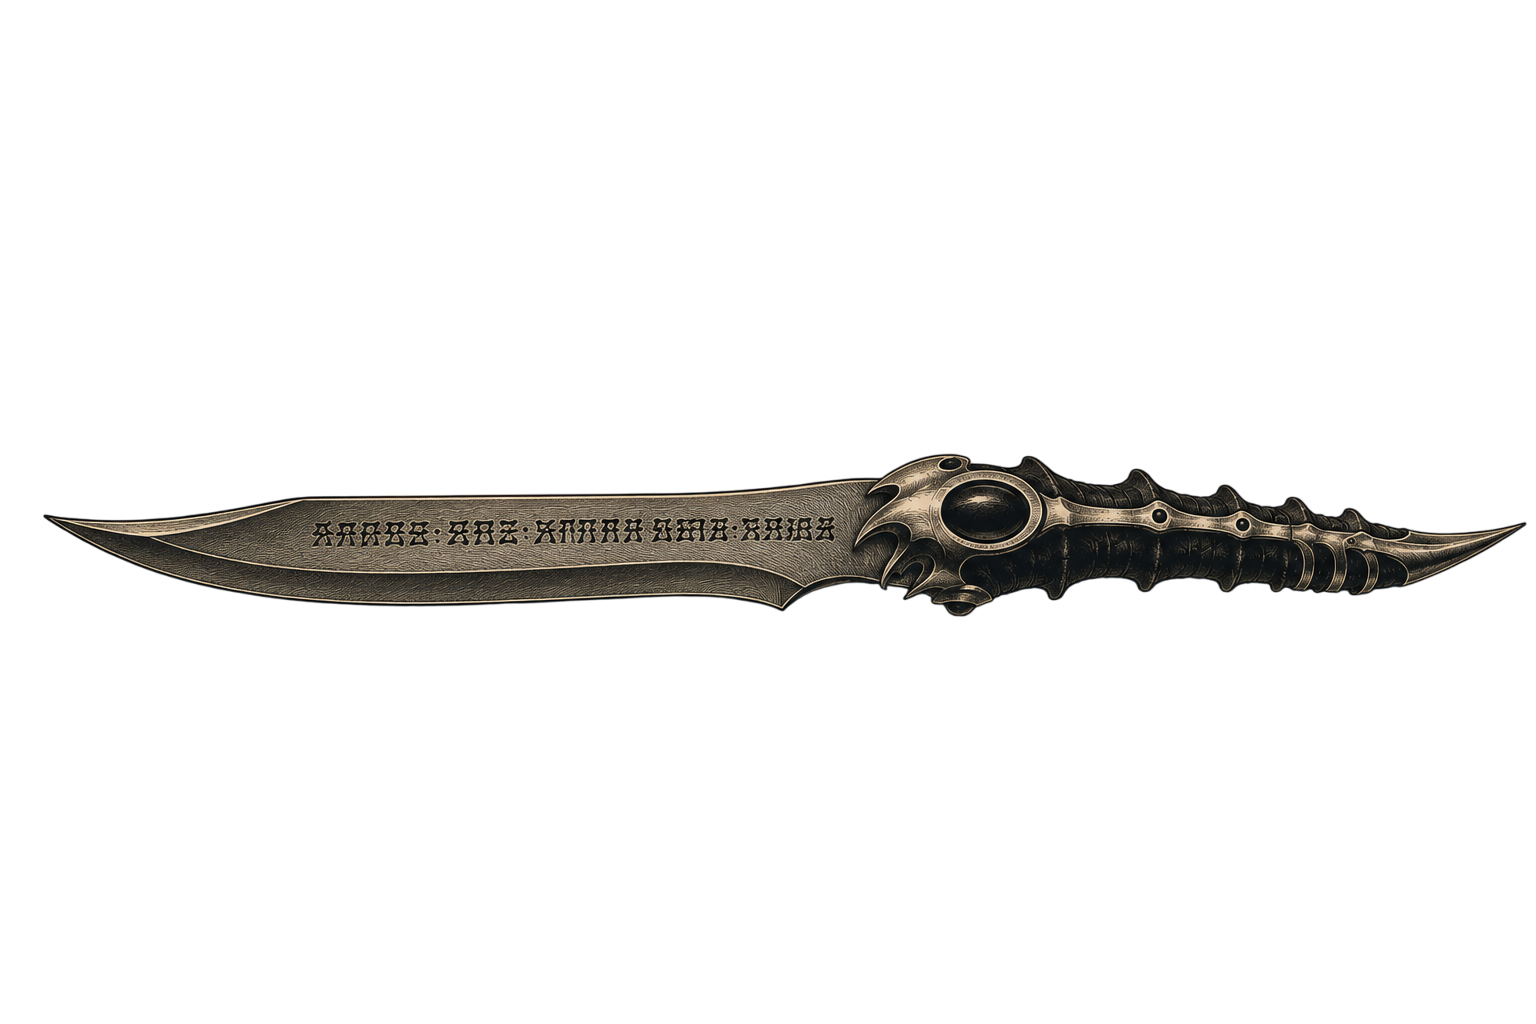
\includegraphics[width=0.50\textwidth]{Photo24.png}

  \vspace{24pt}
  {\large\itshape Thank you for reading.\par}
  \vspace{30pt}
  {\Large\scshape A Dream of Ash and Iron\par}
  \vspace{12pt}
  {\large Written by Navneet Patel\par}
  \vspace{6pt}
  {\normalsize\itshape An ASOIAF\,/\,Game of Thrones Fan Fiction\par}
  \vspace{30pt}
  {\small\itshape This story was written out of love for the world\\
  George R.\,R.\ Martin built and the characters\\
  he gave us to care about.\par}
  \vspace{24pt}
  {\small 2026\par}
\end{center}

\end{document}
